% #5 | Archive/SP_SauLuoi_2024-2025/SP_HKI/1-TN-DS-TLN-THPT-ThuanThanhSo1-BacNinh-HKI-NH24-25.tex | mã gốc 1H4V4-6
\begin{ex}%[Đề thi HK1 lớp 11 THPT Thuận Thành Số 1-24-25]%[Nguyễn Chiến]%[1H4V4-6]
 ($1{,}5$ điểm) Cho hai hình bình hành $ABCD$ và $ABEF$ không cùng nằm trong một mặt phẳng.
\begin{enumerate}
\item Chứng minh rằng $\left(AFD\right) \parallel \left(BEC\right)$.
\item Gọi $M$ là trọng tâm của tam giác $ABE$. Gọi $(P)$ là mặt phẳng đi qua $M$ và song song với mặt phẳng $(AFD)$. Lấy $N$ là giao điểm của $(P)$ và $AC$. Tính $\dfrac{AN}{NC}$.
 \end{enumerate}
\loigiai{
\immini{
\begin{enumerate}
		\item Ta có $AD\parallel BC$, suy ra $AD\parallel (BCE)$.\\
		 Tương tự $AF\parallel BE$, suy ra $AF\parallel (BCE)$.\\
		Do đó $(ADF)\parallel (BCE)$.
		\item Ta có $(P)\parallel(AFD)$ nên $(P)\cap (ABF)=MH$ với $M\in AB$ và $MH\parallel AF$.\\
		Vì $M$ là trọng tâm của tam giác $ABE$ nên $\dfrac{BM}{BO}=\dfrac{2}{3}$ với $O$ là tâm hình bình hành $ABEF$.\\
		Vì $ABEF$ là hình bình hành nên $\dfrac{BO}{BF}=\dfrac{1}{2}$. Suy ra $\dfrac{BM}{BF}=\dfrac{1}{3}$. Do đó $\dfrac{BM}{MF}=\dfrac{1}{2}$.\\
		Khi đó $\dfrac{BH}{AH}=\dfrac{1}{2}$ (vì $AF\parallel MH$).\\
		$(P)\parallel(AFD)$ nên $(P)\cap (ABC)=NH$ với $N\in AC$ và $NH\parallel AD$.\\	
Do đó $\dfrac{AN}{NC}=\dfrac{AH}{BH}=2$.
\end{enumerate}}{
\begin{tikzpicture}[scale=0.6, font=\footnotesize, line join=round, line cap=round, >=stealth]
\coordinate [label= left: $A$](A) at (0,0) ;
\coordinate [label= below: $D$](D) at (-2,-2) ;
\coordinate [label= right: $B$](B) at (7,0) ;
\coordinate [label= below: $C$](C) at ($(B)+(D)-(A)$) ;
\coordinate [label= above: $F$](F) at ($(A)+(-1,4)$) ;
\coordinate [label= above: $E$](E) at ($(B)+(F)-(A)$) ;
%\coordinate [label= below: $O$](O) at ($(A)!0.5!(C)$) ;
\coordinate [label= above: $O$](O) at ($(A)!0.5!(E)$) ;
\coordinate [label= above: $M$](M) at ($(B)!1/3!(F)$) ;
\coordinate [label= above left: $H$](H) at ($(B)!1/3!(A)$) ;
\coordinate [label= below: $N$](N) at ($(C)!1/3!(A)$) ;
\draw (C)--(E)--(F)--(D)--(C)--(B)--(E) ;
\draw[dashed] (D)--(A)--(F)--(B)--(A)--(C) (A)--(E) (M)--(H)--(N);
\foreach \i in {A,B,C,D,E,F,O,M,H,N} \draw[fill=black] (\i) circle(1.1pt)  ;
\end{tikzpicture}
}				
}
\end{ex}

% #10 | Archive/SP_SauLuoi_2024-2025/SP_HKI/1-TN-DS-TLN-THPT-NguyenThiMinhKhai-HCM-HKI-NH24-25.tex | mã gốc 1H4V4-6
\begin{bt}%[1H4V4-6]%[KNTT - Lớp 11 - Ôn tập giữa học kì 1 - Đề Nguyễn Thị Minh Khai]%[Thanh Phát]
	Cho hình chóp $S.ABCD$ có đáy $ABCD$ là hình bình hành tâm $O$. Lấy $M$ trên cạnh $SA$ sao cho $MA=2MS$, $N$ trên cạnh $BC$ sao cho $NB=2NC$ và $G$ là trọng tâm tam giác $BCD$.
	\begin{enumerate}
		\item Tìm giao tuyến của hai mặt phẳng $(SAD)$ và $(MBC)$.
		\item Chứng minh $(MNG)$ song song với $(SCD)$.
		\item Cho biết tam giác $SCD$ vuông tại $S$ có $SC=3$, $SD=4$. Tính tỉ số $\dfrac{MN}{AB}$.
	\end{enumerate}
	\loigiai{
	\begin{enumerate}
	\immini{
		\item Ta có $\heva{&M\in (SAD)\cap (MBC)\\ &AD \parallel BC\\ &AD\subset (SAD),\, BC\subset (MBC).}$\\
		Suy ra $(SAD)\cap (MBC)=d$ với $d$ qua $M$ và song song với $AD$, $BC$.
		\item Vì $G$ là trọng tâm của tam giác $BCD$.\\
		Nên $CG=\dfrac{2}{3}CO=\dfrac{1}{3}CA\Rightarrow CG=\dfrac{1}{2}AG$.\\
		Xét $\triangle SAC$ có $\dfrac{MA}{MS}=\dfrac{GA}{GC}=2$.\\
		Suy ra $MG\parallel SC $ (định lí Thales đảo).\\
		Xét $\triangle ABC$ có $\dfrac{NB}{NC}=\dfrac{GA}{GC}=2$.\\
		Suy ra $NG\parallel AB$ (định lí Thales đảo).\\
		Mà $AB \parallel CD $.
		Do đó $NG\parallel CD$.\\
		Ta có $\heva{&MG\parallel SC \, \text{(cmt)}\\&NG\parallel CD \, \text{(cmt)} \\ &MG,\, NG \subset (MNG)\\ &SC,\, CD\subset (SCD).}$\\
		Suy ra $(MNG)\parallel (SCD)$.}
		{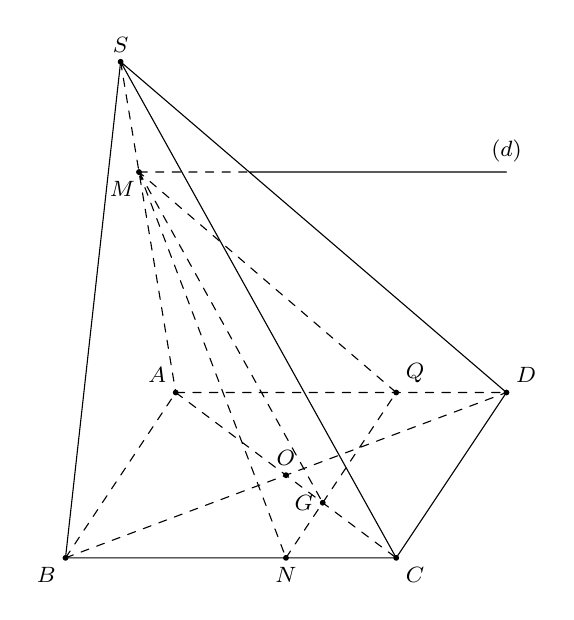
\begin{tikzpicture}[scale=0.7, font=\footnotesize, line join=round, line cap=round, >=stealth]
				\draw[fill=black] (0,0) node[above left]{$A$} coordinate (A) circle(1.2pt);
				\draw[fill=black] (-2,-3) node[below left]{$B$} coordinate (B) circle(1.2pt);
				\draw[fill=black] (4,-3) node[below right]{$C$} coordinate (C) circle(1.2pt);
				\draw[fill=black] (6,0) node[above right]{$D$} coordinate (D) circle(1.2pt);
				\draw[fill=black] (-1,6) node[above]{$S$} coordinate (S) circle(1.2pt);
				\draw[fill=black] (2,-1.5) node[above]{$O$} coordinate (O) circle(1.2pt);
				\draw[fill=black] (2,-3) node[below]{$N$} coordinate (N) circle(1.2pt);
				\draw[fill=black] (4,0) node[above right]{$Q$} coordinate (Q) circle(1.2pt);
				\draw[fill=black] (8/3,-2) node[left]{$G$} coordinate (G) circle(1.2pt);
				\draw[fill=black] (-2/3,4) node[below, xshift=-6pt]{$M$} coordinate (M) circle(1.2pt);
				\draw[fill=black] (4/3,4) coordinate (M');
				\draw[fill=black] (6,4) node[above]{$(d)$} coordinate (d);
				\draw (S)--(B) (S)--(B) (S)--(C) (S)--(D) (B)--(C)--(D) (M')--(d);
				\draw[dashed] (A)--(C) (B)--(D) (S)--(A) (B)--(A)--(D) (N)--(Q)--(M) (M)--(M') (M)--(N) (M)--(G);
			\end{tikzpicture}
		}
		\item Ta có $AB=CD=\sqrt{SC^2 + SD^2}=5$.\\
		Vì $\heva{&(MNG)\parallel (SCD)\\ &(SAD)\cap (SCD)=SD.}$\\
		Nên $(SAD)\cap (MNG)= MQ\parallel SD $ ($Q\in AD$).\\
		Suy ra $\dfrac{MQ}{SD}=\dfrac{AM}{AS}=\dfrac{2}{3} \Rightarrow MQ=\dfrac{2}{3}SD=\dfrac{8}{3}$.\\
		Ta có $\heva{&MG=\dfrac{2}{3}SC=\dfrac{2}{3}\cdot 3 =2 \\ &GQ=\dfrac{2}{3}CD = \dfrac{2}{3}\cdot 5 = \dfrac{10}{3}\\ & MQ=\dfrac{8}{3}.}$\\
		Suy ra $MG^2 + MQ^2 = GQ^2$.\\
		Do đó $\triangle MGQ$ vuông tại $M$.\\
		Khi đó $\cos \left( \widehat{MQN} \right) =\dfrac{MQ}{GQ}=\dfrac{4}{5}$.\\
		Áp dụng định lí cosin cho tam giác $MNQ$ ta có
		\begin{align*}
			MN^2 &= QM^2 + QN^2 - 2\cdot QM \cdot QN \cdot \cos \left(\widehat{MQN} \right)\\
			&= \left(\dfrac{8}{3} \right)^2 + 5^2 - 2\cdot \dfrac{8}{3}\cdot 5\cdot \dfrac{4}{5}\\
			&= \dfrac{97}{5}.
		\end{align*}
		Do đó $MN=\dfrac{\sqrt{97}}{3}$. Suy ra $\dfrac{MN}{AB}=\dfrac{\sqrt{97}}{15}$.
	\end{enumerate}
	}
\end{bt}

% #13 | Archive/SP_SauLuoi_2024-2025/SP_HKI/1-TL-TN-DS-THPT-VoThiSau-GHKI-HCM-NH24-25.tex | mã gốc 1H4H1-4
\begin{ex}%[1H4H1-4]%[Lớp 11-THPT Võ Thị Sáu-GHKI-TP HCM]%[Nguyễn Hữu Đức]
Cho hình chóp $S.ABCD$ có đáy $ABCD$ là hình thang đáy lớn $AB$. Gọi $M$ trung điểm của $SB$. Tìm
\begin{enumerate}
	\item Giao tuyến hai mặt phẳng $(MAD)$ và $(SBC)$.
	\item Giao điểm của đường thẳng $DM$ và $(SAC)$.
\end{enumerate}
\loigiai{
	\begin{center}
		\begin{tikzpicture}[font=\footnotesize, line join=round, line cap=round, >=stealth,scale=1]
			\path
			(0,0) coordinate (A) 
			(7,0) coordinate (B)
			(-2,-2) coordinate (D)
			(1.2,-2) coordinate (C)
			
			(0.5,4) coordinate (S)
		%	($(A)!.5!(C)$) coordinate (O)
			($(B)!.5!(S)$) coordinate (M)
			(intersection of A--C and B--D) coordinate (O)
			(intersection of D--M and S--O) coordinate (I)
			(intersection of D--A and B--C) coordinate (J)
			;
			\draw 
			(S)--(B)--(C)--(D)--cycle
			(S)--(C) (D)--(J) (J)--(C) (M)--(J);
			\draw [dashed] (S)--(A)--(D)--(B)--(A)--(C) (M)--(D) (M)--(A) (S)--(O);
			%\draw (2.75,2)--(0.9,1)node[above]{$d$};
			\foreach \x/\g in
			{A/150,B/10,C/0,D/180,S/90,O/45,M/80,J/-90,I/128}
			\fill (\x) circle (1pt)
			($(\x)+(\g:3mm)$) node{$\x$};
		\end{tikzpicture} 
	\end{center}
	
	\begin{enumerate}
		\item Giao tuyến hai mặt phẳng $(MAD)$ và $(SBC)$.\\
		Trong mặt phẳng $(ABCD)$,
		gọi $J=AD \cap BC$.\\
		Suy ra $MJ=(MAD) \cap(SBC)$.
		\item Giao điểm của đường thẳng $DM$ và $(SAC)$.\\
		Trong mặt phẳng $(SBD)$,
		gọi $I=SO \cap DM$.\\
		Vậy $DM \cap(SAC)=I$.
	\end{enumerate}
}
\end{ex}

% #41 | Archive/SP_SauLuoi_2024-2025/SP_HKI/1-TN-TL-THPT-MacDinhChi-TPHCM-HKI-NH24-25.tex | mã gốc 1H4V4-6
\begin{ex}%[1H4V4-6]%[Dự án đề kiểm tra Toán 11 HKI NH24-25 - Đoàn Minh Tâm]%[THPT Mạc Đĩnh Chi]
Cho hình chóp $S.ABCD$ có đáy $ABCD$ là hình thang ($ AB\parallel CD$), $ AB=2CD$, $ O=AC\cap BD$. Gọi $M$, $N$, $P$ lần lượt là trung điểm của các cạnh $SA$, $AB$, $AD$.
\begin{enumerate}
	\item Tìm giao tuyến của hai mặt phẳng $\left(SBD\right)$ và $\left(SCN\right)$.
	\item Chứng minh $\left(MNP\right)\parallel\left(SBD\right)$.
	\item Gọi $I$ là giao điểm của $SB$ và mặt phẳng $\left(OMP\right)$. Tính tỉ số $\dfrac{IS}{IB}$.
\end{enumerate}
\loigiai{
	\begin{center}
		\begin{tikzpicture}[line join=round,line cap=round,line width=.6pt,font=\footnotesize,scale=1.4]
			\coordinate[label=left:$A$] (A) at (0,0);
			\coordinate[label=below left:$D$] (B) at (.5,-1.4);
			\coordinate[label=below right:$C$] (C) at (3.5,-1.4);
			\coordinate[label=right:$B$] (D) at (6,0);
			\coordinate[label=above left:$S$] (S) at (1.2,3.5);
			\coordinate[label=left:$M$] (M) at ($(S)!1/2!(A)$);
			\coordinate[label=below left:$P$] (N) at ($(A)!1/2!(B)$);
			\coordinate[label=above right:$N$] (P) at ($(A)!1/2!(D)$);
			\coordinate[label=above:$I$] (I) at ($(S)!1/3!(D)$);
			\coordinate[label=below:$O$] (O) at ($(B)!1/3!(D)$);
			\path[name path=bd] (B)--(D); % Đặt tên đoạn thẳng AB là ab
			\path[name path=cn] (C)--(P); % Đặt tên đoạn thẳng CD là cd
			\path[name intersections={of= bd and cn,by=Q}];
			\path (Q) node[above right]{$Q$};
			\draw (A)--(B)--(C)--(D)--(S)--cycle (B)--(S)--(C) (M)--(N);
			\draw[dashed] (A)--(D)--(B) (N)--(P)--(M) (S)--(P)--(C) (I)--(O)--(N)--(M)--(O);
			\fill (A)circle(1.5pt) (B)circle(1.5pt) (C)circle(1.5pt) (D)circle(1.5pt) (S)circle(1.5pt) (M)circle(1.5pt) (N)circle(1.5pt) (P)circle(1.5pt) (Q)circle(1.5pt) (I)circle(1.5pt) (O)circle(1.5pt);
		\end{tikzpicture}
	\end{center}
	\begin{enumerate}
		\item Ta có $S$ là điểm chung thứ nhất của hai mặt phẳng $(S B D)$ và $(S C N)$.\\
		Trong mặt phẳng $(A B C D)$, gọi $Q=C N \cap B D$.\\
		Ta có $Q$ là điểm chung thứ hai của hai mặt phẳng $(S B D)$ và $(S C N)$.\\
		Nên giao tuyến của hai mặt phẳng $(S B D)$ và $(S C N)$ là đường thẳng $S Q$.
		\item Ta có $N P \parallel B D$ (Vì $N P$ là đường trung bình của $\triangle A B D$).\\
		Tương tự $M P \parallel S D$ (Vì $M P$ là đường trung bình của $\triangle S A D$).\\
		Và $M P$, $N P \subset(M N P)$; $B D$, $S D \subset(S B D)$; $N P \cap M P=P$.\\
		Suy ra $(M N P) \parallel(S B D)$.
		\item 	Xét hai mặt phẳng $(O M P)$ và $(S B D)$ có điểm $O$ chung và $M P \parallel S D$.\\
		Nên $(O M P) \cap(S B D)=d$ với $d$ đi qua $O$ và $d \parallel M P \parallel S D$.\\
		$d$ cắt $S B$ tại $I \Rightarrow I=S B \cap(O M P)$.\\
		Ta có $\triangle O A B$ đồng dạng $\triangle O C D \Rightarrow \dfrac{O D}{O B}=\dfrac{C D}{A B}=\dfrac{1}{2}$.\\
		Ta có $I O \parallel S D \Rightarrow \dfrac{I S}{I B}=\dfrac{O D}{O B}=\dfrac{1}{2}$.
	\end{enumerate}
}
\end{ex}

% #50 | Archive/SP_SauLuoi_2024-2025/SP_HKI/1-TL-TN-DS-THPT-Hoang-Viet-Daklak-HKI-NH24-25.tex | mã gốc 1H4V2-4
\begin{bt}%[1H4V2-4]%[Dự án đề kiểm tra Toán 11 HKI NH24-25-Dot5-Thanh Phong]%[TH,THCS & THPT Hoàng Việt - Đăklăk]
Cho hình lăng trụ tam giác $ABC.A'B'C'$. Gọi $M$, $N$, $P$ lần lượt là trung điểm của các cạnh $AB$, $BC$ và $AA'$.
\begin{enumerate}[a)]
	\item Xác định giao điểm $K$ của mặt phẳng $\left(MNP\right)$ và đường thẳng $B'C$.
	\item Tính tỉ số $\dfrac{KB'}{KC}$.
\end{enumerate}
\loigiai{
	\begin{enumerate}[a)]
		\item 
		\immini{Xét hai mặt phẳng $(MNP)$ và $(ACC'A')$ có $\heva{&P\in\left(MNP\right)\cap\left(ACC'A'\right)\\&MN\parallel AC\\&MN\subset\left(MNP\right)\\&AC\subset\left(ACC'A'\right).}$\\ 
		$\Rightarrow\left(MNP\right)\cap\left(ACC'A'\right)=PQ\parallel MN\parallel AC$, $Q\in CC'$.\\
		Trong mặt phẳng $(BCC'B')$ gọi $K=QN\cap CB'$.\\
		Suy ra $K=B'C\cap (MNP)$.}
		{\begin{tikzpicture}[scale=0.9,font=\footnotesize,line join = round, line cap = round, >= stealth]
			\coordinate (A) at (0,0);
			\def\x{4}
			\def\y{2}
			\def\z{3}
			\def\g{-60}% goc  đáy
			\def\n{85} %goc nghiêng
			\coordinate (B) at ($(A)+(\x,0)$);
			\coordinate (C) at ($(A)+(\g:\y)$);
			\coordinate (A') at ($(A)+(\n:\z)$);
			\coordinate (B') at ($(B)+(\n:\z)$);
			\coordinate (C') at ($(C)+(\n:\z)$);
			\coordinate (M) at ($(A)!.5!(B)$);
			\coordinate (N) at ($(C)!.5!(B)$);
			\coordinate (P) at ($(A)!.5!(A')$);
			\coordinate (Q) at ($(C)!.5!(C')$);
			\coordinate (E) at ($(C)!.5!(B')$);
			\coordinate (K) at ($(N)!.5!(Q)$);
			\draw (A)--(C)--(C')--(A')--cycle;
			\draw (A')--(B')--(C') (B')--(B)--(C)--(C');
			\draw[dashed] (A)--(B);
			\draw (P)--(Q)--(N) (B)--(C') (C)--(B');
			\draw[dashed] (P)--(M)--(N);
			\foreach \p/\g in {A/-120,B/-90,C/-45,A'/180,B'/90,C'/70,M/90,N/-90,P/160,Q/-130,E/10,K/-90} \draw[blue,fill=white] (\p) circle(.5pt) node [shift={(\g:.3)}] {$\p$};
			\end{tikzpicture}}
		\item Gọi $E$ là tâm hình bình hành $BCC'B'$.\\
		Do $P$ là trung điểm $AA'$ nên $Q$ là trung điểm $CC'$.\\
		Suy ra $QN$ là đường trung bình của tam giác $CBC'$.\\
		Do đó $K$ là trung điểm của $CE$.\\
		Vậy $\dfrac{KB'}{KC}=3$.
	\end{enumerate}
 }
\end{bt}

% #56 | Archive/SP_SauLuoi_2024-2025/SP_HKI/1-TN-DS-TLN-ChuyenLeQuyDon-NinhThuan-HKI-NH24-25.tex | mã gốc 1H4V4-7
\begin{ex}%[1H4V4-7]%[1H4V4-4]%[1-TN-DS-TLN-ChuyenLeQuyDon-NinhThuan-HKI-NH24-25]%[Thầy Hải Toán]
	Nhà bạn Lan có một đèn trang trí khung hình chóp tam giác $S.ABC$. Vị trí bóng đèn tiếp xúc với mặt đáy $(ABC)$ tại trọng tâm $G$ của tam giác $ABC$. Mẹ Lan nhờ Lan xác định vị trí điểm $M$ trên cạnh $SA$ của đèn. Biết rằng $M$ là giao điểm của $SA$ với mặt phẳng $(\alpha)$, và mặt phẳng
	$(\alpha)$ đi qua $G$ và song song với mặt phẳng $(SBC)$. Em hãy giúp Lan tính tỉ số $\dfrac{SM}{AM}$.
	\begin{center}
		
\begin{tikzpicture}[line cap=round,line join=round]
		\path[draw=gray, fill] (0, 6) -- (-0.08, 6) -- (-0.08, 5.22) -- (-0.15, 5.18) --
			(-0.15, 4.96) .. controls +(0:0) and +(90:0.04) ..
			(-0.23, 4.89) .. controls +(-90:0.04) and +(0:0) ..
			(-0.19, 4.81) -- (-0.19, 4.43) -- (-0.56, 3.45) .. controls +(0:0) and +(89:0.36) ..
			(-0.56, 2.38) -- (0.52, 2.38) .. controls +(91:0.36) and +(0:0) ..
			(0.52, 3.45) -- (0.15, 4.43) -- (0.15, 4.81) .. controls +(0:0) and +(-90:0.04) ..
			(0.19, 4.89) .. controls +(90:0.04) and +(0:0) ..
			(0.11, 4.96) -- (0.11, 5.18) -- (0.04, 5.22) -- (0.04, 6) --
			(-0.04, 6);

		\def\bongden{(-0, -0.21) .. controls +(178:0.68) and +(-88:0.82) ..
			(-1.24, 1.1) .. controls +(92:0.32) and +(-160:0.5) ..
			(-0.56, 2.06) .. controls +(53:0.07) and +(-81:0.07) ..
			(-0.48, 2.23) .. controls +(96:0.07) and +(-90:0.04) ..
			(-0.56, 2.38) .. controls +(13:0.36) and +(168:0.36) ..
			(0.52, 2.38) .. controls +(-90:0.04) and +(84:0.07) ..
			(0.44, 2.23) .. controls +(-96:0.07) and +(127:0.07) ..
			(0.52, 2.06) .. controls +(-20:0.5) and +(89:0.32) ..
			(1.2, 1.1) .. controls +(-92:0.82) and +(2:0.68) ..
			(-0.04, -0.21);}

		\path[inner color=orange, outer color=yellow] \bongden

		\path[top color=black, bottom color=gray, even odd rule]
			(-3.62, 0) -- (-0.38, -1.06) -- (3.5, 0) --cycle
			(-1.39, -0.24) -- (-0.59, -0.51) -- (-0.58, -0.24) --cycle
			(-0.06, -0.24) -- (-0.05, -0.55) -- (1.09, -0.25) --cycle;

		\path[top color=black, bottom color=gray!35!black, even odd rule]
			(-0.3, 4.67) -- (-3.62, 0) -- (3.5, 0) -- (0.26, 4.67) --cycle
			(0.05, 4.27) -- (-0.1, 4.27) -- (-2.84, 0.41) -- (2.73, 0.41) --cycle;
	\end{tikzpicture}
		\\
		\begin{tikzpicture}[line join = round, line cap = round,>=stealth,font=\footnotesize,scale=1,declare function={ac=5;ab=2.2; gocB=-60;ha=3.5;}]
			\path 
			(0,0) coordinate (A)
			(ac,0) coordinate (C)
			(gocB:ab) coordinate (B)
			($(B)!0.5!(C)$) coordinate (BC)
			($(A)!0.5!(B)$) coordinate (AB)
			(intersection of C--AB and A--BC) coordinate (G)
			($(G)+(0,ha)$) coordinate (S);
			\draw (S)--(A)--(B)--(C)--cycle (S)--(B);
			\draw[dashed] (A)--(C);
			\foreach \x/\gm in {S/90,A/180,B/-90,C/0,G/-90} \fill (\x) circle (1pt) ($(\x)+(\gm:3.5mm)$)node{$\x$};
		\end{tikzpicture}	
	\end{center}
	\loigiai{
		\begin{center}
			\begin{tikzpicture}[line join = round, line cap = round,>=stealth,font=\footnotesize,scale=1,declare function={ac=5;ab=2.2; gocB=-60;ha=3.5;}]
				\path 
				(0,0) coordinate (A)
				(ac,0) coordinate (C)
				(gocB:ab) coordinate (B)
				($(B)!0.5!(C)$) coordinate (BC)
				($(A)!0.5!(B)$) coordinate (AB)
				(intersection of C--AB and A--BC) coordinate (G)
				($(G)+(0,ha)$) coordinate (S)
				($(A)!2/3!(B)$) coordinate (N)
				($(A)!2/3!(C)$) coordinate (P)
				($(A)!2/3!(S)$) coordinate (M)
				;
				\draw (S)--(A)--(B)--(C)--cycle (S)--(B) (M)--(N);
				\draw[dashed] (A)--(C) (M)--(P)--(N);
				\foreach \x/\gm in {S/90,A/180,B/-90,C/0,G/-90,N/-150,M/150,P/70} \fill (\x) circle (1pt) ($(\x)+(\gm:3.5mm)$)node{$\x$};
			\end{tikzpicture}		
		\end{center}
		Trong mặt phẳng $(ABC)$: Qua $G$ kẻ đường thẳng song song $BC$ cắt $AB$ và $AC$ lần lượt tại $N$ và $P$.\\
		Trong mặt phẳng $(SAC)$: Qua $P$ kẻ đường thẳng song song $SC$ cắt $SA$ tại $M$.\\
		Ta có $\heva{& NP\parallel BC \\ & PN\parallel SC \\ & SC\subset (SBC) \\ & BC\subset (SBC) \\ & MP\cap NP=\{P\}}\Rightarrow \left(MNP\right)\parallel\left(SBC\right)$.\\
		$M$ là giao điểm của $\left(\alpha\right)$ với $SA$ suy ra $SA\cap(MNP)=\{M\}$.\\
		Vì $NP\parallel BC$ nên theo định lý talet ta có $\dfrac{AG}{AD}=\dfrac{AN}{AB}=\dfrac{AP}{AC}=\dfrac{2}{3}$.\\
		$MP\parallel SC$ nên theo định lý talet ta có $\dfrac{SM}{AM}=\dfrac{CP}{AP}=\dfrac{1}{2}$.
	}
\end{ex}

% #59 | Archive/SP_SauLuoi_2024-2025/SP_HKI/1-TN-DS-TLN-ChuyenLeQuyDon-NinhThuan-HKI-NH24-25.tex | mã gốc 1H4V4-6
\begin{ex}%[1H4V4-6]%[1-TN-DS-TLN-ChuyenLeQuyDon-NinhThuan-HKI-NH24-25]%[Thầy Hải Toán]
	Cho hình chóp $SABCD$ có đáy $ABCD$ là hình vuông cạnh bằng $6$ và tam giác $SAB$ đều. Điểm $M$ thuộc cạnh $BC$ sao cho $BM=\dfrac{1}{3} BC$. Gọi ($\alpha$) là mặt phẳng đi qua $M$ và song song với $SA$, $CD$. Mặt phẳng $\left(\alpha\right)$ cắt $SC$, $SD$, $AD$ lần lượt tại $N$, $P$, $Q$. Tính diện tích tứ giác $MNPQ$ (Kết quả làm tròn đến hàng phần chục).
	\loigiai{
		\begin{center}
			\begin{tikzpicture}[line join = round, line cap = round,>=stealth,font=\footnotesize,scale=1,declare function={ab=3.2;ad=5;cao=5;gocB=-145;}]
				\path (0,0) coordinate (A)
				(gocB:ab) coordinate (B)
				(ad,0) coordinate (D)
				($(D)-(A)+(B)$) coordinate (C)
				($(A)!0.5!(B)$) coordinate (H)
				($(H)+(100:cao)$) coordinate (S) 
				($(B)!1/3!(C)$) coordinate (M)
				($(A)!1/3!(D)$) coordinate (Q)
				($(S)!1/3!(D)$) coordinate (P)
				($(S)!1/3!(C)$) coordinate (N)
				($(M)!0.3!(Q)$) coordinate (K)
				($(Q)!0.3!(M)$) coordinate (I)
				;
				\draw (S)--(B)--(C)--(D)--(S)--(C) (P)--(N)--(M)
				;
				\draw[dashed] (S)--(A)--(D) (A)--(B) (M)--(Q)--(P) (N)--(K) (P)--(I);
				\foreach \x/\gm in {A/-80,B/-90,C/-90,D/0,S/90,M/-90,Q/70,P/90,N/90,K/-90,I/-90} \fill (\x) circle (1pt) ($(\x)+(\gm:3.5mm)$)node{$\x$};
				\foreach \x/\y/\z in {N/K/M,P/I/Q} \draw pic[draw,angle radius=2.5mm]{right angle=\x--\y--\z};
			\end{tikzpicture}
		\end{center}
		Trong mặt phẳng $(ABCD)$ kẻ $MQ\parallel CD$ cắt $AD$ tại $Q$.\\
		Trong mặt phẳng $(SAD)$ kẻ $QP\parallel SA$ cắt $SD$ tại $P$.\\
		Trong mặt phẳng $(SCD)$ kẻ $PN\parallel CD$ cắt $SC$ tại $N$.\\
		Vậy mặt phẳng $\left(\alpha\right)$ là mặt phẳng $(MQPN)$.\\
		Tam giác $SAB$ đều suy ra $SA=SB=AB=6$.\\
		\begin{itemize}
			\item [\color{teal}\faCheckCircleO] $MQ\parallel CD\Rightarrow\dfrac{CM}{CB}=\dfrac{DQ}{DA}=\dfrac{2}{3}$.
			\item [\color{teal}\faCheckCircleO] $PQ\parallel SA\Rightarrow \dfrac{DP}{DS}=\dfrac{DQ}{DA}=\dfrac{PQ}{SA}=\dfrac{2}{3}\Rightarrow PQ=\dfrac{2}{3}SA=4$.
			\item [\color{teal}\faCheckCircleO] $NP\parallel CD\Rightarrow\dfrac{SN}{SC}=\dfrac{SP}{SD}=\dfrac{NP}{CD}=\dfrac{1}{3}\Rightarrow NP=\dfrac{1}{3}CD=2$.
			\item [\color{teal}\faCheckCircleO] $MQ\parallel CD\Rightarrow\dfrac{CM}{CB}=\dfrac{CN}{CS}=\dfrac{MN}{SB}=\dfrac{2}{3}\Rightarrow MN=4$.
		\end{itemize}
		Trong mặt phẳng $(SBC)$ ta có $\dfrac{CN}{CS}=\dfrac{CM}{CB}=\dfrac{MN}{SB}=\dfrac{2}{3}\Rightarrow NM\parallel SB$.\\
		Vậy $NP\parallel MQ\parallel CD\Rightarrow $ tứ giác $MQPN$ là hình thang.\\
		$\heva{& PQ\parallel SA \\ & MQ\parallel AB}\Rightarrow\widehat{\left(PQ,QM\right)}=\widehat{\left(SA,AB\right)}=\widehat{SAB}$.\\
		$\heva{& MN\parallel SB \\ & MQ\parallel AB}\Rightarrow\widehat{\left(MN,MQ\right)}=\widehat{\left(SB,AB\right)}=\widehat{SBA}$.\\
		Tam giác $SAB$ đều nên suy ra $\widehat{SAB}=\widehat{SBA}=60^\circ\Rightarrow$ tứ giác $MQPN$ là hình thang cân.\\
		Gọi $K$ và $I$ lần lượt là hình chiếu của $N$ và $P$ lên $MQ$. \\
		Ta có $MK=IQ=\dfrac{MQ-IK}{2}=\dfrac{6-2}{2}=2$.\\
		Trong tam giác vuông $PIQ$: $PI=\sqrt{PQ^2-IQ^2}=\sqrt{4^2-2^2}=2\sqrt{3}$.\\
		Diện tích hình thang $MQPN$ là $S_{MQPN}=\dfrac{\left(MQ+NP\right)\cdot PI}{2}=\dfrac{\left(6+2\right)\cdot 2\sqrt{3}}{2}=8\sqrt{3}\approx 13{,}86$ (đơn vị diện tích).
	}
\end{ex}

% #90 | Archive/SP_SauLuoi_2024-2025/SP_HKI/1-TN-DS-TLN-THPT-ChuyenLeHongPhong-TpHCM-HKI-NH24-25.tex | mã gốc 1H4V1-4
\begin{bt}%[1H4V1-4][Dự án đề kiểm tra môn Toán khối 11 HKI NH24-25 - Đợt 5 - Hieu Hieu Minh Minh]%[THPT Chuyên Lê Hồng Phong - Tp HCM]
	Cho hình chóp $S.ABCD$ có đáy là hình thang $ABCD$ với $AD \parallel BC$ và $AD = 2BC$. Gọi $M$ là điểm trên cạnh $SD$ thỏa mãn $SM = \dfrac{1}{3}SD$. Mặt phẳng $(ABM)$ cắt cạnh bên $SC$ tại điểm $N$. Tính tỉ số $\dfrac{SN}{SC}$.
	\loigiai{
		\begin{center}
			\begin{tikzpicture}
				\def\a{4}
				\path (0:0) coordinate (A)
				++(0:1.7*\a) coordinate (D)
				($(A)+(-70:\a/2)$) coordinate (B)
				($(B)+(D)-(A)$) coordinate (Ct)
				($(B)!.5!(Ct)$) coordinate (C)
				($(A)+(75:1.3*\a)$) coordinate (S)
				($(S)!1/3!(D)$) coordinate (M)
				(intersection of A--C and B--D) coordinate (O)
				(intersection of S--O and B--M) coordinate (I)
				(intersection of A--I and S--C) coordinate (N)
				($(O)+(N)-(A)$) coordinate (Ht)
				(intersection of O--Ht and S--C) coordinate (J)
				;
				\draw[dashed] (D)--(A)--(C) (D)--(B)--(M)--(A)--(N) (S)--(O)--(J);
				\draw (A)--(B)--(C)--(D)--(S)--(B)--(N)--(M) (C)--(S)--(A);
				\foreach \x/\g in {A/180,B/-135,C/-45,D/0,S/90,M/10,O/-90,I/130,N/10,J/20}
				\fill (\x) circle (1pt)
				($(\g:3mm)+(\x)$) node {$\x$}; 
			\end{tikzpicture}
		\end{center}
	Gọi $O$ là giao điểm của $AC$ và $BD$.\\
	Gọi $I$ là giao điểm của $SO$ và $BM$;\\
	Gọi $N$ là giao điểm của $AI$ và $SC$.\\
	Suy ra $I=(ABM) \cap SC$.\\
	Do $ABCD$ là hình thang với $AD \parallel BC$ và $AD=2BC$.	
	\[
	\dfrac{OC}{OA}=\dfrac{OB}{OD}=\dfrac{BC}{AD}=\dfrac{1}{2} \Rightarrow \dfrac{OA}{AC}=\dfrac{OD}{BD}=\dfrac{2}{3}.
	\]
	Ta có $OM \parallel SB$ và $\dfrac{OM}{SB}=\dfrac{2}{3} \Rightarrow \dfrac{OI}{SI}=\dfrac{OM}{SB}=\dfrac{2}{3}$.\\
	Kẻ $OJ \parallel AN,\, (J \in AN)$.\\
	Xét tam giác $ANC$ có:\\
	\begin{enumerate}[$\bullet$]
		\item Vì $OJ \parallel AN$ nên $\dfrac{OA}{AC}=\dfrac{2}{3} \Rightarrow \dfrac{NJ}{NC}=\dfrac{2}{3} \Rightarrow \overrightarrow{NC}=\dfrac{3}{2} \overrightarrow{NJ}.$
		\item Vì $IN \parallel OJ \text { nên } \dfrac{SI}{IO}=\dfrac{3}{2} \Rightarrow \dfrac{SN}{NJ}=\dfrac{3}{2} \Rightarrow \overrightarrow{SN}=\dfrac{3}{2} \overrightarrow{NJ}$.
	\end{enumerate}
	Do đó $\overrightarrow{SN}=\overrightarrow{NC} \Rightarrow \overrightarrow{SN}=\dfrac{1}{2} \overrightarrow{SC} \Rightarrow \dfrac{SN}{SC}=\dfrac{1}{2}$.
	}
\end{bt}

% #123 | Archive/SP_SauLuoi_2024-2025/SP_GHKI/1-TN-DS-TL-THPT-TranPhu-TpHCM-GHKI-NH24-25.tex | mã gốc 1H4V3-6
\begin{ex}%[1H4V3-6]%[THPT Trần Phú - TP HCM - 2024 - đợt 3]%[TheHung Nguyen]
	Cho hình chóp $S. ABCD$ có đáy $ABCD$ là hình thang, $AD$ song song với $BC$ và $AD=3BC$. Gọi $O$ là giao điểm của $AC$ và $BD$, $E$ và $F$ lần lượt thuộc cạnh $SA$ và $SD$ sao cho $SE=2EA$ và $FD=3FS$.
	\begin{enumerate}
		\item Tìm giao tuyến của hai mặt phẳng $(SAD)$ và $(SBC)$.
		\item  Chứng minh đường thẳng $OF$ song song với mặt phẳng $(SBC)$.
		\item  Tìm giao tuyến $d$ của hai mặt phẳng $(SAB)$ và $(AFC)$. Gọi $I$ là giao điểm của $ED$ và $AF$, chứng minh ba đường thẳng $EB$, $IO$ và $d$ đồng quy tại $K$.	
	\end{enumerate}
	\loigiai{\begin{center}
			\begin{tikzpicture}[scale=1, font=\footnotesize, line join=round, line cap=round, >=stealth]
				\def\a{6}
				\def\b{2}
				\def\h{6}
				\def\g{130}
				\path
				(0,0) coordinate (A)
				(0:\a) coordinate (D)
				--++(-\g:4) coordinate (C)
				--++(-180:\b)coordinate (B)
				;
				\path(intersection of A--C and B--D)coordinate (O);	 
				\coordinate (S) at ($(O)+(0,\h)$);	
				\coordinate (E) at ($(S)!2/3!(A)$); 
				\coordinate (F) at ($(S)!1/4!(D)$); 
				\path(intersection of E--D and A--F)coordinate (I)	
				(intersection of E--B and O--I)coordinate (K)	
				;	
				\draw (S)--++(0:5)coordinate (x) node[above]{$x$};	
				\draw (C)--(S)--(B)--(C)--(D)--(S)--(A)--(B) (C)--(F) (B)--(K)--(A);
				\draw[dashed] (A)--(B) (A)--(C) (B)--(D)--(A) (E)--(D) (A)--(F)--(O)--(K);
				\foreach \x/\g in {A/120,B/-90,C/-90,D/0,S/90,E/130,O/-90,F/45,I/90,K/90}  \fill (\x) circle (1pt)+(\g:.25)node {$\x$};
			\end{tikzpicture}
		\end{center}
		\begin{enumerate}
			\item Ta có $\heva{&S\in (SAD), \, S\in (SBC)\\& AD\parallel BC\\&AD \subset (SAD); BC\subset (SBC)}\Rightarrow (SAD)\cap (SCB)=Sx, (\text{với}\, Sx\parallel AD\parallel BC).$
			\item Xét $(ABCD)$, có $BC\parallel AD$ nên $\dfrac{OD}{OB}=\dfrac{AD}{BC}=3$ mà $\dfrac{FD}{FS}=3$ nên $\dfrac{OD}{OB}=\dfrac{FD}{FS}$.\\
			Xét $\triangle SBD$, có $\dfrac{OD}{OB}=\dfrac{FD}{FS}$ nên $OF\parallel SB$ mà $SB \subset (SBC)$ do đó $OF\parallel (SBC)$. 
			\item Ta có $\heva{&A\in (SAB), A\in (AFC)\\
				&SB\parallel FO, OF\subset (AFC)&SB \subset (SAB)}\Rightarrow (SAB)\cap (AFC)=d,(\text{với}\, A\in d  \,\text{và}\, d\parallel SB\parallel FO)$.\\
			Trong $(AFC)$ gọi $K=d\cap IO$.\\
			Ta có $\heva{&K\in (ABK), K\in (KBD)\\& E\in (ABK),\, E\in (KBD)\\&B\in (ABK),\, B\in (KBD)}\Rightarrow K, E, B$ thẳng hàng, suy ra $EB$, $IO$ và $d$ đồng quy tại $K$.	
		\end{enumerate}	
	}
\end{ex}

% #719 | Archive/2024/TOAN_11_XE/TOAN_11_XE/data4/11C4/BTTN5.tex | mã gốc 1T4B5-3
\begin{bt}%[TeX hóa SGK CTST]%[Trúc Danh]%[1T4B5-3]
	\hfill
	\begin{enumerate}
		\item Tìm hình chiếu song song của đoạn thẳng $AC$, tia $AB$ và đường thẳng $AD$ trong Hình b).
		\item Quan sát Hình a) và so sánh hai ti số $\dfrac{AB}{CD},\dfrac{A'B'}{C'D'}$.
		\item Quan sát Hình b) và so sánh hai tỉ số $\dfrac{DA}{DB},\dfrac{D'A'}{D'B'}$.
	\end{enumerate}
	\begin{center}
		\begin{tikzpicture}[scale=1,font=\footnotesize, line join=round, line cap=round, >=stealth]
			\path 
			(0,0) coordinate (M)
			(4,0) coordinate (N)
			(1,1.5) coordinate (Q)
			($(N)+(Q)-(M)$) coordinate (P)
			(0,.7) coordinate (m)
			(0.8,3) coordinate (m')
			(1.2,.5) coordinate (C')
			(2.8,.5) coordinate (D')
			($(C')+(0.8,2)$) coordinate (C)
			($(D')+(0.6,1.5)$) coordinate (D)
			(2.5,1) coordinate (A')
			(3.5,1) coordinate (B')
			($(A')+(0.8,2)$) coordinate (A)
			($(B')+(0.6,1.5)$) coordinate (B)
			;
			
			\draw (M)--(N)--(P)--(Q)--(M) (C)--(C') (D)--(D') (A)--(A') (B)--(B');
			\draw[red] (m)--(m');
			\draw[cyan,shorten <=-.5cm,shorten >=-.5cm] (C')--(D');
			\draw[cyan,shorten <=-.5cm,shorten >=-.5cm] (C)--(D);
			\draw[blue,shorten <=-.5cm,shorten >=-.5cm] (A')--(B');
			\draw[blue,shorten <=-.5cm,shorten >=-.5cm] (A)--(B);
			\path (m)--(m') node[left,pos=.8]{$l$};
			\pic[draw,"$P$", angle eccentricity=0.6,angle radius=0.5cm]{angle=N--M--Q};
			\foreach \x/\g in {C'/-90,D'/-90,A'/-90,B'/-90,C/40,D/40,A/40,B/40} \fill[black] (\x) circle (1pt)+(\g:.3) node {$\x$};
			\path (2,-.5) node{a)};
		\end{tikzpicture}\hspace{2cm}
		\begin{tikzpicture}[scale=1,font=\footnotesize, line join=round, line cap=round, >=stealth]
			\path 
			(0,0) coordinate (M)
			(4,0) coordinate (N)
			(1,1.5) coordinate (Q)
			($(N)+(Q)-(M)$) coordinate (P)
			(0,.7) coordinate (m)
			(0.8,3) coordinate (m')
			(1,1) coordinate (n)
			(4,.6) coordinate (n')
			(1.5,3) coordinate (p)
			(4,2.5) coordinate (p')
			($(n)!.1!(n')$) coordinate (A')
			($(n)!.4!(n')$) coordinate (B')
			($(n)!.65!(n')$) coordinate (C')
			($(n)!.8!(n')$) coordinate (D')
			($(A')+(0.6,1.8)$) coordinate (A)
			($(D')+(0.3,1.2)$) coordinate (D)
			($(A)!.45!(D)$) coordinate (B)
			($(A)!.8!(D)$) coordinate (C)
			
			;
			\draw (M)--(N)--(P)--(Q)--(M) (C)--(C') (D)--(D') (A)--(A') (B)--(B');
			\draw[red] (m)--(m');
			\draw[violet] (n)--(n');
			\draw[violet,shorten <=-.5cm,shorten >=-.5cm] (A)--(D);
			\path (m)--(m') node[left,pos=.8]{$l$};
			\pic[draw,"$P$", angle eccentricity=0.6,angle radius=0.5cm]{angle=N--M--Q};
			\foreach \x/\g in {C'/-90,D'/-90,A'/-90,B'/-90,C/40,D/40,A/40,B/40} \fill[black] (\x) circle (1pt)+(\g:.3) node {$\x$};
			\path (2,-.5) node{b)};
		\end{tikzpicture}
	\end{center}
	\loigiai{
		\begin{enumerate}
			\item Trong Hình b), hình chiếu song song của đoạn thẳng $AC$, tia $AB$ và đường thẳng $AD$ lần lượt là đoạn thẳng $A'C'$, tia $A'B'$ và đường thẳng $A'D'$.
			\item Do phép chiếu song song không làm thay đồi tỉ số độ dài của các đoạn thẳng nằm trên hai đường thẳng song song nên trong Hình a), ta có $\dfrac{AB}{CD}=\dfrac{A'B'}{C'D'}$.
			\item Do phép chiếu song song không làm thay đổi tỉ số độ dài của các đoạn thẳng cùng thuộc một đường thẳng nên trong Hình b), ta có $\dfrac{DA}{DB}=\dfrac{D'A'}{D'B'}$.
		\end{enumerate}
		
	}
\end{bt}

% #721 | Archive/2024/TOAN_11_XE/TOAN_11_XE/data4/11C4/BTTN5.tex | mã gốc 1T4B5-1
\begin{bt}%[TeX hóa SGK CTST]%[Trúc Danh]%[1T4B5-1]
	Vẽ hình biểu diễn và nêu nhận xét về hình biểu diễn của các mặt của các hình sau
	\begin{multicols}{3}
		\begin{enumerate}
			\item Hình hộp.
			\item Lăng trụ có đáy là lục giác đều.
			\item Tứ diện.
		\end{enumerate}
	\end{multicols}
	\loigiai{
		\begin{center}
			\begin{tikzpicture}[scale=1,font=\footnotesize, line join=round, line cap=round, >=stealth]
				\begin{scope}
					\draw (0,0)--(2,0)--(3,1);
					\draw (0.5,2)--(2.5,2)--(3.5,3)--(1.5,3)--(0.5,2);
					\draw (0,0)--(0.5,2) (2,0)--(2.5,2) (3,1)--(3.5,3);
					\draw[dashed] (1,1)--(1.5,3) (3,1)--(1,1)--(0,0);
					\path (1,-.5) node{a)};
				\end{scope}
				\begin{scope}[shift={(5,1)},rotate=-60]
					\draw 
					(0:1) coordinate (A)--(60:1) coordinate (B)--(120:1) coordinate (C)--(180:1) coordinate (D)--(240:1) coordinate (E)--(300:1) coordinate (F)--(360:1) coordinate (G);
					\draw
					(A)--($(A)+(0.5,3)$) coordinate (A') (B)--($(B)+(0.5,3)$) coordinate (B') (C)--($(C)+(0.5,3)$) coordinate (C')
					(D)--($(D)+(0.5,3)$) coordinate (D'); \draw[dashed]
					(E)--($(E)+(0.5,3)$) coordinate (E')
					(F)--($(F)+(0.5,3)$) coordinate (F')
					(D')--(E')--(F')--(A')
					;
					\draw (A')--(B')--(C')--(D');
					\path (2,.5) node{b)};
				\end{scope}
				\begin{scope}[shift={(10,1)}]
					\draw (0,0)--(1,-1)--(3,0) (0,0)--(1.5,2) (1,-1)--(1.5,2) (3,0)--(1.5,2);
					\draw[dashed] (0,0)--(3,0);
					\path (1,-1.5) node{c)};
				\end{scope}
			\end{tikzpicture}
		\end{center}
		\begin{enumerate}
			\item Hình biểu diễn của các mặt là các hình bình hành.
			\item Hình biểu diễn của mặt đáy là lục giác có các cặp cạnh đối song song và bằng nhau, đồng thời song song với đường chéo nối hai đỉnh còn lại. Hình biểu diễn của mặt bên là hình bình hành.
			\item Hình biểu diễn của bốn mặt là bốn tam giác.
			\item Hình biểu diễn của mặt đáy là elip, hình biểu diễn của các đường sinh là các đoạn thẳng song song và bằng nhau.
		\end{enumerate}
		
	}
\end{bt}

% #722 | Archive/2024/TOAN_11_XE/TOAN_11_XE/data4/11C4/BTTN5.tex | mã gốc 1T4B5-1
\begin{bt}%[TeX hóa SGK CTST]%[Trúc Danh]%[1T4B5-1]
	Trong các mệnh đề sau, mệnh đề nào đúng?
	\begin{enumerate}
		\item Một đường thẳng có thể song song với hình chiếu của nó.
		\item Một đường thẳng có thể trùng với hình chiếu của nó.
		\item Hình chiếu song song của hai đường thẳng chéo nhau có thể song song với nhau.
		\item Hình chiếu song song của hai đường thẳng chéo nhau có thể trùng nhau.
	\end{enumerate}
	\loigiai{
		\begin{enumerate}
			\item Đúng.
			\item Đúng.
			\item Đúng.
			\item Sai, vì hình chiếu song song của hai đường thẳng chéo nhau cắt nhau hoặc song song.
		\end{enumerate}
		
	}
\end{bt}

% #723 | Archive/2024/TOAN_11_XE/TOAN_11_XE/data4/11C4/BTTN5.tex | mã gốc 1T4B5-2
\begin{bt}%[TeX hóa SGK CTST]%[Trúc Danh]%[1T4B5-2]
	Vẽ hình biểu diễn của một lục giác đều.
	\loigiai{
		
		Xét hình lục giác đều $ABCDEF$, ta nhận thấy
		\begin{itemize}
			\item Tứ giác $OABC$ là hình thoi.
			\item Các điểm $D, E, F$ lần lượt là các điểm đối xứng của các điểm $A, B, C$, qua tâm $O$.
		\end{itemize}
		Từ đó suy ra cách vẽ hình biễu diễn của lục giác đều $ABCDEF$ như sau 
		\begin{itemize}	
			\item Vẽ hình bình hành $O'A'B'C'$ biễu diễn cho hình thoi $OABC$.
			\item Lấy các điểm $D', E', F'$ lần lượt đối xứng với các điểm $A', B', C'$ qua $O$, ta được hình biễu diễn $A'B'C'D'E'F'$ của hình lục giác đều $ABCDEF$.
		\end{itemize}
		\begin{center}
			\begin{tikzpicture}[scale=1,font=\footnotesize, line join=round, line cap=round, >=stealth]
				\begin{scope}
					\path (0,0) coordinate (O);
					\foreach \x/\i in {0/A,60/B,120/C,180/D,240/E,300/F}
					{
						\coordinate (\i) at (\x:1);
					}
					\draw (O) circle (1);
					\draw 
					(A)--(B)--(C)--(D)--(E)--(F)--(A)
					(A)--(D) (B)--(E) (C)--(F)
					;
					\foreach \x/\g in {O/-30,A/0,B/90,C/90,D/180,E/-90,F/-90} \fill[black] (\x) circle (1pt)+(\g:.3) node {$\x$};
				\end{scope}
				\begin{scope}[shift={(4,-1.2)}]
					\path 
					(0,0) coordinate (M)
					(4,0) coordinate (N)
					(1,2.7) coordinate (Q)
					($(N)+(Q)-(M)$) coordinate (P)
					;
					\draw (M)--(N)--(P)--(Q)--(M);
					%\pic[draw,"$P$", angle eccentricity=0.6,angle radius=0.5cm]{angle=N--M--Q};
					\begin{scope}[xslant=.5,shift={($(N)!0.5!(Q)$)}]
						\path (0,0) coordinate (O');
						\foreach \x/\i in {0/A',60/B',120/C',180/D',240/E',300/F'}
						{
							\coordinate (\i) at (\x:1);
						}
						\draw 
						(A')--(B')--(C')--(D')--(E')--(F')--(A')
						(A')--(D') (B')--(E') (C')--(F')
						;
						\foreach \x/\g in {O'/-30,A'/0,B'/90,C'/90,D'/180,E'/-90,F'/-90} \fill[black] (\x) circle (1pt)+(\g:.3) node {$\x$};
					\end{scope}
				\end{scope}
			\end{tikzpicture}
		\end{center}
	}
\end{bt}

% #724 | Archive/2024/TOAN_11_XE/TOAN_11_XE/data4/11C4/BTTN5.tex | mã gốc 1T4B5-2
\begin{bt}%[TeX hóa SGK CTST]%[Trúc Danh]%[1T4B5-2]
	Vẽ hình biểu diễn của một hình vuông nội tiếp trong một hình tròn.
	\loigiai{
		Hình vuông $A'B'C'D'$ nội tiếp $(O)$ khi có hai đường chéo là 2 đường kính vuông góc nhau, do đó $A'C'$ và $B'D'$ song song với hai cạnh của tam giác vuông nội tiếp $(O)$.\\
		Trước hết, vẽ tam giác $ABC$ là hình biểu diễn của một tam giác vuông tại nội tiếp trong một đường tròn.\\
		Qua $O$ ta kẻ hai dây $A'C'$ và $B'D'$ của elip lần lượt song song với $AC$ và $AB$. Khi đó tứ giác $A'B'C'D'$ là hình biếu diễn của một hình vuông nội tiếp trong một đường tròn.
		\begin{center}
			\begin{tikzpicture}[scale=1,font=\footnotesize, line join=round, line cap=round, >=stealth]
				\begin{scope}
					\path (0,0) coordinate (O);
					\foreach \x/\i in {45/B,-45/C,135/A,-135/D}
					{
						\coordinate (\i) at (\x:1);
					}
					\draw (O) circle (1);
					\draw 
					(A)--(B)--(C)--(D)--(A)
					;
					\foreach \x/\g in {A/180,B/0,C/0,D/180} \fill[black] (\x) circle (1pt)+(\g:.3) node {$\x$};
				\end{scope}
				\begin{scope}[shift={(2,-1)}]
					\path 
					(0,0) coordinate (M)
					(4,0) coordinate (N)
					(1,2.3) coordinate (Q)
					($(N)+(Q)-(M)$) coordinate (P)
					;
					\draw (M)--(N)--(P)--(Q)--(M);
					%\pic[draw,"$P$", angle eccentricity=0.6,angle radius=0.5cm]{angle=N--M--Q};
					\begin{scope}[xslant=.7,shift={($(N)!0.5!(Q)$)}]
						\path (0,0) coordinate (O');
						\foreach \x/\i in {45/B',-45/C',135/A',-135/D'}
						{
							\coordinate (\i) at (\x:1);
						}
						\draw (O') circle (1);
						\draw 
						(A')--(B')--(C')--(D')--(A')
						;
						\foreach \x/\g in {A'/180,B'/0,C'/0,D'/180} \fill[black] (\x) circle (1pt)+(\g:.3) node {$\x$};
					\end{scope}
				\end{scope}
			\end{tikzpicture}
		\end{center}
	}
\end{bt}

% #725 | Archive/2024/TOAN_11_XE/TOAN_11_XE/data4/11C4/BTTN5.tex | mã gốc 1T4K5-2
\begin{bt}%[TeX hóa SGK CTST]%[Trúc Danh]%[1T4K5-2]
	Cho hai điểm $A, B$ nằm ngoài mặt phẳng $(\alpha)$ và đường thẳng $d$ cắt $(\alpha$). Già sử đường thẳng $AB$ cắt $(\alpha)$ tại điểm $O$. Gọi $A'$ và $B'$ lần lượt là hình chiếu song song của $A$ và $B$ trên $(\alpha)$ theo phương của đường thẳng $d$. Ba điểm $O, A', B'$ có thẳng hàng không? Vì sao? Chọn $d$ sao cho
	\begin{multicols}{2}
		\begin{enumerate}
			\item $A'B'=AB$.
			\item $A'B'=2AB$.
		\end{enumerate}
	\end{multicols}
	\loigiai{
		\begin{center}
			\begin{tikzpicture}[scale=1,font=\footnotesize, line join=round, line cap=round, >=stealth]		
				\path 
				(0,0) coordinate (P)
				(5,0) coordinate (M)
				(1,2) coordinate (Q)
				($(M)+(Q)-(P)$) coordinate (N) 
				(1,.5) coordinate (m)
				(1.1,1) coordinate (m')
				(2,1) coordinate (O)
				(4.5,2.8) coordinate (B)
				($(O)!.3!(B)$) coordinate (A)
				($(m)+(A)-(m')$) coordinate (A')
				($(m)+(B)-(m')$) coordinate (b')
				;
				\path (intersection of B--b' and O--A') coordinate (B');
				\draw (P)--(M)--(N)--(Q)--(P) (O)--(B')--(B)--cycle (A)--(A');
				\draw[red,shorten >=-2cm,shorten <=-.2cm] (m)--(m') node[left,pos=4]{$d$};;
				\pic[draw,"$\alpha$", angle eccentricity=0.6,angle radius=0cm]{angle=M--P--Q};
				\foreach \x/\g in {A/90,B/90,O/180,A'/-90,B'/-90} \fill[black] (\x) circle (1pt)+(\g:.3) node {$\x$};
			\end{tikzpicture}
		\end{center}
		Ba điểm $O,A'$, $B'$ thẳng hàng. Vì chúng nằm trên giao tuyến của mặt phẳng $\alpha$ và mặt phẳng qua $AB$ và song song $d$.
		\begin{enumerate}
			\item Nếu $A'B'=AB$ thì $ABB'A'$ là hình thang cân
			$\Rightarrow\triangle OAA'$ cân tại $O$
			$\Rightarrow OA'=OA$
			$\Rightarrow$ Phương d thỏa mãn $d$ qua $A,A'$ vờ $A'\in(\alpha)$ sao cho $OA'=OA$.\\
			\textbf{Ngược lại}\\
			Nếu phương $d$ thỏa mãn $d$ qua $A,A'$ vói $A'\in(\alpha)$ sao cho $OA'=OA$ thì $\triangle OAA'$ cân tại $O$ $\Rightarrow ABB'A'$ là hình thang cân $\Rightarrow AB=A'B'$.
			\item Nếu $A'B'=2 AB$ thì $\triangle OAA'$ có $OA'=2 OA$
			$\Rightarrow$ Phương $d$ thỏa mãn $d$ qua $A',A'$ với $A'\in(\alpha)$ sao cho $OA'=2 OA$.\\
			\textbf{Ngược lại}\\
			Nếu phương $d$ thỏa mãn $d$ qua $A,A'$ vời $A'\in(\alpha)$ sao cho $OA'=2 OA$ thi $\triangle OAA'$ có $OA'=2 OA$
			$\Rightarrow A'B'=2AB$.
		\end{enumerate}	
		
	}
\end{bt}

% #726 | Archive/2024/TOAN_11_XE/TOAN_11_XE/data4/11C4/BTTN5.tex | mã gốc 1T4B5-2
\begin{bt}%[TeX hóa SGK CTST]%[Trúc Danh]%[1T4B5-2]
	Vẽ hình biểu diễn của
	\begin{enumerate}
		\item Hình lăng trụ có đáy là tam giác đều.
		\item Hình lăng trụ có đáy là lục giác đều.
		\item Hình hộp.
	\end{enumerate}
	\loigiai{
		\begin{center}
			\begin{tikzpicture}[scale=1,font=\footnotesize, line join=round, line cap=round, >=stealth]
				\begin{scope}		
					\path 
					(150:1) coordinate (A)
					(270:1) coordinate (B)
					(390:1) coordinate (C)
					($(A)+(0.5,3)$) coordinate (A')
					($(B)+(0.5,3)$) coordinate (B')
					($(C)+(0.5,3)$) coordinate (C')
					;
					\draw (A)--(B)--(C);
					\draw (A')--(B')--(C')--(A') (A)--(A') (B)--(B') (C)--(C');
					\draw[dashed] (A)--(C);
					%	\foreach \x/\g in {A/180,B/-90,C/0,A'/180,B'/90,C'/0} \fill[black] (\x) circle (1pt)+(\g:.3) node {$\x$};	
					\path (0,-1) node[below]{Hình lăng trụ};
					\path (0,-1.5) node[below]{có đáy là tam giác đều};
				\end{scope}
				\begin{scope}[xshift=5cm]
					\foreach \x/\i in {20/A,80/B,140/C,200/D,260/E,320/F}
					{
						\coordinate (\i) at (\x:1);
					}
					\path 
					($(A)+(-0.5,3)$) coordinate (A')
					($(B)+(-0.5,3)$) coordinate (B')
					($(C)+(-0.5,3)$) coordinate (C')
					($(D)+(-0.5,3)$) coordinate (D')
					($(E)+(-0.5,3)$) coordinate (E')
					($(F)+(-0.5,3)$) coordinate (F')
					;
					\draw (D)--(E)--(F)--(A);
					\draw[dashed] (D)--(C)--(B)--(A) (C)--(C') (B)--(B') ;
					\draw (A')--(B')--(C')--(D')--(E')--(F')--(A');
					\draw (A)--(A') (E)--(E') (D)--(D') (F)--(F');
					%\foreach \x/\g in {A/0,B/40,C/40,D/180,E/-90,F/0,A'/0,B'/40,C'/40,D'/180,E'/-90,F'/0} \fill[black] (\x) circle (1pt)+(\g:.3) node {$\x$};
					\path (0,-1) node[below]{Hình lăng trụ};
					\path (0,-1.5) node[below]{có đáy là lục giác đều};
				\end{scope}
				\begin{scope}[shift={(9,-1)}]
					\path 
					(0,0) coordinate (A)
					(3,0) coordinate (B)
					(4,1) coordinate (C)
					(1,1) coordinate (D)
					($(A)+(0.5,3)$) coordinate (A')
					($(B)+(0.5,3)$) coordinate (B')
					($(C)+(0.5,3)$) coordinate (C')
					($(D)+(0.5,3)$) coordinate (D')
					;
					\draw (A)--(B)--(C) (A')--(B')--(C')--(D')--(A') (A)--(A') (B)--(B') (C)--(C');
					\draw[dashed] (A)--(D)--(D') (C)--(D);
					%\foreach \x/\g in {A/0,B/40,C/40,D/180,E/-90,F/0,A'/0,B'/40,C'/40,D'/180,E'/-90,F'/0} \fill[black] (\x) circle (1pt)+(\g:.3) node {$\x$};
					\path (1.5,-.5) node[below]{Hình hộp};
				\end{scope}
			\end{tikzpicture}
		\end{center}
	}
\end{bt}

% #727 | Archive/2024/TOAN_11_XE/TOAN_11_XE/data4/11C4/BTTN5.tex | mã gốc 1C4Y6-1
\begin{bt}%[1C4Y6-1]
	\immini{Cho hình hộp $ABCD.A'B'C'D'$ (Hình 77). Xác định ảnh của các điểm $A'$, $B'$, $C'$, $D'$ qua phép chiếu song song lên mặt phẳng $(ABCD)$ theo phương $A'A$.}{\begin{tikzpicture}[scale=1, font=\footnotesize, line join=round, line cap=round,>=stealth]
			\path (-1,1.7) coordinate (h) (0,0)coordinate (B) (3,0) coordinate (C) (3.8,1) coordinate (D) ($(B)+(D)-(C)$) coordinate (A);
			\foreach \p in {A,B,C,D}\path ($(\p)+(h)$) coordinate (\p');
			\draw (A')--(B')--(B)--(C)--(D)--(D')--cycle (B')--(C')--(D') (C)--(C');
			\draw[dashed] (B)--(A)--(D) (A)--(A');
			\foreach \p/\g in {A/180,B/240,C/-60,D/0,A'/90,B'/180,C'/120,D'/45} \fill[black] (\p) circle(1pt)+(\g:0.3) node{$\p$};
	\end{tikzpicture}}
	\loigiai{
		Vì $ABCD.A'B'C'D'$ là hình hộp nên các cạnh $AA'$, $BB'$, $CC'$, $DD'$ song song với nhau. Do đó, các điểm $A$, $B$, $C$, $D$ lần lượt là ảnh của $A'$, $B'$, $C'$, $D'$ qua phép chiếu song song lên mặt phẳng $(ABCD)$ theo phương $A'A$.
	}
\end{bt}

% #729 | Archive/2024/TOAN_11_XE/TOAN_11_XE/data4/11C4/BTTN5.tex | mã gốc 1C4Y6-2
\begin{bt}%[1C4Y6-2]
	Trong các Hình $a), b), c)$, hình nào là hình biểu diễn cho hình tứ diện?
	\begin{center}
		\begin{tikzpicture}[scale=1, font=\footnotesize, line join=round, line cap=round,>=stealth]
			\begin{scope}
				\path (-2,1)coordinate (B) (1.5,1) coordinate (C) (0,0) coordinate (A) ($(B)+(1.5,2.3)$) coordinate (S);
				\draw (S)--(B)--(A)--(C)--cycle (S)--(A);
				\draw[dashed] (B)--(C);
				%\foreach \p/\g in {A/180,B/-90,C/0,S/90} \fill[black] (\p) circle(1pt)+(\g:0.3) node{$\p$};
				\draw ($(B)!0.5!(C)-(0,1.5)$) node[]{$a)$};
			\end{scope}
			\begin{scope}[xshift=4cm]
				\path (1.5,1.5)coordinate (B) (3.5,0.5) coordinate (C) (0,0) coordinate (A) (1,3) coordinate (S);
				\draw (S)--(A)--(C)--cycle (S)--(B)--(C) (A)--(B);
				%\foreach \p/\g in {A/180,B/-90,C/0,S/90} \fill[black] (\p) circle(1pt)+(\g:0.3) node{$\p$};
				\draw ($(A)!0.5!(C)-(0,0.7)$) node[]{$b)$};
			\end{scope}
			\begin{scope}[xshift=10cm]
				\path (1.5,1.5)coordinate (B) (3.5,0.5) coordinate (C) (0,0) coordinate (A) (1,3) coordinate (S);
				\draw (S)--(A)--(C)--cycle;
				\draw[dashed] (S)--(B)--(C) (A)--(B);
				%\foreach \p/\g in {A/180,B/-90,C/0,S/90} \fill[black] (\p) circle(1pt)+(\g:0.3) node{$\p$};
				\draw ($(A)!0.5!(C)-(0,0.7)$) node[]{$c)$};
			\end{scope}
		\end{tikzpicture}
	\end{center}
	\loigiai{Các Hình $a), b), c)$ đều là hình biểu diễn cho hình tứ diện.
	}
\end{bt}

% #730 | Archive/2024/TOAN_11_XE/TOAN_11_XE/data4/11C4/BTTN5.tex | mã gốc 1C4B6-1
\begin{bt}%[1C4B6-1]
	Cho hình hộp $ABCD.A'B'C'D'$. Xác định ảnh của tam giác $A'C'D'$ qua phép chiếu song song lên mặt phẳng $(ABCD)$ theo phương $A'B$.
	\loigiai{\immini{Gọi $E$ là điểm đối xứng với $D$ qua $C$.\\ Khi đó $E\in (ABCD)$ và $C'E\parallel D'C\parallel A'B$.\\
			Vậy ảnh của tam giác $A'C'D'$ qua phép chiếu song song lên mặt phẳng $(ABCD)$ theo phương $A'B$ là tam giác $BEC$.}{\begin{tikzpicture}[scale=1, font=\footnotesize, line join=round, line cap=round,>=stealth]
				\path (-0.5,2.5) coordinate (h) (0,0)coordinate (B) (2.5,0) coordinate (C) (3.5,0.7) coordinate (D) ($(B)+(D)-(C)$) coordinate (A) ($(D)!2!(C)$) coordinate (E);
				\foreach \p in {A,B,C,D}\path ($(\p)+(h)$) coordinate (\p');
				\path (intersection of E--C' and B--C) coordinate (c);
				\draw (A')--(B')--(B)--(c) (C)--(D)--(D')--(A') (B')--(C')--(D')--(C)--(C')--(E) (A')--(C') (B)--(E)--(C);
				\draw[dashed] (B)--(A)--(D) (A)--(A')--(B) (c)--(C);
				\foreach \p/\g in {A/150,B/240,C/-60,D/0,A'/90,B'/180,C'/-30,D'/45,E/-45} \fill[black] (\p) circle(1pt)+(\g:0.3) node{$\p$};
		\end{tikzpicture}}
	}
\end{bt}

% #732 | Archive/2024/TOAN_11_XE/TOAN_11_XE/data4/11C4/BTTN5.tex | mã gốc 1C4B6-2
\begin{bt}%[1C4B6-2]
	Vẽ hình biểu diễn của
	\begin{enumerate}
		\item Một tam giác vuông nội tiếp trong một đường tròn;
		\item Một lục giác đều.
	\end{enumerate}
	\loigiai{
		\begin{enumerate}
			\item Một tam giác vuông nội tiếp trong một đường tròn có hình biểu diễn như sau
			\begin{center}
				\begin{tikzpicture}[scale=1, font=\footnotesize, line join=round, line cap=round,>=stealth]
					\def \r{1.5};
					\begin{scope}[xslant=0.3]
						\path (0,0)coordinate (O)--++(0:\r) coordinate (A) (O)--++(120:\r) coordinate (C) ($(A)!2!(O)$) coordinate (B);
						\draw (O) circle (\r);
						\draw (A)--(B)--(C)--cycle;
						\foreach \p/\g in {A/0,B/-150,C/90} \fill[black] (\p) circle(1pt)+(\g:0.3) node{$\p$};
						\draw pic[draw, angle radius=0.2cm]{right angle=B--C--A};
					\end{scope}
				\end{tikzpicture}
			\end{center}
			\item Hình biểu diễn của một lục giác đều như sau
			\begin{center}
				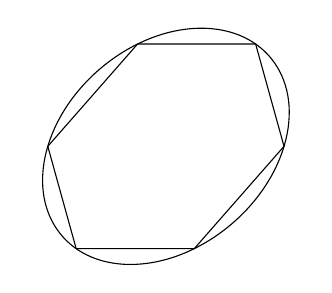
\begin{tikzpicture}[scale=1, font=\footnotesize, line join=round, line cap=round,>=stealth]
					\def \r{1.5};
					\begin{scope}[xslant=0.3]
						\foreach \i in {0,1,...,5}{
							\path (0,0)coordinate (O)--++(60*\i:\r) coordinate (A\i);}
						\draw (O) circle (\r);
						\draw (A0)--(A1)--(A2)--(A3)--(A4)--(A5)--cycle;
						%\foreach \p/\g in {A/0,B/-150,C/90} \fill[black] (\p) circle(1pt)+(\g:0.3) node{$\p$};
					\end{scope}
				\end{tikzpicture}
			\end{center}
		\end{enumerate}
	}
\end{bt}

% #768 | Archive/2024/TOAN_11_XE/TOAN_11_XE/data4/11C4/KNTT-4.3.tex | mã gốc 1T4K3-5
\begin{vd}%[Dự án Đề cương 11-Mui Doan]%[1T4K3-5]
	Cho hình chóp $S.ABCD$.  $M$, $N$ là hai điểm trên $AB$, $CD$. Mặt phẳng $(P)$ qua $MN$ và song song với $SA$.	Xác định thiết diện của $(P)$ với hình chóp.
	\loigiai{
		\immini{
			Mặt phẳng $(SAB)$ chứa đường thẳng $SA$ song song với mặt phẳng $(P)$ nên mặt phẳng $(SAB)$ cắt mặt phẳng $(P)$ theo giao tuyến song song với $SA$. Vẽ $MK\parallel SA$ ($K\in SB$) thì $MK$ là giao tuyến của $(P)$ với mặt phẳng $(SAB)$.\\
			Trong $(ABCD)$ ta có $AC\cap MN=E\Rightarrow E\in (P)$.\\
			Mặt phẳng $(SAC)$ chứa đường thẳng $SA$ song song với mặt phẳng $(P)$ nên mặt phẳng $(SAC)$ cắt mặt phẳng $(P)$ theo giao tuyến song song với $SA$. Vẽ $EH\parallel SA$ ($H\in SC$) thì $EH$ là giao tuyến của $(P)$ với mặt phẳng $(SAC)$.\\
			Khi đó giao tuyến của mặt phẳng $(SCD)$  với mặt phẳng $(P)$ là $NH$; $HK$ là giao tuyến của $(P)$ với $(SBC)$.\\
			Tứ giác $MNHK$  là thiết diện của $(P)$ với hình chóp $S.ABCD$.
		}
		{
			\begin{tikzpicture}[declare function={a=2.65;b=5;c=5;h=3;},line join=round]
				\path (0,0) coordinate (A)
				(-60:a) coordinate (B)
				(-35:c) coordinate (C)
				(b,0) coordinate (D)
				($(A)+(0.5,h)$) coordinate (S)
				($(A)!0.6!(B)$) coordinate (M)
				($(C)!0.7!(D)$) coordinate (N)
				($(S)!0.6!(B)$) coordinate (K)
				(intersection of A--C and M--N) coordinate (E)
				($(E)+(S)-(A)$) coordinate (x)
				(intersection of S--C and E--x) coordinate (H)
				;
				\fill [blue,opacity=0.3] (M)--(N)--(H)--(K);
				\draw[dashed] (A)--(D) (M)--(N) (A)--(C) (E)--(H);
				\draw (A)--(B)--(C)--(D)--(S)--(B) (S)--(A) (S)--(C) (N)--(H)--(K)--(M);
				\foreach \t/\g in {S/90,A/180,B/-90,C/-90,D/0,M/180,N/0,K/180,E/-90,H/90}{
					\draw[fill=black] (\t) circle (1pt) node[shift={(\g:7pt)},font=\scriptsize]{$ \t $};
				}
			\end{tikzpicture}
		}
	}
\end{vd}

% #769 | Archive/2024/TOAN_11_XE/TOAN_11_XE/data4/11C4/KNTT-4.3.tex | mã gốc 1T4K3-5
\begin{vd}%[Dự án Đề cương 11-Mui Doan]%[1T4K3-5]
	Cho hình chóp $S.ABCD$.  $M$, $N$ là hai điểm trên $SB$, $CD$. Mặt phẳng $(P)$ qua $MN$ và song song với $SC$.	Xác định thiết diện của $(P)$ với hình chóp.
	\loigiai{
		\immini{
			Mặt phẳng $(SBC)$ chứa đường thẳng $SC$ song song với mặt phẳng $(P)$ nên mặt phẳng $(SBC)$ cắt mặt phẳng $(P)$ theo giao tuyến song song với $SC$. Vẽ $MK\parallel SC$ ($K\in BC$) thì $MK$ là giao tuyến của $(P)$ với mặt phẳng $(SBC)$.\\
			Mặt phẳng $(SCD)$ chứa đường thẳng $SC$ song song với mặt phẳng $(P)$ nên mặt phẳng $(SCD)$ cắt mặt phẳng $(P)$ theo giao tuyến song song với $SC$. Vẽ $NP\parallel SC$ ($P\in SD$) thì $NP$ là giao tuyến của $(P)$ với mặt phẳng $(SCD)$.\\
			Trong $(ABCD)$ ta có $AC\cap NK=E\Rightarrow E\in (P)$.\\
			Mặt phẳng $(SAC)$ chứa đường thẳng $SC$ song song với mặt phẳng $(P)$ nên mặt phẳng $(SAC)$ cắt mặt phẳng $(P)$ theo giao tuyến song song với $SC$. Vẽ $EH\parallel SC$ ($H\in SA$) thì $EH$ là giao tuyến của $(P)$ với mặt phẳng $(SAC)$.\\
			Khi đó giao tuyến của mặt phẳng $(SAD)$  với mặt phẳng $(P)$ là $PH$; $HM$ là giao tuyến của $(P)$ với $(SAB)$.\\
			Vậy thiết diện của $(P)$ với hình chóp $S.ABCD$ là	ngũ giác $MKNPH$.
		}
		{
			\begin{tikzpicture}[declare function={a=2.65;b=5;c=5;h=3;},line join=round]
				\path (0,0) coordinate (A)
				(-60:a) coordinate (B)
				(-35:c) coordinate (C)
				(b,0) coordinate (D)
				($(A)+(0.5,h)$) coordinate (S)
				($(S)!0.4!(B)$) coordinate (M)
				($(C)!0.7!(D)$) coordinate (N)
				($(C)!0.4!(B)$) coordinate (K)
				($(S)!0.7!(D)$) coordinate (P)
				(intersection of A--C and N--K) coordinate (E)
				($(E)+(S)-(C)$) coordinate (x)
				(intersection of A--S and E--x) coordinate (H)
				;
				\fill [blue,opacity=0.3] (M)--(K)--(N)--(P)--(H);
				\draw[dashed] (A)--(D) (M)--(N) (A)--(C) (N)--(K) (E)--(H)--(P);
				\draw (A)--(B)--(C)--(D)--(S)--(B) (S)--(A) (S)--(C) (N)--(P) (H)--(M)--(K);
				\foreach \t/\g in {S/90,A/180,B/-90,C/-90,D/0,M/180,N/0,K/-90,P/90,E/0,H/180}{
					\draw[fill=black] (\t) circle (1pt) node[shift={(\g:7pt)},font=\scriptsize]{$ \t $};
				}
			\end{tikzpicture}	
		}	
	}
\end{vd}

% #770 | Archive/2024/TOAN_11_XE/TOAN_11_XE/data4/11C4/KNTT-4.3.tex | mã gốc 1T4K3-5
\begin{vd}%[Dự án Đề cương 11-Mui Doan]%[1T4K3-5]
	Cho tứ diện $ABCD$, điểm $E$ nẳm giữa hai điểm $A$ và $C$. Gọi $P$ là mặt phẳng qua $E$ và song song với hai đường thẳng $AB$, $CD$. Xác định các giao tuyến của $(P)$ và các mặt của tứ diện. Hình tạo bởi các giao tuyến là hình gì?
	\loigiai{
		\immini{
			Mặt phẳng $(ABC)$ chứa đường thẳng $AB$ song song với mặt phẳng $(P)$ nên mặt phẳng $(ABC)$ cắt mặt phẳng $(P)$ theo giao tuyến song song với $AB$. Vẽ $EF\parallel AB$ ($F\in BC$) thì $EF$ là giao tuyến của $(P)$ với mặt phẳng $(ABC)$.\\
			Hai mặt phẳng $(ACD)$ và $(BCD)$ cùng chứa đường thẳng $CD$ song song với mặt phẳng $(P)$ nên chúng cắt mặt phẳng $(P)$ theo giao tuyến song song với $CD$. Vẽ $EF$, $GH$ lần lượt là giao tuyến của mặt phẳng $(P)$ với hai mặt phẳng $(ACD)$ và $(BCD)$. Khi đó $GH$ là giao tuyến của $(P)$ với mặt phẳng $(ABD)$.\\
			Mặt phẳng $(ABD)$ chứa đường thẳng $AB$ song song với mặt phẳng $(P)$ nên giao tuyến $GH$ của $(ABD)$ và $(P)$ song song với $AB$. Tứ giác $EFGH$ có $EF\parallel GH$ (vì cùng song song với $AB$) và $EH\parallel FG$ (vì cùng song song với $CD$) nên nó là hình bình hành.
		}
		{
			\begin{tikzpicture}[declare function={a=2.65;b=4.5;h=3;},line join=round]
				\path (0,0) coordinate (B)
				(-60:a) coordinate (C)
				(b,0) coordinate (D)
				($(B)+(0.5,h)$) coordinate (A)
				($(A)!0.4!(C)$) coordinate (E)
				($(B)!0.4!(C)$) coordinate (F)
				($(B)!0.4!(D)$) coordinate (G)
				($(A)!0.4!(D)$) coordinate (H)
				;
				\fill [blue,opacity=0.3] (E)--(F)--(G)--(H);
				\draw[dashed] (B)--(D) (F)--(G)--(H);
				\draw (B)--(C)--(D) (B)--(A)--(C) (A)--(D) (F)--(E)--(H) ;
				\foreach \t/\g in {A/90,B/180,C/-90,D/0,E/180,F/180,G/-90,H/90}{
					\draw[fill=black] (\t) circle (1pt) node[shift={(\g:7pt)},font=\scriptsize]{$ \t $};
				}
			\end{tikzpicture}
		}
	}
\end{vd}

% #771 | Archive/2024/TOAN_11_XE/TOAN_11_XE/data4/11C4/KNTT-4.3.tex | mã gốc 1T4K3-5
\begin{vd}%[Dự án Đề cương 11-Mui Doan]%[1T4K3-5]
	Cho tứ diện $ABCD$. Gọi $I$, $J$ lần lượt là trung điểm của $AB$ và $CD$. Mặt phẳng $(P)$ đi qua một điểm $M$ trên đoạn $IJ$ và song song với $AB$ và $CD$. Xác định thiết diện của $(P)$ với tứ diện $ABCD$.
	\loigiai{
		\immini{
			Mặt phẳng $(ICD)$ chứa đường thẳng $CD$ song song với mặt phẳng $(P)$ nên mặt phẳng $(ICD)$ cắt mặt phẳng $(P)$ theo giao tuyến song song với $CD$. Qua $M$ vẽ $PQ\parallel CD$ ($P\in IC$; $Q\in ID$) thì $PQ$ là giao tuyến của $(P)$ với mặt phẳng $(ICD)$.\\
			Mặt phẳng $(ABC)$ chứa đường thẳng $AB$ song song với mặt phẳng $(P)$ nên mặt phẳng $(ABC)$ cắt mặt phẳng $(P)$ theo giao tuyến song song với $AB$. Qua $P$ vẽ $EF\parallel AB$ ($E\in BC$; $F\in AC$) thì $EF$ là giao tuyến của $(P)$ với mặt phẳng $(SCD)$.\\
			Mặt phẳng $(ACD)$ chứa đường thẳng $CD$ song song với mặt phẳng $(P)$ nên mặt phẳng $(ACD)$ cắt mặt phẳng $(P)$ theo giao tuyến song song với $CD$. Vẽ $FG\parallel CD$ ($G\in AD$) thì $FG$ là giao tuyến của $(P)$ với mặt phẳng~$(ACD)$.
		}
		{
			\begin{tikzpicture}[declare function={a=2.65;b=4.5;h=3;},line join=round]
				\path (0,0) coordinate (B)
				(-60:a) coordinate (C)
				(b,0) coordinate (D)
				($(B)+(0.5,h)$) coordinate (A)
				($(A)!0.5!(B)$) coordinate (I)
				($(D)!0.5!(C)$) coordinate (J)
				($(I)!0.5!(J)$) coordinate (M)
				($(M)+(D)-(J)$) coordinate (x)
				(intersection of I--C and M--x) coordinate (P)
				(intersection of I--D and M--x) coordinate (Q)
				($(P)+(B)-(I)$) coordinate (y)
				(intersection of A--C and P--y) coordinate (F)
				(intersection of B--C and P--y) coordinate (E)
				($(F)+(D)-(C)$) coordinate (z)
				(intersection of A--D and F--z) coordinate (G)
				(intersection of B--D and G--Q) coordinate (H)
				;
				\fill [blue,opacity=0.3] (E)--(F)--(G)--(H);
				\draw[dashed] (B)--(D) (I)--(J) (I)--(D) (P)--(Q) (E)--(H)--(G);
				\draw (B)--(C)--(D) (B)--(A)--(C) (A)--(D) (I)--(C) (E)--(F)--(G);
				\foreach \t/\g in {A/90,B/180,C/-90,D/0,I/180,J/-30,M/90,P/180,Q/30,E/180,F/160,G/90,H/-90}{
					\draw[fill=black] (\t) circle (1pt) node[shift={(\g:7pt)},font=\scriptsize]{$ \t $};
				}
			\end{tikzpicture}	
		}
		\noindent
		Mặt phẳng $(ABC)$ chứa đường thẳng $AB$ song song với mặt phẳng $(P)$ nên mặt phẳng $(BCD)$ cắt mặt phẳng $(P)$ theo giao tuyến song song với $CD$. Vẽ $EH\parallel CD$ ($H\in BD$) thì $EH$ là giao tuyến của $(P)$ với mặt phẳng~$(BCD)$.\\
		Khi đó giao tuyến của mặt phẳng $(ABD)$  với mặt phẳng $(P)$ là $GH$.\\
		Ta có $Q\in (ABD)\cap (P)\Rightarrow Q\in QH$; $EF\parallel GH$; $FG\parallel EH$.\\
		Vậy thiết diện của $(P)$ với tứ diện $ABCD$ là	hình bình hành $EFGH$.		
	}
\end{vd}

% #772 | Archive/2024/TOAN_11_XE/TOAN_11_XE/data4/11C4/KNTT-4.3.tex | mã gốc 1T4K3-5
\begin{vd}%[Dự án Đề cương 11-Mui Doan]%[1T4K3-5]
	Cho hình chóp $S.ABCD$ có đáy $ABCD$ là hình bình hành. Gọi $O$ là giao điểm của hai đường chéo hình bình hành. Một mặt phẳng $(P)$ qua $O$ đồng thời song song với $SA$ và $CD$. Tìm thiết diện tạo bởi $(P)$ và hình chóp.
	\loigiai{
		\immini{
			Mặt phẳng $(SAC)$ chứa đường thẳng $SA$ song song với mặt phẳng $(P)$ nên mặt phẳng $(SAC)$ cắt mặt phẳng $(P)$ theo giao tuyến song song với $SA$. Vẽ $OP\parallel SA$ ($P\in SC$) thì $OP$ là giao tuyến của $(P)$ với mặt phẳng $(SAC)$.\\
			Mặt phẳng $(ABCD)$ chứa đường thẳng $CD$ song song với mặt phẳng $(P)$ nên mặt phẳng $(ABCD)$ cắt mặt phẳng $(P)$ theo giao tuyến song song với $CD$. Qua $O$ vẽ $MN\parallel CD$ ($M\in AD$; $N\in BC$) thì $MN$ là giao tuyến của $(P)$ với mặt phẳng $(ABCD)$.
		}{
			\begin{tikzpicture}[declare function={a=2.2;c=5;h=3.7;D=45;},line join=round]
				%	c: cạnh DC
				%	a: cạnh DA
				%h: đường cao
				%D: góc D của đáy
				\path
				(0,0) coordinate (D)
				(D:a) coordinate (A)
				(c,0) coordinate (C)
				($(A)+(C)-(D)$) coordinate (B)
				($(A)+(70:h)$)  coordinate (S)
				($(S)!0.5!(C)$)  coordinate (P)
				($(A)!0.5!(C)$)  coordinate (O)
				($(A)!0.5!(D)$)  coordinate (M)
				($(B)!0.5!(C)$)  coordinate (N)
				($(P)+(D)-(C)$) coordinate (x)
				(intersection of P--x and S--D) coordinate (Q)
				;
				\fill [blue,opacity=0.3] (M)--(N)--(P)--(Q);
				\draw[dashed] (B)--(A)--(D)--cycle (S)--(A)--(C) (Q)--(M)--(N) (O)--(P);
				\draw (S)--(B)--(C)--(D)--cycle (S)--(C) (N)--(P)--(Q);
				\foreach \t/\g in {A/180,B/0,C/0,D/180,S/90,P/60,O/-90,M/-90,N/0,Q/180}{
					\draw[fill=black] (\t) circle (1pt) node[shift={(\g:7pt)},font=\scriptsize]{$ \t $};
				}
			\end{tikzpicture}
		}
		\noindent
		Mặt phẳng $(SCD)$ chứa đường thẳng $CD$ song song với mặt phẳng $(P)$ nên mặt phẳng $(SCD)$ cắt mặt phẳng $(P)$ theo giao tuyến song song với $CD$. Vẽ $PQ\parallel CD$ ($Q\in SD$) thì $PQ$ là giao tuyến của $(P)$ với mặt phẳng $(SCD)$.\\
		Ta có $NP$ là giao tuyến của mặt phẳng $(P)$ với $(SBC)$.\\
		Tứ giác $MPNQ$ có $MN\parallel PQ$ (vì cùng song song với $CD$)  nên nó là hình thang.	
	}
\end{vd}

% #773 | Archive/2024/TOAN_11_XE/TOAN_11_XE/data4/11C4/KNTT-4.3.tex | mã gốc 1C4T3-2
\begin{bt}%[Tex hóa SGK 11-CD]%[Phạm Tiến Long]%[1C4T3-2]
	Trong phòng học của lớp, hãy nêu những hình ảnh về đường thẳng song song với mặt phẳng.
	\loigiai{Nêu những hình ảnh trong phòng học gợi nên hình ảnh về đường thẳng song song với mặt phẳng, ví dụ: mép trên hoặc mép dưới của bảng song song với nền nhà, những cái trụ song song với những bức tường...}
\end{bt}

% #774 | Archive/2024/TOAN_11_XE/TOAN_11_XE/data4/11C4/KNTT-4.3.tex | mã gốc 1C4B2-2
\begin{bt}%[Tex hóa SGK 11-CD]%[Phạm Tiến Long]%[1C4B2-2]
%	\immini
%	{Trong hình bên, khi cắt bánh sinh nhật, mặt cắt và mặt khay đựng bánh lần lượt gợi nên hình ảnh mặt phẳng $(Q)$ và mặt phẳng $(P)$; mép trên và mép dưới của lát cắt lần lượt gợi nên hình ảnh hai đường thẳng $a$ và $b$ trong đó $a$ song song với mặt phẳng $(P)$. Cho biết hai đường thẳng $a$, $b$ có song song với nhau hay không.
%	}{	\begin{tikzpicture}[join=round,cap=round]
%			
%			\path
%			(-2.5,0) coordinate (A)
%			(2.5,0) coordinate (B)
%			(1.5,-1) coordinate (C)
%			($(A)+(C)-(B)$) coordinate (D)
%			;	
%			
%			\tkzMarkAngle[mark=](C,D,A)
%			\tkzLabelAngle[pos=0.5](C,D,A){$P$}
%			\draw (A)--(B)--(C)--(D)--(A);	
%			\def\a{1.4}
%			\def\b{0.5}
%			\def\h{.25}
%			\def\lat(#1,#2){
%				\begin{scope}[white,shift={(90:#1)}]
%					\path 
%					(0:0) coordinate (O)
%					(0:\a)  coordinate (A)
%					arc (360:240:{\a} and {\b}) coordinate (B')
%					(A) arc (0:60:{\a} and {\b}) coordinate (B)
%					(A) arc (0:120:{\a} and {\b}) coordinate (C)
%					(A) arc (0:-60:{\a} and {\b}) coordinate (C')
%					;
%					\draw [fill=#2] 
%					(O) rectangle ($(O)+(180:\a)+(270:\h)$)
%					(B') arc (240:360:{\a} and {\b}) --++(270:\h) arc (360:240:{\a} and {\b})--cycle
%					;
%					\draw [fill=#2] (O) -- (B') arc (-120:180:{\a} and {\b})--cycle;
%					\draw (A)--(O) (B)--(B') (C)--(C');
%					\begin{scope}[shift={(200:1)}]
%						\draw[fill=#2] (90:\h) --++(180:\a) --++(270:\h) arc (180:240:{\a} and {\b})--(0:0)--cycle;
%						\draw[fill=#2] (90:\h) --++(180:\a) arc (180:240:{\a} and {\b})--cycle;
%					\end{scope}
%				\end{scope}
%			}
%			
%			\lat(0,green)
%			\lat(\h,blue!50!white)
%			\lat(2*\h,brown)
%			\draw(-0.5,0.67)--(-2,-0.25)node[above]{$a$};
%			\draw[yshift=-21](-0.5,0.67)--(-2,-0.25)node[above]{$b$}
%			(-1.3,0.5)node{$Q$}
%			;
%		\end{tikzpicture}
%	}
%	\loigiai{Theo định lí 2 ta có hai đường thẳng $a$ và $b$ song song với nhau}
%\end{bt}

% #775 | Archive/2024/TOAN_11_XE/TOAN_11_XE/data4/11C4/KNTT-4.3.tex | mã gốc 1C4B3-2
\begin{bt}%[Tex hóa SGK 11-CD]%[Phạm Tiến Long]%[1C4B3-2]
	Cho tứ diện $ABCD$. Gọi $G$ là trọng tâm của tam giác $ABD$, điểm $I$ nằm trên cạnh $BC$ sao cho $BI=2IC$. Chứng minh rằng $IG$ song song với mặt phẳng $(ACD)$.
	\loigiai{
		\immini
		{
			Gọi $M$ là trung điểm của cạnh $AD$.\\
			Xét tam giác $BCM$ có $\dfrac{BI}{BC}=\dfrac{BG}{BM}=\dfrac{2}{3}\Rightarrow IG\parallel CM$.\\
			Mà $CM \subset (ACD)$ và $IG \not\subset (ACD)$ nên suy ra $IG \parallel (ACD)$.
		}
		{
			
			\begin{tikzpicture}[scale=0.7, font=\footnotesize, line join=round, line cap=round, >=stealth]
				\def\a{0}  \def\b{0} 
				\def\c{2}  \def\d{3} 
				\def\e{5}  \def\f{0} 
				\pgfmathsetmacro\g{\a/3+\c/3+\e/3}
				\pgfmathsetmacro\h{\b/3+\d/3+\f/3}
				\path
				(\a,\b) coordinate (B)
				(\c,\d) coordinate (A)
				(\e,\f) coordinate (D)
				(1.5,-2) coordinate (C)
				(\g,\h) coordinate (G)
				($(B)!2/3!(C)$) coordinate (I)
				($(A)!1/2!(D)$) coordinate (M)
				;
				\draw (A)--(D)--(C)--(B)--(A)--(C)--(M);
				\draw[dashed] (B)--(D) (I)--(G) (B)--(M);
				\foreach \x/\g in {A/90,B/180,C/270,D/0,I/250,G/90,M/45} \fill[black] (\x) circle (1pt)+(\g:0.3) node{$\x$};
			\end{tikzpicture}
		}
	}
\end{bt}

% #779 | Archive/2024/TOAN_11_XE/TOAN_11_XE/data4/11C4/KNTT-4.2.tex | mã gốc 1C4B2-2
\begin{bt}%[1C4B2-2]
	Quan sát phòng học của lớp và nêu lên hình ảnh của hai đường thẳng song song, cắt nhau, chéo nhau.
	\loigiai{Tùy theo tình hình thực tế lại lớp, chẳng hạn như hai mép cửa chính, lề bảng và mép tường,...}
\end{bt}

% #781 | Archive/2024/TOAN_11_XE/TOAN_11_XE/data4/11C4/KNTT-4.2.tex | mã gốc 1C4B2-3
\begin{bt}%[1C4B2-3]
	Cho hình chóp $S.ABCD$ có đáy $ABCD$ là hình bình hành. Gọi $M$, $N$, $P$ lần lượt là trung điểm của các cạnh $SA$, $AB$, $SD$. Xác định giao tuyến của mỗi cặp mặt phẳng sau: $(SAD)$ và $(SBC)$; $(MNP)$ và $(ABCD)$.
	\loigiai{
		\begin{itemize}
			\item 
			\immini{Xét hai mặt phẳng $(SAD)$ và $(SBC)$ có:\\
				$S$ là một điểm chung.\\
				Hơn nữa, ta có $\heva{&AD\parallel BC\\&AD\subset (SAD)\\&BC\subset (SBC)}$\\
				$\Rightarrow (SAD)\cap(SBC)=Sx\parallel AD$.}{\begin{tikzpicture}[scale=0.7, font=\footnotesize, line join=round, line cap=round, >=stealth]
					\coordinate[label=below:$A$] (A) at (0,0);
					\coordinate[label=below:$B$] (B) at (-1,-1.5);
					\coordinate[label=below:$D$] (D) at (5,0);
					\coordinate[label=right:$C$] (C) at ($(B)+(D)-(A)$);
					\coordinate[label=above:$S$] (S) at ($(A)+(1,3)$);
					\coordinate[label=left:$M$] (M) at ($(S)!0.5!(A)$);
					\coordinate[label=right:$P$] (P) at ($(S)!0.5!(D)$);	
					\coordinate[label=below:$N$] (N) at ($(A)!0.5!(B)$);
					\coordinate (Q) at ($(S)+(D)-(A)$);
					\coordinate (I) at ($(C)!0.5!(D)$);
					\draw (S)--(B) (S)--(C) (S)--(D) (B)--(C) (C)--(D);
					\draw [dashed] (S)--(A) (M)--(N) (N)--(P) (M)--(P) (N)--(I) (A)--(B) (A)--(D);
					\foreach \x in{A,B,C,D,S,M,N,P} \draw[fill=black] (\x) circle (1pt);
					\draw (S)--(Q) node[midway,below]{$x$};
					\draw [dashed] (N)--(I) node[midway,below]{$y$};
			\end{tikzpicture}}
			\item Xét hai mặt phẳng $(MNP)$ và $(ABCD)$ có:\\
			$N$ là một điểm chung.\\
			Hơn nữa ta có $\heva{&MP\parallel AD\quad(\text{vì}\, MP\, \text{là đường trung bình của tam giác}\, SAD)\\&AD\subset (ABCD)\\&MP\subset (MNP)}$\\
			$\Rightarrow (MNP)\cap(ABCD)=Ny\parallel AD$.
	\end{itemize}}
\end{bt}

% #782 | Archive/2024/TOAN_11_XE/TOAN_11_XE/data4/11C4/KNTT-4.2.tex | mã gốc 1C4B2-2
\begin{bt}%[1C4B2-2]
	Cho tứ diện $ABCD$. Gọi $G_1$, $G_2$ lần lượt là trọng tâm của các tam giác $ABC$ và $ABD$. Chứng minh rằng đường thẳng $G_1G_2$ song song với đường thẳng $CD$.
	\loigiai{
		\immini{Gọi $E$, $F$ lần lượt là trung điểm của $BC$ và $BD$.\\
			Ta có $G_1$ là trọng tâm tam giác $ABC$ nên $\dfrac{AG_1}{AE}=\dfrac{2}{3}$.\\
			$G_2$ là trọng tâm tam giác $ABD$ nên suy ra $\dfrac{AG_2}{AF}=\dfrac{2}{3}$.\\
			Xét tam giác $AEF$ có $\dfrac{AG_1}{AE}=\dfrac{AG_2}{AF}$. \\
			Theo định lí Ta-lét đảo ta có $G_1G_2\parallel EF$.}{\begin{tikzpicture}[scale=1, font=\footnotesize, line join=round, line cap=round, >=stealth]
				\coordinate[label=below:$B$] (B) at (0,0);
				\coordinate[label=right:$D$] (D) at (5,0);
				\coordinate[label=below:$C$] (C) at (3.5,-2);
				\coordinate (N) at ($(C)!0.5!(D)$);		
				\coordinate (O) at ($(B)!0.4!(N)$);
				\coordinate[label=above:$A$] (A) at ($(O)+(0,3)$);
				\coordinate[label=below:$E$] (E) at ($(B)!0.5!(C)$);
				\coordinate[label=below:$F$] (F) at ($(B)!0.5!(D)$);
				\coordinate[label=left:$G_1$] (G1) at ($(A)!2/3!(E)$);
				\coordinate[label=left:$G_2$] (G2) at ($(A)!2/3!(F)$);
				\draw (A)--(B)--(C)--(D)--cycle (A)--(C) (A)--(E);
				\draw [dashed] (B)--(D) (E)--(F) (G1)--(G2) (A)--(F);
				\foreach \x in{A,B,C,D,E,F,G1,G2} \draw[fill=black] (\x) circle (1pt);
		\end{tikzpicture}}
		
		
		
	}
\end{bt}

% #783 | Archive/2024/TOAN_11_XE/TOAN_11_XE/data4/11C4/KNTT-4.2.tex | mã gốc 1C4B2-2
\begin{bt}%[1C4B2-2]
	Cho hình chóp $S.ABCD$ có đáy $ABCD$ là hình thang với $AB$ là đáy lớn và $AB=2CD$. Gọi $M$, $N$ lần lượt là trung điểm của các cạnh $SA$ và $SB$. Chứng minh rằng đường thẳng $NC$ song song với đường thẳng $MD$.
	\loigiai{
		\immini{Ta có $MN$ là đường trung bình của tam giác $SAB$ nên $MN\parallel AB$ và $MN=\dfrac{1}{2}AB$.\hfill$(1)$\\
			Ta lại có $CD\parallel AB$ và $CD=\dfrac{1}{2}AB$.\hfill$(2)$\\
			Từ $(1)$ và $(2)$ ta có $MN\parallel CD$ và $MN=CD$.\\
			Vậy $MNCD$ là hình bình hành.\\
			Từ đó suy ra $MN\parallel NC$.}{\begin{tikzpicture}[scale=1, font=\footnotesize, line join=round, line cap=round, >=stealth]
				\coordinate[label=left:$A$] (A) at (0,0);
				\coordinate[label=right:$B$] (B) at (6,0);
				\coordinate[label=below:$C$] (C) at (4,-1.5);
				\coordinate (I) at ($(A)!0.5!(B)$);
				\coordinate[label=below:$D$] (D) at ($(A)+(C)-(I)$);
				\coordinate[label=above:$S$] (S) at ($(A)+(1,3)$);
				\coordinate[label=left:$M$] (M) at ($(S)!0.5!(A)$);
				\coordinate[label=right:$N$] (N) at ($(S)!0.5!(B)$);
				\draw (S)--(A) (S)--(B) (S)--(C) (S)--(D) (A)--(D)--(C)--(B) (M)--(D) (N)--(C);
				\draw [dashed] (A)--(B) (M)--(N);
				\foreach \x in {A,B,C,D,M,N,S} \draw[fill=black] (\x) circle (1pt);
	\end{tikzpicture}}}
\end{bt}

% #784 | Archive/2024/TOAN_11_XE/TOAN_11_XE/data4/11C4/KNTT-4.2.tex | mã gốc 1C4K2-2
\begin{bt}%[1C4K2-2]
	Cho hình chóp $S.ABCD$ có đáy $ABCD$ là hình bình hành. Gọi $M$, $N$, $P$, $Q$ lần lượt là trung điểm của các cạnh $AB$, $BC$, $CD$, $DA$; $I$, $J$, $K$, $L$ lần lượt là trung điểm của các đoạn thẳng $SM$, $SN$, $SP$, $SQ$.
	\begin{enumerate}
		\item Chứng minh rằng bốn điểm $I$, $J$, $K$, $L$ đồng phẳng và tứ giác $IJKL$ là hình bình hành.
		\item Chứng minh rằng $IK\parallel BC$.
		\item Xác định giao tuyến của hai mặt phẳng $(IJKL)$ và $(SBC)$.
	\end{enumerate}
	\loigiai{
		\begin{enumerate}
			\item \immini{Ta có $IJ$ là đường trung bình của tam giác $SMN$ nên $IJ\parallel MN$.\hfill$(1)$\\
				$KL$ là đường trung bình của tam giác $SPQ$ nên $KL\parallel PQ$.\hfill $(2)$\\
				Hơn nữa, $MN$ là đường trung bình của tam giác $ABC$ nên $MN\parallel AC$.\hfill$(3)$\\
				$PQ$ là đường trung bình của tam giác $ACD$ nên $PQ\parallel AC$.\hfill $(4)$\\
				Từ $(3)$ và $(4)$ suy ra $MN\parallel PQ$.\hfill$(5)$\\
				Từ $(1)$, $(2)$ và $(5)$ suy ra $IJ\parallel KL$.\\
				Suy ra bốn điểm $I$, $J$, $K$, $L$ đồng phẳng.}{\begin{tikzpicture}[scale=0.7, font=\footnotesize, line join=round, line cap=round, >=stealth]
					\coordinate[label=below:$A$] (A) at (0,0);
					\coordinate[label=below:$B$] (B) at (-1,-1.5);
					\coordinate[label=right:$D$] (D) at (5,0);
					\coordinate[label=right:$C$] (C) at ($(B)+(D)-(A)$);
					\coordinate[label=above:$S$] (S) at ($(A)+(1,3)$);
					\coordinate[label=left:$M$] (M) at ($(A)!0.5!(B)$);
					\coordinate[label=below:$N$] (N) at ($(B)!0.5!(C)$);
					\coordinate[label=right:$P$] (P) at ($(C)!0.5!(D)$);
					\coordinate[label=below:$Q$] (Q) at ($(A)!0.5!(D)$);
					\coordinate[label=left:$I$] (I) at ($(S)!0.5!(M)$);
					\coordinate[label=right:$K$] (K) at ($(S)!0.5!(P)$);
					\coordinate[label=below left:$J$] (J) at ($(S)!0.5!(N)$);
					\coordinate[label=above left:$L$] (L) at ($(S)!0.5!(Q)$);
					\coordinate (Z) at ($(S)!0.5!(B)$);
					\coordinate (W) at ($(S)!0.5!(C)$);	
					\draw (Z)--(W) node[below]{$x$};
					\draw (S)--(B) (S)--(C) (S)--(D) (B)--(C) (C)--(D) (S)--(N) (S)--(P);
					\draw [dashed] (S)--(A) (M)--(N)--(P)--(Q)--cycle (A)--(C) (I)--(J)--(K)--(L)--cycle (A)--(D) (A)--(B) (S)--(M) (S)--(Q) (I)--(K) (M)--(P);
					\foreach \x in{A,B,C,D,S,M,N,P,Q,I,J,K,L} \draw[fill=black] (\x) circle (1pt);
			\end{tikzpicture}}
			\item Ta có $IK$ là đường trung bình của tam giác $SMP$ nên suy ra $IK\parallel MP$.\hfill$(6)$\\
			Lại có $MP$ là đường trung bình của hình bình hành $ABCD$ nên suy ra $MP\parallel BC$.\hfill$(7)$\\
			Từ $(6)$ và $(7)$ suy ra $IK\parallel BC$.
			\item Xét hai mặt phẳng $(IJKL)$ và $(SBC)$ có:\\
			$J$ là một điểm chung.\\
			Hơn nữa, ta có\\
			$\heva{&IK\parallel BC\,(\text{chứng minh trên})\\&IK\subset (IJKL)\\&BC\subset (SBC)}$
			$\Rightarrow (IJKL)\cap (SBC)=Jx\parallel BC$.
	\end{enumerate}}
\end{bt}

% #785 | Archive/2024/TOAN_11_XE/TOAN_11_XE/data4/11C4/KNTT-4.2.tex | mã gốc 1C4K2-2
\begin{bt}%[1C4K2-2]
	Cho tứ diện $ABCD$. Gọi $I$, $J$ lần lượt là trung điểm của các cạnh $BC$, $CD$. Trên cạnh $AC$ lấy điểm $K$. Gọi $M$ là giao điểm của $BK$ và $AI$, $N$ là giao điểm của $DK$ và $AJ$. Chứng minh rằng đường thẳng $MN$ song song với đường thẳng $BD$.
	\loigiai{
		\immini{Xét $3$ mặt phẳng: $(BCD)$, $(AIJ)$ và $(KBD)$ có:\\
			$(BCD)\cap (AIJ)=IJ$, $(BCD)\cap(KBD)=BD$, $(AIJ)\cap(KBD)=MN$.\\
			Mà $IJ\parallel BD$ (vì $IJ$ là đường trung bình của tam giác $BCD$).\\
			Theo định lí về giao tuyến của ba mặt phẳng phân biệt cắt nhau đôi một, ta suy ra $MN\parallel BD$.}{\begin{tikzpicture}[scale=1, font=\footnotesize, line join=round, line cap=round, >=stealth]
				\coordinate[label=below:$B$] (B) at (0,0);
				\coordinate[label=right:$D$] (D) at (5,0);
				\coordinate[label=below:$C$] (C) at (3.5,-2);
				\coordinate[label=below:$I$] (I) at ($(B)!0.5!(C)$);		
				\coordinate[label=below:$J$] (J) at ($(C)!0.5!(D)$);
				\coordinate[label=above:$A$] (A) at ($(B)+(2,3)$);
				\coordinate[label=above left:$K$] (K) at ($(A)!0.3!(C)$);
				\path[name path=d] (D)--(K);
				\path[name path=b] (B)--(K);
				\path[name path=i] (I)--(A);
				\path[name path=j] (J)--(A);
				\path[name intersections={of=b and i}] (intersection-1) coordinate (M);
				\path[name intersections={of=d and j}] (intersection-1) coordinate (N);
				\draw (M) node[left] {$M$};
				\draw (N) node[right] {$N$};	
				\draw (A)--(B)--(C)--(D)--cycle (A)--(C) (A)--(I) (A)--(J) (K)--(B) (K)--(D);
				\draw [dashed] (B)--(D) (I)--(J) (M)--(N);
				\foreach \x in{A,B,C,D,I,J,M,N,K} \draw[fill=black] (\x) circle (1pt);
	\end{tikzpicture}}}
\end{bt}

% #787 | Archive/2024/TOAN_11_XE/TOAN_11_XE/data4/11C4/KNTT-4.1.tex | mã gốc 1K4Y0-1
\begin{vd}%[1K4Y0-1]
Có bao nhiêu đường thẳng đi qua hai điểm trong số ba điểm không thẳng hàng?
\loigiai{Qua hai điểm phân biệt có duy nhất một đường thẳng nên với ba điểm không thẳng hàng cho trước có ba đường thẳng đi qua hai điểm trong số ba điểm đó.}
\end{vd}

% #789 | Archive/2024/TOAN_11_XE/TOAN_11_XE/data4/11C4/KNTT-4.1.tex | mã gốc 1K4Y0-1
\begin{vd}%[1K4Y0-1]
	Có bao nhiêu mặt phẳng đi qua ba điểm thẳng hàng?
	\loigiai{Có vô số mặt phẳng đi qua ba điểm thẳng hàng.}
	\end{vd}

% #790 | Archive/2024/TOAN_11_XE/TOAN_11_XE/data4/11C4/KNTT-4.1.tex | mã gốc 1K4Y0-1
\begin{vd}%[1K4Y0-1]
 Cho bốn điểm $A$, $B$, $C$, $D$ không đồng phẳng. Có bao nhiêu mặt phẳng đi qua ba trong số bốn điểm đã cho?
 \loigiai{
 	\immini{
Có $4$ mặt phẳng đi qua ba trong số bốn điểm đã cho, đó là các mặt phẳng $(D A B)$, $(D A C)$, $(D B C)$ và $(A B C)$.
}{\begin{tikzpicture}[>=stealth,line join=round,line cap=round,font=\footnotesize,scale=0.8]
	
	\def \a{1} \def \b{-1} \def \c{4} \def \h{3.5}
	\path (.5,.5)coordinate(A) 
	+(\a,\b)coordinate(B)
	+(\c,0)coordinate(C)
	($(A)!2/3!($(B)!1/2!(C)$)$)coordinate(G) %tọa độ G là trọng tâm ABC
	+(0,\h)coordinate(S);
	
	%	\draw[ultra thin,color=gray] (-.5,-1.5) grid (5.5,4.5);
	\draw [dashed](A)--(C);
	\draw[thick] (S)--(A)--(B)--(S)--(C)--(B);
	
	\draw [fill=white] (S) circle (1pt)node[above]{$S$}
	(A) circle (1pt)node[left]{$A$}
	(B) circle (1pt)node[below]{$B$}
	(C) circle (1pt)node[right]{$C$};	
\end{tikzpicture}}}
\end{vd}

% #791 | Archive/2024/TOAN_11_XE/TOAN_11_XE/data4/11C4/KNTT-4.1.tex | mã gốc 1K4Y0-1
\begin{vd}%[1K4Y0-1] 
\immini{Cho tam giác $A B C$ và một điểm $M$ thuộc đường thẳng $B C$.
	\begin{enumerate}
\item  Điểm $M$ có thuộc mặt phẳng $(A B C)$ hay không?
\item  Đường thẳng $A M$ có nằm trong mặt phẳng $(A B C)$ hay không?
\end{enumerate}}{\begin{tikzpicture}[line join=round,line cap=round,font=\footnotesize,scale=0.8]
\coordinate (B) at (0,0);
\coordinate(A) at (2,3);
\coordinate(C) at (4,0);
\coordinate(M) at (6,0);
\draw (A)--(B)--(C)--cycle;
\draw[shorten <=-0.5cm,shorten >=-0.5cm] (B)--(M);
\foreach \i/\j in {A/90,B/-90,C/-90,M/-90}\fill[black] (\i) circle (1pt) ($(\i)+(\j:3mm)$)node{$\i$};
\end{tikzpicture}}
\loigiai{	
\begin{enumerate}
	\item Đường thẳng $B C$ có hai điểm phân biệt $B, C$ thuộc mặt phẳng $(A B C)$ nên đường thẳng $B C$ nằm trong mặt phẳng $(A B C)$. Vì $M$ thuộc đường thẳng $B C$ nên $M$ thuộc mặt phẳng $(A B C)$.
\item  Đường thẳng $A M$ có hai điểm phân biệt $A, M$ thuộc mặt phẳng
$(A B C)$ nên đường thẳng $AM$ nằm trong mặt phẳng $(A B C)$.
\end{enumerate}}
\end{vd}

% #792 | Archive/2024/TOAN_11_XE/TOAN_11_XE/data4/11C4/KNTT-4.1.tex | mã gốc 1K4B0-1
\begin{vd}%[1K4B0-1]
	Cho tam giác $A B C$ và một điểm $S$ không thuộc mặt phẳng $(A B C)$. Gọi $M$, $N$ lần lượt là trung điểm của các đoạn thẳng $AB$, $AC$.
	\begin{enumerate}
\item Chỉ ra một điểm chung của hai mặt phẳng $(SBN)$, $(SCM)$ và khác điểm $S$.
\item  Giao tuyến của hai mặt phẳng $(S B N)$ và $(S C M)$ có đi qua trọng tâm của tam giác $A B C$ hay không?
\end{enumerate}
\loigiai{
	\immini{
\begin{enumerate}
	\item Trong tam giác $A B C$, hai đường trung tuyến $B N$ và $C M$ cắt nhau tại trọng tâm $G$ của tam giác. Điểm $G$ thuộc $B N$ nên cũng thuộc mặt phẳng $(S B N)$. Điểm $G$ thuộc $C M$ nên cũng thuộc mặt phẳng $(S C M)$. Vậy $G$ là một điểm chung của hai mặt phẳng $(S B N)$ và $(S C M)$.
\item Vì $S$, $G$ là hai điểm chung của hai mặt phẳng $(S B N)$ và $(S C M)$ nên giao tuyến của hai mặt phẳng này là đường thẳng $S G$. Đường thẳng này đi qua trọng tâm $G$ của tam giác $A B C$.
\end{enumerate}}{\begin{tikzpicture}[line join=round,line cap=round,font=\footnotesize,scale=1]
\coordinate (B) at (0,0);
\coordinate(A) at (1,-1);
\coordinate(C) at (4,0);
\coordinate (N) at ($(A)!.5!(C)$);
\coordinate(M) at ($(A)!.5!(B)$);
\coordinate(G) at ($(B)!2/3!(N)$);
\coordinate(S) at ($(G)+(100:3)$);
\draw (B)--(A)--(C)--(S)--cycle (S)--(A) (S)--(M) (S)--(N);
\draw[dashed] (N)--(B)--(C) (G)--(S)(C)--(M);
\foreach \diem in {A,B,C,S,M,N} \fill (\diem) circle(1.0pt);
\foreach \i/\j in {A/-90, S/90,B/180,C/0,G/-80,M/-120,N/-120}\fill[black] (\i) circle (1pt) ($(\i)+(\j:3mm)$)node{$\i$}; 
\end{tikzpicture}}}
\end{vd}

% #793 | Archive/2024/TOAN_11_XE/TOAN_11_XE/data4/11C4/KNTT-4.1.tex | mã gốc 1K4B0-3
\begin{vd}%[1K4B0-3]
 Cho hai đường thẳng cắt nhau $a$, $ b$ và gọi $S$ là một điểm không thuộc mp$(a, b)$. Xác định giao tuyến của mp$(S, a)$ và mp$(S, b)$.
\loigiai{\immini{
Gọi $M$ là giao điểm của $a$ và $b$. Vì $M$ thuộc $a$ nên $M$ thuộc mp$(S, a)$. Vì $M$ thuộc $b$ nên $M$ thuộc mp$(S, b)$. Hai điểm $S$, $M$ cùng thuộc mp$(S, a)$ và mp$(S, b)$ nên giao tuyến của hai mặt phẳng đó là đường thẳng $SM$.}{\begin{tikzpicture}[scale=1, font=\footnotesize, line join=round, line cap=round,>=stealth]
	\path (0,0)coordinate (V) (4,0)
	 coordinate (X) (5.5,1.5) 
	 coordinate (Y) ($(V)+(Y)-(X)$)
	  coordinate (Z) (4.3,1) 
	  coordinate (A) (2.7,0.7)
	   coordinate (K) (2.0,1.2) 
		coordinate (H)--+(0.8,1.5) coordinate (S);
		\coordinate (C) at (1.8,1.2);
		 \coordinate (D) at (4,0.5);	
		 \coordinate (M) at (intersection cs:first line={(A)--(K)},second line={(C)--(D)});
		    
	\foreach \p in {V,X,Y,Z} {\path (\p)--+(0,-2) coordinate (\p');}
	\draw[fill=gray!20] (V)--(X)--(Y)--(Z)--cycle (S)--(M);
	\draw[shorten <=-0.5cm,shorten >=-1.5cm] (A)--(K) node[pos=1.8, below]{$a$};
	\draw(C)--(D) node[pos=0.2, above]{$b$};
		\foreach \p/\g in {M/-60,S/180} \fill[black] (\p) circle(1pt)+(\g:0.3) node{$\p$};
\end{tikzpicture}}}
\end{vd}

% #794 | Archive/2024/TOAN_11_XE/TOAN_11_XE/data4/11C4/KNTT-4.1.tex | mã gốc 1K4Y0-1
\begin{vd}%[1K4Y0-1]
	Cho hình chóp $S.ABCD$. Hỏi hình chóp có bao nhiêu đỉnh, bao nhiêu cạnh?
	\loigiai{\immini{Hình chóp $S.ABCD$ có $5$ đỉnh $S,\,A,\,B,\,C,\,D$ có $8$ cạnh $SA,\,SB,\,SC,\,SD,\,AB,\,BC,\,CD,\,DA$.}{	\begin{tikzpicture}[scale = 0.6, font=\footnotesize, line join = round, line cap = round,>=stealth]
				\def\a{5}
				\def\g{70}
				\def\b{4.5}
				\def\c{2}
				\def\d{4}
				\path (0,0) coordinate (A) --++(\a,0) coordinate (D)
				(A)--++(-\g:\c) coordinate (B)
				(A)--++(\g-10:\b) coordinate (S)
				(B)--++(-10:\c) coordinate (C)
				($(A)!0.5!(D)$) --++(0,-3) coordinate (x);
				\draw(S)--(A)--(B)--(C)--(D)--cycle (C)--(S)--(B);
				\draw[dashed] (A)--(D);
				\foreach \x/\g in {A/180,B/-90,C/-90,D/0,S/90} \fill[black] (\x) circle (1pt) ($(\x)+(\g:3mm)$) node{$\x$};
			
	\end{tikzpicture}}}
	\end{vd}

% #795 | Archive/2024/TOAN_11_XE/TOAN_11_XE/data4/11C4/KNTT-4.1.tex | mã gốc 1K4K0-5
\begin{vd}%[1K4K0-5]
	Cho tứ diện $ABCD$. Trên các đoạn $CA, CB, BD$ cho lần lươt các điểm $M, N, P$ sao cho $MN$ không song song với $AB$. Gọi $(\alpha)$ là mặt phẳng xác định bởi ba điểm $M, N, P$. Dựng thiết diện tạo bởi $(\alpha)$ và tứ diện $ABCD$.
	\loigiai{
		Ta có $M, N, P \in (\alpha) \Rightarrow (\alpha)\equiv(MNP)$.
		\begin{itemize}
			\item Ta có $(MNP) \cap (BCD)=MP$\hfill{(1)}
			\item Tương tự $(MNP) \cap (ABC)=MN$\hfill{(2)}
			\item Xét $(MNP)$ và $(ACD)$:\\
			\immini{$\heva{&N\in AC, AC \subset (ACD) \Rightarrow N \in (ACD)\\&N \in (MNP)} \Rightarrow N \in (ACD) \cap (MNP)$.\\
				Trong $(BCD)$, gọi $E=MP \cap CD$, ta có\\ $\heva{&E\in MP ,MP \subset (MNP) \Rightarrow E \in (MNP)\\&E\in CD,CD \subset (ACD) \Rightarrow E \in (ACD)} \Rightarrow E \in (MNP) \cap (ACD)$.\\
				Suy ra $(MNP) \cap (ACD)=NP$\hfill{(3)}}
			{\begin{tikzpicture}[scale=0.8, font=\footnotesize, line join=round, line cap=round, >=stealth]
					\def\ac{4} % cạnh AC
					\def\ab{2} % cạnh AB
					\def\h{4} % chiều cao
					\def\gocB{50} % góc A của đáy
					\coordinate[label=left:$B$] (B) at (0,0);
					\coordinate[label=right:$D$] (D) at (\ac,0);
					\coordinate[label=below left:$C$] (C) at (-\gocB:\ab);
					\coordinate[label=below left:$M$] (M) at ($(B)!1/3!(C)$);
					\coordinate[label=below:$P$] (P) at ($(B)!2/3!(D)$);
					\coordinate (I) at ($(B)!1/2!(M)$);
					\coordinate[label=above:$A$] (A) at ($(I)+(90:\h)$);
					\coordinate[label=below left:$N$] (N) at ($(A)!1/3!(C)$);
					\coordinate[label=below:$E$] (E) at ($(C)!3/2!(D)$);
					\coordinate[label=above right:$F$] (F) at ($(A)!3/5!(D)$);
					\fill[lightgray,opacity=0.9] (M)--(N)--(F)--(P)--cycle;
					\draw[thick] (B)--(C)--(D)--(A)--cycle (A)--(C) (C)--(E) (N)--(E) (M)--(N);
					\draw[thick][dashed] (M)--(B) (B)--(D) (M)--(E) (F)--(P);
					\foreach \diem in {B,A,C,M,P,E,N,F}	\fill (\diem)circle(1.0pt);
					
			\end{tikzpicture}}
			\item  Trong $(ACD)$, gọi $F=NE \cap AD$. Suy ra $(MNP) \cap (ACD)=NF$\hfill{(4)}\\
			Từ $(1),(2),(3),(4)$ ta có thiết diện tạo bởi $(\alpha)$ và tứ diện $ABCD$ là tứ giác $MNFP$.
		\end{itemize}
	}
\end{vd}

% #796 | Archive/2024/TOAN_11_XE/TOAN_11_XE/data4/11C4/KNTT-4.1.tex | mã gốc 1K4K0-5
\begin{vd}%[1K4K0-5]
	Cho hình chóp $S.ABC$. Trên cạnh $SA, SB$ lần lượt lấy $M, N$ sao cho $MN$ không song song với $AB$. Gọi $P$ là điểm thuộc miền trong tam giác $ABC$. Xác định thiết diện khi cắt hình chóp bởi mặt phẳng $(MNP)$.
	\loigiai{
		\immini{Ta có $MN=(MNP)\cap (SAB)$\hfill{(1)}\\
			Trong mp $(SAB)$: gọi $Q=MN\cap AB$.\\
			Trong mp $(ABCD)$	 kéo dài $QP$ cắt $CB$, $CA$ lần lượt tại $R, T$.\\
			Khi đó \begin{align*}
				&NR=(MNP)\cap (SBC)&\hfill{(2)}\\
				&RJ=(MNP)\cap (ABC)&\hfill{(3)}\\
				&TM=(MNP)\cap (SAC)&\hfill{(4)}
			\end{align*}
			Từ (1), (2), (3), (4) ta có thiết diện là tứ giác $MNRJ$.}
		{\begin{tikzpicture}[scale=1, font=\footnotesize, line join=round, line cap=round, >=stealth]
				\def\ac{4} % cạnh AC
				\def\ab{2} % cạnh AB
				\def\h{5} % chiều cao
				\def\gocA{50} % góc A của đáy
				\coordinate[label=left:$A$] (A) at (0,0);
				\coordinate[label=right:$C$] (C) at (\ac,0);
				\coordinate[label=below left:$B$] (B) at (-\gocA:\ab);
				\coordinate[label=below left:$Q$] (Q) at ($(A)!2!(B)$);
				\coordinate[label=above right:$J$] (J) at ($(C)!1/2!(A)$);
				\coordinate[label=above:$S$] (S) at ($(B)+(90:\h)$);
				\coordinate[label=left:$N$] (N) at ($(S)!2/3!(B)$);
				\coordinate[label=below right:$R$] (R) at ($(B)!1/3!(C)$);
				\coordinate[label=below left:$M$] (M) at ($(S)!1/2!(A)$);
				\coordinate[label=right:$P$] (P) at ($(J)!1/2!(R)$);
				\draw[thick] (S)--(A)--(B) (C)--(S) (S)--(B) (A)--(Q) (Q)--(R) (M)--(Q) (N)--(R)--(C);
				\draw[thick][dashed] (M)--(A)--(C) (M)--(J) (B)--(R)--(J) (M)--(P);
				\foreach \diem in {A,B,C,S,J,M,N,Q,R,P}	\fill (\diem)circle(1.0pt);
		\end{tikzpicture}}
	}
\end{vd}

% #797 | Archive/2024/TOAN_11_XE/TOAN_11_XE/data4/11C4/KNTT-4.1.tex | mã gốc 1K4K0-5
\begin{vd}%[1K4K0-5]
	Cho hình chóp $S.ABC$. Gọi $K, N$ lần lượt là trung điểm $SA, BC$ và $M$ là điểm thuộc đoạn $SC$ sao cho $3SM=2MC$.
	\begin{enumerate}
		\item Tìm thiết diện của $(KMN)$ và hình chóp.
		\item  Mặt phẳng $(KMN)$ cắt $AB$ tại $I$. Đặt $IA=kIB$. Tìm $k$.
	\end{enumerate}
	\loigiai{
		\begin{enumerate}
			\item Tìm thiết diện của $(KMN)$ và hình chóp.\\
			\immini{	$MN=(KMN)\cap (SBC)$\hfill{(1)}\\
				$MK=(KMN)\cap (SAC)$\hfill{(2)}\\
				Trong mp $(SAC)$ gọi $J=MK\cap AC$.\\
				Trong mp $(ABC)$ gọi $I=JN\cap AB$. Khi đó\\
				$KI=(KMN)\cap (SAB)$\hfill{(3)}\\
				$IN=(KMN)\cap (ABC)$\hfill{(4)}\\
				Từ (1), (2), (3), (4) ta có thiết diện là tứ giác $MNIK$.}
			{\begin{tikzpicture}[scale=1, font=\footnotesize, line join=round, line cap=round, >=stealth]
					\def\ac{3} % cạnh AC
					\def\ab{2} % cạnh AB
					\def\h{4} % chiều cao
					\def\gocA{50} % góc A của đáy
					\coordinate[label=above left:$A$] (A) at (0,0);
					\coordinate[label=right:$C$] (C) at (\ac,0);
					\coordinate[label=below left:$B$] (B) at (-\gocA:\ab);
					\coordinate[label=above:$S$] (S) at ($(B)+(90:\h)$);
					\coordinate[label=above right:$M$] (M) at ($(S)!2/5!(C)$);
					\coordinate[label=above left:$K$] (K) at ($(A)!1/2!(S)$);
					\coordinate[label=below:$N$] (N) at ($(B)!1/2!(C)$);
					\coordinate[label=below:$J$] (J) at ($(C)!3!(A)$);
					\coordinate[label=below:$I$] (I) at ($(A)!1/3!(B)$);
					\draw[thick] (I)--(B)--(C)--(S)--cycle (S)--(B) (M)--(N) (K)--(J)--(I) (S)--(K)--(I);
					\draw[thick][dashed] (I)--(A)--(C) (K)--(N) (M)--(K)--(A)--(J) (N)--(I);
					\foreach \diem in {A,B,C,S,M,N,K,J,I}	\fill (\diem)circle(1.0pt);
			\end{tikzpicture}}
			\item  Mặt phẳng $(KMN)$ cắt $AB$ tại $I$. Đặt $IA=kIB$. Tìm $k$.\\
			Ta có $3SM=2MC \Rightarrow SM=\dfrac{2}{3}MC=\dfrac{2}{3}(SC-SM) \Rightarrow \dfrac{5}{3} \Rightarrow SM=\dfrac{2}{5}SC$.\\
			Theo định lí Meneleus trong tam giác $SAC$: $\dfrac{MS}{MC}\cdot\dfrac{KS}{KA}\cdot\dfrac{JC}{JA}=1 \Rightarrow \dfrac{JA}{JC}=\dfrac{2}{3}$.\\
			Theo định lí Meneleus trong $\triangle ABC$: $\dfrac{NC}{NB}\cdot\dfrac{IB}{IA}\cdot\dfrac{JA}{JC}=1 \Rightarrow \dfrac{IB}{IA}=\dfrac{3}{2} \Rightarrow IA=\dfrac{2}{3}IB \Rightarrow k=\dfrac{2}{3}$.
		\end{enumerate}
	}
\end{vd}

% #798 | Archive/2024/TOAN_11_XE/TOAN_11_XE/data4/11C4/KNTT-4.1.tex | mã gốc 1K4K0-5
\begin{vd}%[1K4K0-5]
	Cho hình chóp $ABCD$. Trên cạnh $AB$ lấy điểm $M$, điểm $N$ trên $BC$ thỏa $BN=2NC$, $P$ là trung điểm $CD$. Xác định thiết diện khi cắt hình chóp bởi mặt phẳng $(MNP)$.
	\loigiai{
		\immini{Ta có $MN=(MNP)\cap (ABC)$\hfill{(1)}\\
			$NP=(MNP)\cap (BCD)$\hfill{(2)}\\
			Trong mặt phẳng $(BCD)$: gọi $I=NP\cap BD$.\\
			Trong mặt phẳng $(ABD)$: gọi $J=MI\cap AD \Rightarrow MJ=(MNP)\cap (ABD)$\hfill{(3)}\\
			$JP=(MNP)\cap (ACD)$\hfill{(4)}\\
			Từ (1), (2), (3), (4) ta có thiết diện là tứ giác $MNPJ$.}
		{\begin{tikzpicture}[line join=round, line cap=round,thick,scale=0.8]
				\tikzset{label style/.style={font=\footnotesize}}
				\coordinate[label=above left:$A$] (A) at (2,3);
				\coordinate[label=below left:$B$] (B) at (0,0);
				\coordinate[label=above right:$D$] (D) at (4,0);
				\coordinate[label=below:$C$] (C) at (1,-2);
				\coordinate[label=above left:$M$] (M) at ($(A)!1/2!(B)$);
				\coordinate[label=above left:$N$] (N) at ($(B)!2/3!(C)$);
				\coordinate[label=below right :$P$] (P) at ($(C)!1/2!(D)$);
				\draw[thick] (A)--(B)--(C)--(D)--cycle (M)--(N) (A)--(C);
				\draw[thick][dashed] (B)--(D) (M)--(P)--(N);
				\foreach \diem in {A,B,C,D,P,M,N}	\fill (\diem)circle(1.5pt);
		\end{tikzpicture}}
	}
\end{vd}

% #799 | Archive/2024/TOAN_11_XE/TOAN_11_XE/data4/11C4/KNTT-4.1.tex | mã gốc 1K4K0-5
\begin{vd}%[1K4K0-5] CHƯA GÁN ID
	Cho hình chóp $S.ABCD$ có đáy là hình thang đáy lớn $AD$. Lấy điểm $M$ trên  cạnh $SB$. Tìm thiết diện tạo bởi mặt phẳng $(AMD)$ và hình chóp.
	\loigiai{
		\immini{ Ta có $AM=(AMD)\cap (SAB)$\hfill{(1)}\\
			$AD=(AMD)\cap (ABCD)$\hfill{(2)}\\
			Trong mặt phẳng $(SBC)$, dựng đường thẳng qua $M$ song song $BC$ và cắt $SC$ tại $N\\
			\Rightarrow MN=(AMD)\cap (SAB)$, $ND=(AMD)\cap (SAB)$\hfill{(3)}\\
			Từ (1), (2), (3) ta có thiết diện là hình thang $ADNM$ (vì $MN\parallel BC\parallel AD$).}
		{\begin{tikzpicture}[scale=0.6,line join=round, line cap=round,thick]
				\tikzset{label style/.style={font=\footnotesize}}
				\coordinate[label=above left:$S$] (S) at (2.5,5);
				\coordinate[label=above left:$A$] (A) at (0,0);
				\coordinate[label=below left:$B$] (B) at (1,-2);
				\coordinate[label=above right:$D$] (D) at (6,0);
				\coordinate[label=below:$C$] (C) at (4,-2);
				\coordinate[label=above left:$M$] (M) at ($(S)!1/2!(B)$);
				\coordinate[label=above left:$N$] (N) at ($(S)!1/2!(C)$);
				\draw[thick] (A)--(B)--(C)--(D)--(S)--cycle (S)--(B) (S)--(C) (A)--(M)--(N)--(D);
				\draw[thick][dashed] (A)--(D) (M)--(D);
				\foreach \diem in {A,B,C,D,S,M,N}	\fill (\diem)circle(1.5pt);
		\end{tikzpicture}}
	}
\end{vd}

% #800 | Archive/2024/TOAN_11_XE/TOAN_11_XE/data4/11C4/KNTT-4.1.tex | mã gốc 1K4K0-6
\begin{vd}%[1K4K0-6]
	Cho tứ diện $SABC$. Trên các cạnh $SA$, $SB$, $SC$ lần lượt lấy các điểm $M$, $N$, $P$ sao cho
	$MN$ cắt $AB$ tại $I$, $NP$ cắt $BC$ tại $J$ và $MP$ cắt $AC$ tại $K$. Chứng minh rằng ba điểm
	$I$, $J$, $K$ thẳng hàng.
	\loigiai{ 
		\begin{center}
			\begin{tikzpicture}[scale=1, font=\footnotesize, line join=round, line cap=round, >=stealth]
				\path
				(0,0) coordinate (A)node[below]{$A$}
				($(A)+(-60:2.5)$) coordinate (B)node[below]{$B$}
				($(A)+(0:4)$) coordinate (C)node[right]{$C$}
				($(A)+(70:4)$) coordinate (S)node[right]{$S$}
				($(C)!2/3!(S)$) coordinate (P)node[above]{$P$}
				($(A)+(70:1.5)$) coordinate (M)node[right]{$M$}
				($(B)!1/5!(S)$) coordinate (N)node[right]{$N$}
				($(M)!2!180:(P)$)coordinate (Mt)
				($(A)!1!180:(C)$)coordinate (At)
				($(N)!2!180:(M)$)coordinate (Nt)
				($(B)!1!180:(A)$)coordinate (Bt)
				($(N)!1!180:(P)$)coordinate (Nt')
				($(B)!1!180:(C)$)coordinate (Bt')
				;
				\path[name path=a] (M)--(Mt);
				\path[name path=b] (A)--(At);
				\path [name intersections={of=a and b,by=K}];
				\path(K) coordinate (K)node[left]{$K$};
				\path[name path=c] (N)--(Nt);
				\path[name path=d] (B)--(Bt);
				\path [name intersections={of=c and d,by=I}];
				\path(I) coordinate (I)node[left]{$I$};
				\path[name path=e] (N)--(Nt');
				\path[name path=f] (B)--(Bt');
				\path [name intersections={of=e and f,by=J}];
				\path(J) coordinate (J)node[left]{$J$};
				\draw[thick](S)--(A)--(B)--(C)--(S)--(B) (M)--(K)--(A) (M)--(I)--(B) (P)--(J)--(B);
				\draw[thick][dashed](A)--(C) (P)--(M);
				\foreach\p in{P,M,N,K,I,J}\draw[thick][fill=black](\p)circle(1pt);
			\end{tikzpicture}
		\end{center}		
		Gọi đường thẳng $d$ là giao tuyến của hai mặt phẳng $(MNP)$ và $(ABC)$.\\
		Ta có $K=MP\cap AC \Rightarrow \heva{&K \in MP,MP\subset (MNP)\Rightarrow K\in(MNP)\\&K \in AC,AC\subset (ABC)\Rightarrow K\in(ABC)}\Rightarrow K\in d\quad (1)$\\
		Tương tự:\\
		$$I=MN\cap AB \Rightarrow \heva{&I \in MN,MN\subset (MNP)\Rightarrow I\in(MNP)\\&I \in AB,AB\subset (ABC)\Rightarrow I\in(ABC)}\Rightarrow I\in d\quad (2)$$
		$$J=NP\cap BC \Rightarrow \heva{&J \in NP,NP\subset (MNP)\Rightarrow J\in(MNP)\\&J \in BC,BC\subset (ABC)\Rightarrow J\in(ABC)}\Rightarrow J\in d\quad (3)$$
		Từ (1),(2),(3), suy ra $I$, $J$, $K$ cùng thuộc $d$ $\Rightarrow$ ba điểm $I$, $J$, $K$ thẳng hàng (đpcm).	
	}
\end{vd}

% #801 | Archive/2024/TOAN_11_XE/TOAN_11_XE/data4/11C4/KNTT-4.1.tex | mã gốc 1K4K0-6
\begin{vd}%[1K4K0-6]%[1H2B1-5]
	Cho tứ diện $ABCD$ có $G$ là trọng tâm tam giác $BCD$. Gọi $M$, $N$, $P$ lần lượt là trung
	điểm của các cạnh $AB$, $BC$, $CD$.
	\begin{enumerate}
		\item Xác định giao tuyến của $(ADN)$ và $(ABP)$.
		\item Gọi $I=AG\cap MP$ và $J=CM\cap AN$. Chứng minh $D$, $I$, $J$ thẳng hàng.
	\end{enumerate}	
	\loigiai{ 
		\begin{center}
			\begin{tikzpicture}[scale=1, font=\footnotesize, line join=round, line cap=round, >=stealth]
				\path
				(0,0) coordinate (B)node[left]{$B$}
				($(A)+(-60:2.5)$) coordinate (C)node[below]{$C$}
				($(A)+(0:4)$) coordinate (D)node[right]{$D$}
				($(B)!1/2!(C)$) coordinate (N)node[right]{$N$}
				($(C)!1/2!(D)$) coordinate (P)node[left]{$P$}
				($(B)!2/3!(P)$) coordinate (G)node[below]{$G$}
				($(G)+(90:4)$) coordinate (A)node[above]{$A$}
				($(A)!1/2!(B)$) coordinate (M)node[left]{$M$}
				;
				\path[name path=a] (M)--(C);
				\path[name path=b] (A)--(N);
				\path [name intersections={of=a and b,by=J}];
				\path(J) coordinate (J)node[left]{$J$};
				\path[name path=c] (A)--(G);
				\path[name path=d] (M)--(P);
				\path [name intersections={of=c and d,by=I}];
				\path(I) coordinate (I)node[left]{$I$};
				\draw[thick] (A)--(B)--(C)--(D)--(A)--(C) (A)--(N) (C)--(M)(A)--(P);
				\draw[thick][dashed](B)--(D)--(N) (B)--(P) (A)--(G) (M)--(P);
				\foreach\p in{A,B,C,D,M,N,P,G,I,J}\draw[thick][fill=black](\p)circle(1pt);
			\end{tikzpicture}
		\end{center}
		\begin{enumerate}
			\item Ta có $\heva{A\in(ADN)\\A\in(ABP)}\Rightarrow A\in(ADN)\cap(ABP)\quad (1)$\\
			Tương tự $$G=BP\cap DN\Rightarrow\heva{&G\in DN,DN\subset(ADN)\Rightarrow G\in(ADN)\\&G\in BP,BP\subset(ABP)\Rightarrow G\in(ABP)}\Rightarrow G\in(ADN)\cap(ABP)\quad (2)$$
			Từ $(1)$, $(2)$ suy ra $(ADN)\cap(ABP)=AG$.
			\item Gọi đường thẳng $d$ là giao tuyến của hai mặt phẳng $(DCM)$ và $(ADN)$.\\
			Ta có $\heva{D \in (DCM)\\D \in (ADN)}\Rightarrow D\in d\quad (1)$\\
			Tương tự:\\
			$$I=AG\cap MP \Rightarrow \heva{&I \in AG,AG\subset (ADN)\Rightarrow I\in(ADN)\\&I \in MP,MP\subset (DCM)\Rightarrow I\in(DCM)}\Rightarrow I\in d\quad (2)$$
			$$J=CM\cap AN \Rightarrow \heva{&J \in CM,CM\subset (DCM)\Rightarrow J\in(DCM)\\&J \in AN,AN\subset (ADN)\Rightarrow J\in(ADN)}\Rightarrow J\in d\quad (3)$$
			Từ (1),(2),(3), suy ra $D$, $I$, $J$ cùng thuộc $d$ $\Rightarrow$ ba điểm $D$, $I$, $J$ thẳng hàng (đpcm).
		\end{enumerate}	
	}
\end{vd}

% #802 | Archive/2024/TOAN_11_XE/TOAN_11_XE/data4/11C4/KNTT-4.1.tex | mã gốc 1K4K0-6
\begin{vd}%[1K4K0-6]%[1H2K1-5]
	Cho hình chóp $S.ABCD$ có đáy $ABCD$ là hình bình hành tâm $O$, hai điểm $M$, $N$ lần lượt
	là trung điểm của $SB$, $SD$, điểm $P$ thuộc $SC$ và không là trung điểm của $SC$.
	\begin{enumerate}
		\item Tìm giao điểm của $SO$ với $(MNP)$.
		\item Tìm giao điểm $Q$ của $SA$ với mặt phẳng $(MNP)$.
		\item Gọi $F$, $G$, $H$ lần lượt là giao điểm của $QM$ và $AB$, $QP$ và $AC$, $QN$ và $AD$. Chứng
		minh ba điểm $F$, $G$, $H$ thẳng hàng.
	\end{enumerate}	
	\loigiai{ 
		\begin{center}
			\begin{tikzpicture}[scale=1, font=\footnotesize, line join=round, line cap=round, >=stealth]
				\path
				(0,0) coordinate (A)node[left]{$A$}
				($(A)+(-120:2)$) coordinate (B)node[left]{$B$}
				($(B)+(0:4)$) coordinate (C)node[below]{$C$}
				($(A)+(0:4)$) coordinate (D)node[left]{$D$}
				($(B)+(85:5)$) coordinate (S)node[left]{$S$}
				($(S)!1/2!(B)$) coordinate (M)node[left]{$M$}
				($(S)!1/2!(D)$) coordinate (N)node[above]{$N$}
				($(C)!1/4!(S)$) coordinate (P)node[right]{$P$}
				;
				\path[name path=a] (A)--(C);
				\path[name path=b] (B)--(D);
				\path [name intersections={of=a and b,by=O}];
				\path(O) coordinate (O)node[left]{$O$};
				\path[name path=c] (M)--(N);
				\path[name path=d] (S)--(O);
				\path [name intersections={of=c and d,by=I}];
				\path(I) coordinate (I)node[left]{$I$};
				\path
				($(I)!1!180:(P)$)coordinate (It)
				;
				\path[name path=e] (I)--(It);
				\path[name path=f] (S)--(A);
				\path [name intersections={of=e and f,by=Q}];
				\path(Q) coordinate (Q)node[left]{$Q$};
				\path
				($(N)!5!-180:(Q)$)coordinate (Nt)
				($(D)!3!-180:(A)$)coordinate (Dt)
				($(P)!2!-180:(Q)$)coordinate (Pt)
				($(C)!2!-180:(A)$)coordinate (Ct)
				($(M)!5!-180:(Q)$)coordinate (Mt)
				($(B)!3!-180:(A)$)coordinate (Bt)
				;
				\path[name path=g] (N)--(Nt);
				\path[name path=h] (D)--(Dt);
				\path [name intersections={of=g and h,by=F}];
				\path(F) coordinate (F)node[above]{$F$};
				\path[name path=i] (P)--(Pt);
				\path[name path=k] (C)--(Ct);
				\path [name intersections={of=i and k,by=G}];
				\path(G) coordinate (G)node[below]{$G$};
				\path[name path=u] (M)--(Mt);
				\path[name path=v] (B)--(Bt);
				\path [name intersections={of=u and v,by=H}];
				\path(H) coordinate (H)node[left]{$H$};
				\draw[thick](S)--(B)--(C)--(D)--(S)--(C) (M)--(P)--(N)--(F)--(D) (P)--(G)--(C) (M)--(H)--(B);
				\draw[thick][dashed](S)--(A)--(B) (A)--(D) (A)--(C) (B)--(D) (M)--(N) (S)--(O) (P)--(I)--(Q)--(M) (Q)--(N);
				\foreach\p in{A,B,C,D,S,M,N,P,O,I,Q,F,G,H}\draw[thick][fill=black](\p)circle(1pt);
			\end{tikzpicture}
		\end{center}
		\begin{enumerate}
			\item Trong $(SBD)$ ta có $\heva{&SO\cap MN=\{I\}\\&MN\subset(MNP)}\Rightarrow SO\cap(MNP)=\{I\}$.
			\item Chọn $mp(SAC)$ chứa $SA$.
			Ta có $(SAC)\cap(MNP)=PI$. Kẻ $PI\cap SA=\{Q\}$.\\
			Suy ra $SA\cap(MNP)=\{Q\}$.
			\item Gọi đường thẳng $d$ là giao tuyến của hai mặt phẳng $(MNPQ)$ và $(ABCD)$.\\
			Ta có 
			$$F=QM\cap AB \Rightarrow \heva{&F \in QM,QM\subset (MNPQ)\Rightarrow F\in(MNPQ)\\&F \in AB,AB\subset (ABCD)\Rightarrow F\in(ABCD)}\Rightarrow F\in d\quad (1)$$
			$$G=PQ\cap AC \Rightarrow \heva{&G \in PQ,PQ\subset (MNPQ)\Rightarrow G\in(MNPQ)\\&G \in AC,AC\subset (ABCD)\Rightarrow G\in(ABCD)}\Rightarrow G\in d\quad (2)$$
			$$H=NQ\cap AD \Rightarrow \heva{&H \in NQ,NQ\subset (MNPQ)\Rightarrow H\in(MNPQ)\\&H \in AD,AD\subset (ABCD)\Rightarrow H\in(ABCD)}\Rightarrow H\in d\quad (3)$$
			Từ (1),(2),(3), suy ra $F$, $G$, $H$ cùng thuộc $d$ $\Rightarrow$ ba điểm $F$, $G$, $H$ thẳng hàng (đpcm).
		\end{enumerate}	
	}
\end{vd}

% #803 | Archive/2024/TOAN_11_XE/TOAN_11_XE/data4/11C4/KNTT-4.1.tex | mã gốc 1K4K0-6
\begin{vd}%[1K4K0-6]%[1H2B1-5]
	Cho hình chóp $S.ABCD$ có $AD$ không song song với $BC$. Lấy $M$ thuộc $SB$ và $O$ là
	giao điểm $AC$ với $BD$.
	\begin{enumerate}
		\item Tìm giao điểm $N$ của $SC$ với $(ADM)$.
		\item Gọi $I=AN\cap DM$. Chứng minh $S$, $I$, $O$ thẳng hàng.
	\end{enumerate}
	\loigiai{ 
		\immini{
			\begin{enumerate}
				\item Chọn $mp(SBC)$ chứa $SC$. Gọi $H=AD\cap BC$.\\
				Ta có $(SBC)\cap(ADM)=MH$. Kẻ $MH\cap SC=N$.
				Suy ra $SC\cap(ADM)=N$.	
				\item Gọi đường thẳng $d$ là giao tuyến của hai mặt phẳng $(SAC)$ và $(SBD)$.\\
				Ta có 
				$\heva{&S\in(SAC)\\&S\in(SBD)}\Rightarrow S\in d\quad (1)$.\\
				Tương tự
				$$I=AN\cap SO \Rightarrow \heva{I \in AN,AN\subset (SAC)\Rightarrow I\in(SAC)\\I \in SO,SO\subset (SBD)\Rightarrow I\in(SBD)}\Rightarrow I\in d\quad (2)$$
				$$O=AC\cap BD \Rightarrow \heva{&O \in AC,AC\subset (SAC)\Rightarrow O\in(SAC)\\&O \in BD,BD\subset (SBD)\Rightarrow O\in(SBD)}\Rightarrow O\in d\quad (3)$$
				Từ (1),(2),(3), suy ra $S$, $I$, $O$ cùng thuộc $d$ $\Rightarrow$ ba điểm $S$, $I$, $O$ thẳng hàng (đpcm).
		\end{enumerate}}{\begin{tikzpicture}[scale=0.8, font=\footnotesize, line join=round, line cap=round, >=stealth]
				\path
				(0,0) coordinate (A)node[left]{$A$}
				($(A)+(0:4)$) coordinate (B)node[right]{$B$}
				($(A)+(-40:4)$) coordinate (C)node[below]{$C$}
				($(A)+(-60:2)$) coordinate (D)node[left]{$D$}
				($(A)+(80:4)$) coordinate (S)node[left]{$S$}
				($(B)!1/4!(S)$) coordinate (M)node[right]{$M$}
				($(D)!2!180:(A)$) coordinate (Dt)
				($(C)!2!180:(B)$) coordinate (Ct)
				;
				\path[name path=a] (A)--(C);
				\path[name path=b] (B)--(D);
				\path [name intersections={of=a and b,by=O}];
				\path(O) coordinate (O)node[below]{$O$};
				\path[name path=c] (D)--(Dt);
				\path[name path=d] (C)--(Ct);
				\path [name intersections={of=c and d,by=H}];
				\path(H) coordinate (H)node[left]{$H$};
				\path[name path=e] (S)--(C);
				\path[name path=f] (M)--(H);
				\path [name intersections={of=e and f,by=N}];
				\path(N) coordinate (N)node[left]{$N$};
				\path[name path=g] (A)--(N);
				\path[name path=h] (D)--(M);
				\path [name intersections={of=g and h,by=I}];
				\path(I) coordinate (I)node[above]{$I$};
				\draw[thick] (S)--(A)--(D)(C)--(B)--(S)--(D) (S)--(C)--(H)--(D) (M)--(H);
				\draw[thick][dashed](A)--(B) (A)--(C) (B)--(D)--(C) (A)--(M)--(D) (A)--(N);
				\foreach\p in{A,B,C,D,S,M,O,H,N,I}\draw[thick][fill=black](\p)circle(1pt);
		\end{tikzpicture}}
	}
\end{vd}

% #804 | Archive/2024/TOAN_11_XE/TOAN_11_XE/data4/11C4/KNTT-4.1.tex | mã gốc 1K4K0-6
\begin{vd}%[1K4K0-6]%[1H2B1-5]
	Cho tứ diện $ABCD$ có $G$ là trọng tâm tam giác $BCD$. Gọi $M$, $N$, $P$ lần lượt là trung
	điểm của $AB$, $BC$, $CD$.
	\begin{enumerate}
		\item Tìm giao tuyến của $(ADN)$ và $(ABP)$.
		\item Gọi $I=AG\cap MP$ và $J=CM\cap AN$ Chứng minh $D$, $I$, $J$ thẳng hàng.
	\end{enumerate}
	\loigiai{ 
		\begin{center}
			\begin{tikzpicture}[scale=1, font=\footnotesize, line join=round, line cap=round, >=stealth]
				\path
				(0,0) coordinate (B)node[left]{$B$}
				($(A)+(-60:2.5)$) coordinate (C)node[below]{$C$}
				($(A)+(0:4)$) coordinate (D)node[right]{$D$}
				($(B)!1/2!(C)$) coordinate (N)node[right]{$N$}
				($(C)!1/2!(D)$) coordinate (P)node[left]{$P$}
				($(B)!2/3!(P)$) coordinate (G)node[below]{$G$}
				($(G)+(90:4)$) coordinate (A)node[above]{$A$}
				($(A)!1/2!(B)$) coordinate (M)node[left]{$M$}
				;
				\path[name path=a] (M)--(C);
				\path[name path=b] (A)--(N);
				\path [name intersections={of=a and b,by=J}];
				\path(J) coordinate (J)node[left]{$J$};
				\path[name path=c] (A)--(G);
				\path[name path=d] (M)--(P);
				\path [name intersections={of=c and d,by=I}];
				\path(I) coordinate (I)node[left]{$I$};
				\draw[thick] (A)--(B)--(C)--(D)--(A)--(C) (A)--(N) (C)--(M)(A)--(P);
				\draw[thick][dashed](B)--(D)--(N) (B)--(P) (A)--(G) (M)--(P);
				\foreach\p in{A,B,C,D,M,N,P,G,I,J}\draw[thick][fill=black](\p)circle(1pt);
			\end{tikzpicture}
		\end{center}
		\begin{enumerate}
			\item Ta có 
			$\heva{&A\in(ADN)\\&A\in(ABP)}\Rightarrow A\in (ADN)\cap (ABP) \quad (1)$.\\
			Tương tự
			$$G=BP\cap DN \Rightarrow \heva{&G \in BP,BP\subset (ABP)\Rightarrow G\in(ABP)\\&G \in DN,DN\subset (ADN)\Rightarrow G\in(ADN)}\Rightarrow G\in(ADN)\cap (ABP) \quad (2)$$
			Từ $(1)$, $(2)$ $\Rightarrow (ADN)\cap (ABP)=AG$.
			\item Gọi đường thẳng $d$ là giao tuyến của hai mặt phẳng $(DMC)$ và $(ADN)$.\\
			Ta có 
			$\heva{&D\in(DMC)\\&D\in(ADN)}\Rightarrow D\in d\quad (1)$.\\
			Tương tự
			$$I=AG\cap MP \Rightarrow \heva{&I \in AG,AG\subset (ADN)\Rightarrow I\in(ADN)\\&I \in MP,MP\subset (DMC)\Rightarrow I\in(DMC)}\Rightarrow I\in d\quad (2)$$
			$$J=CM\cap AN \Rightarrow \heva{&J \in CM,CM\subset (DMC)\Rightarrow J\in(DMC)\\&J \in AN,AN\subset (ADN)\Rightarrow J\in(ADN)}\Rightarrow J\in d\quad (3)$$
			Từ (1),(2),(3), suy ra $D$, $I$, $J$ cùng thuộc $d$ $\Rightarrow$ ba điểm $D$, $I$, $J$ thẳng hàng (đpcm).
		\end{enumerate}	
	}
\end{vd}

% #805 | Archive/2024/TOAN_11_XE/TOAN_11_XE/data4/11C4/KNTT-4.1.tex | mã gốc 1K4G0-6
\begin{vd}%[1K4G0-6]
	Cho hình chóp $S.ABCD$ có $AB$ không song song $CD$. Gọi $M$ là trung điểm $SC$ và $O$ là giao điểm $AC$ với $BD$.
	\begin{enumerate}
		\item Tìm giao điểm $N$ của $SD$ với $(MAB)$.
		\item Chứng minh ba đường thẳng $SO, AM, BN$ đồng quy.
	\end{enumerate}
	\loigiai{
		\begin{enumerate}
			\item Tìm giao điểm $N$ của $SD$ với $(MAB)$.\\
			\immini{
				\begin{itemize}
					\item Chọn mặt phẳng phụ $(SCD)$ chứa $SD$.\\
					Xét $(SCD)$ và $(MAB)$:
					\item Trong $(ABCD)$, gọi $E = AB \cap CD$.\\
					Ta có: $\heva{&E \in AB, AB \subset(ABM) \Rightarrow E \in(ABM) \\ 
						&E \in CD, CD \subset(SCD) \Rightarrow E \in(SCD)}$\\
					$\Rightarrow E \in(ABM) \cap(SCD)$ \quad\quad $(1)$
					\item Mà $\heva{&M \in(ABM) \\ &M \in SC, SC \subset(SCD) \Rightarrow M \in(SCD)}$\\
					$\Rightarrow M \in(ABM) \cap (SCD)$.\quad\quad $(2)$\\
					Từ $(1),(2) \Rightarrow(ABM) \cap (SCD)= EM$.
					\item Trong $(SCD)$, gọi $N=SD \cap EM$.\\ Khi đó:
					$\heva{&N \in SD \\ &N \in EM, EM \subset(ABM)}$\\ 
					$\Rightarrow N = SD \cap (ABM)$.
			\end{itemize}}{
				\begin{tikzpicture}[scale=0.6, font=\footnotesize, line join=round, line cap=round, >=stealth]
					\coordinate[label=left:$A$] (A) at (-3,0);
					\coordinate[label=left:$B$] (B) at (-2,-2);
					\coordinate[label=below:$C$] (C) at (2,-4);
					\coordinate[label=right:$D$] (D) at (4,0);
					\coordinate[label=above:$S$] (S) at (0,6);
					%\coordinate (F) at (-3,3);
					\coordinate[label=right:$M$] (M) at ($(S)!1/2!(C)$);
					%\coordinate (N) at ($(E)!1/3!(A)$);
					%\coordinate (K) at ($(C)!1/3!(A)$);
					\draw[thick] (A)--(B) (C)--(D)--(S)--(A);
					\draw[thick] (B)--(S)--(C);
					\draw[thick] (S)--(D);
					\draw[thick][dashed] (B)--(C)--(A) (A)--(D);
					\draw[thick][dashed] (B)--(D) (A)--(M);
					\coordinate[label=below:$O$](O) at (intersection of A--C and B--D); %giao điểm
					\coordinate[label=below:$E$](E) at (intersection of A--B and C--D); %giao điểm
					\draw[thick] (E)--(B) (E)--(C);
					\coordinate[label=right:$N$](N) at (intersection of E--M and S--D); %giao điểm
					\draw[thick] (E)--(N);
					\draw[thick][dashed] (S)--(O) (B)--(N);
					\coordinate[label=above left :$I$](I) at (intersection of A--M and S--O); %giao điểm
					\foreach \diem in {A,B,C,D,N,M,E,O,S,I}	\fill (\diem)circle(1.5pt);
			\end{tikzpicture}}
			\item Chứng minh ba đường thẳng $SO, AM, BN$ đồng quy.
			\begin{note}
				$AM \subset (SAC), BN \subset (SBD)$ nên ta quan tâm đến hai mặt phẳng này.
			\end{note}
			Xét $(SAC)$ và $(SBD)$ có:
			\begin{itemize}
				\item $S \in(SAC) \cap (SBD) \quad\quad\quad\quad (3)$
				\item Ta có: $\heva{&O \in AC, AC \subset (SAC) \Rightarrow O \in(SAC) \\ 
					&O \in BD, BD \subset(SBD) \Rightarrow O \in(SBD)} \Rightarrow O \in (SAC) \cap (SBD)$ $\quad (4)$\\
				Từ $(3),(4) \Rightarrow(SAC) \cap(SBD)=SO.$
				\item Mặt khác, trong $(ABM),$ gọi $I= AM \cap BN$.\\
				$\heva{&I \in AM \subset(SAC) \\ &I \in BN \subset(SBD)} \Rightarrow I \in(SAC) \cap(SBD) \Rightarrow I \in SO.$
			\end{itemize}
			Do đó $SO, AM, BN$ đồng quy.
		\end{enumerate}
	}
\end{vd}

% #806 | Archive/2024/TOAN_11_XE/TOAN_11_XE/data4/11C4/KNTT-4.1.tex | mã gốc 1K4G0-6
\begin{vd}%[1K4G0-6]
	Cho hình chóp $S.ABCD$ có đáy $ABCD$ là tứ giác lồi. Lấy $M$ trên cạnh $SC$. Gọi $N$ là giao điểm của $SB$ và $(ADM)$. Gọi $O$ là giao điểm $AC$ và $BD$. Chứng minh rằng $SO, AM, DN$ đồng qui.
	\loigiai{
		\begin{itemize}
			\item Tìm $N$ là giao điểm của $SB$ và $(ADM)$.
			\immini{
				\begin{itemize}
					\item Chọn mặt phẳng phụ $(SBC)$ chứa $SB$.\\
					Xét $(SBC)$ và $(ADM)$:
					\item Trong $(ABCD)$, gọi $E = AD \cap BC$.\\
					Ta có: $\heva{&E \in BC, BC \subset(SBC) \Rightarrow E \in(SBC) \\ 
						&E \in AD, AD \subset(ADM) \Rightarrow E \in(ADM)}$\\
					$\Rightarrow E \in(SBC) \cap (ADM)$ \quad\quad $(1)$
					\item Mà $\heva{&M \in(ADM) \\ &M \in SC, SC \subset(SBC) \Rightarrow M \in (SBC)}$\\
					$\Rightarrow M \in(SBC) \cap (ADM)$.\quad\quad $(2)$\\
					Từ $(1),(2) \Rightarrow(SBC) \cap (ADM)= EM$.
					\item Trong $(SBC)$, gọi $N= SB \cap EM$.\\ Khi đó:
					$\heva{&N \in SB \\ &N \in EM, EM \subset(ADM)}$\\ 
					$\Rightarrow N = SB \cap (ADM)$.
			\end{itemize}}{
				\begin{tikzpicture}[scale=0.6, font=\footnotesize, line join=round, line cap=round, >=stealth]
					\coordinate[label=below left:$A$] (A) at (-3,0);
					\coordinate[label=left:$B$] (B) at (-2,-2);
					\coordinate[label=below:$C$] (C) at (2,-4);
					\coordinate[label=right:$D$] (D) at (4,0);
					\coordinate[label=above:$S$] (S) at (0,6);
					\coordinate[label=above right:$M$] (M) at ($(S)!1/2!(C)$);
					\coordinate[label=below:$O$](O) at (intersection of A--C and B--D); %giao điểm
					\coordinate[label=below:$E$](E) at (intersection of A--D and B--C); %giao điểm
					\coordinate[label=above left:$N$](N) at (intersection of S--B and M--E); %giao điểm
					\coordinate[label=below right:$I$](I) at (intersection of S--O and M--A); %giao điểm
					\draw[thick] (C)--(D)--(S);
					\draw[thick] (B)--(S)--(C) (M)--(E);
					\draw[thick] (C)--(E)--(S)--(D)--(M);
					\draw[thick][dashed] (S)--(A) (A)--(B) (C)--(A)--(E) (M)--(A)--(D);
					\draw[thick][dashed] (B)--(D) (S)--(O);
					\foreach \diem in {A,B,C,D,M,E,N,O,I}	\fill (\diem)circle(1.5pt);
			\end{tikzpicture}}
			\item Chứng minh rằng $SO, AM, DN$ đồng qui.
			\begin{note}
				$AM \subset (SAC), DN \subset (SBD)$ nên ta quan tâm đến hai mặt phẳng này.
			\end{note}
			Xét $(SAC)$ và $(SBD)$ có:
			\begin{itemize}
				\item $S \in(SAC) \cap (SBD) \quad\quad\quad\quad (3)$
				\item Ta có: $\heva{&O \in AC, AC \subset (SAC) \Rightarrow O \in(SAC) \\ 
					&O \in BD, BD \subset(SBD) \Rightarrow O \in(SBD)} \Rightarrow O \in (SAC) \cap (SBD)$ $\quad (4)$\\
				Từ $(3),(4) \Rightarrow(SAC) \cap(SBD)=SO.$
				\item Mặt khác, trong $(ADM),$ gọi $I= AM \cap DN$.\\
				$\heva{&I \in AM \subset(SAC) \\ &I \in DN \subset(SBD)} \Rightarrow I \in(SAC) \cap(SBD) \Rightarrow I \in SO.$
			\end{itemize}
			Do đó $SO, AM, DN$ đồng quy.
		\end{itemize}
	}
\end{vd}

% #807 | Archive/2024/TOAN_11_XE/TOAN_11_XE/data4/11C4/KNTT-4.1.tex | mã gốc 1K4G0-6
\begin{vd}%[1K4G0-6]
	Cho hình chóp $S.ABCD$ có đáy $ABCD$ là tứ giác mà $AB$ không song song với $CD$. Trên cạnh $SC$ lấy $E$ không trùng với $S$ và $C$.
	\begin{enumerate}
		\item Tìm giao điểm $F$ của $SD$ và $(ABE)$.
		\item Chứng minh ba điểm $AB, CD, EF$ đồng quy.
	\end{enumerate}
	\loigiai{
		\begin{enumerate}
			\item Tìm giao điểm $F$ của $SD$ và $(ABE)$.
			\immini{\begin{itemize}
					\item Chọn mặt phẳng phụ $(SCD)$ chứa $SD$.\\
					Xét $(SCD)$ và $(ABE)$:
					\item Trong $(ABCD)$, gọi $I = AB \cap CD$.\\
					Ta có: $\heva{&I \in CD, CD \subset(SCD) \Rightarrow I \in(SCD) \\ 
						&I \in AB, AB \subset(ABE) \Rightarrow I \in(ABE)}$\\
					$\Rightarrow I \in(SCD) \cap (ABE)$ \quad\quad $(1)$
					\item Mà $\heva{&E \in(ABE) \\ &E \in SC, SC \subset(SCD) \Rightarrow E \in (SCD)}$\\
					$\Rightarrow E \in(SCD) \cap (ABE)$.\quad\quad $(2)$\\
					Từ $(1),(2) \Rightarrow(SCD) \cap (ABE)= EI$.
					\item Trong $(SCD)$, gọi $F= SD \cap EI$.\\ Khi đó:
					$\heva{&F \in SD \\ &F \in EI, EI \subset(ABE)}$\\ 
					$\Rightarrow F = SD \cap (ABE)$.
			\end{itemize}}{
				\begin{tikzpicture}[scale=0.6, font=\footnotesize, line join=round, line cap=round, >=stealth]
					\coordinate[label=below left:$A$] (A) at (-3,0);
					\coordinate[label=left:$B$] (B) at (-2,-2);
					\coordinate[label=below right:$C$] (C) at (2,-4);
					\coordinate[label=below right:$D$] (D) at (4,0);
					\coordinate[label=above:$S$] (S) at (0,6);
					\coordinate[label=above right:$E$] (E) at ($(S)!1/2!(C)$);
					\coordinate[label=below:$I$](I) at (intersection of A--B and C--D); %giao điểm
					\coordinate[label=right:$F$](F) at (intersection of I--E and S--D); %giao điểm
					%\coordinate[label=above left:$N$](N) at (intersection of S--B and M--E); %giao điểm
					%\coordinate[label=below right:$I$](I) at (intersection of S--O and M--A); %giao điểm
					\draw[thick] (A)--(B) (C)--(D)--(S)--(A) (B)--(I)--(C) (I)--(F);
					\draw[thick] (B)--(S)--(C) (B)--(E);
					%	\draw[thick] (C)--(E)--(S)--(D)--(M);
					\draw[thick][dashed] (D)--(A)--(E) (B)--(C);
					\foreach \diem in {A,B,C,D,S,E,I,F}	\fill (\diem)circle(1.5pt);
			\end{tikzpicture}}
			\item Chứng minh ba điểm $AB, CD, EF$ đồng quy.\\
			Theo cách tìm giao điểm $F$ ở trên thì đường thẳng $AB, CD, EF$ đồng quy tại điểm $I$.
		\end{enumerate}
	}
\end{vd}

% #808 | Archive/2024/TOAN_11_XE/TOAN_11_XE/data4/11C4/KNTT-4.1.tex | mã gốc 1K4K0-6
\begin{vd} %[1K4K0-6]
	Cho tứ diện $ABCD$. Lấy $M, N, P$ lần lượt trên các cạnh $AB, AC, BD$ sao cho $MN$ cắt $BC$ tại $I$, $MP$ cắt $AD$ tại $J$. Chứng minh: $PI, NJ, CD$ đồng quy.
	\loigiai{
		\immini{Ta có
			\begin{itemize}
				\item Trong $(BCD)$, gọi $K= CD \cap IP$.\\ Khi đó:
				$\heva{&K \in CD \subset(ACD) \\ &K \in PI \subset(MNP)}$\\
				$\Rightarrow K \in (ACD) \cap (MNP) \quad \quad (1)$.
				\item Lại có  $\heva{&N \in AC \subset(ACD) \\ &N \in (MNP)}$\\
				$\Rightarrow K \in (ACD) \cap (MNP) \quad \quad (2)$.
				\item $\heva{&J \in AD \subset (ACD) \\ &J \in MP \subset (MNP)}$\\
				$\Rightarrow J \in (ACD) \cap (MNP) \quad \quad (3)$.\\
			\end{itemize}
			Từ $(1)$, $(2)$ và $(3)$ suy ra $J, N, K$ thẳng hàng hay ba đường thẳng $PI, NJ, CD$ đồng quy.}{
			\begin{tikzpicture}[scale=0.8, font=\footnotesize, line join=round, line cap=round, >=stealth]
				\coordinate[label=left:$A$] (A) at (-3,0);
				\coordinate[label=right:$B$] (B) at (3,0);
				\coordinate[label=above:$D$] (D) at (-1,4);
				\coordinate[label=below:$C$] (C) at (1,-2);
				%\coordinate (F) at (-3,3);
				\coordinate[label=above:$M$] (M) at ($(A)!1/3!(B)$);
				\coordinate[label=left:$N$] (N) at ($(A)!3/4!(C)$);
				\coordinate[label=right:$P$] (P) at ($(B)!1/2!(D)$);
				\coordinate[label=below:$I$](I) at (intersection of M--N and B--C); %giao điểm
				\coordinate[label=below:$J$](J) at (intersection of M--P and A--D); %giao điểm
				\coordinate[label=right:$K$](K) at (intersection of N--J and C--D);
				\coordinate(E) at (intersection of M--P and C--A);
				\draw[thick] (A)--(N) (B)--(D)--(A) (C)--(D) (N)--(I)--(C)--(B) (P)--(I) (J)--(A) (J)--(K);
				\draw[thick][dashed] (A)--(B) (M)--(N)--(C) (J)--(M)--(P);
				\foreach \diem in {A,B,C,D,N,M,J,K,P,I}	\fill (\diem)circle(1.5pt);
			\end{tikzpicture}
		}
	}
\end{vd}

% #809 | Archive/2024/TOAN_11_XE/TOAN_11_XE/data4/11C4/KNTT-4.1.tex | mã gốc 1K4K0-6
\begin{vd} %[1K4K0-6]
	Cho hình chóp $S.ABCD$ có $AB \cap CD=E$ và $AD \cap BC=K$. Gọi $M, N, P$ lần lượt là trung điểm của $SA, SB, SC$.
	\begin{enumerate}
		\item Tìm giao tuyến của $(SAC)$ và $(SBD)$.
		\item Tìm giao tuyến của $(MNP)$ và $(SBD)$.
		\item Tìm giao điểm của $Q$ của $SD$ và $(MNP)$.
		\item Gọi $H=MN \cap PQ$. Chứng minh: $S, H, E$ thẳng hàng.
		\item Chứng minh: $SK, QM, NP$ đồng quy.
	\end{enumerate}
	\loigiai{
		\begin{enumerate}
			\item Tìm giao tuyến của $(SAC)$ và $(SBD)$.
			\immini{ \begin{itemize}
					\item Có $S \in(SBD) \cap(SAC) \quad (1)$
					\item Trong mặt phẳng $(ABCD)$, gọi $I = AC \cap BD$\\
					$\Rightarrow\heva{&I \in BD \subset (SBD) \\ &I \in AC \subset (SAC)}$\\
					$\Rightarrow I \in (SBD) \cap (SAC) \quad (2)$
				\end{itemize}
				Từ (1) và (2) suy ra $(SBD) \cap (SAC)= SI$
				\item Tìm giao tuyến của $(MNP)$ và $(SBD)$.
				\begin{itemize}
					\item Có $N \in(SBD) \cap(MNP) \quad \quad (3)$
					\item Trong mặt phẳng $(SAC)$ gọi $J=MP \cap SI$\\
					$\Rightarrow\heva{&J \in MP \subset(MNP) \\ &J \in SI \subset(SBD)}$\\
					$\Rightarrow J \in (MNP) \cap(SBD) \quad \quad (4)$
				\end{itemize}
				Từ (3) và (4) suy ra $(SBD) \cap(MNP)=NJ$.}{
				\begin{tikzpicture}[scale=0.6, font=\footnotesize, line join=round, line cap=round, >=stealth]
					\coordinate[label=below left:$A$] (A) at (-3,0);
					\coordinate[label=below left:$B$] (B) at (-2,-2);
					\coordinate[label=below right:$C$] (C) at (2,-4);
					\coordinate[label=below right:$D$] (D) at (4,0);
					\coordinate[label=above:$S$] (S) at (0,6);
					\coordinate[label=above right:$M$] (M) at ($(S)!1/2!(A)$);
					\coordinate[label=below left:$N$] (N) at ($(S)!1/2!(B)$);
					\coordinate[label=right:$P$] (P) at ($(S)!1/2!(C)$);
					\coordinate[label=below:$E$](E) at (intersection of A--B and C--D); %giao điểm
					%\coordinate[label=right:$F$](F) at (intersection of I--E and S--D); %giao điểm
					\coordinate[label=above left:$I$](I) at (intersection of A--C and B--D); %giao điểm
					\coordinate[label=below left:$K$](K) at (intersection of B--C and D--A); %giao điểm
					\coordinate[label=below right:$H$](H) at (intersection of M--N and S--E); %giao điểm
					\coordinate[label=right:$Q$](Q) at (intersection of S--D and H--P); %giao điểm
					\coordinate[label=above left:$R$](R) at (intersection of M--Q and S--K); %giao điểm
					\coordinate[label=above right:$J$](J) at (intersection of N--Q and M--P); %giao điểm
					\draw[thick] (C)--(D)--(S) (N)--(H);
					\draw[thick] (B)--(S)--(C) (B)--(E)--(C) (E)--(S)--(K)--(B) (H)--(Q) (N)--(R);
					%	\draw[thick] (C)--(E)--(S)--(D)--(M);
					\draw[thick][dashed] (S)--(A) (A)--(B) (D)--(A)--(E) (B)--(C) (K)--(D) (A)--(C) (B)--(D) (N)--(P) (R)--(Q) (M)--(N) (I)--(S) (M)--(P) (N)--(Q);
					\foreach \diem in {A,B,C,D,S,E,I,J,P,M,N,Q,K,R}	\fill (\diem)circle(1.5pt);
			\end{tikzpicture}}
			\item Tìm giao điểm của $Q$ của $SD$ và $(MNP)$.
			\begin{itemize}
				\item Trong mặt phẳng $(SBD)$, gọi
				$Q=SD \cap NJ$ \\
				$ \Rightarrow\heva{& Q \in SD \\ & Q \in NJ \subset (MNP)}\\ \Rightarrow Q= SD \cap(MNP)$.
			\end{itemize}
			\item Gọi $H=MN \cap PQ$. Chứng minh: $S, H, E$ thẳng hàng.
			\begin{itemize}
				\item Có $SE=(SAB) \cap (SCD)$
				\item Theo giả thuyết có $H=MN \cap PQ$\\
				$\Rightarrow\heva{H \in MN \subset(SAB) \\ H \in PQ \subset (SCD)}\\
				\Rightarrow H \in (SAB) \cap (SCD)\Rightarrow H \in SE$
			\end{itemize}
			Suy ra ba điểm điểm $S, H, E$ thẳng hàng.
			\item Chứng minh: $SK, QM, NP$ đồng quy.
			\begin{itemize}
				\item Có $SK = (SAD) \cap (SBC)$
				\item Theo giả thuyết có $ R = MQ \cap NP$\\
				$\Rightarrow \heva{ R \in MQ \subset(SAD) \\ R \in NP \subset(SBC)}\\
				\Rightarrow R \in(SAD) \cap (SBC) \Rightarrow R \in SK$ 
			\end{itemize}
			Suy ra ba đường thẳng $SK, MQ, NP$ đồng quy tại điểm $R$.
		\end{enumerate}
	}
\end{vd}

% #810 | Archive/2024/TOAN_11_XE/TOAN_11_XE/data4/11C4/KNTT-4.1.tex | mã gốc 1K4B0-8
\begin{vd}%[DCHT Toán 11 - KNTT - Võ Trần Khánh Mai]%[1K4B0-8]
	\immini{Dựa trên hình bên, vẽ hình biểu diễn của hộp phấn.}{
		\begin{tikzpicture}[font=\footnotesize, line join=round, line cap=round, >=stealth,scale=.7]
			\definecolor{anti-flashwhite}{rgb}{0.95, 0.95, 0.96}
			\definecolor{ruddy}{rgb}{1.0, 0.0, 0.16}
			\def\r{0.15}
			\foreach \j in {0,...,10}{
				\foreach \i in{0,...,20}{
					\fill[xslant=0.1,yslant=-0.2,anti-flashwhite,draw=teal](2*\i*\r,0)++(60:2*\j*\r)circle(\r);
					
					\draw[xslant=0.77,yslant=-0.18,ruddy](-.4,-.2)rectangle(7,2.6);
					\fill[ruddy](-.5,-.1)--(-.5,-2.1)--(5.8,-3.4)--(5.8,-1.4)--cycle
					(5.8,-3.4)--(5.8,-1.4)--(8.05,1.37)--(8.05,-.63)--cycle;
			}}
		\end{tikzpicture}	
	}
	\loigiai{
		\immini{
			Hình biểu diễn của hộp phấn có thể vẽ như hình bên.
		}{
			\begin{tikzpicture}[line cap=round,line join=round,font=\footnotesize,>=stealth,scale=.8]
				\path
				(0,0) coordinate (A)
				(-1.5,-1.5) coordinate (B)
				(5,0) coordinate (D)
				($(B)+(D)-(A)$)  coordinate (C)
				;
				\coordinate (A') at	($(A)+(0,3)$);
				\coordinate (B') at ($(B)+(A')-(A)$);
				\coordinate (D') at ($(D)+(A')-(A)$);
				\coordinate (C') at ($(B')+(D')-(A')$);
				\draw (A')--(B')--(C')--(D')--cycle (B)--(C)--(D) (B')--(C')--(C) (D)--(D') (B')--(B);
				\draw[dashed] (B)--(A)--(D) (A)--(A');
			\end{tikzpicture}
		}
	}	
\end{vd}

% #811 | Archive/2024/TOAN_11_XE/TOAN_11_XE/data4/11C4/KNTT-4.1.tex | mã gốc 1K4Y0-1
\begin{bt}%[1K4Y0-1] 
	Trong không gian, cho hai đường thẳng $a, b$ và mặt phẳng $(P)$. Những mệnh đề nào sau đây là đúng?
	\begin{enumerate}
\item  Nếu $ a $ chứa một điểm nằm trong $(P)$ thì $ a $ nằm trong $(P)$.
\item  Nếu $ a $ chứa hai điểm phân biệt thuộc $(P)$ thì $ a $ nằm trong $(P)$.
\item  Nếu $a$ và $b$ cùng nằm trong $(P)$ thì giao điểm (nếu có) của $a$ và $b$ cũng nằm trong $(P)$.
\item  Nếu $a$ nằm trong $(P)$ và $a$ cắt $b$ thì $b$ nằm trong $(P)$.
\end{enumerate}
\loigiai{	\begin{enumerate}
		\item Khẳng định : \lq\lq Nếu $a$ chứa một điểm nằm trong $(P)$ thì $a$ nằm trong $(P)$\rq\rq\,là khẳng định sai.
		\item  Khẳng định : \lq\lq Nếu $a$ chứa hai điểm phân biệt thuộc $(P)$ thì a nằm trong $(P)$\rq\rq\,là khẳng định đúng.
		\item  Khẳng định : \lq\lq Nếu $a$ và $b$ cùng nằm trong $(P)$ thì giao điểm (nếu có) của $a$ và $b$ cũng nằm trong $(P)$\rq\rq\, là khẳng định đúng.
		\item Khẳng định : \lq\lq Nếu $a$ nằm trong $(P)$ và $a$ cắt $b$ \rq\rq ~thì $b$ nằm trong $(P)$ \,là khẳng định sai.
	\end{enumerate}}
\end{bt}

% #812 | Archive/2024/TOAN_11_XE/TOAN_11_XE/data4/11C4/KNTT-4.1.tex | mã gốc 1K4B0-1
\begin{bt}%[1K4B0-1]
Cho tam giác $A B C$ và điểm $S$ không thuộc mặt phẳng $(A B C)$. Lấy $D, E$ là các điểm lần lượt thuộc các cạnh $S A, S B$ và $D, E$ khác $S$.
\begin{enumerate}
	\item  Đường thẳng $D E$ có nằm trong mặt phẳng $(S A B)$ không?
\item Giả sử $D E$ cắt $A B$ tại $F$. Chứng minh rằng $F$ là điểm chung của hai mặt phẳng $(S A B)$ và $(C D E)$.
	\end{enumerate}
\loigiai{\immini{
	\begin{enumerate}		
	\item  Đường thẳng $D E$ có hai điểm phân biệt $D$ và $E$ thuộc mặt phẳng $(S A B)$ nên đường thẳng này nằm trong mặt phẳng $(SAB)$. 
	\item Ta có $$F=DE\cap AB\Rightarrow \heva{&F \in AB \subset (SAB) \\&F \in DE \subset (CDE)}\Rightarrow F \in  (S A B)\cap(C D E).$$
\end{enumerate}}{\begin{tikzpicture}[line join=round,line cap=round,font=\footnotesize,scale=1]
\coordinate (B) at (0,0);
\coordinate(A) at (1,-1);
\coordinate(C) at (4,0);
\coordinate (D) at ($(S)!.4!(A)$);
\coordinate(F) at ($(A)!1.6!(B)$);
\coordinate (E) at (intersection cs:first line={(D)--(F)},second line={(S)--(B)});
\draw (B)--(A)--(C)--(S)--cycle (S)--(A) (S)--(D)--(C) (S)--(E)--(D)--(F)--(B);
\draw[dashed] (B)--(C)--(E);
\foreach \i/\j in {A/-90, S/90,B/180,C/0,D/50,E/120,F/130}\fill[black] (\i) circle (1pt) ($(\i)+(\j:3mm)$)node{$\i$}; 
\end{tikzpicture}}}
\end{bt}

% #813 | Archive/2024/TOAN_11_XE/TOAN_11_XE/data4/11C4/KNTT-4.1.tex | mã gốc 1K4B0-1
\begin{bt}%[1K4B0-1]
 Cho mặt phẳng $(P)$ và hai đường thẳng phân biệt $a$, $b$ nằm trong $(P)$. Một đường thẳng $c$ cắt hai đường thẳng $a$ và $b$ tại hai điểm phân biệt. Chứng minh rằng đường thẳng $c$ nằm trong mặt phẳng $(P)$.
 \loigiai{\immini{Giả sử $c$ cắt $a$ tại $J$ và cắt $b$ tại $I$.\\
 	Ta có $$\heva{&J=a\cap c\\&I=a\cap b}\Rightarrow\heva{&J\in a\subset (P)\\& I \in b \subset (P)}\Rightarrow I,\,J\in (P).$$
 Đường thẳng $c$ có hai điểm phân biệt thuộc mặt phẳng $(P)$ nên $c$ nằm trong mặt phẳng $(P)$.}{\begin{tikzpicture}[scale=1, font=\footnotesize, line join=round, line cap=round,>=stealth]
 			\path (0,0)coordinate (V) (4,0)
 			coordinate (X) (5.5,1.5) 
 			coordinate (Y) ($(V)+(Y)-(X)$)
 			coordinate (Z) (4.3,1) 
 			coordinate (A) (2.7,0.7)
 			coordinate (K) (2.2,1.2) 
 		; 		
 			\coordinate (C) at (1.8,1.2);
 			\coordinate (D) at (4.4,0.5);	
 			\coordinate (M) at (intersection cs:first line={(A)--(K)},second line={(C)--(D)});
 			\coordinate (I) at ($(C)!.3!(D)$);
 			\coordinate(J) at ($(A)!1.5!(K)$);
 			\foreach \p in {V,X,Y,Z} {\path (\p)--+(0,-2) coordinate (\p');}
 			\draw[fill=gray!20] (V)--(X)--(Y)--(Z)--cycle ;
 			\draw[shorten <=-0.5cm,shorten >=-1.5cm] (A)--(K) node[pos=1.8, above]{$a$};
 			\draw(C)--(D) node[pos=0.8, below]{$b$};
 			\foreach \p/\g in {I/90,J/-60} \fill[black] (\p) circle(1pt)+(\g:0.3) node{$\p$};
 			\draw[shorten <=-0.8cm,shorten >=-0.5cm] (I)--(J)node[pos=-0.4, right]{$c$};
 			\draw[-] ($(V)!9mm!(X)$) to[bend right=45] node[pos=.25,left=-0.1]{$(P)$} ($(V)!9mm!(Z)$);
 \end{tikzpicture}}}
\end{bt}

% #814 | Archive/2024/TOAN_11_XE/TOAN_11_XE/data4/11C4/KNTT-4.1.tex | mã gốc 1K4B0-3
\begin{bt}%[1K4B0-3]
Cho hình chóp tứ giác $S . A B C D$ và $M$ là một điểm thuộc cạnh $SC$ ($M$ khác $S$, $C)$. Giả sử hai đường thẳng $A B$ và $C D$ cắt nhau tại $N$. Chứng minh rằng đường thẳng $M N$ là giao tuyến của hai mặt phẳng $(A B M)$ và $(S C D)$.
\loigiai{\immini{\begin{itemize}
			\item Vì $M\in (ABM)$ và $M\in SC \subset (SCD)$ nên $M$ là điểm chung thứ nhất của hai mặt phẳng $(ABM)$ và $(SCD)$.
			\item Mặt khác $N=AB\cap CD\Rightarrow \heva{&N \in AB \subset (ABM) \\&N \in CD \subset (SCD)}$\\ $\Rightarrow N \in  (ABM)\cap(S CD).$\\ Hay $N$ là điểm chung thứ hai của hai mặt phẳng $(ABM)$ và $(SCD)$.
		\end{itemize}
	Vậy $(ABM)\cap (SCD)=MN$. }{\begin{tikzpicture}[scale=0.8, font=\footnotesize, line join=round, line cap=round, >=stealth]
			\def\ad{6} % cạnh AD
			\def\ab{2.5} % cạnh AB
			\def\bc{3} % chéo AC
			\def\as{5} % cạnh AS
			\def\gocA{55} % góc A của đáy
			\def\gocB{120} % góc B của đáy
			\pgfmathsetmacro\k{1/3}
			\coordinate (A) at (0,0);
			\coordinate(B) at (-\gocA:\ab);
			\coordinate (C) at ($(B)+(180-\gocA-\gocB:\bc)$);
			\coordinate (D) at (\ad,0);
			\coordinate (S) at (60:\as); % chỉnh 75 và as để thay đổi S
			\coordinate (M) at ($(S)!\k!(C)$);			
			\coordinate (N) at (intersection cs:first line={(A)--(B)}, second line={(C)--(D)});
			\draw (S)--(A)--(B) (C)--(D)--(S)--cycle (B)--(S)--(C)
			 (M)--(N)--(C) (B)--(N);
			\draw[dashed] (A)--(D) (C)--(D) (B)--(C)(A)--(M)--(B) ;
			%	\foreach \diem in {A,B,C,D,S,E,M,N,F,I,O}	\fill (\diem)circle(1.0pt);
			\foreach \i/\j in {S/90,A/150,B/180,C/-45,D/0,M/20,N/-90}\fill[black] (\i) circle (1pt) ($(\i)+(\j:2.5mm)$)node{$\i$};		
\end{tikzpicture}}}
\end{bt}

% #815 | Archive/2024/TOAN_11_XE/TOAN_11_XE/data4/11C4/KNTT-4.1.tex | mã gốc 1K4B0-3
\begin{bt}%[1K4B0-3]
 Cho hình chóp tứ giác $S . A B C D$ và lấy một điểm $E$ thuộc cạnh $S A$ của hình chóp ($E$ khác $S$, $A)$. Trong mặt phẳng $(A B C D)$ vẽ một đường thẳng $d$ cắt các cạnh $C B$, $C D$ lần lượt tại $M$, $N$ và cắt các tia $A B$, $A D$ lần lượt tại $P$, $Q$.
 \begin{enumerate}
 	\item  Xác định giao điểm của mp$(E, d)$ với các cạnh $S B$, $S D$ của hình chóp.
\item  Xác định giao tuyến của mp$(E, d)$ với các mặt của hình chóp.
\end{enumerate}
\loigiai{\immini{	
	\begin{enumerate}
		\item  Trong mặt phẳng $(SAB)$ hai điểm $E$ và $P$ nằm về hai phía khác nhau đối với đường thẳng $SB$ nên hai đường thẳng $SB$ và $EP$ phải cắt nhau. Gọi giao điểm này là $H$ thì $H$ chính là giao điểm của đường thẳng $SB$ và mp$(E,d)$.\\
		Tương tự, trong mặt phẳng $(SAD)$, hai đường thẳng $SD$ và $EQ$ cũng cắt nhau, gọi giao điểm là $K$ thì $K$ chính là giao điểm của $SD$ và mp$(E,d)$.
		\item  Xác định giao tuyến của mp$(E, d)$ với các mặt của hình chóp.
		Quan sát hình vẽ, ta thấy
		\begin{itemize}
			\item mp$(E,d)\cap (ABCD)=PQ$,
			\item mp$(E,d)\cap (SAB)=EP$,
			\item mp$(E,d)\cap (SBC)=HM$,
			\item mp$(E,d)\cap (SCD)=NK$,
			\item mp$(E,d)\cap (SDA)=EK$.
			\end{itemize}		
\end{enumerate}}{\begin{tikzpicture}[scale=0.8, font=\footnotesize, line join=round, line cap=round, >=stealth]
\def\ad{7} % cạnh AD
\def\ab{3.25} % cạnh AB
\def\bc{4} % chéo AC
\def\as{7} % cạnh AS
\def\gocA{45} % góc A của đáy
\def\gocB{130} % góc B của đáy
\pgfmathsetmacro\k{1/3}
\coordinate (A) at (0,0);
\coordinate(B) at (-\gocA:\ab);
\coordinate (C) at ($(B)+(180-\gocA-\gocB:\bc)$);
\coordinate (D) at (\ad,0);
\coordinate (S) at (60:\as); % chỉnh 75 và as để thay đổi S
\coordinate (E) at ($(S)!\k!(A)$);
\coordinate (Q) at ($(A)!1.3!(D)$);		
\coordinate (P) at ($(A)!1.3!(B)$);	
\coordinate (N) at (intersection cs:first line={(P)--(Q)},second line={(C)--(D)});
\coordinate (M) at (intersection cs:first line={(P)--(Q)},second line={(C)--(B)});
\coordinate (K) at (intersection cs:first line={(E)--(Q)},second line={(S)--(D)});
\coordinate (H) at (intersection cs:first line={(S)--(B)}, second line={(E)--(P)});
\draw (S)--(A)--(B) (C)--(S)--cycle (S)--(K) (P)--(B)--(S)--(C)
	(N)--(C)(Q)--(K)--(N) (H)--(M) (E)--(P)--(M)node[pos=0.5,below]{$d$} (N)--(Q) (M)--(C);
\draw[dashed] (A)--(Q) (C)--(D)(M)--(B) (M)--(N) (E)--(K)--(D);
%	\foreach \diem in {A,B,C,D,S,E,M,N,F,I,O}	\fill (\diem)circle(1.0pt);
\foreach \i/\j in {H/140,K/90,S/90,A/150,B/180,C/-45,D/-45,M/-90,Q/-90,P/-90,N/-20,E/180}\fill[black] (\i) circle (1pt) ($(\i)+(\j:3.5mm)$)node{$\i$};	
\fill[cyan,opacity=0.5] (E)--(P)--(Q)--cycle;
\fill[pattern=dots] (A)--(B)--(C)--(D)--cycle;	
\end{tikzpicture}}}
\end{bt}

% #817 | Archive/2024/TOAN_11_XE/TOAN_11_XE/data4/11C4/KNTT-4.1.tex | mã gốc 1K4B0-3
\begin{bt}%[1K4B0-3]
	 Cho hình tứ diện $A B C D$. Trên các cạnh $A C$, $B C$, $B D$ lần lượt lấy các điểm $M$, $N$, $P$ sao cho $A M=C M$, $B N=C N$, $B P=2 D P$.
\begin{enumerate}
		\item  Xác định giao điểm của đường thẳng $C D$ và mặt phẳng $(M N P)$.
\item  Xác định giao tuyến của hai mặt phẳng $(A C D)$ và ( $M N P)$.
\end{enumerate}
\loigiai{\immini{
	\begin{enumerate}
	\item  Trong mặt phẳng $(BCD)$, ta có $\dfrac{BP}{BD}=\dfrac{2}{3}\ne \dfrac{BN}{BC}=\dfrac{1}{2}$ nên hai đường thẳng $NP$ và $CD$ cắt nhau. Gọi giao điểm này là $E$ thì $E$ chính là giao điểm của đường thẳng $CD$ và mặt phẳng $(MNP)$.
	\item  Hai điểm $ M $ và $E$ là hai điểm chung phân biệt của hai mặt phẳng $(ACD)$ và $(MNP)$ nên giao tuyến của hai mặt phẳng này là đường thẳng $ME$.
\end{enumerate}}{\begin{tikzpicture}[>=stealth,line join=round,line cap=round,font=\footnotesize,scale=1]
\def \a{1} \def \b{-1} \def \c{4} \def \h{3.5}
\path (.5,.5)coordinate(D) 
+(\a,\b)coordinate(A)
+(\c,0)coordinate(C)
($(A)!2/3!($(B)!1/2!(C)$)$)coordinate(G) %tọa độ G là trọng tâm ABC
+(0,\h)coordinate(B);
\coordinate (M) at ($(A)!0.5!(C)$);	
\coordinate (N) at ($(C)!0.5!(B)$);	
\coordinate (P) at ($(B)!2/3!(D)$);	
\coordinate (E) at ($(C)!2!(D)$);	
\coordinate (Q) at (intersection cs:first line={(A)--(D)},second line={(E)--(M)});
\foreach \i/\j in {A/-90,B/90,C/0,D/120,M/-90,N/0,E/180,P/135,Q/-90}\fill[black] (\i) circle (1pt) ($(\i)+(\j:3mm)$)node{$\i$};	
%\draw[ultra thin,color=gray] (-.5,-1.5) grid (5.5,4.5);
\draw [dashed] (D)--(C)(P)--(N) (Q)--(M)--(P) (E)--(D)--(P) (D)--(Q);
\draw (Q)--(A)--(B)--(P)(B)--(C)--(A) (E)--(P) (E)--(Q)--(P) (M)--(N);	
\fill[cyan,opacity=0.5] (M)--(P)--(N)--cycle;	
\end{tikzpicture}}}
\end{bt}

% #821 | Archive/2024/TOAN_11_XE/TOAN_11_XE/data4/11C4/KNTT-4.4.tex | mã gốc 1H2K4-2
\begin{vd}%[1H2K4-2]
	Cho hình hộp chữ nhật $ABCD.A’B’C’D’$. Gọi $M$, $N$, $P$ lần lượt là trung điểm các cạnh $AB$, $AD$, $A’D’$. Xác định giao tuyến của $(MNP)$ và các mặt $(A’B’C’D’)$, $(AA’B’B)$.
	\loigiai{
		\immini{
			Ta có $M$, $N$, $P$ lần lượt là trung điểm các cạnh $AB$, $AD$, $A’D’$. 
			\\ $\Rightarrow \heva{&MN\parallel BD\parallel B’D’\\ &NP\parallel AA’\parallel DD’}\Rightarrow (MNP)\parallel (BDD’B’)$\\
			Khi đó: $\heva{&(MNP)\parallel (BDD’B’)\\ & (BDD’B’)\cap (A’B’C’D’)=B’D’\\ &(MNP)\cap (A’B’C’D)=P}$\\
			$\Leftrightarrow (MNP)\cap (A’B’C’D’)=PQ$ với $\heva{&PQ \cap A’B’= Q\\ & PQ\parallel B’D’}$.\\
			Suy ra $(MNP)\cap (ABB’A’)=MQ$. 
		}{
			\begin{tikzpicture}[scale=0.4,line cap=round,line join =round]
				\tkzDefPoints{0/0/A', -3/-3/B', 10/0/D'}
				\coordinate (A) at($(A')+(0,6)$);
				\coordinate (B) at($(B')+(A)-(A')$);
				\coordinate (C') at($(D')+(B')-(A')$);
				\coordinate (C) at($(C')+(B)-(B')$);
				\coordinate (D) at($(C)+(A)-(B)$);
				\coordinate (M) at($(A)!0.5!(B)$);
				\coordinate (N) at($(A)!0.5!(D)$);
				\coordinate (P) at($(A')!0.5!(D')$);
				\coordinate (x) at($(M)+(P)-(N)$);
				\tkzInterLL(P,x)(A',B')\tkzGetPoint{Q}
				\tkzDrawSegments(A,B B,C B',B C',C B',C' A,D D,C D,D' C',D' M,N)
				\tkzDrawSegments[dashed](A',A A',B' B',C' D',A' N,P P,M P,Q Q,M)
				\tkzLabelPoints[above left](A,B,B',A',M,Q)
				\tkzLabelPoints[above right](D,D',N)
				\tkzLabelPoints[above]()
				\tkzLabelPoints[below]()
				\tkzLabelPoints[below left]()
				\tkzLabelPoints[below right](C,C',P)
				\tkzDrawPoints[fill=black,size=5pt](A,B,C,A',B',C',D,D',M,N,P,Q)
			\end{tikzpicture}
		}
	}
\end{vd}

% #829 | Archive/2024/TOAN_11_XE/TOAN_11_XE/data4/11C4/KNTT-4.6.tex | mã gốc 1C4K1-6
\begin{bt}%[Tex hóa SGK11, Kiều Ngân]%[1C4K1-6]
	Cho tứ diện $ABCD$. Gọi $M$, $N$ lần lượt là trung điểm của các cạnh $AB$, $BD$. Điểm $P$ thuộc cạnh $AC$ sao cho $PA=2PC$.
	\begin{enumerate}
		\item Xác định giao điểm $E$ của đường thẳng $MP$ với mặt phẳng $(BCD)$.
		\item Xác định giao điểm $Q$ của đường thẳng $CD$ với mặt phẳng $(MNP)$.
		\item Xác định giao tuyến của mặt phẳng $(ACD)$ với mặt phẳng $(MNP)$.
		\item Gọi $I$ là giao điểm của $MQ$ và $NP$, $G$ là trọng tâm của tam giác $ABD$. Chứng minh $C$, $I$, $G$ thẳng hàng.
	\end{enumerate}
	\loigiai{
		\begin{center}
			\begin{tikzpicture}[scale=1, font=\footnotesize, line join=round, line cap=round, >=stealth]
				\path
				(0,0) coordinate (B)
				(1,-1) coordinate (C)
				(3.5,0) coordinate (D)
				($(B)+(1,3)$) coordinate (A)
				($(A)!0.5!(B)$) coordinate (M)
				($(B)!0.5!(D)$) coordinate (N)
				($(A)!{2/3}!(C)$) coordinate (P)
				($(A)!{2/3}!(N)$) coordinate (G)
				(intersection of M--P and B--C) coordinate (E)
				(intersection of C--D and N--E) coordinate (Q)
				(intersection of M--Q and N--P) coordinate (I)
				;
				\draw (A)--(B)--(C) (D)--(A)--(C) (M)--(E)--(C) (E)--(Q)--(D) (P)--(Q) (M)--(C);
				\draw[dashed] (B)--(D) (N)--(Q) (P)--(Q)--(C) (M)--(N)--(P) (M)--(Q) (C)--(G) (A)--(N)--(C) (M)--(D);
				\foreach \x/\g in {A/90,B/180,C/-120,D/0,M/120,N/45,P/170,E/-90,Q/-30,I/45,G/60} \draw[fill=black] (\x) circle(1pt)++(\g:0.3) node{$\x$};
			\end{tikzpicture}
		\end{center}
		\begin{enumerate}
			\item Xác định giao điểm $E$ của đường thẳng $MP$ với mặt phẳng $(BCD)$.\\
			Trong $(ABC)$ gọi $E=MP\cap BC\Rightarrow \heva{&E\in MP\\&E\in BC,\, BC\subset (BCD)}\Rightarrow \heva{&E\in MP\\&E\in (BCD)}$\\
			$\Rightarrow E=MP\cap (BCD)$.
			\item Xác định giao điểm $Q$ của đường thẳng $CD$ với mặt phẳng $(MNP)$.\\
			Trong $(BCD)$ gọi $Q=CD\cap NE\Rightarrow \heva{&Q\in CD\\&Q\in NE,\, NE\subset (MNP)}\Rightarrow \heva{&Q\in CD\\&Q\in (MNP)}$\\
			$\Rightarrow Q=CD\cap (MNP)$.
			\item Xác định giao tuyến của mặt phẳng $(ACD)$ với mặt phẳng $(MNP)$.\\
			Ta có $Q=CD\cap (MNP)\Rightarrow \heva{&Q\in CD,\, CD\subset (ACD)\\&Q\in (MNP)}\Rightarrow \heva{&Q\in (ACD)\\&Q\in (MNP)}$\\
			$\Rightarrow Q\in (ACD)\cap (MNP)$.\\
			Lại có $\heva{&P\in (MNP)\\&P\in AC,\, AC\subset (ACD)}\Rightarrow \heva{&P\in (MNP)\\&P\in (ACD)}\Rightarrow P\in (ACD)\cap (MNP)$.\\
			Do đó $QP=(ACD)\cap (MNP)$.
			\item Gọi $I$ là giao điểm của $MQ$ và $NP$, $G$ là trọng tâm của tam giác $ABD$. Chứng minh $C$, $I$, $G$ thẳng hàng.\\
			Ta có $C\in (MCD)\cap (ACN)$.\\
			Trong $(MNE)\colon I=MQ\cap NP\Rightarrow \heva{&I\in MQ,\,MQ\subset (MCD)\\&I\in NP,\,NP\subset (ACN)}\Rightarrow \heva{&I\in (MCD)\\&I\in (ACN)}$\\
			$\Rightarrow I\in (MCD)\cap (ACN)$.\\
			Lại có $G=MD\cap AN\Rightarrow \heva{&G\in (MCD)\\&G\in (ACN)}\Rightarrow G\in (MCD)\cap (ACN)$.\\
			Vậy $C$, $I$, $G$ thẳng hàng.
		\end{enumerate}
	}
\end{bt}

% #830 | Archive/2024/TOAN_11_XE/TOAN_11_XE/data4/11C4/KNTT-4.6.tex | mã gốc 1C4B1-3
\begin{bt}%[Tex hóa SGK11, Kiều Ngân]%[1C4B1-3]
	Cho hình chóp $S.ABCD$ có đáy là hình bình hành. Gọi $M$, $N$ lần lượt là trung điểm của các cạnh $BC$, $SD$. Xác định giao tuyến của mặt phẳng $(AMN)$ với mỗi mặt phẳng sau
	
	\begin{enumerate}
		\item $(SCD)$;
		\item $(SBC)$.
	\end{enumerate}
	\loigiai{\begin{center}
			\begin{tikzpicture}[scale=1, font=\footnotesize, line join=round, line cap=round, >=stealth]
				\path
				(0,0) coordinate (A)
				(-1,-0.6) coordinate (B)
				(3,0) coordinate (D)
				($(B)+(D)-(A)$) coordinate (C)
				($(A)+(-0.2,2)$) coordinate (S)
				($(B)!0.5!(C)$) coordinate (M)
				($(S)!0.5!(D)$) coordinate (N)
				(intersection of A--M and C--D) coordinate (E)
				(intersection of N--E and S--C) coordinate (F)
				;
				\draw (S)--(B)--(M) (C)--(D)--(S)--(C) (M)--(E)--(C) (N)--(E) (M)--(F);
				\draw[dashed] (S)--(A)--(B) (A)--(D) (A)--(M)--(N)--(A) (M)--(C);
				\foreach \x/\g in {S/90,A/160,B/-90,C/-90,D/0,M/-120,N/60,E/-90,F/30} \draw[fill=black] (\x) circle(1pt)++(\g:0.3)node{$\x$};
			\end{tikzpicture}
		\end{center}
			\begin{enumerate}
				\item Tìm giao tuyến của mặt phẳng $(AMN)$ với $(SCD)$.\\
				Ta có $\heva{&N\in (AMN)\\&N\in SD,\,SD\subset (SCD)}\Rightarrow \heva{&N\in (AMN)\\&N\in (SCD)}$\\
				$\Rightarrow N\in (AMN)\cap (SCD)$.\\
				Trong $(ABCD)$ gọi $E=AM\cap CD\Rightarrow \heva{&E\in AM,\,AM\subset (AMN)\\&E\in CD,\,CD\subset (SCD)}$\\
				$\Rightarrow\heva{&E\in (AMN)\\&E\in (SCD)}\Rightarrow E\in (AMN)\cap (SCD)$.\\
				Vậy $NE=(AMN)\cap (SCD)$.
				\item Tìm giao tuyến của mặt phẳng $(AMN)$ với $(SBC)$.\\
				Ta có $\heva{&M\in (AMN)\\&M\in BC,\,BC\subset (SBC)}\Rightarrow \heva{&M\in (AMN)\\&M\in (SBC)}$\\
				$\Rightarrow M\in (AMN)\cap (SBC)$.\\
				Trong $(SCD)$ gọi $F=NE\cap SC\Rightarrow \heva{&F\in NE,\,NE\subset (AMN)\\&F\in SC,\,SC\subset (SBC)}$\\
				$\Rightarrow\heva{&F\in (AMN)\\&F\in (SBC)}\Rightarrow F\in (AMN)\cap (SBC)$.\\
				Vậy $MF=(AMN)\cap (SBC)$.
			\end{enumerate}
	}
\end{bt}

% #831 | Archive/2024/TOAN_11_XE/TOAN_11_XE/data4/11C4/KNTT-4.6.tex | mã gốc 1C4K3-2
\begin{bt}%[Tex hóa SGK11, Kiều Ngân]%[1C4K3-2]
	Cho hình chóp $S.ABCD$ có đáy $ABCD$ là hình thang $(AB\parallel CD)$ và $AB=2CD$. Gọi $M$, $N$ lần lượt là trung điểm các cạnh $SA$, $SB$. Chứng minh rằng
	\begin{enumerate}
		\item $MN\parallel (SCD)$;
		\item $DM\parallel (SBC)$;
		\item Lấy điểm $I$ thuộc cạnh $SD$ sao cho $\dfrac{SI}{SD}=\dfrac{2}{3}$. Chứng minh rằng $SB\parallel (AIC)$.
	\end{enumerate}
	\loigiai{
		\immini{
			\begin{enumerate}
				\item Chứng minh $MN\parallel (SCD)$.\\
				Ta có $\heva{&MN\parallel AB\\&CD\parallel AB}\Rightarrow MN\parallel CD$.\\
				Khi đó $\heva{&MN\parallel CD\\&CD\subset (SCD)\\&MN\not\subset (SCD)}\Rightarrow MN\parallel (SCD)$.
				\item Chứng minh $DM\parallel (SBC)$.\\
				Ta có $\heva{&MN\parallel CD\\&MN=CD\left(=\dfrac{AB}{2}\right)}\Rightarrow MNCD$ là hình bình hành.\\
				Do đó $DM\parallel CN$.\\
				Khi đó $\heva{&DM\parallel CN\\&CN\subset (SBC)\\&DM\not\subset (SBC)}\Rightarrow DM\parallel (SBC)$.
				\item Chứng minh $SB\parallel (AIC)$.\\
				Gọi $E=AC\cap BD$.\\
				Ta có $\dfrac{DE}{EB}=\dfrac{CD}{AB}=\dfrac{1}{2}\Rightarrow \dfrac{DE}{DB}=\dfrac{1}{3}$.\\
				Theo giả thiết ta có $\dfrac{DI}{SD}=\dfrac{1}{3}\Rightarrow IE\parallel SB$.\\
				Khi đó $\heva{&SB\parallel IE\\&IE\subset (AIC)\\&SB\not\subset (AIC)}\Rightarrow SB\parallel (AIC)$.
			\end{enumerate}
		}{
			\begin{tikzpicture}[scale=1, font=\footnotesize, line join=round, line cap=round, >=stealth]
				\path
				(0,0) coordinate (A)
				(1.2,-1) coordinate (D)
				(3.5,0) coordinate (B)
				($0.5*(B)-0.5*(A)+(D)$) coordinate (C)
				($(A)+(0.5,2.8)$) coordinate (S)
				($(S)!0.5!(A)$) coordinate (M)
				($(S)!0.5!(B)$) coordinate (N)
				($(S)!{2/3}!(D)$) coordinate (I)
				(intersection of A--C and B--D) coordinate (E)
				;
				\draw (S)--(A) (B)--(C)--(D)--(A)--(S)--(D) (S)--(C) (S)--(B) (M)--(D) (N)--(C) (A)--(I)--(C);
				\draw[dashed] (S)--(A)--(B) (A)--(D) (M)--(N) (A)--(C) (B)--(D) (I)--(E);
				\foreach \x/\g in {S/90,A/160,B/0,C/-90,D/-90,M/180,N/60,I/70,E/-90} \draw[fill=black] (\x) circle(1pt)++(\g:0.3)node{$\x$};
			\end{tikzpicture}
		}
	}
\end{bt}

% #832 | Archive/2024/TOAN_11_XE/TOAN_11_XE/data4/11C4/KNTT-4.6.tex | mã gốc 1C4K4-3
\begin{bt}%[Tex hóa SGK11, Kiều Ngân]%[1C4K4-3]
	Cho hình lăng trụ tam giác $ABC.A'B'C'$. Lấy $M$, $M'$ lần lượt là trung điểm các đoạn thẳng $BC$, $B'C'$; lấy các điểm $G$, $G'$, $K$ lần lượt thuộc các đoạn $AM$, $A'M'$, $A'B$ sao cho $\dfrac{AG}{AM}=\dfrac{A'G'}{A'M'}=\dfrac{A'K}{A'B}=\dfrac{2}{3}$.
	\begin{enumerate}
		\item Chứng minh rằng $C'M\parallel (A'BM')$.
		\item Chứng minh rằng $G'K\parallel (BCC'B')$.
		\item Chứng minh rằng $(GG'K)\parallel (BCC'B')$.
		\item Gọi $(\alpha)$ là mặt phẳng đi qua $K$ và song song với mặt phẳng $(ABC)$. Mặt phẳng $(\alpha)$ cắt cạnh $CC'$ tại điểm $I$. Tính $\dfrac{IC}{IC'}$.
	\end{enumerate}
	\loigiai{
		\begin{center}
			\begin{tikzpicture}[scale=1, font=\footnotesize, line join=round, line cap=round, >=stealth]
				\path
				(0,0) coordinate (A)
				(0.9,-1) coordinate (B)
				(3.6,0) coordinate (C)
				($(A)+(0.5,3.5)$) coordinate (A')
				($(A')-(A)+(B)$) coordinate (B')
				($(A')-(A)+(C)$) coordinate (C')
				($(B)!0.5!(C)$) coordinate (M)
				($(B')!0.5!(C')$) coordinate (M')
				($(A)!{2/3}!(M)$) coordinate (G)
				($(A')!{2/3}!(M')$) coordinate (G')
				($(A')!{2/3}!(B)$) coordinate (K)
				;
				\draw (A)--(B)--(C) (A')--(B')--(C')--(A') (A')--(A) (B)--(B') (C)--(C') (C')--(M) (A')--(B)--(M')--(A');
				\draw[dashed] (A)--(C) (G')--(K) (G)--(G') (K)--(G) (A)--(M)--(M');
				\foreach \x/\g in {A/180,B/-90,C/0,A'/180,B'/70,C'/0,M/-90,M'/90,G/-90,G'/40,K/-180} \draw[fill=black] (\x) circle(1pt)++(\g:0.3) node{$\x$};
			\end{tikzpicture}
		\end{center}
		\begin{enumerate}
			\item Chứng minh $C'M\parallel (A'BM')$.\\
			Ta có $\heva{&BM\parallel M'C'\\&BM=M'C'\left(=\dfrac{BC}{2}\right)}\Rightarrow BMC'M'$ là hình bình hành.\\
			Do đó $C'M\parallel BM'$.\\
			Khi đó $\heva{&C'M\parallel BM'\\&BM'\subset (A'BM')\\&C'M\not\subset (A'BM')}\Rightarrow C'M\parallel (A'BM')$.
			\item Chứng minh $G'K\parallel (BCC'B')$.\\
			Xét tam giác $A'BM'$ có $\dfrac{A'G'}{A'M'}=\dfrac{A'K}{AB}=\dfrac{2}{3}$, suy ra $G'K\parallel BM'$.\\
			Ta có $\heva{&G'K\parallel BM'\\&BM'\subset (BCC'B')\\&G'K\not\subset (BCC'B')}\Rightarrow G'K\parallel (BCC'B')$.
			\item Chứng minh $(GG'K)\parallel (BCC'B')$.\\
			Trong $(AMM'A')$ có $\dfrac{A'G'}{A'M'}=\dfrac{AG}{AM}=\dfrac{2}{3}$, suy ra $GG'\parallel MM'$.\\
			Ta có $\heva{&GG'\parallel MM'\\&MM'\subset (BCC'B')\\&GG'\not\subset (BCC'B')}\Rightarrow GG'\parallel (BCC'B')$.\\
			Khi đó $\heva{&G'K\parallel (BCC'B')\\&GG'\parallel (BCC'B')\\&G'K,\,GG'\subset (GG'K)\\&G'K\cap GG'=G'}\Rightarrow (GG'K)\parallel (BCC'B')$.
			\item Gọi $(\alpha)$ là mặt phẳng đi qua $K$ và song song với mặt phẳng $(ABC)$. Mặt phẳng $(\alpha)$ cắt cạnh $CC'$ tại điểm $I$. Tính $\dfrac{IC}{IC'}$.		
			\immini{
				Ta có $\heva{&(\alpha)\parallel (ABC)\\&AB\subset (ABC)}\Rightarrow AB\parallel (\alpha)$.\\
				Tương tự, $\heva{&(\alpha)\parallel (ABC)\\&AC\subset (ABC)}\Rightarrow AC\parallel (\alpha)$.\\
				Lại có $\heva{&K\in (\alpha)\cap (ABB'A')\\&AB\parallel (\alpha)\\&AB\subset (ABB'A')}$, suy ra giao tuyến của hai mặt phẳng $(\alpha)$ và $(ABB'A')$ là đường thẳng $d$ qua $K$ và song song $AB$. Đường thẳng này cắt $AA'$ tại $E$, cắt $BB'$ tại $F$.\\
				Khi đó $\dfrac{A'E}{A'A}=\dfrac{A'K}{A'B}=\dfrac{2}{3}\Rightarrow \dfrac{EA}{EA'}=\dfrac{1}{2}$.
			}{
				\begin{tikzpicture}[scale=1, font=\footnotesize, line join=round, line cap=round, >=stealth]
					\path
					(0,0) coordinate (A)
					(0.5,-1.1) coordinate (B)
					(3.6,0) coordinate (C)
					($(A)+(0.5,3.5)$) coordinate (A')
					($(A')-(A)+(B)$) coordinate (B')
					($(A')-(A)+(C)$) coordinate (C')
					($(B)!0.5!(C)$) coordinate (M)
					($(B')!0.5!(C')$) coordinate (M')
					($(A)!{2/3}!(M)$) coordinate (G)
					($(A')!{2/3}!(M')$) coordinate (G')
					($(A')!{2/3}!(B)$) coordinate (K)
					($(A')!{2/3}!(A)$) coordinate (E)
					($(B')!{2/3}!(B)$) coordinate (F)
					($(C')!{2/3}!(C)$) coordinate (I)
					;
					\draw (A)--(B)--(C) (A')--(B')--(C')--(A') (A')--(A) (B)--(B') (C)--(C') (C')--(M) (A')--(B)--(M')--(A') (E)--(F)--(I);
					\draw[dashed] (A)--(C) (G')--(K) (G)--(G') (K)--(G) (A)--(M)--(M') (I)--(E);
					\foreach \x/\g in {A/180,B/-90,C/0,A'/180,B'/70,C'/0,M/-90,M'/90,G/-90,G'/40,K/-180,E/180,F/60,I/0} \draw[fill=black] (\x) circle(1pt)++(\g:0.3) node{$\x$};
				\end{tikzpicture}
			}
			\noindent
			Tương tự, $\heva{&E\in (\alpha)\cap (ACC'A')\\&AC\parallel (\alpha)\\&AC\subset (ACC'A')}$, suy ra giao tuyến của hai mặt phẳng $(\alpha)$ và $(ACC'A')$ là đường thẳng đi qua $E$ và song song $AC$, đường này cắt $CC'$ tại $I$.\\
			Khi đó $\dfrac{IC}{IC'}=\dfrac{EA}{EA'}=\dfrac{1}{2}$.
		\end{enumerate}
	}
\end{bt}

% #833 | Archive/2024/TOAN_11_XE/TOAN_11_XE/data4/11C4/KNTT-4.6.tex | mã gốc 1C4K4-2
\begin{bt}%[Tex hóa SGK11, Kiều Ngân]%[1C4K4-2]
	Cho hình hộp $ABCD.A'B'C'D'$. Gọi $M$, $N$ lần lượt là trung điểm của $AB$, $C'D'$.
	\begin{enumerate}
		\item Chứng minh rằng $(A'DN)\parallel (B'CM)$.
		\item Gọi $E$, $F$ lần lượt là giao điểm của đường thẳng $D'B$ với các mặt phẳng $(A'DN)$, $(B'CM)$. Chứng minh rằng $D'E=BF=\dfrac{1}{2}EF$. 
	\end{enumerate}
	\loigiai{
		\begin{enumerate}
			\item Chứng minh $(A'DN)\parallel (B'CM)$.
			\immini{
				Gọi $M'$ là trung điểm $A'B'$.\\
				Ta có $MM'\parallel CC'$ và $MM'=CC'$ nên $CMM'C'$ là hình bình hành, suy ra $CM\parallel C'M'$.\\
				Lại có $A'M'=C'N$ và $A'M'\parallel C'N$ nên $A'M'C'N$ là hình bình hành, suy ra $A'N\parallel C'M'$.\\
				Do đó $CM\parallel A'N\Rightarrow CM\parallel (A'DN)$.\\
				Mặt khác $CB'\parallel DA'\Rightarrow CB'\parallel (A'DN)$.\\
				Mà $CB'$ và $CM$ cắt nhau và nằm trong mặt phẳng $(B'CM)$.\\
				Vậy $(B'CM)\parallel (A'DN)$.
			}{
				\begin{tikzpicture}[scale=1, font=\footnotesize, line join=round, line cap=round, >=stealth]
					\path
					(0,0) coordinate (A)
					(-0.8,-1) coordinate (D)
					(3,0) coordinate (B)
					($(B)+(D)-(A)$) coordinate (C)
					($(A)+(0.5,3.5)$) coordinate (A')
					($(A')-(A)+(B)$) coordinate (B')
					($(A')-(A)+(C)$) coordinate (C')
					($(A')-(A)+(D)$) coordinate (D')
					($(A)!0.5!(B)$) coordinate (M)
					($(C')!0.5!(D')$) coordinate (N)
					($(A')!0.5!(B')$) coordinate (M')
					(intersection of B--D and C--M) coordinate (H)
					(intersection of B--D' and B'--H) coordinate (F)
					(intersection of B'--D' and A'--N) coordinate (K)
					(intersection of B--D' and D--K) coordinate (E)
					(intersection of B'--D' and C'--M') coordinate (K')
					;
					\draw (B)--(C)--(D)--(D') (A')--(B')--(C')--(D')--(A') (B)--(B') (C)--(C') (A')--(N)--(D) (B')--(C) (C')--(M') (B')--(D');
					\draw[dashed] (A)--(B) (A)--(A') (A)--(D) (A')--(D) (C)--(M)--(B') (M)--(M') (B)--(D') (B)--(D) (B')--(H) (D)--(K);
					\foreach \x/\g in {A/60,B/0,C/-90,D/-90,A'/130,B'/0,C'/80,D/-90,D'/180,M/130,N/45,M'/90,H/-120,F/-140,K/70,E/30,K'/-110} \draw[fill=black] (\x) circle(1pt)++(\g:0.3) node{$\x$};
				\end{tikzpicture}
			}
			\item Chứng minh $D'E=BF=\dfrac{1}{2}EF$.\\
			Trong $(BDD'B')\colon$ gọi $H=BD\cap CM\Rightarrow (B'MC)\cap (BDD'B')=B'H$.\\
			Trong $(BDD'B')\colon$ $F=B'H\cap BD'\Rightarrow F=BD'\cap (B'CM)$.\\
			Trong $(BDD'B')\colon$ gọi $K=B'D'\cap A'N\Rightarrow (A'DN)\cap (BDD'B')=DK$.\\
			Trong $(BDD'B')\colon$ $E=DK\cap BD'\Rightarrow F=BD'\cap (A'DN)$.\\
			Gọi $K'=C'M'=B'D'$. Ta có $M'K'\parallel A'K$ và $M'$ là trung điểm $A'B'$ nên $K'$ là trung điểm $B'K$.\\
			Tương tự, $K$ là trung điểm $D'K'$. Suy ra $D'B'=3D'K$.\\
			Xét tam giác $D'FB'$ có $\dfrac{D'E}{D'F}=\dfrac{D'K}{D'B'}=\dfrac{1}{3}\Rightarrow EF=2D'E$.\\
			Tương tự $\dfrac{BF}{BE}=\dfrac{BH}{BD}=\dfrac{1}{3}\Rightarrow EF=2BF$.\\
			Vậy $D'E=BF=\dfrac{1}{2}EF$.
		\end{enumerate}
	}
\end{bt}

% #2109 | Archive/2024/SP-K10-K11-LyVanHoang_TVN-023/K11-C4-HHKG-QHSS/data/Bai-3-Dang5-Xacdinhdagiacbangcachkesongsong.tex | mã gốc 1H4H3-5
\begin{bt}[Kết nối tri thức với cuộc sống, Mức độ 2]%[Dự án bài giảng new 4in1, Nguyễn Tiến]%[1H4H3-5]
	Cho tứ diện $ABCD$, điểm $E$ nằm giữa hai điểm $A$ và $C$. Gọi $(P)$ là mặt phẳng qua $E$ và song song với hai đường thẳng $AB$, $CD$. Xác định các giao tuyến của $(P)$ và các mặt của tứ diện. Hình tạo bởi các giao tuyến là hình gì?
	\loigiai{
		\immini{
			Mặt phẳng $(ABC)$ chứa đường thẳng $AB$ và song song với mặt phẳng $(P)$ nên $(ABC)$ cắt $(P)$ theo giao tuyến song song với $AB$.\\
			Vẽ $EF\parallel AB$ ($F$ thuộc $BC$) thì $EF$ là giao tuyến của $(P)$ và $(ABC)$.\\
			Hai mặt phẳng $(ACD)$ và $(BCD)$ cùng chứa đường thẳng $CD$ song song với $(P)$ nên chúng cắt $(P)$ theo giao tuyến song song với $CD$.\\
			Vẽ $EH$, $FG$ song song với $CD$ ($H$ thuộc $AD$, $G$ thuộc $BD$) thì $EH$, $FG$ lần lượt là giao tuyến của $(P)$ với hai mặt phẳng $(ACD)$, $(BCD)$.\\
			Khi đó $GH$ là giao tuyến của $(P)$ và $(ABD)$.\\
			Mặt phẳng $(ABD)$ chứa đường thẳng $AB$ và song song với mặt phẳng $(P)$ nên giao tuyến $GH$ của $(ABD)$ và $(P)$ song song với $AB$.\\
			Vậy tứ giác $EFGH$ có $E F\parallel GH$ (cùng song song với $AB$) và $EH\parallel FG$ (cùng song song với $CD$) nên nó là hình bình hành.
		}{
			\begin{tikzpicture}[scale=0.9, font=\footnotesize, line join=round, line cap=round, >=stealth]
				\path 
				(0,0)coordinate(B)
				(4,0)coordinate(D)
				(2.2,-2)coordinate(C)
				(1,4)coordinate(A)
				($(A)!.5!(C)$)coordinate(E)
				($(B)!.5!(C)$)coordinate(F)
				($(B)!.5!(D)$)coordinate(G)
				($(A)!.5!(D)$)coordinate(H);
				\draw (A)--(B)--(C)--(D)--cycle (C)--(A) (F)--(E)--(H);
				\draw [dashed](B)--(D) (F)--(G)--(H);					 
				\draw 
				pic[draw,angle radius=6mm]{angle=E--H--G};		
				\path (H)+(-120:4.5mm)node{$P$};
				\fill[cyan,opacity=0.15] (E)--(F)--(G)--(H)--cycle;
				\foreach \x/\g in {A/90,B/180,C/-90,D/0,E/180/,F/-95,G/-90,H/90}
					\fill[black] (\x) circle (1pt) +(\g:.3)node{$\x$};
			\end{tikzpicture}
		}
	}
\end{bt}

% #2110 | Archive/2024/SP-K10-K11-LyVanHoang_TVN-023/K11-C4-HHKG-QHSS/data/Bai-3-Dang5-Xacdinhdagiacbangcachkesongsong.tex | mã gốc 1H4H3-5
\begin{bt}[Chân trời sáng tạo, Mức độ 2]%[Dự án bài giảng new 4in1, Nguyễn Tiến]%[1H4H3-5]
	Cho hình chóp $S.ABCD$ có đáy $ABCD$ là hình thang, đáy lớn $AB$. Gọi $M$ là trung điểm của $CD$, $(P)$ là mặt phẳng qua $M$ song song với $SA$ và $BC$. Tìm giao tuyến của $(P)$ với các mặt của hình chóp $S.ABCD$.
	\loigiai{
		\immini{
			Trong $(ABCD)$ kẻ đường thẳng qua $M$ song song $BC$ và cắt $AB$ tại $N$.\\
			Trong $(SAB)$ kẻ đường thẳng qua $N$ song song $SA$ và cắt $SB$ tại $P$.\\
			Trong $(SBC)$ kẻ đường thẳng qua $P$ song song $BC$ và cắt $SC$ tại $Q$.\\
			Khi đó ta có
			$$\heva{& (P)\cap (ABCD)=MN\\& (P)\cap (SAB)=NP\\& (P)\cap (SBC)=PQ\\& (P)\cap (SDC)=QM.}$$
		}{
			\begin{tikzpicture}[scale=0.7, font=\footnotesize, line join=round, line cap=round, >=stealth]
				\coordinate (A) at (0,0);
				\coordinate (B) at (10,0);
				\coordinate (C) at (5,-3);
				\coordinate (D) at (2,-3);
				\coordinate (S) at (2,5);
				\path
				($(D)!.5!(C)$)coordinate (M)
				($(B)!.17!(A)$)coordinate (N)
				($(B)!.17!(S)$)coordinate (P)
				($(C)!.17!(S)$)coordinate (Q);			
				\draw (B)--(C)--(D)--(A) (S)--(B) (S)--(C) (S)--(D) (S)--(A) (P)--(Q)--(M);
				\draw[dashed] (A)--(B) (P)--(N)--(M);
				\foreach \x/\g in{C/-90,B/0,D/-90,A/180,S/90,M/-90,N/-60,P/20,Q/180}
				\fill[black](\x)circle(1pt) ($(\x)+(\g:4mm)$)node{$\x$};
			\end{tikzpicture}
		}
	}
\end{bt}

% #2111 | Archive/2024/SP-K10-K11-LyVanHoang_TVN-023/K11-C4-HHKG-QHSS/data/Bai-3-Dang5-Xacdinhdagiacbangcachkesongsong.tex | mã gốc 1H4H3-5
\begin{bt}[Kết nối tri thức với cuộc sống, Mức độ 2]%[Dự án bài giảng new 4in1, Nguyễn Tiến]%[1H4H3-5]
	Cho tứ diện $ABCD$, điểm $E$ nằm giữa hai điểm $A$ và $C$. Gọi $(Q)$ là mặt phẳng qua $E$ và song song với hai đường thẳng $AB$, $AD$. Xác định giao tuyến của $ (Q) $ với các mặt của tứ diện $ABCD$ trên.
	\loigiai{
		\immini{
			\begin{itemize}
				\item Mặt phẳng $(ABC)$ chứa đường thẳng $AB$, song song với mặt phẳng $(Q)$ nên $(ABC)$ cắt $(Q)$ theo giao tuyến song song với $AB$.\\
				Vẽ $EF\parallel AB$ ($F$ thuộc $BC$) thì $EF$ là giao tuyến của $(Q)$ và $(ABC)$.
				\item Mặt phẳng $(ACD)$ chứa đường thẳng $AD$, song song với mặt phẳng $(Q)$ nên $(ACD)$ cắt $(Q)$ theo giao tuyến song song với $AD$.\\
				Vẽ $EG\parallel AD$ ($G$ thuộc $CD$) thì $EG$ là giao tuyến của $(Q)$ và $(ACD)$.
				\item Khi đó $FG$ là giao tuyến của $(Q)$ và $(BCD)$.
			\end{itemize}
		}{
			\begin{tikzpicture}[scale=0.8, font=\footnotesize, line join=round, line cap=round, >=stealth]
				\path 
				(0,0)coordinate(B) 
				(4,0)coordinate(D) 
				(2.2,-2)coordinate(C) 
				(1,4)coordinate(A)
				($(A)!.5!(C)$)coordinate(E)
				($(B)!.5!(C)$)coordinate(F)
				($(C)!.5!(D)$)coordinate(G);
				\draw (A)--(B)--(C)--(D)--cycle (C)--(A) (F)--(E)--(G);
				\draw [dashed](B)--(D) (F)--(G);					 
				\fill[cyan,opacity=0.15] (E)--(F)--(G)--cycle;
				\foreach \x/\g in {A/90,B/180,C/-90,D/0,E/180/,F/-95,G/-90}
					\fill[black] (\x) circle (1pt) +(\g:.3)node{$\x$};
			\end{tikzpicture}
		}
	}
\end{bt}

% #2112 | Archive/2024/SP-K10-K11-LyVanHoang_TVN-023/K11-C4-HHKG-QHSS/data/Bai-3-Dang5-Xacdinhdagiacbangcachkesongsong.tex | mã gốc 1H4H3-5
\begin{bt}[Kết nối tri thức với cuộc sống, Mức độ 2]%[Dự án bài giảng new 4in1, Nguyễn Tiến]%[1H4H3-5]
	Cho hình chóp $S.ABCD$ có đáy là hình thang $(AB\parallel CD)$. Gọi $E$ là một điểm nằm giữa $S$ và $A$. Gọi $(P)$ là mặt phẳng qua $E$ và song song với hai đường thẳng $AB$, $AD$. Xác định giao tuyến của $(P)$ và các mặt bên của hình chóp. Hình tạo bởi các giao tuyến là hình gì?
	\loigiai{
		\immini{
			\begin{itemize}
				\item Ta có $\heva{& AB\parallel (P)\\& AC\subset (SAB)\\& (P)\cap (SAB)=EF \quad (F\in SB).}$\\
				$\Rightarrow AB\parallel EF$. \qquad $(1)$
				\item Tương tự $(P)\cap (SAD)=EM$; $(P)\cap (SCD)=MN$\\
				và $(P)\cap (SBC)=NF$.\\
				Do đó $\heva{& AD\parallel EM, (M\in SD). \qquad (2)\\& MN\parallel AB, (N\in SC). \qquad (3)}$\\
				Từ $(1)$, $(2)$ và $(3)$ ta được hình cần tìm là hình thang $EMNF$.
			\end{itemize}
		}{
			\begin{tikzpicture}[scale=0.7, font=\footnotesize, line join=round, line cap=round, >=stealth]
				\path (0,0)coordinate[label=left:$A$](A) (5,0)coordinate[label=right:$B$](B) (3,-2)coordinate[label=below:$C$](C) (1,-2)coordinate[label=below:$D$](D) (2,4)coordinate[label=above:$S$](S);
				\coordinate[label=left:$E$] (E) at ($(S)!.7!(A)$);
				\draw ($(E)+1/2*(A)-0*(D)$)--($(E)+0.7*(D)-1/2*(A)$); %Đường thẳng qua A song song với BC
				\coordinate[label=below left:$M$] (M) at ($(S)!.7!(D)$);
				\coordinate[label=below right:$N$] (N) at ($(S)!.7!(C)$);
				\coordinate[label=right:$F$] (F) at ($(S)!.7!(B)$);
				\draw (S)--(A)--(D)--(C)--(B)--(S) (D)--(S)--(C) (M)--(N)--(F);
				\draw[dashed] (A)--(B) (E)--(F);
				\foreach \diem in {S,A,B,C,D,E,M,N,F}\fill (\diem)circle(.8pt);			
			\end{tikzpicture}
		}
	}
\end{bt}

% #2113 | Archive/2024/SP-K10-K11-LyVanHoang_TVN-023/K11-C4-HHKG-QHSS/data/Bai-3-Dang5-Xacdinhdagiacbangcachkesongsong.tex | mã gốc 1H4V3-5
\begin{bt}[Mức độ 3]%[Dự án bài giảng new 4in1, Nguyễn Tiến]%[1H4V3-5]
	Cho hình chóp $S.ABCD$ có đáy $ABCD$ là hình bình hành, $O$ là giao điểm của $AC$ và $BD$, $M$ là trung điểm $SA$. Gọi $(\alpha)$ là mặt phẳng đi qua $M$, đồng thời song song với $SC$ và $AD$. Tìm đa giác tạo bởi mặt phẳng $(\alpha)$ với hình chóp $S.ABCD$.
	\loigiai{
		\immini{
			Ta có $\heva{& M\in (\alpha)\cap (SAD)\\& AD\parallel (\alpha)\\& AD\subset (SAD)}$\\
			$\Rightarrow (SAD)\cap (\alpha)=Mx$, với $Mx\parallel AD$.\\
			Trong $(SAD)$, gọi $N=Mx\cap SD$ $\Rightarrow N\in (\alpha)$.\\
			Lại có $\heva{& N\in (\alpha)\cap (SCD)\\& SC\parallel (\alpha)\\& SC\subset (SCD)}$\\
			$\Rightarrow (SCD)\cap (\alpha)=Ny$, với $Ny\parallel SC$.\\
			Trong $(SCD)$, gọi $P=Ny\cap CD$ $\Rightarrow P\in (\alpha)$.\\
			Tương tự $\heva{& P\in (\alpha)\cap (ABCD)\\& AD\parallel (\alpha)\\& AD\subset (ABCD)}$\\
			$\Rightarrow (ABCD)\cap (\alpha)=Pz$, với $Pz\parallel AD$.\\
			Trong $(ABCD)$, gọi $Q=Pz\cap AB \Rightarrow Q\in (\alpha)$.\\
			Vậy đa giác cần tìm là tứ giác $MNPQ$.
		}{
			\begin{tikzpicture}[scale=0.7, font=\footnotesize, line join=round, line cap=round, >=stealth]
				\foreach \x/\y/\p in {0/0/A,6/0/B,-2/-3/D} \coordinate (\p) at (\x,\y);
				\coordinate (C) at ($(D)+(B)-(A)$);
				\coordinate (S) at ($(A)+(-1,4)$);
				\draw (S)--(D)--(C)--(B)--(S);
				\foreach \a/\b/\m in {A/S/M,A/C/O,S/D/N,D/C/P,A/B/Q} \coordinate (\m) at ($(\a)!0.5!(\b)$);
				\draw[thin,dashed] (C)--(A)--(B)--(D)--(A)--(S) (O)--(M)--(N) (P)--(Q)--(M);
				\draw[fill=cyan!20,opacity=0.5,draw=none] (M)--(N)--(P)--(Q)--(M);
				\draw (N)--(P) (S)--(C);
				\foreach \p/\l in {A/left,B/right,D/below left,C/below right,S/above,M/left,O/below,N/left,P/below,Q/above} 
				{\fill (\p) circle (1pt)  node[\l]{$\p$};}
			\end{tikzpicture}
		}
	}
\end{bt}

% #2118 | Archive/2024/SP-K10-K11-LyVanHoang_TVN-023/K11-C4-HHKG-QHSS/data/Bai-3-Dang2-Chungminhduongthangsongsongmatphang.tex | mã gốc 1H4H3-2
\begin{vd}[Cánh diều, Mức độ 2]%[Dự án BG-K11]%[Ngô Quang Anh]%[1H4H3-2]
Cho hình chóp $S.ABCD$. Gọi $M$, $N$ lần lượt là trung điểm của các cạnh $SA$, $SC$. Chứng minh rằng đường thẳng $MN$ song song với mặt phẳng $(ABCD)$.
	\loigiai{
		\immini{
			Vì $M$, $N$ lần lượt là trung điểm của các cạnh $SA$, $SC$ nên $MN$ là đường trung bình của tam giác $SAC$. Suy ra $MN\parallel AC$. Do $AC \subset(ABCD)$ nên $MN \parallel (ABCD)$.
		}
		{	
			\begin{tikzpicture}[scale=0.7, font=\footnotesize, line join=round, line cap=round, >=stealth]
				\path
				(0.5,3) coordinate (S)
				(0,0) coordinate (A)
				(4,0) coordinate (B)
				(3,-1) coordinate (C)
				($(A)+(C)-(B)$) coordinate (D)
				($(S)!1/2!(A)$) coordinate (M)
				($(S)!1/2!(C)$) coordinate (N)
				;
				\draw (S)--(D)--(C)--(B)--(S)--(C);
				\draw[dashed] (D)--(A)--(B) (S)--(A) (M)--(N) (A)--(C);
				\foreach \x/\g in {S/90,A/135,B/0,C/270,D/270,M/30,N/10} \fill[black] (\x) circle (1pt)+(\g:0.3) node{$\x$};
			\end{tikzpicture}
		}
	}
\end{vd}

% #2119 | Archive/2024/SP-K10-K11-LyVanHoang_TVN-023/K11-C4-HHKG-QHSS/data/Bai-3-Dang2-Chungminhduongthangsongsongmatphang.tex | mã gốc 1H4V3-2
\begin{vd}[Cánh diều, Mức độ 3]%[Dự án BG-K11]%[Ngô Quang Anh]%[1H4V3-2]
Cho tứ diện $ABCD$. Gọi $G$ là trọng tâm của tam giác $ABD$, điểm $I$ nằm trên cạnh $BC$ sao cho $BI=2IC$. Chứng minh rằng $IG$ song song với mặt phẳng $(ACD)$.
	\loigiai{
		\immini
		{
			Gọi $M$ là trung điểm của cạnh $AD$.\\
			Xét tam giác $BCM$ có $\dfrac{BI}{BC}=\dfrac{BG}{BM}=\dfrac{2}{3}\Rightarrow IG\parallel CM$.\\
			Mà $CM \subset (ACD)$ và $IG \not\subset (ACD)$ nên suy ra $IG \parallel (ACD)$.
		}
		{
			
			\begin{tikzpicture}[scale=0.7, font=\footnotesize, line join=round, line cap=round, >=stealth]
				\def\a{0}  \def\b{0} 
				\def\c{2}  \def\d{3} 
				\def\e{5}  \def\f{0} 
				\pgfmathsetmacro\g{\a/3+\c/3+\e/3}
				\pgfmathsetmacro\h{\b/3+\d/3+\f/3}
				\path
				(\a,\b) coordinate (B)
				(\c,\d) coordinate (A)
				(\e,\f) coordinate (D)
				(1.5,-2) coordinate (C)
				(\g,\h) coordinate (G)
				($(B)!2/3!(C)$) coordinate (I)
				($(A)!1/2!(D)$) coordinate (M)
				;
				\draw (A)--(D)--(C)--(B)--(A)--(C)--(M);
				\draw[dashed] (B)--(D) (I)--(G) (B)--(M);
				\foreach \x/\g in {A/90,B/180,C/270,D/0,I/250,G/90,M/45} \fill[black] (\x) circle (1pt)+(\g:0.3) node{$\x$};
			\end{tikzpicture}
		}
	}
\end{vd}

% #2122 | Archive/2024/SP-K10-K11-LyVanHoang_TVN-023/K11-C4-HHKG-QHSS/data/Bai-3-Dang2-Chungminhduongthangsongsongmatphang.tex | mã gốc 1H4H3-2
\begin{ex}[Cánh Diều, Mức độ 2]%[Dự án BG-K11]%[Ngô Quang Anh]%[1H4H3-2]
	Cho hai hình bình hành $ABCD$ và $ABEF$ không cùng nằm trong một mặt phẳng. Gọi $M$, $N$ lần lượt là trọng tâm của hai tam giác $ABF$ và $ABC$. Chứng minh rằng đường thẳng $MN$ song song với mặt phẳng $(ACF)$.
	\loigiai{
		\immini
		{
			Gọi $H$, $K$ lần lượt là trung điểm của $AF$, $AC$.\\
			Ta có $\dfrac{BM}{BH}=\dfrac{BN}{BK}=\dfrac{2}{3}\Rightarrow MN \parallel HK$.\\
			Mà $HK\subset (ACF)$ và $MN \not\subset (ACF)\Rightarrow MN  \parallel (ACF)$.
		}
		{
			\begin{tikzpicture}[scale=1, font=\footnotesize, line join=round, line cap=round, >=stealth]
				\def\a{0}  \def\b{0} %A
				\def\c{4}  \def\d{0} %B
				\def\e{3}  \def\f{-1} %C
				\def\g{-1}  \def\h{1.5} %F
				\pgfmathsetmacro\i{\a/3+\c/3+\g/3}%M
				\pgfmathsetmacro\j{\b/3+\d/3+\h/3}%M
				\pgfmathsetmacro\k{\a/3+\c/3+\e/3}%N
				\pgfmathsetmacro\l{\b/3+\d/3+\f/3}%N
				\path
				(\a,\b) coordinate (A)
				(\c,\d) coordinate (B)
				(\e,\f) coordinate (C)
				($(A)+(C)-(B)$) coordinate (D)
				(\g,\h) coordinate (F)
				($(B)+(F)-(A)$) coordinate (E)
				(\i,\j) coordinate (M)
				(\k,\l) coordinate (N)
				($(A)!1/2!(F)$) coordinate (H)
				($(A)!1/2!(C)$) coordinate (K)
				;
				\draw (B)--(C)--(D)--(A)--(F)--(E)--(B) (F)--(B) (A)--(C) (C)--(F)  (H)--(K);
				\draw[dashed] (M)--(N) (A)--(B) (H)--(B)--(K);
				\foreach \x/\g in {A/180,B/0,C/270,D/270,E/90,F/90,M/120,N/-30,H/180,K/250} \fill[black] (\x) circle (1pt)+(\g:0.3) node{$\x$};
			\end{tikzpicture}
		}
	}
\end{ex}

% #2123 | Archive/2024/SP-K10-K11-LyVanHoang_TVN-023/K11-C4-HHKG-QHSS/data/Bai-3-Dang2-Chungminhduongthangsongsongmatphang.tex | mã gốc 1H4H3-2
\begin{ex}[Chân Trời Sáng Tạo, Mức độ 2]%[Dự án BG-K11]%[Ngô Quang Anh]%[1H4H3-2]
	Cho hình chóp $S.ABCD$, đáy $ABCD$ là hình bình hành có $O$ là giao điểm hai đường chéo. Cho $M$ là trung điểm của $SC$. Chứng minh đường thẳng $OM$ song song với hai mặt phẳng $(SAD)$ và $(SAB)$.
	\loigiai{		
		\immini{Ta có \\
			$\heva{&OM\not\subset (SAD)\\&OM \parallel SA \,(\text{đường trung bình})\\&SA \subset (SAD)}\Rightarrow OM\parallel(SAD).$\\
			$\heva{&OM\not\subset (SAB)\\&OM \parallel SA \,(\text{đường trung bình})\\&SA \subset (SAB)}\Rightarrow OM\parallel(SAB).$}
		{\begin{tikzpicture}[=>stealth,line join=round,line cap=round, font=\footnotesize, scale=.7]
				\def\a{6}
				\def\goc{230}
				\def\b{4}
				\def\h{5.5}
				\path
				(0,0)coordinate (A)++(0:\a)coordinate (B)++(\goc:\b)coordinate (C)++(180:\a)coordinate(D)
				($(A)!.5!(C)$)coordinate (O)
				(O)++(100:\h)coordinate (S)		
				($(S)!.5!(C)$)coordinate (M);
				%\coordinate (K) at (-1.3,4);
				%\draw (-1.3,4)node[left]{$x$};
				\draw (S)--(B)--(C)--(D)--cycle (S)--(C);
				\draw[dashed] (O)--(S)--(A)--(C) (B)--(A)--(D)--(B) (M)--(O) 
				;
				\foreach \x/\g in{A/160,B/0,C/-90,S/90,O/-90,D/-90,M/10}
				\fill[black](\x)circle(1pt) ($(\x)+(\g:3.5mm)$)node{$\x$}
				;
		\end{tikzpicture}}	
	}	
\end{ex}

% #2124 | Archive/2024/SP-K10-K11-LyVanHoang_TVN-023/K11-C4-HHKG-QHSS/data/Bai-3-Dang2-Chungminhduongthangsongsongmatphang.tex | mã gốc 1H4H3-2
\begin{ex}[Kết nối tri thức với cuộc sống, Mức độ 2]%[Dự án BG-K11]%[Ngô Quang Anh]%[1H4H3-2]
Cho hình chóp $S.ABCD$ có đáy là hình thang $(AB\parallel CD)$. Hai đường thẳng $SD$ và $AB$ có chéo nhau hay không? Chỉ ra mặt phẳng chứa đường thẳng $SD$ và song song với $AB$.
	\loigiai{
		\immini{
			Hai đường thẳng $SD$ và $AB$ là hai đường thẳng chéo nhau.\\
			Ta có \\
			$\heva{&AB\not\subset (SCD)\\&AB \parallel DC \,(ABCD\text{ là hình thang})\\&DC \subset (SCC)}\Rightarrow AB\parallel(SCD)$.\\
			Vậy mặt phẳng $(SDC)$ chứa đường thẳng $SD$ và song song với đường thẳng $AB$.}{	\begin{tikzpicture}[scale=.8,font=\footnotesize,line join=round,line cap=round,>=stealth]
				\path 
				(0,0)coordinate(A) 
				(3,0)coordinate(B) 
				(4.5,2)coordinate(C) 
				(-1,2)coordinate(D) 
				(0,5)coordinate(S) 			 
				;
				\draw (S)--(D)--(A)--(B)--(C)--cycle (S)--(A) (S)--(B)
				;
				\draw [dashed](C)--(D)
				;	
				\foreach \x/\g in {A/-90,B/-90,C/0,D/180,S/90}\fill[black] (\x) circle (1pt) +(\g:.3)node{$\x$};
		\end{tikzpicture}}
	}
\end{ex}

% #2125 | Archive/2024/SP-K10-K11-LyVanHoang_TVN-023/K11-C4-HHKG-QHSS/data/Bai-3-Dang2-Chungminhduongthangsongsongmatphang.tex | mã gốc 1H4H3-2
\begin{ex}[Chân trời sáng tạo, Mức độ 2]%[Dự án BG-K11]%[Ngô Quang Anh]%[1H4H3-2]
	Cho hai hình bình hành $ABCD$ và $ABEF$ không nằm trong cùng một mặt phẳng. Gọi $O$ và $O'$ lần lượt là tâm của $ABCD$ và $ABEF$.
	\begin{enumerate}
		\item Chứng minh đường thẳng $OO'$ song song với các mặt phẳng $(CDFE)$, $(ADF)$ và $(BCE)$.
		\item Gọi $M$ và $N$ lần lượt là trung điểm của $AF$ và $BE$. Chứng minh $MN \parallel (CDFE)$.
	\end{enumerate}
	\loigiai{
		\begin{enumerate}
			\item 
			\immini{Ta có $\heva{&OO'\not\subset (CDFE)\\&OO'\parallel DF \\&DF\subset (CDFE)}\Rightarrow OO'\parallel (CDFE)$.\\
				Ta có $\heva{&OO'\not\subset (ADF)\\&OO'\parallel DF \\&DF\subset (ADF)}\Rightarrow OO'\parallel (ADF)$.\\
				Ta có $\heva{&OO'\not\subset (BCE)\\&OO'\parallel CE \\&CE\subset (BCE)}\Rightarrow OO'\parallel (BCE)$.}
			{\begin{tikzpicture}[=>stealth,line join=round,line cap=round, font=\footnotesize, scale=.9]		
					\coordinate (A) at (0,0);
					\coordinate (B) at (5,0); 
					\coordinate (C) at (4,-2);
					\coordinate (D) at (-1,-2);
					\coordinate (E) at (4,2);
					\coordinate (F) at (-1,2);
					\path			
					($(A)!.5!(F)$)coordinate (M)
					($(B)!.5!(E)$)coordinate (N);
					\path (intersection of C--A and B--D)coordinate (O)
					(intersection of E--A and B--F)coordinate (O');
					\draw (B)--(C)--(D)  (B)--(E)--(F)  (D)--(F) (C)--(E) ;
					\draw[dashed] (M)--(N) (E)--(A)--(C) (F)--(B)--(D) (D)--(A)--(B) (F)--(A) (O)--(O');
					\foreach \x/\g in{A/180,B/0,C/0,D/180,E/0,F/180,O/-90,O'/90,M/180,N/0}
					\fill[black](\x)circle(1pt) ($(\x)+(\g:3mm)$)node{$\x$};
					%\draw (0.5,-3) node[right]{Hình 3};
			\end{tikzpicture}	}		
			\item Ta có $\heva{&MN\not\subset (CDFE)\\&MN\parallel FE \\&FE\subset (CDFE)}\Rightarrow MN\parallel (CDFE)$.
	\end{enumerate}}	
\end{ex}

% #2126 | Archive/2024/SP-K10-K11-LyVanHoang_TVN-023/K11-C4-HHKG-QHSS/data/Bai-3-Dang2-Chungminhduongthangsongsongmatphang.tex | mã gốc 1H4V3-2
\begin{ex}[Mức độ 3]%[Dự án BG-K11]%[Ngô Quang Anh]%[1H4V3-2]
	Cho hình chóp $S.ABCD$ có đáy $ABCD$ là  hình chữ nhật tâm $O$. Gọi $G$ là trọng tâm tam giác $SAD$ và $E$ là điểm trên cạnh $DC$ sao cho $DC=3DE$, $I$ là trung điểm $AD$. 
	\begin{enumerate}
		\item Chứng minh $OI \parallel (SAB)$ và $OI\parallel (SCD)$. 
		\item Tìm giao điểm $P$ của $IE$ và $(SBC)$. Chứng minh $GE \parallel (SBC)$.
	\end{enumerate}
	\loigiai{
		\begin{center}
			\begin{tikzpicture}[scale=1, line join = round, line cap = round]
				\coordinate [label=above right:$A$] (A) at (0,0);
				\coordinate [label=right:$B$] (B) at (6,0);
				\coordinate [label=below left:$D$] (D) at (-2,-2);
				\coordinate [label=below right:$C$] (C) at ($(D)-(A)+(B)$);
				\coordinate [label=above:$S$] (S) at ($(A)+(0,3.5)$);
				\coordinate [label=below:$O$] (O) at ($(A)!0.5! (C)$);
				\coordinate [label=left:$I$] (I) at ($(A)!0.5! (D)$);
				\coordinate [label=above right:$G$] (G) at ($(I)!0.33!(S)$);
				\coordinate [label=below:$E$] (E) at ($(D)!0.33!(C)$);
				\coordinate [label=below:$P$] (P) at (intersection of I--E and B--C);
				\draw [dashed] (S)--(A)--(D) (A)--(B) (A)--(C) (B)--(D) (S)--(I)--(E) (I)--(O) (G)--(E);
				\draw (B)--(C)--(D)--(S)--(B) (S)--(C)--(P)--(E) (S)--(P);
				\filldraw[color=black] 
				(S) circle (1pt)
				(A) circle (1pt)
				(B) circle (1pt)
				(C) circle (1pt)
				(D) circle (1pt)
				(E) circle (1pt)
				(O) circle (1pt)
				(I) circle (1pt)
				(G) circle (1pt)
				(P) circle (1pt);
			\end{tikzpicture}
		\end{center}
		\begin{enumerate}
			\item Do $O$, $I$ lần lượt là trung điểm của $BD$ và $DA$ nên $OI$ là đường trung bình của tam giác $DAB$, suy ra $OI \parallel AB \parallel CD$.\\
			Ta có $$\heva{&OI \parallel AB \\ &AB\subset (SAB), \, OI \not\subset (SAB)} \Rightarrow OI \parallel (SAB).$$
			Ta có $$\heva{&OI \parallel CD \\ &CD\subset (SCD), \, OI \not\subset (SCD)} \Rightarrow OI \parallel (SCD).$$
			\item Trong mặt phẳng $(ABCD)$, gọi $P = IE\cap BC$. Khi đó\\
			$$\heva{&P\in IE \\ &P\in BC,\, BC\subset (SBC)} \Rightarrow P = IE \cap (SBC).$$ 
			Khi đó, do $AD \parallel BP$ nên áp dụng định lý Ta-lét ta được $$\dfrac{IE}{IP} = \dfrac{DE}{DC} = \dfrac{1}{3}.$$ 
			Lại có $G$ là trọng tâm của tam giác $SAD$, nằm trên đường trung tuyến $SI$ nên $\dfrac{IG}{IS} = \dfrac{1}{3}$, suy ra
			$$\dfrac{IG}{IS} = \dfrac{IE}{IP}=\dfrac{1}{3} \Rightarrow GE \parallel SP \text{ (Định lý Ta-lét đảo).}$$
			Ta có $$ \heva{&GE \parallel SP \\ &SP\subset (SBC), \, GE \not\subset (SBC)} \Rightarrow GE \parallel (SBC).$$
		\end{enumerate}
	}
\end{ex}

% #2135 | Archive/2024/SP-K10-K11-LyVanHoang_TVN-023/K11-C4-HHKG-QHSS/data/Bai3-Dang1-CauhoiLythuyet.tex | mã gốc 1C4B3-1
\begin{ex}%[KIN-BG11-new, Đoàn Mạnh Hùng]%[1C4B3-1]
	[KNTT]
	Trong không gian, cho hai đường thẳng phân biệt $a, b$ và mặt phẳng $(P)$. Những mệnh đề nào sau đây là đúng?
	\begin{enumerate} 
		\item[a)] Nếu $ a $ và $(P)$ có điểm chung thì $ a $ không song song với $(P)$.
		\item[b)] Nếu $ a $ và $(P)$ có điểm chung thì $ a $ và $(P)$ cắt nhau.
		\item[c)] Nếu $ a $ song song với $ b$ và $ b$ nằm trong $(P)$ thì $ a $ song song với $(P)$.
		\item[d)] Nếu $ a$ và $ b$ song song với $(P)$ thì $ a $ song song với $ b$.
	\end{enumerate}
	\loigiai{
		\begin{enumerate}
			\item Mệnh đề \lq\lq Nếu $ a $ và $(P)$ có điểm chung thì $ a $ không song song với $(P)$\rq\rq \ đúng.
			\item Mệnh đề \lq\lq Nếu $ a $ và $(P)$ có điểm chung thì $ a $ và $(P)$ cắt nhau\rq\rq \ sai. 
			\item Mệnh đề \lq\lq Nếu $ a $ song song với $ b$ và $ b$ nằm trong $(P)$ thì $ a $ song song với $(P)$\rq\rq \ sai vì $ a $ và b có thể cùng thuộc $ (P) $.
			\item Mệnh đề \lq\lq Nếu $ a$ và $ b$ song song với $(P)$ thì $ a $ song song với $ b$\rq\rq \ sai.
	\end{enumerate}}
\end{ex}

% #2136 | Archive/2024/SP-K10-K11-LyVanHoang_TVN-023/K11-C4-HHKG-QHSS/data/Bai-2-Dang4-Chungminhbadiemthanghangdongquy.tex | mã gốc 1H4H3-7
\begin{vd}%[BG - 12 New - 4in1, Lê Đạt]%[1H4H3-7]
	Cho tứ diện $SABC$. Trên $SA$, $SB$ và $SC$ lần lượt lấy các điểm $D$, $E$, $F$ sao cho $DE$ cắt $AB$ tại $I$, $EF$ cắt $BC$ tại $J$, $FD$ cắt $CA$ tại $K$. Chứng minh ba điểm $I$, $J$, $K$ thẳng hàng.
	\loigiai{

			\begin{center}
\begin{tikzpicture}[scale=1, font=\footnotesize, line join=round, line cap=round, >=stealth]
\coordinate (A) at (0,0);
\coordinate (C) at (5,0);
\coordinate (B) at (1.2,-1.5);
\coordinate (S) at ($(A)+(2,3)$);
\coordinate (D) at ($(S)!0.5!(A)$);
\coordinate (F) at ($(S)!2/3!(C)$);
\coordinate (E) at ($(S)!1/5!(B)$);
\fill(intersection of D--F and A--C) coordinate(K);
\fill(intersection of E--F and B--C) coordinate(J);
\fill(intersection of E--D and A--B) coordinate(I);
\draw (S)--(A)--(I)--(E)--(F)--(K)--(C)--(B)--(S)--(C) (A)--(B);
\draw[dashed](K)--(J)--(F)--(D) (I)--(J)--(C)--(A);
\foreach \x/\g in {A/190,B/-90,C/-90,S/90,I/180,K/10,J/50,F/50,E/40,D/160} \fill[black] (\x) circle (1pt) +(\g:0.3)node{$\x$};
\end{tikzpicture}	
	\end{center}
		Ta có\\
		$\bullet$ $\heva{&I=AB\cap DE\,(AB,\,DE\subset (SAB))\\&I\in AB,\, AB\subset (ABC)\\&I\in DE,\,DE\subset (DEF)}\Rightarrow I\in (ABC)\cap (DEF)$.\hfill $(1)$\\
		$\bullet$ $\heva{&K=AC\cap DF\,(AC,\,DF\subset (SAC))\\&I\in AC,\, AC\subset (ABC)\\&K\in DF,\,DF\subset (DEF)}\Rightarrow K\in (ABC)\cap (DEF)$.\hfill $(2)$\\
		$\bullet$ $\heva{&J=BC\cap EF\,(BC,\,EF\subset (SBC))\\&J\in BC,\, BC\subset (ABC)\\&J\in EF,\,EF\subset (DEF)}\Rightarrow J\in (ABC)\cap (DEF)$.\hfill $(3)$\\
		Từ $(1)$, $(2)$ và $(3)$ suy ra ba điểm $I$, $J$, $K$ thẳng hàng.
	}
\end{vd}

% #2137 | Archive/2024/SP-K10-K11-LyVanHoang_TVN-023/K11-C4-HHKG-QHSS/data/Bai-2-Dang4-Chungminhbadiemthanghangdongquy.tex | mã gốc 1H4H3-7
\begin{vd}%[BG - 12 New - 4in1, Lê Đạt]%[1H4H3-7]
	Cho hình chóp $S.ABCD$ có đáy là hình bình hành. Gọi $M$ là trung điểm $SB$, $N$ là điểm đối xứng của $C$ qua $M$. Gọi $P$ là điểm trên cạnh $SD$, $Q$ là giao điểm của $AP$ với $(SBC)$. Chứng minh $N$, $S$, $Q$ thẳng hàng.
	\loigiai{
		\immini
		{
			Ta có $S\in (SBC)\cap (SAD)$, $Q=AP\cap (SBC)$, $AP\subset (SAD)$ nên $Q\in (SBC)\cap(SAD)$.\\
			Suy ra $SQ=(SBC)\cap(SAD)$. Mà
			$$\heva{& BC\subset(SBC) \\ & AD\subset (SAD)\\ & BC\parallel AD}\Rightarrow SQ\parallel BC.$$
			Mặt khác $SCBN$ là hình bình hành nên $SN\parallel BC$.\\
			Vậy $N$, $S$, $Q$ thẳng hàng.
		}
		{
			\begin{tikzpicture}[scale=.7,font=\footnotesize, line join=round, line cap=round, >=stealth]
			\path
			(0,0) coordinate (A)
			(5,0) coordinate (D)
			(-2,-2) coordinate (B)
			;
			\coordinate (C) at ($(B)+(D)-(A)$);
			\coordinate (S) at ($(A)+(1,5)$);
			\coordinate (M) at ($(S)!0.5!(B)$);
			\coordinate (N) at ($(C)!2!(M)$);
			\coordinate (P) at ($(S)!1/3!(D)$);
			\coordinate (Q) at ($(A)!3/2!(P)$);
			\draw (S)--(B)--(C)--(D)--(S)--(C)--(N)--(Q)--(P);
			\draw[dashed] (S)--(A)--(B)
			(P)--(A)--(D);
			\foreach \x/\g in {A/135,B/-90,C/-60,D/0,S/90,N/120,M/200,P/90,Q/60} \fill[black](\x) circle (1pt) ($(\x)+(\g:3mm)$) node{$\x$};
			\end{tikzpicture}
		}
	}
\end{vd}

% #2138 | Archive/2024/SP-K10-K11-LyVanHoang_TVN-023/K11-C4-HHKG-QHSS/data/Bai-2-Dang4-Chungminhbadiemthanghangdongquy.tex | mã gốc 1H4H3-7
\begin{vd}%[BG - 12 New - 4in1, Lê Đạt]%[1H4H3-7]
	Cho hình chóp $S.ABCD$ có đáy là hình bình hành tâm $O$. Trên $SD$, $SC$ lần lượt lấy $M$ và $N$ sao cho $\dfrac{SM}{SD}=\dfrac{SN}{SC}=\dfrac{2}{3}$. Chứng minh $AN$, $BM$ và $SO$ cùng đồng quy.
	\loigiai{
		\immini
		{
			Ta có $\dfrac{SM}{SD}=\dfrac{SN}{SC}=\dfrac{2}{3}\Rightarrow MN\parallel CD$, mà $CD\parallel AB$ nên $MN\parallel AB$ và $M$, $N$, $B$, $A$ đồng phẳng.\\
			Gọi $I$là giao điểm của $AN$ và $BM$ suy ra $I\in (SAC)\cap (SBD)$.\\
			Mà $SO=(SAC)\cap (SBD)$ nên $SO$ đi qua $I$.\\
			Vậy $AN$, $BM$ và $SO$ cùng đồng quy tại $I$.
		}
		{
			\begin{tikzpicture}[scale=.7,font=\footnotesize, line join=round, line cap=round, >=stealth]
			\path
			(0,0) coordinate (A)
			(5,0) coordinate (D)
			(-2,-2) coordinate (B)
			;				
			\coordinate (C) at ($(B)+(D)-(A)$);
			\coordinate (S) at ($(A)+(1,5)$);
			\coordinate (M) at ($(S)!2/3!(D)$);
			\coordinate (N) at ($(C)!1/3!(S)$);
			\coordinate (O) at ($(A)!.5!(C)$);
			\coordinate (I) at ($(A)!3/5!(N)$);
			\draw (S)--(B)--(C)--(D)--(S)--(C)
			(M)--(N);
			\draw[dashed] (O)--(S)--(A)--(C)
			(D)--(B)--(A)--(D)
			(B)--(M)
			(A)--(N);
			\foreach \x/\g in {A/180,B/-90,C/-60,D/0,S/90,N/-10,M/60,I/120,O/-90} \fill[black](\x) circle (1pt) ($(\x)+(\g:3mm)$) node{$\x$};
			\end{tikzpicture}
		}
	}
\end{vd}

% #2139 | Archive/2024/SP-K10-K11-LyVanHoang_TVN-023/K11-C4-HHKG-QHSS/data/Bai-2-Dang4-Chungminhbadiemthanghangdongquy.tex | mã gốc 1H4H3-7
\begin{vd}%[BG - 12 New - 4in1, Lê Đạt]%[1H4H3-7]
	Gọi $M$, $N$, $P$, $Q$, $R$, $S$ là trung điểm các cạnh của tứ diện $ABCD$. Chứng minh rằng các đoạn thẳng $MN$, $PQ$, $RS$ có cùng trung điểm.
	\loigiai{
		\immini{Ta có $MP$ là đường trung bình của $\triangle ABC$, suy ra $MP \parallel AC$ và $MP = \dfrac{AC}{2}$.\\
			Ta cũng có $QN$ là đường trung bình của tam giác $ADC$, suy ra $QN \parallel AC$ và $QN = \dfrac{AC}{2}$.\\
			Do $MP$ và $QN$ cùng song song với $AC$ suy ra $MP \parallel QN$.\\
			Tứ giác $MPNQ$ có hai cạnh đối song song và bằng nhau nên là hình bình hành, suy ra $MN$ và $QP$ có cùng trung điểm $I$.\\
			Chứng minh tương tự ta có $MN$ và $RS$ có cùng trung điểm $I$.\\ Vậy các đoạn thẳng $MN$, $PQ$, $RS$ có cùng trung điểm.
		}{\begin{tikzpicture}[scale=1, font=\footnotesize, line join=round, line cap=round, >=stealth]
			\path
			(0:0) coordinate (B)
			(0:5) coordinate (D)
			(-69:3) coordinate (C)
			(45:3.2) coordinate (A)
			($(B)!1/2!(D)$) coordinate (S)
			($(B)!1/2!(C)$) coordinate (P)
			($(A)!1/2!(B)$) coordinate (M)
			($(A)!1/2!(C)$) coordinate (R)
			($(A)!1/2!(D)$) coordinate (Q)
			($(C)!1/2!(D)$) coordinate (N)
			($(M)!1/2!(N)$) coordinate (I)
			;
			\draw (A)--(B)--(C)--(D)--(A)--(C) (P)--(M)--(R)--(N)--(Q);
			\draw[dashed] (B)--(D) (M)--(Q)--(P)--(N)--(S)--(M)--(N) (R)--(S);
			\foreach \x/\g in {A/90,B/180,D/0,C/-90,M/150,N/-45,P/-135,Q/45,S/45,R/200,I/-90}
			\fill[black] (\x) circle(1pt) ($(\x)+(\g:3mm)$) node{$\x$};
			\end{tikzpicture}\\
		}
	}
\end{vd}

% #2142 | Archive/2024/SP-K10-K11-LyVanHoang_TVN-023/K11-C4-HHKG-QHSS/data/Bai-2-Dang4-Chungminhbadiemthanghangdongquy.tex | mã gốc 1H4H3-7
\begin{bt}%[BG - 12 New - 4in1, Lê Đạt]%[1H4H3-7]
	Cho hình chóp $S.ABCD$ có đáy là hình thang. Gọi $E$, $F$, $I$, $J$ lần lượt là trung điểm $SC$, $SD$, $SA$, $SB$. Gọi $O$ là giao điểm của $AC$ và $BD$, $K$ là giao điểm của $IE$ và $FI$. Chứng minh $S$, $K$, $O$ thẳng hàng.
	\loigiai{
		\immini
		{
			Giả sử $AB\parallel CD$. Mà theo tính chất đường trung bình thì $EF\parallel CD$, $IJ\parallel AB$ nên $IJ\parallel FE$ và $E$, $F$, $I$, $J$ đồng phẳng.\\
			Xét $3$ mặt phẳng $(SAC)$, $(SBD)$ và $(EFIJ)$ có  $\heva{& (SAC)\cap (SBD)=SO \\ & (SAC)\cap (EFIJ)=IE\\ & (SBD)\cap (EFIJ)=FJ.}$\\
			Mà $IE$ cắt $FJ$ nên $SO$, $IE$ và $FJ$ đồng quy tại $O$ hay $S$, $K$, $O$ thẳng hàng.
		}
		{
			\begin{tikzpicture}[scale=1, font=\footnotesize,line join=round, line cap=round, >=stealth]
			\path
			(0,0) coordinate (A)
			(-1.3,-1.2) coordinate (D)
			(2.5,-1.2) coordinate (C)
			;
			\coordinate (B) at ($(A)+(C)-(D)$);
			\coordinate (S) at ($(A)+(0.5,3)$);
			\coordinate (I) at ($(S)!1/2!(A)$);
			\coordinate (J) at ($(S)!1/2!(B)$);
			\coordinate (E) at ($(S)!1/2!(C)$);
			\coordinate (F) at ($(S)!1/2!(D)$);
			\coordinate (K) at ($(I)!0.5!(E)$);
			\coordinate (O) at ($(A)!0.5!(C)$);
			\draw (S)--(B)--(C)--(D)--cycle
			(S)--(C) (J)--(E)--(F);
			\draw[dashed] (O)--(S)--(A)--(B)--(D)--(A)--(C)
			(E)--(I)--(J)--(F)--(I); 
			\foreach \p/\q in {A/160,B/0,C/-90,D/-90,S/90,I/45,J/45,K/45, E/-30,F/180,O/-90}
			\fill[black] (\p) circle (1.0pt) ($(\p)+(\q:3.5mm)$) node{$\p$};
			\end{tikzpicture}}
	}
\end{bt}

% #2143 | Archive/2024/SP-K10-K11-LyVanHoang_TVN-023/K11-C4-HHKG-QHSS/data/Bai-2-Dang4-Chungminhbadiemthanghangdongquy.tex | mã gốc 1H4H3-7
\begin{bt}%[BG - 12 New - 4in1, Lê Đạt]%[1H4H3-7]
	Cho hình chóp $S.ABC$. Gọi $K,N$ lần lượt là trung điểm của $SA,BC$. Điểm $M$ thuộc cạnh $SC$ sao cho $SM =\dfrac{2}{3}SC$.
	\begin{enumerate}
		\item Tìm giao tuyến của hai mặt phẳng $(KMN)$ và $(SBC)$.
		\item Tìm giao điểm của đường thẳng $AC$ và mặt phẳng $(KMN)$. 
		\item Gọi $H$ là giao điểm của đường thẳng $AB$ và mặt phẳng $(KMN)$. Chứng minh rằng ba đường thẳng $KN$, $MN$, $SB$ đồng quy.
	\end{enumerate}
	\loigiai{
				\begin{center}
		\begin{tikzpicture}[scale=1, font=\footnotesize, line join=round, line cap=round, >=stealth]
		\coordinate (A) at (0,0);
		\coordinate (C) at (5,0);
		\coordinate (B) at (1.2,-1.5);
		\coordinate (S) at ($(A)+(2,3)$);
		\coordinate (K) at ($(S)!0.5!(A)$);
		\coordinate (M) at ($(S)!2/3!(C)$);
		\coordinate (H) at ($(A)!3/4!(B)$);
		\fill(intersection of K--H and S--B) coordinate(E);
		\fill(intersection of E--M and B--C) coordinate(N);
		\fill(intersection of K--M and A--C) coordinate(D);
		\draw (S)--(A)--(B)--(C)--(S)--(E)--(M)--(D)--(C) (K)--(E);
		\draw[dashed](N)--(K)--(M) (A)--(C);
		\foreach \x/\g in {A/190,B/-50,C/-90,S/90,K/180,E/0,M/50,N/-50,H/-140,D/90} \fill[black] (\x) circle (1pt) +(\g:0.3)node{$\x$};
		\end{tikzpicture}	
	\end{center}
		\begin{enumerate}
			\item Ta có $(KMN) \cap (SBC) = MN$.
			\item Trong mặt phẳng $(SAC)$, gọi $D$ là giao điểm của $AC$ và $KM$, suy ra $AC \cap (KMN) = \{ D\}$.
			\item Trong mặt phẳng $(SBC)$, gọi $E$ là giao điểm của $MN$ và $SB$, do đó trong mặt phẳng $(SAB)$, $H$ là giao điểm của $AB$ và $KE$. Dễ thấy ba đường thẳng $KN$, $MN$, $SB$ đồng quy tại $E$.
		\end{enumerate}
	}
\end{bt}

% #2144 | Archive/2024/SP-K10-K11-LyVanHoang_TVN-023/K11-C4-HHKG-QHSS/data/Bai-2-Dang4-Chungminhbadiemthanghangdongquy.tex | mã gốc 1H4H3-7
\begin{bt}%[BG - 12 New - 4in1, Lê Đạt]%[1H4H3-7]
	Cho hình chóp $S.ABCD$ đáy là hình thang đáy lớn $AD$, gọi $K$ là giao điểm của $AB$ và $CD$, $M$ là điểm nằm trên $SD$, $P$ là giao điểm của $KM$ và $SC$. Gọi $d$ là giao tuyến của $(SAD)$ và $(SBC)$. Chứng minh $AM$, $BP$ và $d$ đồng quy.
	\loigiai{
		\immini
		{
			Ta có
			$$\heva{& AD\subset(SAD) \\ & BC\subset (SBC)\\ & AD\parallel BC\\ & S\in (SAD)\cap (SBC)}\Rightarrow (SAD)\cap (SBC)=Sx\parallel AD\parallel BC.$$
			Xét $3$ mặt phẳng $(SAD)$, $(SBC)$, $(AMK)$ có
			$\heva{& (SAD)\cap (SBC)=d \\ & (SAD)\cap (AMK)=AM\\ & (AMK)\cap (SBC)=BP.}$\\
			Mà $AM$ cắt $Sx$ hay $AM$ cắt $d$, vậy $AM$, $BP$ và $d$ đồng quy.
		}
		{
			\begin{tikzpicture}[scale=.7,font=\footnotesize, line join=round, line cap=round, >=stealth]
			\path
			(0,0) coordinate (A)
			(5,0) coordinate (D)
			(1,-2) coordinate (B)
			(3.5,-2) coordinate (C)
			;				
			\coordinate (O) at ($(A)!2/3!(C)$);
			\coordinate (S) at ($(O)+(-.5,6)$);
			\coordinate (M) at ($(S)!0.5!(D)$);
			\coordinate (K) at ($(A)!2!(B)$);
			\coordinate (P) at ($(S)!2/3!(C)$);
			\coordinate (I) at ($(A)!2!(M)$);
			\path
			(intersection of B--P and S--D) coordinate (x)
			;
			\draw (S)--(A)--(K)--(D)--(x) (S)--(I)--(B)--(S)--(C)
			(K)--(P)
			(B)--(I);
			\draw[dashed] (I)--(A)--(D)
			(B)--(C)
			(M)--(P) (x)--(S);
			\foreach \x/\g in {A/180,B/-120,C/-60,D/0,S/90,K/-90,P/20,I/90,M/70} \fill[black](\x) circle (1pt) ($(\x)+(\g:4mm)$) node{$\x$};
			\end{tikzpicture}
		}
	}
\end{bt}

% #2145 | Archive/2024/SP-K10-K11-LyVanHoang_TVN-023/K11-C4-HHKG-QHSS/data/Bai-2-Dang4-Chungminhbadiemthanghangdongquy.tex | mã gốc 1H4H3-7
\begin{bt}%[BG - 12 New - 4in1, Lê Đạt]%[1H4H3-7]
	Cho hình chóp $S.ABCD$ có đáy $ABCD$ là tứ giác có các cạnh đối không song song.
	\begin{enumerate}
		\item Tìm giao tuyến của $(SAC)$ và $(SBD)$.
		\item Gọi $M$ là điểm trên cạnh $SC$ ($M$ không trùng với $S$ và $C$). Tìm giao điểm của $AM$ và $(SBD)$.
		\item Gọi $H$ là giao điểm của $SD$ và $(ABM)$, $I$ là giao điểm của $BM$ và $(SAD)$. Chứng minh rằng $A$, $I$, $H$ thẳng hàng.
	\end{enumerate}
	\loigiai{
	\begin{center}
		\begin{tikzpicture}[scale=1,font=\footnotesize, line join=round, line cap=round, >=stealth]
		\coordinate (A) at (0,0);
		\coordinate (D) at (5,0);
		\coordinate (B) at (1.5,-3);
		\coordinate (C) at (4,-2);
		\coordinate (S) at ($(A)+(1,4)$);
		\coordinate (M) at ($(S)!0.6!(C)$);
		\fill(intersection of A--C and B--D) coordinate(O);
		\fill(intersection of S--O and A--M) coordinate(E);
		\fill(intersection of B--E and S--D) coordinate(H);
		\fill(intersection of A--D and B--C) coordinate(F);
		\fill(intersection of A--H and S--F) coordinate(I);
		\foreach \x/\g in {A/160,B/-100,C/-90,D/20,S/90,O/190,M/0,H/90,E/160,I/80,F/90} \fill[black](\x) circle (1.5pt) ($(\x)+(\g:3mm)$) node{$\x$};
		\draw (S)--(A)--(B)--(C)--(S)--(B)--(I) (S)--(F)--(C);
		\draw[dashed] (F)--(A)--(C)--(D)--(B)--(H)--(A)--(M) (D)--(S)--(O)
		(H)--(I);
		\end{tikzpicture}
	\end{center}
		\begin{enumerate}
			\item Tìm giao tuyến của $(SAC)$ và $(SBD)$.\\
			Trong mặt phẳng $(ABCD)$ gọi $O$ là giao điểm của $AC$ và $BD$. Xét hai mặt phẳng $(SAC)$ và $(SBD)$. Ta có\\
			$S$ là một điểm chung của hai mặt phẳng.\\
			$O \in AC \Leftrightarrow O \in (SAC)$, $O \in BD \Leftrightarrow O \in (SBD)$ nên $O$ là điểm chung thứ hai.\\
			Mà $S \notin (ABCD)$ nên $S \neq O$.\\
			Vậy $(SAC) \cap (SBD)=SO$.
			\item Gọi $M$ là điểm trên cạnh $SC$ ($M$ không trùng với $S$ và $C$). Tìm giao điểm của $AM$ và $(SBD)$.\\
			Do $M \in SC$ nên $AM \subset (SAC)$. Trong mặt phẳng $(SAC)$, gọi $E$ là giao điểm của hai đường thẳng $SO$ và $AM$.\\
			Ta có $E \in SO,\ SO \subset (SBD) \Rightarrow E \in (SBD)$ và $E \in AM$.\\
			Vậy $E$ là giao điểm của $AM$ và mặt phẳng $(SBD)$.
			\item Gọi $H$ là giao điểm của $SD$ và $(ABM)$, $I$ là giao điểm của $BM$ và $(SAD)$. Chứng minh rằng $A$, $I$, $H$ thẳng hàng.\\
			Trong mặt phẳng $(ABCD)$, do $AD$ và $BC$ không song song nên chúng cắt nhau giả sử tại $F$. Ta có $SF \subset(SAD)$ và $SF \subset (SBC)$.\\
			Trong mặt phẳng $(SBC)$, gọi $J$ là giao điểm của $BM$ và $SF$, khi đó do $SF \subset (SAD)$ nên $J$ là điểm chung của hai mặt phẳng $(ABM)$ và $(SAD)$.\\
			Mặt khác mặt phẳng $(ABM)$ và $(SAD)$ phân biệt, có $A$ là điểm chung, $A \not\equiv J$.\\
			Giao tuyến của $(ABM)$ và $(SAD)$ là đường thẳng $\Delta$ qua hai điểm $A, J$.\\
			Theo bài ra $H$ là giao điểm của $SD$ và $(ABM)$ nên $H \in (ABM)$, $H \in SD \Rightarrow H \in (SAD)$. Do đó $H$ là một điểm chung của $(ABM)$ và $(SAD)$. Suy ra $H \in \Delta$.\\
			Lại có $\{I\}=BM \cap (SAD)$ nên $I \equiv J$. Suy ra $I \in \Delta$.\\
			Vậy $A$, $H$, $I$ thẳng hàng.
		\end{enumerate}			
	}
\end{bt}

% #2146 | Archive/2024/SP-K10-K11-LyVanHoang_TVN-023/K11-C4-HHKG-QHSS/data/Bai-2-Dang4-Chungminhbadiemthanghangdongquy.tex | mã gốc 1H4H3-7
\begin{bt}%[BG - 12 New - 4in1, Lê Đạt]%[1H4H3-7]
	Cho tứ diện $ABCD$ có $G$ là trọng tâm tam giác $BCD$, Gọi $M$, $N$, $P$ lần lượt là trung điểm của $AB$, $BC$, $CD$.
	\begin{enumerate}
		\item Tìm giao tuyến của $(AND)$ và $(ABP)$.
		\item Gọi $I=AG\cap MP$, $J=CM\cap AN$. Chứng minh $D$, $I$, $J$ thẳng hàng.
	\end{enumerate}
	\loigiai{
	\begin{center}
		\begin{tikzpicture}[scale=1, font=\footnotesize, line join=round, line cap=round, >=stealth]
		\coordinate (B) at (0,0);
		\coordinate (D) at (5,0);
		\coordinate (C) at (1.2,-1.5);
		\coordinate (A) at ($(B)+(2,3)$);
		\coordinate (M) at ($(B)!0.5!(A)$);
		\coordinate (N) at ($(B)!0.5!(C)$);
		\coordinate (P) at ($(D)!0.5!(C)$);
		\fill(intersection of B--P and N--D) coordinate(G);
		\fill(intersection of C--M and A--N) coordinate(J);
		\fill(intersection of M--P and D--J) coordinate(I);
		\draw (A)--(B)--(C)--(D)--(A)--(N) (M)--(C) (A)--(P);
		\draw[dashed](D)--(M)--(P)--(B)--(D)--(N) (D)--(J) (A)--(G);
		\foreach \x/\g in {A/90,B/180,C/-90,M/120,G/-90,P/-40,I/45,J/180,N/180,D/0} \fill[black] (\x) circle (1pt) +(\g:0.3)node{$\x$};
		\end{tikzpicture}	
	\end{center}
		\begin{enumerate}
			\item Tìm giao tuyến của $(AND)$ và $(ABP)$.\\
			$A\in (ABP)\cap (ADN)$.\hfill $(1)$\\
			Ta có $G=BP\cap DN$, có $\heva{&G\in BP,\, BP\subset (ABP)\\&G\in DN,\, DN\subset (ADN)}\Rightarrow G\in (ABP)\cap (ADN)$. \hfill $(2)$\\
			Từ $(1)$ và $(2)$ ta có $AG=(ABP)\cap (ADN)$.
			\item Chứng minh $D$, $I$, $J$ thẳng hàng.\\
			$I=AG\cap MP$, $AG\subset (ADG)$, $MP\subset (DMN)\Rightarrow I\in(ADG)\cap (DMN)$.\hfill $(3)$\\
			$J=CM\cap AN$, $AN\subset (ADG)$, $CM\subset (DMN)\Rightarrow J\in(ADG)\cap (DMN)$.\hfill $(4)$\\
			$D\in (ADG)\cap (DMN)$. \hfill $(5)$\\
			Từ $(3)$, $(4)$, $(5)$ suy ra ba điểm $D$, $I$, $J$ thuộc giao tuyến của hai mặt phẳng $(ADG)$ và $(DMN)$.\\
			Vậy ba điểm $D$, $I$, $J$ thẳng hàng.
		\end{enumerate}	
	}
\end{bt}

% #2153 | Archive/2024/SP-K10-K11-LyVanHoang_TVN-023/K11-C4-HHKG-QHSS/data/Bai-2-Dang1-Nhandangchungminh.tex | mã gốc 1H4N2-2
\begin{vd}[CTST]%[1H4N2-2]%[Do Vu Minh Thang, BG du an K10-11, 24-25]
	Cho tứ diện $ABCD$ có $M$, $N$ lần lượt là trung điểm của $AB$, $AC$. Xét vị trí tương đối của các cặp đường thẳng sau đây:
	\begin{listEX}[3]
		\item $MN$ và $BC$;
		\item $AN$ và $CD$;
		\item $MN$ và $CD$.
	\end{listEX}
	\loigiai{
		\immini{
			\begin{enumerate}
				\item Trong mặt phẳng $(ABC)$, ta có $MN$ là đường trung bình của tam giác $ABC$, suy ra $MN \parallel BC$.
				\item Trong mặt phẳng $(ACD)$, ta có $AN$ cắt $CD$ tại điểm $C$.
				\item Giả sử $MN$ và $CD$ cùng nằm trong một mặt phẳng $(P)$, suy ra đường thẳng $NC$ nằm trong $(P)$, suy ra $(P)$ chứa điểm $A$. Tương tự, ta cũng có $AM$ nằm trong $(P)$, suy ra $(P)$ chứa điểm $B$. Suy ra $(P)$ chứa cả bốn đỉnh của tứ diện $ABCD$. Điều này vô lý.\\
				Vậy hai đường thẳng $MN$ và $CD$ không nằm trong cùng bất kỳ mặt phẳng nào, suy ra $MN$ chéo với $CD$.
			\end{enumerate}
		}{\begin{tikzpicture}[scale=1, font=\footnotesize, line join=round, line cap=round, >=stealth]
				\coordinate[label=left:$B$] (B) at (0,0);
				\coordinate[label=right:$D$] (D) at (4,0);
				\coordinate[label=below:$C$] (C) at (2,-1.4);
				\coordinate[label=above:$A$] (A) at (2,3);
				\coordinate[label=above left:$M$] (M) at ($(A)!0.5!(B)$);
				\coordinate[label=right:$N$] (N) at ($(A)!0.5!(C)$);
				\draw (B)--(C)--(D)--(A)--cycle (A)--(C) (M)--(N);
				\draw[dashed] (B)--(D);
				\foreach \diem in {B,C,D,A,M,N}\fill (\diem)circle(1.0pt);
			\end{tikzpicture}
		}
	}
\end{vd}

% #2154 | Archive/2024/SP-K10-K11-LyVanHoang_TVN-023/K11-C4-HHKG-QHSS/data/Bai-2-Dang1-Nhandangchungminh.tex | mã gốc 1H4H2-2
\begin{vd}%[1H4H2-2]%[Do Vu Minh Thang, BG du an K10-11, 24-25]
	Cho hình chóp $S.ABC$. Gọi $M$, $N$ lần lượt là trung điểm của các đoạn thẳng $SA$, $SC$. Lấy các điểm $P$, $Q$ lần lượt thuộc các đoạn thẳng $AB$, $BC$ sao cho $\dfrac{BP}{BA}=\dfrac{BQ}{BC}=\dfrac{1}{3}$.
		\begin{enumerate}
			\item Chứng minh rằng $MN$ song song với $PQ$.
			\item Gọi $O$ là giao điểm của $AN$ và $CM$. Chứng minh $PO$ song song với $BN$, $QO$ song song với $BM$.
		\end{enumerate}		 
	\loigiai{
		\immini{
			\begin{enumerate}
				\item Ta có $MN$ là đường trung bình của $\triangle SAC$ nên $MN\parallel AC$.\hfill $(1)$\\
				Xét tam giác $ABC$ có $\dfrac{BP}{BA}=\dfrac{BQ}{BC}=\dfrac{1}{3}$. Theo định lí Ta-lét đảo ta có $PQ\parallel AC$.\hfill$(2)$\\
				Từ $(1)$ và $(2)$ suy ra $MN\parallel PQ$.
				\item Ta có $MN\parallel AC$ nên $\dfrac{AO}{ON}=\dfrac{CO}{OM}=\dfrac{AC}{MN}=2$.\\
				Xét $\triangle ABN$ có $\dfrac{AO}{ON}=\dfrac{AP}{PB}=2$ nên $PO\parallel BN$ (định lí Ta-lét đảo).\\
				Xét $\triangle BCM$ có $\dfrac{CO}{OM}=\dfrac{CQ}{QB}=2$ nên $QO\parallel BM$ (định lí Ta-lét đảo).
			\end{enumerate}			
		}{
			\begin{tikzpicture}[scale=1.2, font=\footnotesize, line join=round, line cap=round, >=stealth]
				\coordinate[label=below:$A$] (A) at (0,0);
				\coordinate[label=below:$B$] (B) at (1.5,-1);
				\coordinate[label=below:$C$] (C) at (4,0);
				\coordinate (I) at ($(B)!0.5!(C)$);		
				\coordinate (E) at ($(A)!0.3!(I)$);
				\coordinate[label=above:$S$] (S) at ($(E)+(0,2.5)$);
				\coordinate[label=left:$M$] (M) at ($(S)!0.5!(A)$);
				\coordinate[label=right:$N$] (N) at ($(S)!0.5!(C)$);
				\coordinate[label=below:$P$] (P) at ($(B)!1/3!(A)$);
				\coordinate[label=below right:$Q$] (Q) at ($(B)!1/3!(C)$);
				\coordinate (I) at ($(A)!2/3!(N)$);
				\draw (A)--(B)--(C)--(S)--cycle (S)--(B)--(M) (B)--(N);
				\draw [dashed] (A)--(C) (M)--(N) (P)--(Q) (A)--(N) (C)--(M) (P)--(I) (Q)--(I)node[above]{$O$};
				\foreach \x in{A,B,C,M,N,P,Q,S,I} \draw[fill=black] (\x) circle (1pt);
			\end{tikzpicture}
	}}
\end{vd}

% #2157 | Archive/2024/SP-K10-K11-LyVanHoang_TVN-023/K11-C4-HHKG-QHSS/data/Bai-2-Dang1-Nhandangchungminh.tex | mã gốc 1H4N2-2
\begin{bt}%[1H4N2-2]%[Do Vu Minh Thang, BG du an K10-11, 24-25]
	Cho tứ diện $ABCD$. Gọi $G$ và $E$ lần lượt là trọng tâm của tam giác $ABD$ và $ABC$. Chứng minh rằng $GE\parallel CD$.
	\loigiai{
		\immini{
			Gọi $M$, $N$ lần lượt là trung điểm của $BC$, $BD$.\\
			Vì $G$ và $E$ lần lượt là trọng tâm của tam giác $ABD$ và $ABC$ nên $GE\parallel MN$.\\
			Vậy $GE\parallel CD$.
		}{
		\begin{tikzpicture}[scale=1, font=\footnotesize, line join=round, line cap=round, >=stealth]
		\coordinate[label=left:$B$] (B) at (0,0);
		\coordinate[label=right:$D$] (D) at (4,0);
		\coordinate[label=below:$C$] (C) at (2,-1.4);
		\coordinate[label=above:$A$] (A) at (1,3);
		\coordinate[label=below left:$M$] (M) at ($(C)!0.5!(B)$);
		\coordinate[label=below right:$N$] (N) at ($(B)!0.5!(D)$);
		\coordinate[label=left:$E$] (E) at ($(A)!0.67!(M)$);
		\coordinate[label=right:$G$] (G) at ($(A)!0.67!(N)$);
		\draw (B)--(C)--(D)--(A)--cycle (A)--(C);
		\draw[dashed] (B)--(D) (A)--(M)--(N)--cycle (E)--(G);
		\foreach \diem in {B,C,D,A,M,N,E,G}\fill (\diem)circle(1.0pt);
		\end{tikzpicture}
	}}
\end{bt}

% #2158 | Archive/2024/SP-K10-K11-LyVanHoang_TVN-023/K11-C4-HHKG-QHSS/data/Bai-2-Dang1-Nhandangchungminh.tex | mã gốc 1H4H2-2
\begin{bt}%[1H4H2-2]%[Do Vu Minh Thang, BG du an K10-11, 24-25]
	Cho hình chóp $S.ABCD$. Gọi $M$, $N$, $P$, $Q$, $R$, $T$ lần lượt là trung điểm $AC$, $BD$, $BC$, $CD$, $SA$, $SD$. Chứng minh rằng bốn điểm $M$, $Q$, $T$, $R$ đồng phẳng.
	\loigiai{
		\immini{
			Ta có $MQ$, $RT$ lần lượt là đường trung bình của tam giác $CAD$, $SAD$ nên $\heva{& MQ\parallel AD \\ & RT\parallel AD}\Rightarrow MQ\parallel RT$.\\
			Vậy bốn điểm $M$, $Q$, $T$, $R$ đồng phẳng.
		}{
			\begin{tikzpicture}[scale=1, font=\footnotesize, line join=round, line cap=round,>=stealth]
			\coordinate[label=left:$A$] (A) at (0,0);
			\coordinate[label=right:$D$] (D) at (5,0);
			\coordinate[label=below:$C$] (C) at (3,-2);
			\coordinate[label=below left:$B$] (B) at (0.8,-1.5);
			\coordinate[label=above:$S$] (S) at ($(A)+(1.2,3)$);
			\coordinate[label=left:$M$] (M) at ($(A)!0.5!(C)$);
			\coordinate[label=above:$N$] (N) at ($(D)!0.5!(B)$);
			\coordinate[label=below:$P$] (P) at ($(C)!0.5!(B)$);
			\coordinate[label=below right:$Q$] (Q) at ($(C)!0.5!(D)$);
			\coordinate[label=left:$R$] (R) at ($(A)!0.5!(S)$);
			\coordinate[label=above right:$T$] (T) at ($(D)!0.5!(S)$);
			\draw (S)--(D)--(C)--(B)--(A)--cycle (S)--(C) (S)--(B) (T)--(Q);	
			\draw[dashed] (A)--(D) (A)--(C) (B)--(D) (M)--(Q) (M)--(R) (R)--(T);
			\foreach \diem in {D,C,A,B,S,M,N,P,Q,R,T} \fill (\diem)circle(1.0pt);
			\end{tikzpicture}
		}
	}
\end{bt}

% #2159 | Archive/2024/SP-K10-K11-LyVanHoang_TVN-023/K11-C4-HHKG-QHSS/data/Bai-2-Dang1-Nhandangchungminh.tex | mã gốc 1H4H2-2
\begin{bt}%[1H4H2-2]%[Do Vu Minh Thang, BG du an K10-11, 24-25]
	Cho hình chóp $S.ABCD$ có đáy là hình bình hành tâm $O$. Gọi $M$ là trung điểm $BC$, $AM$ cắt $BD$ tại $G$. Trên đoạn thẳng $SB$ lấy điểm $I$, $K$ sao cho $SI=IK=KB$.
	\begin{enumerate}
		\item Chứng minh $IG\parallel SO$, $KG\parallel SD$.
		\item Gọi $E$ là điểm đối xứng của $C$ qua $B$, $EK$ cắt $SC$ tại $N$. Chứng minh $ON\parallel SA$.
	\end{enumerate}
	\loigiai{
		\begin{center}
			\begin{tikzpicture}[scale=.7,font=\footnotesize, line join=round, line cap=round, >=stealth]
				\coordinate (A) at (0,0);
				\coordinate (D) at (5,0);
				\coordinate (B) at (-1,-2);
				\coordinate (C) at ($(B)+(D)-(A)$);
				\coordinate (S) at ($(A)+(0,5)$);
				\coordinate (I) at ($(S)!1/3!(B)$);
				\coordinate (K) at ($(I)!0.5!(B)$);
				\coordinate (O) at ($(A)!0.5!(C)$);
				\coordinate (N) at ($(S)!0.5!(C)$);
				\coordinate (M) at ($(C)!0.5!(B)$);
				\coordinate (G) at ($(B)!2/3!(O)$);
				\coordinate (E) at ($(C)!2!(B)$);
				\draw (S)--(B)--(C)--(D)--(S)--(C)
				(B)--(E)--(N);
				\draw[dashed] (S)--(A)--(C)
				(B)--(A)--(D)--(B)
				(K)--(G)--(I)
				(A)--(M)
				(S)--(O)--(N);
				\foreach \x/\g in {A/130,B/-90,C/-60,D/0,S/90,I/150,K/150,E/180,G/-100,O/-90,N/60,M/-90} \fill[black](\x) circle (1pt) ($(\x)+(\g:3mm)$) node{$\x$};
			\end{tikzpicture}
		\end{center}
	\begin{enumerate}
		\item Ta có $G$ là trọng tâm $\triangle ABC$. Khi đó\\
		Xét $\triangle SBO$ có $\dfrac{BI}{BS}=\dfrac{BG}{BO}=\dfrac{2}{3}$.\\
		Do đó theo định lí Ta-lét đảo ta có $IG\parallel SO$.\\
		Xét $\triangle SBD$ có $\dfrac{BK}{BS}=\dfrac{BG}{BD}=\dfrac{1}{3}$.\\
		Do đó theo định lí Ta-lét đảo ta có $KG\parallel SD$.
		\item Xét $\triangle SEC$ có $SB$ là trung tuyến và $SK=\dfrac{2}{3}SB$ nên $K$ là trọng tâm $\triangle SEC$.\\
		Do đó $N$ là trung điểm $SC$.\\
		Khi đó $ON$ là đường trung bình của $\triangle SAC$ nên $NO\parallel SA$.
	\end{enumerate}
	}
\end{bt}

% #2167 | Archive/2024/SP-K10-K11-LyVanHoang_TVN-023/K11-C4-HHKG-QHSS/data/Bai-2-Dang2-Timgiaotuyen.tex | mã gốc 1H4N2-3
\begin{vd}[Cánh Diều]%[Hoàng Thanh Phương]%[1H4N2-3]
	Cho hình chóp $S.ABCD$ có đáy $ABCD$ là hình thang với $AB\parallel CD$. Xác định giao tuyến của hai mặt phẳng $(SAB)$ và $(SCD)$.
	\loigiai{
	\immini{Hai mặt phẳng $(SAB)$ và $(SCD)$ có điểm chung là $S$ và lần lượt chứa hai đường thẳng $AB$ và $CD$ song song với nhau nên giao tuyến của hai mặt phẳng đó là đường thẳng $d$ đi qua $S$ và song song với $AB$ và $CD$.}{\begin{tikzpicture}[scale=.7, font=\footnotesize, line join=round, line cap=round, >=stealth]
	\coordinate[label=left:$A$] (A) at (0,0);
	\coordinate[label=right:$B$] (B) at (6,0);
	\coordinate[label=below:$C$] (C) at (3,-2);
	\coordinate (I) at ($(A)!0.5!(B)$);
	\coordinate[label=below:$D$] (D) at ($(A)+(C)-(I)$);
	\coordinate (E) at ($(A)+(0.5,3)$);
	\coordinate (F) at ($(E)+(B)-(A)$);
	\coordinate[label=above:$S$] (S) at ($(E)!0.4!(F)$);
	\draw (S)--(A) (S)--(B) (S)--(C) (S)--(D) (A)--(D)--(C)--(B);
	\draw [dashed] (A)--(B);
	\draw (E)--(F) node[above]{$d$};
	\end{tikzpicture}}}
\end{vd}

% #2168 | Archive/2024/SP-K10-K11-LyVanHoang_TVN-023/K11-C4-HHKG-QHSS/data/Bai-2-Dang2-Timgiaotuyen.tex | mã gốc 1H4N2-3
\begin{vd}[KNTT]%[Hoàng Thanh Phương]%[1H4N2-3]
	Cho hình chóp $S.ABCD$ có đáy $ABCD$ là hình bình hành. Xác định giao tuyến của hai mặt phẳng $(SAB)$ và $(SCD)$.
	\loigiai{
	\immini{Hai mặt phẳng $(SAB)$ và $(SCD)$ có điểm chung $S$ và chứa hai đường thẳng song song là $AB$ và $CD$. Do đó, giao tuyến của hai mặt phẳng $(SAB)$ và $(SCD)$ là đường thẳng $m$ đi qua $S$ và song song với $AB$, $CD$.}
	{
	\begin{tikzpicture}[scale=.7, font=\footnotesize, line join=round, line cap=round, >=stealth]
		\path 
		(0,0) coordinate (A)
		(5,0) coordinate (B)
		(-2.2,-2) coordinate (D)
		($(B)-(A)+(D)$) coordinate (C)
		($(A)+(1,4.5)$) coordinate (S)
		($(B)-(A)+(S)$) coordinate (m')
		($(S)!0.7!(m')$) coordinate (m)
		($(S)!-0.4!(m')$) coordinate (n);
		\draw (S)--(D)--(C)--(S)--(B)--(C) (n)--(m);
		\draw [dashed] (D)--(A)--(B) (S)--(A)--(C);
		\foreach \i/\j in {A/180, B/0, C/-45, D/180, S/90}\draw (\i) circle (1pt)++(\j:0.3) node {$\i$};
		\draw (m) node[above] {$m$};
		%\draw (2,-1) node[above] {$\text{Hình} \ 4.25$};
	\end{tikzpicture}
	}
}
\end{vd}

% #2169 | Archive/2024/SP-K10-K11-LyVanHoang_TVN-023/K11-C4-HHKG-QHSS/data/Bai-2-Dang2-Timgiaotuyen.tex | mã gốc 1H4N2-3
\begin{vd}%[Hoàng Thanh Phương][CTST]%[1H4N2-3]
	Cho hình chóp $S.ABCD$ có đáy là hình bình hành. Xác định giao tuyến của hai mặt phẳng $(SBC)$ và $(SAD)$.
	\loigiai{
	\immini{
	Hai mặt phẳng $(SBC)$ và $(SAD)$ có điểm chung $S$ và lần lượt đi qua hai đường thẳng song song $BC$ và $AD$, suy ra giao tuyến của $(SBC)$ và $(SAD)$ là đường thẳng $d$ đi qua $S$ và song song với $BC$ và $AD$.\\
	Ta đã biết trong cùng một mặt phẳng, hai đường thẳng phân biệt cùng song song với một đường thẳng thứ ba thì song song với nhau.
	}{\begin{tikzpicture}[scale=0.7, font=\footnotesize, line join=round, line cap=round, >=stealth]
		\def\bc{4} % cạnh BC
		\def\ba{2} % cạnh BA
		\def\h{4} % đường cao
		\def\gocB{30} % góc B của đáy
		\coordinate[label=below left:$B$] (B) at (0,0);
		\coordinate[label=above left:$A$] (A) at (\gocB:\ba);
		\coordinate[label=below:$C$] (C) at (\bc,0);
		\coordinate[label=right:$D$] (D) at ($(C)-(B)+(A)$);
		\coordinate[label=above:$S$] (S) at ($(A)+(90:\h)$);
		\coordinate (E) at ($(D)+(S)-(A)$);
		\coordinate (I) at ($(E)!1.4!(S)$); 
		\draw (B)--(C)--(D)--(S)--cycle (S)--(C) (I)--(E);
		\draw[dashed] (A)--(D) (S)--(A)--(B);
		\draw (E) node[above]{$d$};
		\foreach \diem in {A,B,C,D,S}	\fill (\diem)circle(1.5pt);
		\newcommand{\gocv}[4][black]{\draw[#1] ($(#3)!5pt!(#2)$)--($(#3)!2!($($(#3)!5pt!(#2)$)!.5!($(#3)!5pt!(#4)$)$)$)--($(#3)!5pt!(#4)$);}
		\gocv{S}{A}{D}
	\end{tikzpicture}
	}
}
\end{vd}

% #2172 | Archive/2024/SP-K10-K11-LyVanHoang_TVN-023/K11-C4-HHKG-QHSS/data/Bai-2-Dang2-Timgiaotuyen.tex | mã gốc 1H4H2-3
\begin{bt}%[Hoàng Thanh Phương]%[1H4H2-3]
	\immini{Cho hình chóp $S.ABC$ và điểm $M$ thuộc miền trong tam giác $ABC$ (Hình bên). Qua $M$, vẽ đường thẳng $d$ song song với $SA$, cắt $(SBC)$ tại $N$. Trên hình vẽ, hãy chỉ rõ vị trí của điểm $N$ và xác định giao tuyến của hai mặt phẳng $(SAC)$ và $(CMN)$.
	}{\begin{tikzpicture}[scale=1, font=\footnotesize, line join=round, line cap=round, >=stealth]
	\def\ac{4} % cạnh AC
	\def\ab{2} % cạnh AB
	\def\as{4} % cạnh AS
	\def\gocA{50} % góc A của đáy
	\coordinate[label=left:$A$] (A) at (0,0);
	\coordinate[label=right:$C$] (C) at (4,0);
	\coordinate[label=below left:$B$] (B) at (1,-2);
	\coordinate[label=above:$S$] (S) at (1,2);
	\coordinate (I) at ($(B)!0.6!(C)$);
	\coordinate[label=below:$M$] (M) at ($(A)!0.6!(I)$);
	\draw (A)--(B)--(C)--(S)--cycle (S)--(B);
	\draw[dashed] (A)--(C) (A)--(I);
	\foreach \diem in {A,B,C,S,M}\fill (\diem)circle(1.5pt);
	\end{tikzpicture}
	}
	\loigiai{
	\immini{Gọi $I$ là giao điểm của $AM$ và $BC$.\\
	Trong $(SIA)$ gọi $N$ là giao điểm của đường thẳng $d$ và $SI$.\\
	Khi đó $N$ là giao điểm của đường thẳng $d$ và $(SBC)$.\\
	Ta có $\heva{&C \in (SAC) \cap (CMN)\\&SA \subset (SAC)\\&MN \subset (CMN)\\&SA \parallel MN} \Rightarrow $ giao tuyến của $(SAC)$ và $(CMN)$ là đường thẳng $d$ đi qua $C$ và song song với $SA$ và $MN$.	
	}{\begin{tikzpicture}[scale=1, font=\footnotesize, line join=round, line cap=round, >=stealth]
	\def\ac{4} % cạnh AC
	\def\ab{2} % cạnh AB
	\def\as{4} % cạnh AS
	\def\gocA{50} % góc A của đáy
	\coordinate[label=left:$A$] (A) at (0,0);
	\coordinate[label=right:$C$] (C) at (4,0);
	\coordinate[label=below left:$B$] (B) at (1,-2);
	\coordinate[label=above:$S$] (S) at (1,2);
	\coordinate[label=below:$I$] (I) at ($(B)!0.6!(C)$);
	\coordinate[label=below:$M$] (M) at ($(A)!0.6!(I)$);
	\coordinate[label=above right:$N$] (N) at ($(S)!0.6!(I)$);
	\coordinate[label = above:$d$] (d) at ($(N)+(C)-(M)$); 
	\coordinate (e) at ($(M)+(C)-(N)$);
	\draw (A)--(B)--(C)--(S)--cycle (S)--(B) (S)--(I) (C)--(N) (e)--(d);
	\draw[dashed] (A)--(C) (A)--(I) (M)--(N) (C)--(M);
	\foreach \diem in {A,B,C,S,M,I,N}\fill (\diem)circle(1.5pt);
	\end{tikzpicture}
	}
	} 
\end{bt}

% #2173 | Archive/2024/SP-K10-K11-LyVanHoang_TVN-023/K11-C4-HHKG-QHSS/data/Bai-2-Dang2-Timgiaotuyen.tex | mã gốc 1H4H2-3
\begin{bt}%[Hoàng Thanh Phương]%[1H4H2-3]
	Cho hình chóp $S.ABCD$ có đáy là hình bình hành. Điểm $M$ thuộc cạnh $SA$, điểm $E$ và $F$ lần lượt là trung điểm của $AB$ và $BC$.
	\begin{enumerate}
	\item Xác định giao tuyến của hai mặt phẳng $(SAB)$ và $(SCD)$.
	\item Xác định giao tuyến của hai mặt phẳng $(MBC)$ và $(SAD)$.
	\item Xác định giao tuyến của hai mặt phẳng $(MEF)$ và $(SAC)$.
	\end{enumerate}
	\loigiai{
	\immini
	{
	\begin{enumerate}
	\item Xác định giao tuyến của hai mặt phẳng $(SAB)$ và $(SCD)$.\\
	Ta có $\heva{&S\in(SAB)\cap(SCD)\\&AB\subset(SAB); CD\subset(SCD)\\&AB\parallel CD}$\\
	$\Rightarrow Sx=(SAB)\cap(SCD)$ với $Sx\parallel AB\parallel CD$.
	\end{enumerate}
	}
	{
	\begin{tikzpicture}[scale=1, font=\footnotesize, line join=round, line cap=round, >=stealth]
	\def\a{1.6} \def\b{1.2} \def\c{4} \def\d{2.5} \def\e{5}
	\path (0,0) coordinate (B)
	(\a,\b) coordinate (A)
	(\c,0) coordinate (C)
	(\d,\e) coordinate (S)
	($(A)+(C)-(B)$) coordinate (D)
	($(S)!.6!(A)$) coordinate (M)
	($(A)!.5!(B)$) coordinate (E)
	($(B)!.5!(C)$) coordinate (F)
	($(S)+(B)-(A)$) coordinate (x1)
	($(S)!-.5!(x1)$) coordinate (x2)
	($(M)+(D)-(A)$) coordinate (y1)
	(intersection of M--y1 and S--D)coordinate(y2)
	($(M)+(C)-(A)$) coordinate (t1)
	(intersection of M--t1 and S--C)coordinate(t2)
	; 
	\draw (C)--(S)--(B)--(C)--(D)--(S) (x2)--(x1)node[above]{$x$} (y2)--(y1)node[above]{$y$} (t2)--(t1)node[above]{$t$};
	\draw[dashed](S)--(A)--(C)--(M) (B)--(A)--(D) (M)--(E)--(F)--(M) (t2)--(M)--(y2);
	\foreach \i/\j in {A/150,B/-135,C/-45,D/0,M/150,E/150,F/-90,S/90}\fill[black] (\i) circle (1pt) ($(\i)+(\j:3mm)$)node{$\i$};
	\end{tikzpicture}
	}	
	\begin{enumerate}
	\setcounter{enumi}{1}
	\item Xác định giao tuyến của hai mặt phẳng $(MBC)$ và $(SAD)$.\\
	Lại có $\heva{&M\in SA\subset(SAD)\\&M\in(MBC)}$ $\Rightarrow M\in(MBC)\cap(SAD)$.\\
	Ta có $\heva{&M\in(MBC)\cap(SAD)\\&BC\subset(SBC);\, AD\subset(SAD)\\&BC\parallel AD}\Rightarrow My=(MBC)\cap(SAD)$ với $My\parallel BC\parallel AD$.
	\item Xác định giao tuyến của hai mặt phẳng $(MEF)$ và $(SAC)$.\\
	Ta có $\heva{&M\in SA\subset(SAC)\\&M\in(MEF)}$ $\Rightarrow M\in(MEF)\cap(SAC)$.\\
	Xét tam giác $ABC$ có $EF$ là đường trung bình của tam giác $\Rightarrow EF\parallel AC$.\\
	Do $\heva{&M\in(MEF)\cap(SAC)\\&EF\subset(MEF);\, AC\subset(SAC)\\&EF\parallel AC}$ $\Rightarrow Mt=(MEF)\cap(SAC)$ với $EF\parallel AC\parallel Mt$.
	\end{enumerate}
	}
\end{bt}

% #2174 | Archive/2024/SP-K10-K11-LyVanHoang_TVN-023/K11-C4-HHKG-QHSS/data/Bai-2-Dang2-Timgiaotuyen.tex | mã gốc 1H4H2-3
\begin{bt}%[Hoàng Thanh Phương]%[1H4H2-3]
	Cho hình chóp $S.ABCD$. Mặt đáy là hình thang có cạnh đáy lớn $AD$, $AB$ cắt $CD$ tại $K$, điểm $M$ thuộc cạnh $SD$.
	\begin{enumerate}
	\item Xác định giao tuyến $(d)$ của $(SAD)$ và $(SBC)$. Tìm giao điểm $N$ của $KM$ và $(SBC)$.
	\item Chứng minh rằng $AM,\, BN,\,(d)$ đồng quy.
	\end{enumerate}
	\loigiai{
	\immini
	{
	\begin{enumerate}
	\item Xác định giao tuyến $(d)$ của $(SAD)$ và $(SBC)$. Tìm giao điểm $N$ của $KM$ và $(SBC)$.\\
	Ta có $\heva{&S\in(SAD)\cap(SBC)\\&AD\subset(SAD);\, BC\subset(SBC)\\&AD\parallel BC}$\\
	$\Rightarrow Sx=(SAD)\cap(SBC)$ với $Sx\parallel AD\parallel BC$ \\
	$ \Rightarrow(d)\equiv Sx $.\\
	Trong $(SCD)$ gọi $N=KM\cap SC$\\
	$\Rightarrow\heva{&N\in KM\\&N\in SC\subset(SBC)}\Rightarrow N=KM\cap(SBC)$.
	\end{enumerate}
	}
	{
	\begin{tikzpicture}[scale=1, font=\footnotesize, line join=round, line cap=round, >=stealth]
	\def\a{2} \def\b{-2.5} \def\c{1.6} \def\e{3} \def\d{5}
	\path (0,0) coordinate (A)
	(\a,\b) coordinate (K)
	(\c,\e) coordinate (S)
	(\d,0) coordinate (D)
	($(A)!.7!(K)$) coordinate (B)
	($(D)!.7!(K)$) coordinate (C)
	($(S)!.3!(D)$) coordinate (M)
	(intersection of K--M and S--C)coordinate(N) 
	(intersection of A--M and B--N)coordinate(O) 
	(intersection of S--D and B--N)coordinate(M1)
	($(S)!-0.5!(O)$) coordinate (x1)
	($(O)!-0.5!(S)$) coordinate (x2)
	; 
	\draw (B)--(S)--(K)--(A)--(S)--(C) (M1)--(D)--(K)--(N)--(O) (x1)--(x2) node[above]{$x$};
	\draw[dashed](O)--(A)--(D) (M)--(N)--(B)--(C) (S)--(M1);
	\foreach \i/\j in {S/90,A/180,B/-135,C/-45,D/0,M/90,N/0,K/-90,O/90}\fill[black] (\i) circle (1pt) ($(\i)+(\j:3mm)$)node{$\i$};
	\end{tikzpicture}
	}
	\begin{enumerate}
	\setcounter{enumi}{1}
	\item Chứng minh rằng: $AM,\, BN,\,(d)$ đồng quy.\\
	Ta có $(d)=(SAD)\cap(SBC)$.\\
	Trong $(AMK)$ gọi $O$ là giao điểm của $AM$ và $BN$ \\
	$ \Rightarrow\heva{&O\in AM\subset(SAD)\\&O\in BN\subset(SBC)}\Rightarrow O\in(d) $.\\
	Vậy ba đường thẳng $(d),\, BN,\, AM$ đồng quy tại $O$.
	\end{enumerate}
	}
\end{bt}

% #2175 | Archive/2024/SP-K10-K11-LyVanHoang_TVN-023/K11-C4-HHKG-QHSS/data/Bai-2-Dang2-Timgiaotuyen.tex | mã gốc 1H4V2-3
\begin{bt}%[Hoàng Thanh Phương]%[1H4V2-3]
	Cho hình chóp $S.ABCD$ có đáy là hình bình hành, $AC$ và $BD$ cắt nhau tại $O$. Gọi $I$ là trung điểm của $SO$. Mặt phẳng $(ICD)$ cắt $SA$, $SB$ lần lượt tại $M$, $N$. 
	\begin{enumerate}
	\item Nêu cách xác định hai điểm $M$ và $N$. Cho $AB = a$. Tính $MN$ theo $a$.
	\item Trong mặt phẳng $(CDMN)$, gọi $K$ là giao điểm của $CN$ và $DM$. Chứng minh $SK \parallel BC \parallel AD$.
	\end{enumerate} 
	\loigiai{
	\immini{\begin{enumerate}
	\item Trong $(SAC)$, gọi $M$ là giao điểm của $IC$ và $SA$. Ta có $M \in IC \subset (ICD) $.\\
	Suy ra $M$ là giao điểm của $SA$ và $(ICD)$.\\
	Trong $(SBD)$, gọi $N$ là giao điểm của $ID$ và $SB$. Ta có $N \in ID \subset (ICD)$.\\
	Suy ra $N$ là giao điểm của $SD$ và $(ICD)$.
	\item Ta có $\heva{&S \in (SAD) \cap (SBC)\\&AD \subset (SAD)\\&BC \subset (SBC)\\&AD \parallel BC}$\\
	$\Rightarrow $ giao tuyến của $(SAD)$ và $(SBC)$ là đường thẳng $d$ đi qua $S$ và song song với $AD$ và $BC$.
	\end{enumerate} 
	}{\begin{tikzpicture}[scale=1.2, font=\footnotesize, line join=round, line cap=round, >=stealth]
	\def\bc{4} % cạnh BC
	\def\ba{2} % cạnh BA
	\def\h{4} % đường cao
	\def\gocB{30} % góc B của đáy
	\coordinate[label=below left:$B$] (B) at (0,0);
	\coordinate[label=above left:$A$] (A) at (\gocB:\ba);
	\coordinate[label=below:$C$] (C) at (\bc,0);
	\coordinate[label=right:$D$] (D) at ($(C)-(B)+(A)$);
	\coordinate[label=above:$S$] (S) at ($(A)+(90:\h)$);
	\coordinate[label=below:$O$] (O) at ($(A)!0.5!(C)$);
	\coordinate[label=below left:$I$] (I) at ($(S)!0.6!(O)$);
	\path
	(intersection of I--C and S--A)coordinate (M) node[above right]{$M$}
	(intersection of I--D and S--B)coordinate (N) node[left]{$N$}
	(intersection of D--M and C--N)coordinate (K) node[above]{$K$}
	(intersection of M--K and S--B)coordinate (L);
	\coordinate[label=above:$d$] (d) at ($(K)!1.3!(S)$);
	\draw (B)--(C)--(D)--(S)--cycle (S)--(C) (C)--(N) (N)--(K) (K)--(d);
	\draw[dashed] (A)--(D) (S)--(A)--(B) (A)--(C) (B)--(D) (S)--(O) (C)--(M) (D)--(N) (M)--(N) (M)--(D) (M)--(K);
	\foreach \diem in {A,B,C,D,S,O,I,M,N,K}	\fill (\diem)circle(1pt);
	\end{tikzpicture}
	}\noindent Mặt khác $\heva{&K \in NC\\&NC \subset (SBC)} \Rightarrow K \in (SBC)$. $(*)$\\
	Tương tự $\heva{&K \in MD\\&MD \subset (SAD)} \Rightarrow K \in (SAD)$. $(**)$\\
	Từ $(*)$ và $(**)$ suy ra $M \in (SBC) \cap (SAD)$. Suy ra $M \in d$.\\
	Vậy $SK \parallel BC \parallel AD$.
	} 
\end{bt}

% #2183 | Archive/2024/SP-K10-K11-LyVanHoang_TVN-023/K11-C4-HHKG-QHSS/data/Bai4-Dang3-UngdungDLTalettrongKG.tex | mã gốc 1T4K4-2
\begin{vd}%[TeX hóa SGK CTST]%[Thành Đức Trung]%[1T4K4-2]
	Cho ba mặt phẳng $(P),(Q),(R)$ đôi một song song. Hai đường thẳng $d$ và $d'$ cắt ba mặt phẳng $(P),(Q),(R)$ lần lượt tại $A, B, C$ và $A', B', C'$. Cho $A B=3, B C=7$, $A' C'=20$. Tính các độ dài $A' B', B' C'$.
	\loigiai{
		Áp dụng định lý Thalès trong không gian đối với ba mặt phẳng song song $(P),(Q),(R)$ và hai cát tuyến $d, d'$, ta có
		\[
		\frac{A' B'}{B' C'}=\frac{A B}{B C}=\frac{3}{7}, \text { suy ra } \frac{A' B'}{3}=\frac{B' C'}{7}=\frac{A' B'+B' C'}{3+7}=\frac{A' C'}{10}=\frac{20}{10}=2 .\]
		Suy ra $A' B'=6 ; B' C'=14$.
	}
\end{vd}

% #2184 | Archive/2024/SP-K10-K11-LyVanHoang_TVN-023/K11-C4-HHKG-QHSS/data/Bai4-Dang3-UngdungDLTalettrongKG.tex | mã gốc 1T4K4-2
\begin{bt}%[1T4K4-2]
	Cho ba mặt phẳng $(P),(Q),(R)$ đôi một song song. Hai đường thẳng $d$ và $d'$ cắt ba mặt phẳng $(P)$, $(Q)$, $(R)$ lần lượt tại $A$, $B$, $C$ và $A'$, $B'$, $C'$. Cho $AB=2$, $BC=5$, $A'C'=14$. Tính các độ dài $A'B'$, $B'C'$.
	\loigiai{
		Áp dụng định lý Thalès trong không gian đối với ba mặt phẳng song song $(P)$, $(Q)$, $(R)$ và hai cát tuyến $d$, $d'$, ta có
		$\dfrac{A'B'}{B'C'} = \dfrac{AB}{BC} = \dfrac{2}{5}$, do đó 
		$$\dfrac{A'B'}{2} = \dfrac{B'C'}{5} = \dfrac{A'B'+B'C'}{2+5} = \dfrac{A'C'}{7} = \dfrac{14}{7} = 2.$$
		Suy ra $A'B' = 4$; $B'C'=10$.
	}
\end{bt}

% #2185 | Archive/2024/SP-K10-K11-LyVanHoang_TVN-023/K11-C4-HHKG-QHSS/data/Bai3-Dang6-Badiemthanghang-BaitoanQuytich.tex | mã gốc 1C4K3-5
\begin{bt}%[KIN-BG11-new, Đoàn Mạnh Hùng]%[1C4K3-5]
	Cho hình chóp $S.ABCD$ có đáy là hình thang $(AB\parallel CD)$. Biết $AB=2CD$. Gọi $G$, $H$ lần
	lượt là trọng tâm tam giác $SAD$ và $SBC$, gọi $E$, $F$ lần lượt là trung điểm của $AD$, $BC$.
	\begin{listEX}
		\item Tìm giao tuyến của $(SAB)$ và $(SCD)$.
		\item Chứng minh rằng: $GH\parallel (SCD)$.
		\item Gọi $K$ là giao điểm của $CG$ và $DH$, $L$ là giao điểm của $CE$ và $DF$. Chứng minh ba
		điểm $S$, $K$, $L$ thẳng hàng và tính tỉ số $\dfrac{SK}{SL}$.
	\end{listEX}
	\loigiai{
		\begin{center}
			\begin{tikzpicture}[scale=0.75, x = 1cm, y = 1cm, line join = round, line cap = round]
				\foreach \x/\y/\p in {0/0/A,8/0/B,2/-3/D} \coordinate (\p) at (\x,\y);
				\coordinate (M) at ($(A)!0.5!(B)$);
				\coordinate (C) at ($(D)+(M)-(A)$);
				\coordinate (S) at ($(A)+(3,6)$);
				\draw (S)--(A)--(D)--(C)--(B)--(S)--(D) (S)--(C);
				\draw[thin,dashed] (A)--(B);
				\foreach \a/\b/\m in {A/D/E,B/C/F,A/S/N,B/S/P} \coordinate (\m) at ($(\a)!0.5!(\b)$);
				\coordinate (G) at ($(S)!2/3!(E)$);
				\coordinate (H) at ($(S)!2/3!(F)$);
				\draw (S)--(E) (D)--(N) (S)--(F) (C)--(P);
				\coordinate (x) at ($(S)+(B)-(A)$);
				\draw[shorten >= -0.5cm, shorten <=-0.5cm] (S)--(x);
				\draw[dashed] (G)--(H) (E)--(F);
				\draw [name path=CG,dashed] (C) -- (G);
				\draw [name path=DH,dashed] (D) -- (H);
				\path [name intersections={of=CG and DH,by=K}];
				\draw [name path=CE,dashed] (C) -- (E);
				\draw [name path=DF,dashed] (D) -- (F);
				\path [name intersections={of=CE and DF,by=L}];
				\coordinate (J) at ($(S)!2/3!(D)$);
				\draw [name path=SL,dashed] (S) -- (L);
				\draw [name path=HJ,draw=none] (H) -- (J);
				\path [name intersections={of=SL and HJ,by=I}];
				\draw[dashed] (I)--(H);
				\foreach \p/\l in {A/left,B/right,D/below left,C/below right,S/above,E/left,F/right,G/left,H/right,x/above,K/left,L/below,I/left} {
					\fill (\p) circle (1pt)  node[\l]{$\p$};
				}
			\end{tikzpicture}
		\end{center}
		\begin{listEX}[1]
			\item Ta có $\heva{&S\in(SAB)\cap(SCD)\\&AB\parallel CD\\&AB\subset(SAB),CD\subset(SCD)}\Rightarrow (SAB)\cap(SCD)=Sx$ với $Sx\parallel AB\parallel CD$.
			\item Vì $G$, $H$ lần lượt là trọng tâm $\triangle SAD$ và $\triangle SBC$ nên $\heva{&SG=\dfrac{2}{3}SE\\&SH=\dfrac{2}{3}SF}\Rightarrow \dfrac{SG}{SE}=\dfrac{SH}{SF}=\dfrac{2}{3}\Rightarrow GH\parallel EF$.\\
			Mặt khác, $EF\parallel CD$ (do $EF$ là đường trung bình của hình thang $ABCD$)\\
			Suy ra $GH\parallel CD$.\\
			Do đó, ta có $\heva{&GH\parallel CD\\&EF\subset (SCD)\\&GH\not\subset (SCD)}\Rightarrow GH\parallel (SCD)$.
			\item Ta có $\heva{&S=GE\cap HF\\&K=CG\cap DH\\&L=CE\cap DF}\Rightarrow S,K,L \in (GEC)\cap(HFD)\Rightarrow S,K,L$ thẳng hàng.\\
			Trong $(SDF)$, kẻ đường thẳng đi qua $H$ và song song với $DF$, cắt $SL$ tại $I$.\\
			Ta có $EF$ là đường trung bình hình thang $ABCD\Rightarrow EF=\dfrac{AB+CD}{2}=\dfrac{3}{2}CD$.\\
			Khi đó $\dfrac{DL}{LF}=\dfrac{CD}{EF}=\dfrac{2}{3}$.\\
			Ta lại có $HI\parallel FL\Rightarrow \dfrac{HI}{FL}=\dfrac{SH}{SF}=\dfrac{2}{3}$.\\
			Suy ra $DL=HI$. Do đó tứ giác $IHDL$ là hình bình hành $\Rightarrow LK=KI\Rightarrow LK=\dfrac{1}{2}LI$.\\
			Mặt khác, ta có $\dfrac{IL}{SL}=\dfrac{HF}{SF}=\dfrac{1}{3}\Rightarrow IL=\dfrac{1}{3}SL$.\\
			Suy ra $LK=\dfrac{1}{6}SL\Rightarrow SK=\dfrac{5}{6}SL$. Vậy $\dfrac{SK}{SL}=\dfrac{5}{6}$.
		\end{listEX}	
	}
\end{bt}

% #2186 | Archive/2024/SP-K10-K11-LyVanHoang_TVN-023/K11-C4-HHKG-QHSS/data/Bai3-Dang6-Badiemthanghang-BaitoanQuytich.tex | mã gốc 1C4K3-7
\begin{bt}%[KIN-BG11-new, Đoàn Mạnh Hùng]%[1C4K3-7]
	[CTST]
	Cho hình chóp $S.ABCD$ có đáy $ABCD$ là hình bình hành và một điểm $M$ di động trên cạnh $A D$. Một mặt phẳng $(\alpha)$ qua $M$, song song với $CD$ và $SA$, cắt $BC$, $SC$, $SD$ lần lượt tại $N$, $P$, $Q$.
	\begin{enumEX}{1}
		\item $MNPQ$ là hình gì?
		\item Gọi $I=M Q \cap N P$. Chứng minh rằng $I$ luôn luôn thuộc một đường thẳng cố định khi $M$ di động trên $A D$.
	\end{enumEX}
	\loigiai{
		\immini{\begin{enumEX}{1}
				\item Ta có $PQ \parallel CD$ và $NM \parallel CD \Rightarrow PQ \parallel NM$.\\
				Vậy tứ giác $MNPQ$ là hình thang.
				\item Ta có $\heva{&S\in (SAD)\cap (SBC) \\&AD \subset (SAD)\\&BC \subset (SBC)\\&AD \parallel BC}$\\
				$\Rightarrow (SAD)\cap (SBC)=Sx\, \text{ với } Sx \parallel AD\parallel BC.$\\
				Ta có $I=M Q \cap N P\Rightarrow \heva{&I\in MQ\subset (SAD)\\&I\in NP \subset (SBC).}$\\
				$\Rightarrow I \in (SAD)\cap (SBC)=Sx$. Mà $Sx$ cố định.\\
				Vậy $I$ luôn luôn thuộc một đường thẳng cố định khi $M$ di động trên $A D$.
		\end{enumEX}}
		{\begin{tikzpicture}[=>stealth,line join=round,line cap=round, font=\footnotesize, scale=.7]
				\def\a{6}
				\def\goc{230}
				\def\b{4}
				\def\h{5.5}
				\path
				(0,0)coordinate (A)++(0:\a)coordinate (B)++(\goc:\b)coordinate (C)++(180:\a)coordinate(D)
				($(A)!.5!(C)$)coordinate (O)
				(O)++(100:\h)coordinate (S)		
				($(A)!.4!(D)$)coordinate (M)
				($(B)!.4!(C)$)coordinate (N)
				($(D)!.6!(S)$)coordinate (Q)
				($(C)!.6!(S)$)coordinate (P);
				\coordinate (K) at (5.5,3.885);
				\draw (K) node[above left]{$x$};
				\path (intersection of M--Q and N--P)coordinate (I);
				%\draw (-1,4)node[left]{$x$};
				\draw (S)--(B)--(C)--(D)--cycle (S)--(C) (N)--(P)--(Q) (P)--(I)--(Q) (S)--(K);
				\draw[dashed] (S)--(A) (B)--(A)--(D) (M)--(N) (Q)--(M);
				\foreach \x/\g in{A/160,B/0,C/-90,S/90,D/-90,M/180,N/0,P/30,Q/120,I/180}
				\fill[black](\x)circle(1pt) ($(\x)+(\g:3.5mm)$)node{$\x$}
				;
		\end{tikzpicture}}	
	}	
\end{bt}

% #2187 | Archive/2024/SP-K10-K11-LyVanHoang_TVN-023/K11-C4-HHKG-QHSS/data/Bai3-Dang7-BaitoanTT.tex | mã gốc 1C4B3-8
\begin{bt}%[KIN-BG11-new, Đoàn Mạnh Hùng]%[1C4B3-8]
	[CD]
	\immini
	{
		Trong hình bên, khi cắt bánh sinh nhật, mặt cắt và mặt khay đựng bánh lần lượt gợi nên hình ảnh mặt phẳng $(Q)$ và mặt phẳng $(P)$; mép trên và mép dưới của lát cắt lần lượt gợi nên hình ảnh hai đường thẳng $a$ và $b$ trong đó $a$ song song với mặt phẳng $(P)$. Cho biết hai đường thẳng $a$, $b$ có song song với nhau hay không.
	}
	{
		\begin{tikzpicture}[scale=1, font=\footnotesize, line join=round, line cap=round, >=stealth]
			\path
			(-2.5,0) coordinate (A)
			(2.5,0) coordinate (B)
			(1.5,-1) coordinate (C)
			($(A)+(C)-(B)$) coordinate (D)
			;	
			\draw pic[draw,blue,angle radius=0.75cm,angle eccentricity=.5,"$P$"] {angle = C--D--A};
			\draw (A)--(B)--(C)--(D)--(A);	
			\def\a{1.4}
			\def\b{0.5}
			\def\h{.25}
			\def\lat(#1,#2){
				\begin{scope}[white,shift={(90:#1)}]
					\path 
					(0:0) coordinate (O)
					(0:\a)  coordinate (A)
					arc (360:240:{\a} and {\b}) coordinate (B')
					(A) arc (0:60:{\a} and {\b}) coordinate (B)
					(A) arc (0:120:{\a} and {\b}) coordinate (C)
					(A) arc (0:-60:{\a} and {\b}) coordinate (C')
					;
					\draw [fill=#2] 
					(O) rectangle ($(O)+(180:\a)+(270:\h)$)
					(B') arc (240:360:{\a} and {\b}) --++(270:\h) arc (360:240:{\a} and {\b})--cycle
					;
					\draw [fill=#2] (O) -- (B') arc (-120:180:{\a} and {\b})--cycle;
					\draw (A)--(O) (B)--(B') (C)--(C');
					\begin{scope}[shift={(200:1)}]
						\draw[fill=#2] (90:\h) --++(180:\a) --++(270:\h) arc (180:240:{\a} and {\b})--(0:0)--cycle;
						\draw[fill=#2] (90:\h) --++(180:\a) arc (180:240:{\a} and {\b})--cycle;
					\end{scope}
				\end{scope}
			}
			
			\lat(0,green)
			\lat(\h,blue!50!white)
			\lat(2*\h,brown)
			\draw(-0.5,0.67)--(-2,-0.25)node[above]{$a$};
			\draw[yshift=-21](-0.5,0.67)--(-2,-0.25)node[above]{$b$}
			(-1.3,0.5)node{$Q$};
		\end{tikzpicture}
	}
	\loigiai{Theo định lí 2 ta có hai đường thẳng $a$ và $b$ song song với nhau}
\end{bt}

% #2192 | Archive/2024/SP-K10-K11-LyVanHoang_TVN-023/K11-C4-HHKG-QHSS/data/Bai1-Dang1-LTvaBieudienhinhKG.tex | mã gốc 1H4H1-2
\begin{vd}[Cánh diều, Mức độ 1]%[BG K10-K11-LVH, Dat Tien Pham]%[1H4H1-2]
	\immini{Dựa trên hình bên, vẽ hình biểu diễn của hộp phấn.}{
		\begin{tikzpicture}[font=\footnotesize, line join=round, line cap=round, >=stealth,scale=.7]
			\definecolor{anti-flashwhite}{rgb}{0.95, 0.95, 0.96}
			\definecolor{ruddy}{rgb}{1.0, 0.0, 0.16}
			\def\r{0.15}
			\foreach \j in {0,...,10}{
				\foreach \i in{0,...,20}{
					\fill[xslant=0.1,yslant=-0.2,anti-flashwhite,draw=teal](2*\i*\r,0)++(60:2*\j*\r)circle(\r);
					\draw[xslant=0.77,yslant=-0.18,ruddy](-.4,-.2)rectangle(7,2.6);
					\fill[ruddy](-.5,-.1)--(-.5,-2.1)--(5.8,-3.4)--(5.8,-1.4)--cycle
					(5.8,-3.4)--(5.8,-1.4)--(8.05,1.37)--(8.05,-.63)--cycle;
			}}
		\end{tikzpicture}	
	}
	\loigiai{
		\immini{
			Hình biểu diễn của hộp phấn có thể vẽ như hình bên.
		}{
			\begin{tikzpicture}[line cap=round,line join=round,font=\footnotesize,>=stealth,scale=.8]
				\path
				(0,0) coordinate (A)
				(-1.5,-1.5) coordinate (B)
				(5,0) coordinate (D)
				($(B)+(D)-(A)$) coordinate (C)
				;
				\coordinate (A') at	($(A)+(0,3)$);
				\coordinate (B') at ($(B)+(A')-(A)$);
				\coordinate (D') at ($(D)+(A')-(A)$);
				\coordinate (C') at ($(B')+(D')-(A')$);
				\draw (A')--(B')--(C')--(D')--cycle (B)--(C)--(D) (B')--(C')--(C) (D)--(D') (B')--(B);
				\draw[dashed] (B)--(A)--(D) (A)--(A');
			\end{tikzpicture}
		}
	}	
\end{vd}

% #2193 | Archive/2024/SP-K10-K11-LyVanHoang_TVN-023/K11-C4-HHKG-QHSS/data/Bai1-Dang1-LTvaBieudienhinhKG.tex | mã gốc 1H4N1-2
\begin{vd}[Chân trời sáng tạo, Mức độ 1]%[BG K10-K11-LVH, Dat Tien Pham]%[1H4N1-2]
	\immini{	Cho hình chóp $S.ABCD$ (Hình vẽ bên). Gọi tên các mặt bên, mặt đáy, cạnh bên, cạnh đáy của hình chóp $S.ABCD$. }{
		\begin{tikzpicture}[declare function={a=2.5;},font=\footnotesize]
			\path 
			(0,0) coordinate (A)
			(1.8,-1.2) coordinate (B)
			(4.5,-.3) coordinate (C)
			($(A)+(C)-(B)$) coordinate (D)
			(2.5,3) coordinate (S)
			;
			\draw (S)--(A)--(B)--(C)--cycle (S)--(B);
			\draw[dashed] (A)--(D)--(C) (S)--(D);
			\foreach \t/\g in {A/180,B/-90,C/0,D/30,S/90}{
				\draw[fill=black] (\t) circle (1pt) node[shift={(\g:7pt)}]{$ \t $};
			}
		\end{tikzpicture}
	}
	\loigiai{
		Hình chóp $S.ABCD$ có:
		\begin{itemize}
			\item Các mặt bên: $SAB$, $SBC$, $SCD$, $SDA$;
			\item Mặt đáy $ABCD$;
			\item Các cạnh bên: $SA$, $SB$, $SC$, $SD$;
			\item Các cạnh đáy: $AB$, $BC$, $CD$, $DA$.
		\end{itemize}	
	}
\end{vd}

% #2194 | Archive/2024/SP-K10-K11-LyVanHoang_TVN-023/K11-C4-HHKG-QHSS/data/Bai1-Dang1-LTvaBieudienhinhKG.tex | mã gốc 1H4N1-2
\begin{vd}[Chân trời sáng tạo, Mức độ 1]%[BG K10-K11-LVH, Dat Tien Pham]%[1H4N1-2]
	\immini{		Gọi tên các mặt, các cặp cạnh đối diện của tứ diện $MNPQ$. }{
		\begin{tikzpicture}[scale=.8,font=\footnotesize]
			\path (0,0) coordinate (N)
			(4,0) coordinate (Q)
			(1.4,-1.2) coordinate (P)
			(1.5,2.5) coordinate (M);
			\draw (M)--(N)--(P)--(Q)--cycle (M)--(P);
			\draw[dashed] (N)--(Q);
			\foreach \t/\g in {M/90,N/180,P/-90,Q/0}{
				\draw[fill=black] (\t) circle (1pt) node[shift={(\g:7pt)},font=\scriptsize]{$\t$};
			}
		\end{tikzpicture}
	}
	\loigiai{
		Tứ diện $MNPQ$ có:
		\begin{itemize}
			\item Các mặt: $MNP, MPQ, MQN, NPQ$.
			\item Các cặp cạnh đối diện: $MN$ và $PQ$, $MP$ và $NQ$, $MQ$ và $NP$.	
		\end{itemize}	
	}
\end{vd}

% #2195 | Archive/2024/SP-K10-K11-LyVanHoang_TVN-023/K11-C4-HHKG-QHSS/data/Bai1-Dang1-LTvaBieudienhinhKG.tex | mã gốc 1H4H1-1
\begin{vd}[Chân trời sáng tạo, Mức độ 2]%[BG K10-K11-LVH, Dat Tien Pham]%[1H4H1-1]
		Với đường thẳng $d$ và hai điểm $M, N$ phân biệt không thuộc $d$, ta xác định được bao nhiêu mặt phẳng?
		\loigiai{
			Với đường thẳng $d$ và điểm $M$ không thuộc $d$, ta xác định được mặt phẳng thứ nhất là $(M, d)$. Nếu điểm $N$ thuộc $(M, d)$ thì ta chỉ xác định được một mặt phẳng. Nếu điểm $N$ không thuộc $(M, d)$ thì ta xác định được mặt phẳng thứ hai là $(N, d)$.
		}
	\end{vd}

% #2196 | Archive/2024/SP-K10-K11-LyVanHoang_TVN-023/K11-C4-HHKG-QHSS/data/Bai1-Dang1-LTvaBieudienhinhKG.tex | mã gốc 1H4H1-1
\begin{vd}[Chân trời sáng tạo, Mức độ 2]%[BG K10-K11-LVH, Dat Tien Pham]%[1H4H1-1]
		Với ba đường thẳng $a$, $b$, $c$ không cùng nằm trong một mặt phẳng và cùng đi qua một điểm $O$, ta xác định được bao nhiêu mặt phẳng?
		\loigiai{
			Từ ba cặp đường thẳng cắt nhau $a$ và $b$, $b$ và $c$, $c$ và $a$, ta xác định được ba mặt phẳng là mp$(a,b)$, mp$(b,c)$, mp$(c,a)$.
		}
	\end{vd}

% #2197 | Archive/2024/SP-K10-K11-LyVanHoang_TVN-023/K11-C4-HHKG-QHSS/data/Bai1-Dang1-LTvaBieudienhinhKG.tex | mã gốc 1H4H1-1
\begin{vd}[Mức độ 2]%[BG K10-K11-LVH, Dat Tien Pham]%[1H4H1-1]
	\immini{Cho tam giác $ABC$ và một điểm $M$ thuộc đường thẳng $BC$.
		\begin{enumerate}
			\item Điểm $M$ có thuộc mặt phẳng $(ABC)$ hay không?
			\item Đường thẳng $A M$ có nằm trong mặt phẳng $(ABC)$ hay không?
	\end{enumerate}}{\begin{tikzpicture}[line join=round,line cap=round,font=\footnotesize,scale=0.8]
			\coordinate (B) at (0,0);
			\coordinate(A) at (2,3);
			\coordinate(C) at (4,0);
			\coordinate(M) at (6,0);
			\draw (A)--(B)--(C)--cycle;
			\draw[shorten <=-0.5cm,shorten >=-0.5cm] (B)--(M);
			\foreach \i/\j in {A/90,B/-90,C/-90,M/-90}\fill[black] (\i) circle (1pt) ($(\i)+(\j:3mm)$)node{$\i$};
	\end{tikzpicture}}
	\loigiai{
		\immini{
			\begin{enumerate}
				\item Đường thẳng $BC$ có hai điểm phân biệt $B$, $C$ thuộc mặt phẳng $(ABC)$ nên đường thẳng $BC$ nằm trong mặt phẳng $(ABC)$. Vì $M$ thuộc đường thẳng $BC$ nên $M$ thuộc mặt phẳng $(ABC)$.
				\item Đường thẳng $A M$ có hai điểm phân biệt $A$, $M$ thuộc mặt phẳng
				$(ABC)$ nên đường thẳng $AM$ nằm trong mặt phẳng $(ABC)$.
		\end{enumerate}}{\begin{tikzpicture}[line join=round,line cap=round,font=\footnotesize,scale=0.8]
				\coordinate (B) at (0,0);
				\coordinate(A) at (2,3);
				\coordinate(C) at (4,0);
				\coordinate(M) at (6,0);
				\draw (A)--(B)--(C)--cycle;
				\draw[shorten <=-0.5cm,shorten >=-0.5cm] (B)--(M);
				\foreach \i/\j in {A/90,B/-90,C/-90,M/-90}\fill[black] (\i) circle (1pt) ($(\i)+(\j:3mm)$)node{$\i$};
	\end{tikzpicture}}}
\end{vd}

% #2199 | Archive/2024/SP-K10-K11-LyVanHoang_TVN-023/K11-C4-HHKG-QHSS/data/Bai1-Dang1-LTvaBieudienhinhKG.tex | mã gốc 1H4N1-2
\begin{bt}[Cánh diều, Mức độ 1]%[BG K10-K11-LVH, Dat Tien Pham]%[1H4N1-2]
	\immini{Hình bên là hình ảnh của chặn giấy bằng gỗ có bốn mặt phân biệt là các tam giác. Vẽ hình biểu diễn của chặn giấy bằng gỗ đó.}{
		\definecolor{tumbleweed}{rgb}{0.87, 0.67, 0.53}%màu cát
		\begin{tikzpicture}[scale=.7, font=\footnotesize, line join=round, line cap=round, >=stealth]
			\def\bd{5} % cạnh BD
			\def\bc{2} % cạnh BC
			\def\gocB{-30} % góc BCủa đáy
			\coordinate (B) at (0,0);
			\coordinate (C) at (\gocB:\bc);
			\coordinate (D) at (\bd,0);
			\coordinate (A) at (70:4);
			\fill[tumbleweed] (A)--(B)--(C)--(D)--cycle;
			\draw (A)--(B)--(C)--(D)--cycle (A)--(C);
		\end{tikzpicture}
	}
	\loigiai{
		\immini{
			Hình biểu diễn của chặn giấy bằng gỗ như hình bên.
		}
		{\begin{tikzpicture}[scale=.7, font=\footnotesize, line join=round, line cap=round, >=stealth]
				\def\bd{5} % cạnh BD
				\def\bc{2} % cạnh BC
				\def\gocB{-30} % góc BCủa đáy
				\coordinate[label=left:$B$] (B) at (0,0);
				\coordinate[label=below:$C$] (C) at (\gocB:\bc);
				\coordinate[label=right:$D$] (D) at (\bd,0);
				\coordinate [label=above:$A$](A) at (70:4);
				\draw (A)--(B)--(C)--(D)--cycle (A)--(C);
				\draw[dashed] (B)--(D);
				\foreach \i in {A,B,C,D} \fill[black] (\i) circle (1.5pt);
		\end{tikzpicture}}
	}	
\end{bt}

% #2200 | Archive/2024/SP-K10-K11-LyVanHoang_TVN-023/K11-C4-HHKG-QHSS/data/Bai1-Dang1-LTvaBieudienhinhKG.tex | mã gốc 1H4H1-1
\begin{bt}[Mức độ 2]%[BG K10-K11-LVH, Dat Tien Pham]%[1H4H1-1]
	Cho ba điểm phân biệt $M$, $N$, $P$ không thẳng hàng. Có bao nhiêu đường thẳng đi qua hai trong ba điểm đã cho?
	\loigiai{
		Do qua hai điểm phân biệt chỉ có một đường thẳng nên qua ba điểm phân biệt không thẳng hàng $M$, $N$, $P$, ta xác định được ba đường thẳng là $MN$, $NP$ và $PM$.
	}
\end{bt}

% #2201 | Archive/2024/SP-K10-K11-LyVanHoang_TVN-023/K11-C4-HHKG-QHSS/data/Bai1-Dang1-LTvaBieudienhinhKG.tex | mã gốc 1H4N1-1
\begin{bt}[Mức độ 1]%[1H4N1-1]
	\immini{
		Cho đường thẳng $a$ đi qua hai điểm phân biệt $M, N$ và điểm $O$ không thuộc $a$. Có bao nhiêu mặt phẳng đi qua ba điểm $M, N, O$?
	}{
		\begin{tikzpicture}[font=\footnotesize]
			\path (0,0) coordinate (M)
			(2,.7) coordinate (N)
			(.8,1.4) coordinate (O);
			\draw[shorten <=-.7 cm, shorten >=-1 cm] (M)--(N);
			\foreach \t/\g in {M/90,N/90,O/90}{
				\draw[fill=black] (\t) circle (1pt) node[shift={(\g:7pt)}]{$\t$};
			}
			\path ($(M)!1.3!(N)$)node[below]{$a$};
		\end{tikzpicture}
	}
	\loigiai{
		Do $O$ không thuộc $a$ nên ba điểm $M, N, O$ không thẳng hàng. Do đó chỉ có một mặt phẳng đi qua ba điểm $M, N, O$.	
	}
\end{bt}

% #2202 | Archive/2024/SP-K10-K11-LyVanHoang_TVN-023/K11-C4-HHKG-QHSS/data/Bai1-Dang1-LTvaBieudienhinhKG.tex | mã gốc 1H4H1-1
\begin{bt}[Mức độ 2]%[BG K10-K11-LVH, Dat Tien Pham]%[1H4H1-1]
	Cho ba điểm $A$, $B$, $C$ không thẳng hàng và một điểm $M$ nằm trên đường thẳng $BC$. Gọi $(P)$ là mặt phẳng đi qua ba điểm $A$, $B$, $C$. Chứng tỏ rằng $M \in(P)$.
	\loigiai{
		\immini{
			Áp dụng tính chất 2, ta có $(P)$ là mặt phẳng duy nhất đi qua ba điểm $A$, $B$, $C$. Áp dụng tính chất 3, ta có mọi điểm của đường thẳng $BC$ đều thuộc mặt phằng $(P)$. Ta lại có $M\in BC$ (giả thiết). Suy ra $M \in(P)$.
		}{
			\begin{tikzpicture}[declare function={a=4;}, font=\footnotesize]
				\draw (0,0)coordinate(a)--(a,0)coordinate(b)--++(50:a/2)coordinate(c)--++(-a,0)coordinate(d)--cycle;
				\path (1.5,.7) coordinate (B)
				(3,1) coordinate (C)
				(2.3,.4) coordinate (A)
				($(B)!1.35!(C)$) coordinate (M)
				;
				\foreach \x in {A, B, C, M}{
					\draw[fill=black] (\x) circle (1pt) node[below]{$\x$};
				}
				\draw pic[draw, angle radius=6mm]{angle=b--a--d};
				\path (a)+(28:11pt) node{$P$};
				\draw[shorten >=-1 cm] (B)--(M);
				\draw (C)--(A)--(B);
			\end{tikzpicture}
		}
	}
\end{bt}

% #2203 | Archive/2024/SP-K10-K11-LyVanHoang_TVN-023/K11-C4-HHKG-QHSS/data/Bai1-Dang1-LTvaBieudienhinhKG.tex | mã gốc 1H4H1-1
\begin{bt}[Mức độ 2]%[BG K10-K11-LVH, Dat Tien Pham]%[1H4H1-1]
	Cho bốn điểm $A$, $B$, $C$, $D$ không cùng nằm trên một mặt phẳng. Có bao nhiêu mặt phẳng đi qua ba trong bốn điểm đã cho?
	\loigiai{
		Gọi $A$, $B$, $C$, $D$ là bốn điểm không cùng nằm trên một mặt phẳng trong không gian (tồn tại theo tính chất 4). Ta xác định được bốn mặt phẳng phân biệt là: $(ABC)$, $(ABD)$, $(ACD)$, $(BCD)$.
	}
\end{bt}

% #2204 | Archive/2024/SP-K10-K11-LyVanHoang_TVN-023/K11-C4-HHKG-QHSS/data/Bai1-Dang1-LTvaBieudienhinhKG.tex | mã gốc 1H4N1-1
\begin{ex}[Mức độ 1]%[BG K10-K11-LVH, Dat Tien Pham]%[1H4N1-1]
	Trong không gian, cho hai đường thẳng $a, b$ và mặt phẳng $(P)$. Xét tính đúng sai các mệnh đề sau
	\begin{choiceTF}[t]
		 {Nếu $ a $ chứa một điểm nằm trong $(P)$ thì $ a $ nằm trong $(P)$}
		{\True Nếu $ a $ chứa hai điểm phân biệt thuộc $(P)$ thì $ a $ nằm trong $(P)$.}
		{\True Nếu $a$ và $b$ cùng nằm trong $(P)$ thì giao điểm (nếu có) của $a$ và $b$ cũng nằm trong $(P)$}
		 {Nếu $a$ nằm trong $(P)$ và $a$ cắt $b$ thì $b$ nằm trong $(P)$}
	\end{choiceTF}
	\loigiai{	
	\begin{itemchoice}
			\itemch Khẳng định : \lq\lq Nếu $a$ chứa một điểm nằm trong $(P)$ thì $a$ nằm trong $(P)$\rq\rq\,là khẳng định sai vì $a$ có thể cắt $(P)$.
			\itemch Khẳng định : \lq\lq Nếu $a$ chứa hai điểm phân biệt thuộc $(P)$ thì a nằm trong $(P)$\rq\rq\,là khẳng định đúng.
			\itemch Khẳng định : \lq\lq Nếu $a$ và $b$ cùng nằm trong $(P)$ thì giao điểm (nếu có) của $a$ và $b$ cũng nằm trong $(P)$\rq\rq\, là khẳng định đúng.
			\itemch Khẳng định : \lq\lq Nếu $a$ nằm trong $(P)$ và $a$ cắt $b$ \rq\rq thì $b$ nằm trong $(P)$ \,là khẳng định sai vì $b$ có thể cắt $(P)$.
	\end{itemchoice}}
\end{ex}

% #2208 | Archive/2024/SP-K10-K11-LyVanHoang_TVN-023/K11-C4-HHKG-QHSS/data/Bai-1-Dang3-GiaoDiemCuaDuongVaMat.tex | mã gốc 1H4H1-4
\begin{vd}%[Dự án BG K10-K11]%[Dao-V- Thuy][CD]%[1H4H1-4]
	Trong mặt phẳng $(P)$, cho hình bình hành $ABCD$, ngoài mặt phẳng $(P)$ cho một điểm $S$. Hãy xác định:
	\begin{enumerate}
		\item Giao tuyến của hai mặt phẳng $(SCB)$ và $(SCD)$;
		\item Giao điểm của mặt phẳng $(SAC)$ với đường thẳng $BD$.
	\end{enumerate}
	\loigiai{\immini{
			\begin{enumerate}
				\item Vì $S$ và $C$ cùng thuộc hai mặt phẳng $(SCB)$ và $(SCD)$ nên giao tuyến của hai mặt phẳng $(SCB)$ và $(SCD)$ là đường thẳng $SC$.
				\item Gọi $O$ là giao điểm của $AC$ và $BD$. Khi đó vì $O$ thuộc mặt phẳng $(SAC)$ nên điểm $O$ là giao điểm của mặt phẳng $(SAC)$ với đường thẳng $BD$.
		\end{enumerate}}{
			\begin{tikzpicture}[scale=1, font=\footnotesize, line join=round, line cap=round, >=stealth]
				\def\bc{4} % cạnh BC
				\def\ba{2} % cạnh BA
				\def\h{4} % đường cao
				\def\gocB{35} % góc B của đáy
				\coordinate (M) at (-1.5,-.5);
				\coordinate (N) at (50:2.5);
				\coordinate (Q) at (5,-.5);
				\coordinate (P) at ($(Q)-(M)+(N)$);
				\fill[cyan!20!](M)--(N)--(P)--(Q)--cycle;
				\coordinate[label=below left:$D$] (D) at (0,0);
				\coordinate[label=above left:$A$] (A) at (\gocB:\ba);
				\coordinate[label=below:$C$] (C) at (\bc,0);
				\coordinate[label=above right:$B$] (B) at ($(C)-(D)+(A)$);
				\path 
				(intersection of A--C and B--D) coordinate (O);
				\node at (O) [below]{$O$};
				\coordinate [label=above:$S$](S) at ($(O)+(0,4)$);
				\draw (S)--(D)--(C)--(B)--cycle (S)--(C);
				\draw[dashed] (A)--(C) (B)--(D) (A)--(S)--(O) (D)--(A)--(B);
				\draw pic["$P$", draw=black, angle eccentricity=.7, angle radius=1cm]
				{angle=Q--M--N}; %góc
				\foreach \i in {A,B,C,D,O,S} \fill[black] (\i) circle (1pt);
			\end{tikzpicture}
		}
	}	
\end{vd}

% #2209 | Archive/2024/SP-K10-K11-LyVanHoang_TVN-023/K11-C4-HHKG-QHSS/data/Bai-1-Dang3-GiaoDiemCuaDuongVaMat.tex | mã gốc 1H4H1-4
\begin{vd}%[Dự án BG K10-K11]%[Dao-V- Thuy][CD]%[1H4H1-4]
	Cho hình chóp $S.ABCD$ có đáy là hình bình hành. Gọi $M$, $N$ lần lượt là trung điểm của các cạnh $SA$, $BC$.
	\begin{enumerate}
		\item Xác định giao điểm của mặt phẳng $(DMN)$ với các đường thẳng $AB$, $SB$.
		\item Xác định giao tuyến của mặt phẳng $(DMN)$ với các mặt phẳng $(SAB)$ và $(SBC)$.
	\end{enumerate}
	\loigiai{
		\begin{center}
			\begin{tikzpicture}[scale=1, font=\footnotesize, line join=round, line cap=round, >=stealth]
				\def\bc{4} % cạnh BC
				\def\ba{2} % cạnh BA
				\def\h{4} % đường cao
				\def\gocB{35} % góc B của đáy
				\coordinate[label=below left:$D$] (D) at (0,0);
				\coordinate[label=above left:$A$] (A) at (\gocB:\ba);
				\coordinate[label=below:$C$] (C) at (\bc,0);
				\coordinate[label=above right:$B$] (B) at ($(C)-(D)+(A)$);
				\coordinate [label=above:$S$](S) at (70:5);
				\coordinate[label=left:$M$] (M) at ($(S)!1/2!(A)$);
				\coordinate[label=below right:$N$] (N) at ($(B)!1/2!(C)$);
				\path 
				(intersection of A--B and N--D) coordinate (P);
				\node at (P) [right]{$P$};
				\path 
				(intersection of S--B and M--P) coordinate (E);
				\node at (E) [above]{$E$};
				\draw (S)--(D)--(C)--(N)--(E)--cycle (S)--(C) (E)--(P)--(N);
				\draw[dashed] (D)--(A)--(P) (D)--(M)--(N)--cycle (M)--(E)--(B)--(N) (S)--(A);
				\foreach \i in {A,B,C,D,M,N,E,P,S} \fill[black] (\i) circle (1pt);
			\end{tikzpicture}
		\end{center}
		\begin{enumerate}
			\item Trong mặt phẳng $(ABCD)$ có $DN$ cắt $AB$ tại $P$. Vì $P \in DN$ nên $P \in(DMN)$. Do đó, $P$ là giao điểm của mặt phẳng $(DMN)$ với $AB$.\\
			Trong mặt phẳng $(SAB)$ có $MP$ cắt $SB$ tại $E$. Vì $E \in MP$ nên $E \in(DMN)$. Do đó, $E$ là giao điểm của mặt phẳng ($DMN)$ với $SB$.
			\item Vì $M$ và $E$ cùng thuộc hai mặt phẳng $(DMN)$ và $(SAB)$ nên giao tuyến của mặt phẳng $(DMN)$ với mặt phẳng $(SAB)$ là đường thẳng $M E$.\\
			Vì $N$ và $E$ cùng thuộc hai mặt phẳng $(DMN)$ và $(SBC)$ nên giao tuyến của mặt phẳng ($DMN)$ với mặt phẳng $(SBC)$ là đường thẳng $N E$.
		\end{enumerate}
	}	
\end{vd}

% #2210 | Archive/2024/SP-K10-K11-LyVanHoang_TVN-023/K11-C4-HHKG-QHSS/data/Bai-1-Dang3-GiaoDiemCuaDuongVaMat.tex | mã gốc 1H4H1-4
\begin{vd}%[Dự án BG K10-K11]%[Dao-V- Thuy][CTST]%[1H4H1-4]
	Cho tứ diện $SABC$. Gọi $M$ và $N$ lần lượt là hai điểm trên hai cạnh $AB$ và $BC$ sao cho $MN$ không song song với $AC$.
	\begin{enumerate}
		\item Tìm giao điểm của đường thẳng $MN$ và mặt phẳng $(SAC)$.
		\item Tìm giao tuyến của các mặt phẳng $(SMN)$ và $(SAC)$; $(SAN)$ và $(SCM)$.
	\end{enumerate}	
	\loigiai{
		\immini{
			\begin{enumerate}
				\item Trong mặt phẳng $(ABC)$, vẽ giao điểm $E$ của $MN$ và $AC$. Ta có $E \in AC$, suy ra $E \in(SAC)$. Vậy $E$ là giao điểm của đường thẳng $M N$ và mặt phẳng $(SAC)$.
				\item Ta có $S$ và $E$ là hai điểm chung của hai mặt phẳng $(SMN)$ và $(SAC)$, suy ra $(SMN) \cap(SAC)=SE$.\\
				Trong mặt phẳng $(ABC)$, vẽ giao điểm $F$ của $AN$ và $MC$. Ta có $S$ và $F$ là hai điểm chung của hai mặt phẳng $(SAN)$ và $(SCM)$, suy ra $(SAN) \cap(SCM)=SF$.
			\end{enumerate}	
		}{
			\begin{tikzpicture}[font=\footnotesize]
				\path (0,0) coordinate (A)
				(3,0) coordinate (C)
				(1.4,-1.2) coordinate (B)
				(1.5,2.5) coordinate (S)
				($(B)!.3!(A)$) coordinate (M)
				($(B)!.5!(C)$) coordinate (N)
				(intersection of M--N and A--C) coordinate (E)
				(intersection of A--N and C--M) coordinate (F);
				\draw (S)--(A)--(B)--(N)--(E)--cycle (S)--(B) (S)--(M) (S)--(N);
				\draw[dashed] (S)--(C) (A)--(E) (M)--(N) (A)--(N)--(C)--(M) (S)--(F);
				\foreach \t/\g in {S/90,A/180,B/-90,C/45,E/0,M/210,N/-30,F/50}{
					\draw[fill=black] (\t) circle (1pt) node[shift={(\g:7pt)},font=\scriptsize]{$\t$};
				}
			\end{tikzpicture}
		}
	}
\end{vd}

% #2214 | Archive/2024/SP-K10-K11-LyVanHoang_TVN-023/K11-C4-HHKG-QHSS/data/Bai-1-Dang3-GiaoDiemCuaDuongVaMat.tex | mã gốc 1H4H1-4
\begin{bt}%[Dự án BG K10-K11]%[Dao-V- Thuy]%[1H4H1-4]
	Cho hình chóp $S.ABC$. Các điểm $M$, $N$ lần lượt thuộc các cạnh $SA$, $SC$ sao cho $MA=2MS$, $NS=2 NC$. Xác định giao điểm của $MN$ với mặt phẳng $(ABC)$.
	\loigiai{
		\immini{
		Trong $ (SAC) $, gọi $ E=MN\cap AC $.\\
				Ta có $ \heva{&E\in MN\\&E\in AC,\,AC\subset (ABC)} $\\ suy ra $E=MN\cap (ABC) $.
			}
		{
			\begin{tikzpicture}[scale=1, font=\footnotesize, line join=round, line cap=round, >=stealth]
				\def\bc{4} % cạnh BC
				\def\ba{2} % cạnh BA
				\def\h{4} % đường cao
				\def\gocB{145} % góc B của đáy
				\coordinate[label=below left:$B$] (B) at (0,0);
				\coordinate[label=left:$A$] (A) at (\gocB:\ba);
				\coordinate[label=above right:$C$] (C) at ($(A)+(5,0)$);
				\coordinate [label=above:$S$](S) at (70:5);
				\coordinate[label=left:$M$] (M) at ($(S)!1/3!(A)$);
				\coordinate[label=above right:$N$] (N) at ($(S)!2/3!(C)$);
				\path 
				(intersection of A--C and M--N) coordinate (E);
				\node at (E) [right]{$E$};
				\draw (S)--(A)--(B)--(E)--(N)--cycle (M)--(B)--(N) (S)--(B);
				\draw[dashed] (C)--(B) (M)--(N)--(C) (A)--(E);
				\foreach \i in {A,B,C,M,N,E,S} \fill[black] (\i) circle (1.5pt);
			\end{tikzpicture}
		}
	}	
\end{bt}

% #2215 | Archive/2024/SP-K10-K11-LyVanHoang_TVN-023/K11-C4-HHKG-QHSS/data/Bai-1-Dang3-GiaoDiemCuaDuongVaMat.tex | mã gốc 1H4H1-4
\begin{bt}%[Dự án BG K10-K11]%[Dao-V- Thuy]%[1H4H1-4]
	Cho tứ diện $ABCD$. Trên $AC$ lấy điểm $M$, trên $AD$ lấy điểm $N$ sao cho $MN$ không song song với $CD$. Gọi $O$ là điểm bên trong tam giác $BCD$. Tìm giao điểm của đường thẳng $BD$ và mặt phẳng $\left(OMN\right)$.
	\loigiai{
		\immini{
			\begin{itemize}
				\item Chọn mặt phẳng phụ $\left(BCD\right)\supset BD$.	
				\item Tìm giao tuyến của hai mặt phẳng $\left(BCD\right)$ và $\left(OMN\right)$.\\
				Ta có $O$ là điểm chung thứ nhất của $\left(BCD\right)$ và $\left(OMN\right)$.\\
				Trong mặt phẳng $\left(ACD\right)$, do $MN$ không song song với $CD$ nên gọi $I=MN\cap CD$. Ta có
				\begin{itemize}
					\item $I\in MN$ mà $MN\subset \left(OMN\right)$ suy ra $I\in \left(OMN\right)$.
					\item $I\in CD$ mà $CD\subset \left(BCD\right)$ suy ra $I\in \left(BCD\right)$.
				\end{itemize}
				Suy ra $I$ là điểm chung thứ hai của $\left(BCD\right)$ và $\left(OMN\right)$.\\
				Do đó $\left(BCD\right)\cap \left(OMN\right)=OI$.
			\end{itemize}
		}{\begin{tikzpicture}[scale=1, font=\footnotesize, line join=round, line cap=round,>=stealth]
				\coordinate (A) at (1,3.5);
				\coordinate (B) at (0,0);
				\coordinate (C) at (3,-1.6);
				\coordinate (D) at (4.5,0);
				\coordinate (I) at ($(A)!1.8/5!(B)$);
				\coordinate (M) at ($(A)!0.8!(C)$);
				\coordinate (N) at ($(A)!0.4!(D)$);
				\coordinate (P) at ($(B)!0.28!(D)$);
				\coordinate (I) at (intersection of M--N and C--D);
				\coordinate (J) at (intersection of I--P and B--C);
				\coordinate (O) at ($(P)!0.28!(I)$);
				\draw (A)--(B)--(J)--(I)--(C)--(D)--cycle 
				(A)--(C) (I)--(N);
				\draw[dashed]
				(B)--(D) (J)--(C) (J)--(P) (O)--(M) (O)--(N);
				\foreach \p/\g in {A/180,B/-100,C/-60,D/90,M/10,N/60,I/-90,O/170,P/90} \draw[fill] (\p) circle(.5pt) node [shift={(\g:.3)}] {$\p$};
			\end{tikzpicture}
		}
		\begin{itemize}
			\item Trong mặt phẳng $\left(BCD\right)$, gọi $P=OI\cap BD$. Ta có
			\begin{itemize}
				\item $P\in OI$ mà $OI\subset \left(OMN\right)$ suy ra $P\in \left(OMN\right)$.
				\item $P\in BD$.
			\end{itemize}
			Vậy $P=BD\cap \left(OMN\right)$.
		\end{itemize}
	}
\end{bt}

% #2216 | Archive/2024/SP-K10-K11-LyVanHoang_TVN-023/K11-C4-HHKG-QHSS/data/Bai-1-Dang3-GiaoDiemCuaDuongVaMat.tex | mã gốc 1H4H1-4
\begin{bt}%[Dự án BG K10-K11]%[Dao-V- Thuy]%[1H4H1-4]
	Trong mặt phẳng $\left(\alpha \right)$ cho tam giác $ABC$. Một điểm $S$ không thuộc $\left(\alpha \right)$. Trên cạnh $AB$ lấy một điểm $P$ và trên các đoạn thẳng $SA$, $SB$ ta lấy lần lượt hai điểm $M$, $N$ sao cho $MN$ không song song với $AB$.
	\begin{enumerate}
		\item Tìm giao điểm của đường thẳng $MN$ với mặt phẳng $\left(SPC\right)$.
		\item Tìm giao điểm của đường thẳng $MN$ với mặt phẳng $\left(\alpha \right)$. 
	\end{enumerate}
	\loigiai{
		\immini{
			\begin{enumerate}
				\item Trong mặt phẳng $\left(SAB\right)$, gọi $E=MN\cap SP$. Ta có
				\begin{itemize}
					\item $E\in SP$ mà $SP\subset \left(SPC\right)$ suy ra $E\in \left(SPC\right)$.
					\item $E\in MN$.
				\end{itemize}	
				Vậy $E=MN\cap \left(SPC\right)$.
				\item Trong mặt phẳng $\left(SAB\right)$, do $MN$ không song song với $AB$ nên gọi $D=AB\cap MN$. Ta có
				\begin{itemize}
					\item $D\in AB$ mà $AB\subset \left(\alpha \right)$ suy ra $D\in \left(\alpha \right)$.
					\item $D\in MN$.
				\end{itemize}	
				Vậy $D=MN\cap \left(\alpha \right)$.
			\end{enumerate}
		}{\begin{tikzpicture}[scale=1, font=\footnotesize, line join=round, line cap=round,>=stealth]
				\coordinate (A) at (0,0);
				\coordinate (B) at (1.3,-1.6);
				\coordinate (C) at (4.5,0);
				\coordinate (S) at (1,3.5);
				\coordinate (I) at ($(A)!1.8/5!(B)$);
				\coordinate (M) at ($(S)!2/5!(A)$);
				\coordinate (N) at ($(S)!3/5!(B)$);
				\coordinate (P) at ($(A)!3.3/5!(B)$);
				\coordinate (D) at (intersection of A--B and M--N);
				\coordinate (E) at (intersection of S--P and M--N);
				\coordinate (F) at (intersection of C--B and M--N);
				\draw (S)--(A)--(B)--cycle 
				(S)--(C) (M)--(D) (B)--(D) (P)--(S)--(B) (F)--(C);
				\draw[dashed]
				(A)--(C) (P)--(C) (B)--(F);
				\foreach \p/\g in {A/180,B/-100,C/-80,S/90,M/160,N/0,P/-160,D/0,E/180} 
				\draw[fill] (\p) circle(.5pt) node [shift={(\g:.3)}] {$\p$};
			\end{tikzpicture}
		}
	}
\end{bt}

% #2217 | Archive/2024/SP-K10-K11-LyVanHoang_TVN-023/K11-C4-HHKG-QHSS/data/Bai-1-Dang3-GiaoDiemCuaDuongVaMat.tex | mã gốc 1H4V1-4
\begin{bt}%[Dự án BG K10-K11]%[Dao-V- Thuy]%[1H4V1-4]
	Cho hình chóp $S.ABCD$ có đáy $ABCD$ là hình bình hành. Gọi $M$, $N$ lần lượt là trung điểm của $SA$ và $CD$.
	\begin{enumerate}
		\item Tìm giao điểm $E$ của $AD$ và $(BMN)$.
		\item Tìm giao điểm $F$ của $SD$ và $(BMN)$. Chứng minh $FS=2FD$.
	\end{enumerate}
	\loigiai{ 
		\immini
		{
			\begin{enumerate}
				\item Tìm giao điểm $E$ của $AD$ và $(BMN)$.\\
				Trong $(ABCD)$: $BN \cap AD = E$.\\
				Suy ra $E = AD \cap (BMN)$.
				\item Tìm giao điểm $F$ của $SD$ và $(BMN)$. Chứng minh rằng: $FS = 2FD$.\\
				Trong $(SAD)$: $EM \cap SD = F$.\\
				Mà $EM \subset (BMN)$.\\
				Suy ra $F = SD \cap (BMN)$.\\
				$\textbf{Chứng minh}$ $FS=2FD$.\\
				Ta có $DN$ là đường trung bình $\triangle EAB$\\
				Suy ra $D$ là trung điểm $AE$.\\
				$\triangle SAE$ có $EM$, $SD$ là trung tuyến.\\
				Mà $F = SD \cap EM$.\\
				Suy ra $F$ là trọng tâm $\triangle SAE$.\\
				Vậy $FS = 2FD$.
			\end{enumerate}	
		}
		{
			\begin{tikzpicture}[>=stealth,line join=round,line cap=round,font=\footnotesize,scale=.71]
				\coordinate [label=above:$S$] (S) at (-1,4);
				\coordinate [label=left:$A$] (A) at (0,0);
				\coordinate [label=below:$B$] (B) at (-2,-3);
				\coordinate [label=below:$D$] (D) at (5,0);
				\coordinate [label=below:$C$] (C) at (3,-3);
				\coordinate [label=left:$M$] (M) at ($(S)!1/2!(A)$);
				\coordinate [label=below:$N$] (N) at ($(C)!1/2!(D)$);
				\coordinate (D') at ($ (A)!2!(D)$);
				\coordinate (N') at ($ (B)!2!(N)$);
				\path [name path=AD] (A)--(D'); \path [name path=BN] (B)--(N');
				\path [name intersections={of=BN and AD,by={[label={right, xshift=-1pt}:$E$]E}}];
				\path [name path=ME] (E)--(M); \path [name path=SD] (S)--(D);
				\path [name intersections={of=ME and SD,by={[label={above, xshift=-1pt}:$F$]F}}];
				\foreach \point in {A,B,C,S,D,M,N,E,F} \fill[black] (\point) circle (1pt);
				\draw[dashed] (S)--(A)--(B) (A)--(D) (M)--(F) (B)--(N);
				\draw (B)--(C)--(D)--(E) (S)--(B) (S)--(C) (S)--(D) (S)--(E) (N)--(E) (E)--(F);
			\end{tikzpicture}
		}
		}
\end{bt}

% #2218 | Archive/2024/SP-K10-K11-LyVanHoang_TVN-023/K11-C4-HHKG-QHSS/data/Bai-1-Dang3-GiaoDiemCuaDuongVaMat.tex | mã gốc 1H4C1-4
\begin{bt}%[Dự án BG K10-K11]%[Dao-V- Thuy]%[1H4C1-4]
	Cho hình chóp $S.ABCD$ có đáy $ABCD$ là hình thang với $AD\parallel BC$ và $AD=2BC$, $E$ là trung điểm $SA$. Gọi $N$ là điểm thuộc đoạn $AB$ sao cho $NB=2NA$ và $M$ là điểm thuộc đoạn $CD$ sao cho $MD=2MC$.
	\begin{enumerate}
		\item Tìm giao tuyến của $(EMN)$ và $(SAD)$.
		\item Tìm giao điểm $L$ của đường thẳng $EM$ và mặt phẳng $(SBC)$. Tính $\dfrac{EN}{EM}$.
		\item Tìm giao tuyến của $(CDE)$ và $(SAB)$. Giao tuyến này cắt $SB$ tại $P$ và cắt $AB$ tại $I$. Chứng minh $2SB=3SP$ và $S_{\triangle IDE}=3\cdot S_{\triangle ICP}$.
	\end{enumerate}
	\loigiai{
		\begin{enumerate}
			\item Tìm giao tuyến của $(EMN)$ và $(SAD)$.
			\immini{
				$S \in (EMN)\cap (SAD)$. \quad $(1)$\\
				Trong $(ABCD)$, gọi $K=MN\cap AD$.\\
				$\Rightarrow K\in (EMN)\cap (SAD)$. \quad $(2)$
				Từ $(1)$, $(2)$ suy ra $SK= (EMN)\cap (SAD)$}
			{{\begin{tikzpicture}[scale=1, font=\footnotesize, line join=round, line cap=round, >=stealth]
						\def\bc{3} % cạnh BC
						\def\ba{2} % cạnh BA
						\def\h{3} % đường cao
						\def\gocB{30} % góc B của đáy
						\coordinate[label=below left:$B$] (B) at (0,0);
						\coordinate[label=above left:$A$] (A) at (\gocB:\ba);
						\coordinate[label=below:$C$] (C) at (\bc,0);
						\coordinate (D1) at ($(C)-(B)+(A)$);
						\coordinate[label=right:$D$] (D) at ($(A)!2!(D1)$);
						\coordinate[label=above:$S$] (S) at ($(A)+(90:\h)$);
						\coordinate[label=above left:$E$] (E) at ($(S)!1/2!(A)$);
						\coordinate[label=below :$M$] (M) at ($(C)!1/3!(D)$);
						\coordinate[label=below right:$N$] (N) at ($(A)!1/3!(B)$);
						\coordinate[label=left:$I$] (I) at ($(A)!2!(B)$);
						\coordinate[label=left:$P$] (P) at ($(S)!2/3!(B)$);
						\coordinate[label=left:$K$] (K) at (intersection cs:first line={(M)--(N)}, second line={(A)--(D)});
						\coordinate(R) at (intersection cs:first line={(S)--(B)}, second line={(E)--(K)});	
						\coordinate[label=below left:$J$] (J) at (intersection cs:first line={(A)--(M)}, second line={(C)--(B)});
						\coordinate(T) at (intersection cs:first line={(S)--(J)}, second line={(C)--(D)});
						\coordinate (H) at (intersection cs:first line={(M)--(K)}, second line={(E)--(P)});
						\coordinate (F) at (intersection cs:first line={(A)--(K)}, second line={(E)--(P)});
						\draw (B)--(C) (D)--(S)--cycle (S)--(C) (I)--(B)--(S) (I)--(C) (I)--(P) (H)--(K)--(R) (J)--(C) (S)--(J) (T)--(D);
						\draw[dashed] (A)--(D) (S)--(A)--(B)--(D) (A)--(C) (E)--(C) (I)--(E) (E)--(D) (H)--(M) (F)--(A) (M)--(J) (N)--(E)--(M) (K)--(F) (R)--(E) (C)--(T) (A)--(M);	
						\foreach \diem in {A,B,C,D,S,E,M,N,P,K}	\fill (\diem)circle(1.0pt);
						\newcommand{\gocv}[4][black]{\draw[#1] ($(#3)!5pt!(#2)$)--($(#3)!2!($($(#3)!5pt!(#2)$)!.5!($(#3)!5pt!(#4)$)$)$)--($(#3)!5pt!(#4)$);}
						\gocv{S}{A}{D}
					\end{tikzpicture}
				}
			}
			\item Tìm giao điểm $L$ của đường thẳng $EM$ và mặt phẳng $(SBC)$.
			\begin{itemize}
				\item Chọn mp $(SAM)$ chứa $EM$.
				\item Ta có $S\in (SAM)\cap (SBC)$. \quad $(3)$\\
				Gọi $J=AM\cap BC \Rightarrow J\in (SAM)\cap (SBC)$. \quad $(4)$\\
				Từ $(3)$, $(4)$ ta có $SJ=(SAM)\cap (SBC)$.
				\item Trong mp $(SAM)$: gọi $L=EM\cap SJ \Rightarrow L\in EM\cap (SBC)$.	
			\end{itemize}
			\item Tìm giao tuyến của $(CDE)$ và $(SAB)$. Giao tuyến này cắt $SB$ tại $P$ và cắt $AB$ tại $I$. Chứng minh $2SB=3SP$ và $S_{\triangle IDE}=3\cdot S_{\triangle ICP}$.\\
			Trong mp $(ABCD)$: gọi $I=CD\cap AB \Rightarrow B$ là trung điểm $AI$, $C$ là trung điểm $ID$.\\
			$E\in (CDE)\cap (SAB)$.\\
			Trong mp $(SAB)$: gọi $P=EI\cap AB \Rightarrow P\in (CDE)\cap (SAB)$.\\
			$\triangle SAI$ có $SB, IE$ là hai đường trung tuyến $ \Rightarrow P$ là trọng tâm $\triangle SAI \Rightarrow SP=\dfrac{2}{3}SB \Rightarrow 2SB=3SP$.\\
			$\dfrac{S_{\triangle ICP}}{S_{\triangle IDE}}=\dfrac{\dfrac{1}{2}\cdot IP\cdot IC\cdot\sin I}{\dfrac{1}{2}\cdot IE\cdot ID\cdot\sin I}=\dfrac{IP}{IE}\cdot\dfrac{IC}{ID}=\dfrac{2}{3}\cdot\dfrac{1}{2}=\dfrac{1}{3}$ (đpcm).	
		\end{enumerate}
	}
\end{bt}

% #2221 | Archive/2024/SP-K10-K11-LyVanHoang_TVN-023/K11-C4-HHKG-QHSS/data/Bai-2-Dang3-Timgiaodiemcuaduongthangvamatphangsongsong.tex | mã gốc 1H4H2-3
\begin{vd}%[1H4H2-3]%[Bài giảng 10-11, Huỳnh Đức Vũ]%
	Cho hình chóp $S.ABCD$ có đáy $ABCD$ là hình thang, $AD\parallel BC$ và $AD>BC$. Gọi $I$ là trung điểm $SD$. Tìm giao điểm của $SA$ và $(BIC)$.	
	\loigiai{
		\immini{
			\begin{itemize}
				\item \textbf{Cách 1}: Gọi $J$ là trung điểm $SA$. Khi đó ta có $IJ \parallel AD$ ($IJ$ là đường trung bình trong tam giác $ SAD$). \\
				Mà $AD \parallel BC$. Vậy $IJ \parallel BC$, do đó $J \in (IBC)$. \\
				Mặt khác, $J$ là trung điểm $SA$, do đó $J \in SA$.\\
				Vậy $J$ là giao điểm của $SA$ và $(IBC)$.
				\item \textbf{Cách 2}: Ta có
				$$\heva{& BC\subset (IBC) \\ & AD\subset (SAD)\\ & BC\parallel AD\\ & I\in (IBC)\cap(SAD)}\Rightarrow (IBC)\cap (SAD)=Ix\parallel AD.$$
				Gọi $J=Ix\cap SA\Rightarrow \heva{& J\in Ix\subset (IBC) \\ & J\in SA}\Rightarrow J=SA\cap (IBC)$.
			\end{itemize}
		}
		{\begin{tikzpicture}[>=stealth,line join=round, line cap =round, font=\footnotesize, scale=1]
		\path
		(0,0)coordinate(A)++(0:4)coordinate(D)++(210:2)coordinate(C)++(180:1.5)coordinate(B)++(80:4)coordinate (S)
		($(S)!.5!(A)$)coordinate (I)
		($(S)!.5!(D)$)coordinate (J)
		;
		\draw (C)--(B)--(A)(D)--(S)--cycle
		(B)--(S)--(A) (S)--(C)
		(C)--(D) (I)--(B) (C)--(J)
		;
		\draw[dashed] (D)--(A) (I)--(J)
		;
		\foreach \x/\g in {C/-90,D/0,A/180,B/-90,S/90,I/180,J/0}
		\fill[black] (\x)circle (1pt) ($(\x)+(\g:3mm)$)node{$\x$};
	\end{tikzpicture}

}
		
	}
	
\end{vd}

% #2222 | Archive/2024/SP-K10-K11-LyVanHoang_TVN-023/K11-C4-HHKG-QHSS/data/Bai-2-Dang3-Timgiaodiemcuaduongthangvamatphangsongsong.tex | mã gốc 1H4H2-3
\begin{vd}%[1H4H2-3][NB]%[Bài giảng 10-11, Huỳnh Đức Vũ]%
	Cho hình chóp $S.ABCD$ có đáy là hình bình hành. Trên cạnh $BC$, $AD$, $SD$ lần lượt lấy các điểm $I$, $J$, $K$ sao cho $\dfrac{BI}{BC} = \dfrac{AJ}{AD} = \dfrac{SK}{SD}$. Tìm giao điểm của $SC$ với mặt phẳng $\left(IJK\right)$.
	\loigiai{
		\immini{
			Theo đề bài, $\dfrac{BI}{BC} = \dfrac{AJ}{AD} \Rightarrow IJ \parallel DC$ và $ \dfrac{AJ}{AD} = \dfrac{SK}{SD} \Rightarrow JK \parallel SA$.\\
			Ta có $\heva{
				&\left(IJK\right) \cap \left(SCD\right) = P\\
				& IJ \subset \left(IJK\right)\\
				& CD \subset \left(SCD\right)\\
				& IJ \parallel CD
			} \Rightarrow \left(IJK\right) \cap \left(SCD\right) = Kx \parallel CD$.\\
			Trong $\left(SDC\right)$, gọi $P = Kx \cap SC $. 
			Suy ra $\heva{
				& P \in SC\\
				& P \in Kx \subset \left(IJK\right)\\
				& SC \not\subset \left(IJK\right)
			}$\\
			Vậy $ P = SC \cap \left(IJK\right)$.
		}{
			\begin{tikzpicture}[line cap=round,line join=round,font=\footnotesize,scale=0.75]
				\def\a{4}
				\def\g{-135}
				\def\b{2.4}
				\def\x{3/5}
				\path
				(0,0) coordinate (D)
				++(0:\a) coordinate (C)
				++(\g:\b) coordinate (B)
				++(180:\a) coordinate (A)
				(0.3,4) coordinate (S)
				($(A)!\x!(D)$) coordinate (J)
				($(B)!\x!(C)$) coordinate (I)
				($(S)!\x!(D)$) coordinate (K)
				($(C)! (K)!90: (D)$) coordinate (T)
				;
				\path coordinate (P) at (intersection of S--C and K--T);
				\fill[blue!11] (J)--(K)--(P)--(I);
				\draw [dashed] 	(S)--(D)--(C) (D)--(A) (I)--(J)--(K)--cycle (K)--(P)
				;
				\draw (A)--(B)--(C)--(S)--(A) (S)--(B) (I)--(P)--(T) node [above left] {$x$}
				;
				\foreach \x/\g in {A/-170,B/0,C/0,D/-90,S/90,I/0,J/180,K/180,P/60}
				\draw [fill=black] (\x) circle (1.3pt) + (\g:.3) node {$\x$};
			\end{tikzpicture}
		}
	}
\end{vd}

% #2223 | Archive/2024/SP-K10-K11-LyVanHoang_TVN-023/K11-C4-HHKG-QHSS/data/Bai-2-Dang3-Timgiaodiemcuaduongthangvamatphangsongsong.tex | mã gốc 1H4H2-3
\begin{vd}%[1H4H2-3]%[Bài giảng 10-11, Huỳnh Đức Vũ]%
	Cho hình chóp $S.ABCD$ có đáy là hình bình hành. Gọi $M$, $E$, $F$ lần lượt là trung điểm của $SA$, $AB$, $BC$. Tìm giao điểm của $(MEF)$ với $SD$.
	\loigiai{
		\immini
		{
			Ta có
			$$\heva{& EF\subset (MEF) \\ & AC\subset(SAC)\\ & EF\parallel AC\\ & M\in (MEF)\cap (SAC)}\Rightarrow (MEF)\cap(SAC)=Mx\parallel AC.$$
			Trong $(SAC)$, gọi $K=Mx\cap SC\Rightarrow K\in (MEF)$.\\
			Trong $(ABCD)$, gọi $I=EF\cap CD\Rightarrow I\in EF\subset (MEF)$.\\
			Trong $(SCD)$, gọi $P=KI\cap SD\Rightarrow P\in KI\subset (MEF)$ và $P\in SD$.\\
			Vậy $P=(MEF)\cap SD$.
		}
		{
			\begin{tikzpicture}[scale=.7,font=\footnotesize, line join=round, line cap=round, >=stealth]
			%	\tkzDefPoints{0/0/A,4/0/D,-2/-2/B}
					\coordinate (A) at (0,0);
					\coordinate (D) at (4,0);
					\coordinate (B) at (-2,-2);
				\coordinate (C) at ($(B)+(D)-(A)$);
				\coordinate (S) at ($(A)+(0,4)$);
				\coordinate (M) at ($(A)!0.5!(S)$);
				\coordinate (E) at ($(A)!0.5!(B)$);
				\coordinate (F) at ($(C)!0.5!(B)$);
				\coordinate (I) at ($(E)!2!(F)$);
				\coordinate (K) at ($(S)!0.5!(C)$);
				\coordinate (P) at ($(S)!1/4!(D)$);
				\draw (S)--(B)--(F)--(K)--(S)--(D)--(I)--(P)
				(K)--(C)
				(F)--(I);
				\draw[dashed] (S)--(A)--(B)
				(D)--(A)--(C)--(F)
				(K)--(M)--(E)--(F);
				\foreach \x/\g in {A/180,B/-90,C/-60,D/0,S/90,M/30,E/135,F/-120,K/0,P/60,I/-90} \fill[black](\x) circle (1pt) ($(\x)+(\g:3mm)$) node{$\x$};
			\end{tikzpicture}
		}
	}
\end{vd}

% #2226 | Archive/2024/SP-K10-K11-LyVanHoang_TVN-023/K11-C4-HHKG-QHSS/data/Bai-2-Dang3-Timgiaodiemcuaduongthangvamatphangsongsong.tex | mã gốc 1H4H2-3
\begin{bt}%[1H4H2-3][NB]%[Bài giảng 10-11, Huỳnh Đức Vũ]%
	Cho hình chóp $S.ABCD$ có đáy $ABCD$ là hình bình hành. Gọi $M$ là một điểm nằm trên cạnh $SC$. Tìm giao điểm $N$ của đường thẳng $SD$ và mặt phẳng $\left(ABM\right)$.
	\loigiai{
		\immini{
			Ta có $\heva{
				& M \in \left(MAB\right)\\
				& M \in SC \subset \left(SDC\right)
			} \Rightarrow M \in \left(MAB\right) \cap \left(SDC\right)$.\\
			Mà $AB \parallel DC$; $AB \subset \left(MAB\right)$ và $CD \subset \left(SCD\right)$.\\
			Suy ra $ \left(MAB\right) \cap \left(SDC\right) = Mx \parallel CD \parallel AB$.\\
			Trong mặt phẳng $\left(SDC\right)$, gọi $N = Mx \cap SD$.\\
			Suy ra $\heva{
				& N \in SD\\
				& N \in Mx \subset \left(MAB\right)
			}$\\
			Vậy $N = SD \cap \left(MAB\right)$.\\}{
			\begin{tikzpicture}[line cap=round,line join=round,font=\footnotesize,scale=0.8]
				\path
				(0,0) coordinate (A)
				++(0:5) coordinate (B)
				++(-140:2) coordinate (C)
				++(180:5) coordinate (D)
				(1,5) coordinate (S)
				($(S)!0.4!(C)$) coordinate (M)
				($(A)! (M)!90: (B)$) coordinate(n)
				coordinate (N) at (intersection of M--n and S--D)
				;
				\fill[blue!17] (M)--(A)--(B)--cycle;
				\draw[dashed] (S)--(A)--(B) (M)--(A)--(D) (A)--(N)
				;
				\draw (S)--(D)--(C)--(B)--(S)--(C) (M)--(B)
				;
				\draw [red] (M)--(n)--++(3.5,0) node [above] {$x$}
				(M)--(N)--++(-1.5,0) 
				;
				\foreach \x/\g in {A/-90,B/-90,C/-90,D/-90,S/90,M/45,N/140}
				\draw [fill=black] (\x) circle (1.3pt) + (\g:.3) node {$\x$};
			\end{tikzpicture}
	}}
\end{bt}

% #2227 | Archive/2024/SP-K10-K11-LyVanHoang_TVN-023/K11-C4-HHKG-QHSS/data/Bai-2-Dang3-Timgiaodiemcuaduongthangvamatphangsongsong.tex | mã gốc 1H4V2-3
\begin{bt}%[1H4V2-3][TH]%[Bài giảng 10-11, Huỳnh Đức Vũ]%
	Cho hình chóp $S.ABC$, gọi $M$, $P$ lần lượt là trung điểm của $AB$, $SC$. Một mặt phẳng $\left(\alpha\right)$ qua $MP$ và song song với $AC$.
	\begin{enumerate}[a.]
		\item Xác định giao tuyến của $\left(\alpha\right)$ với đường thẳng $SA$ và $BC$.
		\item Tìm giao điểm của đường thẳng $CN$ và mặt phẳng $\left(SMQ\right)$.
	\end{enumerate}
	
	\loigiai{
		\immini{
			\begin{enumerate}[a.]
				\item Xác định giao tuyến của $\left(\alpha\right)$ với đường thẳng $SA$ và $BC$.
				\begin{itemize}
					\item Ta có $\heva{
						&M \in \left(\alpha\right) \cap \left(ABC\right)\\
						&AC \subset \left(ABC\right)\\
						&AC \parallel \left(\alpha\right)
					} \Rightarrow \left(\alpha\right) \cap \left(ABC\right) = Mx$ và \\$Mx \parallel AC$.\\
					Trong mặt phẳng $\left(ABC\right)$, gọi $Q = Mx \cap BC$.\\
					Vậy $\left(\alpha\right) \cap \left(ABC\right) = MQ \parallel AC$.
					\item Ta có $\heva{
						&P \in \left(\alpha\right) \cap \left(SAC\right)\\
						&AC \subset \left(SAC\right)\\
						&AC \parallel \left(\alpha\right)
					} \Rightarrow \left(\alpha\right) \cap \left(ABC\right) = Py \parallel AC$.\\
					Trong mặt phẳng $\left(SAC\right)$, gọi $N = Py \cap SA$.\\
					Vậy $\left(\alpha\right) \cap \left(ABC\right) = PN \parallel AC$.
				\end{itemize}
				\item Tìm giao điểm của đường thẳng $CN$ và mặt phẳng $\left(SMQ\right)$.\\
				Có $\heva{
					& S \in \left(SAC\right) \cap \left(SMQ\right)\\
					& AC \parallel MQ\\
					& AC \subset \left(SAC\right)\\
					& MQ \subset \left(SMQ\right)}
				\Rightarrow \left(SAC\right) \cap \left(SMQ\right) = Sz$ và\\ $Sz \parallel AC \parallel MQ$.\\
				Trong mặt phẳng $\left(SAC\right)$, gọi $J = Sz \cap CN$ mà $Sz \subset \left(SMQ\right)$.\\
				Vậy $J = Sz \cap \left(SMQ\right)$.
			\end{enumerate}
		}{\begin{tikzpicture}[line cap=round,line join=round,font=\footnotesize,thick,scale=1.1]
				\def\g{.5}
				\path
				(0,0) coordinate (A)
				++(0:4.5) coordinate (B)
				++(-165:3.75) coordinate (C)
				(3,3.5) coordinate (S)
				($(A)!0.5!(B)$) coordinate (M)
				($(S)!0.5!(C)$) coordinate (P)
				($(A)! (M)!90: (C)$) coordinate (q)
				($(A)! (P)!90: (C)$) coordinate (n)
				($(C)! (S)!90: (A)$) coordinate (X)
				coordinate (Q) at (intersection of M--q and B--C)
				coordinate (N) at (intersection of P--n and S--A)
				coordinate (J) at (intersection of S--X and N--C)
				;
				\fill[blue!20] (N)--(P)--(Q)--(M);
				\fill[red!20] (S)--(Q)--(M);
				\draw [dashed] (A)--(B) (N)--(M)--(Q) (S)--(M)
				;
				\draw (S)--(B)--(C)--(A)--(S)--(C) (N)--(P)--(Q)--(S)--(J)
				;
				\draw[shorten <=-1.5cm, shorten >=-1.5cm] (S)--(X) node [below] {$z$};
				\draw[red] (C)--(N)--(J);
				\foreach \x/\g in {S/45,A/180,B/0,C/-90,M/-90,P/10,Q/-30,N/150,J/90
				}
				\draw [fill=black] (\x) circle (1.3pt) + (\g:.3) node {$\x$};
	\end{tikzpicture}}}
\end{bt}

% #2228 | Archive/2024/SP-K10-K11-LyVanHoang_TVN-023/K11-C4-HHKG-QHSS/data/Bai-2-Dang3-Timgiaodiemcuaduongthangvamatphangsongsong.tex | mã gốc 1H4V2-3
\begin{bt}%[1H4V2-3][VDT]%[Bài giảng 10-11, Huỳnh Đức Vũ]%
	Cho hình chóp $S.ABCD$ có đáy là một hình tứ giác lồi. Gọi $M$, $N$ lần lượt là trung điểm của $SC$ và $CD$. Gọi $\left(\alpha\right)$ là mặt phẳng qua $M$, $N$ và song song với đường thẳng $AC$.
	\begin{enumerate}[a.]
		\item Tìm giao tuyến của $\left(\alpha\right)$ với $\left(ABCD\right)$.
		\item Tìm giao điểm của $SB$ với $\left(\alpha\right)$.
	\end{enumerate}
	\loigiai{\immini{
			\begin{enumerate}[a.]
				\item Tìm giao tuyến của $\left(\alpha\right)$ với $\left(ABCD\right)$.\\
				Ta có $
				\heva{
					& N \in \left(\alpha\right) \cap \left(ABCD\right)\\
					& \left(\alpha\right) \parallel AC \subset \left(ABCD\right)
				} \Rightarrow \left(\alpha\right) \cap \left(ABCD\right) = Nx \parallel AC$.\\
				Trong mặt phẳng $\left(ABCD\right)$, gọi $E = Nx \cap CD$.\\
				Vậy $\left(\alpha\right) \cap \left(ABCD\right) = NE \parallel AC$.
				\item Tìm giao điểm của $SB$ với $\left(\alpha\right)$.\\
				Dễ thấy $MN$ là đường trung bình của tam giác $SCD$.\\
				Suy ra $MN \parallel SD$. Trong mặt phẳng $\left(ABCD\right)$, gọi $F = BD \cap NE$.\\
				Ta có $\heva{
					& F \in \left(\alpha\right) \cap \left(SBD\right)\\
					& MN \parallel SD\\
					& MN \subset \left(\alpha\right)\\
					& SD \subset \left(SBD\right)}
				\Rightarrow \left(\alpha\right) \cap \left(SBD\right) = Fy \parallel MN \parallel SD$.\\
				Trong mặt phẳng $\left(SBD\right)$, gọi $H = Fy \cap SB$. Mà $Fy \subset \left(\alpha\right)$.\\
				Vậy $H = SB \cap \left(\alpha\right)$.
		\end{enumerate}}{
			\begin{tikzpicture}[line cap=round,line join=round,font=\footnotesize,scale=0.8]
				\def\g{.5}
				\path
				(0,0) coordinate (A)
				++(0:5) coordinate (D)
				++(-140:2) coordinate (C)
				++(-170:3) coordinate (B)
				(3,3.5) coordinate (S)
				($(S)!0.5!(C)$) coordinate (M)
				($(C)!0.5!(D)$) coordinate (N)
				($(A)! (N)!90: (C)$) coordinate (e)
				coordinate (E) at (intersection of N--e and A--D)
				coordinate (F) at (intersection of B--D and N--E)	
				($(S)! (F)!90: (D)$) coordinate (f)
				coordinate (H) at (intersection of F--f and S--B)
				;
				\draw [dashed] (C)--(A)--(D)--(B) (N)--(E) (F)--(H)
				;
				\draw (S)--(A)--(B)--(C)--(D)--(S)--(C) (S)--(B)
				(H)--(M)--(N)
				;
				\foreach \x/\g in {S/45,A/180,B/-90,C/-90,D/0,M/45,N/-45,E/130,F/-90,H/-160
				}
				\draw [fill=black] (\x) circle (1.0pt) + (\g:.3) node {$\x$};
			\end{tikzpicture}
	}}
\end{bt}

% #2229 | Archive/2024/SP-K10-K11-LyVanHoang_TVN-023/K11-C4-HHKG-QHSS/data/Bai-2-Dang3-Timgiaodiemcuaduongthangvamatphangsongsong.tex | mã gốc 1H4H2-3
\begin{bt}%[1H4H2-3]%[Bài giảng 10-11, Huỳnh Đức Vũ]%
	Cho tứ diện $ABCD$ có $M$, $N$, $P$, $Q$ lần lượt là trung điểm $AB$, $BC$, $CA$, $AD$. Tìm giao điểm của $DP$ và $(MNQ)$.
	\loigiai{
		\immini
		{Ta có $MN$ là đường trung bình của $\triangle ABC$ nên $MN\parallel AC$. Khi đó
			$$\heva{& MN\subset (MNQ) \\ & AC\subset (DAC)\\ & MN\parallel AC\\ & Q\in (MNQ)\cap (DAC)}\Rightarrow (MNQ)\cap (DAC)=Qx\parallel AC.$$
			Trong $(ACD)$ gọi $I=DP\cap Qx\Rightarrow J\in DP$ và $J\in Qx\subset (MNQ)$.\\ Vậy $I$ là giao điểm của $DP$ và $(MNQ)$.
		}
		{
			\begin{tikzpicture}[scale=.7,font=\footnotesize, line join=round, line cap=round, >=stealth]
			%	\tkzDefPoints{0/0/B,4/0/D,1.5/-1.5/C,1/4/A}
				\coordinate (B) at (0,0);
				\coordinate (D) at (4,0);
				\coordinate (C) at (1.5,-1.5);
				\coordinate (A) at (1,4);	
				\coordinate (M) at ($(A)!0.5!(B)$);
				\coordinate (N) at ($(C)!0.5!(B)$);
				\coordinate (P) at ($(A)!0.5!(C)$);
				\coordinate (Q) at ($(A)!0.5!(D)$);
				\coordinate (y) at ($(C)!0.5!(D)$);
				\coordinate (x) at ($(Q)!1.5!(y)$);
				\coordinate (I) at ($(D)!0.5!(P)$);
				\draw (A)--(B)--(C)--(D)--(A)--(C)
				(M)--(N)
				(Q)--(x)node[right]{$x$}
				(D)--(P);
				\draw[dashed] (B)--(D)
				(M)--(Q);
				\foreach \x/\g in {A/90,B/180,C/-90,D/0,M/120,N/-120,P/180,Q/60,I/30} \fill[black](\x) circle (1pt) ($(\x)+(\g:3mm)$) node{$\x$};
				
			\end{tikzpicture}
		}
	}
\end{bt}

% #2230 | Archive/2024/SP-K10-K11-LyVanHoang_TVN-023/K11-C4-HHKG-QHSS/data/Bai-2-Dang3-Timgiaodiemcuaduongthangvamatphangsongsong.tex | mã gốc 1H4V2-3
\begin{bt}%[1H4V2-3]%[Bài giảng 10-11, Huỳnh Đức Vũ]%
	Cho hình chóp $S.ABCD$ có đáy $ABCD$ là hình bình hành, gọi $M$, $N$ là trung điểm $SA$ và $SC$, $G$ là trọng tâm $\triangle ABC$. Tìm giao điểm của $BM$ và $(ANG)$.
	\loigiai{
		\immini
		{
			Gọi $P$ là giao điểm của $AG$ và $BC$. Vì $G$ là trọng tâm $\triangle ABC$ nên $P$ là trung điểm $BC$ và $NP$ là đường trung bình của $\triangle SBC$. Suy ra $NP\parallel SB$, khi đó
			$$\heva{& NP\subset(ANG) \\ & SB\subset (ABS)\\ & NP\parallel SB\\ & A\in (ANG)\cap (ABS)}\Rightarrow (ANG)\cap (ABS)=Ax\parallel SB.$$
			Trong $(ABS)$ gọi $I=BM\cap Ax.$\\
			$\Rightarrow\heva{& I\in BM \\ & I\in Ax\subset (ANG)}\Rightarrow I=BM\cap (ANG)$. 
		}
		{
			\begin{tikzpicture}[scale=.7,font=\footnotesize, line join=round, line cap=round, >=stealth]
%				\tkzDefPoints{0/0/A,5/0/D,-2.5/-2/B}
				\coordinate (A) at (0,0);
				\coordinate (D) at (5,0);
				\coordinate (B) at (-2.5,-2);
				\coordinate (C) at ($(B)+(D)-(A)$);
				\coordinate (S) at ($(A)+(1,5)$);
				\coordinate (M) at ($(A)!0.5!(S)$);
				\coordinate (N) at ($(S)!0.5!(C)$);
				\coordinate (P) at ($(B)!0.5!(C)$);
				\coordinate (G) at ($(B)!1/3!(D)$);
				\coordinate (I) at ($(B)!2!(M)$);
				\coordinate (x) at ($(A)!1.2!(I)$);
				\coordinate (Q) at (intersection cs:first line={(I)--(M)}, second line={(S)--(D)});
				\coordinate (R) at (intersection cs:first line={(I)--(A)}, second line={(S)--(D)});
				\draw (S)--(B)--(C)--(D)--(S)--(C)
				(P)--(N) (Q)--(I) (x)--(R);
				\draw[dashed] (S)--(A)--(B)
				(C)--(A)--(D)
				(P)--(A)--(R)
				(B)--(Q)
				(A)--(N)--(G);
				\foreach \x/\g in {A/180,B/-90,C/-60,D/0,S/90,M/130,N/30,G/180,P/-90,I/120,x/0} \fill[black](\x) circle (1pt) ($(\x)+(\g:3mm)$) node{$\x$};
			\end{tikzpicture}
		}
	}
\end{bt}

% #2239 | Archive/2024/SP-K10-K11-LyVanHoang_TVN-023/K11-C4-HHKG-QHSS/data/Bai-1-Dang4-CMThangHang-DongQuy.tex | mã gốc 1H4H1-6
\begin{vd}%[1H4H1-6]
	Cho ba điểm $A$, $B$, $C$ không thuộc mặt phẳng $(Q)$ và các đường thẳng $BC$, $CA$, $AB$ cắt $(Q)$ lần lượt tại $M$, $N$, $P$. Chứng minh rằng $M$, $N$, $P$ thẳng hàng.
	\loigiai{
		\immini{
			Ta có $M=BC \cap (Q)$ nên $M \in BC \subset (ABC)$ và $M \in (Q)$.\\
			$N=AC \cap (Q)$ nên $N \in AC \subset (ABC)$, $N \in (Q)$ \\
			$P=AB \cap (Q)$ nên $P \in AB \subset (ABC)$, $P \in (Q)$.\\
			Do đó $M$, $N$, $P$ nằm trên giao tuyến của hai mặt phẳng $(ABC)$ và $ (Q)$.\\
			Vậy $M$, $N$, $P$ thẳng hàng.
		}{
			\begin{tikzpicture}[scale=1, font=\footnotesize, line join=round, line cap=round, >=stealth]
				\path 
				(0,0) coordinate (a)
				--($(a)+(0:4)$) coordinate (b)
				--($(a)+(50:2)$) coordinate (d)
				--($(b)+(d)-(a)$) coordinate (c)
				(1.3,0.8) coordinate (P)
				--($(P)+(0:1)$) coordinate (N)
				--($(P)!1.8!(N)$) coordinate (M)
				--($(P)+(65:2.5)$) coordinate (A)
				--($(P)!2/3!(A)$) coordinate (B)
				--(intersection of A--N and B--M) coordinate(C);
				;
				\draw (a)--(b)--(c)--(d)--cycle (A)--(P)--(M);
				\begin{scope}
					\clip (a)--(P)--(M)--(b)--cycle;
					\draw[dashed,shorten <= 0cm,shorten >= -0.5cm] (A)--(P);
					\draw[dashed,shorten <= 0cm,shorten >= -0.5cm] (B)--(M);
					\draw[dashed,shorten <= 0cm,shorten >= -0.5cm] (A)--(N);
				\end{scope}
				\begin{scope}
					\clip (B)--(P)--(M)--cycle;
					\fill[white] (B)--(P)--(M)--cycle;
					\draw[dashed] (d)--(c);
				\end{scope}
				\begin{scope}
					\clip (d)--(a)--(b);
					\draw (a) circle (8mm);
				\end{scope}
				\node at ($(a)+(20:15pt)$){$Q$};
				\draw (A)--(N) (B)--(M);
				\foreach \p/\g in {P/-150,N/-150,M/-90,A/0,B/180,C/0}\draw[fill=black] (\p) circle (.7pt)node[shift={(\g:.2)},scale=.8]{$\p$};
			\end{tikzpicture}
		}
	}
\end{vd}

% #2240 | Archive/2024/SP-K10-K11-LyVanHoang_TVN-023/K11-C4-HHKG-QHSS/data/Bai-1-Dang4-CMThangHang-DongQuy.tex | mã gốc 1H4H1-6
\begin{vd}[CD]%[1H4H1-6]
	\quad
	\begin{enumerate}
		\item Cho điểm $A$ không thuộc đường thẳng $d$. Trên $d$ lấy ba điểm $B$, $C$, $D$ đôi một khác nhau. Chứng minh rằng bốn điểm $A$, $B$, $C$, $D$ cùng thuộc một mặt phẳng.
		\item Cho hai đường thẳng $a$, $b$ cắt nhau tại $O$. Đường thẳng $c$ không đi qua $O$ và cắt các đường thẳng $a$, $ b$. Chứng minh rằng ba đường thẳng $a$, $b$, $c$ cùng thuộc một mặt phẳng.
	\end{enumerate}
	\loigiai{
		\begin{enumerate}
			\item \immini{Theo Định lí 1, qua điểm $A$ và đường thẳng $d$ có mặt phẳng $(\alpha)$. Do $B$, $C$, $D \in d$ nên $B$, $C$, $D \in(\alpha)$. Vậy bốn điểm $A$, $B$, $C$, $D$ cùng thuộc một mặt phẳng.}{
				\begin{tikzpicture}[scale=.8, font=\footnotesize, line join=round, line cap=round, >=stealth]
					\def\bc{4} % cạnh BC
					\def\ba{2} % cạnh BA
					\def\h{4} % đường cao
					\def\gocB{45} % góc B của đáy
					\coordinate [label=below:$B$](B) at (0,0);
					\coordinate [label=above:$A$](A) at (\gocB:\ba);
					\coordinate [label=below:$D$](D) at (\bc,0);
					\coordinate [label=below:$C$](C) at ($(B)!1/3!(D)$);
					\coordinate [label=above:$d$](d1) at (-1,0);
					\coordinate (d2) at (5,0);
					\draw (B)--(A)--(D) (d1)--(d2);
					\foreach \i in {A,B,C,D} \fill[black] (\i) circle (1.5pt);
			\end{tikzpicture}}
			\item \immini{Theo Định lí 2, qua hai đường thẳng $a$, $b$ có mặt phẳng $(\beta)$. Giả sử đường thẳng $c$ cắt hai đường thẳng $a$, $b$ lần lượt tại các điểm $A$ và $B$. Do $c$ không đi qua $O$ nên $A$ khác $B$. Ta có $A \in a$, $B \in b$ nên $A$, $B \in(\beta)$. Suy ra $c$ nằm trong mặt phẳng $(\beta)$. Vậy ba đường thẳng $a$, $b$, $c$ cùng thuộc một mặt phẳng.
			}
			{
				\begin{tikzpicture}[scale=.8, font=\footnotesize, line join=round, line cap=round, >=stealth]
					\def\oa{3} % cạnh BC
					\def\ob{2} % cạnh BA
					\def\gocO{45} % góc B của đáy
					\coordinate [label=below:$O$](O) at (0,0);
					\coordinate [label=left:$A$](A) at (\gocO:\oa);
					\coordinate [label=below left:$B$](B) at (-15:\ob);
					\coordinate (O1) at ($(O)!-1/3!(A)$);
					\coordinate (O2) at ($(O)!-1/3!(B)$);
					\coordinate [label=above:$a$](Aa) at ($(O)!4/3!(A)$);
					\coordinate [label=right:$c$](Ac) at ($(B)!4/3!(A)$);
					\coordinate (b1) at ($(A)!4/3!(B)$);
					\coordinate [label=above:$b$](Bb) at ($(O)!4/3!(B)$);
					\draw (O1)--(Aa) (O2)--(Bb) (b1)--(Ac);
					\foreach \i in {A,B,O} \fill[black] (\i) circle (1.5pt);
			\end{tikzpicture}}	
		\end{enumerate}
	}
\end{vd}

% #2241 | Archive/2024/SP-K10-K11-LyVanHoang_TVN-023/K11-C4-HHKG-QHSS/data/Bai-1-Dang4-CMThangHang-DongQuy.tex | mã gốc 1H4H1-6
\begin{vd}%[1H4H1-6]
	Cho tứ diện $SABC$. Trên các cạnh $SA$, $SB$, $SC$ lần lượt lấy $M$, $N$, $P$ sao cho $MN$ cắt $AB$ tại $I$, $NP$ cắt $BC$ tại $J$ và $MP$ cắt $AC$ tại $K$.
	Chứng minh rằng ba điểm $I$, $J$, $K$ thẳng hàng.
	\loigiai{
		\immini{
			Xét hai mặt phẳng $(ABC)$ và $(MNP)$. Ta có
			\begin{itemize}
				\item $\heva{&I\in AB\subset (ABC)\\&I\in MN\subset(MNP)}\Rightarrow I\in (ABC)\cap (MNP).$ \tagEX{1}
				\item $\heva{&J\in BC\subset (ABC)\\& J\in NP\subset (MNP)}\Rightarrow J\in (ABC)\cap (MNP).$\tagEX{2}
				\item $\heva{&K\in AC\subset (ABC)\\& K\in MP\subset (MNP)}\Rightarrow K\in (ABC)\cap (MNP).$\tagEX{3}
			\end{itemize}
			Từ $(1)$, $(2)$, $(3)$ suy ra $I$, $J$, $K$ cùng thuộc đường thẳng giao tuyến của $(ABC)$ và $(MNP)$.\\
			Vậy ba điểm $I$, $J$, $K$ thẳng hàng.
		}{
			\begin{tikzpicture}[scale=.8, font=\footnotesize, line join=round, line cap=round,>=stealth]
				\tikzset{label style/.style={font=\footnotesize}}
				\coordinate (A) at (-2,0);
				\coordinate (B) at (-1,-2);
				\coordinate (C) at (3,0);
				\coordinate (S) at (0,4);
				\coordinate (M) at ($(S)!1/3!(A)$);
				\coordinate (N) at ($(S)!1/2!(B)$);
				\coordinate (P) at ($(S)!3/4!(C)$);
				\path (intersection of A--B and M--N) coordinate (I)
				(intersection of B--C and N--P) coordinate (J)
				(intersection of A--C and M--P) coordinate (K)
				;
				\draw (B)--(S)--(A) (S)--(P) (A)--(I)--(J)--(N) (P)--(K) (M)--(I);
				\draw[dashed] (A)--(K) (B)--(J) (M)--(P)--(C);
				\foreach \t/\g in {S/90,A/180,B/180,C/-90,M/180,N/180,P/45,I/-90,J/0,K/-45}{
					\draw[fill=black] (\t) circle (1pt) node[shift={(\g:7pt)},font=\scriptsize]{$\t$};
				}
			\end{tikzpicture}
	}}
\end{vd}

% #2242 | Archive/2024/SP-K10-K11-LyVanHoang_TVN-023/K11-C4-HHKG-QHSS/data/Bai-1-Dang4-CMThangHang-DongQuy.tex | mã gốc 1H4H1-6
\begin{vd}[CD]%[1H4H1-6]
	Cho ba đường thẳng $a$, $b$, $c$ không cùng nằm trong một mặt phẳng và đôi một cắt nhau. Chứng minh rằng ba đường thẳng $a$, $b$, $c$ cùng đi qua một điểm, hay còn gọi là ba đường thẳng đồng quy.
	\loigiai{
		\immini{Giả sử ba đường thẳng $a$, $b$, $c$không đồng quy; $a$ và $b$ cắt nhau tại $C$, $a$ và $c$ cắt nhau tại $B$, $b$ và $c$ cắt nhau tại $A$ ($A$, $B$, $C$ phân biệt). Khi đó $B$, $C$ thuộc đường thẳng $a$. Mặt khác $B\in c$ và $C\in b$ suy ra $B$, $C \in$ mp$(b,c)$. Do đó $a \in$ mp$(b,c)$ nên $a$, $b$, $c$ đồng quy (vô lý).\\
			Vậy nếu ba đường thẳng $a$, $b$, $c$ không cùng nằm trong một mặt phẳng và đôi một cắt nhau thì ba đường thẳng $a$, $b$, $c$ cùng đi qua một điểm, hay còn gọi là ba đường thẳng đồng quy. }
		{
			\begin{tikzpicture}[scale=.8, font=\footnotesize, line join=round, line cap=round, >=stealth]
				\def\oa{3} % cạnh BC
				\def\ob{2} % cạnh BA
				\def\gocO{45} % góc B của đáy
				\coordinate [label=below:$C$](O) at (0,0);
				\coordinate [label=left:$B$](A) at (\gocO:\oa);
				\coordinate [label=below left:$A$](B) at (-15:\ob);
				\coordinate (O1) at ($(O)!-1/3!(A)$);
				\coordinate (O2) at ($(O)!-1/3!(B)$);
				\coordinate [label=above:$a$](Aa) at ($(O)!4/3!(A)$);
				\coordinate [label=right:$c$](Ac) at ($(B)!4/3!(A)$);
				\coordinate (b1) at ($(A)!4/3!(B)$);
				\coordinate [label=above:$b$](Bb) at ($(O)!4/3!(B)$);
				\draw (O1)--(Aa) (O2)--(Bb) (b1)--(Ac);
				\foreach \i in {A,B,O} \fill[black] (\i) circle (1.5pt);
			\end{tikzpicture}
		}
	}	
\end{vd}

% #2243 | Archive/2024/SP-K10-K11-LyVanHoang_TVN-023/K11-C4-HHKG-QHSS/data/Bai-1-Dang4-CMThangHang-DongQuy.tex | mã gốc 1H4V1-6
\begin{vd}[CTST]%[1H4V1-6]
	Cho tứ diện $ABCD$. Gọi $E, F, G$ lần lượt là ba điểm trên ba cạnh $AB, AC, BD$ sao cho $EF$ cắt $BC$ tại $I$ ($I \neq C$), $EG$ cắt $AD$ tại $H$ ($H \neq D)$.
	\begin{enumerate}
		\item Tìm giao tuyến của các mặt phẳng $(EFG)$ và $(BCD)$; $(EFG)$ và $(ACD)$.
		\item Chứng minh ba đường thẳng $CD$, $IG$, $HF$ cùng đi qua một điểm.
	\end{enumerate}	
	\loigiai{
		\begin{center}
			\begin{tikzpicture}[scale=.8, font=\footnotesize, line join=round, line cap=round,>=stealth]
				\path (0,0) coordinate (B)
				(4.5,0) coordinate (C)
				(2,-2) coordinate (D)
				(1.5,4) coordinate (A)
				($(A)!.65!(B)$) coordinate (E)
				($(A)!.75!(C)$) coordinate (F)
				($(D)!.35!(B)$) coordinate (G)
				(intersection of E--G and A--D) coordinate (H)
				(intersection of E--F and B--C) coordinate (I)
				(intersection of I--G and C--D) coordinate (K)
				;
				\draw (A)--(B)--(D)--(K)--(I)--(F)--(A)--(H)--(F) (H)--(E);
				\draw[dashed] (B)--(I) (C)--(K)--(G)--(F)--(E) (F)--(C);
				\foreach \t/\g in {A/90,B/180,C/-90,D/-45,I/0,K/-30,E/160,F/45,G/210,H/-90}{
					\draw[fill=black] (\t) circle (1pt) node[shift={(\g:7pt)},font=\scriptsize]{$\t$};
				}
			\end{tikzpicture}
		\end{center}
		\begin{enumerate}
			\item Ta có $\heva{&G\in (EFG)\\&G\in BD\subset (BCD)}\Rightarrow G\in (EFG)\cap (BCD)$.\hfill (1)\\
			Mặt khác, $\heva{&I\in EF \subset (EFG)\\&I\in BC\subset (BCD)}\Rightarrow I\in (EFG)\cap (BCD)$.\hfill (2)\\
			Từ (1) và (2) suy ra $GI=(EFG)\cap (BCD)$.\\
			Trong $(BCD)\colon GI\cap CD=K$. \\
			Ta có $\heva{&F\in (EFG)\\&F\in AC\subset (ACD)}\Rightarrow F\in (EFG)\cap (ACD)$.\hfill (3) \\
			Mặt khác, $\heva{&K\in GI\subset (EFG)\\&K\in CD\subset (ACD)}\Rightarrow K\in (EFG)\cap (ACD)$.\hfill (4) \\
			Từ (3) và (4) suy ra $FK=(EFG)\cap (ACD)$.
			\item Vì $IG$ và $CD$ cắt nhau tại $K$ nên để chứng minh $CD$, $IG$, $HF$ cùng đi qua một điểm, ta chứng minh $H$, $K$, $F$ thẳng hàng. Thật vậy:\\
			Ta có $\heva{&H\in EG\subset (EFG)\\&K\in GI\subset (EFG)\\&F\in (EFG)}\Rightarrow H, K, F\in (EFG)$.\hfill (5) \\
			Mặt khác, $\heva{&H\in AD\subset (ACD)\\&K\in CD\subset (ACD)\\&F\in AC\subset (ACD)}\Rightarrow H$, $K$, $F\in (ACD)$.\hfill (6) \\
			Từ (5) và (6) suy ra $H$, $K$, $F\in (ACD)\cap (EFG)$, do đó $H$, $K$, $F$ thẳng hàng.\\
			Vậy ba đường thẳng $CD$, $IG$, $HF$ cùng đi qua một điểm. 
		\end{enumerate}	
	}
\end{vd}

% #2244 | Archive/2024/SP-K10-K11-LyVanHoang_TVN-023/K11-C4-HHKG-QHSS/data/Bai-1-Dang4-CMThangHang-DongQuy.tex | mã gốc 1H4V1-6
\begin{vd}[CTST]%[1H4V1-6]
	Cho hình chóp $S.ABCD$ có đáy là hình bình hành. Gọi $O$ là giao điểm của $AC$ và $BD$; $M, N$ lần lượt là trung điểm của $SB, SD$; $P$ thuộc đọan $SC$ và không là trung điểm của $SC$.
	\begin{enumerate}
		\item Tìm giao điểm $E$ của đường thẳng $SO$ và mặt phẳng $(MNP)$.
		\item Tìm giao điểm $Q$ của đường thẳng $SA$ và mặt phẳng $(MNP)$.
		\item Gọi $I$, $J$, $K$ lần lượt là giao điểm của $QM$ và $AB$, $QP$ và $AC$, $QN$ và $AD$. Chứng minh $I$, $J$, $K$ thẳng hàng.
	\end{enumerate}	
	\loigiai{
		\begin{center}
			\begin{tikzpicture}[scale=.8, font=\footnotesize, line join=round, line cap=round,>=stealth]
				\path (0,0) coordinate (A)
				(-2,-1) coordinate (B)
				(4,0) coordinate (D)
				($(B)+(D)-(A)$) coordinate (C)
				(-.5,3.5) coordinate (S)
				(intersection of A--C and B--D) coordinate (O)
				($(S)!.5!(B)$) coordinate (M)
				($(S)!.5!(D)$) coordinate (N)
				($(S)!.7!(C)$) coordinate (P)
				(intersection of S--O and M--N) coordinate (E)
				(intersection of S--A and P--E) coordinate (Q)
				(intersection of Q--M and A--B) coordinate (I)
				(intersection of Q--P and A--C) coordinate (J)
				(intersection of Q--N and A--D) coordinate (K)
				;
				\draw (S)--(M)(S)--(N) (S)--(P) (M)--(P)--(N) (M)--(I)--(K)--(N) (P)--(J);
				\draw[dashed] (A)--(S) (A)--(B)--(C)--(D)--cycle (A)--(C)--(P) (M)--(B)--(D)--(N) (O)--(S) (M)--(N) (P)--(Q)--(M) (Q)--(N) (I)--(B) (C)--(J) (D)--(K);
				\foreach \t/\g in {A/135,B/-70,C/-90,D/45,S/90,O/-90,M/160,N/45,P/20,E/-130,Q/180,I/-90,J/-90,K/0}{
					\draw[fill=black] (\t) circle (1pt) node[shift={(\g:7pt)},font=\scriptsize]{$\t$};
				}
			\end{tikzpicture}
		\end{center}
		\begin{enumerate}
			\item Trong $(SBD)\colon SO\cap MN=E$. \\
			Ta có $\heva{&E\in SO\\&E\in MN\subset (MNP)}\Rightarrow E=SO\cap (MNP)$.
			\item Trong $(SAC)\colon PE\cap SA=Q$. \\
			Ta có $\heva{&Q\in SA\\&Q\in PE\subset (MNP)}\Rightarrow Q=SA\cap (MNP)$.
			\item Từ giả thiết ta có 
			$\heva{&I\in QM \subset (MNP)\\&J\in QP\subset (MNP)\\&K\in QN \subset (MNP)}\Rightarrow I, J, K\in (MNP)$. \hfill (1)\\
			Mặt khác, $\heva{&I\in AB \subset (ABCD)\\&J\in (AC)\subset (ABCD)\\&K\in AD \subset (ABCD)}\Rightarrow I, J, K\in (ABCD)$. \hfill (2)\\
			Từ (1) và (2) suy ra $I$, $J$, $K \in (MNP)\cap (ABCD)$. Suy ra $I$, $J$, $K$ thẳng hàng. 
		\end{enumerate}	
	}
\end{vd}

% #2247 | Archive/2024/SP-K10-K11-LyVanHoang_TVN-023/K11-C4-HHKG-QHSS/data/Bai-1-Dang4-CMThangHang-DongQuy.tex | mã gốc 1H4V1-6
\begin{bt}[CD]%[1H4V1-6]
	Cho hình chóp $S.ABCD$ có $AC$ cắt $BD$ tại $O$ và $AB$ cắt $CD$ tại $P$. Điểm $M$ thuộc cạnh $SA$ ($M$ khác $S$, $M$ khác $A$). Gọi $N$ là giao điểm của $MP$ và $SB$, $I$ là giao điểm của $MC$ và $DN$. Chứng minh rằng $S$, $O$, $I$ thẳng hàng.
	\loigiai{
		\immini{
			Ta có $ \heva{&S\in (SAC)\cap (SDB)\\&O\in (SAC)\cap (SDB)} $ suy ra $ SO= (SAC)\cap (SDB)$.\\
			Xét $(MPD)$, $I\in MC\cap DN \Rightarrow \heva{&I\in MC,\,MC\subset (SAC)\\&I\in DN,\,DN\subset (SBD)} $\\ suy ra $I\in (SAC)\cap (SDB) $ hay $ I\in SO$.\\
			Vậy $S$, $O$, $I$ thẳng hàng.
		}
		{
			\begin{tikzpicture}[scale=1, font=\footnotesize, line join=round, line cap=round, >=stealth]
				\def\bc{4} % cạnh BC
				\def\ba{2} % cạnh BA
				\def\h{4} % đường cao
				\def\gocB{135} % góc B của đáy
				\coordinate[label=below left:$B$] (B) at (0,0);
				\coordinate[label=left:$A$] (A) at (\gocB:\ba);
				\coordinate[label=below right:$C$] (C) at ($(B)+(2,-.5)$);
				\coordinate[label=right:$D$] (D) at ($(A)+(5,0)$);
				\coordinate [label=above:$S$](S) at (70:5);
				\coordinate[label=left:$M$] (M) at ($(S)!1/3!(A)$);
				\path 
				(intersection of A--C and B--D) coordinate (O);
				\node at (O) [below]{$O$};
				\path 
				(intersection of A--B and C--D) coordinate (P);
				\node at (P) [below]{$P$};
				\path 
				(intersection of M--P and S--B) coordinate (N);
				\node at (N) [left]{$N$};
				\path 
				(intersection of D--N and C--M) coordinate (I);
				\node at (I) [above right]{$I$};
				\draw (S)--(A)--(P)--(D)--cycle (S)--(P)--(M) (B)--(S)--(C);
				\draw[dashed] (A)--(C)--(B) (A)--(D)--(B) (M)--(C) (D)--(N);
				\draw[dashed, red] (S)--(O);
				\foreach \i in {A,B,C,D,M,N,I,P,S,O} \fill[black] (\i) circle (1.5pt);
			\end{tikzpicture}
		}
	}	
\end{bt}

% #2248 | Archive/2024/SP-K10-K11-LyVanHoang_TVN-023/K11-C4-HHKG-QHSS/data/Bai-1-Dang4-CMThangHang-DongQuy.tex | mã gốc 1H4V1-6
\begin{bt}%[1H4V1-6]
	Cho ba tia $Ox$, $Oy$, $Oz$ không đồng phẳng. Trên tia $Ox$ lấy hai điểm phân biệt $A$ và $A'$, trên tia $Oy$ lấy hai điểm phân biệt $B$ và $B'$, trên tia $Oz$ lấy hai điểm phân biệt $C$ và $C'$. Biết rằng $AB$ cắt $A'B'$, $BC$ cắt $B'C'$, $AC$ cắt $A'C'$ lần lượt tại $D$, $E$, $F$. Chứng minh rằng $D$, $E$, $F$ thẳng hàng.
	\loigiai{
		\immini{
			Ta có $D=AB \cap A'B' \Rightarrow D \in (AB) \subset (ABC)$ và $D \in (A'B') \subset (A'B'C')$. \\
			Tương tự $E=BC \cap B'C' \Rightarrow E \in (BC) \subset (ABC)$ và $E \in B'C' \subset (A'B'C')$ và $F=AC \cap A'C' \Rightarrow F \in AC \subset (ABC)$ và $F \in A'C' \subset (A'B'C')$.\\
			Suy ra $D,E,F$ cùng nằm trên đường thẳng là giao tuyến của hai mặt phẳng $(ABC)$ và $(A'B'C')$.\\
			Vậy $D$, $E$, $F$ thẳng hàng.
		}{
			\begin{tikzpicture}[scale=1, font=\footnotesize, line join=round, line cap=round,>=stealth]
				\path 
				(0,0) coordinate (O)
				--($(O)+(-120:4)$) coordinate (x)
				--($(O)+(-70:4)$) coordinate (y)
				--($(O)+(-40:4)$) coordinate (z)
				--($(O)!0.55!(x)$) coordinate (A)
				--($(O)!0.3!(x)$) coordinate (A')
				--($(O)!0.9!(y)$) coordinate (B)
				--($(O)!0.35!(y)$) coordinate (B')
				--($(O)!0.55!(z)$) coordinate (C)
				--($(O)!0.4!(z)$) coordinate (C')
				--(intersection of A--B and A'--B') coordinate(D)
				--(intersection of A--C and A'--C') coordinate(F)
				--(intersection of B--C and B'--C') coordinate(E)
				;
				\draw (x)--(O)--(y) (O)--(z) (B)--(D)--(B')--(E) (B)--(C)--(F)--(C') (F)--(D);
				\draw[dashed] (A)--(C)--(E) (A')--(C');
				\begin{scope}
					\clip (O)--(A')--(C')--cycle;
					\fill[white] (O)--(A')--(C')--cycle;
					\draw[dashed] (D)--(F);
				\end{scope}
				\draw (O)--(B') (C')--(O)--(A');
				\foreach \p/\g in {A'/-90,B'/-150,C'/-90,A/180,B/0,C/-70,O/90,D/180,E/90,F/0}\draw[fill=black] (\p) circle (.7pt)node[shift={(\g:.25)},scale=.8]{$\p$};
				\foreach \p/\g in {x/180,y/180,z/180}\node[shift={(\g:.25)},scale=.8] at (\p){$\p$};
			\end{tikzpicture}
		}
	}
\end{bt}

% #2249 | Archive/2024/SP-K10-K11-LyVanHoang_TVN-023/K11-C4-HHKG-QHSS/data/Bai-1-Dang4-CMThangHang-DongQuy.tex | mã gốc 1H4V1-6
\begin{bt}%[1H4V1-6]
	Cho tứ diện $ABCD$. Gọi $E$, $F$, $G$ lần lượt là ba điểm trên ba cạnh $AB$, $AC$, $BD$ sao cho $EF$ cắt $BC$ tại $I$ ($I \neq C$), $EG$ cắt $AD$ tại $H$ ($H \neq D)$.
	\begin{enumerate}
		\item Tìm giao tuyến của các mặt phẳng $(EFG)$ và $(BCD)$; $(EFG)$ và $(ACD)$.
		\item Chứng minh ba đường thẳng $CD$, $IG$, $HF$ cùng đi qua một điểm.
	\end{enumerate}	
	\loigiai{
		\begin{center}
			\begin{tikzpicture}[scale=.8, font=\footnotesize, line join=round, line cap=round,>=stealth]
				\path (0,0) coordinate (B)
				(4.5,0) coordinate (C)
				(2,-2) coordinate (D)
				(1.5,4) coordinate (A)
				($(A)!.65!(B)$) coordinate (E)
				($(A)!.75!(C)$) coordinate (F)
				($(D)!.35!(B)$) coordinate (G)
				(intersection of E--G and A--D) coordinate (H)
				(intersection of E--F and B--C) coordinate (I)
				(intersection of I--G and C--D) coordinate (K)
				;
				\draw (A)--(B)--(D)--(K)--(I)--(F)--(A)--(H)--(F) (H)--(E);
				\draw[dashed] (B)--(I) (C)--(K)--(G)--(F)--(E) (F)--(C);
				\foreach \t/\g in {A/90,B/180,C/-90,D/-45,I/0,K/-30,E/160,F/45,G/210,H/-90}{
					\draw[fill=black] (\t) circle (1pt) node[shift={(\g:7pt)},font=\scriptsize]{$\t$};
				}
			\end{tikzpicture}
		\end{center}
		\begin{enumerate}
			\item Ta có $\heva{&G\in (EFG)\\&G\in BD\subset (BCD)}\Rightarrow G\in (EFG)\cap (BCD)$.\hfill (1)\\
			Mặt khác, $\heva{&I\in EF \subset (EFG)\\&I\in BC\subset (BCD)}\Rightarrow I\in (EFG)\cap (BCD)$.\hfill (2)\\
			Từ (1) và (2) suy ra $GI=(EFG)\cap (BCD)$.\\
			Trong $(BCD)\colon GI\cap CD=K$. \\
			Ta có $\heva{&F\in (EFG)\\&F\in AC\subset (ACD)}\Rightarrow F\in (EFG)\cap (ACD)$.\hfill (3) \\
			Mặt khác, $\heva{&K\in GI\subset (EFG)\\&K\in CD\subset (ACD)}\Rightarrow K\in (EFG)\cap (ACD)$.\hfill (4) \\
			Từ (3) và (4) suy ra $FK=(EFG)\cap (ACD)$.
			\item Vì $IG$ và $CD$ cắt nhau tại $K$ nên để chứng minh $CD, IG, HF$ cùng đi qua một điểm, ta chứng minh $H, K, F$ thẳng hàng. Thật vậy:\\
			Ta có $\heva{&H\in EG\subset (EFG)\\&K\in GI\subset (EFG)\\&F\in (EFG)}\Rightarrow H, K, F\in (EFG)$.\hfill (5) \\
			Mặt khác, $\heva{&H\in AD\subset (ACD)\\&K\in CD\subset (ACD)\\&F\in AC\subset (ACD)}\Rightarrow H, K, F\in (ACD)$.\hfill (6) \\
			Từ (5) và (6) suy ra $H$, $K$, $F\in (ACD)\cap (EFG)$, do đó $H$, $K$, $F$ thẳng hàng.\\
			Vậy ba đường thẳng $CD$, $IG$, $HF$ cùng đi qua một điểm. 
		\end{enumerate}	
	}
\end{bt}

% #2250 | Archive/2024/SP-K10-K11-LyVanHoang_TVN-023/K11-C4-HHKG-QHSS/data/Bai-1-Dang4-CMThangHang-DongQuy.tex | mã gốc 1H4V1-6
\begin{bt}[SBT CD]%[1H4V1-6]
	Cho hình chóp tứ giác $S.ABCD$ có đáy không là hình thang. Gọi $O$ là giao điểm của $AC$ và $BD$. Trên $SO$ lấy điểm $I$ sao cho $SI=2IO$.
	\begin{enumEX}{1}
		\item Xác định các giao điểm $M$, $N$ lần lượt của $SA$, $SD$ với mặt phẳng $(IBC)$.
		\item Chứng minh rằng các đường thẳng $AD$, $BC$ và $MN$ đồng quy.
	\end{enumEX}
	\loigiai{
		\immini
		{
			\begin{enumEX}{1}
				\item Trong mặt phẳng $(SAC)$, gọi $M$ là giao điểm của $CI$ và $SA$. Vì $M \in CI$ nên $M \in(IBC)$. Vậy $M$ là giao điểm của $SA$ với mặt phẳng $(IBC)$. Tương tự, trong mặt phẳng $(SBD)$, gọi $N$ là giao điểm của $BI$ với $SD$, khi đó, $N$ là giao điểm của $SD$ với mặt phẳng $(IBC)$.
				\item Do $ABCD$ không là hình thang nên $AD$ cắt $BC$ tại $K$. Ta có $K \in BC \subset(IBC)$, $K \in AD \subset(SAD)$ nên $K$ là một điểm chung của $(IBC)$ và $(SAD)$.\\
				Mà $MN=(IBC) \cap(SAD)$ nên $K \in MN$. Vậy các đường thẳng $AD$, $BC$ và $MN$ cùng đi qua điểm $K$.
		\end{enumEX}}
		{\begin{tikzpicture}[scale=0.9,font=\footnotesize,line join=round,line cap=round,>=stealth] 
				\path 
				(0,0) coordinate (A) 
				(2,-2) coordinate (B) 
				(4,-1.5) coordinate (C) 
				(6,0) coordinate (D) 
				(3,4) coordinate (S) 
				(intersection of A--C and B--D) coordinate (O)
				($(S)!2/3!(O)$) coordinate (I)
				(intersection of C--I and S--A) coordinate (M)
				(intersection of B--I and S--D) coordinate (N)
				(intersection of A--D and B--C) coordinate (K)
				;
				\draw (A)--(S)--(B)--(C)--(S)--(K)--(B)--(A) ; 
				\draw[dashed] (S)--(N)--(M)--(I)--(C)--(D)--(N)--(K)--(D)(C)--(A)--(D)--(B) --(N) (S)--(O)
				; 
				\foreach \p/\g in {S/135,A/120,B/170,C/-45,D/30,M/125,N/80,K/60,I/170,O/120} 
				\fill[black](\p) circle (1pt) ($(\p)+(\g:3mm)$) node{$\p$}; 	
			\end{tikzpicture}	
		}
	}
\end{bt}

% #2251 | Archive/2024/SP-K10-K11-LyVanHoang_TVN-023/K11-C4-HHKG-QHSS/data/Bai-1-Dang4-CMThangHang-DongQuy.tex | mã gốc 1H4V1-6
\begin{bt}%[1H4V1-6]
	Cho hình chóp $S.ABCD$ có đáy $ABCD$ là hình thang với hai đáy $AB,CD$ sao cho $AB=2CD$. Gọi $E$ là giao điểm của $AD$ và $BC$; $F$ là trung điểm cạnh $SA$ và điểm $G$ thuộc đoạn thẳng $SD$ sao cho $GS=2GD$.
	\begin{enumerate}
		\item Chứng minh rằng ba điểm $E$, $F$, $G$ thẳng hàng.
		\item Mặt phẳng $(ABG)$ cắt $SC$ tại $K$, gọi $H$ là giao điểm của $AG$ và $BK$. Chứng minh rằng $S$, $H$, $E$ thẳng hàng và tính tỉ số $\dfrac{SK}{SC}$.
	\end{enumerate}
	\loigiai{
		\immini{
			\begin{enumerate}
				\item Xét tam giác $ABE$ ta có $AB \parallel DC$ và $AB=2DC$ nên $CD$ là đường trung bình của tam giác $ABE$. Suy ra $D$ là trung điểm $AE$ và $C$ là trung điểm $BE$.\\
				Xét tam giác $SAE$ ta có $SD$ là đường trung tuyến và $SG=2GD$. Suy ra $G$ là trọng tâm tam giác $SAE$.\\
				Mà $EF$ là trung tuyến trong tam giác $SAE$, do đó $G \in EF \Rightarrow E,G,F$ thẳng hàng.
				\item Ta có $SE=(SAE) \cap (SBE)$.\\
				Mà $H=AG \cap BK \Rightarrow H \in (SAG) \cap (SBK)$ hay $H \in (SAE) \cap (SBE)$.\\
				Do đó $H \in SE$ hay $S,H,E$ thẳng hàng.\\
				Xét $\triangle SAE$ ta có $AG$ là đường trung tuyến nên $H$ là trung điểm $SE$.\\
				Mà $C$ là trung điểm $BE$. Do đó $K=SC \cap BH$ là trọng tâm của tam giác $SBE$, suy ra $\dfrac{SK}{SC}=\dfrac{2}{3}$.
			\end{enumerate}
		}{
			\begin{tikzpicture}[scale=1, font=\footnotesize, line join=round, line cap=round,>=stealth]
				\tikzset{label style/.style={font=\footnotesize}}
				\pgfmathsetmacro\h{2}
				\pgfmathsetmacro\goc{40}
				\coordinate (A) at (0,0);
				\coordinate (S) at ($(A)+(70:2*\h)$);
				\coordinate (B) at ($(A)+(0:2*\h)$);
				\coordinate (D) at ($(A)+(-\goc:0.8*\h)$);
				\coordinate (C) at ($(D)+(0:\h)$);
				\path (intersection of A--D and B--C) coordinate(E)
				--($(S)!1/2!(A)$) coordinate(F)
				--($(S)!2/3!(D)$) coordinate(G)
				--(intersection of A--G and S--E) coordinate(H)
				--(intersection of B--H and S--C) coordinate(K)
				;
				\pgfresetboundingbox
				\draw[dashed] (A)--(B)--(G) (C)--(D);
				\draw (A)--(E)--(B)--(S)--cycle (C)--(S)--(D) (S)--(E)--(F) (A)--(H)--(B);
				\foreach \x/\g in {A/180,B/0,C/0,D/210,S/90,E/-90,F/180,G/170,H/45,K/45}
				\fill [black] (\x) circle (1.5pt)
				+(\g:3mm) node{$\x$};
			\end{tikzpicture}
		}
	}
\end{bt}

% #2252 | Archive/2024/SP-K10-K11-LyVanHoang_TVN-023/K11-C4-HHKG-QHSS/data/Bai-1-Dang4-CMThangHang-DongQuy.tex | mã gốc 1H4V1-6
\begin{bt}%[1H4V1-6]
	Cho hình chóp $S.ABCD$ có đáy $ABCD$ là hình bình hành tâm $O$ hai điểm, $M$, $N$ lần
	lượt là trung điểm của $SB$, $SD$, điểm $P$ thuộc $SC$ và không là trung điểm của $SC$.
	\begin{enumerate}
		\item Tìm giao điểm $I$ của $SO$ với mặt phẳng $(MNP)$.
		\item Tìm giao điểm $Q$ của $SA$ với mặt phẳng $(MNP)$.
		\item Gọi $F$, $G$, $H$ lần lượt là giao điểm của $QM$ và $AB$, $QP$ và $AC$, $QN$ và $AD$. Chứng minh ba điểm $F$, $G$, $H$ thẳng hàng.
	\end{enumerate} 
	\loigiai{
		\begin{center}
			\begin{tikzpicture}[scale=1, font=\footnotesize, line join=round, line cap=round,>=stealth]
				\tikzset{label style/.style={font=\footnotesize}}
				\coordinate (A) at (0,0);
				\coordinate (D) at (4,0);
				\coordinate (S) at (.3,3.5);
				\coordinate (B) at (-2,-2);
				\coordinate (C) at ($(B)+(D)-(A)$);
				\coordinate (O) at ($(A)!1/2!(C)$);
				\coordinate (M) at ($(S)!1/2!(B)$);
				\coordinate (N) at ($(S)!1/2!(D)$);
				\coordinate (P) at ($(S)!0.3!(C)$);
				\path (intersection of S--O and M--N) coordinate (I)
				(intersection of S--A and I--P) coordinate (Q)
				(intersection of Q--M and A--B) coordinate (F)
				(intersection of Q--P and A--C) coordinate (G)
				(intersection of N--Q and A--D) coordinate (H)
				;
				\draw (B)--(S)--(C)--(B) (S)--(D)--(C) (M)--(P)--(N);
				\draw[dashed] (O)--(S)--(Q)--(P) (N)--(Q)--(M)--(N) (B)--(A)--(D)--(B) (F)--(H) (A)--(C);
				\foreach \x/\g in {S/90,A/180,B/180,C/-90,D/0,O/-90,M/180,N/30,P/0,I/160,Q/0,F/180,G/-80,H/-45}
				\fill [black] (\x) circle (1.5pt)
				+(\g:3mm) node{$\x$};
			\end{tikzpicture}
		\end{center} 
		\begin{enumerate}
			\item Trong mặt phẳng $(SBD)$, gọi $I=SO\cap MN$.\\
			Ta có $\heva{& I\in SO \\ & I\in MN\subset (MNP)}$
			$\Rightarrow I=SO\cap (MNP)$.
			\item Trong mặt phẳng $(SAC)$, gọi $Q=SA\cap IP$.\\
			Ta có $\heva{& Q\in SA \\ & Q\in IP\subset (MNP)}$
			$\Rightarrow Q=SA\cap (MNP)$.
			\item Xét hai mặt phẳng $(ABCD)$ và $(MPNQ)$. Ta có
			\begin{itemize}
				\item $\heva{& F\in AB\subset (ABCD) \\ & F\in QM\subset (MPNQ)}$\\
				$\Rightarrow F\in (ABCD)\cap (MPNQ).$ \tagEX{1}
				\item $\heva{& G\in AC\subset (ABCD) \\ & G\in QP\subset (MPNQ)}$\\
				$\Rightarrow G\in (ABCD)\cap (MPNQ).$ \tagEX{2}
				\item $\heva{& H\in AD\subset (ABCD) \\ & H\in QN\subset (MPNQ)}$\\
				$\Rightarrow H\in (ABCD)\cap (MPNQ).$ \tagEX{3}
			\end{itemize}
			Từ $(1)$, $(2)$, $(3)$ suy ra $F$, $G$, $H$ cùng thuộc đường thẳng giao tuyến của $(ABCD)$ và $(MPNQ)$.\\
			Vậy ba điểm $F$, $G$, $H$ thẳng hàng.
		\end{enumerate}
	}
\end{bt}

% #2253 | Archive/2024/SP-K10-K11-LyVanHoang_TVN-023/K11-C4-HHKG-QHSS/data/Bai-1-Dang4-CMThangHang-DongQuy.tex | mã gốc 1H4V1-6
\begin{bt}%[1H4V1-6]
	Cho tứ diện $ABCD$ có $K$ là trung điểm của $AB$. Lấy $I$, $J$ lần lượt thuộc $AC$, $BD$
	sao cho $IA=2IC$ và $JB=3JD$.
	\begin{enumerate}
		\item Tìm giao điểm $E$ của $AD$ và $(IJK)$.
		\item Tìm giao tuyến $d$ của $(IJK)$ và $(BCD)$.
		\item Gọi $O$ là giao điểm của $d$ với $CD$. Chứng minh $I$, $O$, $E$ thẳng hàng.
	\end{enumerate}
	\loigiai{
		\immini{
			\begin{enumerate}
				\item Trong $(ABD)$, gọi $AD\cap KJ=E$. Ta có
				$\heva{& E\in AD \\ & E\in KJ\subset (IJK)}$\\
				$\Rightarrow E=AD\cap (IJK)$.
				\item Trong $(ABC)$, gọi $KI\cap BC=F$. Ta có\\
				+ $\heva{& J\in (IJK) \\ & J\in BD\subset (BCD)}\Rightarrow J\in (IJK)\cap (BCD).$\tagEX{1}
				+ $\heva{& F\in KI\subset (IJK) \\ & F\in BC\subset (BCD)}\Rightarrow F\in (IJK)\cap (BCD).$\tagEX{2}
				Từ $(1)$ và $(2)$ suy ra $(IJK)\cap (BCD)=FJ$ hay $d\equiv FJ$.				
			\end{enumerate}
		}{
			\begin{tikzpicture}[scale=1, font=\footnotesize, line join=round, line cap=round,>=stealth]
				\tikzset{label style/.style={font=\footnotesize}}
				\coordinate (A) at (1,3);
				\coordinate (B) at (-2,0);
				\coordinate (C) at (0,-2);
				\coordinate (D) at (3,0);
				\coordinate (K) at ($(A)!1/2!(B)$);
				\coordinate (I) at ($(A)!2/3!(C)$);
				\coordinate (J) at ($(B)!3/4!(D)$);
				\path (intersection of A--D and K--J) coordinate (E)
				(intersection of B--C and K--I) coordinate (F)
				(intersection of J--F and C--D) coordinate (O)
				(intersection of I--E and F--D) coordinate (G)
				;
				\draw (K)--(F)--(B)--(A)--(C) (F)--(D) (G)--(E)--(A);
				\draw[dashed] (B)--(D)--(C) (K)--(E) (F)--(J) (I)--(G);
				\foreach \x/\g in {A/90,B/180,C/-110,D/0,K/160,I/180,J/90,E/-90,F/-90,O/135}
				\fill [black] (\x) circle (1.5pt)
				+(\g:3mm) node{$\x$};
			\end{tikzpicture}
		}
		\item Trong $(BCD)$, $O=FJ\cap CD$.\\
		Xét hai mặt phẳng $(IJK)$ và $(ACD)$. Ta có\\
		+ $\heva{& I\in (IJK) \\ & I\in AC\subset (ACD)}\Rightarrow I\in (IJK)\cap (ACD).$\tagEX{3}
		+ $\heva{& O\in FJ\subset (IJK) \\ & O\in CD\subset (ACD)}\Rightarrow O\in (IJK)\cap (ACD).$\tagEX{4}
		+ $\heva{& E\in KJ\subset (IJK) \\ & E\in AD\subset (ACD)}\Rightarrow E\in (IJK)\cap (ACD).$\tagEX{5}
		Từ $(3)$, $(4)$, $(5)$ suy ra $I$, $O$, $E$ thẳng hàng.
	}
\end{bt}

% #2254 | Archive/2024/SP-K10-K11-LyVanHoang_TVN-023/K11-C4-HHKG-QHSS/data/Bai-1-Dang4-CMThangHang-DongQuy.tex | mã gốc 1H4V1-6
\begin{bt}%[1H4V1-6]
	Cho hình chóp $S.ABCD$ có đáy $ABCD$ là hình bình hành tâm $O$. Gọi $M,N$ lần lượt là trung điểm các cạnh $SB$ và $SD$, $P$ là điểm trên đoạn $SC$ thỏa mãn $PS \ne PC$.
	\begin{enumerate}
		\item Tìm giao điểm $E$ của đường thẳng $SO$ và mặt phẳng $(MNP)$.
		\item Tìm giao điểm $Q$ của đường thẳng $SA$ và mặt phẳng $(MNP)$.
		\item Gọi $I$, $J$, $K$ lần lượt là giao điểm $QM$ và $AB$; $QP$ và $AC$; $QN$ và $AD$. Chứng minh $I$, $J$, $K$ thẳng hàng.
	\end{enumerate}
	\loigiai{
		\immini{
			\begin{enumerate}
				\item Gọi $E=SO \cap MN$.\\
				Vì $MN \subset (MNP)$ nên $E=SO \cap (MNP)$.
				\item Trong mặt phẳng $(SAC)$, kéo dài $PE$ cắt $SA$ tại $Q$.\\
				Vì $E\in (MNP)$ nên $PE$ nằm trong mặt phẳng $(MNP)$, do đó $Q$ là giao điểm của $SA$ và $(MNP)$.
				\item Ta có $I=QM \cap AB \Rightarrow \heva{&I \in \mathbb{Q}M \subset (MNP) \\& I \in AB \in (ABCD).}$\\
				Suy ra $I \in (MNP) \cap (ABCD)$.\hfill(1)
			\end{enumerate}	
		}{
			\begin{tikzpicture}[scale=1, font=\footnotesize, line join=round, line cap=round,>=stealth]
				\tikzset{label style/.style={font=\footnotesize}}
				\pgfmathsetmacro\h{2}
				\pgfmathsetmacro\k{0.5}
				\pgfmathsetmacro\goc{70}
				\path (0,0) coordinate (A)
				--++(0:2*\h) coordinate (D)
				--($(A)+(-2.2*\goc:1.2*\h)$) coordinate (B)
				--($(A)+(90:1.5*\h)$) coordinate (S)
				--($(B)+(D)-(A)$) coordinate (C)
				--($(B)!\k!(S)$) coordinate (M)
				--($(D)!\k!(S)$) coordinate (N)
				--($(S)!0.36!(C)$) coordinate (P)
				(intersection of A--C and B--D) coordinate (O)
				(intersection of S--O and N--M) coordinate (E)
				(intersection of P--E and S--A) coordinate (Q)
				(intersection of P--E and C--A) coordinate (J)
				(intersection of N--Q and D--A) coordinate (K)
				(intersection of M--Q and B--A) coordinate (I)
				;
				\pgfresetboundingbox
				\draw[dashed] (S)--(A)--(B)--(D)--(K)--(N)--(M)--(I)--(A) (S)--(O) (P)--(J)--(A)--(C);
				\draw (B)--(C)--(D)--(S)--cycle (C)--(S)--(D) (M)--(P)--(N);
				\foreach \p/\g in {A/-90,B/180,C/0,D/0,S/90,O/-90,K/180,J/180,I/0,Q/130,M/180, N/0,P/60,E/-40}
				\draw[fill=black] (\p) circle (.7pt)node[shift={(\g:.3)}]{$\p$};
			\end{tikzpicture}
		}\noindent
		\begin{enumerate}
			\item[] Chứng minh tương tự với điểm $J,K$ ta cũng có $J,K \in (MNP) \cap (ABCD)$.\hfill(2)\\
			Từ (1) và (2) suy ra $I$, $J$, $K$ cùng nằm trên $2$ mặt phẳng, hay $I$, $J$, $K$ cùng nằm trên $1$ đường thẳng là giao tuyến của $(MNP)$ và $(ABCD)$, suy ra $I$, $J$, $K$ thẳng hàng.
		\end{enumerate}
	}
\end{bt}

% #2255 | Archive/2024/SP-K10-K11-LyVanHoang_TVN-023/K11-C4-HHKG-QHSS/data/Bai-1-Dang4-CMThangHang-DongQuy.tex | mã gốc 1H4V1-6
\begin{bt}%[1H4V1-6]
	Cho bốn điểm $A$, $B$, $C$, $D$ không đồng phẳng. Gọi $G_A$, $G_B$, $G_C$, $G_D$ lần lượt là trọng tâm của các tam giác $BCD$, $CDA$, $ABD$, $ABC$. Chứng minh rằng $AG_A$, $BG_B$, $CG_C$, $DG_D$ đồng quy.
	\loigiai{
		\immini
		{
			Gọi $I$ là trung điểm của $CD$.\\
			Ta có $G_A \in BI,\ G_B \in AI$. Gọi $G=AG_A \cap BG_B$.\\
			Dễ thấy $\dfrac{IG_A}{IB}=\dfrac{IG_B}{IA}=\dfrac{1}{3}$ nên $G_AG_B \parallel AB$ và $\dfrac{GA}{GG_A}=\dfrac{AB}{G_AG_B}=3$.\\
			Lý luận tương tự ta có: $CG_C,\ DG_D$ cũng cắt $AG_A$ tại $G'$, $G''$ \\
			và $\dfrac{G'A}{G'G_A}=3$, $\dfrac{G''A}{G''G_A}=3$.\\
			Từ đó suy ra $G \equiv G' \equiv G''$.\\
			Vậy các đường thẳng $AG_A$, $BG_B$, $CG_C$, $DG_D$ đồng quy tại $G$.
		}
		{
			\begin{tikzpicture}[scale=.7, font=\footnotesize, line join=round, line cap=round,>=stealth]
				\tikzset{label style/.style={font=\footnotesize}}
				\coordinate (B) at (0,0);
				\coordinate (C) at (7,0);
				\coordinate (D) at (2,-3);
				\coordinate (I) at ($(C)!.5!(D)$);
				\coordinate (G_A) at ($(B)!2/3!(I)$);
				\coordinate (G_B) at ($(A)!2/3!(I)$);
				\coordinate (A) at ($(G_A)+(-1,6)$);
				\path (intersection of B--G_B and A--G_A) coordinate (G);
				\draw (A)--(B)--(D)--(C)--(A) (D)--(A)--(I);
				\draw[dashed] (A)--(G_A) (I)--(B)--(G_B) (B)--(C) (G_A)--(G_B);
				\foreach \x/\g in {A/90,B/180,C/0,D/-90,G_A/-90,I/-45,G_B/10,G/140}
				\fill [black] (\x) circle (1.5pt)
				+(\g:5mm) node{$\x$};
			\end{tikzpicture}
		}
	}
\end{bt}

% #2256 | Archive/2024/SP-K10-K11-LyVanHoang_TVN-023/K11-C4-HHKG-QHSS/data/Bai-1-Dang4-CMThangHang-DongQuy.tex | mã gốc 1H4V1-6
\begin{bt}%[1H4V1-6]
	Cho hình chóp $S.ABCD$ có đáy $ABCD$ là tứ giác có các cạnh đối không song song. Gọi $M$ là trung điểm của $SD$.
	\begin{enumerate}
		\item Tìm giao tuyến của $(SAD)$ và $(SBC)$.
		\item Tìm giao điểm $I$ của $BM$ và $(SAC)$.
		\item Gọi $N$ là giao điểm của $AI$ và $SC$. Chứng minh $AB$, $CD$ và $MN$ đồng quy.
	\end{enumerate}
	\loigiai{
		\begin{center}
			\begin{tikzpicture}[scale=1,font=\footnotesize,line join = round, line cap = round, >= stealth]
				%\draw[opacity=0.3] (0,0) grid (5,5);
				\coordinate (A) at (0,3);
				\def\x{5}
				\def\y{3}
				\def\z{3}
				\def\g{-130}% goc hbh đáy
				\def\n{70} %goc nghiêng
				\coordinate (B) at ($(A)+(\x,0)$);
				\coordinate (D) at ($(A)+(-60:1)$);
				\coordinate (C) at ($(D)+(-20:3.8)$);
				\coordinate (S) at ($(A)+(\n:\z)$);
				\coordinate (O) at (intersection of A--C and B--D);
				\coordinate (M) at ($(S)!0.5!(D)$);
				
				\coordinate (E) at (intersection of A--D and B--C);
				\coordinate (I) at (intersection of M--B and S--O);
				\coordinate (N) at (intersection of A--I and S--C);
				\coordinate (K) at (intersection of D--C and B--A);
				
				\draw (S)--(B)--(C)--cycle;
				\draw (S)--(D)
				(S)--(A) (A)--(D)
				(A)--(K)--(D)
				(D)--(E)--(C) (S)--(E)
				;
				\draw[dashed] 
				(A)--(C) (B)--(D) (A)--(B)
				(S)--(O) (B)--(M) (A)--(N)
				(D)--(C)
				;
				\foreach \p/\g in {A/140,B/-45,C/-45,D/-90,S/90,M/120,N/60,K/90,O/-90,E/-90,I/-45} \draw[fill] (\p) circle(1pt) node [shift={(\g:.3)}] {$\p$};
			\end{tikzpicture}
		\end{center}
		\begin{enumerate}
			\item Có $S\in (SAD)\cap (SBC)$.\\
			Trong mặt phẳng $(ABCD)$, gọi $E=AD\cap BC\Rightarrow \heva{&E\in AD\subset (SAD)\\&E\in BC\subset (SBC)}\Rightarrow E\in (SAD)\cap (SBC)$.\\
			Vậy $SE$ là giao tuyến của hai mặt phẳng $(SAD)$ và $(SBC)$. 
			\item Trong mặt phẳng $(ABCD)$, gọi $O=AC\cap BD$, suy ra $(SAC)\cap (SBD)=SO$.\\
			Trong mặt phẳng $(SBD)$, gọi $I=MB\cap SO$, suy ra $\heva{&I\in MB\\& I\in SO\subset (SAC).}$\\ Vậy $I=MB\cap (SAC)$.
			\item Trong mặt phẳng $(ABCD)$, gọi $K=AB\cap CD\Rightarrow \heva{&K\in (SCD)\\&K\in (ABI)}\Rightarrow K\in (SCD)\cap (ABI)$.\\
			Lại có $(SCD)\cap (ABI)=MN$.\\
			Vậy $K\in MN$, hay $AB$, $CD$ và $MN$ đồng quy tại $K$.
		\end{enumerate}
	}
\end{bt}

% #2257 | Archive/2024/SP-K10-K11-LyVanHoang_TVN-023/K11-C4-HHKG-QHSS/data/Bai-1-Dang4-CMThangHang-DongQuy.tex | mã gốc 1H4V1-6
\begin{bt}%[1H4V1-6]
	Cho tứ giác $ABCD$ nằm trong mặt phẳng $(\alpha)$ có hai cạnh $AB$ và $CD$ không song song. Gọi $S$ là điểm nằm ngoài mặt phẳng $(\alpha)$ và $M$ là trung điểm của đoạn $SC$.
	\begin{enumerate}
		\item Tìm giao điểm $N$ của đường thẳng $SD$ và mặt phẳng $(MAB)$.
		\item Gọi $O$ là giao điểm của $AC$ và $BD$. Chứng minh rằng ba đường thẳng $SO$, $AM$, $BN$ đồng quy.
	\end{enumerate}
	\loigiai{
		\immini{
			\begin{enumerate}
				\item Gọi $E=AB \cap CD$, ta có: $(MAB) \cap (SCD)=ME$.\\
				Gọi $N=ME \cap SD$. Ta có $N=SD \cap (MAB)$.
				\item Gọi $I=AM \cap BN$.\\
				Ta có $\heva{&I=AM \cap BN \\& AM \subset (SAC) \\& BN \subset (SBD) \\& (SAC) \cap (SBD)=SO}\Rightarrow I \in SO$.\\
				Vậy $SO$, $AM$, $BN$ đồng quy tại $I$.
			\end{enumerate}
		}
		{
			\begin{tikzpicture}[scale=.6, font=\footnotesize, line join=round, line cap=round,>=stealth]
				\tikzset{label style/.style={font=\footnotesize}}
				\coordinate (A) at (2,3.5);
				\coordinate (B) at (7,5);
				\coordinate (C) at (8,0);
				\coordinate (D) at (0,.5);
				\path (intersection of B--D and A--C) coordinate (O)
				(intersection of D--C and A--B) coordinate (E)
				;
				\coordinate (S) at ($(O)+(-1,9)$);
				\coordinate (M) at ($(S)!.5!(C)$);
				\path (intersection of E--M and S--D) coordinate (N)
				(intersection of A--M and N--B) coordinate (I)
				;
				\draw (S)--(B)--(C)--(D)--(S)--(C) (D)--(E)--(N)--(M);
				\draw[dashed] (A)--(S)--(O) (B)--(A)--(D)--(B)--(N) (C)--(A)--(E) (A)--(M);
				\foreach \x/\g in {D/-90,C/0,A/135,B/0,O/-90,S/90,E/145,M/45,N/135,I/135}
				\fill [black] (\x) circle (1.5pt)
				+(\g:3mm) node{$\x$};
			\end{tikzpicture}
		}
	}
\end{bt}

% #2264 | Archive/2024/SP-K10-K11-LyVanHoang_TVN-023/K11-C4-HHKG-QHSS/data/Bai5-Dang2-Hinhhop.tex | mã gốc 1H4N5-1
\begin{vd}[CD]%[Bài giảng Toán 11 - Quan Ón]%[1H4N5-1]
	\immini
	{
		Hãy liệt kê các cặp mặt đối diện, các cặp cạnh đối diện và các cặp đỉnh đối diện của hình hộp $ABCD.A'B'C'D'$.
	}
	{
		\begin{tikzpicture}[scale=.7,font=\footnotesize, line join=round, line cap=round, >=stealth]
			\coordinate (A) at (0,0);
			\coordinate (B) at (-1,-1.2);
			\coordinate (D) at (4,0);
			\coordinate (C) at ($(B)+(D)-(A)$);
			\coordinate (A') at ($(A)+(-0.3,4)$);
			\coordinate (B') at ($(A')+(B)-(A)$);
			\coordinate (C') at ($(A')+(C)-(A)$);
			\coordinate (D') at ($(A')+(D)-(A)$);
			\draw (A')--(B')--(C')--(D')--(A')
			(B)--(C)--(D)--(D')
			(B)--(B')
			(C)--(C');
			\draw[dashed] (B)--(A)--(D)
			(A)--(A');
			\foreach \x/\g in {A/180,B/-120,C/-60,D/0,A'/120,B'/180,C'/100,D'/80} \fill[black](\x) circle (1pt) ($(\x)+(\g:4mm)$) node{$\x$};
		\end{tikzpicture}
	}
	\loigiai{
		Trong hình hộp $ABCD.A'B'C'D'$ có
		\begin{itemize}
			\item Ba cặp mặt đối diện: $(ABCD)$ và $\left(A'B'C'D'\right)$; $\left(A B B' A'\right)$ và $\left(D C C' D'\right)$; $\left(A D D' A'\right)$ và $\left(BCC'B'\right)$.
			\item Sáu cặp cạnh đối diện: $A B$ và $D' C'$; $B C$ và $A' D'$; $C D$ và $B' A'$; $D A$ và $C' B'$; $A A'$ và $C C'$; $B B'$ và $D D'$.
			\item Bốn cặp đỉnh đối diện: $A$ và $C'$; $B$ và $D'$; $C$ và $A'$; $D$ và $B'$.
		\end{itemize}
	}
\end{vd}

% #2265 | Archive/2024/SP-K10-K11-LyVanHoang_TVN-023/K11-C4-HHKG-QHSS/data/Bai5-Dang2-Hinhhop.tex | mã gốc 1H4H5-3
\begin{vd}[CD]%[Bài giảng Toán 11 - Quan Ón]%[1H4H5-3]
	Cho hình hộp $ABCD.A'B'C'D'$. Chứng minh rằng các đường chéo của hình hộp cắt nhau tại trung điểm mỗi đường.
	\loigiai{
		\immini
		{
			Hình hộp $ABCD.A'B'C'D'$ có các đường chéo $A'C$; $AC'$; $BD'$ và $B'D$.\\
			Tứ giác $AC C' A'$ có $A A'\parallel C C'$ và $A A'=C C'$ (tính chất hình hộp) nên tứ giác $A C C' A'$ là hình bình hành.\\
			Gọi $I$ là giao điểm của hai đường chéo $A C'$ ' và $A' C$. Khi đó $I$ là trung điểm của mỗi đường chéo $A C'$ và $A' C$.\\
			Tương tự, hai tứ giác $A' B' C D$ và $B C D' A'$ cũng là các hình bình hành nên $I$ là trung điểm của $B' D$ và $B D'$.\\
			Vậy các đường chéo của hình hộp cắt nhau tại trung điểm mỗi đường.
		}
		{
			\begin{tikzpicture}[scale=.7,font=\footnotesize, line join=round, line cap=round, >=stealth]
				\coordinate (A) at (0,0);
				\coordinate (B) at (-0.7,-1.2);
				\coordinate (D) at (5,0);
				\coordinate (C) at ($(B)+(D)-(A)$);
				\coordinate (A') at ($(A)+(-1,4)$);
				\coordinate (B') at ($(A')+(B)-(A)$);
				\coordinate (C') at ($(A')+(C)-(A)$);
				\coordinate (D') at ($(A')+(D)-(A)$);
				\coordinate (I) at ($(A)!0.5!(C')$);
				\draw (A')--(B')--(C')--(D')--(A')
				(B)--(C)--(D)--(D')
				(B)--(B')
				(C)--(C')--(A');
				\draw[dashed] (D')--(B)--(A)--(D)--(B')
				(C')--(A)--(A')--(C)--(A);
				\foreach \x/\g in {A/180,B/-120,C/-60,D/0,A'/120,B'/180,C'/-10,D'/80,I/90} \fill[black](\x) circle (1pt) ($(\x)+(\g:4mm)$) node{$\x$};
			\end{tikzpicture}
		}
	}
\end{vd}

% #2269 | Archive/2024/SP-K10-K11-LyVanHoang_TVN-023/K11-C4-HHKG-QHSS/data/Bai5-Dang2-Hinhhop.tex | mã gốc 1H4N5-3
\begin{bt}[KNTT, mức độ 1]%[Bài giảng Toán 11 - Quan Ón]%[1H4N5-3]
	\immini
	{
		Cho hình hộp $ABCD.A'B'C'D'$ (hình vẽ bên). Chứng minh rằng các đường chéo $AC'$, $BD'$, $CA'$ và $DB'$ của hình hộp đồng quy.
	}
	{
		\begin{tikzpicture}[>=stealth,line join=round,line cap=round,font=\footnotesize,scale=1]
			\path 
			(0,0) coordinate (A)
			(3.4,0) coordinate (B)
			(-1.2,-1) coordinate (D)
			($(B)+(D)-(A)$) coordinate (C)
			(-.3,-2.6) coordinate (n)
			($(A)+(n)$) coordinate (A')
			($(B)+(n)$) coordinate (B')
			($(C)+(n)$) coordinate (C')
			($(D)+(n)$) coordinate (D')
			($(A)!0.5!(C')$) coordinate (I)
			;
			\draw 
			(A)--(B)--(C)--(D)--cycle
			(D)--(D') (C)--(C')(B)--(B')--(C')--(D') (D)--(C')
			;
			\draw[dashed]
			(A)--(A')--(D') (A)--(C') (D)--(B')--(A') (A)--(B')
			;
			\foreach \p/\g in {A/90, B/90, C/-20, D/180, A'/150, B'/0, C'/-90, D'/-90,I/-135}
			\draw[fill=black] (\p) circle (1pt) node[shift=(\g:3mm)] {$\p$};
		\end{tikzpicture}
	}
	\loigiai
	{
		Đáy $ABCD$ của hình hộp là hình bình hành nên $AD \parallel BC$ và $AD=BC$. Mặt bên $BCC'B'$ của hình hộp là hình bình hành nên $BC \parallel B'C'$ và $BC=B'C'$. Vậy $AD\parallel B'C'$ và $AD=B'C'$, suy ra $ADC'B'$ là hình bình hành. Từ đó $AC'$ và $DB'$ cắt nhau tại trung điểm $I$ của mỗi đường.\\
		Tương tự $AC'$ và $BD'$, $AC'$ và $CA'$ cũng cắt nhau tại trung điểm $I$ của mỗi đường.\\
		Vậy bốn đường chéo của hình hộp đồng quy. 
	}
\end{bt}

% #2270 | Archive/2024/SP-K10-K11-LyVanHoang_TVN-023/K11-C4-HHKG-QHSS/data/Bai5-Dang2-Hinhhop.tex | mã gốc 1H4H5-3
\begin{bt}[CD, mức độ 2]%[Bài giảng Toán 11 - Quan Ón]%[1H4H5-3]
	Cho hình hộp $ABCD.A'B'C'D'$. Chứng minh rằng bốn mặt phẳng $(ABC'D')$, $(BCD'A')$, $(CDA'B')$, $(DAB'C')$ cùng đi qua một điểm.
	\loigiai{
		\immini{
			Đáy $ABCD$ của hình hộp là hình bình hành nên $AD \parallel BC$ và $AD=BC$. Mặt bên $BCC'B'$ của hình hộp là hình bình hành nên $BC \parallel B'C'$ và $BC=B'C'$. Vậy $AD\parallel B'C'$ và $AD=B'C'$, suy ra $ADC'B'$ là hình bình hành. Từ đó $AC'$ và $DB'$ cắt nhau tại trung điểm của mỗi đường.\\
			Tương tự $AC'$ và $BD'$, $AC'$ và $CA'$ cũng cắt nhau tại trung điểm của mỗi đường.\\
			Do đó bốn đường chéo $AC'$, $BD'$, $CA'$ và $DB'$ của hình hộp cùng đi qua trung điểm $I$ của mỗi đường.\\
			Mặt khác, ta có $I = AC' \cap DB'$ mà $AC'$, $DB' \subset (DAB'C')$ nên $I \in (DAB'C')$.\\
			Tương tự, điểm $I$ cũng nằm trong ba mặt phẳng còn lại là $(ABC'D')$, $(BCD'A')$. $(CDA'B')$.\\
			Vậy $(ABC'D')$, $(BCD'A')$. $(CDA'B')$, $(DAB'C')$ cùng đi qua một điểm.
		}{
			\begin{tikzpicture}[>=stealth,line join=round,line cap=round,font=\footnotesize,scale=1]
				\path 
				(0,0) coordinate (A)
				(3.4,0) coordinate (B)
				(-1.2,-1) coordinate (D)
				($(B)+(D)-(A)$) coordinate (C)
				(-.3,-2.6) coordinate (n)
				($(A)+(n)$) coordinate (A')
				($(B)+(n)$) coordinate (B')
				($(C)+(n)$) coordinate (C')
				($(D)+(n)$) coordinate (D')
				($(A)!0.5!(C')$) coordinate (I)
				;
				\draw 
				(A)--(B)--(C)--(D)--cycle
				(D)--(D') (C)--(C')(B)--(B')--(C')--(D') (D)--(C')
				;
				\draw[dashed]
				(A)--(A')--(D') (A)--(C') (D)--(B')--(A') (A)--(B')
				;
				\foreach \p/\g in {A/90, B/90, C/-20, D/180, A'/150, B'/0, C'/-90, D'/-90,I/-135}
				\draw[fill=black] (\p) circle (1pt) node[shift=(\g:3mm)] {$\p$};
			\end{tikzpicture}
		}
	}
\end{bt}

% #2271 | Archive/2024/SP-K10-K11-LyVanHoang_TVN-023/K11-C4-HHKG-QHSS/data/Bai5-Dang2-Hinhhop.tex | mã gốc 1H4H5-3
\begin{bt}[KNTT, mức độ 2]%[TeX hoá SGK KNTT Toán 11, TVN-184]%[1H4H5-3]
	\immini
	{
		Cho hình hộp $ABCD.A'B'C'D'$. Một mặt phẳng song song với mặt bên $(ABB'A')$ của hình hộp và cắt các cạnh $AD$, $BC$, $A'D'$, $B'C'$ lần lượt tại $M$, $N$, $M'$, $N'$. Chứng minh rằng $ABNM.A'B'N'M'$ là hình hộp.
	}
	{
		\begin{tikzpicture}[>=stealth,line join=round,line cap=round,font=\footnotesize,scale=.81]
			\path 
			(0,0) coordinate (A)
			(1.75,1) coordinate (B)
			(4,0) coordinate (D)
			($(B)+(D)-(A)$) coordinate (C)
			(-.71,-4) coordinate (v)
			($(A)+(v)$) coordinate (A')
			($(B)+(v)$) coordinate (B')
			($(C)+(v)$) coordinate (C')
			($(D)+(v)$) coordinate (D')
			($(A)!.8!(D)$) coordinate (M)
			($(B)!.8!(C)$) coordinate (N)
			($(A')!.8!(D')$) coordinate (M')
			($(B')!.8!(C')$) coordinate (N')
			;
			\begin{scope}
				\fill[cyan!10] (M)--(N)--(N')--(M')--cycle;
			\end{scope}
			\draw 
			(A)--(B)--(C)--(D)--(A)--(A')--(D')--(C')--(C) (D)--(D')
			(N)--(M)--(M')
			;
			\draw[dashed]
			(A')--(B')--(B) (B')--(C')
			(M')--(N')--(N)
			;
			\foreach \p/\g in {A/180, B/90, C/90, D/-20, A'/-90, D'/-90, C'/0, B'/120, M/120, N/90, N'/135, M'/-90}
			\draw[fill=black] (\p) circle (1pt) node[shift=(\g:3mm)] {$\p$};
		\end{tikzpicture}
	}
	\loigiai
	{
		Vì mặt phẳng $(ABCD)$ cắt hai mặt phẳng song song $(ABB'A')$, $(MNN'M')$ theo hai giao tuyến $AB$ và $MN$ $\Rightarrow AB \parallel MN$.\\
		Mà $AM \parallel BN$ nên $ABNM$ là hình hình hành.\\
		Tương tự ta cũng có các tứ giác $A'B'N'M'$, $AA'M'N'$, $BB'N'M'$, $MNN'M'$ là các hình bình hành.\\
		Vậy $ABNM.A'B'N'M'$ là hình hộp.
	}
\end{bt}

% #2272 | Archive/2024/SP-K10-K11-LyVanHoang_TVN-023/K11-C4-HHKG-QHSS/data/Bai5-Dang2-Hinhhop.tex | mã gốc 1H4N5-3
\begin{bt}[CD, mức độ 3]%[Bài giảng Toán 11 - Quan Ón]%[1H4N5-3]
	Cho hình hộp $ABCD.A'B'C'D'$.
	\begin{enumerate}
		\item Chứng minh rằng $\left(ACB'\right)\parallel\left(A'C'D\right)$.
		\item Gọi $G$, $G'$ lần lượt là giao điểm của $BD'$ với các mặt phẳng $\left(ACB'\right)$ và $\left(A'C'D\right)$. Chứng minh rằng $G$, $G'$ lần lượt là trọng tâm của hai tam giác $ACB'$ và $A'C'D$.
		\item Chứng minh rằng $B G=G G'=D' G'$.
	\end{enumerate}
	\loigiai{
		\begin{center}
			\begin{tikzpicture}[scale=1,font=\footnotesize, line join=round, line cap=round, >=stealth]
				\coordinate (A) at (0,0);
				\coordinate (B) at (-1.7,-1.3);
				\coordinate (D) at (4,0);
				\coordinate (C) at ($(D)+(B)-(A)$);
				\coordinate (A') at ($(A)+(0.7,5)$);
				\coordinate (B') at ($(A')+(B)-(A)$);
				\coordinate (C') at ($(A')+(C)-(A)$);
				\coordinate (D') at ($(A')+(D)-(A)$);
				\coordinate (O) at ($(A)!0.5!(C)$);
				\coordinate (O') at ($(A')!0.5!(C')$);
				\coordinate (I) at ($(D')!0.5!(B)$);
				\coordinate (G) at ($(B)!1/3!(D')$);
				\coordinate (G') at ($(B)!2/3!(D')$);
				\draw (B')--(A')--(D')--(C')--(B')--(B)--(C)--(D)--(D')--(B')--(C)--(C')--(A')
				(B')--(D')
				(C')--(D);
				\draw[dashed] (B)--(D)--(B')--(A)--(C)
				(B)--(D')
				(B')--(O)
				(D)--(O')
				(B)--(A)--(D)
				(A)--(A')--(D);
				\foreach \x/\g in {A/-90,B/-120,C/-60,D/0,A'/90,B'/180,C'/90,D'/60,G/-95,G'/85,I/90,O/-90,O'/90} \fill[black](\x) circle (1pt) ($(\x)+(\g:4mm)$) node{$\x$};
			\end{tikzpicture}
		\end{center}
		\begin{enumerate}
			\item Ta có $ACC'A'$ là hình bình hành nên $AC\parallel A'C'$.\\
			Mà $A'C'\subset (A'C'D)\Rightarrow AC\parallel (A'C'D)$.\hfill (1)\\
			Lại có $A'B'CD$ là hình bình hành nên $B'C\parallel A'D$.\\
			Mà $A'D\subset (A'C'D)\Rightarrow B'C\parallel (A'C'D)$.\hfill (2)\\
			Mặt khác $AC$, $B'C\subset (ACB')$ và $AC$, $B'C$ cắt nhau.\hfill (3)\\
			Từ (1), (2) và (3) suy ra $\left(A C B'\right) \parallel\left(A' C' D\right)$.
			\item Gọi $O$ và $O'$ lần lượt là tâm của $ABCD$ và $A'B'C'D'$.\\
			Trong $(BDD'B')$ gọi $G$ là giao điểm của $BD'$ với $B'O$ và $DO'$.\\
			Do $B'O\subset (ACB')$, $DO'\subset (A'C'D)$ nên điểm $G$ và $G'$ xác định như trên chính là giao điểm của $B D'$ với các mặt phẳng $\left(A C B'\right)$ và $\left(A' C' D\right)$.\\
			Gọi $I$ là giao điểm của $BD'$ và $B'D$. Vì $BDD'B'$ là hình bình hành nên $I$ là trung điểm của $BD'$ và $B'D$.\\
			Xét $\triangle BDB'$ có $B'O$ và $BI$ là trung tuyến nên $G$ là trọng tâm $\triangle BDB'$. Suy ra $B'G=\dfrac{2}{3}BO$.\\
			Xét $\triangle ACB'$ có $B'O$ là trung tuyến và $B'G=\dfrac{2}{3}BO$ suy ra $G$ là trọng tâm $\triangle ACB'$.\\
			Một cách tương tự ta cũng chứng minh được $G$ là trọng tâm $\triangle BDD'$ và từ đó suy ra $G$ là trọng tâm $\triangle A'C'D$.
			\item Xét $\triangle BDG'$ có $O$ là trung điểm $BD$ và $OG\parallel DG'$ nên $G$ là trung điểm $BG'$.\hfill (4)\\
			Xét $\triangle B'D'G$ có $O'$ là trung điểm $B'D'$ và $O'G'\parallel B'G$ nên $G'$ là trung điểm $D'G$.\hfill (5)\\
			Từ (4) và (5) suy ra $BG=GG'=D'G'$.
		\end{enumerate}
	}
\end{bt}

% #2273 | Archive/2024/SP-K10-K11-LyVanHoang_TVN-023/K11-C4-HHKG-QHSS/data/Bai5-Dang2-Hinhhop.tex | mã gốc 1H4N5-3
\begin{bt}[CD, mức độ 3]%[Bài giảng Toán 11 - Quan Ón]%[1H4N5-3]
	Cho hình hộp $ABCD.A'B'C'D'$. Gọi $M$, $N$, $P$, $Q$ lần lượt là trung điểm của các cạnh $B C$, $A A'$, $C'D'$, $AD'$. Chứng minh rằng
	\begin{enumerate}
		\item $N Q \parallel A' D'$ và $N Q=\dfrac{1}{2} A' D'$;
		\item Tứ giác $MNQC$ là hình bình hành;
		\item $MN \parallel\left(ACD'\right)$;
		\item $(MNP) \parallel\left(ACD'\right)$.
	\end{enumerate}
	\loigiai{
		\begin{center}
			\begin{tikzpicture}[scale=1,font=\footnotesize, line join=round, line cap=round, >=stealth]
				\coordinate (A) at (0,0);
				\coordinate (B) at (-1.7,-1.3);
				\coordinate (D) at (4,0);
				\coordinate (C) at ($(D)+(B)-(A)$);
				\coordinate (A') at ($(A)+(0.7,5)$);
				\coordinate (B') at ($(A')+(B)-(A)$);
				\coordinate (C') at ($(A')+(C)-(A)$);
				\coordinate (D') at ($(A')+(D)-(A)$);
				\coordinate (O) at ($(A)!0.5!(C)$);
				\coordinate (M) at ($(B)!0.5!(C)$);
				\coordinate (N) at ($(A')!0.5!(A)$);
				\coordinate (P) at ($(C')!.5!(D')$);
				\coordinate (Q) at ($(A)!.5!(D')$);
				\draw (B')--(A')--(D')--(C')--(B')--(B)--(C)--(D)--(D')--(C)--(C');
				\draw[dashed] (A')--(A)--(C)
				(B)--(A)--(D)
				(A)--(D')
				(N)--(M)--(P)--(N)--(Q)--(C)
				(M)--(O)--(D');
				\foreach \x/\g in {A/180,B/-120,C/-60,D/0,A'/90,B'/180,C'/90,D'/60,N/180,M/-90,P/100,O/-80,Q/100} \fill[black](\x) circle (1pt) ($(\x)+(\g:3mm)$) node{$\x$};
			\end{tikzpicture}
		\end{center}
		\begin{enumerate}
			\item Ta có $NQ$ là đường trung bình của $\triangle AA'D'$ nên $N Q \parallel A' D'$ và $N Q=\dfrac{1}{2} A' D'$.
			\item Ta có $M$ là trung điểm $BC$, $BC$ lại song song và bằng $A'D'$ nên $MC$ song song và độ dài bằng nửa $A'D'$.\\
			Kết hợp với kết quả câu (1) suy ra $MC$ song song và bằng $NQ$. Do đó $MNQC$ là hình bình hành.
			\item Do $MNQC$ là hình bình hành nên $MN$ song song với $QC$. Mà $QC$ nằm trong $(ACD')$ nên $MN$ song song với $(ACD')$.
			\item Trước tiên ta sẽ chứng minh $MOD'P$ là hình bình hành.
			Thật vậy, gọi $O$ là trung điểm $AC$, suy ra $MO$ là đường trung bình của $\triangle ABC$. Do đó $OM$ song song và có độ dài bằng nửa đoạn $AB$.\hfill (1)\\
			Lại có $P$ là trung điểm $C'D'$, mà $C'D'$ song song và bằng $AB$ nên $PD'$ song song và độ dài bằng nửa đoạn $AB$.\hfill (2)\\
			Từ (1) và (2) suy ra $OM$ song song và bằng $PD'$, do đó $MOD'P$ là hình bình hành.\\
			Từ đó ta có $MP$ song song với $D'O$, mà $D'O\subset (ACD')$ nên $MP$ song song với $(ACD')$.\\
			Theo câu (2) ta đã chứng minh được $MN$ song song $(ACD')$.\\
			Mặt khác $MP$, $MN$ nằm trong $(MNP)$ và $MP$, $MN$ cắt nhau.\\
			Vậy $(MNP)$ song song với $(ACD')$.
		\end{enumerate}
	}
\end{bt}

% #2274 | Archive/2024/SP-K10-K11-LyVanHoang_TVN-023/K11-C4-HHKG-QHSS/data/Bai5-Dang2-Hinhhop.tex | mã gốc 1H4N5-3
\begin{bt}[mức độ 3]%[Bài giảng Toán 11 - Quan Ón]%[1H4N5-3]
	Cho hình hộp $ABCD.A'B'C'D'$. Gọi $G$ và $G'$ lần lượt là trọng tâm của hai tam giác $B'D'A$ và $BDC'$. Chứng minh $G$ và $G'$ chia đoạn $A'C$ thành ba phần bằng nhau.
	\loigiai{
		\begin{center}
			\begin{tikzpicture}[scale=.6, font=\footnotesize, line join=round, line cap=round, >=stealth]
				\path
				(0,0) coordinate (A)
				(-3,-4.2) coordinate (B)
				(7.5,0) coordinate (D)
				;
				\coordinate (C) at ($(B)+(D)-(A)$);
				\coordinate (A') at ($(A)+(1,6)$);
				\coordinate (B') at ($(A')+(B)-(A)$);
				\coordinate (C') at ($(A')+(C)-(A)$);
				\coordinate (D') at ($(A')+(D)-(A)$);
				\coordinate (O) at ($(B)!.5!(D)$);
				\coordinate (O') at ($(B')!.5!(D')$);
				\coordinate (Q) at ($(B')!.5!(D)$);
				\coordinate (G) at ($(A)!2/3!(O')$);
				\coordinate (G') at ($(C')!2/3!(O)$);
				
				\draw (A')--(B') (B')--(C') (C')--(D') (D')--(A')--(C') (D)--(D') (B')--(D') (C)--(C') (B)--(B') (B)--(C) (C)--(D) (C')--(B) (C')--(D);
				\draw[dashed] (C)--(A)--(A')--(C) (A)--(B) (A)--(D) (A)--(B') (C')--(A)--(D') (B)--(D);
				\foreach \x/\g in{A/180, B/180, C/-60, O/-90, D/0, A'/185, B'/180, C'/0, O'/60, D'/0, Q/70, G/180, G'/180}
				\fill[black](\x)circle(2pt)($(\x)+(\g:4mm)$)node{$\x$};
				\draw[fill=red,opacity=.1](A)--(B')--(D')--(A);
				\draw[fill=red,opacity=.1](B)--(C')--(D)--(B);
			\end{tikzpicture}
		\end{center}
		Gọi $O$, $O'$ và $Q$ lần lượt là tâm các hình bình hành $ABCD$, $A'B'C'D'$ và $AA'C'C$.\\
		Vì $G$ là trọng tâm tam giác $AB'D'$ $\Rightarrow A'Q$ đi qua $G$.\\
		Vì $G'$ là trọng tâm tam giác $BDC'$ $\Rightarrow CQ$ đi qua $G'$.\\
		Do đó $A'C$ qua $G$ và $G'$.\\
		Lại có $\dfrac{A'G}{A'Q}=\dfrac{2}{3}\Rightarrow \dfrac{A'G}{A'C}=\dfrac{1}{3}\Rightarrow A'G=\dfrac{1}{3}A'C$;
		$\dfrac{CG'}{CQ}=\dfrac{2}{3}\Rightarrow \dfrac{CG'}{A'C}=\dfrac{1}{3}\Rightarrow CG'=\dfrac{1}{3}A'C$.\\
		Do đó $A'G=GG'=G'C=\dfrac{1}{3}A'C$.
	}
\end{bt}

% #2295 | Archive/2024/SP-K10-K11-LyVanHoang_TVN-023/K11-C4-HHKG-QHSS/data/Bai-4-Dang1-Xacdinhmatphangsongsongvachungminh.tex | mã gốc 1H4N4-2
\begin{vd}[Mức độ 1]%[Tex hóa SGK CD-CT,T1/109, TVN-005]%[BG K11, Nguyễn Văn Nay]%[1H4N4-2]
	Bạn Chung cho rằng: Nếu mặt phẳng $(P)$ chứa hai đường thẳng $a$, $b$ và $a$, $b$ cùng song song với mặt phẳng $(Q)$ thì $(P)$ luôn song song với $(Q)$. Phát biểu của bạn Chung có đúng không? Vì sao?
	\loigiai{
		Phát biểu của bạn Chung không đúng. Vì thiếu giả thiết $a$, $b$  cắt nhau nên chúng có thể song song với nhau. Khi đó mặt phẳng $(P)$ và mặt phẳng $(Q)$ có thể cắt nhau theo một giao tuyến là đường thẳng $\Delta$ song song với $a$ và $b$.
	}
\end{vd}

% #2296 | Archive/2024/SP-K10-K11-LyVanHoang_TVN-023/K11-C4-HHKG-QHSS/data/Bai-4-Dang1-Xacdinhmatphangsongsongvachungminh.tex | mã gốc 1H4N4-2
\begin{vd}[Mức độ 1]%[KNTT]%[BG K11, Nguyễn Văn Nay]%[1H4N4-2]
	\immini
	{
		Cho hai hình bình hành $ABCD$ và $ABEF$ không cùng nằm trong một mặt phẳng. Chứng minh rằng mặt phẳng $(BCE)$ song song với mặt phẳng $(ADF)$.
	}
	{
		\begin{tikzpicture}[>=stealth,line join=round,line cap=round,font=\footnotesize,scale=0.8]
			\path 
			(0,0) coordinate (A)
			(-1,-1.5) coordinate (B)
			(4,0) coordinate (D)
			(-.7,2) coordinate (F)
			($(B)+(D)-(A)$) coordinate (C)
			($(B)+(F)-(A)$) coordinate (E)
			;
			\fill [black!20] (A)--(F)--(D)--cycle;
			\fill [black!20] (B)--(C)--(E)--cycle;
			\draw (B)--(E)--(F)--(D)--(C)--(E) (B)--(C);
			\draw [dashed] (B)--(A)--(F) (A)--(D);
			\foreach \p/\g in {A/150, B/-90, C/-90, D/0, F/150, E/150}
			\draw [fill=black] (\p) circle (1pt) node[shift=(\g:3mm)] {$\p$};
		\end{tikzpicture}
	}
	\loigiai
	{
		Vì tứ giác $ABCD$ là hình bình hành nên $BC\parallel AD$, suy ra $BC \parallel (ADF)$.\\
		Vì tứ giác $ABEF$ là hình bình hành nên $BE\parallel AF$, suy ra $BE \parallel (ADF)$.\\
		Mặt phẳng $(BCE$) chứa hai đường thẳng cắt nhau $BC$ và $BE$ cùng song song với mặt phẳng $(ADF)$ nên mặt phẳng $(BCE)$ song song với mặt phẳng $(ADF)$.
	}
\end{vd}

% #2297 | Archive/2024/SP-K10-K11-LyVanHoang_TVN-023/K11-C4-HHKG-QHSS/data/Bai-4-Dang1-Xacdinhmatphangsongsongvachungminh.tex | mã gốc 1H4N4-2
\begin{vd}[Mức độ 1]%[Tex hóa SGK CD-CT,T7/22, TVN-005]%[BG K11, Nguyễn Văn Nay]%[1H4N4-2]
	Cho hình chóp $S.ABC$. Gọi $M$, $N$, $P$ lần lượt là trung điểm của các cạnh $SA$, $SB$, $SC$. Chứng minh rằng $(M N P) \parallel(A B C)$.
	\loigiai{
		\immini{
			\textbf{Cách 1:} Nếu hai mặt phẳng $(M N P)$, $(A B C)$ có một điểm chung thì chúng có đường thẳng chung $d$. Vì $M N \parallel A B$ nên $d \parallel A B$ hoặc $d$ trùng với $A B$. Tương tự, do $M P \parallel A C$ nên $d \parallel A C$ hoặc $d$ trùng với $A C$. Điều này là không thể xảy ra vì $A B$ cắt $A C$ tại $A$.\\
			\textbf{Cách 2:} $M$, $N$, $P$ lần lượt là trung điểm của các cạnh $SA$, $SB$, $SC$ nên $MN$, $NP$, $PM$ lần lượt là các đường trung tuyến của $\triangle SAB$, $\triangle SBC$ và $\triangle SAC$.\\
			Suy ra $MN \parallel AB$ nên $MN \parallel (ABC)$.\\
			Tương tự, $NP \parallel BC$ nên $NP \parallel (ABC)$.\\
			Mặt khác, mặt phẳng $(MNP)$ chứa hai đường thẳng cắt nhau $MN$ và $NP$ cùng song song với mặt phẳng $(ABC)$ nên $(MNP) \parallel (ABC)$.
		}{
			\begin{tikzpicture}[scale=1, font=\footnotesize, line join=round, line cap=round, >=stealth]
				\path
				(0:0) coordinate (A)
				(0:3) coordinate (C)
				(-40:1.8) coordinate (B)
				(55:2.5) coordinate (S)
				($(S)!1/2!(A)$) coordinate (M)
				($(S)!1/2!(B)$) coordinate (N)
				($(S)!1/2!(C)$) coordinate (P)
				;
				\draw (S)--(A)--(B)--(S)--(C)--(B) (M)--(N)--(P);
				\draw[dashed] (A)--(C) (M)--(P);
				\foreach \x/\g in {S/90,A/180,B/-90,C/0,M/120,N/0,P/60}
				\fill[black] (\x) circle(1pt) ($(\x)+(\g:3mm)$) node{$\x$};
			\end{tikzpicture}	
		}
	}
\end{vd}

% #2299 | Archive/2024/SP-K10-K11-LyVanHoang_TVN-023/K11-C4-HHKG-QHSS/data/Bai-4-Dang1-Xacdinhmatphangsongsongvachungminh.tex | mã gốc 1H4H4-2
\begin{bt}[Mức độ 2]%[TeX hoá SGK KNTT Toán 11, TVN-005]%[BG K11, Nguyễn Văn Nay]%[1H4H4-2]
	Cho hình thang $ABCD$ có hai đáy $AB$ và $CD$. Qua các điểm $A$, $D$ lần lượt vẽ các đường thẳng $m$, $n$ song song với nhau và không nằm trong mặt phẳng $(ABCD)$. Chứng minh rằng $\text{mp}(B,m)$ và $\text{mp}(C,n)$ song song với nhau.
	\loigiai
	{
		\immini
		{
			Vì $m \parallel n$ nên $m \parallel (C, n)$.\\
			Vì $ABCD$ là hình thang có $CD \parallel AB$ nên $BA \parallel (C, n)$.\\
			Mặt phẳng $(B,m)$ chứa hai đường thẳng $m$, $BA$ và cùng song song với mặt phẳng $(C,n)$ nên hai mặt phẳng $(B,m)$ và $(C,n)$ song song với nhau.
		}
		{
			\begin{tikzpicture}[>=stealth,line join=round,line cap=round,font=\footnotesize,scale=0.7]
				\path 
				(0,0) coordinate (A)
				(2,-1.5) coordinate (D)
				(6,0) coordinate (B)
				(5,-1.5) coordinate (C)
				(1,4.5) coordinate (v)
				($(A)+(v)$) coordinate (m)
				($(D)+(v)$) coordinate (n)
				($(A)!.8!(m)$) coordinate (A1)
				($(D)!1.2!(n)$) coordinate (D1)
				(intersection of A1--B and C--n) coordinate (D2)
				;
				%	\fill [black!20]
				%	(A)--(B)--(m)--cycle
				%	(D)--(C)--(n)--cycle
				;
				\draw 
				(m)--(A)--(D)--(D1) (D)--(C)--(B)
				(C)--(n) (B)--(D2)
				;
				\draw[dashed]
				(A)--(B) (A1)--(D2)
				;
				\foreach \p/\g in {A/180, B/0, C/-90, D/-90}
				\draw[fill=black] (\p) circle (1pt) node[shift={(\g:3mm)}] {$\p$};
				\draw (m) node[below left] {$m$} (D1) node[below left] {$n$};
			\end{tikzpicture}
		}
	}
\end{bt}

% #2300 | Archive/2024/SP-K10-K11-LyVanHoang_TVN-023/K11-C4-HHKG-QHSS/data/Bai-4-Dang1-Xacdinhmatphangsongsongvachungminh.tex | mã gốc 1H4H4-2
\begin{bt}[Mức độ 2]%[1K4BC-2]%[BG K11, Nguyễn Văn Nay]%[1H4H4-2]
	Cho hình chóp $S.ABCD$ có đáy $ABCD$ là hình bình hành tâm $O$, gọi $M,N$ lần lượt là trung điểm của $SA,SD$. Chứng minh $\left( OMN \right)\parallel \left( SBC \right)$.	
	\loigiai
	{ 
		\immini
		{
			Ta có $M,O$ lần lượt là trung điểm của $SA,AC$ nên $OM$ là đường trung bình của tam giác $SAC$ ứng với cạnh $SC$ do đó $OM\parallel SC$.\\
			Vậy $\heva{&OM\parallel SC\\&SC\subset \left( SBC \right).\\}\Rightarrow OM\parallel \left( SBC \right) \quad \left( 1 \right)$.\\
			Tương tự, Ta có $N,O$ lần lượt là trung điểm của $SD,BD$ nên $ON$ là đường trung bình của tam giác $SBD$ ứng với cạnh $SB$ do đó $OM\parallel SB$.\\
			Vậy $\heva{&ON\parallel SB\\&SB\subset \left( SBC \right)\\} \Rightarrow OM\parallel \left( SBC \right) \quad \left( 2 \right)$.
		}
		{
			\begin{tikzpicture}[scale=1, font=\footnotesize, line join=round, line cap=round, >=stealth]
				\def \y{4}
				\def \z{3}	
				\coordinate (A) at (0,0);
				\coordinate (B) at ($(A)+(-2,-1)$);
				\coordinate (D) at ($(A)+(\y,0)$);
				\coordinate (C) at ($ (B)+(D)-(A) $);
				\coordinate (S) at ($ (A)+(0,\z) $);
				\path 
				($(S)!{1/2}!(A)$) coordinate (M)
				($(S)!{1/2}!(D)$) coordinate (N)
				($(A)!{1/2}!(C)$) coordinate (O)
				;	
				\draw [dashed] (B)--(A)--(D)--(B) (C)--(A)--(S) (O)--(M)--(N)--(O);
				\draw (S)--(B)--(C)--(D)--(S)--(C);
				\foreach \p/\g in {S/90,A/140,B/-90,C/-30,D/0,O/-90,M/180,N/30}\draw[fill=black] (\p) circle (1pt)node[shift={(\g:.3)}]{$\p$};
			\end{tikzpicture}
		}
		\noindent		
		Từ $\left( 1 \right)$ và $\left( 2 \right)$ ta có $\heva{&OM\parallel \left( SBC \right)\\&ON\parallel \left( SBC \right)\\&OM\cap ON=O\\}
		\Rightarrow \left( OMN \right)\parallel \left( SBC \right)$.		
	}
\end{bt}

% #2301 | Archive/2024/SP-K10-K11-LyVanHoang_TVN-023/K11-C4-HHKG-QHSS/data/Bai-4-Dang1-Xacdinhmatphangsongsongvachungminh.tex | mã gốc 1H4V4-2
\begin{bt}[Mức độ 3]%[TVN-005]%[BG K11, Nguyễn Văn Nay]%[1H4V4-2]
	Cho hình chóp $S.ABCD$ có đáy $ABCD$ là hình bình hành và $M$, $N$, $P$ lần lượt là trung điểm các cạnh $AB$, $CD$, $SA$.
	\begin{enumerate}
		\item Chứng minh $(SBN) \parallel (DPM)$.
		\item $Q$ là một điểm thuộc đoạn $SP$ ($Q$ khác $S$, $P$). Xác định giao tuyến của các mặt của hình chóp cắt bởi $(\alpha)$ đi qua $Q$ và song song với $(SBN)$.
		\item Xác định giao tuyến của các mặt của hình chóp cắt bởi $(\beta)$ đi qua $MN$ song song với $(SAD)$.
	\end{enumerate}
	\loigiai{
		\begin{enumerate}
			\item Ta có $\heva{& BN\parallel DM\\ & DM\subset (DPM)} \Rightarrow BN\parallel (DPM).\quad (1) $
			\immini{
			Tương tự $\heva{& BS\parallel MP\\ &MP\subset (DPM)} \Rightarrow BS\parallel (DPM).\quad (2)$\\
			Từ $(1)$ và $(2)$ suy ra $(SBN) \parallel (DPM)$.
			\item  Ta có $\heva{& SB\subset (SBN)\\ & (\alpha)\parallel (SBN)} \Rightarrow SB\parallel (\alpha).$\\
			Vậy $\heva{& Q \in (SAB)\cap (\alpha)\\ &SB\subset (SAB)\\ &SB\parallel (\alpha)} \Rightarrow (SAB)\cap (\alpha)=QR\parallel SB,R \in AB$.
			}{
			\begin{tikzpicture}[scale=1, font=\footnotesize, line join=round, line cap=round,>=stealth]
					\def \k{0.5};
					\def \l{0.3};
					\path (0,0)coordinate (B) 
					(3.5,0) coordinate (C) 
					(5.0,1.5) coordinate (D)
					($(B)+(D)-(C)$) coordinate (A) 
					(-0.5,3.5) coordinate (h) 
					($(A)+(h)$) coordinate (S) 
					($(A)!\k!(B)$) coordinate (M) 
					($(D)!\k!(C)$) coordinate (N) 
					($(S)!\k!(A)$) coordinate (P) 
					($(S)!\l!(A)$) coordinate (Q) 
					($(D)!\l!(C)$) coordinate (K) 
					($(B)!\l!(A)$) coordinate (R) 
					(intersection of R--K and A--D) coordinate (l) (intersection of Q--l and S--D) coordinate (L);
					\draw (S)--(B)--(C)--(D)--cycle (N)--(S)--(C) (L)--(K);
					\draw[dashed] (S)--(A)--(B)--(N) (A)--(D) (D)--(M)--(P)--cycle (L)--(Q)--(R)--(K);
					\foreach \p/\g in {A/45,B/240,C/-60, D/0, S/90,M/-30,N/-30,P/30,L/30,Q/180,R/135,K/-30} \fill[black] (\p) circle(1pt)+(\g:0.2) node{$\p$};
			\end{tikzpicture}}\noindent
			Tương tự
			$(\alpha)\cap (ABCD)=RK\parallel BN, K \in CD$ và 
			$(\alpha)\cap (SCD)=KL\parallel SB, L \in SD$.\\
			Vậy đa giá tạo bởi các giao tuyến là tứ giác $QRKL$.
			\immini{
			\item  Ta có $\heva{& M \in (\beta)\cap (SAB)\\ &SA\parallel (\beta)\\ &SA\subset (SAB)}$\\
				$ \Rightarrow (\beta)\cap (SAB)=MF\parallel SA,F \in SB$.\\
			Tương tự $(\beta)\cap (SCD)=NE\parallel SD,E \in SC$.
			Vậy đa giác tạo bởi các giao tuyến của $(\beta)$ và các mặt của hình chóp là hình thang $MNEF$. 
		}{
			\begin{tikzpicture}[scale=1, font=\footnotesize, line join=round, line cap=round,>=stealth]
					\def \k{0.5};
					\path 
					(0,0)coordinate (B) 
					(3,0) coordinate (C) 
					(4.5,1) coordinate (D) 
					($(B)+(D)-(C)$) coordinate (A) 
					(-0.5,2.5) coordinate (h) 
					($(A)+(h)$) coordinate (S) 
					($(A)!\k!(B)$) coordinate (M) 
					($(D)!\k!(C)$) coordinate (N) 
					($(S)!\k!(C)$) coordinate (E) 
					($(S)!\k!(B)$) coordinate (F);
					\draw (S)--(B)--(C)--(D)--cycle (S)--(C) (F)--(E)--(N);
					\draw[dashed] (S)--(A)--(B) (A)--(D) (F)--(M)--(N);
					\foreach \p/\g in {A/45,B/240,C/-60, D/0, S/90,M/-90,N/-30,E/30,F/120} \fill[black] (\p) circle(1pt)+(\g:0.3) node{$\p$};
			\end{tikzpicture}}
		\end{enumerate}		
	}
\end{bt}

% #2302 | Archive/2024/SP-K10-K11-LyVanHoang_TVN-023/K11-C4-HHKG-QHSS/data/Bai-4-Dang1-Xacdinhmatphangsongsongvachungminh.tex | mã gốc 1H4H4-2
\begin{bt}[Mức độ 2]%[Nguyễn Thành Nhân-Dự án DCHT-5-HKI]%[BG K11, Nguyễn Văn Nay]%[1H4H4-2]
	Cho hình lăng trụ $ABC.A'B'C'$. Gọi $I$, $J$, $K$ lần lượt là trọng tâm các tam giác $ABC$, $ACC'$, $A'B'C'$. Chứng minh rằng $(IJK)\parallel (BCC'B')$ và $(A'JK)\parallel (AIB')$.
	\loigiai{
		\immini{
		\begin{enumerate}
			\item  Gọi $M$, $N$, $P$ lần lượt là trung điểm của $BC$,  $CC'$ và $B'C'$. Theo tính chất của trọng tâm tam giác ta có
			$$\dfrac{AI}{AM}=\dfrac{AJ}{AN}\Rightarrow IJ\parallel MN.$$
			Tứ giác $AMPA'$ là hình bình hành và có $\dfrac{AI}{AM}=\dfrac{AK}{AP} =\dfrac{2}{3}\Rightarrow IK \parallel MP$.\\
			Vậy $(IJK)\parallel (BCC'B')$.
			\item Chú ý rằng mặt phẳng $(AIB')$ chính là mặt phẳng $(AMB')$. Mặt phẳng $(A'JK)$ chính là mặt phẳng $(A'CP)$.\\
			Vì $AM \parallel A'P$, $MB'\parallel CP$ (do tứ giác $B'MCP$ là hình bình hành). Vậy ta có $(A'JK)\parallel (AIB')$.
		\end{enumerate}
		}
		{
		\begin{tikzpicture}[scale=1, font=\footnotesize, line join=round, line cap=round, >=stealth]
			\def\a{4} \def\b{1.8} \def\h{4} \def\g{80}
			\path
			(0:0) coordinate (A)
			(0:\a) coordinate (C)
			(-60:\b) coordinate (B)
			($(A)+(\g:\h)$) coordinate (A')
			($(B)+(\g:\h)$) coordinate (B')
			($(C)+(\g:\h)$) coordinate (C')
			($(B)!1/2!(C)$) coordinate (M)
			($(B')!1/2!(C')$) coordinate (P)
			($(C)!1/2!(C')$) coordinate (N)
			($(A)!2/3!(M)$) coordinate (I)
			($(A)!2/3!(N)$) coordinate (J)
			($(A')!2/3!(P)$) coordinate (K)
			;
			\draw (B)--(B')--(C')--(A')--(B') (A')--(A)--(B)--(C)--(C')
			(A)--(B')--(M)--(N)
			(A')--(P)--(C)
			(P)--(M)
			;
			\draw[dashed]
			(A')--(C)--(A)--(M)
			(N)--(A)--(C')
			(B')--(I)--(K)--(I)
			;
			\foreach \x/\g in {A/150,A'/150,B/180,B'/180,C/0,C'/0,K/90,M/-45,I/-90,N/0,J/-80,P/90}
			\fill[black] (\x) circle(1pt) ($(\x)+(\g:3mm)$) node{$\x$};
		\end{tikzpicture}
		}		
		}
\end{bt}

% #2303 | Archive/2024/SP-K10-K11-LyVanHoang_TVN-023/K11-C4-HHKG-QHSS/data/Bai-4-Dang1-Xacdinhmatphangsongsongvachungminh.tex | mã gốc 1H4H4-2
\begin{bt}[Mức độ 2]%[TVN005]%[BG K11, Nguyễn Văn Nay]%[1H4H4-2]
	Cho hình chóp $S.ABCD$ có đáy $ABCD$ là hình thang với đáy lớn $AD$ và $AD=2BC$, $M \in BC$. Gọi $(P)$ là mặt phẳng đi qua $M$, $(P) \parallel CD, (P) \parallel SC$, $(P)$ cắt $AD$, $SA$ ,$SB$ lần lượt tại $N$, $P$, $Q$. 
	\begin{listEX}[1]
		\item Chứng minh rằng $NQ \parallel (SCD)$ và $NP \parallel SD$. 
		\item Gọi $H$, $K$ lần lượt là trung điểm của $SD$ và $AD$. Chứng minh rằng $(CHK) \parallel (SAB)$. 
	\end{listEX}
	\loigiai{
	\immini{
	\begin{enumerate}
		\item
		- Từ $M$ ta kẻ đường thẳng song song với $CD$ cắt $AD$ tại $N$ và cắt $AB$ tại $E$.\\
		Từ $M$ kẻ đường thẳng song song với $SC$ cắt $SB$ tại $Q$. Kéo dài $EQ$ cắt $SA$ tại $P$. \\
		Theo cách dựng ta suy ra $(EPN)\parallel (SCD)$ và $NQ \subset (EPN)$. Vậy $NQ \parallel (SCD)$.\\
		- Do $(P) \parallel (SCD)$ và hai mặt phẳng này cùng cắt $(SAD)$ theo các giao tuyến là $NP$ và $SD$. Do đó ta suy ra $NP \parallel SD$. 
		\item Ta có $HK$ là đường trung bình của tam giác $SAD$ nên $HK\parallel SA$ \hfill $(1)$\\ 
		Vì $K$ là trung điểm của $AD$ nên $AK=BC$. Do đó tứ giác $ABCK$ là hình bình hành. Suy ra $CK \parallel AB$ \hfill $(2)$\\
		Từ $(1)$ và $(2)$ suy ra $(CKH)\parallel (SAB)$.\\  
	\end{enumerate}
	}
	{
	\begin{tikzpicture}[scale=1, font=\footnotesize, line join=round, line cap=round, >=stealth]
		\def\a{2} \def\b{5} \def\h{2.2}
		\path
		(0:0) coordinate (A)
		(0:\b) coordinate (D)
		(-120:\a) coordinate (B)
		($(B)+(0:\b/2)$) coordinate (C)
		($(A)+(100:\h)$) coordinate (S)
		
		($(B)!2/3!(C)$) coordinate (M)
		($(S)!2/3!(B)$) coordinate (Q)
		($(D)+(M)-(C)$) coordinate (N)
		(intersection of M--N and A--B) coordinate (E)
		(intersection of E--Q and A--S) coordinate (P)
		
		($(S)!1/2!(D)$) coordinate (H)
		($(A)!1/2!(D)$) coordinate (K)
		;
		\draw (H)--(C)--(D)--(S)--(C)--(Q)--(S)
		(C)--(M)--(Q)--(E)--(M)

		;
		\draw[dashed] 
		(D)--(A)--(S)
		(E)--(B)--(Q)--(K)--(H)
		(N)--(Q)--(P)--(K)--(C)
		(A)--(B)--(M)--(N)--(P)
		;
		\foreach \x/\g in {A/180,B/-90,C/-90,D/0,S/90,M/-70,N/-90,H/60,P/70,Q/140,K/-45,E/-90}
		\fill[black] (\x) circle(1pt) ($(\x)+(\g:3mm)$) node{$\x$};
	\end{tikzpicture}
	}	
	}
\end{bt}

% #2304 | Archive/2024/SP-K10-K11-LyVanHoang_TVN-023/K11-C4-HHKG-QHSS/data/Bai-4-Dang1-Xacdinhmatphangsongsongvachungminh.tex | mã gốc 1H4H4-2
\begin{bt}[Mức độ 2]%[TVN005]%[BG K11, Nguyễn Văn Nay]%[1H4H4-2]
	Cho hình chóp $ S.ABCD $ có đáy $ ABCD $ là hình bình hành. Gọi $ H $, $ I $, $ K $ lần lượt là trung điểm cạnh $ SA $, $ SB $, $ SC $.
	\begin{enumerate}
		\item Tìm giao tuyến của hai mặt phẳng $ (SAB) $ và $ (SCD) $.
		\item Chứng minh $ (HIK) \parallel (ABCD) $. 
		\item Gọi $ M $ là giao điểm của $ AI $ và $ DK $. Chứng minh $ SABM $ là hình bình hành
	\end{enumerate}
	\loigiai{
		\immini{
		\begin{enumerate}
			\item Ta có $  \heva{&{S\in (SAB)\cap (SCD)} \\&{AB\subset (SAB)}\\&{CD\subset (SCD)} \\&{AB\parallel CD} . } $\\
			Suy ra\\ $ (SAB)\cap (SCD)=Sx\parallel AB \parallel CD $.
			\item Ta có $ \heva{&{HI\parallel AB \Rightarrow HI \parallel (ABCD)} \\&{IK \parallel CB\Rightarrow IK\parallel (ABCD)} \\& HI, IK\subset (HIK)} \Rightarrow (HIK)\parallel (ABCD) $.
			\item Xét $ \triangle KDC $ có $ DC\parallel SM $ và $ KS=KC $ theo định lý Talét ta có $ DC=SM $.\\
			Do $ AB\parallel SM $ và $ AB=SM $ (cùng bằng $ DC $) nên $ SABM $ là hình bình hành.
		\end{enumerate}
		}
		{
			\begin{tikzpicture}[scale=1, font=\footnotesize, line join=round, line cap=round, >=stealth]
						\def\a{3} \def\b{2} \def\h{3}
						\path
						(0:0) coordinate (A)
						(0:\a) coordinate (B)
						(220:\b) coordinate (D)
						($(B)+(D)-(A)$) coordinate (C)
						($(A)!1/2!(C)$) coordinate (O)
						($(O)+(90:\h)$) coordinate (S)
						
						($(S)!1/2!(A)$) coordinate (H)
						($(S)!1/2!(B)$) coordinate (I)
						($(S)!1/2!(C)$) coordinate (K)
						($(D)!2!(K)$) coordinate (M)
						;
						\draw (D)--(C)--(B)--(S)--(D) (S)--(C)
						(D)--(M)--(S)
						;
						\draw[dashed] (S)--(A)--(B) (A)--(D)
						(M)--(I)--(K)--(H)--(I)--(A)					
						;
						\foreach \x/\g in {A/160,B/0,C/-90,D/-90,S/90,M/90,I/80,K/0,H/60}
						\fill[black] (\x) circle(1pt) ($(\x)+(\g:3mm)$) node{$\x$};		
					\end{tikzpicture}
			}
	}
\end{bt}

% #2311 | Archive/2024/SP-K10-K11-LyVanHoang_TVN-023/K11-C4-HHKG-QHSS/data/Bai-5-Dang1-Hinhlangtru.tex | mã gốc 1H4N5-1
\begin{vd}%[Bài Giảng 10-11 - Phan Anh][CTST]%[1H4N5-1]
	\begin{enumerate}
		\item Gọi tên các hình lăng trụ trong các hình sau đây.
		\item Gọi tên các thành phần của hình lăng trụ trong hình đầu tiên.
	\end{enumerate}
	\begin{tikzpicture}[scale=0.6, font=\footnotesize, line join=round, line cap=round, >=stealth]
		\path
		(0,0)coordinate(A)
		(2,-2)coordinate(B)
		(5,0)coordinate(C)
		($(A)+(1,5)$)coordinate(A')
		($(A')+(B)-(A)$)coordinate(B')
		($(A')+(C)-(A)$)coordinate(C')
		;
		\draw(A)--(A') (B)--(B') (C)--(C') (A)--(B)--(C) (A')--(B')--(C')--(A');
		\draw[dashed](A)--(C);
		\foreach\p/\q in {A/-180, B/-45, C/0, A'/90, C'/90}\fill[black] (\p) circle (1pt) ($(\p)+(\q:2.5mm)$) node{$\p$};
		\foreach\p/\q in {B'/-45}\fill[black] (\p) circle (1pt) ($(\p)+(\q:3.5mm)$) node{$\p$};
		\path (2,-3.1) node{a)};
	\end{tikzpicture}
	\begin{tikzpicture}[scale=0.6, font=\footnotesize, line join=round, line cap=round, >=stealth]
		\path
		(0,0)coordinate(A)
		(-2,-2)coordinate(B)
		(6,0)coordinate(D)
		($(B)+(D)-(A)$)coordinate(C)
		($(A)+(1,5)$)coordinate(A')
		($(A')+(B)-(A)$)coordinate(B')
		($(A')+(C)-(A)$)coordinate(C')
		($(A')+(D)-(A)$)coordinate(D')
		;
		\draw(B)--(B') (C)--(C') (D)--(D') (B)--(C)--(D) (A')--(B')--(C')--(D')--(A');
		\draw[dashed](B)--(A)--(D) (A)--(A');
		\foreach\p/\q in {A/-180, B/-90, C/-90, D/0, A'/90, B'/-180, C'/90, D'/90}\fill[black] (\p) circle (1pt) ($(\p)+(\q:2.5mm)$) node{$\p$};
		\path (1,-3.1) node{b)};
	\end{tikzpicture}
	\begin{tikzpicture}[scale=0.6, font=\footnotesize, line join=round, line cap=round, >=stealth]
		\path
		(0,0)coordinate(A)
		(-2,-2)coordinate(B)
		(6,0)coordinate(D)
		($(B)+(D)-(A)$)coordinate(C)
		($(A)+(1,5)$)coordinate(A')
		($(A')+(B)-(A)$)coordinate(B')
		($(A')+(C)-(A)$)coordinate(C')
		($(A')+(D)-(A)$)coordinate(D')
		;
		\coordinate (E) at ($(A)!0.5!(D)$);
		\coordinate (E') at ($(A')!0.5!(D')$);
		\coordinate (I) at ($(A)!0.25!(B)$);
		\coordinate (J) at ($(C)!0.75!(D)$);
		\coordinate (I') at ($(A')!0.25!(B')$);
		\coordinate (J') at ($(C')!0.75!(D')$);
		\draw(B)--(B') (C)--(C') (B)--(C)--(J) (B')--(C')--(J')--(E')--(I')--(B') (J)--(J')--(E');
		\draw[dashed] (B)--(I)--(E)--(J) (I)--(I') (E')--(E);
		\foreach\p/\q in {I/-195, B/-90, C/-90, J/45, I'/90, B'/-180, C'/90, J'/45, E/-90, E'/90}\fill[black] (\p) circle (1pt) ($(\p)+(\q:3mm)$) node{$\p$};
		\path (1,-3.1) node{c)};
	\end{tikzpicture}
	\loigiai{
		\begin{enumerate}
			\item Hình a) là hình lăng trụ tam giác $ABC\cdot A'B' C'$.\\
			Hình b) là hình lăng trụ tứ giác $ABCD.A'B'C'D'$.\\
			Hình c) là hình lăng trụ ngũ giác $IBCJE.I'B'C'J'E'$.
			\item Hình lăng trụ tam giác $ABC.A'B'C'$ trong có
			\begin{itemize}
				\item Hai mặt đáy là các tam giác $ABC$, $A'B'C'$.
				\item Sáu đỉnh $A$, $B$, $C$, $A'$, $B'$, $C'$.
				\item Ba mặt bên là các hình bình hành $AA'B'B$, $BB'C'C$, $CC'A'A$.
				\item Ba cạnh bên $AA'$, $BB'$, $CC'$.
			\end{itemize}
	\end{enumerate}}
\end{vd}

% #2312 | Archive/2024/SP-K10-K11-LyVanHoang_TVN-023/K11-C4-HHKG-QHSS/data/Bai-5-Dang1-Hinhlangtru.tex | mã gốc 1H4H5-1
\begin{vd}%[Bài Giảng 10-11 - Phan Anh][KNTT]%[1H4H5-1]
	\immini
	{
		Cho hình lăng trụ tam giác $ABC.A'B'C'$ (hình vẽ bên). Một mặt phẳng song song với mặt đáy của hình lăng trụ cắt các cạnh bên của hình lăng trụ lần lượt tại $A''$, $B''$, $C''$. Chứng minh rằng $ABC.A''B''C''$ là hình lăng trụ.
	}
	{
		\begin{tikzpicture}[>=stealth,line join=round,line cap=round,font=\footnotesize,scale=1]
			\path 
			(0,0) coordinate (A)
			(2,1) coordinate (B)
			(4.5,-1) coordinate (C)
			(-.5,-4) coordinate (n)
			($(A)+(n)$) coordinate (A1)
			($(B)+(n)$) coordinate (B1)
			($(C)+(n)$) coordinate (C1)
			($(A)!.7!(A1)$) coordinate (A2)
			($(B)!.7!(B1)$) coordinate (B2)
			($(C)!.7!(C1)$) coordinate (C2)
			;
			\draw 
			(A)--(B)--(C)--(A)--(A1)--(C1)--(C)
			(A2)--(C2)
			;
			\draw[dashed] 
			(A1)--(B1)--(C1) (A2)--(B2)--(C2) (B)--(B1)
			;
			\draw[fill=black]
			(A) circle (1pt) node[left] {$A$}
			(B) circle (1pt) node[above] {$B$}
			(C) circle (1pt) node[right] {$C$}
			(A1) circle (1pt) node[left] {$A'$}
			(B1) circle (1pt) node[above right] {$B'$}
			(C1) circle (1pt) node[right] {$C'$}
			(A2) circle (1pt) node[left] {$A''$}
			(B2) circle (1pt) node[above right] {$B''$}
			(C2) circle (1pt) node[right] {$C''$}
			;
		\end{tikzpicture}
	}
	\loigiai
	{
		Vì các cạnh bên của hình lăng trụ $ABC'A'B'C'$ đôi một song song nên $AA''$, $BB''$, $CC''$ đôi một song song. Mặt phẳng $(ABC)$ song song với mặt phẳng $(A''B''C'')$ nên $ABC.A''B''C''$ là hình lăng trụ.
	}
\end{vd}

% #2313 | Archive/2024/SP-K10-K11-LyVanHoang_TVN-023/K11-C4-HHKG-QHSS/data/Bai-5-Dang1-Hinhlangtru.tex | mã gốc 1H4H5-2
\begin{vd}%[Bài Giảng 10-11 - Phan Anh][CD]%[1H4H5-2]
	\immini
	{
		Cho hình lăng trụ tam giác $ABC.A'B'C'$. Gọi $M$ và $M'$ lần lượt là trung điểm của các cạnh $BC$ và $B'C'$. Chứng minh rằng
		\begin{enumerate}
			\item $AA'\parallel\left(BCC'B'\right)$;
			\item $AM\parallel A'M'$.
		\end{enumerate}
	}
	{
		\begin{tikzpicture}[scale=.7,font=\footnotesize, line join=round, line cap=round, >=stealth]
			\coordinate (A) at (0,0);
			\coordinate (B) at (1,-1.5);
			\coordinate (C) at (4,0);
			\coordinate (A') at ($(A)+(0.3,4)$);
			\coordinate (M) at ($(C)!0.5!(B)$);
			\coordinate (B') at ($(A')+(B)-(A)$);
			\coordinate (C') at ($(A')+(C)-(A)$);
			\coordinate (M') at ($(A')+(M)-(A)$);
			\draw (A')--(B')--(C')--(A')--(A)--(B)--(C)--(C')
			(B)--(B')
			(A')--(M')--(M);
			\draw[dashed] (M)--(A)--(C);
			\foreach\x/\g in {A/180,B/-90,C/0,M/-30,A'/90,B'/-150,C'/60,M'/80}\fill[black](\x) circle (1pt) ($(\x)+(\g:4mm)$) node{$\x$};
		\end{tikzpicture}
	}
	\loigiai{
		\begin{enumerate}
			\item Trong hình lăng trụ $ABC.A'B'C'$, ta có $AA'\parallel BB'$ và $BB'\subset\left(BCC'B'\right)$, suy ra $AA'\parallel\left(BCC'B'\right)$.
			\item Do $MM'$ là đường trung bình của hình bình hành $BCC'B'$ nên  $\heva{&MM'\parallel BB'\\&MM'=BB'}$.\\
			Ta có $\heva{&BB'\parallel AA'\\&BB'=AA'}$ nên $\heva{&MM'\parallel AA'\\&MM'=AA'}$.\\
			Suy ra $A MM'A'$ là hình bình hành. Vậy $A M\parallel A'M'$.
		\end{enumerate}
	}
\end{vd}

% #2316 | Archive/2024/SP-K10-K11-LyVanHoang_TVN-023/K11-C4-HHKG-QHSS/data/Bai-5-Dang1-Hinhlangtru.tex | mã gốc 1H4V5-2
\begin{bt}%[Bài Giảng 10-11 - Phan Anh]%[1H4V5-2]
	Cho hình lăng trụ tam giác $ABC.A'B'C'$. Gọi $E$, $F$ lần lượt là trung điểm của các cạnh $AC$ và $A'B'$.
	\begin{enumerate}
		\item Chứng minh rằng $EF\parallel\left(BCC'B'\right)$.
		\item Gọi $I$ là giao điểm của đường thẳng $CF$ với mặt phẳng $\left(AC'B\right)$. Chứng minh rằng $I$ là trung điểm đoạn thẳng $CF$.
	\end{enumerate}
	\loigiai{
		\begin{center}
			\begin{tikzpicture}[scale=.8,font=\footnotesize, line join=round, line cap=round, >=stealth]
				\coordinate (A) at (0,0);
				\coordinate (B) at (2.2,-2);
				\coordinate (C) at (6,0);
				\coordinate (A') at ($(A)+(1,7)$);
				\coordinate (B') at ($(A')+(B)-(A)$);
				\coordinate (C') at ($(A')+(C)-(A)$);
				\coordinate (M) at ($(B')!0.5!(C')$);
				\coordinate (K) at ($(A)!0.5!(B)$);
				\coordinate (F) at ($(A')!.5!(B')$);
				\coordinate (E) at ($(A)!.5!(C)$);
				\coordinate (I) at ($(K)!.5!(C')$);
				\draw (A')--(C')--(B')--(A')--(A)--(B)--(C)--(C')--(F)--(K)
				(B')--(B)--(C')
				(F)--(M)--(C);
				\draw[dashed] (A)--(C)--(K)--(C')--(A)
				(E)--(F)--(C);
				\foreach\x/\g in {A/180,B/-90,C/0,A'/120,B'/-30,C'/60,F/200,M/-120,K/200,E/220,I/-90}\fill[black](\x) circle (1pt) ($(\x)+(\g:4mm)$) node{$\x$};
			\end{tikzpicture}
		\end{center}
		\begin{enumerate}
			\item Gọi $M$ là trung điểm $B'C'$, ta có $FM$ là đường trung bình của $\triangle A'B'C'$ nên $\heva{&FM\parallel A'C'\\&FM=\dfrac{A'C'}{2}.}$\\
			Lại có $E$ là trung điểm $AC$, do $\heva{&AC\parallel A'C'\\&AC=A'C'}$ nên $\heva{&EC\parallel A'C'\\&EC=\dfrac{A'C'}{2}.}$\\
			Suy ra $\heva{&FM\parallel EC\\&FM=EC}$. Do đó $EF$ song song với $MC$.\\
			Mà $MC\subset(BCC'B')$ nên $EF\parallel(BCC'B')$.
			\item Gọi $K$ là trung điểm $AB$, vì $F$ là trung điểm $A'B'$  và $ABB'A'$ là hình bình hành nên $FK$ song song và bằng $AA'$. Do đó $FK$ song song và bằng $CC'$, suy ra $CC'FK$ là hình bình hành.\\
			Khi đó, gọi $I$ là giao điểm của $CF$ và $KC'$ thì $I$ là trung điểm $CF$.\\
			Mặt khác $KC'\subset (AC'B)$ nên điểm $I$ xác định như trên chính là giao điểm của $CF$ và $(AC'B)$ theo yêu cầu đề bài. Vậy ta có điều phải chứng minh.
		\end{enumerate}
	}
\end{bt}

% #2317 | Archive/2024/SP-K10-K11-LyVanHoang_TVN-023/K11-C4-HHKG-QHSS/data/Bai-5-Dang1-Hinhlangtru.tex | mã gốc 1H4V5-2
\begin{bt}%[Bài Giảng 10-11 - Phan Anh]%[1H4V5-2]
	Cho hai hình vuông $ABCD$ và $ABEF$ ở trong hai mặt phẳng khác nhau. Trên các đường chéo $AC$ và $BF$ lần lượt lấy các điểm $M$, $N$ sao cho $AM=BN$. Các đường thẳng song song với $AB$ vẽ từ $M$, $N$ lần lượt cắt $AD$, $AF$ tại $M'$, $N'$.
	\begin{enumerate}
		\item Chứng minh $\left(CBE\right)\parallel\left(ADF\right)$.
		\item Chứng minh $\left(DEF\right)\parallel\left(MNN'M'\right)$.
	\end{enumerate}
	\loigiai{
		\begin{center}
			\begin{tikzpicture}[scale=.8, font=\footnotesize, line join=round, line cap=round, >=stealth]
				\path
				(2,2) coordinate (A)
				(0,0) coordinate (B)
				(5,-1) coordinate (C)
				(7,1) coordinate (D)
				(1,5) coordinate (E)
				(3,7) coordinate (F)
				(3,1) coordinate (M)
				(0.86,2) coordinate (N)
				(3.67,1.67) coordinate (M')
				(2.29,3.43) coordinate (N')
				;
				\draw (B)--(C)--(D)--(F)--(E)--(B) (C)--(E)--(D);
				\draw[dashed] (C)--(A)--(F) (D)--(A)--(B)--(F) (M)--(M')--(N')--(N)--(M);
				\foreach\x/\g in{A/50, B/-120, C/-60, D/0, E/90, F/90, M/-120, N/150, M'/60, N'/20}
				\fill[black](\x)circle(1pt)($(\x)+(\g:3mm)$)node{$\x$};
				\draw[fill=red,opacity=.1](M)--(M')--(N')--(N)--(M);
			\end{tikzpicture}
		\end{center}
		\begin{enumerate}
			\item Vì $\heva{&BC\parallel AD\\&BE\parallel AF}$ nên $\left(BCE\right)\parallel\left(ADF\right)$.
			\item Ta có $\dfrac{AM}{AC} =\dfrac{BN}{BF} =\dfrac{AN'}{AF}$. Suy ra $MN'\parallel CF$.\\
			Mặt khác, lại có $EF\parallel NN'$ (do cùng song song với $AB$).\\
			Do đó $\left(DEF\right)\parallel\left(MNN'M'\right)$.
		\end{enumerate}
	}
\end{bt}

% #2319 | Archive/2024/SP-K10-K11-LyVanHoang_TVN-023/K11-C4-HHKG-QHSS/data/Bai-5-Dang1-Hinhlangtru.tex | mã gốc 1H4V5-2
\begin{bt}%[Bài Giảng 10-11 - Phan Anh]%[1H4V5-2]
	Cho hình lăng trụ tam giác $ABC.A'B'C'$. Gọi $M$, $N$, $P$ lần lượt là trung điểm của các cạnh $AA'$, $BB'$, $CC'$. Chứng minh rằng mặt phẳng $(MNP)$ song song với mặt phẳng $(ABC)$.
	\loigiai
	{
		\immini
		{
			Vì $ABB'A'$ là hình bình hành, có $M$, $N$ lần lượt là trung điểm $AA'$ và $BB'$ nên $MN\parallel AB$ $\Rightarrow MN\parallel (ABC)$.\\
			Vì $ACC'A'$ là hình bình hành, có $M$, $P$ lần lượt là trung điểm $AA'$ và $CC'$ nên $MP\parallel AC$ $\Rightarrow MP\parallel (ABC)$.\\
			Mặt phẳng $(MNP)$ chứa hai đường thẳng cắt nhau $MN$, $MP$ và cùng song song với mặt phẳng $(ABC)$ nên $(MNP)$ song song với $(ABC)$.
		}
		{
			\begin{tikzpicture}[>=stealth,line join=round,line cap=round,font=\footnotesize,scale=.91]
				\path 
				(0,0) coordinate (A)
				(2,1) coordinate (B)
				(4.5,-1) coordinate (C)
				(-.5,-4) coordinate (n)
				($(A)+(n)$) coordinate (A')
				($(B)+(n)$) coordinate (B')
				($(C)+(n)$) coordinate (C')
				($(A)!.5!(A')$) coordinate (M)
				($(B)!.5!(B')$) coordinate (N)
				($(C)!.5!(C')$) coordinate (P)
				;
				\draw 
				(A)--(B)--(C)--(A)--(A')--(C')--(C)
				(M)--(P)
				;
				\draw[dashed] 
				(A')--(B')--(C') (M)--(N)--(P) (B)--(B')
				;
				\draw[fill=black]
				(A) circle (1pt) node[left] {$A$}
				(B) circle (1pt) node[above] {$B$}
				(C) circle (1pt) node[right] {$C$}
				(A') circle (1pt) node[left] {$A'$}
				(B') circle (1pt) node[above left] {$B'$}
				(C') circle (1pt) node[right] {$C'$}
				(M) circle (1pt) node[left] {$M$}
				(N) circle (1pt) node[above left] {$N$}
				(P) circle (1pt) node[right] {$P$}
				;
			\end{tikzpicture}
		}
	}
\end{bt}

% #2320 | Archive/2024/SP-K10-K11-LyVanHoang_TVN-023/K11-C4-HHKG-QHSS/data/Bai-5-Dang1-Hinhlangtru.tex | mã gốc 1H4V5-2
\begin{bt}%[Bài Giảng 10-11 - Phan Anh]%[1H4V5-2]
	Cho hình lăng trụ tứ giác $ABCD.A'B'C'D'$. Một mặt phẳng song song với mặt phẳng $(A'B'C'D')$ cắt các cạnh bên của hình lăng trụ lần lượt tại $A''$, $B''$, $C''$, $D''$. Hỏi hình tạo bởi các điểm $A$, $B$, $C$, $D$, $A''$, $B''$, $C''$, $D''$ là hình gì?
	\loigiai
	{
		\immini
		{
			Ta có $(A''B''C''D'')\parallel (A'B'C'D')\Rightarrow (A''B''C''D'')\parallel (ABCD)$.\\
			Vì mặt phẳng $(ABB'A')$ cắt hai mặt phẳng song song $(ABCD)$, $(A''B''C''D'')$ theo hai giao tuyến $AB$ và $A''B''$ nên $AB\parallel A''B''$. Do đó $ABB''A''$ là hình bình hành.\\
			Tương tự như trên ta cũng có các tứ giác $BCC''B''$, $CDD''C''$, $DAA''D''$ là các hình bình hành.\\
			Vậy $ABCD.A''B''C''D''$ là hình lăng trụ tứ giác.
		}
		{
			\begin{tikzpicture}[>=stealth,line join=round,line cap=round,font=\footnotesize,scale=0.57]
				\path 
				(0,0) coordinate (A)
				(-2,-2) coordinate (B)
				(5.5,0) coordinate (D)
				(4,-1.75) coordinate (C)
				(1,5.5) coordinate (v)
				($(A)+(v)$) coordinate (A')
				($(B)+(v)$) coordinate (B')
				($(C)+(v)$) coordinate (C')
				($(D)+(v)$) coordinate (D')
				($(A)!.6!(A')$) coordinate (A'')
				($(B)!.6!(B')$) coordinate (B'')
				($(C)!.6!(C')$) coordinate (C'')
				($(D)!.6!(D')$) coordinate (D'')
				;
				\fill[black!20] (A'')--(B'')--(C'')--(D'')--cycle;
				\draw 
				(A')--(B')--(C')--(D')--cycle
				(B)--(C)--(D) (B'')--(C'')--(D'')
				(B')--(B) (C')--(C) (D')--(D)
				;
				\draw[dashed]
				(A)--(D) (A'')--(D'') (A')--(A)--(B) (A'')--(B'')
				;
				\foreach\p/\g in {A/150, B/-90, C/-90, D/0, A'/90, B'/180, C'/-10, D'/90, A''/180, B''/180, C''/-20, D''/0}
				\draw[fill=black] (\p) circle (1pt) node[shift=(\g:3mm)] {$\p$};
			\end{tikzpicture}
		}
	}
\end{bt}

% #2321 | Archive/2024/SP-K10-K11-LyVanHoang_TVN-023/K11-C4-HHKG-QHSS/data/Bai-5-Dang1-Hinhlangtru.tex | mã gốc 1H4V5-2
\begin{bt}%[Bài Giảng 10-11 - Phan Anh]%[1H4V5-2]
	Cho hình lăng trụ tam giác $ABC.A'B'C'$. Gọi $G$, $G'$ lần lượt là trọng tâm của hai tam giác $ABC$ và $A'B'C'$.
	\begin{enumerate}
		\item Chứng minh rằng tứ giác $AGG'A'$ là hình bình hành.
		\item Chứng minh rằng $AGC.A'G'C'$ là hình lăng trụ.
	\end{enumerate}
	\loigiai
	{
		\immini
		{
			\begin{enumerate}
				\item Gọi $M$, $M'$ lần lượt là trung điểm của $BC$ và $B'C'$.\\
				Vì $BCC'B'$ là hình bình hành, nên $MM'\parallel BB'$ và $MM'=BB'$.\\
				Suy ra $MM'\parallel AA'$ và $MM'=AA'$. Do đó $AMM'A'$ là hình bình hành.\\
				Mặt khác $AG=\dfrac{2}{3}AM$, $A'G'=\dfrac{2}{3} A'M'$.\\
				Vậy $AG=A'G'$ và $AG\parallel A'G'$, suy ra $AGG'A'$ là hình bình hành.
				\item Tương tự phần a) ta cũng có $CGG'C'$ là hình bình hành.\\
				Vậy $AGC.A'G'C'$ là hình lăng trụ.
			\end{enumerate}
		}
		{
			\begin{tikzpicture}[>=stealth,line join=round,line cap=round,font=\footnotesize,scale=.91]
				\path 
				(0,0) coordinate (A)
				(2,1) coordinate (B)
				(4.5,-1) coordinate (C)
				(-.5,-4) coordinate (n)
				($(A)+(n)$) coordinate (A')
				($(B)+(n)$) coordinate (B')
				($(C)+(n)$) coordinate (C')
				($(B)!.5!(C)$) coordinate (M)
				($(C')!.5!(B')$) coordinate (M')
				($(A)!2/3!(M)$) coordinate (G)
				($(A')!2/3!(M')$) coordinate (G')
				;
				\draw 
				(A)--(B)--(C)--(A)--(A')--(C')--(C)--(G)
				(A)--(M)	;
				\draw[dashed] 
				(A')--(B')--(C') (B)--(B')
				(A')--(M')--(M) (G)--(G')--(C')
				;
				\draw[fill=black]
				(A) circle (1pt) node[left] {$A$}
				(B) circle (1pt) node[above] {$B$}
				(C) circle (1pt) node[right] {$C$}
				(A') circle (1pt) node[left] {$A'$}
				(B') circle (1pt) node[above left] {$B'$}
				(C') circle (1pt) node[right] {$C'$}
				(M) circle (1pt) node[above right] {$M$}
				(M') circle (1pt) node[above right] {$M'$}
				(G) circle (1pt) node[above] {$G$}
				(G') circle (1pt) node[below] {$G'$}
				;
			\end{tikzpicture}
		}
	}
\end{bt}

% #2329 | Archive/2024/SP-K10-K11-LyVanHoang_TVN-023/K11-C4-HHKG-QHSS/data/Bai4-Dang2-XacdinhGtuyencua2mp-BangdinhlyGTSS.tex | mã gốc 1T4B4-2
\begin{vd}%[TeX hóa SGK CTST]%[Thành Đức Trung]%[1T4B4-2]
	\immini{
		Cho hình chóp $S.ABCD$ có đáy là hình thang $ABCD$ đáy lớn $AD$ và $AD=2BC$. Gọi $M$ và $N$ lần lượt là trung điểm của $SA$ và $AD$.
		\begin{enumerate}
			\item Chứng minh rằng hai mặt phẳng $(BMN)$ và $(SCD)$ song song với nhau.
			\item Gọi $E$ là điểm tùy ý trên cạnh $SC$, xác định giao tuyến của mặt phẳng $(ADE)$ với mặt phẳng $(BMN)$.
		\end{enumerate}
	}
	{
		\begin{tikzpicture}[scale=0.5, font=\footnotesize, line join=round, line cap=round, >=stealth]
			\coordinate (A) at (0,0);
			\coordinate (B) at (2,-2);
			\coordinate	(C) at (5,-2);
			\coordinate	(D) at (6,0);
			\coordinate (S) at (3,5);
			\coordinate (M) at (1.5,2.5);
			\coordinate	(N) at (3,0);
			\draw (S)--(A)--(B)--(C)--(D)--(S)--(C) (S)--(B) (M)--(B);
			\draw[dashed] (M)--(N)--(B) (A)--(D);
			\draw[fill=black] (A) node[left]{$A$} circle(1pt);
			\draw[fill=black] (B) node[below]{$B$} circle(1pt);
			\draw[fill=black] (C) node[below]{$C$} circle(1pt);
			\draw[fill=black] (D) node[right]{$D$} circle(1pt);
			\draw[fill=black] (S) node[above]{$S$} circle(1pt);
			\draw[fill=black] (M) node[above left]{$M$} circle(1pt);
			\draw[fill=black] (N) node[above right]{$N$} circle(1pt);
		\end{tikzpicture}
	}
	\loigiai{
		\begin{center}
			\begin{tikzpicture}[>=stealth,line join=round,line cap=round,font=\footnotesize,scale=0.65]
				\path (0,0) coordinate (A)
				(1.5,-1.4) coordinate (B)
				(6,0) coordinate (D)
				(3,5) coordinate (S)
				($(A)!0.5!(D)$) coordinate (N)
				($(B)+(N)-(A)$) coordinate (C)
				($(A)!0.5!(S)$) coordinate (M)
				($(S)!0.6!(C)$) coordinate (E)
				($(N)+(E)-(D)$) coordinate (f)
				(intersection of N--f and M--B) coordinate (F)
				;
				\draw (M)--(B)--(S)--(A)--(B)--(C)--(D)--(S)--(C) (D)--(E);
				\draw[dashed] (M)--(N)--(B) (D)--(A)--(E) (F)--(N);
				\foreach \p / \r in {A/135,B/-135,C/-45,S/90,M/135,N/45,D/45,E/45,F/135}
				\fill (\p) circle (1.2pt) node[shift={(\r:2mm)}]{$\p$};
			\end{tikzpicture}
		\end{center}
		\begin{enumerate}
			\item Ta có $MN$ là đường trung bình của tam giác $SAD$ suy ra $MN\parallel SD \Rightarrow MN\parallel (SCD)$. \quad (1)\\
			Tứ giác $BCDN$ có $BC\parallel ND$ và $BC=ND$ nên là hình bình hành, suy ra $BN\parallel CD$, do đó $BN\parallel (SCD)$. \quad (2)\\
			Mặt khác ta có $MN$ và $BN$ cùng chứa trong $(BMN)$, $MN\cap BN=N$. \quad (3)\\
			Từ (1), (2) và (3) ta suy ra $(BMN)\parallel(SCD)$.
			\item Ta có $(BMN)\parallel(SCD)$ và $(ADE)$ cắt $(SCD)$ theo giao tuyến $DE$ nên $(ADE)$ cắt $(BMN)$ theo giao tuyến là đường thẳng qua $N$ và song song với $DE$, cắt $BM$ tại $F$.
		\end{enumerate}
	}
\end{vd}

% #2330 | Archive/2024/SP-K10-K11-LyVanHoang_TVN-023/K11-C4-HHKG-QHSS/data/Bai4-Dang2-XacdinhGtuyencua2mp-BangdinhlyGTSS.tex | mã gốc 1T4B4-6
\begin{vd}%[TeX hóa SGK CTST]%[Thành Đức Trung]%[1T4B4-6]
	\immini{
		Trong mặt phẳng $(P)$, cho hình bình hành $ABCD$. Vẽ các nửa đường thẳng song song với nhau, nằm về một phía đối với $(P)$ và lần lượt đi qua các điểm $A,B,C,D$. Một mặt phẳng $(P')$ cắt bốn nửa đường thẳng nói trên tại $A',B',C',D'$.
		\begin{enumerate}
			\item Chúng minh mp$(AA',BB')$ song song với mp$(CC',DD')$.
			\item Chứng minh tứ giác $A'B'C'D'$ là hình bình hành.
			\item Gọi $O$ và $O'$ lần lượt là giao điểm của hai đường chéo của $ABCD$ và $A'B'C'D'$. Chứng minh $OO'\parallel AA'$.
		\end{enumerate}
	}
	{
		\begin{tikzpicture}[scale=0.55, font=\footnotesize, line join=round, line cap=round, >=stealth]
			\coordinate (A) at (0,0);	
			\coordinate (B) at (2,2);
			\coordinate	(C) at (8,2);	
			\coordinate	(D) at (6,0);
			\coordinate (M) at (0,3);	
			\coordinate (N) at (2,6);
			\coordinate	(P) at (8,7);	
			\coordinate	(Q) at (6,4);
			\coordinate	(I) at (4,1); 	
			\coordinate	(J) at (4,5);
			\coordinate	(U) at (0,4.5);
			\coordinate	(V) at (2,7.5);
			\coordinate	(S) at (8,8.5);
			\coordinate	(T) at (6,5.5);
			\draw (M)--(N)--(P)--(Q)--(M) (A)--(M) (Q)--(D) (P)--(C) (M)--(P) (N)--(Q) (A)--(D)--(C);
			\draw[dashed] (A)--(B)--(C) (B)--(N) (A)--(C) (B)--(D) (I)--(J);
			\draw (M)--(U) (N)--(V) (P)--(S) (Q)--(T);
			\draw[fill=black] (A) node[left]{$A$} circle(1pt);
			\draw[fill=black] (B) node[left]{$B$} circle(1pt);
			\draw[fill=black] (C) node[right]{$C$} circle(1pt);
			\draw[fill=black] (D) node[right]{$D$} circle(1pt);
			\draw[fill=black] (M) node[left]{$A'$} circle(1pt);
			\draw[fill=black] (N) node[left]{$B'$} circle(1pt);
			\draw[fill=black] (P) node[right]{$C'$} circle(1pt);
			\draw[fill=black] (Q) node[right]{$D'$} circle(1pt);
			\draw[fill=black] (U) node[left]{$x$};
			\draw[fill=black] (V) node[left]{$y$};
			\draw[fill=black] (S) node[right]{$z$};
			\draw[fill=black] (T) node[right]{$t$};
			\draw[fill=black] (I) node[below]{$O$} circle(1pt);
			\draw[fill=black] (J) node[above]{$O'$} circle(1pt);
			%	\draw[fill=black] (S) node[above]{$S$} circle(1pt);
			%	\draw[fill=black] (M) node[above left]{$M$} circle(1pt);
			%	\draw[fill=black] (N) node[above right]{$N$} circle(1pt);
		\end{tikzpicture}
	}
	\loigiai{
		\begin{enumerate}
			\item Ta có $AB\parallel CD$, $AA'\parallel DD'$, suy ra mp$(AA',BB')$ song song với mp$(CC',DD')$.
			\item Mặt phẳng $(P')$ cắt hai mặt phẳng song song mp$(AA',BB')$ và mp$(CC',DD')$ theo giao tuyến $A'B'$ và $C'D'$ suy ra $A'B'\parallel C'D'$.\\
			Tương tự ta cũng có $A'D'\parallel B'C'$.\\
			Tứ giác $A'B'C'D'$ có các cặp cạnh đối song song nên là hình bình hành.
			\item Hai mặt phẳng $(AA'C'C)$ và $(BB'D'D)$ lần lượt đi qua hai đường thẳng song song $AA'$, $DD'$ và cắt nhau theo giao tuyến $OO'$ suy ra $OO'\parallel AA'$.
		\end{enumerate}
	}
\end{vd}

% #2331 | Archive/2024/SP-K10-K11-LyVanHoang_TVN-023/K11-C4-HHKG-QHSS/data/Bai4-Dang2-XacdinhGtuyencua2mp-BangdinhlyGTSS.tex | mã gốc 1T4K4-2
\begin{bt}%[TeX hóa SGK CTST]%[Thành Đức Trung]%[1T4K4-2]
	Trong mặt phẳng $(P)$ cho hình bình hành $A B C D$. Ta dựng các nửa đường thẳng song song với nhau và nằm về một phía đối với $(P)$ lần lượt đi qua các điểm $A, B, C, D$. Một mặt phẳng $(Q)$ cắt bốn nửa đường thẳng nói trên tại $A', B', C', D'$.
	\begin{enumerate}
		\item Chúng minh mp$(AA',BB')$ song song với mp$(CC',DD')$.
		\item Chứng minh tứ giác $A'B'C'D'$ là hình bình hành.
		\item Gọi $O$ và $O'$ lần lượt là giao điểm của hai đường chéo của $ABCD$ và $A'B'C'D'$. Chứng minh $OO'\parallel AA'$.
		\item Chứng minh rằng $AA' + CC'=BB' + DD'$.
	\end{enumerate}
	\loigiai{
		\begin{enumerate}
			\immini{
				\item Ta có $AB\parallel CD$, $AA'\parallel DD'$, suy ra mp$(AA',BB')$ song song với mp$(CC',DD')$.
				\item Mặt phẳng $(Q)$ cắt hai mặt phẳng song song mp$(AA',BB')$ và mp$(CC',DD')$ theo giao tuyến $A'B'$ và $C'D'$ suy ra $A'B'\parallel C'D'$.\\
				Tương tự ta cũng có $A'D'\parallel B'C'$.\\
				Tứ giác $A'B'C'D'$ có các cặp cạnh đối song song nên là hình bình hành.
				\item Hai mặt phẳng $(AA'C'C)$ và $(BB'D'D)$ lần lượt đi qua hai đường thẳng song song $AA'$, $DD'$ và cắt nhau theo giao tuyến $OO'$ suy ra $OO'\parallel AA'$.
			}
			{\begin{tikzpicture}[smooth,line join=round,line cap=round,font=\scriptsize,scale=0.7]
					\path
					(0,0) coordinate (A)++(0:5) coordinate (D)++(-135:3) coordinate (C)++(180:5) coordinate (B)
					(A)++(90:5) coordinate (x)
					(D)++(90:5) coordinate (t)
					(B)++(90:6) coordinate (y)
					(C)++(90:6) coordinate (z)
					(A)++(90:3) coordinate (A')
					(D)++(90:4) coordinate (D')
					($(A')-(A)+(B)$) coordinate (B')
					($(D')-(D)+(C)$) coordinate (C')
					($(A)!.5!(C)$) coordinate (O)
					($(A')!.5!(C')$) coordinate (O')
					;
					\draw (B)--(C)--(D) (B')--(C')--(D');
					\draw[->] (B)--(y);
					\draw[->] (C)--(z);
					\draw[->] (D)--(t);
					\draw[->,dashed] (A)--(x);
					\draw[dashed] (B)--(A)--(D) (B')--(A')--(D') (A)--(C) (B)--(D) (B')--(D') (A')--(C') (O)--(O');
					\foreach \x/\g in {A/-90,B/-90,C/-90,D/0,A'/180,B'/180,C'/0,D'/0,O/-90,O'/90,x/0,y/0,z/0,t/0}
					\fill[black] (\x) circle (1pt) ($(\x)+(\g:3mm)$) node{\x};
			\end{tikzpicture}}
			\item Do mặt phẳng $(Q)$ cắt mặt phẳng $(Ax,By)$ theo giao tuyến $A'B'$; cắt mặt phẳng $(Cz, Dt)$ theo giao tuyến $C'D'$, mà hai mặt phẳng $(Ax,By)$ và $(C z, D t)$ song song nên $A'B' \parallel C'D'$.\\
			Tương tự có $A'D' \parallel B'C'$ nên $A'B'C'D'$ là hình bình hành.\\
			Gọi $O$, $O'$ lần lượt là tâm $ABCD$ và $A'B'C'D'$. Dễ dàng có $OO'$ là đường trung bình của hai hình thang $AA'C'C$ và $BB'D'D$ nên
			$$ OO'=\dfrac{AA' + CC'}{2} = \dfrac{BB' + DD'}{2}.$$
			Vậy $AA' + CC'=BB' + DD'$.
		\end{enumerate}
	}
\end{bt}

% #2332 | Archive/2024/SP-K10-K11-LyVanHoang_TVN-023/K11-C4-HHKG-QHSS/data/Bai-1-Dang2-Xacdinhgiaotuyencuahaimatphangcatnhau.tex | mã gốc 1H4N1-3
\begin{vd}%[1H4N1-3]
	Trong mặt phẳng $\left(\alpha \right)$ cho tứ giác $ABCD$ có các cặp cạnh đối không song song và điểm $S$ không thuộc $\left(\alpha \right)$. Xác định giao tuyến của hai mặt phẳng $\left(SAB\right)$ và $\left(ABCD\right)$.
	\loigiai{
		\immini{ Ta có\\
			$\heva{&A\in (SAB)\cap(ABCD)\\&B\in (SAB)\cap(ABCD)}$\\
			$\Rightarrow AB=(SAB)\cap(ABCD)$
		}{\begin{tikzpicture}[scale=0.75, line join=round, line cap=round]
				\coordinate (A) at (0,0);
				\coordinate (B) at (.8,-1.6);
				\coordinate (C) at (3,-2.4);
				\coordinate (D) at (5,0);
				\coordinate (S) at ($(A)+(0.5,3)$);
				\draw (S)--(A)--(B)--(C)--(D)--cycle;
				\draw (C)--(S)--(B);
				\draw[dashed](A)--(D);
				\foreach \p/\g in {S/90,A/180,B/200,C/0,D/0} \draw[fill] (\p) circle(.5pt) node [shift={(\g:.3)}] {$\p$};
		\end{tikzpicture}}
	}
\end{vd}

% #2333 | Archive/2024/SP-K10-K11-LyVanHoang_TVN-023/K11-C4-HHKG-QHSS/data/Bai-1-Dang2-Xacdinhgiaotuyencuahaimatphangcatnhau.tex | mã gốc 1H4H1-3
\begin{vd}%[1H4H1-3]
	Trong mặt phẳng $\left(\alpha \right)$ cho tứ giác $ABCD$ có các cặp cạnh đối không song song và điểm $S$ không thuộc $\left(\alpha \right)$. Xác định giao tuyến của hai mặt phẳng $\left(SAC\right)$ và $\left(SBD\right)$.
	\loigiai{
		\immini{ Ta có $S$ là điểm chung thứ nhất của $\left(SAC\right)$ và $\left(SBD\right)$.\\
				Trong mặt phẳng $\left(\alpha \right)$, gọi $I=AC\cap BD$. Ta có
				\begin{itemize}
					\item $I\in AC$ mà $AC\subset \left(SAC\right)$ suy ra $I\in \left(SAC\right)$.
					\item $I\in BD$ mà $BD\subset \left(SBD\right)$ suy ra $I\in \left(SBD\right)$.
				\end{itemize}
				Do đó $I$ là điểm chung thứ hai của $\left(SAC\right)$ và $\left(SBD\right)$.\\
				Vậy $SI$ là giao tuyến của $\left(SAC\right)$ và $\left(SBD\right)$.
		}{\begin{tikzpicture}[scale=0.75, line join=round, line cap=round]
				\coordinate (A) at (0,0);
				\coordinate (B) at (.8,-1.6);
				\coordinate (C) at (3,-2.4);
				\coordinate (D) at (5,0);
				\coordinate (S) at ($(A)+(0.5,3)$);
				\coordinate (I) at (intersection of A--C and B--D);
				\draw (S)--(A)--(B)--(C)--(D)--cycle;
				\draw (C)--(S)--(B);
				\draw[dashed](A)--(D) (A)--(C) (D)--(B) (S)--(I);
				\foreach \p/\g in {S/90,A/180,B/200,C/0,D/0,I/50} \draw[fill] (\p) circle(.5pt) node [shift={(\g:.3)}] {$\p$};
		\end{tikzpicture}}
	}
\end{vd}

% #2334 | Archive/2024/SP-K10-K11-LyVanHoang_TVN-023/K11-C4-HHKG-QHSS/data/Bai-1-Dang2-Xacdinhgiaotuyencuahaimatphangcatnhau.tex | mã gốc 1H4H1-3
\begin{vd}%[1H4H1-3]
	Trong mặt phẳng $\left(\alpha \right)$ cho tứ giác $ABCD$ có các cặp cạnh đối không song song và điểm $S$ không thuộc $\left(\alpha \right)$. Xác định giao tuyến của hai mặt phẳng $\left(SAB\right)$ và $\left(SCD\right)$.
	\loigiai{
		\immini{
				Ta có $S$ là điểm chung thứ nhất của $\left(SAB\right)$ và $\left(SCD\right)$.\\
				Trong mặt phẳng $\left(\alpha \right)$, do $AB$ không song song với $CD$ nên gọi\\ $E=AB\cap CD$. Ta có
				\begin{itemize}
					\item $E\in AB$ mà $AB\subset \left(SAB\right)$ suy ra $E\in \left(SAB\right)$.
					\item $E\in CD$ mà $CD\subset \left(SCD\right)$ suy ra $E\in \left(SCD\right)$.
				\end{itemize}
				Do đó $E$ là điểm chung thứ hai của $\left(SAB\right)$ và $\left(SCD\right)$.\\
				Vậy $SE$ là giao tuyến của $\left(SAB\right)$ và $\left(SCD\right)$.
		}{\begin{tikzpicture}[scale=0.75, line join=round, line cap=round]
				\coordinate (A) at (0,0);
				\coordinate (B) at (.8,-1.6);
				\coordinate (C) at (3,-2.4);
				\coordinate (D) at (5,0);
				\coordinate (S) at ($(A)+(0.5,3)$);
				\coordinate (E) at (intersection of A--B and C--D);
				\draw (S)--(A)--(E)--(D)--cycle;
				\draw (C)--(S)--(B) (S)--(E);
				\draw[dashed]
				(B)--(C) (A)--(D);
				\foreach \p/\g in {S/90,A/180,B/200,C/0,D/0,E/-90} \draw[fill] (\p) circle(.5pt) node [shift={(\g:.3)}] {$\p$};
		\end{tikzpicture}}
	}
\end{vd}

% #2336 | Archive/2024/SP-K10-K11-LyVanHoang_TVN-023/K11-C4-HHKG-QHSS/data/Bai-1-Dang2-Xacdinhgiaotuyencuahaimatphangcatnhau.tex | mã gốc 1H4H1-3
\begin{bt}%[1H4H1-3]
	Cho hình chóp $S.ABCD$, có đáy $ABCD$ là tứ giác có các cặp cạnh đối không song song và $O$ là giao điểm của $AC$ và $BD$. Gọi $M$ là trung điểm cả $SO$. Tìm giao tuyến của hai mặt phẳng $(MCD)$ và $(SAD)$.
	\loigiai{
		\immini{Ta có $D\in (MCD)\cap (SAD)$.\quad (1)\\
			Trong mặt phẳng $(SAC)$, gọi $N=CM\cap SA$.\\
			Suy ra $N\in (MCD)\cap (SAD)$. \quad (2)\\
			Từ (1) và (2) suy ra $DN=(MCD)\cap (SAD)$.
		}
		{
			\begin{tikzpicture}[font=\footnotesize,line cap=round,line join=round,>=stealth,scale=.75]
				\path
				(1,1) coordinate (A)
				(1.98,-0.18) coordinate (B)
				(4.4,-0.7) coordinate (C)
				(6,1) coordinate (D)
				(2.72,4.64) coordinate (S)
				(intersection of A--C and B--D)coordinate (O);
				\coordinate (M) at ($(S)!.5!(O)$);
				\coordinate (N) at (intersection cs:first line={(C)--(M)}, second line={(S)--(A)});
				\foreach \x/\g in{A/180,B/-90,C/-90,D/0,S/90,O/-60,M/45,N/180}
				\fill[black](\x) circle (1pt)($(\x)+(\g:3mm)$) node{$\x$};
				\draw (S)--(A)--(B)--(C)--(D)--(S)--(B) (S)--(C);
				\draw [dashed] (C)--(A)--(D)--(B) (S)--(O)(C)--(N)--(D)--(M);
			\end{tikzpicture}	
		}	
	}
\end{bt}

% #2337 | Archive/2024/SP-K10-K11-LyVanHoang_TVN-023/K11-C4-HHKG-QHSS/data/Bai-1-Dang2-Xacdinhgiaotuyencuahaimatphangcatnhau.tex | mã gốc 1H4H1-3
\begin{bt}%[1H4H1-3]
	Cho tứ diện $ABCD$. Gọi $M$ là một điểm bên trong tam giác $ABD$, $N$ là một điểm bên trong tam giác $ACD$. Tìm giao tuyến của hai mặt phẳng $\left(AMN\right)$ và $(BCD)$.
	\loigiai{
		\immini{Trong mặt phẳng $\left(ABD\right)$, gọi $E=AM\cap BD$. Ta có 
			\begin{itemize}
				\item $E\in AM$ mà $AM\subset \left(AMN\right)$ suy ra $E\in \left(AMN\right)$.
				\item $E\in BD$ mà $BD\subset (BCD)$ suy ra $E\in (BCD)$.
			\end{itemize}
			Do đó $E$ là điểm chung thứ nhất của $\left(AMN\right)$ và $(BCD)$.\\
			Trong mặt phẳng $\left(ACD\right)$, gọi $F=AN\cap CD$. Ta có 
			\begin{itemize}	
				\item $F\in AN$ mà $AN\subset \left(AMN\right)$ suy ra $F\in \left(AMN\right)$.
				\item $F\in CD$ mà $CD\subset (BCD)$ suy ra $F\in (BCD)$.
			\end{itemize}
			Do đó $F$ là điểm chung thứ hai của $\left(AMN\right)$ và $(BCD)$.\\
			Vậy $EF$ là giao tuyến của $\left(AMN\right)$ và $(BCD)$.
		}{\begin{tikzpicture}[scale=1, font=\footnotesize, line join=round, line cap=round,>=stealth]
				\coordinate (A) at (1,3.5);
				\coordinate (B) at (0,0);
				\coordinate (C) at (2.5,-1.6);
				\coordinate (D) at (4.5,0);
				%\coordinate (S) at (0,5);
				\coordinate (E) at ($(B)!.24!(D)$);
				\coordinate (F) at ($(C)!.48!(D)$);
				\coordinate (M) at ($(A)!.76!(E)$);
				\coordinate (N) at ($(A)!.4!(F)$);
				\draw (A)--(B)--(C)--(D)--cycle 
				(A)--(C) (A)--(F);
				\draw[dashed]
				(B)--(D) (E)--(F) (A)--(E) (M)--(N);
				\foreach \p/\g in {D/0,A/90,B/-100,C/-80,E/-120,F/0,M/180,N/0} \draw[fill] (\p) circle(.5pt) node [shift={(\g:.3)}] {$\p$};
			\end{tikzpicture}
		}	
	}
\end{bt}

% #2338 | Archive/2024/SP-K10-K11-LyVanHoang_TVN-023/K11-C4-HHKG-QHSS/data/Bai-1-Dang2-Xacdinhgiaotuyencuahaimatphangcatnhau.tex | mã gốc 1H4H1-3
\begin{bt}%[1H4H1-3]
	Cho hình chóp $S.ABC$. Gọi $M$ và $N$ lần lượt là hai điểm trên hai cạnh $AB$ và $BC$ sao cho $MN$ không song song với $AC$. Tìm giao tuyến của các mặt phẳng $(SMN)$ và $(SAC)$.
	\loigiai{
		\immini{
			Trong mặt phẳng $(ABC)$, gọi $E=MN\cap AC$.\\
			Ta có $S$ và $E$ là hai điểm chung của hai mặt phẳng $(SMN)$ và $(SAC)$, suy ra $(SMN)\cap(SAC)=SE$.
		}{
			\begin{tikzpicture}[font=\footnotesize]
				\path (0,0) coordinate (A)
				(3,0) coordinate (C)
				(1.4,-1.2) coordinate (B)
				(1.5,2.5) coordinate (S)
				($(B)!.3!(A)$) coordinate (M)
				($(B)!.5!(C)$) coordinate (N)
				(intersection of M--N and A--C) coordinate (E)
				(intersection of A--N and C--M) coordinate (F);
				\draw (S)--(A)--(B)--(N)--(E)--cycle (S)--(B) (S)--(M) (S)--(N);
				\draw[dashed] (S)--(C) (A)--(E) (M)--(N)--(C);
				\foreach \t/\g in {S/90,A/180,B/-90,C/45,E/0,M/210,N/-30}{
					\draw[fill=black] (\t) circle (1pt) node[shift={(\g:7pt)},font=\scriptsize]{$\t$};
				}
			\end{tikzpicture}
		}
	}
\end{bt}

% #2339 | Archive/2024/SP-K10-K11-LyVanHoang_TVN-023/K11-C4-HHKG-QHSS/data/Bai-1-Dang2-Xacdinhgiaotuyencuahaimatphangcatnhau.tex | mã gốc 1H4H1-3
\begin{bt}%[1H4H1-3]
	Cho bốn điểm $A$, $B$, $C$, $D$ không cùng thuộc một mặt phẳng. Trên các đoạn thẳng $AB$, $AC$, $BD$ lần lượt lấy các điểm $M$, $N$, $P$ sao cho $MN$ không song song với $BC$. Tìm giao tuyến giữa hai mặt phẳng $(BCD)$ và $(MNP)$.
	\loigiai{
		\immini{	
			Ta có 
			\begin{itemize}
				\item $P\in BD$ mà $BD\subset (BCD)$ suy ra $P\in (BCD)$.
				\item $P\in (NMP)$.
			\end{itemize}
			Do đó $P$ là điểm chung thứ nhất của $(BCD)$ và $(MNP)$.\\
			Trong mặt phẳng $\left(ABC\right)$, do $MN$ không song song với $BC$ nên gọi $E=MN\cap BC$. Ta có
			\begin{itemize}
				\item $E\in MN$ mà $MN\subset (MNP)$ suy ra $E\in (MNP)$.
				\item $E\in BC$ mà $BC\subset (BCD)$ suy ra $E\in (BCD)$.
			\end{itemize}
			Do đó $E$ là điểm chung thứ hai của $(BCD)$ và $(MNP)$.\\
			Vậy $PE$ là giao tuyến của $(BCD)$ và $(MNP)$.
		}{\begin{tikzpicture}[scale=1, font=\footnotesize, line join=round, line cap=round,>=stealth]
				\coordinate (A) at (1,3.5);
				\coordinate (B) at (0,0);
				\coordinate (C) at (4.3,0);
				\coordinate (D) at (1.5,-1.6);
				%\coordinate (S) at (0,5);
				\coordinate (M) at ($(A)!.7!(B)$);
				\coordinate (N) at ($(A)!.33!(C)$);
				\coordinate (P) at ($(B)!.6!(D)$);
				\coordinate (E) at (intersection of B--C and M--N);
				\draw (A)--(D)--(C)--cycle (M)--(E)--(P)--cycle (A)--(M) (P)--(D);
				\draw[dashed]
				(B)--(P) (B)--(M) (M)--(N) (N)--(P) (C)--(E);
				\foreach \p/\g in {A/90,B/-100,C/-80,D/-90,M/110,N/30,P/0,E/180} \draw[fill] (\p) circle(.5pt) node [shift={(\g:.3)}] {$\p$};
			\end{tikzpicture}
		}
	}
\end{bt}

% #2340 | Archive/2024/SP-K10-K11-LyVanHoang_TVN-023/K11-C4-HHKG-QHSS/data/Bai-1-Dang2-Xacdinhgiaotuyencuahaimatphangcatnhau.tex | mã gốc 1H4V1-3
\begin{bt}%[1H4V1-3]
	Cho hình chóp $S.ABCD$ có đáy $ABCD$ là hình bình hành tâm $O$. Gọi $I$, $J$ lần lượt là trung điểm $SB$ và $SD$. Tìm giao tuyến giữa hai mặt phẳng $(AIJ)$ và $(SCD)$.
	\loigiai{
		\immini{
		Ta có $J\in (AIJ)\cap(SCD)$. \quad (1)\\
		Trong mặt phẳng $(SBD)$, gọi $K=IJ\cap SO$.\\
		Trong mặt phẳng $(SAC)$, gọi $H=AK\cap SC$.
		\begin{itemize}
			\item $H\in IK$ và $IK\subset (AIJ)$.
			\item $H\in SC$ và $SC\subset (SCD)$.
		\end{itemize}
		Suy ra $H\in (AIJ)\cap(SAC)$. \quad (2)\\
		Từ (1) và (2) Suy ra $IH=(AIJ)\cap(SCD)$.
		}
		{\begin{tikzpicture}[scale=0.75, font=\footnotesize, line join=round, line cap=round,>=stealth]
				\def\h{7}
				\coordinate (A) at (0,0);
				\coordinate (D) at (-3,-2);
				\coordinate (B) at (5,0);
				\coordinate (C) at ($(B)+(D)-(A)$);
				\coordinate (O) at (intersection cs:first line={(A)--(C)}, second line={(B)--(D)});
				\coordinate (S) at ($(O)+(0,\h)$);
				\coordinate (I)at($(S)!0.5!(B)$);
				\coordinate (J)at($(S)!0.5!(D)$);
				\coordinate (K) at (intersection cs:first line={(S)--(O)}, second line={(I)--(J)});
				\coordinate (H) at (intersection cs:first line={(A)--(K)}, second line={(S)--(C)});
				\draw(S)--(B)--(C)--(D)--(S)--(C)(J)--(H);
				\draw[dashed](S)--(A)--(B) (A)--(D) (A)--(C)(B)--(D)(I)--(J)--(A)--(I)(S)--(O)(A)--(H);
				\foreach \x/\g in {A/160,B/0,C/-90,S/90,D/-90,I/0,J/180,O/-90,K/150,H/0}\fill[black](\x) circle (1pt)($(\x)+(\g:4mm)$) node{$\x$};
		\end{tikzpicture}}
	}
\end{bt}

% #2344 | Archive/2024/SP-K10-K11-LyVanHoang_TVN-023/K11-C4-HHKG-QHSS/data/Bai-3-Dang4-Timgiaodiemcuaduongthangvamatphang.tex | mã gốc 1H4N3-4
\begin{vd}[Mức độ 1]%[Bài giảng K10-11, Nguyễn Đắc Giáp]%[1H4N3-4]
Cho hình chóp $S.ABCD$ có đáy $ABCD$ là hình thang, $AD \parallel BC$ và $AD>BC$. Gọi $I$ là trung điểm $SD$. Tìm giao điểm của đường thẳng $SA$ và mặt phẳng $(BIC)$.
\loigiai
{
\immini
{
			Ta có
			$$
			\heva{&	BC \subset(IBC) \\&	AD \subset(SAD) \\&	BC \parallel AD \\ &I \in(IBC) \cap(SAD)} \Rightarrow (IBC) \cap(SAD)=Ix \parallel A D.
			$$
			Gọi $J=Ix \cap SA \Rightarrow \heva{ &J\in Ix\subset(IBC) \\ & J  \in SA.}$\\
			Vậy $J=SA \cap(IBC)$.
		}
		{
			\begin{tikzpicture}[>=stealth, line join=round, line cap = round,scale=0.8]
				\coordinate (A) at (0,0);
				\coordinate (D) at (4,0);
				\coordinate (B) at (0.5,-2);
				\coordinate (C) at (3,-2);
				\coordinate (S) at (2.5,3);
				\coordinate (I) at ($(S)!0.5!(D)$);
				\coordinate (J) at ($(S)!0.5!(A)$);
				\draw[dashed] (A) node[left]{$A$}--(D);
				\draw (S)--(A)--(B)node[left]{$B$}--(C)node[right]{$C$}--(D)node[right]{$D$}--(S);
				\draw[dashed] (I)node[right]{$I$}--(J)node[left]{$J$};
				\draw[dashed](I)--(B);
				\draw (S)node[above]{$S$}--(B)--(C)	--(S);
				\draw (J)--(B) (I)--(C);
				\foreach \t in {A,B,C,D,S,I,J}{
					\draw[fill=black] (\t) circle (1pt);}
			\end{tikzpicture}
		}
	}
\end{vd}

% #2345 | Archive/2024/SP-K10-K11-LyVanHoang_TVN-023/K11-C4-HHKG-QHSS/data/Bai-3-Dang4-Timgiaodiemcuaduongthangvamatphang.tex | mã gốc 1H4N3-4
\begin{vd}[Mức độ 1]%[Bài giảng K10-11, Nguyễn Đắc Giáp]%[1H4N3-4]
	Cho tứ diện $ABCD$ với $M$, $N$ lần lượt là trung điểm của $AC$ và $BC$. Gọi $ P $ là điểm bất kì nằm giữa $B$ và $D$. Xác định giao điểm của đường thẳng $AD$ với mặt phẳng $(MNP)$.
	\loigiai{
		\immini{
			Xét tam giác $ABC$ có $\heva{&M \text { là trung điểm của } AC \\ &N \text { là trung điểm của } BC.}$\\
			Suy ra $MN$ là đường trung bình của tam giác $ABC$.\\
			Suy ra $MN \parallel AB$.\\
			Mà $\heva{&MN \subset(MNP) \\ &AB \subset(ABD) \\ &(MNP) \cap(ABD)=Px} \Rightarrow Px \parallel MN \parallel AB$.\\
			Gọi $K=Px \cap AD$, ta có $\heva{&K \in AD \\ &K \in Px \subset(MNP) \\ &AD \not \subset(MNP).}$\\
			Vậy $AD \cap(MNP)=K$.
		}
		{
			\begin{tikzpicture}[>=stealth, line join=round, line cap = round,scale=0.9]
				\coordinate (A) at (0,0);
				\coordinate (B) at (4,0);
				\coordinate (C) at (1.5,-2);
				\coordinate (D) at (2.5,3);
				\coordinate (M) at ($(A)!0.5!(C)$);
				\coordinate (N) at ($(C)!0.5!(B)$);
				\coordinate (P) at ($(D)!0.65!(B)$);
				\coordinate (K) at ($(D)!0.65!(A)$);
				\draw[dashed] (A) node[left]{$A$}--(B)node[right]{$B$};
				\draw (D)--(A)--(C)node[below]{$C$}--(B)--(D)node[above]{$D$};
				\draw[dashed] (N)node[below right]{$N$}--(M)node[left]{$M$};
				\draw[dashed](M)--(P) (P)node[right]{$P$}--(K)node[left]{$K$};
				\draw (M)--(K) (N)--(P) (C)--(D);
				\foreach \t in {A,B,C,D,M,N,P,K}{
					\draw[fill=black] (\t) circle (1pt);}
			\end{tikzpicture}
		}
	}
\end{vd}

% #2346 | Archive/2024/SP-K10-K11-LyVanHoang_TVN-023/K11-C4-HHKG-QHSS/data/Bai-3-Dang4-Timgiaodiemcuaduongthangvamatphang.tex | mã gốc 1H4H3-4
\begin{vd}[Mức độ 2]%[Bài giảng K10-11, Nguyễn Đắc Giáp]%[1H4H3-4]
	Cho hình chóp $S.ABCD$ có đáy $ABCD$ là hình chữ nhật. Gọi $G$ là trọng tâm tam giác $SAD$ và $E$ là điểm trên cạnh $DC$ sao cho $DC=3DE$, $I$ là trung điểm $AD$. Tìm giao điểm $P$ của $IE$ và $(SBC)$. Từ đó hãy chứng minh rằng $GE \parallel (SBC)$.
	\loigiai{
			\immini{
				Trong mặt phẳng $(ABCD)$, gọi \(IE\cap BC = P\).\\
				Ta có $IE\cap (SBC)=IE\cap BC = P$.\\
				Do vậy, $\dfrac{IE}{EP}=\dfrac{ED}{EC}=\dfrac{1}{2}$.\\
				Áp dụng định lý Thales cho tam giác $SIP$, ta có
				\[\dfrac{IE}{EP}=\dfrac{IG}{GS}=\dfrac{1}{2}\Rightarrow GE\parallel SP.\]
				Khi đó,
				\[\heva{&GE\parallel SP\\&SP\subset (SBC)\\&GE\not\subset (SBC)}\Rightarrow GE\parallel (SBC).\] }{\begin{tikzpicture}[>=stealth, line join=round, line cap = round,scale=0.8]
					\coordinate (A) at (0,0);
					\coordinate (D) at (4,0);
					\coordinate (B) at (-2,-2);
					\coordinate (C) at ($(D)-(A)+(B)$);
					\coordinate (O) at ($(A)!0.5!(C)$);
					\coordinate (S) at ($(A)+(1,4)$);
					\coordinate (I) at ($(A)!0.5!(D)$);
					\coordinate (G) at ($(S)!2/3!(I)$);
					\coordinate (E) at ($(D)!1/3!(C)$);
					\coordinate (P) at ($(I)!3!(E)$);					
					\draw[dashed] (A) node[left]{$A$}--(B)node[below]{$B$};
					\draw (B)--(C)node[below right]{$C$} (D)node[below]{$D$} (P)node[below]{$P$};
					\draw[dashed] (D)--(A)--(S)node[above]{$S$} (P)--(E);
					\draw[dashed](A)--(C)--(D)--(B) (S)--(D)--(P);
					\draw (S)--(B)--(P)--(S) (S)--(C);
					\draw[dashed](S)--(I)node[below]{$I$}--(E)node[below]{$E$}--(G)node[right]{$G$};
					\foreach \t in {A,B,C,D,S,G,E,P,I}{
						\draw[fill=black] (\t) circle (1pt);}
			\end{tikzpicture}}
	}
\end{vd}

% #2349 | Archive/2024/SP-K10-K11-LyVanHoang_TVN-023/K11-C4-HHKG-QHSS/data/Bai-3-Dang4-Timgiaodiemcuaduongthangvamatphang.tex | mã gốc 1H4H3-4
\begin{bt}[Mức độ 2]%[Bài giảng K10-11, Nguyễn Đắc Giáp]%[1H4H3-4]
	Cho tứ diện $ABCD$ và điểm $M$ thuộc cạnh $AB$. Gọi $(\alpha)$ là mặt phẳng qua $M$, song song với hai đường thẳng $BC$ và $AD$. Gọi $N$, $P$, $Q$ lần lượt là giao điểm của mặt phẳng $(\alpha)$ với các cạnh $AC$, $CD$ và $DB$.
	\begin{enumerate}
		\item Chứng minh $MNPQ$ là hình bình hành.
		\item Trong trường hợp nào thì $MNPQ$ là hình thoi?
	\end{enumerate}
	\loigiai{
		\immini{\begin{enumerate}
				\item Ta có $\heva{&MN \parallel BC\\&QP \parallel BC}\Rightarrow MN \parallel QP.\quad (1)$\\
				Ta có $\heva{&NP \parallel AD\\&MQ \parallel AD}\Rightarrow NP \parallel MQ. \quad (2)$\\
				Từ (1) và (2) suy ra tứ giác $MNPQ$ là hình bình hành.
				\item Để hình bình hành $MNPQ$ là hình thoi thì ta cần $MQ=PQ$.
				Để $MQ=PQ$ ta cần $M$ là trung điểm $AB$ và $AD=BC$.\\
				Vậy để $MNPQ$ là hình thoi ta cần bổ sung thêm $M$ là trung điểm $AB$ và $AD=BC$.
		\end{enumerate}}
		{\begin{tikzpicture}[=>stealth,line join=round,line cap=round, font=\footnotesize, scale=.6]
				\def\a{9}
				\def\goc{220}
				\def\b{5}
				\def\h{7.5}
				\path
				(0,0)coordinate (C)++(0:\a)coordinate (D)++(\goc:\b)coordinate (B)
				(C)++(50:\h)coordinate (A);
				\path
				($(A)!.6!(B)$)coordinate (M)
				($(A)!.6!(C)$)coordinate (N)
				($(D)!.6!(B)$)coordinate (Q)
				($(D)!.6!(C)$)coordinate (P);			
				\draw (A)--(C)--(B)--(D)--cycle (A)--(B) (N)--(M)--(Q);
				\draw[dashed] (D)--(C) (N)--(P)--(Q);
				\foreach \x/\g in{C/180,B/-90,D/0,A/90,M/20,N/140,Q/0,P/-90}
				\fill[black](\x)circle(1pt) ($(\x)+(\g:4mm)$)node{$\x$}
				;
				\foreach \t in {A,B,C,D,M,N,P,Q}{
					\draw[fill=black] (\t) circle (1pt);}
		\end{tikzpicture}}	
	}	
\end{bt}

% #2350 | Archive/2024/SP-K10-K11-LyVanHoang_TVN-023/K11-C4-HHKG-QHSS/data/Bai-3-Dang4-Timgiaodiemcuaduongthangvamatphang.tex | mã gốc 1H4H3-4
\begin{bt}[Mức độ 2]%[Bài giảng K10-11, Nguyễn Đắc Giáp]%[1H4H3-4]
	Cho tứ diện $ABCD$ có $G$ là trọng tâm tam giác $BCD$. Biết mặt phẳng $(\alpha)$ chứa $BG$ và song song với $AC$. Tìm giao điểm $K$ của $AD$ và mặt phẳng $(\alpha)$.
	\loigiai{
		\immini
		{
			Gọi $I$ là trung điểm của $CD$.\\
			Ta có
			$\heva{&I \in (\alpha) \cap (ACD)\\ &AC \parallel (\alpha) \\ & AC \subset (ACD)} \Rightarrow (\alpha) \cap (ACD)=Ix \parallel AC$.\\
			Trong mặt phẳng $(ACD)$, gọi $Ix \cap AD = K$.\\
			Ta có
			$\heva{&K\in AD\\
				&K \in Ix \subset (\alpha) \Rightarrow K \in (\alpha)} \Rightarrow K = AD \cap (\alpha)$.
		}
		{
			\begin{tikzpicture}[scale=1, font=\footnotesize, line join=round, line cap=round, >=stealth]
				\coordinate (B) at (0,0);
				\coordinate (C) at (4,0);
				\coordinate (D) at (1.3,-1.5);
				\coordinate (A) at (2,3.5);
				\coordinate (I) at ($(C)!1/2!(D)$);
				\coordinate (G) at ($(B)!2/3!(I)$);
				\coordinate (K) at ($(A)!1/2!(D)$);
				\draw (A)--(B)--(D)--(C)--(A)--(D) (B)--(K)--(I);
				\draw[dashed] (C)--(B)--(I);
				\foreach \t/\g in {A/90,B/180,C/0,D/-90,I/-45,G/-90,K/45}{
					\draw[fill=black] (\t) circle (1pt) node[shift={(\g:7pt)},font=\scriptsize]{$ \t $};
				}
			\end{tikzpicture}
			
		}
	}
\end{bt}

% #2351 | Archive/2024/SP-K10-K11-LyVanHoang_TVN-023/K11-C4-HHKG-QHSS/data/Bai-3-Dang4-Timgiaodiemcuaduongthangvamatphang.tex | mã gốc 1H4H3-4
\begin{bt}[Mức độ 2]%[Bài giảng K10-11, Nguyễn Đắc Giáp]%[1H4H3-4]
	Cho hình chóp $S.ABCD$ có đáy $ABCD$ là hình bình hành. Mặt phẳng $(\alpha)$ chứa $BD$ và song song với $SA$. Tìm giao điểm $K$ của mặt phẳng $(\alpha)$ và $SC$.
	\loigiai{
		\immini
		{
			Gọi $O$ là tâm hình bình hành $ABCD$. Khi đó, $O\in (\alpha)\cap (SAC)$. \\	
			Ta có $\heva{&SA \parallel (\alpha)\\
				&SA \subset (ASC)\\
				&O \in (\alpha)\cap (SAC)	
			}\Rightarrow (\alpha)\cap (SAC)=Ox \parallel SA$.\\
			Trong mặt phẳng $(SAC)$, gọi $K=SC \cap Ox$.\\ Khi đó 
			$\heva{&K \in SC\\
				&K \in Ox \subset (\alpha) \Rightarrow K \in (\alpha).}$\\
				$ \Rightarrow K = SC \cap (\alpha)$.
		}
		{
			\begin{tikzpicture}[scale=1, font=\footnotesize, line join=round, line cap=round, >=stealth]
				\coordinate (D) at (0,0);
				\coordinate (C) at (4,0);
				\coordinate (A) at (1.3,1.5);
				\coordinate (B) at ($(A)+(C)-(D)$);
				\coordinate (S) at ($(A)+(0.5,4)$);
				\coordinate (O) at ($(A)!0.5!(C)$);
				\coordinate (K) at ($(S)!0.5!(C)$);
				\draw (S)--(D)--(C)--(B)--(S)--(C) (D)--(K)--(B);
				\draw[dashed] (S)--(A)--(C) (B)--(A)--(D)--(B) (O)--(K);
				\foreach \t/\g in {A/180,B/0,C/-60,D/-135,S/90,O/-90,K/45}{
					\draw[fill=black] (\t) circle (1pt) node[shift={(\g:7pt)},font=\scriptsize]{$ \t $};
				}
			\end{tikzpicture}
		}
	}
\end{bt}

% #2352 | Archive/2024/SP-K10-K11-LyVanHoang_TVN-023/K11-C4-HHKG-QHSS/data/Bai-3-Dang4-Timgiaodiemcuaduongthangvamatphang.tex | mã gốc 1H4V3-4
\begin{bt}[Mức độ 3]%[Bài giảng K10-11, Nguyễn Đắc Giáp]%[1H4V3-4]
	Cho hình chóp $S.ABCD$ có đáy $ABCD$ là hình thang đáy lớn $AB$. Gọi $M$ là một điểm trên $CD$, $(\alpha)$ là mặt phẳng qua $M$ và song song với $SA$ và $BC$. Tìm giao điểm $Q$ của $SC$ và $(\alpha)$.
	\loigiai{
		\immini
		{				
			Ta có $\heva{& (\alpha) \parallel BC, BC \subset (ABCD) \\ & M \in (\alpha) \cap (ABCD)}$ \\
			$ \Rightarrow (\alpha) \cap (ABCD) = MN \parallel BC$ và $N \in AB$).\\
			Gọi $I$ là giao điểm của $AC$ và $MN$ ta có 
			$$\heva{&SA \parallel (\alpha)\\& SA \subset (SAC)\\& I\in (\alpha) \cap (SAC)} \Rightarrow  (\alpha) \cap (SAC) = Ix \parallel SA.$$
			Trong mặt phẳng $(SAC)$ gọi $Q$ là giao điểm của $Ix$ và $SC$.\\ Ta có 
			$\heva{&Q\in SC\\&Q \in Ix \subset (\alpha) \Rightarrow I \in (\alpha).}$\\
			$ \Rightarrow Q = SC \cap (\alpha)$.
		}
		{
			\begin{tikzpicture}[scale=1, font=\footnotesize, line join=round, line cap=round, >=stealth]
				\coordinate (A) at (0,0);
				\coordinate (D) at (1.5,-1.3);
				\coordinate (C) at (4.3,-1.3);
				\coordinate (B) at (5,0);
				\coordinate (S) at (3.8,3.3);
				\coordinate (M) at ($(D)!0.4!(C)$);
				\coordinate (N) at ($(B)+(M)-(C)$);
				\coordinate (Q) at ($(C)!0.336!(S)$);
				\coordinate (I) at (intersection of A--C and M--N) ;
				
				\draw (S)--(A)--(D)--(C)--(B)--(S)--(D) (S)--(C);
				\draw[dashed] (B)--(A)--(C) (M)--(N) (I)--(Q);
				\foreach \t/\g in {A/180,B/0,C/-60,D/-135,S/90,M/-90,N/90,I/115,Q/45}{
					\draw[fill=black] (\t) circle (1pt) node[shift={(\g:7pt)},font=\scriptsize]{$ \t $};
				}
				
			\end{tikzpicture}
		}
	}
\end{bt}

% #2353 | Archive/2024/SP-K10-K11-LyVanHoang_TVN-023/K11-C4-HHKG-QHSS/data/Bai-3-Dang4-Timgiaodiemcuaduongthangvamatphang.tex | mã gốc 1H4C3-4
\begin{bt}[Mức độ 4]%[Bài giảng K10-11, Nguyễn Đắc Giáp]%[1H4C3-4]
	Cho hình chóp $S.ABCD$ có đáy $ABCD$ là hình bình hành tâm $O$. Gọi $M$, $N$ lần lượt là trung điểm của $SA$ và $CD$.
	\begin{enumerate}
		\item Tìm giao điểm $E =AD\cap (BMN)$.
		\item Tìm giao điểm $F=SD\cap(BMN)$. Chứng minh: $SF=2FD$.
		\item Gọi $I$ là trung điểm $AB$, $G=AN\cap BD$. Chứng minh: $FG\parallel (SAB)$.
		\item Gọi $H=MN\cap SG$. Chứng minh: $OH\parallel GF$.
	\end{enumerate}
	\loigiai{
		\begin{center}
			\begin{tikzpicture}[scale=0.75, x = 1cm, y = 1cm, line join = round, line cap = round]
				\foreach \x/\y/\p in {0/0/A,6/0/D,-3/-3/B} \coordinate (\p) at (\x,\y);
				\coordinate (C) at ($(D)+(B)-(A)$);
				\coordinate (S) at ($(A)+(-1,5)$);
				\draw[thin,dashed] (D)--(A)--(B)--(D) (S)--(A)--(C) ;
				\foreach \a/\b/\m in {A/C/O,S/A/M,C/D/N} \coordinate (\m) at ($(\a)!0.5!(\b)$);
				\draw[dashed] (B)--(M)--(N)--(B);
				\coordinate (E) at ($(D)+(C)-(B)$);
				\draw [name path=ME,dashed] (M) -- (E);
				\path [name path=SD] (S) -- (D);
				\path [name intersections={of=ME and SD,by=F}];
				\draw (F)--(N) (S)--(C);
				\draw [name path=AN,dashed] (A) -- (N);
				\draw [name path=BD,draw=none] (B) -- (D);
				\path [name intersections={of=AN and BD,by=G}];
				\draw[dashed] (F)--(G);
				\coordinate (I) at ($(A)!0.5!(B)$);
				\draw[dashed] (M)--(I)--(E);
				\draw [name path=SG,dashed] (S) -- (G);
				\draw [name path=MN,draw=none] (M) -- (N);
				\path [name intersections={of=MN and SG,by=H}];
				\draw[dashed] (H)--(O) (F)--(D)--(E) (N)--(D);
				\draw (S)--(B)--(C)--(N)--(E)--(F)--(S);
				\foreach \p/\l in {A/left,D/above,B/below left,C/below right,S/above,N/below,M/left,O/below,E/right,F/above,G/below,I/below,H/right} {
					\fill (\p) circle (1pt)  node[\l]{$\p$};
				}
			\end{tikzpicture}
		\end{center}
		\begin{enumerate}
			\item Trong $(ABCD)$ gọi $E=AD\cap BN$.\\
			$\Rightarrow \heva{&E\in AD\\&E\in BN,BN\subset (BMN)}\Rightarrow E=AD\cap(BMN)$.
			\item Trong $(SAD)$ gọi $F=SD\cap ME$.\\
			$\Rightarrow \heva{&F\in SD\\&F\in ME,ME\subset (BMN)}\Rightarrow F=SD\cap(BMN)$.\\
			Ta có $DE\parallel BC\Rightarrow \dfrac{DE}{BC}=\dfrac{NE}{NB}=\dfrac{ND}{NC}=1\Rightarrow DE=BC=AD$.\\
			Suy ra $D$ là trung điểm của $AE$.\\
			Khi đó $EM$, $SD$ là các đường trung tuyến của $\triangle SAE$ và $F=SD\cap ME$.\\
			$\Rightarrow F$ là trọng tâm $\triangle SAE$.\\
			Do đó $SF=2FD$.
			\item Ta có $BD$, $AN$, $IE$ là các đường trung tuyến của $\triangle ABE$ và $G=AC\cap BD$.\\
			$\Rightarrow G$ là trọng tâm $\triangle ABE$.\\
			Do đó $\dfrac{EG}{EI}=\dfrac{2}{3}$.\\
			Mặt khác $F$ là trọng tâm $\triangle SAE\Rightarrow \dfrac{EF}{EM}=\dfrac{2}{3}$.\\
			Suy ra $\dfrac{EG}{EI}=\dfrac{EF}{EM}=\dfrac{2}{3}\Rightarrow FG\parallel MI$.\\
			Khi đó ta có $\heva{&FG\parallel MI\\&MI\subset(SAB)\\&FG\not\subset(SAB)}\Rightarrow FG\parallel (SAB)$.
			\item 
			\immini{
			Ta có $\dfrac{GN}{GA}=\dfrac{ND}{AB}=\dfrac{1}{2}\Rightarrow GA=2GN$.\\
			Gọi $I$ là trung điểm của $SG$, ta có $MJ \parallel AG$ và $MJ=\dfrac{1}{2}AG$.\\
			$\Rightarrow MJ \parallel GN$ và $MJ=GN$.\\
			Suy ra $MJNG$ là hình bình hành nên $H$ là trung điểm $MN$.\\
			$\Rightarrow OH$ là đường trung bình của $\triangle NIM\Rightarrow OH\parallel MI$.\\
			Mà $MI\parallel GF$, suy ra $OH\parallel GF$.
		}
		{
		\begin{tikzpicture}[scale=1, font=\footnotesize, line join=round, line cap=round, >=stealth]
			\coordinate (A) at (0,0);
			\coordinate (S) at (-0.5,3);
			\coordinate (N) at (3,-1);
			\coordinate (M) at ($(S)!0.5!(A)$);
			\coordinate (G) at ($(A)!2/3!(N)$);
			\coordinate (J) at ($(S)!0.5!(G)$);
			\coordinate (H) at (intersection of S--G and M--N) ;
			\draw (S)--(A)--(N)--(M) (S)--(G) (M)--(J);
			\foreach \t/\g in {A/180,S/90,N/0,M/185,H/30,J/30,G/-90}{
				\draw[fill=black] (\t) circle (1pt) node[shift={(\g:7pt)},font=\scriptsize]{$ \t $};
			}
			
		\end{tikzpicture}
		
		}
		\end{enumerate}	
	}
\end{bt}

% #2361 | Archive/2024/SP-K10-K11-LyVanHoang_TVN-023/K11-C4-HHKG-QHSS/data/Bai6-Phepchieusongsong.tex | mã gốc 1T4B5-3
\begin{vd}[CTST]%[1T4B5-3]
	\hfill
	\begin{enumerate}
		\item Tìm hình chiếu song song của đoạn thẳng $AC$, tia $AB$ và đường thẳng $AD$ trong Hình b).
		\item Quan sát Hình a) và so sánh hai ti số $\dfrac{AB}{CD},\dfrac{A'B'}{C'D'}$.
		\item Quan sát Hình b) và so sánh hai tỉ số $\dfrac{DA}{DB},\dfrac{D'A'}{D'B'}$.
	\end{enumerate}
	\begin{center}
		\begin{tikzpicture}[scale=1,font=\footnotesize, line join=round, line cap=round, >=stealth]
			\path 
			(0,0) coordinate (M)
			(4,0) coordinate (N)
			(1,1.5) coordinate (Q)
			($(N)+(Q)-(M)$) coordinate (P)
			(0,.7) coordinate (m)
			(0.8,3) coordinate (m')
			(1.2,.5) coordinate (C')
			(2.8,.5) coordinate (D')
			($(C')+(0.8,2)$) coordinate (C)
			($(D')+(0.6,1.5)$) coordinate (D)
			(2.5,1) coordinate (A')
			(3.5,1) coordinate (B')
			($(A')+(0.8,2)$) coordinate (A)
			($(B')+(0.6,1.5)$) coordinate (B)
			;
			
			\draw (M)--(N)--(P)--(Q)--(M) (C)--(C') (D)--(D') (A)--(A') (B)--(B');
			\draw[red] (m)--(m');
			\draw[cyan,shorten <=-.5cm,shorten >=-.5cm] (C')--(D');
			\draw[cyan,shorten <=-.5cm,shorten >=-.5cm] (C)--(D);
			\draw[blue,shorten <=-.5cm,shorten >=-.5cm] (A')--(B');
			\draw[blue,shorten <=-.5cm,shorten >=-.5cm] (A)--(B);
			\path (m)--(m') node[left,pos=.8]{$l$};
			\pic[draw,"$P$", angle eccentricity=0.6,angle radius=0.5cm]{angle=N--M--Q};
			\foreach \x/\g in {C'/-90,D'/-90,A'/-90,B'/-90,C/40,D/40,A/40,B/40} \fill[black] (\x) circle (1pt)+(\g:.3) node {$\x$};
			\path (2,-.5) node{a)};
		\end{tikzpicture}\hspace{2cm}
		\begin{tikzpicture}[scale=1,font=\footnotesize, line join=round, line cap=round, >=stealth]
			\path 
			(0,0) coordinate (M)
			(4,0) coordinate (N)
			(1,1.5) coordinate (Q)
			($(N)+(Q)-(M)$) coordinate (P)
			(0,.7) coordinate (m)
			(0.8,3) coordinate (m')
			(1,1) coordinate (n)
			(4,.6) coordinate (n')
			(1.5,3) coordinate (p)
			(4,2.5) coordinate (p')
			($(n)!.1!(n')$) coordinate (A')
			($(n)!.4!(n')$) coordinate (B')
			($(n)!.65!(n')$) coordinate (C')
			($(n)!.8!(n')$) coordinate (D')
			($(A')+(0.6,1.8)$) coordinate (A)
			($(D')+(0.3,1.2)$) coordinate (D)
			($(A)!.45!(D)$) coordinate (B)
			($(A)!.8!(D)$) coordinate (C)
			
			;
			\draw (M)--(N)--(P)--(Q)--(M) (C)--(C') (D)--(D') (A)--(A') (B)--(B');
			\draw[red] (m)--(m');
			\draw[violet] (n)--(n');
			\draw[violet,shorten <=-.5cm,shorten >=-.5cm] (A)--(D);
			\path (m)--(m') node[left,pos=.8]{$l$};
			\pic[draw,"$P$", angle eccentricity=0.6,angle radius=0.5cm]{angle=N--M--Q};
			\foreach \x/\g in {C'/-90,D'/-90,A'/-90,B'/-90,C/40,D/40,A/40,B/40} \fill[black] (\x) circle (1pt)+(\g:.3) node {$\x$};
			\path (2,-.5) node{b)};
		\end{tikzpicture}
	\end{center}
	\loigiai{
		\begin{enumerate}
			\item Trong Hình b), hình chiếu song song của đoạn thẳng $AC$, tia $AB$ và đường thẳng $AD$ lần lượt là đoạn thẳng $A'C'$, tia $A'B'$ và đường thẳng $A'D'$.
			\item Do phép chiếu song song không làm thay đồi tỉ số độ dài của các đoạn thẳng nằm trên hai đường thẳng song song nên trong Hình a), ta có $\dfrac{AB}{CD}=\dfrac{A'B'}{C'D'}$.
			\item Do phép chiếu song song không làm thay đổi tỉ số độ dài của các đoạn thẳng cùng thuộc một đường thẳng nên trong Hình b), ta có $\dfrac{DA}{DB}=\dfrac{D'A'}{D'B'}$.
		\end{enumerate}
		
	}
\end{vd}

% #2362 | Archive/2024/SP-K10-K11-LyVanHoang_TVN-023/K11-C4-HHKG-QHSS/data/Bai6-Phepchieusongsong.tex | mã gốc 1C4Y6-1
\begin{bt}[CD]%[1C4Y6-1]
	\immini{Cho hình hộp $ABCD.A'B'C'D'$ (Hình 77). Xác định ảnh của các điểm $A'$, $B'$, $C'$, $D'$ qua phép chiếu song song lên mặt phẳng $(ABCD)$ theo phương $A'A$.}{\begin{tikzpicture}[scale=1, font=\footnotesize, line join=round, line cap=round,>=stealth]
			\path (-1,1.7) coordinate (h) (0,0)coordinate (B) (3,0) coordinate (C) (3.8,1) coordinate (D) ($(B)+(D)-(C)$) coordinate (A);
			\foreach \p in {A,B,C,D}\path ($(\p)+(h)$) coordinate (\p');
			\draw (A')--(B')--(B)--(C)--(D)--(D')--cycle (B')--(C')--(D') (C)--(C');
			\draw[dashed] (B)--(A)--(D) (A)--(A');
			\foreach \p/\g in {A/180,B/240,C/-60,D/0,A'/90,B'/180,C'/120,D'/45} \fill[black] (\p) circle(1pt)+(\g:0.3) node{$\p$};
	\end{tikzpicture}}
	\loigiai{
		Vì $ABCD.A'B'C'D'$ là hình hộp nên các cạnh $AA'$, $BB'$, $CC'$, $DD'$ song song với nhau. Do đó, các điểm $A$, $B$, $C$, $D$ lần lượt là ảnh của $A'$, $B'$, $C'$, $D'$ qua phép chiếu song song lên mặt phẳng $(ABCD)$ theo phương $A'A$.
	}
\end{bt}

% #2363 | Archive/2024/SP-K10-K11-LyVanHoang_TVN-023/K11-C4-HHKG-QHSS/data/Bai6-Phepchieusongsong.tex | mã gốc 1C4Y6-1
\begin{bt}[CD]%[1C4Y6-1]
	Cho mặt phẳng $(P)$, đoạn thẳng $AB$ và đường thẳng $\ell$ cắt mặt phẳng $(P)$. Giả sử đường thẳng $AB$ không song song với $\ell$. Nêu cách xác định hình chiếu song song của đoạn thẳng $AB$ trên mặt phẳng $(P)$ theo phương $\ell$.
	\loigiai{
		\immini{Gọi $A'$, $B'$ lần lượt là hình chiếu song song của $A$, $B$ trên mặt phẳng $(P)$ theo phương $\ell$.\\
			Khi đó, hình chiếu song song của đoạn thẳng $AB$ trên mặt phẳng $(P)$ theo phương $\ell$ là đoạn thẳng $A'B'$.}{\begin{tikzpicture}[scale=1, font=\footnotesize, line join=round, line cap=round,>=stealth]
				\def \a{80};
				\def \b{10};
				%\clip (0,-0.7) rectangle (5.6,2.9);
				\path (0,0)coordinate (V) (4,0) coordinate (X) (5.5,1.5) coordinate (Y) ($(V)+(Y)-(X)$) coordinate (Z) (5.5,0.5) coordinate (L) ($(L)+(\a:1.8)$) coordinate (L') (1.9,0.7) coordinate (A')--++(1.7,0) coordinate (B')--++(\a:1.5) coordinate (B)--++(\b:1) coordinate (b) (A')--++(\a:1) coordinate (a) (intersection of A'--a and B--b) coordinate (A) (intersection of Y--Z and A--A') coordinate (z) (intersection of Y--Z and B--B') coordinate (y);
				\fill[gray!20] (V)--(X)--(Y)--(Z)--cycle;
				\draw (L)--($(L)!1.1!(L')$) node[right]{$\ell$} (A)--(B)--(B')--(A')--cycle (y)--(Y)--(X)--(V)--(Z)--(z);
				\draw[dashed] (y)--(z);
				\foreach \p/\g in {A/90,A'/-90,B'/-90,B/90} \fill[black] (\p) circle(1pt)+(\g:0.3) node{$\p$};
				\draw pic[draw, "$P$" ,angle eccentricity=0.7, angle radius=0.8cm]{angle=X--V--Z};
		\end{tikzpicture}}
	}
\end{bt}

% #2365 | Archive/2024/SP-K10-K11-LyVanHoang_TVN-023/K11-C4-HHKG-QHSS/data/Bai6-Phepchieusongsong.tex | mã gốc 1T4B5-1
\begin{bt}[CTST]%[1T4B5-1]
	Trong các mệnh đề sau, mệnh đề nào đúng?
	\begin{enumerate}
		\item Một đường thẳng có thể song song với hình chiếu của nó.
		\item Một đường thẳng có thể trùng với hình chiếu của nó.
		\item Hình chiếu song song của hai đường thẳng chéo nhau có thể song song với nhau.
		\item Hình chiếu song song của hai đường thẳng chéo nhau có thể trùng nhau.
	\end{enumerate}
	\loigiai{
		\begin{enumerate}
			\item Đúng.
			\item Đúng.
			\item Đúng.
			\item Sai, vì hình chiếu song song của hai đường thẳng chéo nhau cắt nhau hoặc song song.
		\end{enumerate}
		
	}
\end{bt}

% #2367 | Archive/2024/SP-K10-K11-LyVanHoang_TVN-023/K11-C4-HHKG-QHSS/data/Bai6-Phepchieusongsong.tex | mã gốc 1T4B5-1
\begin{vd}[CTST]%[1T4B5-1]
	Vẽ hình biểu diễn và nêu nhận xét về hình biểu diễn của các mặt của các hình sau
	\begin{multicols}{3}
		\begin{enumerate}
			\item Hình hộp.
			\item Lăng trụ có đáy là lục giác đều.
			\item Tứ diện.
		\end{enumerate}
	\end{multicols}
	\loigiai{
		\begin{center}
			\begin{tikzpicture}[scale=1,font=\footnotesize, line join=round, line cap=round, >=stealth]
				\begin{scope}
					\draw (0,0)--(2,0)--(3,1);
					\draw (0.5,2)--(2.5,2)--(3.5,3)--(1.5,3)--(0.5,2);
					\draw (0,0)--(0.5,2) (2,0)--(2.5,2) (3,1)--(3.5,3);
					\draw[dashed] (1,1)--(1.5,3) (3,1)--(1,1)--(0,0);
					\path (1,-.5) node{a)};
				\end{scope}
				\begin{scope}[shift={(5,1)},rotate=-60]
					\draw 
					(0:1) coordinate (A)--(60:1) coordinate (B)--(120:1) coordinate (C)--(180:1) coordinate (D)--(240:1) coordinate (E)--(300:1) coordinate (F)--(360:1) coordinate (G);
					\draw
					(A)--($(A)+(0.5,3)$) coordinate (A') (B)--($(B)+(0.5,3)$) coordinate (B') (C)--($(C)+(0.5,3)$) coordinate (C')
					(D)--($(D)+(0.5,3)$) coordinate (D'); \draw[dashed]
					(E)--($(E)+(0.5,3)$) coordinate (E')
					(F)--($(F)+(0.5,3)$) coordinate (F')
					(D')--(E')--(F')--(A')
					;
					\draw (A')--(B')--(C')--(D');
					\path (2,.5) node{b)};
				\end{scope}
				\begin{scope}[shift={(10,1)}]
					\draw (0,0)--(1,-1)--(3,0) (0,0)--(1.5,2) (1,-1)--(1.5,2) (3,0)--(1.5,2);
					\draw[dashed] (0,0)--(3,0);
					\path (1,-1.5) node{c)};
				\end{scope}
			\end{tikzpicture}
		\end{center}
		\begin{enumerate}
			\item Hình biểu diễn của các mặt là các hình bình hành.
			\item Hình biểu diễn của mặt đáy là lục giác có các cặp cạnh đối song song và bằng nhau, đồng thời song song với đường chéo nối hai đỉnh còn lại. Hình biểu diễn của mặt bên là hình bình hành.
			\item Hình biểu diễn của bốn mặt là bốn tam giác.
			\item Hình biểu diễn của mặt đáy là elip, hình biểu diễn của các đường sinh là các đoạn thẳng song song và bằng nhau.
		\end{enumerate}
		
	}
\end{vd}

% #2368 | Archive/2024/SP-K10-K11-LyVanHoang_TVN-023/K11-C4-HHKG-QHSS/data/Bai6-Phepchieusongsong.tex | mã gốc 1C4Y6-2
\begin{bt}[CD]%[1C4Y6-2]
	Trong các {\it Hình a, b, c}, hình nào biểu diễn hình lập phương?
	\begin{center}
		\begin{tikzpicture}[scale=1, font=\footnotesize, line join=round, line cap=round,>=stealth]
			\begin{scope}
				\path (0,2) coordinate (h) (0,0)coordinate (B) (2,0) coordinate (C) (1,1) coordinate (D) ($(B)+(D)-(C)$) coordinate (A);
				\foreach \p in {A,B,C,D}\path ($(\p)+(h)$) coordinate (\p');
				\draw (A')--(A)--(B)--(C)--(C')--(D')--cycle (A')--(B')--(B) (B')--(C');
				\draw[dashed] (A)--(D)--(C) (D)--(D');
				\draw ($(B)!0.4!(C)+(0,-0.5)$) node[]{$a)$};
			\end{scope}
			\begin{scope}[xshift=5cm]
				\path (0,2) coordinate (h) (0,0)coordinate (B) (2,0) coordinate (C) (2.8,1) coordinate (D) ($(B)+(D)-(C)$) coordinate (A);
				\foreach \p in {A,B,C}\path ($(\p)+(h)$) coordinate (\p');
				\path (C')--++(50:0.7) coordinate (D');
				\draw (A')--(B')--(B)--(C)--(D)--(D')--cycle (B')--(C')--(D') (C)--(C');
				\draw[dashed] (B)--(A)--(D) (A)--(A');
				\draw ($(B)!0.6!(C)+(0,-0.5)$) node[]{$b)$};
			\end{scope}
			\begin{scope}[xshift=10cm]
				\path (0,3) coordinate (h) (0,0)coordinate (B) (3,0) coordinate (C);
				\foreach \p in {B,C}\path ($(\p)+(h)$) coordinate (\p');
				\draw (B)--(C)--(C')--(B')--cycle;
				\draw ($(B)!0.5!(C)+(0,-0.5)$) node[]{$c)$};
			\end{scope}
		\end{tikzpicture}
	\end{center}
	\loigiai{
		Hình $a)$ là hình biểu diễn của hình lập phương.\\
		Hình $b)$ không là hình biểu diễn của hình lập phương vì trong hình này có hai cạnh đối của đáy trên không song song với nhau.\\
		Hình $c)$ cũng có thể là hình biểu diễn của hình lập phương. Tuy nhiên hình biểu diễn này không tốt vì không giúp ta hình dung được hình trong không gian.
	}
\end{bt}

% #2369 | Archive/2024/SP-K10-K11-LyVanHoang_TVN-023/K11-C4-HHKG-QHSS/data/Bai6-Phepchieusongsong.tex | mã gốc 1C4Y6-2
\begin{bt}[CD]%[1C4Y6-2]
	Trong các Hình $a), b), c)$, hình nào là hình biểu diễn cho hình tứ diện?
	\begin{center}
		\begin{tikzpicture}[scale=1, font=\footnotesize, line join=round, line cap=round,>=stealth]
			\begin{scope}
				\path (-2,1)coordinate (B) (1.5,1) coordinate (C) (0,0) coordinate (A) ($(B)+(1.5,2.3)$) coordinate (S);
				\draw (S)--(B)--(A)--(C)--cycle (S)--(A);
				\draw[dashed] (B)--(C);
				%\foreach \p/\g in {A/180,B/-90,C/0,S/90} \fill[black] (\p) circle(1pt)+(\g:0.3) node{$\p$};
				\draw ($(B)!0.5!(C)-(0,1.5)$) node[]{$a)$};
			\end{scope}
			\begin{scope}[xshift=4cm]
				\path (1.5,1.5)coordinate (B) (3.5,0.5) coordinate (C) (0,0) coordinate (A) (1,3) coordinate (S);
				\draw (S)--(A)--(C)--cycle (S)--(B)--(C) (A)--(B);
				%\foreach \p/\g in {A/180,B/-90,C/0,S/90} \fill[black] (\p) circle(1pt)+(\g:0.3) node{$\p$};
				\draw ($(A)!0.5!(C)-(0,0.7)$) node[]{$b)$};
			\end{scope}
			\begin{scope}[xshift=10cm]
				\path (1.5,1.5)coordinate (B) (3.5,0.5) coordinate (C) (0,0) coordinate (A) (1,3) coordinate (S);
				\draw (S)--(A)--(C)--cycle;
				\draw[dashed] (S)--(B)--(C) (A)--(B);
				%\foreach \p/\g in {A/180,B/-90,C/0,S/90} \fill[black] (\p) circle(1pt)+(\g:0.3) node{$\p$};
				\draw ($(A)!0.5!(C)-(0,0.7)$) node[]{$c)$};
			\end{scope}
		\end{tikzpicture}
	\end{center}
	\loigiai{Các Hình $a), b), c)$ đều là hình biểu diễn cho hình tứ diện.
	}
\end{bt}

% #2370 | Archive/2024/SP-K10-K11-LyVanHoang_TVN-023/K11-C4-HHKG-QHSS/data/Bai6-Phepchieusongsong.tex | mã gốc 1C4B6-1
\begin{bt}[CD]%[1C4B6-1]
	Cho hình hộp $ABCD.A'B'C'D'$. Xác định ảnh của tam giác $A'C'D'$ qua phép chiếu song song lên mặt phẳng $(ABCD)$ theo phương $A'B$.
	\loigiai{\immini{Gọi $E$ là điểm đối xứng với $D$ qua $C$.\\ Khi đó $E\in (ABCD)$ và $C'E\parallel D'C\parallel A'B$.\\
			Vậy ảnh của tam giác $A'C'D'$ qua phép chiếu song song lên mặt phẳng $(ABCD)$ theo phương $A'B$ là tam giác $BEC$.}{\begin{tikzpicture}[scale=1, font=\footnotesize, line join=round, line cap=round,>=stealth]
				\path (-0.5,2.5) coordinate (h) (0,0)coordinate (B) (2.5,0) coordinate (C) (3.5,0.7) coordinate (D) ($(B)+(D)-(C)$) coordinate (A) ($(D)!2!(C)$) coordinate (E);
				\foreach \p in {A,B,C,D}\path ($(\p)+(h)$) coordinate (\p');
				\path (intersection of E--C' and B--C) coordinate (c);
				\draw (A')--(B')--(B)--(c) (C)--(D)--(D')--(A') (B')--(C')--(D')--(C)--(C')--(E) (A')--(C') (B)--(E)--(C);
				\draw[dashed] (B)--(A)--(D) (A)--(A')--(B) (c)--(C);
				\foreach \p/\g in {A/150,B/240,C/-60,D/0,A'/90,B'/180,C'/-30,D'/45,E/-45} \fill[black] (\p) circle(1pt)+(\g:0.3) node{$\p$};
		\end{tikzpicture}}
	}
\end{bt}

% #2372 | Archive/2024/SP-K10-K11-LyVanHoang_TVN-023/K11-C4-HHKG-QHSS/data/Bai6-Phepchieusongsong.tex | mã gốc 1C4B6-2
\begin{bt}[CD]%[1C4B6-2]
	Vẽ hình biểu diễn của
	\begin{enumerate}
		\item Một tam giác vuông nội tiếp trong một đường tròn;
		\item Một lục giác đều.
	\end{enumerate}
	\loigiai{
		\begin{enumerate}
			\item Một tam giác vuông nội tiếp trong một đường tròn có hình biểu diễn như sau
			\begin{center}
				\begin{tikzpicture}[scale=1, font=\footnotesize, line join=round, line cap=round,>=stealth]
					\def \r{1.5};
					\begin{scope}[xslant=0.3]
						\path (0,0)coordinate (O)--++(0:\r) coordinate (A) (O)--++(120:\r) coordinate (C) ($(A)!2!(O)$) coordinate (B);
						\draw (O) circle (\r);
						\draw (A)--(B)--(C)--cycle;
						\foreach \p/\g in {A/0,B/-150,C/90} \fill[black] (\p) circle(1pt)+(\g:0.3) node{$\p$};
						\draw pic[draw, angle radius=0.2cm]{right angle=B--C--A};
					\end{scope}
				\end{tikzpicture}
			\end{center}
			\item Hình biểu diễn của một lục giác đều như sau
			\begin{center}
				\begin{tikzpicture}[scale=1, font=\footnotesize, line join=round, line cap=round,>=stealth]
					\def \r{1.5};
					\begin{scope}[xslant=0.3]
						\foreach \i in {0,1,...,5}{
							\path (0,0)coordinate (O)--++(60*\i:\r) coordinate (A\i);}
						\draw (O) circle (\r);
						\draw (A0)--(A1)--(A2)--(A3)--(A4)--(A5)--cycle;
						%\foreach \p/\g in {A/0,B/-150,C/90} \fill[black] (\p) circle(1pt)+(\g:0.3) node{$\p$};
					\end{scope}
				\end{tikzpicture}
			\end{center}
		\end{enumerate}
	}
\end{bt}

% #2373 | Archive/2024/SP-K10-K11-LyVanHoang_TVN-023/K11-C4-HHKG-QHSS/data/Bai6-Phepchieusongsong.tex | mã gốc 1T4B5-2
\begin{bt}[CTST]%[1T4B5-2]
	Vẽ hình biểu diễn của một lục giác đều.
	\loigiai{
		
		Xét hình lục giác đều $ABCDEF$, ta nhận thấy
		\begin{itemize}
			\item Tứ giác $OABC$ là hình thoi.
			\item Các điểm $D, E, F$ lần lượt là các điểm đối xứng của các điểm $A, B, C$, qua tâm $O$.
		\end{itemize}
		Từ đó suy ra cách vẽ hình biễu diễn của lục giác đều $ABCDEF$ như sau 
		\begin{itemize}	
			\item Vẽ hình bình hành $O'A'B'C'$ biễu diễn cho hình thoi $OABC$.
			\item Lấy các điểm $D', E', F'$ lần lượt đối xứng với các điểm $A', B', C'$ qua $O$, ta được hình biễu diễn $A'B'C'D'E'F'$ của hình lục giác đều $ABCDEF$.
		\end{itemize}
		\begin{center}
			\begin{tikzpicture}[scale=1,font=\footnotesize, line join=round, line cap=round, >=stealth]
				\begin{scope}
					\path (0,0) coordinate (O);
					\foreach \x/\i in {0/A,60/B,120/C,180/D,240/E,300/F}
					{
						\coordinate (\i) at (\x:1);
					}
					\draw (O) circle (1);
					\draw 
					(A)--(B)--(C)--(D)--(E)--(F)--(A)
					(A)--(D) (B)--(E) (C)--(F)
					;
					\foreach \x/\g in {O/-30,A/0,B/90,C/90,D/180,E/-90,F/-90} \fill[black] (\x) circle (1pt)+(\g:.3) node {$\x$};
				\end{scope}
				\begin{scope}[shift={(4,-1.2)}]
					\path 
					(0,0) coordinate (M)
					(4,0) coordinate (N)
					(1,2.7) coordinate (Q)
					($(N)+(Q)-(M)$) coordinate (P)
					;
					\draw (M)--(N)--(P)--(Q)--(M);
					%\pic[draw,"$P$", angle eccentricity=0.6,angle radius=0.5cm]{angle=N--M--Q};
					\begin{scope}[xslant=.5,shift={($(N)!0.5!(Q)$)}]
						\path (0,0) coordinate (O');
						\foreach \x/\i in {0/A',60/B',120/C',180/D',240/E',300/F'}
						{
							\coordinate (\i) at (\x:1);
						}
						\draw 
						(A')--(B')--(C')--(D')--(E')--(F')--(A')
						(A')--(D') (B')--(E') (C')--(F')
						;
						\foreach \x/\g in {O'/-30,A'/0,B'/90,C'/90,D'/180,E'/-90,F'/-90} \fill[black] (\x) circle (1pt)+(\g:.3) node {$\x$};
					\end{scope}
				\end{scope}
			\end{tikzpicture}
		\end{center}
	}
\end{bt}

% #2374 | Archive/2024/SP-K10-K11-LyVanHoang_TVN-023/K11-C4-HHKG-QHSS/data/Bai6-Phepchieusongsong.tex | mã gốc 1T4B5-2
\begin{bt}[CTST]%[1T4B5-2]
	Vẽ hình biểu diễn của một hình vuông nội tiếp trong một hình tròn.
	\loigiai{
		Hình vuông $A'B'C'D'$ nội tiếp $(O)$ khi có hai đường chéo là 2 đường kính vuông góc nhau, do đó $A'C'$ và $B'D'$ song song với hai cạnh của tam giác vuông nội tiếp $(O)$.\\
		Trước hết, vẽ tam giác $ABC$ là hình biểu diễn của một tam giác vuông tại nội tiếp trong một đường tròn.\\
		Qua $O$ ta kẻ hai dây $A'C'$ và $B'D'$ của elip lần lượt song song với $AC$ và $AB$. Khi đó tứ giác $A'B'C'D'$ là hình biếu diễn của một hình vuông nội tiếp trong một đường tròn.
		\begin{center}
			\begin{tikzpicture}[scale=1,font=\footnotesize, line join=round, line cap=round, >=stealth]
				\begin{scope}
					\path (0,0) coordinate (O);
					\foreach \x/\i in {45/B,-45/C,135/A,-135/D}
					{
						\coordinate (\i) at (\x:1);
					}
					\draw (O) circle (1);
					\draw 
					(A)--(B)--(C)--(D)--(A)
					;
					\foreach \x/\g in {A/180,B/0,C/0,D/180} \fill[black] (\x) circle (1pt)+(\g:.3) node {$\x$};
				\end{scope}
				\begin{scope}[shift={(2,-1)}]
					\path 
					(0,0) coordinate (M)
					(4,0) coordinate (N)
					(1,2.3) coordinate (Q)
					($(N)+(Q)-(M)$) coordinate (P)
					;
					\draw (M)--(N)--(P)--(Q)--(M);
					%\pic[draw,"$P$", angle eccentricity=0.6,angle radius=0.5cm]{angle=N--M--Q};
					\begin{scope}[xslant=.7,shift={($(N)!0.5!(Q)$)}]
						\path (0,0) coordinate (O');
						\foreach \x/\i in {45/B',-45/C',135/A',-135/D'}
						{
							\coordinate (\i) at (\x:1);
						}
						\draw (O') circle (1);
						\draw 
						(A')--(B')--(C')--(D')--(A')
						;
						\foreach \x/\g in {A'/180,B'/0,C'/0,D'/180} \fill[black] (\x) circle (1pt)+(\g:.3) node {$\x$};
					\end{scope}
				\end{scope}
			\end{tikzpicture}
		\end{center}
	}
\end{bt}

% #2375 | Archive/2024/SP-K10-K11-LyVanHoang_TVN-023/K11-C4-HHKG-QHSS/data/Bai6-Phepchieusongsong.tex | mã gốc 1T4K5-2
\begin{bt}[CTST]%[1T4K5-2]
	Cho hai điểm $A, B$ nằm ngoài mặt phẳng $(\alpha)$ và đường thẳng $d$ cắt $(\alpha$). Già sử đường thẳng $AB$ cắt $(\alpha)$ tại điểm $O$. Gọi $A'$ và $B'$ lần lượt là hình chiếu song song của $A$ và $B$ trên $(\alpha)$ theo phương của đường thẳng $d$. Ba điểm $O, A', B'$ có thẳng hàng không? Vì sao? Chọn $d$ sao cho
	\begin{multicols}{2}
		\begin{enumerate}
			\item $A'B'=AB$.
			\item $A'B'=2AB$.
		\end{enumerate}
	\end{multicols}
	\loigiai{
		\begin{center}
			\begin{tikzpicture}[scale=1,font=\footnotesize, line join=round, line cap=round, >=stealth]		
				\path 
				(0,0) coordinate (P)
				(5,0) coordinate (M)
				(1,2) coordinate (Q)
				($(M)+(Q)-(P)$) coordinate (N) 
				(1,.5) coordinate (m)
				(1.1,1) coordinate (m')
				(2,1) coordinate (O)
				(4.5,2.8) coordinate (B)
				($(O)!.3!(B)$) coordinate (A)
				($(m)+(A)-(m')$) coordinate (A')
				($(m)+(B)-(m')$) coordinate (b')
				;
				\path (intersection of B--b' and O--A') coordinate (B');
				\draw (P)--(M)--(N)--(Q)--(P) (O)--(B')--(B)--cycle (A)--(A');
				\draw[red,shorten >=-2cm,shorten <=-.2cm] (m)--(m') node[left,pos=4]{$d$};;
				\pic[draw,"$\alpha$", angle eccentricity=0.6,angle radius=0cm]{angle=M--P--Q};
				\foreach \x/\g in {A/90,B/90,O/180,A'/-90,B'/-90} \fill[black] (\x) circle (1pt)+(\g:.3) node {$\x$};
			\end{tikzpicture}
		\end{center}
		Ba điểm $O,A'$, $B'$ thẳng hàng. Vì chúng nằm trên giao tuyến của mặt phẳng $\alpha$ và mặt phẳng qua $AB$ và song song $d$.
		\begin{enumerate}
			\item Nếu $A'B'=AB$ thì $ABB'A'$ là hình thang cân
			$\Rightarrow\triangle OAA'$ cân tại $O$
			$\Rightarrow OA'=OA$
			$\Rightarrow$ Phương d thỏa mãn $d$ qua $A,A'$ vờ $A'\in(\alpha)$ sao cho $OA'=OA$.\\
			\textbf{Ngược lại}\\
			Nếu phương $d$ thỏa mãn $d$ qua $A,A'$ vói $A'\in(\alpha)$ sao cho $OA'=OA$ thì $\triangle OAA'$ cân tại $O$ $\Rightarrow ABB'A'$ là hình thang cân $\Rightarrow AB=A'B'$.
			\item Nếu $A'B'=2 AB$ thì $\triangle OAA'$ có $OA'=2 OA$
			$\Rightarrow$ Phương $d$ thỏa mãn $d$ qua $A',A'$ với $A'\in(\alpha)$ sao cho $OA'=2 OA$.\\
			\textbf{Ngược lại}\\
			Nếu phương $d$ thỏa mãn $d$ qua $A,A'$ vời $A'\in(\alpha)$ sao cho $OA'=2 OA$ thi $\triangle OAA'$ có $OA'=2 OA$
			$\Rightarrow A'B'=2AB$.
		\end{enumerate}	
		
	}
\end{bt}

% #2376 | Archive/2024/SP-K10-K11-LyVanHoang_TVN-023/K11-C4-HHKG-QHSS/data/Bai6-Phepchieusongsong.tex | mã gốc 1T4B5-2
\begin{bt}[CTST]%[1T4B5-2]
	Vẽ hình biểu diễn của
	\begin{enumerate}
		\item Hình lăng trụ có đáy là tam giác đều.
		\item Hình lăng trụ có đáy là lục giác đều.
		\item Hình hộp.
	\end{enumerate}
	\loigiai{
		\begin{center}
			\begin{tikzpicture}[scale=1,font=\footnotesize, line join=round, line cap=round, >=stealth]
				\begin{scope}		
					\path 
					(150:1) coordinate (A)
					(270:1) coordinate (B)
					(390:1) coordinate (C)
					($(A)+(0.5,3)$) coordinate (A')
					($(B)+(0.5,3)$) coordinate (B')
					($(C)+(0.5,3)$) coordinate (C')
					;
					\draw (A)--(B)--(C);
					\draw (A')--(B')--(C')--(A') (A)--(A') (B)--(B') (C)--(C');
					\draw[dashed] (A)--(C);
					%	\foreach \x/\g in {A/180,B/-90,C/0,A'/180,B'/90,C'/0} \fill[black] (\x) circle (1pt)+(\g:.3) node {$\x$};	
					\path (0,-1) node[below]{Hình lăng trụ};
					\path (0,-1.5) node[below]{có đáy là tam giác đều};
				\end{scope}
				\begin{scope}[xshift=5cm]
					\foreach \x/\i in {20/A,80/B,140/C,200/D,260/E,320/F}
					{
						\coordinate (\i) at (\x:1);
					}
					\path 
					($(A)+(-0.5,3)$) coordinate (A')
					($(B)+(-0.5,3)$) coordinate (B')
					($(C)+(-0.5,3)$) coordinate (C')
					($(D)+(-0.5,3)$) coordinate (D')
					($(E)+(-0.5,3)$) coordinate (E')
					($(F)+(-0.5,3)$) coordinate (F')
					;
					\draw (D)--(E)--(F)--(A);
					\draw[dashed] (D)--(C)--(B)--(A) (C)--(C') (B)--(B') ;
					\draw (A')--(B')--(C')--(D')--(E')--(F')--(A');
					\draw (A)--(A') (E)--(E') (D)--(D') (F)--(F');
					%\foreach \x/\g in {A/0,B/40,C/40,D/180,E/-90,F/0,A'/0,B'/40,C'/40,D'/180,E'/-90,F'/0} \fill[black] (\x) circle (1pt)+(\g:.3) node {$\x$};
					\path (0,-1) node[below]{Hình lăng trụ};
					\path (0,-1.5) node[below]{có đáy là lục giác đều};
				\end{scope}
				\begin{scope}[shift={(9,-1)}]
					\path 
					(0,0) coordinate (A)
					(3,0) coordinate (B)
					(4,1) coordinate (C)
					(1,1) coordinate (D)
					($(A)+(0.5,3)$) coordinate (A')
					($(B)+(0.5,3)$) coordinate (B')
					($(C)+(0.5,3)$) coordinate (C')
					($(D)+(0.5,3)$) coordinate (D')
					;
					\draw (A)--(B)--(C) (A')--(B')--(C')--(D')--(A') (A)--(A') (B)--(B') (C)--(C');
					\draw[dashed] (A)--(D)--(D') (C)--(D);
					%\foreach \x/\g in {A/0,B/40,C/40,D/180,E/-90,F/0,A'/0,B'/40,C'/40,D'/180,E'/-90,F'/0} \fill[black] (\x) circle (1pt)+(\g:.3) node {$\x$};
					\path (1.5,-.5) node[below]{Hình hộp};
				\end{scope}
			\end{tikzpicture}
		\end{center}
	}
\end{bt}

% #2377 | Archive/2024/SP-K10-K11-LyVanHoang_TVN-023/K11-C4-HHKG-QHSS/data/Bai6-Phepchieusongsong.tex | mã gốc 1H2K5-3
\begin{vd}%[1H2K5-3]%Ví dụ 1.
	Hãy chọn phép chiếu song song sao cho hình chiếu của hai đường thẳng chéo nhau là hai đường thẳng song song.
	\loigiai{\immini{
			\begin{enumerate}[+]
				\item  Vì $a,b$ chéo nhau nên có
				duy nhất 1 cặp mặt phẳng $\left( P\right) $,
				$\left( Q\right) $  sao cho $a\subset \left( P\right) $, $b\subset \left( Q\right) $,
				$\left( P\right) \parallel \left( Q\right) $.
				\item Gọi $\left( R\right) $ là mặt phẳng cắt $\left( P\right) $,
				$\left( Q\right) $  theo 2 giao tuyến là $a’$ và $b’$.
				Vì $\left( P\right) $ $\parallel$ $\left( Q\right) $ nên $a’\parallel b’$.
				\item Gọi $d$ là 1 đường thẳng nằm
				trong $\left( P\right) $ nhưng không song song
				với $a,b$ và cắt $\left( R\right) $.
			\end{enumerate}
			Khi đó qua phép chiếu song song lên mặt phẳng $\left( R\right) $ theo phương $d$, hai đường thẳng chéo nhau $a$ và $b$ có hình chiếu là $a’$ và $b’$ song song với nhau.}
		{\begin{tikzpicture}[scale=.6,line join=round,line width=.7pt,font=\footnotesize,scale=1]
				\path (0,0) coordinate (A) ++(60:3) coordinate (B)++(0:9) coordinate (C)++(-120:3) coordinate (D)
				($(A)!1/4!(D)$) coordinate (A') ++(60:3) coordinate (B')++(90:4) coordinate (C')++(-120:3) coordinate (D')
				($(A)!3/4!(D)$) coordinate (A'') ++(60:3) coordinate (B'')++(90:4) coordinate (C'')++(-120:3) coordinate (D'');
				\coordinate (E) at (intersection of A'--D' and B--C);
				\coordinate (F) at (intersection of A''--D'' and B--C);
				\draw (E)--(A')--node[right]{$a'$}(B')--(C')--(D')--(E)--(B)--(A)--(D)--(C)
				--(B'')--(C'')--(D'')--(A'')--node[right]{$b'$}(B'') (B')--(F);
				\draw[dashed] (B')--(E) (F)--(B'');
				\draw[shorten <= 5mm,shorten >= 5mm] ($(A')!.45!(B')$)--node[pos=.8,left=-.5mm]{$d$}($(D')!.45!(C')$);
				\draw[shorten <= 5mm,shorten >= 5mm] ($(A')!.35!(D')$)--node[pos=.75,above right=-1.5mm]{$a$}($(B')!.66!(C')$);
				\draw[shorten <= 2mm,shorten >= 2mm] ($(D'')!.05!(C'')$)--node[pos=.75,above]{$b$}($(B'')!.1!(C'')$);
				\path (A) node[shift={(30:.35)}]{$R$} (C') node[shift={(-105:.6)}]{$P$} (C'') node[shift={(-105:.6)}]{$Q$};
				\draw[cyan] ($(A)!8mm!(B)$)to [out=0,in=90]($(A)!9mm!(D)$)
				($(C')!13mm!(D')$)to [out=-35,in=180]($(C')!13mm!(B')$) ($(C'')!13mm!(D'')$)to [out=-35,in=180]($(C'')!13mm!(B'')$);
			\end{tikzpicture}
	}}
\end{vd}

% #2378 | Archive/2024/SP-K10-K11-LyVanHoang_TVN-023/K11-C4-HHKG-QHSS/data/Bai6-Phepchieusongsong.tex | mã gốc 1H2K5-3
\begin{vd}%[1H2K5-3]%Ví dụ 2.
	Hãy chọn phép chiếu song song với phương chiếu và mặt phẳng chiếu thích hợp để hình chiếu song song của một tứ diện cho trước là một hình bình hành.
	\loigiai{
		\immini{
			Cho tứ diện $SABC$.\\
			Trên mặt phẳng $(ABC)$, dựng điểm $D$ để $ABCD$ là hình bình hành.\\
			Khi đó qua phép chiếu song song đường thẳng $SD$ và mặt phẳng chiếu $(ABC)$ biến tứ diện $SABC$ thành hình bình hành $ABCD$.}
		{\begin{tikzpicture}[scale=.5,line join=round, line cap=round,thick]
				\tikzset{label style/.style={font=\footnotesize}}
				\coordinate (D) at (0,0);
				\coordinate (A) at (-2,-3);
				\coordinate (C) at (7,0);
				\coordinate (B) at ($(A)+(C)-(D)$);
				\coordinate (S) at ($(D)+(1,5)$);
				\tkzDrawSegments(S,B S,C B,C S,A A,B)
				\tkzDrawSegments[dashed,thin](A,D A,C C,D S,D)
				\tkzDrawPoints[fill=black,size=2pt](S,A,B,C,D)
				\tkzLabelPoints[above](S)
				\tkzLabelPoints[below](A,B)
				\tkzLabelPoints[right](C)
				\tkzLabelPoints[left](D)
			\end{tikzpicture}
	}}
\end{vd}

% #2379 | Archive/2024/SP-K10-K11-LyVanHoang_TVN-023/K11-C4-HHKG-QHSS/data/Bai6-Phepchieusongsong.tex | mã gốc 1H2K5-3
\begin{vd}%[1H2K5-3]%Ví dụ 3.
	Cho tam giác $ABC$. Hãy chọn mặt phẳng chiếu $(P)$ và phương chiếu $d$ để hình chiếu của tam giác $ABC$ trên $(P)$ là
	\begin{enumerate}[a)]
		\item một tam giác cân.
		\item một tam giác đều.
		\item một tam giác vuông.
	\end{enumerate}
	\loigiai{
		\immini{
			\begin{enumerate}[a)]
				\item Qua $BC$ ta dựng mặt phẳng $(P)$
				không đi qua $A$. Trong mặt phẳng
				$(P)$  ta dựng tam giác cân $DBC$
				$(DB=DC)$ . Khi đó phép chiếu song
				song lên mặt phẳng $(P)$ theo
				phương chiếu $AD$ biến tam giác
				$ABC$  thành tam giác $DBC$ cân.
				\item Trong mặt phẳng $(P)$ ở câu a),
				ta dựng tam giác đều $EBC$. Khi đó
				phép chiếu song song lên $(P)$ theo
				phương chiếu $AE$ biến tam giác $ABC$
				thành tam giác đều $EBC$.
				\item Trong mặt phẳng $(P)$ ở câu a), ta dựng tam giác $FBC$ vuông tại $F$. Khi đó phép chiếu song song lên $(P)$ theo phương chiếu $AF$ biến tam giác $ABC$ thành tam giác vuông $FBC$.
		\end{enumerate}}
		{\begin{tikzpicture}[scale=.6,line join=round,line width=.7pt,font=\footnotesize,scale=1]
				\path (0,0) coordinate (M) ++(60:5) coordinate (N)++(0:7) coordinate (P)
				++(-120:5) coordinate (Q) (0,5) coordinate (Q') ++(60:5) coordinate (P')
				($(M)!.3!(N)$) coordinate (B) ($(M)!.9!(N)$) coordinate (C)
				($(B)!.6!(C)+(90:4)$) coordinate (A) ($(B)!.6!(C)+(0:1.3)$) coordinate (F)
				($(B)!.6!(C)+(0:2.5)$) coordinate (E) ($(B)!.6!(C)+(0:5)$) coordinate (D)
				(intersection of A--D and N--P') coordinate (N')
				(intersection of A--D and N--P) coordinate (N'');
				\draw (N')--(P')--(Q')--(M)--(Q)--(P)--(N'') (M)--(B)--(D)--(A)--(B);
				\draw[dashed] (B)--(N) (C)--(F)--(B)--(E)--(C)--(D) (E)--(A)--(F) (A)--(C) (N')--(N)--(N'');
				\draw[cyan] ($(P)!8mm!(N)$)to [out=-110,in=170]($(P)!8mm!(Q)$);
				\path (P) node[shift={(-145:.3)}]{$P$};
				\foreach \p/\g in {A/90,B/-60,C/180,D/0,E/0,F/0}
				\draw[fill=black] (\p) circle (1pt)node[shift={(\g:.3)}]{$\p$};
			\end{tikzpicture}
	}}
\end{vd}

% #2380 | Archive/2024/SP-K10-K11-LyVanHoang_TVN-023/K11-C4-HHKG-QHSS/data/Bai6-Phepchieusongsong.tex | mã gốc 1H2K5-3
\begin{bt}%[1H2K5-3]
	Hãy chọn phép chiếu song song với phương chiếu và mặt phẳng chiếu thích hợp để hình chiếu song song của 1 tứ diện cho trước là
	\begin{enumerate}[a)]
		\item một hình bình hành.
		\item một tam giác.
	\end{enumerate}
	\loigiai{
		\immini{
			\begin{enumerate}[a)]
				\item Giả sử $A’C’B’D’$ là
				hình chiếu song song của tứ diện
				$ABCD$. Gọi $M,N$ lần lượt là
				trung điểm của $AB$ và $CD$.\\
				Muốn cho $A’C’B’D’$
				là hình bình hành ta chỉ cần
				chọn phương chiếu sao cho
				hình chiếu của $M,N$
				trùng nhau. Như vậy nếu
				chọn phương chiếu $d$ là
				phương của đường thẳng $MN$ và mặt phẳng chiếu $(P)$ cắt $d$ thì hình chiếu song song của tứ diện $ABCD$ là hình bình hành $A’C’B’D’$.\\
				Tóm lại ta có thể chọn phương chiếu $d$ là phương của 1 trong 3 đường thẳng đi qua trung điểm 2 cạnh đối diện của hình tứ diện.\\
				Mặt phẳng chiếu $(P)$ là mặt phẳng tuỳ ý cắt đường thẳng $d$.
				\item Muốn có hình chiếu song song của 1 tứ diện là 1 tam giác ta chỉ cần Phương chiếu $d$ trùng với phương của cạnh tứ diện. Như vậy có 6 cách lựa chọn phương chiếu khác nhau và khi đó ta sẽ có 2 đỉnh của tứ diện có chung 1 hình chiếu.\\
				Mặt phẳng chiếu $(P)$ là mặt phẳng tuỳ ý cắt đường thẳng $d$.
		\end{enumerate}}
		{\begin{tikzpicture}[scale=.5,line join=round,line width=.7pt,font=\footnotesize,scale=1]
				\path (0,0) coordinate (C') ++(70:3) coordinate (B')++(10:5.5) coordinate (D')
				++(-110:3) coordinate (A') ($(B')!.5!(A')$) coordinate (O)
				($(C')+(100:5.5)$) coordinate (C) ($(B')+(100:5.5)$) coordinate (B)
				($(D')+(100:3)$) coordinate (D) ($(A')+(100:8.5)$) coordinate (A)
				($(A)!.5!(B)$) coordinate (M) ($(C)!.5!(D)$) coordinate (N);
				\draw (C')--(B')--(D')--(A')--cycle (A)--(C)--(B)--(A)--(D)--(C);
				\draw[dashed] (A)--(A')--(B')--(B) (C)--(C')--(D')--(D)--(B) (M)--(O);
				\foreach \p/\g in {A/90,B/160,C/180,D/0,A'/-45,B'/180,C'/-150,D'/0,M/90,N/-120,O/-90}
				\draw[fill=black] (\p) circle (1pt)node[shift={(\g:.3)}]{$\p$};
			\end{tikzpicture}
	}}
\end{bt}

% #2381 | Archive/2024/SP-K10-K11-LyVanHoang_TVN-023/K11-C4-HHKG-QHSS/data/Bai6-Phepchieusongsong.tex | mã gốc 1H2K5-3
\begin{bt}%[1H2K5-3]
	Cho 2 hình bình hành $ABCD$ và $BCEF$ nằm trong 2 mặt phẳng phân biệt.
	\begin{enumerate}[a)]
		\item Tìm điểm $M$ trên đoạn $DF$ và điểm $N$ trên đoạn $AC$ sao cho $MN\parallel BE$.
		\item Tính tỉ số $\dfrac{MD}{MF}$.
	\end{enumerate}
	\loigiai{
		\immini{
			\begin{enumerate}[a)]
				\item Giả sử đã tìm được
				$M\in DF$, $N\in AC$ sao cho $MN\parallel BE$\\
				Xét phép chiếu song song
				theo phương chiếu $BE$ lên
				mặt phẳng $(ABCD)$. Khi đó
				qua phép chiếu này, hình
				chiếu của các điểm $D,M,F$
				lần lượt là $D,N,K$. Vì $D,M,F$
				thẳng hàng nên $D,N,K$ cũng
				thẳng hàng. Do đó $N=DK\cap AC$. Từ đó ta có cách dựng sau:\\
				Cách dựng:\\
				+ Dựng $K$ là hình chiếu của $F$ qua phép chiếu theo phương $BE$ lên mặt phẳng $(ABCD)$ suy ra $BEFK$ là hình bình hành.\\
				+ Dựng $N=DK\cap AC$.\\
				+ Trong mặt phẳng $(DFK)$ kẻ $MN\parallel FK$ cắt $DF$ tại $M$. Vậy $M,N$ là các điểm cần tìm.
				\item 	Xét tam giác $DFK$ có $MN\parallel FK\Rightarrow\dfrac{MD}{MF}=\dfrac{ND}{NK}$ (1).\\
				Ta có $\triangle NAD\backsim\triangle NCK\Rightarrow\dfrac{ND}{NK}=\dfrac{AD}{CK}=\dfrac{1}{2}$ (2).\\
				Từ (1) và (2) suy ra $\Rightarrow\dfrac{MD}{MF}=\dfrac{1}{2}$.
			\end{enumerate}
			
		}
		{\begin{tikzpicture}[scale=.5,line join=round,line width=.7pt,font=\footnotesize,scale=1]
				\path (0,0) coordinate (A) ++(70:3) coordinate (B)++(0:5) coordinate (C)
				++(-110:3) coordinate (D) ($(B)+(125:4)$) coordinate (F)++(0:5) coordinate (E)
				($(B)-(E)+(F)$) coordinate (K) (intersection of A--C and K--D) coordinate (N)
				($(E)-(B)+(N)$) coordinate (M') (intersection of N--M' and F--D) coordinate (M)
				(intersection of F--D and B--E) coordinate (B') (intersection of F--D and B--C) coordinate (B'')
				(intersection of K--D and B--A) coordinate (B''') (intersection of F--D and A--C) coordinate (N');
				\draw (A)--(B''')--(K)--(F)--(E)--(C)--(D)--(A)--(N)--(M)--(N')--(C)--(B'') 
				(N')--(D)--(B''') (F)--(B')--(E) (B')--(M);
				\draw[dashed] (F)--(B)--(K) (B')--(B)--(B'') (B)--(B''') (N)--(N');
				\foreach \p/\g in {A/-150,B/-145,C/20,D/-30,E/45,F/135,K/180,M/50,N/-90}
				\draw[fill=black] (\p) circle (1pt)node[shift={(\g:.3)}]{$\p$};
			\end{tikzpicture}
	}}
\end{bt}

% #2382 | Archive/2024/SP-K10-K11-LyVanHoang_TVN-023/K11-C4-HHKG-QHSS/data/Bai6-Phepchieusongsong.tex | mã gốc 1H2K5-3
\begin{bt}%[1H2K5-3]
	Cho hình hộp $ABCD.A’B’C’D’$. Gọi $M,N$ lần lượt là trung điểm của $CD$ và $CC’$.
	\begin{enumerate}[a)]
		\item Xác định đường thẳng $d$ qua $M$ cắt $AN$ và cắt $A’B$.
		\item Gọi $E,F$ lần lượt là giao điểm của $d$ với $AN$ và $A’B$. Tính $\dfrac{EM}{EF}$.
	\end{enumerate}
	\loigiai{
		\immini{\begin{enumerate}[a)]
				\item 	Giả sử ta dựng được đường thẳng $d$ thoả mãn yêu cầu bài toán tức là $d\cap AN$ = E, $d\cap A’B$ = $F$ và $d$ đi qua $M$.\\
				+ Xét phép chiếu song song lên
				mặt phẳng $(ABCD)$ theo phương
				$A’B$. Khi đó 3 điểm $M,\,E,\,F$ lần
				lượt có hình chiếu là $M,\,G,\,B$ suy
				ra $M,\,G,\,B$ thẳng hàng.\\
				Gọi $H$ là hình chiếu của $N$ 
				suy ra $AH$ là hình chiếu của $AN$.
				Vì $E\in AN$ nên $G\in AH$
				suy ra $G=AH\cap BM$.\\
				Lưu ý rằng $A’B\parallel D’C\parallel NH$
				suy ra $H\in DC$.\\
				Cách dựng:\\
				+ Kẻ $NH\parallel D’C$, cắt $DC$ tại $H$.\\
				+ Dựng $G=AH\cap BM$.\\
				+ Trong mặt phẳng $(ANH)$ kẻ $GE\parallel HN$, $E\in AN$.\\
				+ Vẽ đường thẳng $ME$, đó là đường thẳng $d$ cần tìm. Dễ thấy $d$ cắt $A’B$.
				\item Ta có $CM=CH$, $MH=CD=AB\Rightarrow ABHM$ là hình bình hành
				$ \Rightarrow G $ là trung điểm của $BM$.\\
				Mà $GE\parallel BF\Rightarrow E$ là trung điểm của $MF$.\\
				Vậy $\dfrac{EM}{EF}=1$.
		\end{enumerate}}
		{\begin{tikzpicture}[scale=.5,line join=round, line cap=round,thick]
				\tikzset{label style/.style={font=\footnotesize}}
				\coordinate (B) at (0,0);
				\coordinate (A) at (-2,-3);
				\coordinate (C) at (7,0);
				\coordinate (D) at ($(A)+(C)-(B)$);
				\coordinate (A') at ($(A)+(0,5)$);
				\coordinate (B') at ($(B)+(0,5)$);
				\coordinate (C') at ($(C)+(0,5)$);
				\coordinate (D') at ($(D)+(0,5)$);
				\coordinate (F) at ($(A')!.5!(B)$);
				\coordinate (N) at ($(C')!.5!(C)$);
				\coordinate (M) at ($(C)!.5!(D)$);
				\coordinate (H) at ($(D)!4/3!(C)$);
				\coordinate (E) at ($(F)!.5!(M)$);
				\coordinate (G) at ($(B)!.54!(M)$);
				\tkzDrawSegments(A',B' B',C' C',D' D',A' C',D' A,A' D,D' C,C' A,D D,C D',C C,H H,N)
				\tkzDrawSegments[dashed,thin](B,B' A,B B,C A',B M,F A,N F,M B,M H,A E,G)
				\tkzDrawPoints[fill=black,size=2pt](A,B,C,D,A',B',C',D',F,N,M,H,E,G)
				\tkzLabelPoints[above](B',C',F)
				\tkzLabelPoints[below](A,E,G)
				\tkzLabelPoints[right](C,D,D',H,N,M)
				\tkzLabelPoints[left](A',B)
				%\tkzLabelPoints[below right](Q)
			\end{tikzpicture}
	}}
\end{bt}

% #2383 | Archive/2024/SP-K10-K11-LyVanHoang_TVN-023/K11-C4-HHKG-QHSS/data/Bai-3-Dang3-Timgiaotuyenbangcachkesongsong.tex | mã gốc 1H4N3-3
\begin{vd}[Mức độ 1]%[BG 11-Nguyen Huynh]%[1H4N3-3]
 Cho tứ diện $ABCD$. Trên cạnh $AB$ lấy một điểm $M$. Gọi $(R)$ là mặt phẳng qua $M$ và song song với hai đường thẳng $AC$ và $BD$. Xác định giao tuyến của mặt phẳng $(R)$ với mặt phẳng $(ABC)$.
	\loigiai{
		\immini
		{
		 Mặt phẳng $(R)$ đi qua $M$ và song song với $AC$, mà $AC \subset(ABC)$ nên mặt phẳng $(R)$ cắt mặt phẳng $(ABC)$ theo giao tuyến $p$ đi qua $M$ và song song với $AC$.
		}
		{
			\begin{tikzpicture}[scale=0.7, font=\footnotesize, line join=round, line cap=round, >=stealth]
				\path
				(0,0) coordinate (B)
				(4,0) coordinate (D)
				(2,-1) coordinate (C)
				(1,3) coordinate (A)
				($(A)!1/2!(B)$) coordinate (M)
				(0,3.5) coordinate (N)
				(1.2,-1.3) coordinate (H)
				;
				\draw (A)--(B)--(C)--(D)--(A)--(C) (H)--(N)node[left]{$p$};
				\draw[dashed] (D)--(B);
				\foreach \x/\g in {A/90,B/180,D/270,C/270,M/180} \fill[black] (\x) circle (1pt)+(\g:0.3) node{$\x$};
			\end{tikzpicture}
		}
	}
\end{vd}

% #2384 | Archive/2024/SP-K10-K11-LyVanHoang_TVN-023/K11-C4-HHKG-QHSS/data/Bai-3-Dang3-Timgiaotuyenbangcachkesongsong.tex | mã gốc 1H4H3-3
\begin{vd}[Mức độ 2]%[BG 11-Nguyen Huynh]%[1H4H3-3]
	Cho tứ diện $ABCD$. Trên $AB$, $AC$ lần lượt lấy $M$, $N$ sao cho $\dfrac{AM}{AB}=\dfrac{AN}{AC}$. Tìm giao tuyến của hai mặt phẳng $(DBC)$ và $(DMN)$. 
	\loigiai{
\immini
{
Trong tam giác $ABC$, theo giả thiết $\dfrac{AM}{AB}=\dfrac{AN}{AC}$ suy ra $MN\parallel BC$. \\
Ta có $\left\{\begin{aligned}
	&D\in (DBC)\cap (DMN) \\
	&BC\subset (DBC),MN\subset (DMN) \\
	&BC\parallel MN.
\end{aligned}\right. $\\
Suy ra 
$(DBC)\cap (DMN)=Dx\parallel BC\parallel MN$.
}
{
			\begin{tikzpicture}[>=stealth,line join=round,line cap=round,font=\footnotesize,scale=1]
				\coordinate (A) at (1.3,1.5);
				\coordinate (B) at (0,0);
				\coordinate (C) at (3,0);
				\coordinate (D) at (1,-1);
				\coordinate (M) at ($(A)!.7!(B)$);
				\coordinate (N) at ($(A)!.7!(C)$);
				\coordinate (X) at ($(C)+(D)-(B)$);
				\coordinate (Y) at ($(D)!.5!(X)$);
				\coordinate (Z) at ($(D)!-0.3!(X)$);
				\draw (A)--(B)--(D)--(C)--(A)--(D)--(M) (D)--(N) (Y)--(Z);
				\draw[dashed] (M)--(N) (B)--(C);
				\foreach \p/\pos in {A/above,B/left,C/right,D/below,M/above left, N/above right}
				\fill (\p) circle(1pt)node[\pos]{$\p$};
				\draw (Y) node[above] {$x$};
			\end{tikzpicture}
} 		
	}
\end{vd}

% #2385 | Archive/2024/SP-K10-K11-LyVanHoang_TVN-023/K11-C4-HHKG-QHSS/data/Bai-3-Dang3-Timgiaotuyenbangcachkesongsong.tex | mã gốc 1H4H3-3
\begin{vd}[Mức độ 2]%[BG 11-Nguyen Huynh]%[1H4H3-3]
	Cho tứ diện $ABCD$. Gọi $M$, $N$ lần lượt là trung điểm của $AD$ và $BD$; $G$ là trọng tâm tam giác $ABC$. Tìm giao tuyến của hai mặt phẳng $(ABC)$ và $(MNG)$. 
	\loigiai{
\immini
{
Do $M$, $N$ lần lượt là trung điểm của $AD$ và $BD$ nên $MN\parallel AB$. \\
Ta có $\left\{\begin{aligned}
	&G\in (ABC)\cap (MNG) \\
	&AB\subset (ABC),MN\subset (MNG) \\
	&AB\parallel MN.
\end{aligned}\right. $\\
Suy ra 
$(ABC)\cap (MNG)=PQ\parallel AB\parallel MN$, 
với $PQ$ qua $G$ và song song với $AB$.	
}
{
			\begin{tikzpicture}[>=stealth,line join=round,line cap=round,font=\footnotesize,scale=1]
				\coordinate (A) at (2,2);
				\coordinate (B) at (0,0);
				\coordinate (C) at (3,0);
				\coordinate (D) at (2.3,-1.3);
				\coordinate (M) at ($(A)!.5!(D)$);
				\coordinate (N) at ($(B)!.5!(D)$);
				\coordinate (X) at ($(A)!.5!(B)$);
				\coordinate (G) at ($(C)!2/3!(X)$);
				\coordinate (P) at ($(C)!2/3!(A)$);
				\coordinate (Q) at ($(C)!2/3!(B)$);
				\draw (A)--(B)--(D)--(C)--(A)--(D) (M)--(N);
				\draw[dashed] (M)--(G)--(N) (P)--(Q) (C)--(X) (B)--(C);
				\foreach \p/\pos in {A/above, B/left, D/below, C/right, N/below, P/right, G/above, Q/above}
				\fill (\p) circle(1pt) node[\pos]{$\p$};
				\fill (M) circle(1pt) node[shift={(-40:.3)}]{$M$};
			\end{tikzpicture}
}
	}
\end{vd}

% #2386 | Archive/2024/SP-K10-K11-LyVanHoang_TVN-023/K11-C4-HHKG-QHSS/data/Bai-3-Dang3-Timgiaotuyenbangcachkesongsong.tex | mã gốc 1H4V3-3
\begin{vd}[Mức độ 3]%[BG 11-Nguyen Huynh]%[1H4V3-3]
	Cho hình chóp $S.ABCD$ có đáy $ABCD$ là hình bình hành. Gọi $M$, $N$ lần lượt là trung điểm của các cạnh $AB$ và $SB$. Chứng minh rằng
	\begin{enumerate}
		\item Có duy nhất một mặt phẳng $(R)$ là mặt phẳng chứa $MN$ và song song với $AD$.
		\item Đường thẳng $AD$ song song với giao tuyến $d$ của hai mặt phẳng $(SBC)$ và $(R)$.
	\end{enumerate}
	\loigiai{
		\immini
		{
			\begin{enumerate}
				\item Do $MN$ và $AD$ là hai đường thẳng chéo nhau nên có duy nhất một mặt phẳng $(R)$ chứa $MN$ và song song với $AD$.
				\item Ta thấy $N$ là điểm chung của hai mặt phẳng $(SBC)$ và $(R)$. Ngoài ra, $AD \parallel BC$ và $BC \subset(SBC)$ nên $AD\parallel (SBC)$. Mà $AD \parallel (R)$ nên giao tuyến $d$ của hai mặt phẳng $(SB C)$ và $(R)$ song song với $AD$. Vậy $AD\parallel d$.
			\end{enumerate}
		}
		{
			\begin{tikzpicture}[scale=0.7, font=\footnotesize, line join=round, line cap=round, >=stealth]
				\path
				(0,3) coordinate (S)
				(0,0) coordinate (A)
				(4,0) coordinate (D)
				(3,-1.5) coordinate (C)
				($(A)+(C)-(D)$) coordinate (B)
				($(A)!1/2!(B)$) coordinate (M)
				($(S)!1/2!(B)$) coordinate (N)
				;
				\draw (S)--(B)--(C)--(D)--(S)--(C) (2.5,0.75)--(-2,0.75)node[above]{$d$};
				\draw[dashed] (B)--(A)--(D) (S)--(A) (N)--(M) ;
				\foreach \x/\g in {S/90,A/135,B/270,C/270,D/0,N/135,M/0} \fill[black] (\x) circle (1pt)+(\g:0.3) node{$\x$};
			\end{tikzpicture}
		}
	}
\end{vd}

% #2389 | Archive/2024/SP-K10-K11-LyVanHoang_TVN-023/K11-C4-HHKG-QHSS/data/Bai-3-Dang3-Timgiaotuyenbangcachkesongsong.tex | mã gốc 1H4N3-3
\begin{bt}[Mức độ 1]%[BG 11-Nguyen Huynh]%[1H4N3-3]
	Cho hình chóp $S.ABCD$ có đáy $ABCD$ là hình bình hành. Xác định giao tuyến của $(SAD)$ và $(SBC)$.
	\loigiai{
		\immini
		{
			Hai mặt phẳng $(SAD)$ và $(SBC)$ lần lượt chứa hai đường thẳng $AD$ và $BC$ song song với nhau. Mà điểm $S$ thuộc giao tuyến của hai mặt phẳng $(SAD)$ và $(SBC)$. Do đó giao tuyến của $(SAD)$ và $(SBC)$ là đường thẳng  đi qua $S$ và song song với $AD$.
		}
		{
			\begin{tikzpicture}[scale=1, font=\footnotesize, line join=round, line cap=round, >=stealth]
				\coordinate (A) at (0,0);
				\coordinate (B) at (-1.2,-.8);
				\coordinate (D) at (3,0);
				\coordinate (S) at (1,2);
				\coordinate (C) at ($(B)+(D)-(A)$);
				\coordinate (d) at ($(S)+(C)-(B)$);
				\coordinate (d1) at ($(d)!3/2!(S)$);
				\draw (d1)--(d)node[above left]{$d$};
				\draw (S)--(B)--(C)--(D)--(S)--(C);
				\draw[dashed] (B)--(A)--(D) (S)--(A);
				\foreach \t/\g in {A/150,B/235,C/-60,D/0,S/90}{
					\draw[fill=black] (\t) circle (1pt) node[shift={(\g:7pt)},font=\scriptsize]{$ \t $};
				}
			\end{tikzpicture}
		}
	}
\end{bt}

% #2390 | Archive/2024/SP-K10-K11-LyVanHoang_TVN-023/K11-C4-HHKG-QHSS/data/Bai-3-Dang3-Timgiaotuyenbangcachkesongsong.tex | mã gốc 1H4H3-3
\begin{bt}[Mức độ 2]%[BG 11-Nguyen Huynh]%[1H4H3-3]
	Cho tứ diện $ABCD$. Gọi $M$, $N$ lần lượt là trung điểm của các cạnh $AB$ và $AC$. Xác định giao tuyến của hai mặt phẳng $(DCB)$ và $(DMN)$.
	\loigiai
	{
		\immini
		{Ta có $\heva{&MN\parallel BC\\&MN\subset (DMN)\\& BC\subset (BCD)\\&D\in (DMN)\cap (BCD).}$\\
			Suy ra giao tuyến của hai mặt phẳng $(DCB)$ và $(DMN)$ là đường thẳng đi qua $D$ và song song với $MN$.
		}
		{\vspace*{-1cm}
			\begin{tikzpicture}[scale=1, font=\footnotesize, line join=round, line cap=round, >=stealth]
				\coordinate (A) at (1.6,2);
				\coordinate (B) at (0,0);
				\coordinate (C) at (1,-1);
				\coordinate (D) at (4,0);
				\coordinate (M) at ($(A)!1/2!(B)$);
				\coordinate (N) at ($(A)!1/2!(C)$);
				\coordinate (d) at ($(C)+(D)-(B)$);
				\coordinate (d1) at ($(d)!1.8!(D)$);
				\draw (d1)--(d)node[above]{$d$};
				\draw (A)--(B) (A)--(C) (A)--(D) (B)--(C) (M)--(N) (N)--(D) (C)--(D);
				\draw[dashed] (B)--(D) (M)--(D);
				\foreach \t/\g in {A/90,B/180,C/270,D/0,M/150,N/200}{
					\draw[fill=black] (\t) circle (1pt) node[shift={(\g:7pt)},font=\scriptsize]{$ \t $};
				}
			\end{tikzpicture}
		}
	}
\end{bt}

% #2391 | Archive/2024/SP-K10-K11-LyVanHoang_TVN-023/K11-C4-HHKG-QHSS/data/Bai-3-Dang3-Timgiaotuyenbangcachkesongsong.tex | mã gốc 1H4H3-3
\begin{bt}[Mức độ 2]%[BG 11-Nguyen Huynh]%[1H4H3-3]
	Cho hình chóp $S \ldotp ABCD$, trong đó mặt đáy $ABCD$ có các cặp cạnh đối không song song. Gọi điểm $M$ thuộc cạnh $SA$. Tìm giao tuyến của các cặp mặt phẳng sau:
	\begin{enumerate}
		\item $(SAC)$ và $(SBD)$. 
		\item $(SAB)$ và $(SCD)$. 
		\item $(MBC)$ và $(SAD)$. 
	\end{enumerate}
	\loigiai{
\immini
{
\begin{enumerate}
	\item
	Ta có $S \in (SAC)\cap (SBD)$.\\
	Gọi $O$ là giao điểm của $AC$ và $BD$. \\
	Suy ra $O \in (SAC) \cap (SBD)$. \\
	Vậy $(SAC) \cap (SBD) = SO$.
	\item 
	Ta có $S \in (SAB) \cap (SCD)$ \\
	Gọi $E$ là giao điểm của $AB$ và $CD$ (vì $AB$ và $CD$ không song song với nhau).\\
	Suy ra $E \in (SAB) \cap (SCD)$.\\
	Vậy $(SAB) \cap (SCD) = SE$.
	\item Gọi $F$ là giao điểm của $BC$ và $AD$ (vì $AC$ và $BD$ không song song với nhau).\\
	Do đó $ \heva{& M \in (MBC) \cap (SAD) \ (\text{vì} \ M \in SA) \\& F \in (MBC) \cap (SAD).}$\\
	Vậy $(MBC) \cap (SAD) = MF$. 
\end{enumerate}
}
{
			\begin{tikzpicture}[>=stealth,scale=0.7]
				\coordinate (A) at (0,0);
				\coordinate (S) at (2,5);
				\coordinate (E) at (3,-4);
				\coordinate (F) at (11,0);
				\coordinate (B) at ($(A)!0.75!(E)$);
				\coordinate (D) at ($(A)!0.64!(F)$);
				\coordinate (M) at ($(S)!0.3!(A)$);	
				\draw (B)--(S)--(A)--(E) (F)--(D)--(S); 
				\draw[dashed] (A)--(D);
				\draw[name path=one] (E)--(D);
				\draw[name path=two] (B)--(F);
				\path[name intersections={of=one and two,by=C}];
				\draw[dashed, name path=three] (A)--(C);
				\draw[dashed, name path=four] (B)--(D);
				\path[name intersections={of=three and four,by=O}];
				\draw (M)--(B) (S)--(C);
				\draw[dashed] (M)--(D); 
				\draw[dashed] (M)--(C); 
				\foreach \d/\g in {A/180, B/-135, C/-45, D/40, S/90, E/-90, F/0, O/100, M/160}
				\fill (\d) circle(1pt) node[shift={(\g:.3)}]{$\d$};
			\end{tikzpicture}
}
	}
\end{bt}

% #2392 | Archive/2024/SP-K10-K11-LyVanHoang_TVN-023/K11-C4-HHKG-QHSS/data/Bai-3-Dang3-Timgiaotuyenbangcachkesongsong.tex | mã gốc 1H4H3-3
\begin{bt}[Mức độ 2]%[BG 11-Nguyen Huynh]%[1H4H3-3]
	Cho hình chóp $S.ABCD$ có đáy $ABCD$ là hình bình hành tâm $O$. Gọi $M$, $N$ lần lượt là trung điểm của $SA$, $SB$.
	\begin{enumerate}
		\item Chứng minh rằng đường thẳng $MO$ song song với mặt phẳng $(SCD)$.
		\item Xác định giao tuyến của hai mặt phẳng $(OMN)$ và $(ABCD)$.
	\end{enumerate}
	\loigiai{
		\immini {\begin{enumerate} 
				\item Xét tam giác $SAC$ có $MO$ là đường trung bình nên $MO \parallel SC$. Mà $SC \subset (SCD)$ suy ra $MO \parallel (SCD)$.
				\item Xét tam giác $SAB$ có $MN$ là đường trung bình, nên $MN \parallel AB$.\\
				Hai mặt phẳng $(OMN)$ và $(ABCD)$ có điểm chung là $O$ và lần lượt chứa hai đường thẳng
				song song $MN$ và $AB$ nên giao tuyến của chúng là đường thẳng đi qua $O$ và song song với
				$AB$ cắt $AD$, $BC$ lần lượt tại $E$, $F$ là các trung điểm của các cạnh $AD$, $BC$.
			\end{enumerate}
		}
		{
			\begin{tikzpicture}[scale=1, font=\footnotesize, line join=round, line cap=round, >=stealth]
				\coordinate (S) at (1,3);
				\coordinate (D) at (0,0);
				\coordinate (C) at (3,0);
				\coordinate (A) at (-1.2,-1.3);
				\coordinate (B) at ($(A)+(C)-(D)$);
				\coordinate (E) at ($(A)!1/2!(D)$);
				\coordinate (F) at ($(B)!1/2!(C)$);
				\coordinate (M) at ($(A)!1/2!(S)$);
				\coordinate (N) at ($(S)!1/2!(B)$);
				\coordinate (O) at ($(A)!1/2!(C)$);
				\draw (S)--(A)--(B)--(C)--(S)--(B) (M)--(N);
				\draw[dashed] (S)--(D)--(B) (A)--(D)--(C)--(A) (E)--(F) (M)--(O)--(N);
				\foreach \t/\g in {A/-135,B/-60,C/0,D/135,S/90,M/135,N/45,O/-90,E/90,F/-30}{
					\draw[fill=black] (\t) circle (1pt) node[shift={(\g:7pt)},font=\scriptsize]{$ \t $};
				}
			\end{tikzpicture}
		}
	}
\end{bt}

% #2393 | Archive/2024/SP-K10-K11-LyVanHoang_TVN-023/K11-C4-HHKG-QHSS/data/Bai-3-Dang3-Timgiaotuyenbangcachkesongsong.tex | mã gốc 1H4V3-3
\begin{bt}[Mức độ 3]%[BG 11-Nguyen Huynh]%[1H4V3-3]
	Cho tứ diện $ABCD$ có tất cả các cạnh đều bằng nhau, điểm $G$ là trọng tâm của tam giác $BCD$. Gọi $(P)$ là mặt phẳng đi qua $G$ và song song với hai cạnh $BC$, $AC$. Tìm giao tuyến của mặt phẳng $(P)$ và mặt phẳng $(ABD)$.
	\loigiai{
		\immini{
			Ta có $\heva{&G\in (BCD) \cap (P)\\& BC \parallel (P)\\& BC \subset (BCD)} \Rightarrow (BCD) \cap (P)=Gx \parallel BC$.\\
			Gọi $H$, $I$ lần lượt là giao điểm của $Gx$ với $BD$ và $DC$.\\
			Ta có $\heva{&I\in (ACD) \cap (P)\\& AC \parallel (P)\\& AC \subset (ACD)} \Rightarrow (ACD) \cap (P)=IK \parallel BC$ với $K \in AD$.\\
			Ta thấy $H$, $K$ là hai điểm chung của mặt phẳng $(P)$ và $(ABD)$.\\
			Do đó $(P) \cap (ABD) =HK$.
		}
		{
			\begin{tikzpicture}[scale=1, font=\footnotesize, line join=round, line cap=round, >=stealth]
				\coordinate (B) at (0,0);
				\coordinate (D) at (4,0);
				\coordinate (C) at (1.5,-1.5);
				\coordinate (A) at (1.6,2);
				\coordinate (J) at ($(B)!1/2!(C)$);
				\coordinate (G) at ($(D)!2/3!(J)$);
				\coordinate (I) at ($(D)!2/3!(C)$);
				\coordinate (H) at ($(D)!2/3!(B)$);
				\coordinate (K) at ($(D)!2/3!(A)$);
				\draw (A)--(B)--(C)--(D)--(A)--(C);
				\draw (A)--(J) (K)--(I);
				\draw[dashed] (B)--(D)--(J) (I)--(H)--(K)--(G);
				\foreach \t/\g in {A/90,B/180,C/-90,D/0,J/200,G/250,H/250,I/-75,K/75}{
					\draw[fill=black] (\t) circle (1pt) node[shift={(\g:7pt)},font=\scriptsize]{$ \t $};
				}
			\end{tikzpicture}
		}
	}
\end{bt}

% #2402 | Archive/2024/SP-K10-K11-LyVanHoang_TVN-023/K11-C4-HHKG-QHSS/data/Bai1-Dang5-BaitoanQuytich.tex | mã gốc 1H2B1-6
\begin{vd}%[1H2B1-6]
	Cho hai điểm cố định $A,B$ nằm ngoài mặt phẳng $(P)$ sao cho $AB$ không song song với mặt phẳng $(P)$. Gọi $(O)$ là một điểm bất kì trong không gian sao cho các đường thẳng $OA,OB$ lần lượt cắt các mặt phẳng $(P)$ tại các điểm $A',\ B'$. Chứng minh rằng đường thẳng $A'B'$ luôn đi qua một điểm cố định.
	\loigiai{
		\immini{
			Gọi $C=AB \cap (P)$. Khi đó $C \in AB \subset (OAB),C \in (P)$.\\
			Vì $A'=OA \cap (P)$ nên $A' \in OA \subset (OAB),A' \in (P)$.\\
			Tương tự $B'=OB \cap (P) \Rightarrow B' \in OB \subset (OAB),B' \in (P)$.\\
			Do đó ba điểm $A',B',C$ cùng nằm trên giao tuyến của hai mặt phẳng $(OAB)$ và $ (P)$.\\
			Vậy đường thẳng $A'B'$ cùng đi qua điểm $C$ cố định.
		}{
			\begin{tikzpicture}
				\path 
				(0,0) coordinate (a)
				--($(a)+(0:4)$) coordinate (b)
				--($(a)+(50:2)$) coordinate (d)
				--($(b)+(d)-(a)$) coordinate (c)
				(1.3,0.8) coordinate (A')
				--($(A')+(0:1)$) coordinate (B')
				--($(A')!1.8!(B')$) coordinate (C)
				--($(A')+(65:2.5)$) coordinate (O)
				--($(A')!2/3!(O)$) coordinate (A)
				--(intersection of A--C and B'--O) coordinate(B);
				;
				\draw (a)--(b)--(c)--(d)--cycle (C)--(A')--(O)--(B');
				\begin{scope}
					\clip (a)--(A')--(C)--(b)--cycle;
					\draw[dashed,shorten <= 0cm,shorten >= -0.5cm] (O)--(A');
					\draw[dashed,shorten <= 0cm,shorten >= -0.5cm] (A)--(C);
					\draw[dashed,shorten <= 0cm,shorten >= -0.5cm] (O)--(B');
				\end{scope}
				\begin{scope}
					\clip (A')--(A)--(C)--cycle;
					\fill[white] (A')--(A)--(C)--cycle;
					\draw[dashed] (d)--(c);
				\end{scope}
				\begin{scope}
					\clip (d)--(a)--(b);
					\draw (a) circle (8mm);
				\end{scope}
				\node at ($(a)+(20:15pt)$){$P$};
				\draw (O)--(B') (A)--(C);
				\foreach \p/\g in {A'/180,B'/-150,C/-90,O/0,A/180,B/0}\draw[fill=white] (\p) circle (.7pt)node[shift={(\g:.25)},scale=.8]{$\p$};
			\end{tikzpicture}
		}
	}
\end{vd}

% #2403 | Archive/2024/SP-K10-K11-LyVanHoang_TVN-023/K11-C4-HHKG-QHSS/data/Bai1-Dang5-BaitoanQuytich.tex | mã gốc 1H2K1-6
\begin{bt}%[1H2K1-6]
	Cho hình chóp $S.ABCD$ có $AB$ cắt $CD$ tại $E$. Gọi $M$ là một điểm di động trên cạnh $SC$. Mặt phẳng $(ABM)$ cắt các đường thẳng $SD,SE$ lần lượt tại $N,F$.
	\begin{enumerate}
		\item Nêu cách dựng các điểm $F$ và $N$.
		\item Đường thẳng $AM$ cắt $BN$ tại $K$. Chứng minh rằng khi $M$ di động trên cạnh $SC$ thì đường thẳng $FK$ luôn đi qua một điểm cố định.
	\end{enumerate}
	\loigiai{
		\immini{
			\begin{enumerate}
				\item Ta có $E \in SE$ và $E \in AB$, suy ra $E$ là giao điểm của $(ABM)$ và $SE$.\\
				Mà $F=(ABM) \cap SE$, do đó $E \equiv F$.\\
				Lại có $E \in (ABM)$ và $M \in (ABM)$ nên $ME \subset (ABM)$.\\
				Xét mặt phẳng $(SED)$, gọi $N=ME \cap SD$.\\
				Khi đó $N \in ME \subset (AMB)$.\\
				Suy ra $N=(AMB) \cap SD$.
				\item Vì $E \equiv F$ nên đường thẳng $FK$ luôn đi qua điểm $E$ cố định
			\end{enumerate}
		}{
			\begin{tikzpicture}[line join=round,line cap=round]
				\tikzset{label style/.style={font=\footnotesize}}
				\pgfmathsetmacro\h{3}
				\pgfmathsetmacro\goc{70}
				\tkzDefPoint(0,0){A}
				\tkzDefShiftPoint[A](45:1.5*\h){S}
				\tkzDefShiftPoint[A](0:1.5*\h){B}
				\tkzDefShiftPoint[A](-\goc:\h){D}
				\tkzDefShiftPoint[A](-0.3*\goc:1.5*\h){C}
				\path (intersection of A--B and D--C) coordinate(F)
				--($(S)!0.45!(C)$) coordinate(M)
				--(intersection of F--M and S--D) coordinate(N)
				--(intersection of F--M and S--B) coordinate(sb)
				--(intersection of A--M and N--B) coordinate(K)
				;
				\pgfresetboundingbox
				\tkzDrawSegments[dashed](A,F C,B A,M B,M B,N sb,B)
				\tkzDrawSegments(S,sb S,C A,D S,A D,F F,N S,D)
				\tkzDrawPoints[fill=black](A,B,C,D,S,F,K,M,N)
				\tkzLabelPoints[below](C,D,K)
				\tkzLabelPoints[above left](M)
				\tkzLabelPoints[above right](B)
				\tkzLabelPoints[above](S,F)
				\tkzLabelPoints[left](A,N)
				\path (F) node[below]{$E$};
			\end{tikzpicture}
		}
	}
\end{bt}

% #2404 | Archive/2024/SP-K10-K11-LyVanHoang_TVN-023/K11-C4-HHKG-QHSS/data/Bai1-Dang5-BaitoanQuytich.tex | mã gốc 1H2K1-6
\begin{bt}%[1H2K1-6]
	Cho hai mặt phẳng $(\alpha),(\beta)$ cắt nhau theo giao tuyến $m$. Một đường thẳng $d$ cắt $(\alpha)$ tại $A$ và cắt $(\beta)$ tại $B$. Trên đường thẳng $d$ lấy hai điểm cố định $S_1,S_2$. Gọi $M$ là một điểm bất kì nằm trong mặt phẳng $(\beta)$ ($M \notin m$, $M \ne B$ ). Giả sử các đường thẳng $MS_1,MS_2$ lần lượt cắt mặt phẳng $(\alpha)$ tại $M_1,M_2$.
	\begin{enumerate}
		\item Chứng minh rằng đường thẳng $M_1M_2$ luôn đi qua một điểm cố định.
		\item Giả sử đường thẳng $M_1M_2$ cắt đường thẳng $m$ tại điểm $K$. Chứng minh rằng ba điểm $B,K,M$ thẳng hàng.
		\item Giả sử $M$ di động trên đường thẳng $\Delta$ cố định nằm trong mặt phẳng $(\beta)$ và ($B \notin \Delta$ ). Chứng minh rằng các điểm $M_1,M_2$ lần lượt thuộc các đường thẳng cố định.
	\end{enumerate}
	\loigiai{
		\immini{
			\begin{enumerate}
				\item Đặt mp$(P)$ là mp$(MS_1S_2)$. Ta có:\\
				$A \in d \subset (P), A \in (\alpha)\Rightarrow A \in (P) \cap (\alpha)$.\hfill(1)\\
				$M_1 \in MS_1 \subset (P), M_1 \in \alpha \Rightarrow M_1 \in (P) \cap (\alpha)$.\hfill(2)\\
				$M_2 \in MS_2 \subset (P), M_2 \in \alpha \Rightarrow M_2 \in (P) \cap (\alpha)$.\hfill(3)\\
				Từ (1), (2) và (3) suy ra $A,M_1,M_2$ thẳng hàng.\\
				Vậy đường thẳng $M_1M_2$ luôn đi qua điểm $A$ cố định.
				\item Ta có $(P) \cap (\alpha)=M_1M_2$, $(P) \cap (\beta)=MB$ và $(\alpha) \cap (\beta)=m$. Mà đường thẳng $M_1M_2$ cắt đường thẳng $m$ tại $K$, do đó ba đường thẳng $M_1M_2$, $MB$ và $m$ đồng qui tại $K$.\\
				Vậy $B,K,M$ thẳng hàng.
			\end{enumerate}
		}{
			\begin{tikzpicture}[scale=1.5]
				\path 
				(0,0) coordinate (a)
				--($(a)+(0:4)$) coordinate (b)
				--($(a)+(120:2)$) coordinate (d)
				--($(d)+(50:2)$) coordinate (e)
				--($(b)+(d)-(a)$) coordinate (c)
				--($(c)+(e)-(d)$) coordinate (f)
				(0.1,0.8) coordinate (M)
				(1,0.5) coordinate (ab)
				--($(ab)+(80:2.5)$) coordinate (A)
				--($(ab)!0.4!(A)$) coordinate (S2)
				--($(ab)!2/3!(A)$) coordinate (S1)
				--($(M)!1.5!(S1)$) coordinate (M1)
				--($(M)!2!(S2)$) coordinate (M2)
				--(intersection of M1--M2 and c--d) coordinate (K)
				--(intersection of M--K and ab--A) coordinate (B)
				;
				\draw (a)--(b)--(c)--(d)--cycle (d)--(e)--(f)--(c);
				\draw[shorten <= 0cm,shorten >= -1cm] (d)--(c)node[shift={(10:1)}]{$m$};
				\draw[shorten <= -0.8cm,shorten >= -1cm] (M)--($(M)+(-60:1)$)node[shift={(-40:0.5)}]{$\Delta$};
				\begin{scope}
					\clip (M)--(M1)--(K)--cycle;
					\fill[white] (M)--(M1)--(K)--cycle;
					\draw[dashed] (d)--(c);
				\end{scope}
				\begin{scope}
					\clip (a)--(b)--(c)--cycle;
					\draw (b) circle (8mm);
					\node at ($(b)+(150:15pt)$){$\beta$};
				\end{scope}
				\begin{scope}
					\clip (c)--(f)--(e)--cycle;
					\draw (f) circle (8mm);
					\node at ($(f)+(-150:15pt)$){$\alpha$};
				\end{scope}
				\draw (M1)--(M)--(K)--cycle (M)--(M2) (A)--(B);
				\draw[dashed] (B)--(ab) node[right]{$d$};
				\foreach \p/\g in {M/180,B/-30,S2/-30,S1/120,A/180,M1/90,M2/9,K/-90}\draw[fill=white] (\p) circle (.7pt)node[shift={(\g:.25)},scale=.8]{$\p$};
			\end{tikzpicture}
		}
		\begin{enumerate}
			\setcounter{enumi}{2}	
			\item Gọi $(Q)$ (cố định) là mặt phẳng chứa đường thẳng $\Delta$ và điểm $S_1$ và $(R)$ (cố định) là mặt phẳng chứa đường thẳng $\Delta$ và điểm $S_2$.
			\begin{enumerate}[TH1.]
				\item $\Delta \parallel m$.\\
				Do $\Delta$ cố định, ta chọn điểm $S$ cố định thuộc đường thẳng $\Delta$.\\
				Mặt khác, theo giả thiết $MS_1$ luôn phải cắt $(\alpha)$ tại $M_1$, nên $(Q) \cap (\alpha)=d_1$.\\
				Do $\Delta \parallel (\alpha)$, nên $SS_1$ cắt $(\alpha)$. Gọi $SS_1 \cap (\alpha)=C$ cố định.\\
				Vì $C \in (Q) \cap (\alpha)$ và $\Delta \subset (Q),m \subset (\alpha)$. Mà $\Delta \parallel m$ nên $(Q) \cap (\alpha)=d_1$ và $d_1$ đi qua $C$ và $d_1\parallel \Delta\parallel m$.\\
				Do đó $M_1$ thuộc đường thẳng cố định $d_1$ đi qua $C$ và song song với $\Delta$ ( và $m$).\\
				Lại có, theo giả thiết $MS_2$ luôn phải cắt $(\alpha)$ tại $M_2$, nên $(R) \cap (\alpha)=d_2$.\\
				Do $\Delta \parallel (\alpha)$, nên $SS_2$ cắt $(\alpha)$. Gọi $SS_2 \cap (\alpha)=D$ cố định.\\
				Ta có $C \in (R) \cap (\alpha)$ và $\Delta \subset (R),m \subset (\alpha)$. Mà $\Delta \parallel m$ nên $(R) \cap (\alpha)=d_2$ và $d_2$ đi qua $D$ và $d_2\parallel \Delta\parallel m$.\\
				Do đó $M_2$ thuộc đường thẳng cố định $d_2$ đi qua $D$ và song song với $\Delta$ (và $m$).
				\item $\Delta \cap m=H$ (cố định).\\
				Do $H \in (Q) \cap (\alpha)$ nên $(Q) \cap (\alpha)=d_1$ (cố định) đi qua điểm $H$. Suy ra $M_1$ thuộc đường thẳng cố định $d_1$.\\
				Vì $H \in (R) \cap (\alpha)$ nên $(R) \cap (\alpha)=d_2$ (cố định) đi qua $H$. Suy ra $M_2$ thuộc đường thẳng cố định $d_2$.
			\end{enumerate}
		\end{enumerate}
	}
\end{bt}

% #2405 | Archive/2024/SP-K10-K11-LyVanHoang_TVN-023/K11-C4-HHKG-QHSS/data/Bai1-Dang5-BaitoanQuytich.tex | mã gốc 1H2K1-6
\begin{bt}%[1H2K1-6]
	Cho hình chóp $S.ABC$ có $A_1,B_1,C_1$ lần lượt là các điểm di động trên các cạnh $SA,SB,SC$ sao cho $SA_1=\dfrac{1}{n}SA$, $SB_1=\dfrac{1}{2n+1}SB$, $SC_1=\dfrac{1}{3n+2}SC$ (với $n$ là số nguyên dương bất kì).
	\begin{enumerate}
		\item Chứng minh rằng các đường thẳng $A_1B_1,A_1C_1$ lần lượt đi qua các điểm cố định $D,E$.
		\item Chứng minh rằng mặt phẳng $(A_1B_1C_1)$ luôn chứa một đường thẳng cố định.
	\end{enumerate}
	\loigiai{
		\immini{
			\begin{enumerate}
				\item Ta có\\
				$\heva{&2n\overrightarrow{SA_1}=2\overrightarrow{SA} \\& (2n+1)\overrightarrow{SB_1}=\overrightarrow{SB}}\Rightarrow 2n\overrightarrow{A_1B_1}+\overrightarrow{SB_1}=\overrightarrow{SB}-2\overrightarrow{SA}$.\\
				Gọi $D$ là điểm thỏa $\overrightarrow{SB}-2\overrightarrow{SA}=\overrightarrow{SD}$, suy ra $D$ cố định.\\
				Vì $2n\overrightarrow{A_1B_1}=\overrightarrow{B_1D}$ nên $A_1B_1$ luôn đi qua điểm cố định là $D$.\\
				Tương tự, $ A_{1}C_{1} $ luôn đi qua điểm cố định là $ E $.
				\item Vì $A_1B_1$ luôn đi qua điểm cố định là $D$ và $A_1C_1$ luôn đi qua điểm cố định là $E$ nên mặt phẳng $(A_1B_1C_1)$ luôn chứa một đường thẳng cố định là $DE$.
			\end{enumerate}
		}{
			\begin{tikzpicture}
				\path 
				(0,0) coordinate (S)
				--($(S)+(-120:4)$) coordinate (A)
				--($(S)+(-70:4)$) coordinate (B)
				--($(S)+(-40:4)$) coordinate (C)
				--($(S)!0.6!(A)$) coordinate (A1)
				--($(S)!0.4!(B)$) coordinate (B1)
				--($(S)!0.25!(C)$) coordinate (C1)
				;
				\draw (A)--(B)--(C)--(S)--cycle (S)--(B) (A1)--(B1);
				\draw[dashed] (A1)--(C1) (A)--(C);
				\foreach \p/\g in {A/180,B/-90,C/0,S/90,A1/180,B1/0,C1/30}\draw[fill=white] (\p) circle (.7pt)node[shift={(\g:.25)},scale=.8]{$\p$};
			\end{tikzpicture}
		}
	}
\end{bt}

% #2467 | Archive/SP_DA_SauLuoi/1-TL-THPT-Marie-Curie-GHKI-NH23-24.tex | mã gốc 1H4V1-4
\begin{bt}%[1H4V1-4]%[Dự án đề kiểm tra Toán 11 GHKI NH23-24- Hieu Phan]%[THPT Marie Curie ]
    Cho hình chóp $S.ABCD$. Gọi $M$, $N$ lần lượt là trung điểm các cạnh $SA$ và $AB$. Lấy điểm $P$ là điểm nằm trên cạnh $SD$, sao cho $SP=\dfrac{1}{4}SD$.
    \begin{enumerate}
        \item Đường thẳng $MP$ có nằm trên mặt phẳng $(SAD)$ không? Giải thích?
        \item Tìm giao tuyến của hai mặt phẳng $(MNP)$ và $(ABCD)$.
        \item Tìm giao điểm $K$ của đường thẳng $NP$ và mặt phằng $(SAC)$.
    \end{enumerate}
    
    \loigiai
    { 
        \immini
        {
            \begin{enumerate}
                \item 
                Ta có $\heva{&M \in SA \subset(SAD)  \\ &P \in S D \subset(S A D) }\Rightarrow MP \subset(SAD)$.
                \item Ta có $M \in(MNP) \cap(ABCD)$.\\
                Trong $(SAD)$, gọi $E=MP \cap AD$.\\
                Khi đó $\heva{& E \in MP \subset(MNP)  \\ &E \in AD \subset(ABCD)}\\ \Rightarrow E \in(MNP) \cap(ABCD)$.\\
                Suy ra $ME=(MNP) \cap(ABCD)$.
                \item Trong $(ABCD)$, gọi $O=AC \cap ND $.\\
                Suy ra $(SAC) \cap(SND)=SO$.\\
                Trong $(SND)$, gọi $K=NP \cap SO$. \\
                Khi đó $\heva{& K \in NP \\ &K \in(SAC) }\Rightarrow K=NP \cap(SAC)$.
            \end{enumerate}
        }
        {
            \begin{tikzpicture}[scale=1, font=\footnotesize, line join=round, line cap=round, >=stealth]
                \def\ad{4} % cạnh AD
                \def\ab{2} % cạnh AB
                \def\bc{2} % chéo AC
                \def\as{3.5} % cạnh AS
                \def\gocA{50} % góc A của đáy
                \def\gocB{120} % góc B của đáy
                \coordinate[label=below:$A$] (A) at (0,0);
                \coordinate[label=below left:$B$] (B) at (-\gocA:\ab);
                \coordinate[label=below right:$C$] (C) at ($(B)+(180-\gocA-\gocB:\bc)$);
                \coordinate[label=right:$D$] (D) at (\ad,0);
                \coordinate[label=above:$S$] (S) at (75:\as); % chỉnh 75 và as để thay đổi S
                \coordinate[label=left:$M$] (M) at ($(S)!0.5!(A)$);
                \coordinate[label=left:$N$] (N) at ($(B)!0.5!(A)$);
                \coordinate[label=right:$P$] (P) at ($(S)!0.25!(D)$);
                \coordinate [label=below:$E$] (E) at (intersection of A--D and M--P);
                \coordinate [label=below:$O$] (O) at (intersection of A--C and N--D);
                \coordinate [label=right:$K$] (K) at (intersection of S--O and N--P);
                \draw (A)--(B)--(C)--(D)--(S)--cycle (B)--(S)--(C) (N)--(M)--(E)--(A);
                \draw[dashed] (A)--(D)--(N) (M)--(P)--(N) (S)--(O) (A)--(C);
                \foreach \diem in {A,B,C,D,S,M,N,P,E,O,K}	\fill (\diem)circle(1.5pt);
            \end{tikzpicture}
        }
    }
\end{bt}

% #2495 | Archive/SP_DA_SauLuoi/1-TL-THPT-BuiThiXuan-GHKI-NH23-24.tex | mã gốc 1H4H1-3
\begin{bt}%[1H4H1-3]%[1H4H1-6]%[1H4H1-4]%[Dự án đề kiểm tra Toán 11 GHKI NH23-24- Don Lee]%[THPT Bùi Thị Xuân - Tp HCM]
	[$3{,}75$ điểm]
	Cho hình chóp $S.ABCD$ có đáy $ABCD$ là hình bình hành tâm $O$. Gọi $E$, $H$ lần lượt là trung điểm của $SA$ và $AB$.
	\begin{enumerate}[a)]
		\item Tìm giao tuyến của hai mặt phẳng $(SAC)$ và $(SBD)$.
		\item Gọi $I$ là giao điểm của $SO$ và $CE$; $F$ là giao điểm của $SB$ và mặt phẳng $(ECD)$. Chứng minh ba điểm $D$, $I$, $F$ thẳng hàng.
		\item Gọi $G$ là giao điểm của $SH$ và $BE$. Tìm giao điểm $K$ của của $GO$ và mặt phẳng $(SCD)$.
	\end{enumerate}
	\loigiai{
		\immini
		{\begin{enumerate}[a)]
				\item Ta có $\heva{&O\in AC\subset (SAC)\\&O\in BD\subset (SBD)}$\\
				suy ra $O\in (SAC)\cap (SBD)$.\\
				Lại có $S\in (SAC)\cap (SBD)$,\\
				suy ra $SO=(SAC)\cap (SBD)$.
				\item Ta có $\heva{&I=SO\cap CE\\&F=SB\cap (CDE)}$ suy ra $\heva{&I\in (SBD)\cap (CDE)\\&F\in (SBD)\cap (CDE).}$\\
				Lại có $D\in (SBD)\cap (CDE)$.\\
				Do đó $D$, $I$, $F$ thẳng hàng.			
				\item Gọi $M$ là trung điểm của $CD$.\\
				Trong $(SHM)$, gọi $K=GO\cap SM$.\\
				Ta có $\heva{&K\in GO\\&K\in SM\subset (SCD)}$ suy ra $K=GO\cap (SCD)$.
		\end{enumerate}}
		{\begin{tikzpicture}[>=stealth,line join=round,line cap=round,scale=1.2]
				\path (0,0)coordinate[label=below:$A$](A) (-1.5,-1.5)coordinate[label=below:$B$](B) (4,0)coordinate[label=below:$D$](D) (2.5,-1.5)coordinate[label=below right:$C$](C);
				\coordinate (N) at ($(A)!1/3!(C)$);
				\coordinate[label=below:$O$] (O) at ($(A)!1/2!(C)$);
				\coordinate[label=below right:$H$] (H) at ($(A)!1/2!(B)$);
				\coordinate[label=above:$S$] (S) at ($(N)+(90:4)$);
				\coordinate[label=above right:$E$] (E) at ($(A)!1/2!(S)$);
				\coordinate[label=above right:$I$] (I) at ($(S)!2/3!(O)$);
				\coordinate[label=left:$F$] (F) at ($(B)!1/2!(S)$);
				\coordinate[label=below left:$G$] (G) at ($(S)!2/3!(H)$);
				\coordinate[label=right:$M$] (M) at ($(C)!1/2!(D)$);
				\coordinate[label=right:$K$] (K) at (intersection cs:first line={(G)--(O)}, second line={(S)--(M)});
				\coordinate (J) at (intersection cs:first line={(G)--(K)},second line={(B)--(C)});
				\draw (J)--(K)--(S)--(B)--(C)--(D)--(S)--(C);
				\draw[dashed] (C)--(A)--(B)--(D)--(A)--(S)--(O)  (C)--(E)--(D)--(I)--(F)  (S)--(H)--(M)  (B)--(E)  (G)--(J);
				\foreach \diem in {A,B,C,D,S,O,E,H,I,F,G,M,K} \fill[black](\diem)circle(1.5pt);
		\end{tikzpicture}}
	}
\end{bt}

% #2521 | Archive/SP_DA_SauLuoi/1-TL-TN-THPT-VoThiSau-GHKI-NH23-24.tex | mã gốc 1H4N1-3
\begin{bt}%[1H4N1-3]%[1H4H2-2]%[1H4V2-4]%[Dự án đề kiểm tra Toán 11 GHKI NH23-24- Dương Phước Sang]%[THPT Võ Thị Sáu - Tp HCM]
	Cho hình chóp $S.ABCD$ có đáy $ABCD$ là hình bình hành tâm $O$, $G$ là trọng tâm tam giác $SCD$, $H$ là trọng tâm tam giác $ACD$.
	\begin{listEX}
		\item Tìm giao tuyến của hai mặt phẳng $(SAC)$ và $(SBD)$.
		\item Chứng minh hai đường thẳng $HG$ và $SA$ song song.
		\item Tìm giao điểm của đường thẳng $OG$ và $(SAD)$.
	\end{listEX}
	\loigiai{
		\begin{listEX}
			\item Ta có $O=AC \cap BD \Rightarrow \heva{&O \in AC,\,AC \subset (SAC)\\&O \in BD,\,BD \subset (SBD).}$
			\immini{
				$$\Rightarrow O \in (SAC) \cap (SBD).$$
				Và $S \in (SAC) \cap (SBD)$ nên 
				$SO=(SAC) \cap (SBD)$.
				\item Gọi $I$ là trung điểm cạnh $CD$.\\
				Do $G,H$ lần lượt là trọng tâm $\triangle SCD$ và $\triangle ACD$ nên
				$$\dfrac{IH}{IA}=\dfrac{1}{3}=\dfrac{IG}{IS} \Rightarrow HG \parallel SA.$$
				\item Xét 2 mặt phẳng $(OGD)$ và $(SAD)$ có $D$ là 1 điểm chung và lần lượt chứa 2 đường thẳng song song $GH$ và $SA$, do đó $(OGD)$ và $(SAD)$ cắt nhau theo giao tuyến là đường thẳng $d$ qua $D$ và song song với $SA$.
			}
			{\begin{tikzpicture}[scale=1, font=\footnotesize, line join=round, line cap=round]
					\foreach \x\y\t in {0/0/A,-1.7/-1.6/B,2.5/-1.6/C,-0.1/2.8/S}
					\coordinate (\t) at (\x,\y);
					\coordinate (D) at ($(A)+(C)-(B)$);
					\coordinate (O) at ($(A)!1/2!(C)$);
					\coordinate (I) at ($(D)!1/2!(C)$);
					\coordinate (H) at ($(A)!2/3!(I)$);
					\coordinate (G) at ($(S)!2/3!(I)$);
					\coordinate (K) at ($(S)+(D)-(A)$);
					\coordinate (x) at (intersection of S--D and G--K);
					\draw (I)--(S)--(B)--(C)--(S)--(x) (G)--(D)--(C) (D)--(K)--(G);
					\draw[dashed](B)--(A)--(D)--(B) (H)--(G)--(O)--(S)--(A)--(C) (A)--(I)  (x)--(D);
					\foreach \t/\g in {S/90,A/160,B/-140,C/-45,D/0,O/-95,I/-20,H/-90,G/90,K/80}
					\draw[fill=black] (\t) circle(1pt)
					node[shift={(\g:7pt)}]{$\t$};
			\end{tikzpicture}}\noindent
			Trong $(OGD)$, gọi $K=d \cap OG$ ta có $\heva{&K \in OG\\&K\in d,\,d \subset (SAD)}$ nên $K=OG \cap (SAD)$.
		\end{listEX}
	}
\end{bt}

% #2574 | Archive/SP_DA_SauLuoi/1-TL-TN-THPT-TruongTHD-GHKI-NH23-24.tex | mã gốc 1H4H1-3
\begin{bt}%[1H4H1-3]%[1H4H1-4]%[1H4V1-6]%[Dự án đề kiểm tra Toán 11 GHKI NH23-24- Thinh Ngo]%[THPT Trần Hưng Đạo]
	Cho hình chóp $S.ABCD$ có đáy $ABCD$ là tứ giác có các cặp cạnh đối không song song. Gọi $M$ là trung điểm của $SD$.
	\begin{enumerate}
		\item Tìm giao tuyến của hai mặt phẳng $(SAD)$ và $(SBC)$.
		\item Tìm giao điểm $I$ của $BM$ và mặt phẳng $(SAC)$.
		\item Gọi $N$ là giao điểm của $AI$ và $SC$. Chứng minh ba đường thẳng $AB$, $CD$, $MN$ đồng quy.
	\end{enumerate}
	\loigiai{
	\begin{center}
   	\begin{tikzpicture}[thick,font=\scriptsize,scale=1]
	\def\a{4}
	\path 	(0:0) coordinate (A)
			++(0:0.8*\a) coordinate (D)
			++(-110:0.4*\a) coordinate (C)
			($(A)+(-90:0.6*\a)$) coordinate (B)
			($(A)+(60:0.7*\a)$) coordinate (S)
			($(S)!0.5!(D)$) coordinate (M)
			(intersection of A--D and B--C) coordinate (E)
			(intersection of A--C and B--D) coordinate (O)
			(intersection of S--O and B--M) coordinate (I)
			(intersection of A--I and S--C) coordinate (N)
			;
	\draw[thick] (S)--(A)--(B)--(C) (E)--(S)--(C)--(E) (S)--(B)--(N);
	\draw[dashed,thick](M)--(A)--(E) (S)--(D)--(C) (B)--(M)--(N) (A)--(C) (B)--(D) (S)--(O) (A)--(N);
	\foreach \x/\g in {A/-180,B/-135,C/-60,D/60,S/90,M/45,E/0,O/-90,I/150,N/10}
			\fill[black] 	(\x) circle (1pt)
			($(\g:3mm)+(\x)$) node {$\x$};	
	\end{tikzpicture}
   	\end{center}
   	\begin{enumerate}
   		\item Trong mặt phẳng $(ABCD)$, gọi $E = AD \cap BC$.\\
   		Suy ra $(SAD) \cap (SAC) = SE$.
   		\item Trong mặt phẳng $(ABCD)$, gọi $O = AC \cap BD$.\\
   		Trong mặt phẳng $(SBD)$, gọi $I = SO \cap BM$.\\
   		Suy ra $I = BM \cap (SAC)$.
   		\item Trong mặt phẳng $(SAC)$, gọi $N = AI \cap SC$.\\
   		Xét ba mặt phẳng $(ABNM)$, $((ABCD)$, $(SCD)$ có $\heva{& (ABNM)\cap (ABCD) = AB \\& (ABNM) \cap (SCD) = NM\\ & (ABCD)\cap (SCD) = CD.}$\\
   		 Suy ra $AB$, $NM$, $CD$ hoặc đôi một song song hoặc đồng quy tại một điểm.\\
   		Mặt khác $AB$ và $CD$ không song song với nhau, do đó $AB$, $NM$, $CD$ đồng quy tại một điểm.
   		
   	\end{enumerate}
	}
\end{bt}

% #2584 | Archive/SP_DA_SauLuoi/1-TL-TN-THPT-TranPhu-GHKI-NH23-24.tex | mã gốc 1H4V3-4
\begin{bt}%[Đề GHKI- THPT -Trần Phú- HCM]%[Lê Văn Toàn]%[1H4V3-4]
	Cho hình chóp $S.ABCD$ có đáy $ABCD$ là hình bình hành tâm $O$. Gọi $M$ là trung điểm cạnh $SB$ và $N$ là điểm thuộc cạnh $SC$ sao cho $NS=2NC$.
	\begin{enumerate}[a)]
		\item Tìm giao tuyến của hai mặt phẳng $(SAC)$  và $(SBD)$.
		\item Chứng minh $OM$ song song với mặt phẳng $\left(SAD\right)$.
		\item Tìm giao điểm $K$ của đường thẳng $ND$ và mặt phẳng $\left(AMC\right)$.
	\end{enumerate}
	\loigiai{
		\immini{
			\begin{enumerate}[a)]
				\item Tìm giao tuyến $\left(SAC\right)$ và $\left(SBD\right)$.\\
				Ta có $\heva{S \in \left(SAC\right)\\S \in \left(SBD\right)} \Rightarrow S$ là điểm chung thứ nhất.\\
				Gọi $O = AC \cap BD$.\\
				Ta có $\heva{O \in AC \subset \left(SAC\right)\\ O \in BD \subset \left(SBD\right)} \Rightarrow O$ là điểm chung thứ hai.\\
				Vậy $\left(SAC\right) \cap \left(SBD\right) = SO$.
				\item Chứng minh $OM \parallel \left(SAD\right)$.\\
				Ta có $OM$ là đường trung bình của tam giác $BSD \Rightarrow OM \parallel SD$.\\
				Mặt khác $SD \subset \left(SAD\right)$.\\
				Do đó $OM \parallel \left(SAD\right)$.
				\item Tìm giao điểm $K = ND \cap \left(AMC\right)$.\\
				Chọn mặt phẳng phụ $\left(DBN\right) \supset DN$.\\
				Tìm giao tuyến của $\left(DBN\right)$ và $\left(AMC\right)$.\\
				Ta có O là điểm chung thứ nhất của $\left(DBN\right)$ và $\left(AMC\right)$.\\
				Gọi $H = CM \cap BN$.\\
				$\heva{H \in CM \subset \left(ACM\right)\\ H \in BN \subset \left(DBN\right)} \Rightarrow H$ là điểm chung thứ hai.\\
				Do đó $\left(DBN\right) \cap \left(AMC\right) = OH$.\\
				Gọi $K = OH \cap DN$.
				Suy ra $K = ND \cap \left(AMC\right)$. 
			\end{enumerate}
		}{
			\begin{tikzpicture}[line join=round, line cap=round,thick, scale=1]
				\coordinate (A) at (1,1);
				\coordinate (B) at (6,1);
				\coordinate (D) at (0,0);
				\coordinate (S) at (2,5);
				\coordinate (C) at ($(B)+(D)-(A)$);
				\coordinate (M) at ($(S)!1/2!(B)$);
				\coordinate (N) at ($(S)!2/3!(C)$);
				
				\draw(B)--(C)--(D);
				\draw(S)--(D) (S)--(C) (S)--(B) (D)--(N)--(B);
				\draw[dashed] (S)--(A) (D)--(A)--(B) (A)--(C) (B)--(D) (A)--(M);
				
				\coordinate (O) at (intersection of A--C and B--D);
				\coordinate (H) at (intersection of B--N and C--M);
				\coordinate (K) at (intersection of D--N and O--H);
				\coordinate (L) at (intersection of C--M and N--K);
				\draw (N)--(K)--(H)--(C) (L)--(M);
				\draw[dashed] (O)--(H)--(L);
				\foreach \i/\g in {A/170,B/90,C/-90,D/-90,S/90,M/80,O/-70,K/90}{\draw[fill=black](\i) circle (1.5pt) ($(\i)+(\g:3mm)$) node[scale=1]{$\i$};}
				\foreach \i/\g in {N/170,H/-45}{\draw[fill=black](\i) circle (1.5pt) ($(\i)+(\g:4mm)$) node[scale=1]{$\i$};}
			\end{tikzpicture}
		}
		
	}
\end{bt}

% #2590 | Archive/SP_DA_SauLuoi/1-TL-THPT-Tenloman-GHKI-NH23-24.tex | mã gốc 1H4H1-3
\begin{bt}%[1H4H1-3]%[1H4C1-4]
	Cho hình chóp $S.ABCD$ có đáy $ABCD$ là hình bình hành. Gọi $M, N$ lần lượt là các điểm thuộc cạnh SA và SD sao cho $3SM=MA$, $SN=3ND$, G là trọng tâm tam giác ACD.\\
	a) Tìm giao tuyến của hai mặt phẳng $(SAC)$ và $(SBD)$.\\
	b) Tìm giao điểm H của đường thẳng BC và mặt phẳng $(GNM)$. Tính tỉ số $\dfrac{HB}{HC}$.
	\loigiai{
\immini{Ta có:\\
	$S \in(S A C) \cap(S B D)$\\
	$O=A C \cap B D$\\
	$O \in(S A C) \cap(S B D)$\\
	$\Rightarrow S O=(S A C) \cap(S B D)$\\
	$(G M N) \cap(A B C D)=G J$\\
	$G J \cap C B=H \Rightarrow(G M N) \cap B C=H$\\
	Tính tỉ lệ ra cho 0.25.}{
\begin{tikzpicture}
	\def\a{4}
	\path 	(0:0) coordinate (A)
			++(0:\a) coordinate (D)
			++(-130:\a/2) coordinate (C)
			($(A)+(C)-(D)$) coordinate (B)
			($(A)+(80:\a)$) coordinate (S)
	(intersection of A--C and B--D) coordinate (O)
	($(A)!3/4!(S)$) coordinate (M)
	($(S)!3/4!(D)$) coordinate (N)
	($(O)!1/3!(D)$) coordinate (G)
	(intersection of M--N and A--D) coordinate (I)
	(intersection of I--G and B--C) coordinate (H)
	(intersection of M--H and B--S) coordinate (J)
	(intersection of G--I and D--C) coordinate (I')
	(intersection of G--I and A--B) coordinate (J')
	 ;
\tkzDrawSegments[dashed](A,C B,D S,O M,G G,N N,M I',J')
\tkzDrawSegments(N,I I,I' J',H H,B)
	\draw[dashed,thick] 	(B)--(A)--(D)	(A)--(S);
	\draw[thick] 			(B)-- (C)--(D)
					(B)--(S)	(C)--(S)	(D)--(S);
	\foreach \x/\g in {A/135,B/-135,C/-45,D/45,S/90,M/180,N/0,O/0,G/0,I/0,H/180}
			\fill[black] 	(\x) circle (1pt)
			($(\g:4mm)+(\x)$) node {$\x$};	
\end{tikzpicture}}
}
\end{bt}

% #2635 | Archive/SP_DA_SauLuoi/1-TL-THPT-BaDiem-GHKI-NH23-24.tex | mã gốc 1H4C3-6
\begin{bt}%[1H4C3-6]%[Dự án đề kiểm tra Toán 11 GHKI NH23-24- Phạm Phương]%[THPT Bà Điểm-Tp HCM]
	%(3,0 điểm)
	Cho hình chóp $S.ABCD$ có đáy $ABCD$ là hình bình hành. Gọi $M$, $N$, $K$ lần lượt là trung điểm của $AB$, $AD$, $SC$.
	\begin{enumerate}
		\item Tìm giao tuyến của $(SMN)$ và $(SBD)$.
		\item Chứng minh $SA$ song song với $(KBD)$.
		\item Gọi $G$ là trọng tâm của tam giác $SBD$. Mặt phẳng $(MNG)$ cắt $SC$ tại điểm $H$. Tính tỉ số $\dfrac{SH}{SC}$.
	\end{enumerate}
	\loigiai{
	\begin{center}
		\begin{tikzpicture}[scale=1,>=stealth, font=\footnotesize, line join=round, line cap=round]
			\coordinate (A) at (0,0);
			\coordinate (B) at (-1.5,-1.8);
			\coordinate (D) at (4,0);
			\coordinate (C) at ($(B)+(D)-(A)$);
			\coordinate (S) at ($(A)+(-0.3,2.6)$);
			\path ($(A)!0.5!(B)$) coordinate (M)
			($(A)!0.5!(D)$) coordinate (N)
			($(S)!0.5!(C)$) coordinate (K)
			($(S)+(M)-(N)$) coordinate (d)
			(intersection of A--C and B--D) coordinate (O)
			($(S)!2/3!(O)$) coordinate (G)
			(intersection of A--C and M--N) coordinate (E)
			(intersection of S--C and E--G) coordinate (H)
			;
			\draw[red] ($(S)!-1.5cm!(d)$)--(d)node[above]{$d$};
			\draw (S)--(B)--(C)--(D)--cycle
			(S)--(B) (S)--(C)
			(B)--(K)--(D);
			\draw[dashed] (A)--(B) (A)--(D) (S)--(A)
			(M)--(S)--(N)--cycle
			(B)--(D)(A)--(C)
			(K)--(O)--(S)
			(M)--(G)--(N)
			(E)--(H);
			\foreach \p/\r in {S/90,A/180,B/-90,C/-45,D/0,M/180,N/-90,K/75,O/-90,G/170,H/80,E/-100}
			\fill (\p) circle (1pt) node[shift={(\r:3mm)}]{$\p$};
		\end{tikzpicture}
		\hspace*{1cm}
		\begin{tikzpicture}[scale=1,>=stealth, font=\footnotesize,line join=round,line cap=round]
			\coordinate (A) at (0,0);
			\coordinate (C) at ($(A)+(3.5,0)$);
			\coordinate (S) at (1,4);
			\path ($(A)!0.5!(C)$) coordinate (O)
			($(A)!0.5!(O)$) coordinate (E)
			($(S)!2/3!(O)$) coordinate (G)
			(intersection of S--C and E--G) coordinate (H)
			($(S)!0.5!(G)$) coordinate (I)
			($(S)!0.5!(H)$) coordinate (J)
			;
			\draw (S)--(A)--(C)--cycle
			(S)--(O)
			(A)--(J)(E)--(H)			
			;
			\foreach \p/\r in {A/-145,S/90,C/45,E/-90,O/-90,H/45,J/45,I/-160,G/-20}
			\fill (\p) circle (1pt) node[shift={(\r:3mm)}]{$\p$};
		\end{tikzpicture}
	\end{center}
	\begin{enumerate}
		\item Ta có $\heva{&S\in(SMN)\\&S\in(SBD)}
			\Rightarrow \{S\}\in (SMN) \cap (SBD)$.\hfill (1)
		\\
		Lại có $MN\parallel BD$ (vì $MN$ là đường trung bình của $\triangle ABD$). \hfill (2)
		\\
		Mà $MN \subset (SMN)$, $BD\subset (SBD)$.\hfill (3)
		\\
		Từ (1), (2), (3) ta suy ra giao tuyến của $(SMN)$ và $(SBD)$ là đường thẳng $d$ qua $S$ và song song với $MN$ và $BD$.
		\item Trong hình bình hành $ABCD$ gọi $O=AC \cap BD$ suy ra $O$ là trung điểm của $AC$.
		\\
		$\Rightarrow KO \parallel SA$ (vì $KO$ là đường trung bình của $\triangle SAC$). \hfill (4)
		\\
		Mà $O\in BD \subset (KBD)$ nên $KO\subset (SBD)$ và $SA\not\subset (KBD)$.  \hfill (5)
		\\
		Từ (4), (5) suy ra $SA \parallel (KBD)$.
		\item Trong $(ABCD)$ gọi $E=MN\cap AC$. Khi đó $(MNG)$ cắt $SC$ tại điểm $H=EG\cap SC$.
		\\
		Gọi $I$, $J$ lần lượt là trung điểm của $SG$, $SH$.
		\\
		Ta có $\heva{&IJ\parallel HG\\& IA\parallel GE}\Rightarrow A,I,J$ thẳng hàng.
		\\
		Xét $\triangle ACJ$ có $EH\parallel AJ \Rightarrow \dfrac{CH}{HJ}=\dfrac{CE}{EA}=3 \Rightarrow CH=3HJ$.
		\\
		Lại có $SH=2HJ$ nên $SC=5HJ$. Vậy $\dfrac{SH}{SC}=\dfrac{2}{5}$.
	\end{enumerate}
	}
\end{bt}

% #2637 | Archive/SP_KhoLatex/ID6_old/1-CK1-OT-De-35.tex | mã gốc 1H4V1-3
\begin{bt}%[1H4V1-3]
 Cho hình chóp $S.ABCD$ có đáy $ABCD$ là hình thang với $AB\parallel CD$, $AB > CD$. Gọi $I, J$ theo thứ tự là trung điểm $SB$ và $SC$.
 \begin{enumerate}[a)]
 \item Xác định giao tuyến của $(SAD)$ và $(SBC)$.
 \item Tìm giao điểm của đường thẳng $SD$ với $(AIJ)$.
 \item Xác định thiết diện của hình chóp $S.ABCD$ cắt bởi mặt phẳng $(AIJ)$.
 \end{enumerate}
  \loigiai{
 \begin{center}
 \begin{tikzpicture}[scale=1, transform shape]
 	\def \a{4} 		\def \b{2} 		\def \g{60} 		\def \h{3}
 	\path
 	(0,0) coordinate (A)++(0:\a)coordinate (B)++(\g-180:\b)coordinate (C)++
 	(180:\b)coordinate (D) 	(80:\h) coordinate (S) ($(S)!.5!(B)$)coordinate (I) ($(S)!.5!(C)$)coordinate (J)
 	(intersection of A--D and B--C) coordinate (L)
 	(intersection of I--J and S--L) coordinate (K)
 	(intersection of A--K and S--D) coordinate (M)
 	;
 	\draw[dash pattern=on 2pt off 1.5pt,thin] (I)--(A)--(B)  (D)--(C) (M)--(J);
 	\draw (S)--(L)--(A)--cycle (C)--(S)--(B)--(L) (S)--(D) (I)--(K)--(A);
 	\foreach \p/\g in {A/180,B/0,C/-90,D/180,S/90,I/30,M/200,J/0,L/180,K/0} \fill[black] (\p) circle(1pt)+(\g:0.3) node{$\p$};
 \end{tikzpicture}
 \end{center}
 \begin{enumerate}[a)]
 \item Xác định giao tuyến của $(SAD)$ và $(SBC)$.
 Ta có \[S\in (SAD) \cap (SBC).\quad (1)\] 
 Trong mặt phẳng $(ABCD)$ gọi $L=AD\cap BC$ \[L\in (SAD) \cap (SBC).\quad (2)\]
  Từ $(1), (2)$ ta có $(SAD) \cap (SBC)=SL$.
 \item Tìm giao điểm của đường thẳng $SD$ với $(AIJ)$.\\ 
 Trong mặt phẳng $(SBC)$ gọi $K=SL\cap IJ$.\\ 
 Trong mặt phẳng $(SAD)$ gọi $M=SD\cap AK$ $\Rightarrow M\in SD\cap (AIJ)$.
 \item Xác định thiết diện của hình chóp $S.ABCD$ cắt bởi mặt phẳng $(AIJ)$.\\ 
 Ta có
  \[AM=(AIJ) \cap (SAD).\] \[MJ=(AIJ) \cap (SCD).\] \[JI=(AIJ) \cap (SBC).\] \[IM=(AIJ) \cap (SAB).\]
  Suy ra thiết diện cắt bởi mặt phẳng $(AIJ)$ và hình chóp $S.ABCD$ là tứ giác $AMJI$.
 \end{enumerate}
 }
 \end{bt}

% #2642 | Archive/SP_KhoLatex/ID6_old/1-CK1-OT-De-21.tex | mã gốc 1H4N3-2
\begin{bt}%[1H4N3-2]%[1H4H4-2]
	Cho hình chóp $S.ABCD$ có đáy là hình bình hành tâm $O$. Gọi $M$ là trung điểm của $SB$, $N$ là điểm trên cạnh $BC$ sao cho $BN = 2CN$.
	\begin{enumEX}{2}
		\item Chứng minh rằng: $OM\parallel (SCD)$
		\item Xác định giao tuyến của $(SCD)$ và $(AMN)$.
	\end{enumEX}
	\loigiai{
		\immini{
			\begin{enumEX}{1}
				\item Chứng minh $OM\parallel (SCD)$\\
				Ta có $\heva{&BM =\dfrac{1}{2}BS\\& BO =\dfrac{1}{2}BD}\Rightarrow OM\parallel SD$.\\
				Mà $SD\subset (SCD)$, suy ra $OM\parallel (SCD)$.
				\item Gọi $H = AN\cap CD$. Suy ra $H$ là điểm chung thứ nhất của $(AMN)$ và $(SCD)$.\\
				Ta có $I=AN\cap BD$, suy ra $IM\cap SD = K$ (cùng nằm tromg (SBD)).\\
				Suy ra điểm $K$ là điểm chung thứ hai  của $(AMN)$ và $(SCD)$.\\
				Do đó $HK = (AMN)\cap (SCD)$. 
			\end{enumEX}
		}
		{\begin{tikzpicture}[line join=round, line cap=round,thick,scale=0.7]
				\coordinate (A) at (0,0);
				\coordinate (B) at (-2,-2);
				\coordinate (D) at (5,0);
				\coordinate (C) at ($(B)+(D)-(A)$);
				\coordinate (O) at ($(A)!0.5!(C)$);
				\coordinate (S) at ($(O)+(1,6)$);
				\coordinate (M) at ($(S)!0.5!(B)$);
				\coordinate (N) at ($(B)!0.7!(C)$);
				\coordinate (H) at (intersection of A--N and D--C);
				\coordinate (I) at (intersection of A--N and B--D);
				\coordinate (K) at (intersection of I--M and S--D);
				\draw(S)--(D) (S)--(B) (S)--(C) (B)--(C)--(D) (N)--(H)--(C) (S)--(K)--(M) (H)--(K);
				\draw[dashed,thin](D)--(A)--(B)--(D) (A)--(C) (N)--(M)--(A) (O)--(N) (S)--(O) (S)--(A)--(N) (M)--(I) ;
				
				\foreach \i/\g in {S/90,K/90,I/90,O/90,A/180,M/180,B/-90,C/-90,D/0,N/-90,H/-90}{\draw[fill=white](\i) circle (1.5pt) ($(\i)+(\g:3mm)$) node[scale=1]{$\i$};}
		\end{tikzpicture}}
	}
\end{bt}

% #2643 | Archive/SP_KhoLatex/ID6_old/1-CK1-OT-De-21.tex | mã gốc 1H4C3-4
\begin{bt}%[1H4C3-4]
	Cho hình chóp $S.ABCD$ có đáy $ABCD$ là hình bình hành. Gọi $G$ là trọng tâm tam giác $ABC$ và $M$ là trung điểm cạnh $SC$. Gọi $K$ là giao điểm của $SD$ với mặt phẳng $(AGM)$. Tính tỉ số $\dfrac{KS}{KD}$? 
	\loigiai{
		\immini{
			Gọi $O = AC \cap BD$. Trong $(SAC)$, gọi $H= AM\cap SO$.\\
			Trong $(SBD)$, gọi $K=GH\cap SD$.\\
			Do $GH\subset (AMG)$ nên $K =SD\cap (AMG)$.\\
			Xét Tam giác $SOD$ có $3$ điểm $K$, $H$, $G$ lần lượt thuộc các cạnh $SD$, $SO$ và $OD$ kéo dài và $K$, $H$, $G$ thẳng hàng nên áp dụng định lý Menelaus trong tam giác $SOD$ ta có: $\dfrac{KS}{KD}\cdot\dfrac{GD}{GO}\cdot\dfrac{HO}{HS}=1$ (1).\\
			Do $G$ là trọng tâm tam giác $ABC$ nên $GO = \dfrac{1}{3}OB$ hay $GO = \dfrac{1}{3}OD \Rightarrow GO =\dfrac{1}{4}GD \Leftrightarrow \dfrac{GD}{GO}=4$ (2)\\
			
		}
		{
			\begin{tikzpicture}[line join=round, line cap=round,thick,scale=0.7]
				\coordinate (A) at (0,0);
				\coordinate (B) at (-3,-3);
				\coordinate (D) at (6,0);
				\coordinate (C) at ($(B)+(D)-(A)$);
				\coordinate (O) at ($(A)!0.5!(C)$);
				\coordinate (S) at ($(O)+(0.3,6)$);
				\coordinate (M) at ($(S)!0.5!(C)$);
				\coordinate (N) at ($(B)!0.7!(C)$);
				\coordinate (P) at ($(B)!0.7!(A)$);
				\coordinate (G) at (intersection of A--N and C--P);
				\coordinate (H) at (intersection of A--M and S--O);
				\coordinate (K) at (intersection of G--H and S--D);
				\draw(S)--(D) (S)--(B) (S)--(C) (B)--(C)--(D);
				\draw[dashed,thin](D)--(A)--(B)--(D) (A)--(C) (N)--(M)--(A) (O)--(N) (S)--(O) (S)--(A)--(N) (M)--(I) (P)--(C) (A)--(N) (G)--(K);
				\foreach \i/\g in {S/90,H/90,A/180,M/0,B/-90,C/-90,D/0,O/0,N/-90,G/-90,K/0}{\draw[fill=white](\i) circle (1.5pt) ($(\i)+(\g:3mm)$) node[scale=1]{$\i$};}
			\end{tikzpicture}
		}
		Tương tự, áp dụng định lý Menelaus trong tam giác $SOC$ (có 3 điểm $M$, $H$, $A$ thẳng hàng và thuộc 3 cạnh của tam giác)\\
		Ta có $\dfrac{HO}{HS}\cdot\dfrac{MS}{MC}\cdot\dfrac{AC}{AO}=1\Rightarrow \dfrac{HO}{HS}\cdot 1\cdot 2 = 1 \Leftrightarrow \dfrac{HO}{HS} =\dfrac{1}{2}$\, (3).\\
		Từ $(1)$, (2), (3) suy ra $\dfrac{KS}{KD}\cdot 4\cdot \dfrac{1}{2}=1 \Leftrightarrow \dfrac{KS}{KD}=\dfrac{1}{2}$.\\
		Vậy $\dfrac{KS}{KD}=\dfrac{1}{2}$.
	}
\end{bt}

% #2645 | Archive/SP_KhoLatex/ID6_old/1H2G3-3.tex | mã gốc 1H2G3-3
\begin{ex}%[Đề thi HK1, THPT Nguyễn Du, THPCM năm học 2018-2019]%[Nguyễn Quang Dũng, dự án 11EX-HK1-1819]%[1H2G3-3]
Cho hình chóp $S.ABCD$ có đáy $ABCD$ là hình bình hành tâm $O$. Gọi $M$ là trung điểm của $SD$.
\begin{enumerate}
\item Tìm giao tuyến của hai mặt phẳng $(SAC)$ và $(SBD)$.
\item Tìm giao điểm $N$ của $SA$ và mặt phẳng $(BCM)$.\dapso{$N$ là trung điểm của $SA$.}
\item Gọi $E$ là giao điểm của $CN$ và mặt phẳng $(SBD)$. Tính $\dfrac{CE}{NE}$.\dapso{$\dfrac{CE}{NE}=2$.}
\end{enumerate}
\loigiai{
\begin{enumerate}
\item Tìm giao tuyến của hai mặt phẳng $(SAC)$ và $(SBD)$.
\immini{Ta có $O$ và $S$ là hai điểm chung phân biệt của hai mặt phẳng $(SBD)$ và $(SAC)\Rightarrow$ giao tuyến của hai mặt phẳng chính là đường thẳng $d$ chứa $SO$.}
{\begin{tikzpicture}[scale=1, font=\footnotesize, line join=round, line cap=round, >=stealth]
\def\a{2};
\def\b{0.75*\a};
\draw(0,0)coordinate(A)++(0:{\a})coordinate(B)++(45:{\b})coordinate(C)++(180:{\a})coordinate(D);
\coordinate(O) at ($(A)!0.5!(C)$);
\coordinate(S) at ($(O)+(0,{1.2*\a})$);
\draw (A)--(B)--(C)(S)--(A)(S)--(B)(S)--(C);
\draw [dashed](A)--(D)--(C)(D)--(S)--(O)(A)--(C)(B)--(D);
\foreach \d/\g in {O/-90,A/-90,B/-90,C/0,S/90,D/180}
\draw [fill=black] (\d) circle (1pt) node [shift={({\g}:0.25)}] {$\d$};
\end{tikzpicture}}
\item Tìm giao điểm $N$ của $SA$ và mặt phẳng $(BCM)$.
\immini{ Ta có $\heva{&AD\subset (SAD)\\&BC\parallel AD}\Rightarrow MN\parallel AD$.\\
Do $M$ là trung điểm của $AD\Rightarrow MN$ là đường trung bình của $\triangle SAD\Rightarrow N$ là trung điểm của $SA$.}
{\begin{tikzpicture}[scale=1, font=\footnotesize, line join=round, line cap=round, >=stealth]
\def\a{2.5};
\def\b{0.5*\a};
\draw(0,0)coordinate(A)++(0:{\a})coordinate(B)++(45:{\b})coordinate(C)++(180:{\a})coordinate(D);
\coordinate(O) at ($(A)!0.5!(C)$);
\coordinate(S) at ($(O)+(0,{1.2*\a})$);
\coordinate(M) at ($(S)!0.5!(D)$);
\coordinate(N) at ($(S)!0.5!(A)$);
\draw (A)--(B)--(C)(S)--(A)(S)--(B)--(N)(S)--(C);
\draw [dashed](A)--(D)--(C)--(M)--(N)(D)--(S)--(O)(A)--(C)(B)--(D);
\foreach \d/\g in {N/180,M/0,O/-90,A/-90,B/-90,C/0,S/90,D/180}
\draw [fill=black] (\d) circle (1pt) node [shift={({\g}:0.25)}] {$\d$};
\end{tikzpicture}}
\item Gọi $E$ là giao điểm của $CN$ và mặt phẳng $(SBD)$. Tính $\dfrac{CE}{NE}$.
\immini{Xét tam giác $SAC$, giao điểm của $CN$ và $SO$ chính là giao điểm $E$ của $(SBD)$ và $CN$.\\
Mặt khác $SO,NC$ là các trung tuyến của $\triangle SAC\Rightarrow E$ chính là trọng tâm của $\triangle SAC$.\\
Do đó ta có $\dfrac{CE}{NE}=2$.}
{\begin{tikzpicture}[scale=1, font=\footnotesize, line join=round, line cap=round, >=stealth]
\def\a{2.5};
\def\b{0.5*\a};
\draw(0,0)coordinate(A)++(0:{\a})coordinate(B)++(45:{\b})coordinate(C)++(180:{\a})coordinate(D);
\coordinate(O) at ($(A)!0.5!(C)$);
\coordinate(S) at ($(O)+(0,{1.2*\a})$);
\coordinate(M) at ($(S)!0.5!(D)$);
\coordinate(N) at ($(S)!0.5!(A)$);
\draw (A)--(B)--(C)(S)--(A)(S)--(B)--(N)(S)--(C);
\draw [dashed](A)--(D)--(C)--(M)--(N)--(C)(D)--(S)--(O)(A)--(C)(B)--(D);
\tkzInterLL(S,O)(N,C)\tkzGetPoint{E}

\foreach \d/\g in {E/45,N/180,M/0,O/-90,A/-90,B/-90,C/0,S/90,D/180}
\draw [fill=black] (\d) circle (1pt) node [shift={({\g}:0.25)}] {$\d$};
\end{tikzpicture}}
\end{enumerate}
}
\end{ex}

% #2646 | Archive/SP_KhoLatex/ID6_old/1H2Y2-3.tex | mã gốc 1H2Y2-3
\begin{bt}%[HK1 lớp 11 THPT Trung Phú-HCM , 2018]%[Võ Tấn Đạt, dự án 11HK1-18]%[1H2Y2-3]
	Cho hình chóp $S.ABCD$ có đáy $ABCD$ là hình thang, đáy lớn $AD$ gấp đôi đáy bé $BC$. Gọi $I$ là trung điểm $SD$. Tìm giao điểm của $SA$ và $(BIC)$.
	
	\loigiai{


			\immini{	Gọi $J$ là trung điểm $SA$. Khi đó ta có $IJ \parallel AD$ ($IJ$ là đường trung bình trong tam giác $ SAD$). \\
				Mà $AD \parallel BC$. Vậy $IJ \parallel BC$, do đó $J \in (IBC)$. \\
				Mặt khác, $J$ là trung điểm $SA$, do đó $J \in SA$.\\
				Vậy $J$ là giao điểm của $SA$ và $(IBC)$.}
			{	\begin{tikzpicture}[>=stealth,x=1cm,y=1cm,scale=0.5]
				\tkzSetUpPoint[color=black,fill=white,size=6]
				\tkzDefPoints{0/2/A, 1/0/B, 5/0/C, 7/2/D, 4/6/S}
				\tkzDefMidPoint(S,D)\tkzGetPoint{I}
				\tkzDefMidPoint(S,A)\tkzGetPoint{J}
				
				\tkzDrawSegments(A,B B,C C,D S,A S,B S,C S,D C,I B,J)
				\tkzDrawSegments[dashed](D,A B,I I,J)
				\tkzDrawPoints[fill=black](A,B,C,D,S,I,J)
				\tkzLabelPoints[left](B,J)
				\tkzLabelPoints[right](C, D, I)
				\tkzLabelPoints[above](S)
				\tkzLabelPoints[above left](A)
				\tkzLabelPoints[above right]()
				\tkzLabelPoints[below]()
				\tkzLabelPoints[below left]()
				\tkzLabelPoints[below right]()
				\end{tikzpicture}}
			
	}
	
\end{bt}

% #2647 | Archive/SP_KhoLatex/ID6_old/1H2Y2-3.tex | mã gốc 1H2Y3-5
\begin{bt}%[Đề thi Học Kì 1, 2017 - 2018 trường THPT Nguyễn Hữu Thọ, Hồ Chí Minh]%[1H2Y3-5]%[1H2Y2-3]%[1H2B4-2]%[1H2Y3-4]
Cho hình chóp $S.ABCD$ có đáy $ABCD$ là hình bình hành tâm $O$. Gọi $M$, $N$ lần lượt là trung điểm của $SA$ và $CD$.
\begin{enumerate}
\item Tìm giao tuyến của hai mặt phẳng $(SAB)$ và $(MCD)$.
\item Tìm giao điểm của $SB$ và $(MCD)$.
\item Chứng minh hai mặt phẳng $(MNO)$ và $(SBC)$ song song.
\item Một mặt phẳng $(\alpha)$ qua điểm M và song song với SB, AC. Tìm thiết diện tạo bởi mặt phẳng
$(\alpha)$ và hình chóp.
\end{enumerate}
\loigiai{
	\begin{center}
	\begin{tikzpicture}[scale=1]
\tkzDefPoints{0/0/A, -2/-2/B, 3/-2/C}
\coordinate (D) at ($(A)+(C)-(B)$);
\coordinate (O) at ($(A)!.5!(C)$);
\coordinate (S) at ($(O)+(-0.5,5)$);
\coordinate (M) at ($(S)!.5!(A)$);
\coordinate (N) at ($(D)!.5!(C)$);
\coordinate (i) at ($(S)!.5!(B)$);
\coordinate (x) at ($(M)!2.5!(i)$);
\coordinate (E) at ($(A)!.5!(B)$);
\coordinate (G) at ($(B)!.5!(C)$);
\coordinate (F) at ($(S)!.5!(C)$);
\coordinate (I) at ($(E)!.5!(G)$);
\coordinate (K) at ($(M)!.5!(F)$);
\tkzInterLL(I,K)(S,D) \tkzGetPoint{H}
\tkzDrawSegments[dashed](S,A A,B A,D A,C B,D S,O E,G E,M M,H M,N H,K M,i O,M O,N M,F)
\tkzDrawPolygon(S,C,D)
\tkzDrawSegments(S,B B,C H,F F,G i,x)
\tkzDrawPoints[fill=black](S,A,B,C,D,O,E,F,G,H,M,N,K,i)
%\tkzLabelPoints(A,B,C,D,E,F,G,H,M,N,I,K,x)
\tkzLabelPoints[left](A,B,E,M)
\tkzLabelPoints[right](C,D,N,H,F)
\tkzLabelPoints[above](S,x)
\tkzLabelPoints[below](O,G)
\tkzLabelPoints[below left](K)
\end{tikzpicture}
	\end{center}
	\begin{enumerate}
	\item Ta có $M \in (MCD)$ và $M \in SA \subset (SAB)$ nên $M \in (MCD) \cap (MAB)$.\\
	Ta lại có $\heva{&M \in (MCD) \cap (MAB)\\& CD \parallel AB\\&CD \subset (MCD), AB \subset (SAB)} \Rightarrow (MCD) \cap (MAB) = Mx \parallel AB \parallel CD$.
	\item Trong $(SAB)$, gọi $I = Mx \cap SB \Rightarrow \heva{&I \in Mx \subset(MCD)\\&I \in SB} \Rightarrow I = SB \cap (MCD)$.
	\item Ta có $M$ là trung điểm $SA$, $O$ là trung điểm $AC$\\
	$\Rightarrow MO$ là đường trung bình $\triangle SAC$\\
	$\Rightarrow MO \parallel SC$.\\
	Tương tự $ON \parallel BC$.\\
	Do đó $(OMN) \parallel (SBC)$.
	\item Trong $(SAB )$  kẻ $ME \parallel SB (E \in AB)$.\\
	Trong $(SAC )$ kẻ $MF \parallel AC (F \in SC)$.\\
	Trong $(SBC )$ kẻ $FG \parallel SB (G \in BC)$.\\
	Trong $(SAC )$ gọi $K = MF \cap SO$.\\
	Trong $(SBD )$ kẻ $KH \parallel SB (H \in SD)$.\\
	Ta có $\heva{&(\alpha) \cap (SAB) = ME\\&(\alpha) \cap (ABCD) = EG\\&(\alpha) \cap (SBC) = GF\\&(\alpha) \cap (SCD) = FH\\&(\alpha) \cap (SAD) = HM}.$\\
	Vậy thiết diện là ngũ giác $MEGFH$.
	\end{enumerate}
}
\end{bt}

% #2707 | Archive/SP_KhoLatex/ID6_old/1-CK1-OT-De-34.tex | mã gốc 1H4V1-6
\begin{bt}%[1H4V1-6]%[1H4V3-2]
Cho hình chóp $S.ABCD$ có đáy là một hình thang với đáy lớn $AD$. Gọi $M,N,P$ lần lượt là trung điểm của $AB$, $CD$, $SA$.
\begin{listEX}
\item Xác định giao điểm $Q$ của cạnh $SD$ với $\left(MNP\right)$.
\item  Chứng minh $SB,SC$ cùng song song với $\left(MNP\right)$.
\item  Chứng minh $MP$ và $NQ$ cắt nhau. Chứng minh giao điểm của $MP$ và $NQ$, giao điểm của $AB$ và $CD$ và điểm $S$ thẳng hàng.
\end{listEX}

\loigiai{
	\immini{
	\begin{listEX}
		\item  Ta có hai mặt phẳng $\left(SAD\right)$ và $\left(MNP\right)$ lần lượt chứa hai đường thẳng $AD$ và $MN$ song song với nhau;\\ 
		$P$ là điểm chung của hai mặt phẳng nên giao tuyến của hai mặt phẳng là $Px$ song song với $AD$ và $MN$.\\
		Trong mặt phẳng $\left(SAD\right)$, $Px$ cắt $SD$ tại $Q$.\\
		Suy ra $\heva{&
			{Q\in SD}\\
			&{Q\in Px,\,Px\subset\left(MNP\right)}
		.}$\\
		Vậy $Q$ là giao điểm của $SD$ và $\left(MNP\right)$.
		\item  Ta có
		$P$ là trung điểm $SA$, $P\parallel AD$ và $Q$ là trung điểm $SD$.\\
		$\heva{&
			{SB\not\subset\left(MNP\right)}\\
			&{SB//MP}\\
			&{MP\subset\left(MNP\right)}
		}\Rightarrow SB\parallel \left(MNP\right)$.\\
		$\heva{&
			{SC\not\subset\left(MNP\right)}\\
			&{SC//NQ}\\
			&{NQ\subset\left(MNP\right)}
		}\Rightarrow SC\parallel \left(MNP\right)$.
	\end{listEX}
	}
	{
	\begin{tikzpicture}[scale=.7]
		\def\a{5}
		\def\h{4.5}
		\path 	(0:0) coordinate (A)
		++(0:\a) coordinate (D)
		($(A)+(-70:\a/1.7)$) coordinate (B)
		($(B)+(D)-(A)$) coordinate (Ct)
		($(B)!1/2!(Ct)$) coordinate (C)
		($(A)+(70:\h)$) coordinate (S)
		($(A)!1/2!(B)$) coordinate (M)
		($(C)!1/2!(D)$) coordinate (N)
		($(S)!1/2!(A)$) coordinate (P)
		($(S)!1/2!(D)$) coordinate (Q)
		(intersection of A--C and B--D) coordinate (O)
		(intersection of A--B and C--D) coordinate (J)
		(intersection of P--M and Q--N) coordinate (I);%giao điểm O
		\draw[dashed,thick]  (P)--(Q) (M)--(N) (P)--(N)	(D)--(A)	;
		\draw[thick] (M)--(I)--(N) 	(B)--(A)--(S)		(B)--(C)--(D)
		(B)--(S)	(C)--(S)	(D)--(S) (B)--(J)--(C);
		\foreach \x/\g in {A/135,D/45,C/-45,B/-135,S/90,M/180,N/0,P/180,Q/0,I/0,J/0}
		\fill[black] 	(\x) circle (1.5pt)
		($(\g:3mm)+(\x)$) node {$\x$};	
	\end{tikzpicture}	%Chèn hình
	}

\begin{listEX}
		\item[c)]
	$MP$ và $NQ$ cùng nằm trong $\left(MNP\right)$, $MP$ và $NQ$ không song song nên cắt nhau.\\
	Gọi $I$ là giao điểm của $MP$ và $NQ$, suy ra $I$ là điểm chung của hai mặt phẳng $\left(SAB\right)$ và $\left(SCD\right)$.\\
	Gọi $J$ là giao điểm của $AB$ và $CD$, suy ra $J$ là điểm chung của hai mặt phẳng $\left(SAB\right)$ và $\left(SCD\right)$.\\
	$S$ là điểm chung của hai mặt phẳng $\left(SAB\right)$ và $\left(SCD\right)$.\\
	Suy ra $I$, $J$, $S$ cùng nằm trên giao tuyến của hai mặt phẳng $\left(SAB\right)$ và $\left(SCD\right)$.\\
	Vậy $I$, $J$, $S$ thẳng hàng.
\end{listEX}

}
\end{bt}

% #2727 | Archive/SP_KhoLatex/ID6_old/1-CK1-OT-De-23.tex | mã gốc 1H4V3-2
\begin{bt}%[1H4V3-2]
	Cho tứ diện $ABCD$, $G$ là trọng tâm tam giác $ABD$ và $M$ là điểm trên cạnh $BC$ sao cho $BM=2MC$. Chứng minh đường thẳng $MG$ song song với mặt phẳng $(ACD)$.
	\loigiai{
		\immini{
			Gọi $E$ là trung điểm $AD$.\\
			Do $G$ là trọng tâm $\triangle ABD$ nên $\dfrac{BG}{BE}=\dfrac{2}{3}$ \quad\quad(1).\\
			Mặt khác do $BM=2MC\Rightarrow \dfrac{BM}{BC}=\dfrac{2}{3}$ \quad\quad(2).\\
			Từ (1) và (2) $\Rightarrow GM\parallel EC$, mà $EC\subset (ACD)$ nên $MG\parallel (ACD)$.
		}
		{
			\begin{tikzpicture}[join = round, cap = round, thick, font = \small, scale = 1]
				\path 
				(0:0) coordinate (B)++(0:4) coordinate (D)+(210:3) coordinate (C)
				(B)++(70:3) coordinate (A)
				(barycentric cs:B=1,A=1,D=1) coordinate (G)
				($(A)!.5!(D)$)coordinate (E)
				($(B)!2/3!(C)$)coordinate (M)
				;
				\draw[dashed] 
				(E)--(B)--(D) (M)--(G)
				;
				\draw 
				(A)--(B)--(C)--(D)--cycle
				(A)--(C)--(E)
				;
				\foreach \x/\g in {B/180,C/-90,D/0,M/200,A/90,G/90,E/45}
				\fill (\x) circle (1pt)
				+(\g:3mm) node {$\x$};
			\end{tikzpicture}
		}
	}
\end{bt}

% #2731 | Archive/SP_KhoLatex/ID6_old/1-CK1-OT-De-27.tex | mã gốc 1H4C4-6
\begin{bt}%[1H4C4-6]
    Cho hình chóp $S.ABCD$ có đáy $ABCD$ là hình vuông. Gọi $E$ là trung điểm của $BC$, $F$ là điểm thuộc cạnh $CD$ sao cho $\widehat{EAF} = 45^\circ$ và $G$ thuộc cạnh $SA$. Biết $FG$ song song với mặt phẳng $\left(SBC \right)$. Tính tỉ số $\dfrac{GA}{GS}$.
    \loigiai{
    \begin{center}
        \begin{tikzpicture}[scale=1,line join=round, line cap=round, >=stealth,font=\footnotesize]
    \def\a{4} \def\b{3.5}
    \path 
    (0,0) coordinate (D)
    (\a,0) coordinate (C)
    ({\a+1.5},1.5) coordinate (B)
    (1.5,1.5) coordinate (A)
    (0.5,\b) coordinate (S)
    ($(D)!0.3!(C)$) coordinate (F)
    ($(B)!0.5!(C)$) coordinate (E)
    (intersection of A--F and B--C) coordinate (H)
    ;
    \coordinate (F1) at ($(S) + (F) - (H)$);
    \path 
    (intersection of D--C and S--H) coordinate (K)
    (intersection of F--F1 and S--A) coordinate (G)
    ;
    \draw 
    (D) -- (K) 
    (C) -- (B) -- (S) -- (D)
    (S) -- (C) -- (H) -- (S)
    ;
    
    \draw[dashed]
    (B) -- (A) -- (D) 
    (S) -- (A) -- (E)
    (K) -- (C)
    (F) -- (G)
    (A) -- (H)
    ;
    \fill
    (A) circle (1pt) node[above right]{$A$}
    (B) circle (1pt) node[right]{$B$}
    (C) circle (1pt) node[below]{$C$}
    (D) circle (1pt) node[below]{$D$}
    (F) circle (1pt) node[below right]{$F$}
    (E) circle (1pt) node[below]{$E$}
    (S) circle (1pt) node[above]{$S$}
    (G) circle (1pt) node[right]{$G$}
    (H) circle (1pt) node[left]{$H$}
    ;
    \end{tikzpicture}
    \end{center}
    Ta có: $\begin{aligned}[t]
        \widehat{BAE}+\widehat{EAF}+\widehat{DAF}=90^\circ &\Rightarrow \widehat{BAE}+\widehat{DAF}= 45^\circ\\
        &\Rightarrow \tan \left( \widehat{BAE}+\widehat{DAF} \right)=1\\
        &\Rightarrow \dfrac{\tan \widehat{BAE}+\tan \widehat{DAF}}{1-\tan \widehat{BAE} \cdot \tan \widehat{DAF}}=1.
    \end{aligned}$ \\
Mà $\tan \widehat{BAE}=\dfrac{BE}{BA}=\dfrac{1}{2}$ nên $\tan \widehat{DAF}=\dfrac{1}{3}\Rightarrow \dfrac{DF}{DA}=\dfrac{1}{3}\Rightarrow DF=\dfrac{1}{3}DA=\dfrac{1}{3}DC$.\\
Gọi $H$ là giao điểm của $AF$ và $BC$ trong mặt phẳng $\left( ABCD \right)$.\\
Ta có $\heva{&GF \subset \left(SAH \right)\\&GF \parallel \left(SBC \right)\\&\left(SAH \right) \cap \left(SBC \right) = SH} \Rightarrow GF \parallel SH$.\\
Suy ra $\dfrac{AG}{AS} = \dfrac{AF}{AH}$ mà $\dfrac{AF}{AH} = \dfrac{DF}{DC} = \dfrac{1}{3}$.\\
Nên $\dfrac{AG}{AS} = \dfrac{1}{3} \Rightarrow \dfrac{GA}{GS} = \dfrac{1}{2}$.
    }
\end{bt}

% #2735 | Archive/SP_KhoLatex/ID6_old/1-CK1-OT-De-33.tex | mã gốc 1H4V3-4
\begin{bt}%[1H4V3-4]
	Cho hình chóp $S. A B C D$ có đáy $A B C D$ là hình thang (đáy lớn là $A B$). Gọi $I$, $J$ lần lượt là trọng tâm của tam giác  $S A B$, tam giác $S A D$.
	\begin{enumerate}
		\item Tìm giao tuyến của $(S A B)$ và $(A B C D)$.
		\item Chứng minh $I J \parallel (A B C D)$.
		\item  Tìm giao tuyến của $(C I J)$ và $(S A D)$.
		\item  Tìm giao điểm $I J$ và $(S C D)$.
	\end{enumerate}
	\loigiai{
		\begin{center}
			\begin{tikzpicture}[scale=1, font=\footnotesize,>=stealth, thick]
				%Gán số liệu.
				%\def\canhAD{4};\def\canhBA{2};\def\canhCB{2};\def\gocBAD{-50};\def\h{3};\def\xdinhS{2};
				%Gán tọa độ.
				\coordinate (A) at (0,0);
				\coordinate (B) at (6.5,0);
				\coordinate (C) at (3.5,-2);
				\coordinate (D) at (1,-2);
				\coordinate (S) at (0.5,5);
				\coordinate (E) at ($(A)!0.5!(D)$);
				\coordinate (F) at ($(A)!0.5!(B)$);
				\coordinate (I) at ($(S)!0.66666666667!(F)$);
				\coordinate (J) at ($(S)!0.666666666667!(E)$);
				\coordinate (K) at (intersection of A--D and B--C);
				\coordinate (H) at (intersection of F--E and C--D);
				\coordinate (M) at (intersection of I--J and S--H);
				\coordinate (x) at (intersection of J--K and S--D);
				%Vẽ khối chóp S.ABCD.
				\draw (B)--(S)--(C)--cycle (S)--(A)--(B) (S)--(D)--(C) (D)--(K)--(C) (D)--(H)--(S) (x)--(K);
				\draw[dashed] (A)--(D) (E)--(F) (J)--(M) (E)--(H) (S)--(E) (S)--(F) (I)--(J)--(C)--(I) (J)--(x);
				%Gán nhãn.
				\foreach \x/\y in {A/190,B/-90,C/-90,D/-120,S/90, E/-90,F/70,K/-90,H/-90,M/180,J/120,I/10}{\draw[fill=white] (\x) circle(1.5pt) ($(\x)+(\y:0.3cm)$) node{$\x$};}
			\end{tikzpicture}
		\end{center}
		\begin{enumerate}
			\item Ta có $\heva{&
				A\in AB\subset (SAB)\\
				&A\in AB\subset (ABCD)}\Rightarrow A\in (SAB)\cap (ABCD)$.\\
			Hơn nữa $\heva{&
				B\in AB\subset (SAB)\\
				&B\in AB\subset (ABCD)}\Rightarrow B\in (SAB)\cap (ABCD)$.\\
			Vậy $(SAB)\cap (ABCD)=AB$.
			\item Gọi $E$, $F$ lần lượt là trung điểm của $AD$, $AB$.\\
			Do $I$, $J$ lần lượt là trọng tâm của tam giác $SAB$, tam giác $SAD$ nên
			$$\dfrac{SI}{SF}=\dfrac{SJ}{SE}=\dfrac{2}{3}.$$
			Do đó theo định lí Thales trong tam giác $SEF$ ta có $IJ \parallel EF$.\\
			Mà $EF\subset (ABCD)$.\\
			Vậy $IJ\parallel (ABCD)$.
			\item Trong $(A B C D)$ kẻ đường thẳng $C x$ song song với $E F$.\\
			Suy ra $C x \parallel I J$.\\
			Do đó $C x \subset(C I J)$.\\
			Trong  $(A B C D)$, gọi $K=C x \cap A D$.
			Khi đó $$\heva{
				&K \in C x \subset(C I J) \\
				&K \in A D \subset(S A D)
			} \Rightarrow K \in(C I J) \cap(S A D).\quad (1)
			$$
			Do $J$ là trọng tâm của tam giác $SAD$ nên $J \in(S A D)$ mà $J \in(C I J)$.\\
			Suy ra 
			$$ J \in(C I J) \cap(S A D).\quad(2)$$
			Từ $(1)$ và $(2)$ suy ra $J K=(C I J) \cap(S A D)$.
			\item Trong $(A B C D)$,   gọi $H=E F \cap C D$. \\
			Suy ra $\heva{&
				H \in E F \subset(S E F) \\
				&H \in C D \subset(S C D)
			} \Rightarrow H \in(S E F) \cap(S C D).$\\
			Mà hai mặt phẳng $(S E F)$ và $(S C D)$ có  $S $ là điểm chung nên $(S E F) \cap(S C D)=S H$. \\
			Suy ra $\heva{&
				S H \subset(S C D) \\
				&S H \subset(S E F)
				.}$\\
			Trong $(SEF)$, gọi $M=I J \cap S H$. \\
			Suy ra $\heva{
				&M \in I J \\
				&M \in S H \subset(S C D)
			} \Rightarrow M=I J \cap(S C D).$
		\end{enumerate}
	}
\end{bt}

% #2746 | Archive/SP_KhoLatex/ID6_old/1H2K3-5.tex | mã gốc 1H2K3-5
\begin{bt}%[Thi học kì 1, Chuyên Lê Hồng Phong HCM,2018 - 2019]%[Lục Hán Tường, dự án 11EX-HK1-1819]%[1H2K3-5]
	Cho hình chóp $ S.ABCD $ có đáy $ ABCD $ là hình bình hành tâm $ O $.
	\begin{enumerate}
		\item Tìm giao tuyến của mặt phẳng $ \left( SCD \right) $ và mặt phẳng $ \left( SAB \right) $.
		\item Gọi $ G $ là trọng tâm tam giác $ SBC $, $ F $ trung điểm $ AD $, gọi $ H $ là giao điểm của $ AC $ và $ BF $. Chứng minh rằng $ GH \parallel \left( SAB \right) $.
		\item Gọi $ E $ trên tia đối của $ BA $ sao cho $ BE = 2BA $, $ M $ trên cạnh $ SE $ sao cho
		$ ME = 2MS $, gọi $ I $ là giao điểm của $ \left( MBD \right) $ với $ SC $. Tính tỉ số $ \dfrac{IS}{IC} $.
	\end{enumerate}
	\loigiai{
		\begin{enumerate}
			\item 
			\immini{Giả sử $ \left(SCD\right) \cap \left(SAB\right) = \Delta $.\\
				Ta có
				\begin{align*}
				\heva{
					& S \in \left(SAB\right)\\
					& S \in \left(SCD\right)
				} \Rightarrow S \in \Delta.
				\end{align*}
				Lại có 
				\begin{align*}
				\heva{
					& \left(SCD\right) \cap \left(SAB\right) = \Delta\\
					& AB \subset \left(SAB\right)\\
					& AB \parallel CD \Rightarrow AB \parallel \left(SCD\right)
				} \Rightarrow \Delta \parallel AB.
				\end{align*}
			}
			{
				\begin{tikzpicture}[scale=.8, font=\footnotesize, line join=round, line cap=round, >=stealth]
					\tkzInit[xmax = 6.5,xmin = -2.5, ymax = 4.5,ymin = -2.5]
					\tkzClip
					\tkzPoint[pos = above](0,4){S}
					\tkzPoint[pos = above right](0,0){A}
					\tkzPoint[pos = below](-2,-2){D}
					\tkzPoint[pos = right](6,0){B}
					\tkzDefPointBy[translation = from A to D](B)
					\tkzGetPoint{C}
					\tkzDrawPoints(C)
					\tkzLabelPoints[below](C)
					\tkzDefPoint(5,4){x}
					\tkzDefPoint(-1,4){y}
					\tkzLabelPoint[above](x){$ \Delta $}
					
					\tkzDrawSegments[dashed](A,B A,D S,A)
					\tkzDrawSegments(C,B C,D S,B S,D S,C y,x)
				\end{tikzpicture}
			}
			Suy ra giao tuyến của mặt phẳng $ \left( SCD \right) $ và mặt phẳng $ \left( SAB \right) $ là đường thẳng $ \Delta $ đi qua $ S $ và song song với $ AB $.
			
			\item
			\immini{Gọi $ d $ là giao điểm của đường thẳng qua $ G $ và song song với $ SB $, gọi $ K $ là giao điểm của $ d $ với $ BC $, $ L $ là trung điểm $ SB $. Ta có
			\begin{align*}
				& \heva{
					& \dfrac{CG}{LG} = \dfrac{2}{1}\\
					& GK \parallel SB
				} \Rightarrow \dfrac{CK}{BK} = \dfrac{CG}{LG} = \dfrac{2}{1} \\
				& \Rightarrow \dfrac{BK}{BC} = \dfrac{1}{3}.
			\end{align*}
			Lại có, $ H $ là trọng tâm tam giác $ ABD $ nên
		}
		{
			\begin{tikzpicture}[scale=.8, font=\footnotesize, line join=round, line cap=round, >=stealth]
				\tkzInit[xmax = 6.5,xmin = -2.5, ymax = 4.5,ymin = -2.5]
				\tkzClip
				\tkzPoint[pos = above](0,4){S}
				\tkzPoint[pos = above right](0,0){A}
				\tkzPoint[pos = below](-2,-2){D}
				\tkzPoint[pos = right](6,0){B}
				\tkzDefPointBy[translation = from A to D](B)
				\tkzGetPoint{C}
				\tkzDrawPoints(C)
				\tkzLabelPoints[below](C)
				
				\tkzCentroid(S,B,C)\tkzGetPoint{G}
				\tkzDrawPoints(G)
				\tkzLabelPoints[above right](G)
				
				\tkzDefMidPoint(A,D)\tkzGetPoint{F}
				\tkzDrawPoints(F)
				\tkzLabelPoints[below](F)
				
				\tkzInterLL(A,C)(B,F)\tkzGetPoint{H}
				\tkzDrawPoints(H)
				\tkzLabelPoints[below](H)
				
				\tkzInterLL(G,C)(B,S)\tkzGetPoint{L}
				\tkzDrawPoints(L)
				\tkzLabelPoints[above](L)
				
				\tkzInterLL(A,C)(B,D)\tkzGetPoint{O}
				\tkzDrawPoints(O)
				\tkzLabelPoints[below](O)
				
				\tkzDefLine[parallel = through G](S,B)\tkzGetPoint{d}
				\tkzInterLL(G,d)(B,C)\tkzGetPoint{K}
				\tkzDrawPoints(K)
				\tkzLabelPoints[right](K)
				
				\tkzDrawSegments[dashed](A,B A,D S,A A,C B,F H,G K,H B,D)
				\tkzDrawSegments(C,B C,D S,B S,D S,C C,L G,K)
			\end{tikzpicture}
		}
			\begin{align*}
				AH = \dfrac{2}{3} \cdot \dfrac{AC}{2} = \dfrac{AC}{3} \Leftrightarrow \dfrac{AH}{AC} = \dfrac{1}{3}.
			\end{align*}
			Do đó
			\begin{align*}
			\dfrac{AH}{AC} = \dfrac{BK}{BC} = \dfrac{1}{3} \Rightarrow HK \parallel AB.
			\end{align*}
			Xét mặt phẳng $ (GHK) $ có
			\begin{align*}
			\heva{
				& GK \parallel SB\\
				& HK \parallel AB
			} \Rightarrow (GHK) \parallel (SAB) 
			\Rightarrow GH \parallel (SAB).
			\end{align*}
			
			\item
			\immini{
				Gọi $ O $ là giao điểm của $ AC $ và $ BD $.\\
				Ta có
				\begin{align*}
					\heva{
						& ME = 2MS\\
						& DE = 2DA
					} \Rightarrow MD \parallel SA.
				\end{align*}
				Xét $ (SAC) $ và $ (MDB) $, có
				\begin{align*}
					\heva{
						& MD \subset (MDB)\\
						& SA \subset (SAC)\\
						& MD \parallel SA\\
						& O.
					}
				\end{align*}				
			}
			{
				\begin{tikzpicture}[scale=.8, font=\footnotesize, line join=round, line cap=round, >=stealth]
				\tkzInit[xmax = 6.5,xmin = -6.5, ymax = 4.5,ymin = -6.55]
				\tkzClip
				\tkzPoint[pos = above](0,4){S}
				\tkzPoint[pos = above right](0,0){A}
				\tkzPoint[pos = below](-2,-2){D}
				\tkzPoint[pos = right](6,0){B}
				\tkzDefPointBy[translation = from A to D](B)
				\tkzGetPoint{C}
				\tkzDrawPoints(C)
				\tkzLabelPoints[below](C)
				
				\tkzDefPointBy[translation = from A to D](D)\tkzGetPoint{z}
				\tkzDefPointBy[translation = from A to D](z)\tkzGetPoint{E}
				\tkzDrawPoints(E)
				\tkzLabelPoints[below](E)
				
				\tkzDefLine[parallel = through D](S,A)\tkzGetPoint{d2}
				\tkzInterLL(D,d2)(S,E)\tkzGetPoint{M}
				\tkzDrawPoints(M)
				\tkzLabelPoints[above left](M)
				
				\tkzInterLL(A,C)(B,D)\tkzGetPoint{O}
				\tkzDrawPoints(O)
				\tkzLabelPoints[below](O)
				
				\tkzDefMidPoint(S,C)\tkzGetPoint{I}
				\tkzDrawPoints(I)
				\tkzLabelPoints[above right](I)
				
				\tkzDrawSegments[dashed](A,B A,D S,A A,C D,E M,D S,D B,D M,B I,O)
				\tkzDrawSegments(C,B C,D S,B S,C S,E M,I I,B)
				\end{tikzpicture}
			}
			
			Suy ra, giao tuyến của $ (SAC) $ và $ (MDB) $ đi qua $ O $ và song song với $ SA $, gọi là đường thẳng $ d_1 $.\\
			Gọi $ I $ là giao điểm của $ d_1 $ và $ SC $, suy ra $ SC \cap (MDB) = I $.\\
			Lại có $ IO \parallel SA $ và $ O $ là trung điểm $ AC $ nên $ I $ là trung điểm $ SC $.\\
			Do đó suy ra $ \dfrac{IS}{IC} = 1 $.
		\end{enumerate}
	}
\end{bt}

% #2747 | Archive/SP_KhoLatex/ID6_old/1H2K3-5.tex | mã gốc 1H2K3-5
\begin{bt}%[Thi Học Kì I, Sở GD và ĐT Bắc Giang, 2019]%[Trần Hòa, HK1-Lop11-19]%[1H2K3-5]
	Cho hình chóp $S.ABCD$ có đáy là hình thang, $AD$ là đáy lớn thỏa mãn $AD=2BC$. Các điểm $M$, $N$ lần lượt là trung điểm của các cạnh $SA$, $SD$.
	\begin{enumerate}
        \item Chứng minh đường thẳng $MN$ song song với mặt phẳng $(SBC)$.
        \item Mặt phẳng $(MCD)$ cắt $SB$ tại $E$. Tính tỉ số $\dfrac{SE}{EB}$.
        \end{enumerate}
	\loigiai{
	\immini{
	\begin{enumerate}
            \item Có $M$, $N$ lần lượt là trung điểm $SA$, $SD$\\
            $\Rightarrow MN$ là đường trung bình của $\triangle SAD$\\
            $\Rightarrow MN\parallel AD$.\\
            Mà $AD\parallel BC\Rightarrow MN\parallel BC\hfill(1).$\\
            Lại có $BC\subset (SBC)$, $MN\not\subset (SBC)\hfill(2).$\\
            Từ $(1)$ và $(2)\Rightarrow MN\parallel (SBC).$
            \end{enumerate}
	}{\begin{tikzpicture}[scale=1,font=\footnotesize,line join = round, line cap = round, >= stealth]
        \tkzDefPoints{0/0/A, 7/0/x, 1/-1.5/y, 0/3/z}
        \coordinate (D) at ($(A)+(x)$);
        \coordinate (B) at ($(A)+(y)$);
        \coordinate (C) at ($(B)+0.5*(x)$);
        \coordinate (S) at ($(A)+(4,3)$);
        \coordinate (M) at ($(A)!0.5!(S)$);
        \coordinate (N) at ($(D)!0.5!(S)$);
        \coordinate (O) at ($(A)!0.5!(D)$);
        \coordinate (G) at ($(S)!2/3!(O)$);
        \coordinate (E) at ($(S)!2/3!(B)$);
        \tkzDrawPolygon(S,A,B)
        \tkzDrawPolygon(S,D,C)
        \tkzDrawSegments[dashed](A,D M,N S,O M,C B,O M,D E,G)
        \tkzDrawSegments[](B,C)
        \tkzLabelPoints[left](A,M,B)
        \tkzLabelPoints[right](D,N,C)
        \tkzLabelPoints[above](S,E)
        \tkzLabelPoints[below]()
        \tkzLabelPoints[above right](O,G)
        \tkzDrawPoints[fill=black](A,B,C,D,M,N,O,G,E)
        \end{tikzpicture}}
        \begin{enumerate}
        \item [b)] Gọi $O$ là trung điểm $AD$, $G=SO\cap DM$\\
        $\Rightarrow G$ là trọng tâm tam giác $SAD \Rightarrow \dfrac{SG}{GO}=2.$\\
        Do $AD=2BC\Rightarrow OBCD$ là hình bình hành. Vậy $BO\parallel CD$.\\
        Xét hai mặt phẳng $(MCD)$ và $SBO)$ có\\
        $\heva{&G\in (MCD)\cap (SBO)\\&CD\subset (SCD)\\&BO\subset (SBO)\\& CD\parallel BO}$\\
        $\Rightarrow (SCD)\cap (SBO)=GE\parallel BO$, $E\in SB$\\
        $\Rightarrow \dfrac{SE}{EB}=\dfrac{SG}{GO}=2$.
        \end{enumerate}	
	}
\end{bt}

% #2748 | Archive/SP_KhoLatex/ID6_old/1H2K3-5.tex | mã gốc 1H2K3-5
\begin{bt}%[HK1, THPT Xuân Hòa, Vình Phúc 2017-2018]%[Nguyễn Ngọc Hóa, Dự án 11HK1-2018]%[1H2K3-5]
	Cho hình chóp $S.ABC$ với $M$, $N$ lần lượt là trung điểm của $SB$, $AB$; $P$ thuộc đoạn $AC$ sao cho $AP=2PC$.
	\begin{enumerate}[1.]
		\item Xác định giao tuyến của các cặp mặt phẳng sau
		\begin{enumerate}[1.1]
			\item $(MNP)$ và $(ABC)$.
			\item $(MNP)$ và $(SBC)$.
		\end{enumerate}
		\item Xác định giao điểm $Q$ của $(MNP)$ với $SC$. Tính $PQ$ khi biết $SA=12$ cm.
	\end{enumerate}
	\loigiai{
		\begin{center}
			\begin{tikzpicture}[scale=1, line join = round, line cap = round]
			\tkzInit[xmin=-1,xmax=8,ymin=-2.5,ymax=6]
			\tkzClip
			\tikzset{label style/.style={font=\footnotesize}}
			\tkzDefPoints{0/0/A,3/-2/B,5/-1/C,1/5/S}
			\tkzDrawPolygon(S,A,B,C)
			\coordinate (M) at ($(S)!0.5!(B)$);
			\coordinate (N) at ($(A)!0.5!(B)$);
			\coordinate (P) at ($(A)!0.66!(C)$);
			\tkzInterLL(N,P)(B,C)    \tkzGetPoint{F}
			\tkzInterLL(M,F)(S,C)    \tkzGetPoint{Q}
			\tkzDrawSegments(S,B A,B C,F M,F M,N)
			\tkzDrawSegments[dashed](A,C N,P P,F P,Q M,P)
			\tkzDrawPoints(S,A,B,C,M,N,P,F,Q)
			\tkzLabelPoints[above](S,Q)
			\tkzLabelPoints[below](C,P,B)
			\tkzLabelPoints[left](N,A,M)
			\tkzLabelPoints[right](F)
			%\tkzLabelPoints[below right]()
			\end{tikzpicture}
		\end{center}
		\begin{enumerate}[1.]
			\item
			\begin{enumerate}[1.1.]
				\item Vì $N\in AB$ (gt) và $AB\subset(ABC)$ suy ra $N\in (ABC)$; mà $N\in (MNP)$ nên $N$ là điểm chung thứ nhất của hai mặt phẳng $(ABC)$ và $(MNP)$.\\
				Tương tự, $P$ là điểm chung thứ hai của hai mặt phẳng $(ABC)$ và $(MNP)$.\\
				Suy ra giao tuyến của hai mặt phẳng $(ABC)$ và $(MNP)$ là đoạn thẳng $NP$.
				
				\item Do $NP$ không song song với $BC$ và cùng nằm trên mặt phẳng $(ABC)$ nên gọi $F$ là giao điểm của $NP$ và $BC$ kéo dài.\\
				Ta có $\heva{&F\in BC\\ &BC\subset (SBC)}$ và $\heva{&F\in NP\\ &NP\subset (MNP)}$ $\Rightarrow \heva{&F\in (SBC)\\ &F\in (MNP)} \Rightarrow F$ là điểm chung thứ nhất của hai mặt phẳng $(MNP)$ và $(SBC)$. $\quad (3)$\\
				Tương tự, $M$ là điểm chung thứ hai của hai mặt phẳng $(MNP)$ và $(SBC)$. $\quad (4)$\\
				Từ $(3)$ và $(4)$, suy ra giao tuyến của hai mặt phẳng $(MNP)$ và $(SBC)$ là đường thẳng $MF$.
			\end{enumerate}
			\item Xác định giao điểm $Q$ của $(MNP)$ với $SC$. Tính $PQ$ khi biết $SA=12$ cm.
			
			Vì $F$ là giao tuyến của hai mặt phẳng $(MNP)$ và $(SBC)$ nên $MF$ và $SC$ cùng thuộc $(SBC)$. Gọi $Q$ là giao điểm của $MF$ với $SC$.\\
			Khi đó: $\heva{&Q\in SC\\ &Q\in MF\subset (MNP)}\Rightarrow Q$ là giao điểm của mặt phẳng $(MNP)$ với $SC$.\\
			Tính độ dài đoạn thẳng $PQ$:
			\begin{itemize}
				\item \textit{Cách 1:} Xét $\triangle ABF$ có $FN$ là trung tuyến (do $N$ là trung điểm $AB$) và $AP=2PC$ (gt) suy ra $P$ là trọng tâm của $\triangle ABF$ hay $C$ là trung điểm của $BF$.\\
				Khi đó trong $\triangle SBF$ có $SC$ và $FM$ là trung tuyến và $SC$ cắt $FM$ tại $Q$, suy ra $Q$ là trọng tâm của $\triangle SBF$, suy ra $CQ=\dfrac{1}{3}\cdot CS$.\\
				Xét tam giác $SAC$ có $\dfrac{CP}{CA}=\dfrac{CQ}{CS}=\dfrac{1}{3}$ và $\widehat C$: chung nên $\triangle CPQ \backsim \triangle CAS$ (c - g - c).
				$$\Rightarrow \dfrac{CP}{CA}=\dfrac{PQ}{AS}
				\Rightarrow \dfrac{1}{3}=\dfrac{PQ}{12}
				\Rightarrow PQ=4cm.$$
				Vậy $PQ=4$cm.
				\item \textit{Cách 2:} Trong $(SAB)$, Vì $M$ là trung điểm của $SB$; $N$ là trung điểm của $SA$ nên $MN$ là đường trung bình của $\triangle ABC$.
				
				$\Rightarrow SA\parallel (MNP)$.
				
				Mà $(MNP)\cap (SAC)=PQ$ (cmt) nên $SA\parallel PQ$ (tính chất giao tuyến của ba mặt phẳng).
				
				Suy ra $\triangle CPQ \backsim \triangle CAS$ (Hệ quả của định lý Ta - lét)
				$$\Rightarrow \dfrac{CP}{CA}=\dfrac{PQ}{AS}
				\Rightarrow \dfrac{1}{3}=\dfrac{PQ}{12}
				\Rightarrow PQ=4cm.$$
				Vậy $PQ=4$cm.
			\end{itemize}			
		\end{enumerate}
	}
\end{bt}

% #2762 | Archive/SP_KhoLatex/ID6_old/GV3.tex | mã gốc 1K4K0-5
\begin{bt}%[1K4K0-5]
	Cho hình chóp $S.ABCD$ có đáy là hình bình hành. Gọi $M,\,N,\,P$ lần lượt là trung điểm của các cạnh $CB,\,CD,\,SA$. Tìm thiết diện tạo bởi mặt phẳng $\left(MNP\right)$ và hình chóp.
	\loigiai{
	\immini{Trong mặt phẳng $\left(ABC\right)$, kẻ $MN\cap AD=K$, $MN\cap AB=I$ $\Rightarrow K,\,I\in\left(MNP\right)$.\\
	Trong mặt phẳng $\left(SAD\right)$, kẻ $KP\cap SD=H \Rightarrow H\in\left(MNP\right)$.\\
	Trong mặt phẳng $\left(SAB\right)$ , kẻ $IP\cap SB=L$ $\Rightarrow L\in\left(MNP\right)$.}
		{\begin{tikzpicture}[scale=0.6,line join=round, line cap=round,thick]
			\tikzset{label style/.style={font=\footnotesize}}
			\coordinate[label=above left:$S$] (S) at (0.5,4);
			\coordinate[label=above left:$A$] (A) at (0,0);
			\coordinate[label=below right:$B$] (B) at (-3,-3);
			\coordinate[label=above right:$D$] (D) at (6,0);
			\coordinate[label=below:$C$] (C) at (3,-3);
			\coordinate[label=below right:$M$] (M) at ($(C)!1/2!(B)$);
			\coordinate[label=below right:$N$] (N) at ($(C)!1/2!(D)$);
			\coordinate[label=left:$P$] (P) at ($(S)!1/2!(A)$);
			\coordinate[label=above left:$I$] (I) at ($(A)!1.5!(B)$);
			\coordinate[label=above left:$K$] (K) at ($(A)!1.5!(D)$);
			\coordinate[label=above left:$L$] (L) at ($(B)!1/3!(S)$);
			\coordinate[label=above right:$H$] (H) at ($(D)!1/3!(S)$);
			\draw[thick] (S)--(L)--(M)--(C)--(N)--(H)--(S) (S)--(C) (S)--(C) (I)--(M) (N)--(K) (I)--(L) (H)--(K) (H)--(N) (L)--(M);
			\draw[thick][dashed] (I)--(B) (L)--(B)--(M) (D)--(K) (S)--(A)--(B) (A)--(D) (H)--(D)--(N) (P)--(M)--(N)--cycle (P)--(L) (P)--(H);
			\foreach \diem in {A,B,C,D,S,M,N,P,I,K}	\fill (\diem)circle(1.5pt);
			\end{tikzpicture}}
		\allowdisplaybreaks
		Khi đó ta có \begin{eqnarray*}
		&MN=(MNP)\cap (ABCD)&(1)\\
		&NH=(MNP)\cap (SCD)&(2)\\
		&HP=(MNP)\cap (SAD)&(3)\\
		&PL=(MNP)\cap (SAB)&(4)\\
		&LM=(MNP)\cap (SBC)&(5)
	\end{eqnarray*}
	Từ (1), (2), (3), (4), (5) ta có thiết diện là ngũ giác $MNHPL$.
		}
\end{bt}

% #2763 | Archive/SP_KhoLatex/ID6_old/GV3.tex | mã gốc 1K4K0-5
\begin{bt}%[1K4K0-5]
	Cho hình chóp $S.ABCD$ có đáy là hình thang đáy lớn $AD$. Gọi $H, K$ là trung điểm $SB$ và $AB$, $M$ là điểm lấy trong hình thang $ABCD$ sao cho đường thẳng $KM$ cắt đường thẳng $AD$, cạnh $CD$. Tìm thiết diện của hình chóp với $(HKM)$.
	\loigiai{
		\immini{Ta có $HK=(HKM)\cap (SAB)$\hfill{(1)}\\
		Trong mặt phẳng $(ABCD)$, gọi $N, I$ lần lượt là giao điểm $KM$ với $CD, BC \Rightarrow KN=(HKM)\cap (ABCD)$\hfill{(2)}\\
		Trong $(SCD)$, gọi $L=HI\cap SC \Rightarrow NL=(HKM)\cap (SCD), LH=(HKM)\cap (SBC)$\hfill{(3)}\\
		Từ (1), (2), (3) ta có thiết diện là hình thang $KNLH$.}
		{\begin{tikzpicture}[scale=0.8, font=\footnotesize, line join=round, line cap=round, >=stealth]
				\tikzset{label style/.style={font=\footnotesize}}
				\coordinate[label=above left:$S$] (S) at (2.5,5);
				\coordinate[label=above left:$A$] (A) at (0,0);
				\coordinate[label=below left:$B$] (B) at (1,-2);
				\coordinate[label=above right:$D$] (D) at (6,0);
				\coordinate[label=below:$C$] (C) at (4,-2);
				\coordinate[label=above left:$H$] (H) at ($(S)!1/2!(B)$);
				\coordinate[label=below left:$K$] (K) at ($(A)!1/2!(B)$);
				\coordinate[label=below left:$I$] (I) at ($(B)!1.5!(C)$);
				\coordinate[label=below left:$M$] (M) at ($(I)!1/2!(K)$);
				\coordinate[label=below left:$L$] (L) at ($(S)!3/4!(C)$);
				\coordinate[label=above:$N$] (N) at ($(C)!1/8!(D)$);
				\coordinate (F) at (intersection cs:first line={(L)--(I)}, second line={(C)--(D)});
				\draw[thick] (S)--(A)--(B)--(C) (F)--(D)--(S) (S)--(B) (S)--(C) (H)--(K) (C)--(I) (I)--(H);
				\draw[thick][dashed] (A)--(D) (M)--(H) (K)--(I) (L)--(N) (C)--(F);
				\foreach \diem in {A,B,C,D,S,H,K,I,L,M,N}	\fill (\diem)circle(1.5pt);
			
				\end{tikzpicture}
		}
	}
\end{bt}

% #2764 | Archive/SP_KhoLatex/ID6_old/GV3.tex | mã gốc 1K4K0-5
\begin{bt}%[1K4K0-5]
	Cho hình chóp $S.ABCD$ có đáy $ABCD$ là hình thang với $AB\parallel CD, AB>CD$. Gọi $I, J$ theo thứ tự là trung điểm $SB$ và $SC$.
	\begin{enumerate}
		\item Xác định giao tuyến của $(SAD)$ và $(SBC)$.
		\item Tìm giao điểm của đường thẳng $SD$ với $(AIJ)$.
		\item Xác định thiết diện của hình chóp $S.ABCD$ cắt bở mặt phẳng $(AIJ)$.
	\end{enumerate}
	\loigiai{
		\begin{enumerate}
			\item Xác định giao tuyến của $(SAD)$ và $(SBC)$.
			\immini{$S\in(SAD)\cap (SBC)$\hfill{(1)}\\
			Trong mặt phẳng $(ABCD)$, gọi $N=AD\cap BC\\
			 \Rightarrow L\in (SAD)\cap (SBC)$\hfill{(2)}\\
			Từ (1), (2) ta có $SL=(SAD)\cap (SBC)$.}
			{\begin{tikzpicture}[scale=0.6,line join=round, line cap=round,thick]
				\tikzset{label style/.style={font=\footnotesize}}
				\coordinate[label=above left:$S$] (S) at (2.5,5);
				\coordinate[label=above left:$A$] (A) at (0,0);
				\coordinate[label=below left:$D$] (D) at (1,-2);
				\coordinate[label=above right:$B$] (B) at (6,0);
				\coordinate[label=below:$C$] (C) at (4,-2);
				\coordinate[label=above right:$I$] (I) at ($(S)!1/2!(B)$);
				\coordinate[label=below right:$J$] (J) at ($(S)!1/2!(C)$);
				\coordinate[label=below right:$L$] (L) at ($(A)!2!(D)$);
				\coordinate[label=below right:$K$] (K) at ($(S)!1/2!(L)$);
				\coordinate[label=above left:$M$] (M) at ($(S)!2/3!(D)$);
				\draw[thick] (S)--(A)--(D)(C)--(B)--(S)--cycle (S)--(D) (S)--(C) (I)--(J) (C)--(L)--(D) (S)--(L) (J)--(K)--(A);
				\draw[thick][dashed] (A)--(B) (A)--(I) (M)--(J) (D)--(C);
				\foreach \diem in {A,B,C,D,S,I,J,L,K,M}	\fill (\diem)circle(1.5pt);
				\end{tikzpicture}}
			\item Tìm giao điểm của đường thẳng $SD$ với $(AIJ)$.\\
				Trong mặt phẳng $(SBC)$, gọi $K=SL\cap IJ$.\\
				Trong mặt phẳng $(SAD)$, gọi $M=SD\cap AK \Rightarrow M\in SD\cap (AIJ)$.
			\item Xác định thiết diện của hình chóp $S.ABCD$ cắt bở mặt phẳng $(AIJ)$.\\
				Ta có $AM=(AIJ)\cap (SAD)$; 
				$MJ=(AIJ)\cap (SCD)$; 
				$IJ=(AIJ)\cap (SBC)$; 
				$IA=(AIJ)\cap (SAB)$.\\
				Vậy thiết diện là tứ giác $AMJI$.
		\end{enumerate}
	}
\end{bt}

% #2765 | Archive/SP_KhoLatex/ID6_old/GV3.tex | mã gốc 1K4K0-5
\begin{bt}%Bài 1%[1K4K0-5]
	Cho hình chóp S.ABCD. Lấy một điểm $M$ thuộc miền trong tam giác $S B C$. Lấy một điểm $N$ thuộc miền trong tam giác $S C D$.
	\begin{enumerate}[a)]
		\item  Tìm giao điểm của $MN$ với $(SAC)$.
		\item  Tìm giao điểm của $SC$ với $(AMN)$.
		\item  Tìm thiết diện của hình chóp $S.ABCD$ với $(AMN)$.
	\end{enumerate}
	\loigiai{ 
		\immini{\begin{enumerate}[a)]
				\item \textit{Tìm giao điểm của $MN$ với $(SAC)$}.\\Gọi $E$ là giao điểm của đường thẳng $SM$ và cạnh $BC$, $F$ là giao điểm của đường thẳng $SN$ và cạnh $CD$ và gọi $O$ là giao điểm của $EF$ và $AC$.
				\begin{itemize}
					\item  Chọn mặt phẳng phụ chứa $MN$ là $(SEF)$.
					\item $(SAC)\cap (SEF)=SO$.
					\item Trong mặt phẳng $(SEF)$ hai đường thẳng $MN$ và $SO$ phải cắt nhau, gọi giao điểm này là $I$ thì $I$ chính là giao điểm của $MN$ với $(SAC)$.
				\end{itemize}
				\item \textit{Tìm giao điểm của $SC$ với $(AMN)$.}
				\begin{itemize}
					\item  Chọn mặt phẳng phụ chứa $SC$ là $(AMN)$.
					\item $(SAC)\cap (AMN)=AI$.
					\item Trong mặt phẳng $(SAC)$ hai đường thẳng $AI$ và $SC$ phải cắt nhau, gọi giao điểm này là $J$ thì $J$ chính là giao điểm của $SC$ với $(AMN)$.
				\end{itemize}
		\end{enumerate}}
		{\begin{tikzpicture}[scale=1, font=\footnotesize, line join=round, line cap=round, >=stealth]
				\def\ad{6} % cạnh AD
				\def\ab{2} % cạnh AB
				\def\bc{3.5} % chéo AC
				\def\as{4} % cạnh AS
				\def\gocA{50} % góc A của đáy
				\def\gocB{125} % góc B của đáy
				\coordinate (A) at (0,0);
				\coordinate(B) at (-\gocA:\ab);
				\coordinate (C) at ($(B)+(180-\gocA-\gocB:\bc)$);
				\coordinate (D) at (\ad,0);
				\coordinate (S) at (60:\as); % chỉnh 75 và as để thay đổi S
				\coordinate(E) at ($(B)!0.3!(C)$);
				\coordinate (M) at ($(S)!0.75!(E)$);	
				\coordinate (F) at ($(D)!0.4!(C)$);
				\coordinate (N) at ($(S)!0.5!(F)$);	
				\coordinate (O) at (intersection cs:first line={(E)--(F)}, second line={(C)--(A)});
				\coordinate (I) at (intersection cs:first line={(M)--(N)}, second line={(S)--(O)});				
				\coordinate(J) at (intersection cs:first line={(A)--(I)}, second line={(C)--(S)});
				\coordinate(P) at (intersection cs:first line={(J)--(N)}, second line={(S)--(D)});
				\coordinate (Q) at (intersection cs:first line={(J)--(M)}, second line={(S)--(B)});
				
				\draw[thick] (A)--(B)--(C)--(D)--(S)--cycle (B)--(S)--(C)
				(S)--(E)
				(S)--(F) (Q)--(B);
				\draw[thick][dashed] (A)--(D) (A)--(C) (E)--(F) (S)--(O)
				(A)--(M)--(N)--(A)--(J);
				%	\foreach \diem in {A,B,C,D,S,E,M,N,F,I,O}	\fill (\diem)circle(1.0pt);
				\foreach \i/\j in {A/150,B/-35,C/-45,D/0,E/-90,F/-50,I/-110,O/45,M/-30,N/-5,S/90,J/0}\fill[black] (\i) circle (1pt) ($(\i)+(\j:2.5mm)$)node{$\i$};
				%	\fill[cyan,opacity=0.5] (A)--(Q)--(J)--(P)--cycle;
				\fill[pattern=dots] (A)--(N)--(M)--cycle;	
			\end{tikzpicture}
		}
		\immini{c) \textit{Tìm thiết diện của hình chóp $S.ABCD$ với $(AMN)$.}\\
			\textbf{Trường hợp 1}: Đường thẳng $MJ$ cắt cạnh $SB$ tại $Q$ và đường thẳng $JN$ cắt cạnh $SD$ tại $P$.\\ Ta thấy thiết diện là tứ giác $AQJP$.}
		{\begin{tikzpicture}[scale=1, font=\footnotesize, line join=round, line cap=round, >=stealth]
				\def\ad{6} % cạnh AD
				\def\ab{2} % cạnh AB
				\def\bc{3.5} % chéo AC
				\def\as{4} % cạnh AS
				\def\gocA{50} % góc A của đáy
				\def\gocB{125} % góc B của đáy
				\coordinate (A) at (0,0);
				\coordinate(B) at (-\gocA:\ab);
				\coordinate (C) at ($(B)+(180-\gocA-\gocB:\bc)$);
				\coordinate (D) at (\ad,0);
				\coordinate (S) at (60:\as); % chỉnh 75 và as để thay đổi S
				\coordinate(E) at ($(B)!0.3!(C)$);
				\coordinate (M) at ($(S)!0.75!(E)$);	
				\coordinate (F) at ($(D)!0.4!(C)$);
				\coordinate (N) at ($(S)!0.5!(F)$);	
				\coordinate (O) at (intersection cs:first line={(E)--(F)}, second line={(C)--(A)});
				\coordinate (I) at (intersection cs:first line={(M)--(N)}, second line={(S)--(O)});				
				\coordinate(J) at (intersection cs:first line={(A)--(I)}, second line={(C)--(S)});
				\coordinate(P) at (intersection cs:first line={(J)--(N)}, second line={(S)--(D)});
				\coordinate (Q) at (intersection cs:first line={(J)--(M)}, second line={(S)--(B)});
				
				\draw[thick] (A)--(B)--(C)--(D)--(S)--cycle (B)--(S)--(C)
				(S)--(E)
				(S)--(F) (J)--(P) (J)--(Q)--(B) (A)--(Q);
				\draw[thick][dashed] (A)--(D) (A)--(C) (E)--(F) (S)--(O)
				(A)--(M)--(N)--(A)--(J) (P)--(A);
				%	\foreach \diem in {A,B,C,D,S,E,M,N,F,I,O}	\fill (\diem)circle(1.0pt);
				\foreach \i/\j in {A/150,B/-35,C/-45,D/0,E/-90,F/-50,I/150,O/45,M/-30,N/-5,S/90,J/0,P/0,Q/0}\fill[black] (\i) circle (1pt) ($(\i)+(\j:2.5mm)$)node{$\i$};
				\fill[cyan,opacity=0.5] (A)--(Q)--(J)--(P)--cycle;
				\fill[pattern=dots] (A)--(N)--(M)--cycle;				
		\end{tikzpicture}}	
		\immini{\textbf{Trường hợp 2}: Đường thẳng $MJ$ cắt cạnh $BC$ tại $Q$ và đường thẳng $JN$ cắt cạnh $SD$ tại $P$.\\
			Ta thấy thiết diện là tứ giác $AQJP$.}
		{\begin{tikzpicture}[scale=1, font=\footnotesize, line join=round, line cap=round, >=stealth]
				\def\ad{6} % cạnh AD
				\def\ab{2} % cạnh AB
				\def\bc{3.5} % chéo AC
				\def\as{4} % cạnh AS
				\def\gocA{50} % góc A của đáy
				\def\gocB{125} % góc B của đáy
				\coordinate (A) at (0,0);
				\coordinate(B) at (-\gocA:\ab);
				\coordinate (C) at ($(B)+(180-\gocA-\gocB:\bc)$);
				\coordinate (D) at (\ad,0);
				\coordinate (S) at (60:\as); % chỉnh 75 và as để thay đổi S
				\coordinate(E) at ($(B)!0.6!(C)$);
				\coordinate (M) at ($(S)!0.8!(E)$);	
				\coordinate (F) at ($(D)!0.6!(C)$);
				\coordinate (N) at ($(S)!0.4!(F)$);	
				\coordinate (O) at (intersection cs:first line={(E)--(F)}, second line={(C)--(A)});
				\coordinate (I) at (intersection cs:first line={(M)--(N)}, second line={(S)--(O)});				
				\coordinate(J) at (intersection cs:first line={(A)--(I)}, second line={(C)--(S)});
				\coordinate(P) at (intersection cs:first line={(J)--(N)}, second line={(S)--(D)});
				\coordinate (Q) at (intersection cs:first line={(J)--(M)}, second line={(C)--(B)});
				
				\draw[thick] (A)--(B)--(C)--(D)--(S)--cycle (B)--(S)--(C)
				(S)--(E)
				(S)--(F) (J)--(P) (J)--(Q)--(B);
				\draw[thick][dashed] (A)--(D) (A)--(C) (E)--(F) (S)--(O)
				(A)--(M)--(N)--(A)--(J) (P)--(A) (A)--(Q);
				%	\foreach \diem in {A,B,C,D,S,E,M,N,F,I,O}	\fill (\diem)circle(1.0pt);
				\foreach \i/\j in {A/150,B/-35,C/-45,D/0,E/-90,I/150,O/45,M/-30,N/-5,S/90,J/0,P/0,Q/-90,F/0}\fill[black] (\i) circle (1pt) ($(\i)+(\j:2.5mm)$)node{$\i$};
				\fill[cyan,opacity=0.5] (A)--(Q)--(J)--(P)--cycle;
				\fill[pattern=dots] (A)--(N)--(M)--cycle;			
		\end{tikzpicture}}	
		\immini{\textbf{Trường hợp 3}: Đường thẳng $MJ$ cắt cạnh $SB$ tại $Q$ và đường thẳng $JN$ cắt cạnh $CD$ tại $P$.\\
			Ta thấy thiết diện là tứ giác $AQJP$.}
		{\begin{tikzpicture}[scale=0.8, font=\footnotesize, line join=round, line cap=round, >=stealth]
				\def\ad{6} % cạnh AD
				\def\ab{2} % cạnh AB
				\def\bc{3.5} % chéo AC
				\def\as{4} % cạnh AS
				\def\gocA{50} % góc A của đáy
				\def\gocB{125} % góc B của đáy
				\coordinate (A) at (0,0);
				\coordinate(B) at (-\gocA:\ab);
				\coordinate (C) at ($(B)+(180-\gocA-\gocB:\bc)$);
				\coordinate (D) at (\ad,0);
				\coordinate (S) at (60:\as); % chỉnh 75 và as để thay đổi S
				\coordinate(E) at ($(B)!0.4!(C)$);
				\coordinate (M) at ($(S)!0.34!(E)$);	
				\coordinate (F) at ($(D)!0.6!(C)$);
				\coordinate (N) at ($(S)!0.75!(F)$);	
				\coordinate (O) at (intersection cs:first line={(E)--(F)}, second line={(C)--(A)});
				\coordinate (I) at (intersection cs:first line={(M)--(N)}, second line={(S)--(O)});				
				\coordinate(J) at (intersection cs:first line={(A)--(I)}, second line={(C)--(S)});
				\coordinate(P) at (intersection cs:first line={(J)--(N)}, second line={(C)--(D)});
				\coordinate(Q) at (intersection cs:first line={(J)--(M)}, second line={(S)--(B)});
				
				\draw[thick] (A)--(B)--(C)--(D)--(S)--cycle (B)--(S)--(C)
				(S)--(E) (J)--(P)
				(S)--(F) (A)--(Q)--(J);
				\draw[thick][dashed] (A)--(D) (A)--(C) (E)--(F) (S)--(O)
				(A)--(M)--(N)--(A)--(J) (A)--(P);
				%	\foreach \diem in {A,B,C,D,S,E,M,N,F,I,O}	\fill (\diem)circle(1.0pt);
				\foreach \i/\j in {A/150,B/-35,C/-45,D/0,E/-90,F/-50,I/-100,O/45,M/40,N/80,S/90,J/80,P/0,Q/120}\fill[black] (\i) circle (1pt) ($(\i)+(\j:2.5mm)$)node{$\i$};
				\fill[cyan,opacity=0.5] (A)--(Q)--(J)--(P)--cycle;
				\fill[pattern=dots] (A)--(N)--(M)--cycle;
	\end{tikzpicture}}}
\end{bt}

% #2766 | Archive/SP_KhoLatex/ID6_old/GV3.tex | mã gốc 1K4K0-5
\begin{bt}%Bài 2%[1K4K0-5]
	Cho hình chóp $S.ABCD$ có đáy $ABCD$ là hình bình hành tâm $O$. Gọi $M$ là trung điểm của $SB$, $G$ là trọng tâm tam giác $SAD$.
	\begin{enumerate}
		\item Tìm giao điểm $I$ của $GM$ với $(ABCD)$. Chứng minh $IC=2ID$.
		\item Tìm giao điểm $J$ của $(OMG)$ với $AD$. Đặt $JA=k \cdot JD$. Tìm $k$.
		\item Tìm giao điểm $K$ của $(OMG)$ với $SA$. Đặt $KA=p \cdot KS$. Tìm $p$.
		\item Tìm thiết diện tạo bởi $(OMG)$ với hình chóp $S.ABCD$.
	\end{enumerate}
	\loigiai{
		a) Tìm giao điểm $I$ của $GM$ với $(ABCD)$. Chứng minh $I C=2ID$.\\Gọi $N$ là trung điểm của $AD$.
		\begin{itemize}
			\item  Chọn mặt phẳng phụ chứa $MG$ là $(SBN)$.
			\item $(SBN)\cap (ABCD)=BN$.
			\begin{itemize}
				\item $MG$ và $BN$ đồng phẳng.
				\item $\dfrac{SM}{SB}=\dfrac{1}{2}\neq \dfrac{SG}{GN}=\dfrac{2}{3}.$
			\end{itemize}			 
		\end{itemize}
		Suy ra hai đường thẳng $MG$ và $BN$ phải cắt nhau. Đó chính là giao điểm $I$ của $MG$ với $(ABCD)$.\\
		Áp dụng định lí Menelaus cho tam giác $SBN$ với ba điểm thẳng hàng $M, G, I$ ta có
		$$\dfrac{SM}{MB}\cdot\dfrac{BI}{IN}\cdot\dfrac{NG}{GS}=1\Leftrightarrow \dfrac{BI}{IN}=2\Leftrightarrow BI=2BN$$
		Suy ra $N$ là trung điểm của $BE$.\\
		Gọi $E$ là điểm đối xứng với $C$ qua $D$ thì $EC=2ED$ đồng thời $N$ là trung điểm của $BE$.\\
		Do đó, hai điểm $I$ và $E$ trùng nhau. Vậy ta có $IC=2ID$.\\
		\immini{
			b) \textit{Tìm giao điểm $J$ của $(OMG)$ với $AD$.\\ Đặt $JA=k \cdot JD$. Tìm $k$.}
			\begin{itemize}
				\item  Chọn mặt phẳng phụ chứa $AD$ là $(ABCD)$.
				\item $(ABCD)\cap (OMG)=OI$.
				\item Trong mặt phẳng $(ABCD)$ hai đoạn thẳng $AD$ và $OI$ phải cắt nhau, đó là giao điểm $J$ của $AD$ với $(OMG)$.
				\item Tam giác $ACI$ có $IO$ và $AD$ là hai đường trung tuyến, $J$ là giao điểm của hai đoạn thẳng này nên $J$ là trọng tâm. Suy ra $JA=2JD$, hay $k=2$.
		\end{itemize}}
		{\begin{tikzpicture}[scale=0.8, font=\footnotesize, line join=round, line cap=round, >=stealth]
				\def\a{2.5} \def\b{1.2} \def\c{5} \def\d{3.5} \def\e{6}
				\path (0,0) coordinate (B)
				(\a,\b) coordinate (A)
				(\c,0) coordinate (C)
				(\d,\e) coordinate (S)
				($(A)+(C)-(B)$) coordinate (D)
				($(S)!.5!(B)$) coordinate (M)	
				($(A)!.5!(D)$) coordinate (N)	
				($(S)!.(2/3)!(N)$) coordinate (G)	
				($(A)!.5!(C)$) coordinate (O); 
				\coordinate(I) at (intersection cs:first line={(B)--(N)}, second line={(M)--(G)});
				\coordinate(P) at (intersection cs:first line={(G)--(I)}, second line={(S)--(D)});
				\coordinate(Q) at (intersection cs:first line={(N)--(I)}, second line={(S)--(D)});
				\coordinate(J) at (intersection cs:first line={(O)--(I)}, second line={(A)--(D)});
				\coordinate (K) at (intersection cs:first line={(A)--(S)}, second line={(G)--(J)});
				
				\draw[thick] (C)--(S)--(B)--(C)--(D)--(S) (D)--(I)--(S) ;
				\draw[thick][dashed,thick](S)--(A) (B)--(A)--(D) (S)--(N) (M)--(I) (B)--(I) (A)--(C) (M)--(O)--(I) (O)--(G) (J)--(K) (A)--(I);
				\foreach \i/\j in {A/150,B/-135,C/-45,D/-20,M/150,S/90,N/70,G/70,I/70,O/230,J/-90, K/195}
				\fill[black] (\i) circle (1pt) ($(\i)+(\j:3mm)$)node{$\i$};
				%	\fill[cyan,opacity=0.5] (M)--(K)--(I)--(O)--cycle;}
		\end{tikzpicture}}
		\vspace{0.5cm}
		\noindent c) \textit{Tìm giao điểm $K$ của $(OMG)$ với $SA$. Đặt $KA=p \cdot KS$. Tìm $p$.}
		\begin{itemize}			
			\item  Chọn mặt phẳng phụ chứa $SA$ là $(SAD)$.
			\item $(SAD)\cap (OMG)=GJ$.
			\item Trong mặt phẳng $(SAD)$ hai đường thẳng $SA$ và $GJ$ phải cắt nhau, đó là giao điểm $K$ của $SA$ với $(OMG)$.
			\item 	Áp dụng định lí Menelaus cho tam giác $SAN$ với ba điểm thẳng hàng $K, G, J$ ta có
			$$\dfrac{SK}{KA}\cdot\dfrac{AJ}{JN}\cdot\dfrac{NG}{GS}=1\Leftrightarrow \dfrac{SK}{KA}=\dfrac{1}{2}.$$
		\end{itemize}
	}
	\immini{\textit{c) Tìm thiết diện tạo bởi $(OMG)$ với hình chóp $S.ABCD$}.\\ Gọi $Q$ là giao điểm của đường thẳng $OI$ và cạnh $BC$. Thiết diện mà mặt phẳng $(OMG)$ cắt hình chóp $S.ABCD$ là tứ giác $QMKJ$}
	{\begin{tikzpicture}[scale=1, font=\footnotesize, line join=round, line cap=round, >=stealth]
			\def\a{2.5} \def\b{1.2} \def\c{5} \def\d{3.5} \def\e{6}
			\path (0,0) coordinate (B)
			(\a,\b) coordinate (A)
			(\c,0) coordinate (C)
			(\d,\e) coordinate (S)
			($(A)+(C)-(B)$) coordinate (D)
			($(S)!.5!(B)$) coordinate (M)	
			($(A)!.5!(D)$) coordinate (N)	
			($(S)!.(2/3)!(N)$) coordinate (G)	
			($(A)!.5!(C)$) coordinate (O)
			; 
			\coordinate(I) at (intersection cs:first line={(B)--(N)}, second line={(M)--(G)});
			\coordinate(P) at (intersection cs:first line={(G)--(I)}, second line={(S)--(D)});
			\coordinate(Q) at (intersection cs:first line={(N)--(I)}, second line={(S)--(D)});
			\coordinate(J) at (intersection cs:first line={(O)--(I)}, second line={(A)--(D)});
			\coordinate (K) at (intersection cs:first line={(A)--(S)}, second line={(G)--(J)});
			\coordinate(Q) at (intersection cs:first line={(O)--(I)}, second line={(B)--(C)});
			\draw[thick] (C)--(S)--(B)--(C)--(D)--(S) (D)--(I)--(S) (M)--(Q) ;
			\draw[thick][thick][dashed,thick](S)--(A) (B)--(A)--(D) (S)--(N) (M)--(I) (B)--(I) (A)--(C) (M)--(O)--(I)--(K) (O)--(G) (M)--(K)--(J) (I)--(A) (O)--(Q);
			\foreach \i/\j in {A/150,B/-135,C/-45,D/0,M/150,S/90,N/70,G/70,I/70,O/230,J/-90, Q/-90,K/45}
			\fill[black] (\i) circle (1pt) ($(\i)+(\j:3mm)$)node{$\i$};
			\fill[cyan,opacity=0.5] (Q)--(M)--(K)--(J)--cycle;
			\fill[pattern=dots] (O)--(G)--(M)--cycle;	
		\end{tikzpicture} 
	}
\end{bt}

% #2767 | Archive/SP_KhoLatex/ID6_old/GV3.tex | mã gốc 1K4K0-5
\begin{bt}%Bài 1%[1K4K0-5]
	Cho hình chóp $S.ABCD$ có đáy $ABCD$ là hình bình hành tâm $O$. Gọi $M$, $N$, $P$ lần lượt là trung điểm của $SB$, $SD$ và $OC$.
	\begin{enumerate}[a)]
		\item  Tìm giao tuyến của $(MNP)$ với $(SAC)$ và $(ABCD)$.
		\item  Tìm giao điểm của $SA$ và $(MNP)$.
		\item  Xác định thiết diện của hình chóp với $(MNP)$. Tính tỉ số mà $(MNP)$ chia các cạnh $SA$, $BC$ và $CD$. 
	\end{enumerate}
	\loigiai{
		\immini{\begin{enumerate}[a)]
				\item  \textit{Tìm giao tuyến của $(MNP)$ và $(SAC)$.}
				\begin{itemize}
					\item $P$ là điểm chung thứ nhất của $(MNP)$ và $(SAC)$.
					\item Trong tam giác $SAC$, hai đoạn thẳng $MN$ và $SO$ phải cắt nhau. Gọi giao điểm này là $I$ thì $I$ là điểm chung thứ hai của $(MNP)$ và $(SAC)$.			
				\end{itemize}
				Vậy $(MNP) \cap (SAC)=PI$.		
		\end{enumerate}}
		{\begin{tikzpicture}[scale=1, font=\footnotesize, line join=round, line cap=round, >=stealth]
				\def\a{2.9} \def\b{1.2} \def\c{6} \def\d{3.9} \def\e{6}
				\path (0,0) coordinate (B)
				(\a,\b) coordinate (A)
				(\c,0) coordinate (C)
				(\d,\e) coordinate (S)
				($(A)+(C)-(B)$) coordinate (D)	
				($(S)!.5!(B)$) coordinate (M)
				($(S)!.5!(D)$) coordinate (N)
				($(A)!.5!(C)$) coordinate (O)
				($(O)!.5!(C)$) coordinate (P)
				($(D)!.5!(C)$) coordinate (Q)
				($(B)!.5!(C)$) coordinate (T)
				; 
				\coordinate(I) at (intersection cs:first line={(M)--(N)}, second line={(S)--(O)});
				\coordinate(R) at (intersection cs:first line={(P)--(I)}, second line={(S)--(A)});
				\draw[thick] (C)--(S)--(B)--(C)--(D)--(S) (M)--(T) (Q)--(N) ;
				\draw[thick][dashed,thick](S)--(A) (B)--(A)--(D) (A)--(C) (B)--(D) (M)--(N)--(P)--(M) (S)--(O) (P)--(R) (M)--(R)--(N) (T)--(Q)node[pos=.70,above]{$d$};
				\foreach \i/\j in {A/45,B/-135,C/-45,D/0,N/45,M/180,S/90, O/-90, R/170,T/-90,Q/-90, P/-140,I/45}\fill[black] (\i) circle (1pt) ($(\i)+(\j:3mm)$)node{$\i$};
				\fill[cyan,opacity=0.5] (M)--(T)--(Q)--(N)--(R)--cycle;
				\fill[pattern=dots] (P)--(N)--(M)--cycle;
		\end{tikzpicture}}
		\begin{enumerate}[b)]
			\item[$*$] \textit{Tìm giao tuyến của  $(MNP)$ và $(ABCD)$}
			\begin{itemize}
				\item $MN$ là đường trung bình của tam giác $SBD$ nên $MN \parallel BD$.
				\item Hai mặt phẳng $(MNP)$, $(ABCD)$ phân biệt, có điểm chung $P$ và lần lượt chứa hai đường thẳng song song $MN$, $BD$ nên chúng cắt nhau theo một giao tuyến $d$ qua $P$ và $d$ song song với $BD$.
			\end{itemize}
			\item \textit{ Tìm giao điểm của $SA$ và $(MNP)$.}
			\begin{itemize}
				\item  Chọn mặt phẳng phụ chứa $SA$ là $(SAC)$.
				\item $(SAC)\cap (MNP)=PI$.
				\item Trong mặt phẳng $(SAC)$ hai đường thẳng $PI$ và $SA$ phải cắt nhau, gọi giao điểm này là $R$ thì $R$ chính là giao điểm của $SA$ với $(MNP)$.
			\end{itemize}
			\item[$\text{c})$]  \textit{Xác định thiết diện của hình chóp với $(MNP)$. Tính tỉ số mà $(MNP)$ chia các cạnh $SA$, $BC$ và $CD$.}
			\begin{itemize}
				\item  Gọi $T=d\cap BC$, $Q=d\cap CD$. Ta thấy, thiết diện mà mặt phẳng $(MNP)$ cắt hình chóp $S.ABCD$ là ngũ giác $MTQNR$.
				\item 	Áp dụng định lí Menelaus cho tam giác $SAO$ với ba điểm thẳng hàng $R, I, P$ ta có
				$$\dfrac{SR}{RA}\cdot\dfrac{AP}{PO}\cdot\dfrac{OI}{IS}=1\Leftrightarrow \dfrac{SR}{RA}=\dfrac{1}{3}.$$
				\item $\heva{&d \parallel BD \\
					& P\;\text{là trung điểm của} \;OC}$ $\Rightarrow$ $\heva{&T\;\text{là trung điểm của}\;CB \\& Q\;\text{là trung điểm của}\;CD}\Rightarrow \dfrac{CT}{TB}=\dfrac{CQ}{QD}=1$.
			\end{itemize}
			Vậy các tỉ số cần tìm là  $\dfrac{SR}{RA}=\dfrac{1}{3}, \dfrac{CT}{TB}=\dfrac{CQ}{QD}=1.$
	\end{enumerate}}
\end{bt}

% #2768 | Archive/SP_KhoLatex/ID6_old/GV3.tex | mã gốc 1K4K0-5
\begin{bt}%Bài 1%[1K4K0-5]
	Cho hình chóp $S.ABCD$ có đáy $ABCD$ là hình bình hành. Gọi $K$ là trọng tâm của tam giác $S AC$ và $I$, $J$ lần lượt là trung điểm của $CD$ và $SD$.
	\begin{enumerate}[a)]
		\item  Tìm giao điểm $H$ của đường thẳng $IK$ với mặt phẳng $(SAB)$.
		\item  Xác định thiết diện tạo bởi mặt phẳng $(IJK)$ với hình chóp.
	\end{enumerate}
	\loigiai{
		a) Tìm giao điểm $H$ của đường thẳng $IK$ với mặt phẳng $(SAB)$.	
		\immini{\begin{itemize}
				\item  Gọi $O$ là tâm hình bình hành $ABCD$. Chọn mặt phẳng phụ chứa $IK$ là $(SOI)$.
				\item Gọi $E$ là trung điểm của $AB$ thì $(ABCD)\cap (OMG)=OI$.
				\item Trong mặt phẳng $(SOI)$ hai đường thẳng $IK$ và $SE$ phải cắt nhau, đó là giao điểm $H$ của $IK$ với $(SAB)$.		
		\end{itemize}}
		{\begin{tikzpicture}[scale=1, font=\footnotesize, line join=round, line cap=round, >=stealth]
				\def\a{2.8} \def\b{1.2} \def\c{6} \def\d{3.5} \def\e{6}
				\pgfmathsetmacro\k{2/3}
				\path (0,0) coordinate (B)
				(\a,\b) coordinate (A)
				(\c,0) coordinate (C)
				(\d,\e) coordinate (S)
				($(A)+(C)-(B)$) coordinate (D)	
				($(A)!.5!(C)$) coordinate (O)
				($(S)!\k!(O)$) coordinate (K)
				($(D)!.5!(C)$) coordinate (I)
				($(A)!.5!(B)$) coordinate (E)
				($(S)!.5!(D)$) coordinate (J)
				($(S)!.5!(E)$) coordinate (H)
				; 
				\coordinate (R) at (intersection cs:first line={(H)--(B)}, second line={(S)--(A)});
				\draw[thick] (C)--(S)--(B)--(C)--(D)--(S)--(I) ;
				\draw[thick][dashed,thick](S)--(A) (B)--(A)--(D) (A)--(C) (B)--(D)  (S)--(O) (I)--(E)--(S) (I)--(H);
				\foreach \i/\j in {A/45,B/-135,C/-45,D/0,S/90, O/50,K/-115,I/-30,E/-90,H/170}
				\fill[black] (\i) circle (1pt) ($(\i)+(\j:2.7mm)$)node{$\i$};
				%	\fill[cyan,opacity=0.5] (B)--(R)--(J)--(I)--cycle;
				\fill[pattern=dots] (S)--(E)--(I)--cycle;
		\end{tikzpicture}}
		\immini{
			\begin{itemize}
				\item Đoạn $SO$ là đường trung tuyến tam giác $SAC$ và của tam giác $SBD$ nên $K$ cũng là trọng tâm của tam giác $SAD$. Suy ra ba điểm $B, K, J$ thẳng hàng.
				\item Trong mặt phẳng $(SAB)$, hai đường thẳng hai đường thẳng $BH$ và $SA$ phải cắt nhau, gọi $R$ là giao điểm.
				\item Thiết diện cần tìm là tứ giác $BIJR$. 
		\end{itemize}}
		{\begin{tikzpicture}[scale=1, font=\footnotesize, line join=round, line cap=round, >=stealth]
				\def\a{2.8} \def\b{1.2} \def\c{6} \def\d{3.5} \def\e{6}
				\pgfmathsetmacro\k{2/3}
				\path (0,0) coordinate (B)
				(\a,\b) coordinate (A)
				(\c,0) coordinate (C)
				(\d,\e) coordinate (S)
				($(A)+(C)-(B)$) coordinate (D)	
				($(A)!.5!(C)$) coordinate (O)
				($(S)!\k!(O)$) coordinate (K)
				($(D)!.5!(C)$) coordinate (I)
				($(A)!.5!(B)$) coordinate (E)
				($(S)!.5!(D)$) coordinate (J)
				($(S)!.5!(E)$) coordinate (H)
				; 
				\coordinate (R) at (intersection cs:first line={(H)--(B)}, second line={(S)--(A)});
				\draw[thick] (C)--(S)--(B)--(C)--(D)--(S)--(I)--(J) ;
				\draw[thick][dashed,thick](S)--(A) (B)--(A)--(D) (A)--(C) (B)--(D)  (S)--(O) (I)--(E)--(S) (I)--(H)--(J)--(B)--(R)--(J) (B)--(I);
				\foreach \i/\j in {A/45,B/-135,C/-45,D/0,S/90, R/20, O/50,K/-115,I/-30,J/0,E/-90,H/170}
				\fill[black] (\i) circle (1pt) ($(\i)+(\j:2.7mm)$)node{$\i$};
				\fill[cyan,opacity=0.5] (B)--(R)--(J)--(I)--cycle;
				%	\fill[pattern=dots] (P)--(N)--(M)--cycle;
		\end{tikzpicture}}
	}
\end{bt}

% #2769 | Archive/SP_KhoLatex/ID6_old/GV3.tex | mã gốc 1K4K0-5
\begin{bt}%Bài 1%[1K4K0-5]
	Hình chóp $S.ABCD$ có đáy $ABCD$ không là hình thang, điểm $P$ nằm trong tam giác $SAB$ và điểm $M$ thuộc cạnh $SD$ sao cho $MD=2MS$.
	\begin{enumerate}[a)]
		\item  Tìm giao tuyến của hai mặt phẳng $(SAB)$ và $(PCD)$.
		\item  Tìm giao điểm của $SC$ với mặt phẳng $(ABM)$.
		\item  Gọi $N$ là trung điểm của $AD .$ Tìm thiết diện tạo bởi $(MNP)$ và hình chóp.
	\end{enumerate}
	\loigiai{
		\immini{\begin{enumerate}[a)]
				\item  \textit{Tìm giao tuyến của hai mặt phẳng $(SAB)$ và $(PCD)$.}
				\begin{itemize}
					\item $P$ là điểm chung thứ nhất của $(SAB)$ và $(PCD)$.
					\item  Theo giả thiết, tứ giác $ABCD$ không phải là hình thang nên hai đường thẳng $AB$ và $CD$ cắt nhau. Gọi $O$ là giao điểm của $AB$ và $CD$ thì $O$ là điểm chung thứ hai của $(SAB)$ và $(PCD)$.
					\item Vậy $(SAB)\cap (PCD)=PO$.		
				\end{itemize}
				\item  \textit{Tìm giao điểm của $SC$ với mặt phẳng $(ABM)$.}
				\begin{itemize}
					\item  Chọn mặt phẳng phụ chứa $SC$ là $(SCD)$.
					\item $(SCD)\cap (ABM)=OM$.
					\item Trong tam giác $SCD$, hai đoạn thẳng $OM$ và $SC$ phải cắt nhau, gọi giao điểm là $R$ thì đó là giao điểm của $SC$ và $(ABM)$.	
				\end{itemize}
			\end{enumerate}
		}
		{\begin{tikzpicture}[scale=1, font=\footnotesize, line join=round, line cap=round, >=stealth]
				\def\ad{7} % cạnh AD
				\def\ab{2.5} % cạnh AB
				\def\bc{3} % chéo AC
				\def\as{4} % cạnh AS
				\def\gocA{55} % góc A của đáy
				\def\gocB{120} % góc B của đáy
				\pgfmathsetmacro\k{1/3}
				\coordinate (A) at (0,0);
				\coordinate(B) at (-\gocA:\ab);
				\coordinate (C) at ($(B)+(180-\gocA-\gocB:\bc)$);
				\coordinate (D) at (\ad,0);
				\coordinate (S) at (60:\as); % chỉnh 75 và as để thay đổi S
				\coordinate(E) at ($(B)!0.6!(C)$);
				\coordinate (M) at ($(S)!\k!(D)$);	
				\coordinate (F) at ($(A)!0.4!(B)$);
				\coordinate (P) at ($(S)!0.5!(F)$);	
				
				
				\coordinate (O) at (intersection cs:first line={(A)--(B)}, second line={(C)--(D)});
				\coordinate(Q) at (intersection cs:first line={(P)--(O)}, second line={(S)--(A)});
				\coordinate (R) at (intersection cs:first line={(M)--(O)}, second line={(S)--(C)});
				\draw[thick] (S)--(A)--(B) (C)--(D)--(S)--cycle (B)--(S)--(C)
				(S)--(F) (B)--(O) (C)--(O)--(Q) (M)--(O);
				\draw[thick][dashed] (A)--(D) (A)--(C)--(P)--(D) (B)--(C)(A)--(M)--(B)--(D)  ;
				%	\foreach \diem in {A,B,C,D,S,E,M,N,F,I,O}	\fill (\diem)circle(1.0pt);
				\foreach \i/\j in {S/90,A/150,B/180,C/-45,D/0,M/20,P/180,O/-90,Q/150,R/0}\fill[black] (\i) circle (1pt) ($(\i)+(\j:2.5mm)$)node{$\i$};
				%	\fill[cyan,opacity=0.5] (A)--(M)--(B)--cycle;
				\fill[pattern=dots] (P)--(C)--(D)--cycle;
		\end{tikzpicture}}
		\vspace{0.6cm}
		\noindent c) \textit{Gọi $N$ là trung điểm của $AD .$ Tìm thiết diện tạo bởi $(MNP)$ và hình chóp.}
		\immini{\begin{itemize}
				\item Trong mặt phẳng $SAD$, ta có $$\dfrac{MD}{MS}=\dfrac{2}{3}\neq\dfrac{1}{2}=\dfrac{DN}{DA}$$ nên hai đường thẳng $MN$ và $SA$ cắt nhau, gọi $U$ là giao điểm.
				\item Trong mặt phẳng $(SAB)$, đường thẳng $UP$ phải cắt hai đoạn thẳng $SB$ và $AB$. Gọi các giao điểm theo thứ tự là $X$, $T$.
				\item  Cuối cùng, ta cần tìm giao điểm của $(MNP)$ và cạnh $SC$.
				\begin{itemize}
					\item  Chọn mặt phẳng phụ chứa $SC$ là $(SAC)$.
					\item Gọi $L=AC\cap TN $ thì $(SAC)\cap (AMN)=UL$.
					\item Trong tam giác $SAC$, hai đoạn thẳng $UL$ và $SC$ phải cắt nhau, gọi giao điểm là $Y$ thì đó là giao điểm của $SC$ và $(AMN)$.	
				\end{itemize}
				\item Vậy thiết diện mà mặt phẳng $(MNP)$ cắt hình chóp $S.ABCD$ là ngũ giác $MNTXY$.
		\end{itemize}}
		{\begin{tikzpicture}[scale=1, font=\footnotesize, line join=round, line cap=round, >=stealth]
				\def\ad{6} % cạnh AD
				\def\ab{2.5} % cạnh AB
				\def\bc{3} % chéo AC
				\def\as{4} % cạnh AS
				\def\gocA{55} % góc A của đáy
				\def\gocB{120} % góc B của đáy
				\pgfmathsetmacro\k{1/3}
				\coordinate (A) at (0,0);
				\coordinate(B) at (-\gocA:\ab);
				\coordinate (C) at ($(B)+(180-\gocA-\gocB:\bc)$);
				\coordinate (D) at (\ad,0);
				\coordinate (S) at (60:\as); % chỉnh 75 và as để thay đổi S
				\coordinate(E) at ($(B)!0.6!(C)$);
				\coordinate (M) at ($(S)!\k!(D)$);	
				\coordinate (F) at ($(A)!0.8!(B)$);
				\coordinate (P) at ($(S)!0.6!(F)$);	
				\coordinate (N) at ($(A)!0.5!(D)$);			
				\coordinate (O) at (intersection cs:first line={(A)--(B)}, second line={(C)--(D)});
				\coordinate(Q) at (intersection cs:first line={(P)--(O)}, second line={(S)--(A)});
				\coordinate (U) at (intersection cs:first line={(M)--(N)}, second line={(S)--(A)});
				\coordinate (T) at (intersection cs:first line={(U)--(P)}, second line={(A)--(B)});
				\coordinate (X) at (intersection cs:first line={(S)--(B)}, second line={(P)--(U)});
				\coordinate(L) at (intersection cs:first line={(A)--(C)}, second line={(T)--(N)});
				\coordinate(Y) at (intersection cs:first line={(U)--(L)}, second line={(C)--(S)});		
				\coordinate (V) at (intersection cs:first line={(A)--(B)}, second line={(M)--(N)});
				\draw[thick] (S)--(A)--(B) (C)--(D)--(M) (B)--(S)
				(B)--(C) (A)--(U)--(M) (U)--(T) (U)--(Y)--(C) (X)--(Y)--(M);
				\draw[thick][dashed] (A)--(D) (A)--(C) (B)--(D) (T)--(N)  (M)--(N) (L)--(Y)--(S)--(M)--(N)--(P)--(M);
				%	\foreach \diem in {A,B,C,D,S,E,M,N,F,I,O}	\fill (\diem)circle(1.0pt);
				\foreach \i/\j in {S/90,A/150,B/180,C/-45,D/0,M/20,P/160,N/-90,U/150,T/180,X/180,L/-90,Y/40}\fill[black] (\i) circle (1pt) ($(\i)+(\j:2.5mm)$)node{$\i$};
				\fill[cyan,opacity=0.5] (M)--(N)--(T)--(X)--(Y)--cycle;
				\fill[pattern=dots] (P)--(M)--(N)--cycle;
		\end{tikzpicture}}
	}
\end{bt}

% #2770 | Archive/SP_KhoLatex/ID6_old/GV3.tex | mã gốc 1K4K0-5
\begin{bt}%Bài 1%[1K4K0-5]]
	Cho hình chóp $S.ABCD$ có đáy $ABCD$ là hình bình hành tâm $O$. Trên các cạnh $SB, SD$ ta lần lượt lấy các điểm $M$ và $N$ thỏa $S B=3 S M$ và $3SN=2SD$. 
	\begin{enumerate}
		\item Tìm giao tuyến của hai mặt phẳng $(AMN)$ và $(SCD)$.
		\item Tìm thiết diện của mặt phẳng $(AMN)$ và hình chóp 
		$S.ABCD$.
		\item Gọi $K$ là giao điểm của $IN$ và $CD$. Tính tỉ số $\dfrac{KC}{KD}$.
	\end{enumerate}
	\loigiai{
		\immini{\begin{enumerate}
				\item \textit{Tìm giao tuyến của hai mặt phẳng $(AMN)$ và $(SCD)$.}
				\begin{itemize}
					\item  $N$ là điểm chung thứ nhất của $(AMN)$ và $(SCD)$.
					\item Gọi $P=MN\cap SO $, $I=AP\cap SC$, thì $I$ là điểm chung thức hai của hai mặt phẳng này.
				\end{itemize}
				Vậy $(AMN)\cap(SCD)=NI$.
				\item \textit{Tìm  thiết diện của mặt phẳng $(AMN)$ và hình chóp $S.ABCD$.}
				Từ câu (a), ta có thiết diện mà mặt phẳng $(AMN)$ cắt hình chóp $S.ABCD$ là tứ giác $AMIN$.	
		\end{enumerate}}
		{\begin{tikzpicture}[scale=1, font=\footnotesize, line join=round, line cap=round, >=stealth]
				\def\a{2.5} \def\b{1.2} \def\c{5} \def\d{4} \def\e{5}
				\pgfmathsetmacro\k{1/3}
				\pgfmathsetmacro\t{2/3}
				\path (0,0) coordinate (B)
				(\a,\b) coordinate (C)
				(\c,0) coordinate (A)
				(\d,\e) coordinate (S)
				($(A)+(C)-(B)$) coordinate (D)
				($(S)!\k!(B)$) coordinate (M)
				($(S)!\t!(D)$) coordinate (N); 
				\coordinate(O) at (intersection cs:first line={(A)--(C)}, second line={(B)--(D)});	
				\coordinate(P) at (intersection cs:first line={(S)--(O)}, second line={(M)--(N)});
				\coordinate(I) at (intersection cs:first line={(A)--(P)}, second line={(C)--(S)});
				\coordinate(K) at (intersection cs:first line={(I)--(N)}, second line={(C)--(D)});
				
				\draw[thick] (A)--(S)--(B)--(A)--(D)--(S) (N)--(A)--(M) (N)--(K)--(D);
				\draw[thick][dashed,thick](S)--(C) (B)--(C)--(D) (M)--(N) (A)--(C) (B)--(D) (S)--(O) (A)--(I) (M)--(I)--(N);
				\foreach \i/\j in {A/-90,B/-135,C/180,D/-90,M/150,N/90,S/180,O/-90,I/30,P/210,K/-90}\fill[black] (\i) circle (1pt) ($(\i)+(\j:3mm)$)node{$\i$};
				\fill[cyan,opacity=0.5] (A)--(M)--(I)--(N)--cycle;
		\end{tikzpicture}}
		\vspace{0.6cm}
		c) \textit{Gọi $K$ là giao điểm của $IN$ và $CD$. Tính tỉ số $\dfrac{KC}{KD}$.}
		\immini{
			\begin{itemize}
				\item Áp dụng định lí Menelaus cho tam giác $SBD$ với ba điểm thẳng hàng $M, N, Q$ ta có
				$$\dfrac{SM}{MB}\cdot\dfrac{BQ}{QD}\cdot\dfrac{DN}{NS}=1\Leftrightarrow \dfrac{BQ}{QD}=\dfrac{1}{4}.$$
				\item Áp dụng định lí Menelaus cho tam giác $SOD$ với ba điểm thẳng hàng $P, N, Q$ ta có
				$$\dfrac{SP}{PO}\cdot\dfrac{OQ}{QD}\cdot\dfrac{DN}{NS}=1\Leftrightarrow \dfrac{SP}{PO}=\dfrac{4}{5}.$$		
		\end{itemize}}
		{\begin{tikzpicture}[>=stealth,line join=round,line cap=round,line width=0.6pt,font=\footnotesize,scale=1]
				\coordinate(B) at (0,0);
				\coordinate(D) at (4,0);
				\coordinate(S) at (1,3);
				\pgfmathsetmacro\k{1/3}
				\pgfmathsetmacro\t{2/3}
				\coordinate (M) at ($(S)!\k!(B)$);
				\coordinate (N) at ($(S)!\t!(D)$);
				\coordinate (O) at ($(B)!0.5!(D)$);
				\coordinate(Q) at (intersection cs:first line={(M)--(N)}, second line={(B)--(D)});
				\coordinate(P) at (intersection cs:first line={(S)--(O)}, second line={(M)--(N)});	
				\draw[thick] (S)--(B)--(D)--cycle (M)--(Q) (S)--(O) (D)--(Q);
				\foreach \i/\j in {S/90,B/-135,M/150,N/90,P/210,D/-90,O/-90,Q/-90}\fill[black] (\i) circle (1pt) ($(\i)+(\j:3mm)$)node{$\i$};
		\end{tikzpicture}}
		\begin{itemize}
			\item Áp dụng định lí Menelaus cho tam giác $SCO$ với ba điểm thẳng hàng $I, P, A$ ta có
			$$\dfrac{SI}{IC}\cdot\dfrac{CA}{AO}\cdot\dfrac{OP}{PS}=1\Leftrightarrow \dfrac{SI}{IC}=\dfrac{2}{5}.$$
			\item Áp dụng định lí Menelaus cho tam giác $SCD$ với ba điểm thẳng hàng $I, N, K$ ta có
			$$\dfrac{SI}{IC}\cdot\dfrac{CK}{KD}\cdot\dfrac{DN}{NS}=1\Leftrightarrow \dfrac{CK}{KD}=5.$$
		\end{itemize}
	}
\end{bt}

% #2771 | Archive/SP_KhoLatex/ID6_old/GV3.tex | mã gốc 1K4K0-5
\begin{bt}%Bài 1%[1K4K0-5]
	Cho tứ diện đều $ABCD$ có cạnh bằng $a$. Gọi $I$ là trung điểm của $AD$, $J$ là điểm đối xứng với $D$ qua $C$, $K$ là điểm đối xứng với $D$ qua $B$. Xác định thiết diện của hình tứ diện khi cắt bởi mặt phẳng $(IJK)$ và tính diện tích của thiết diện này.
	\loigiai{
		\immini{\begin{itemize}
				\item Gọi $M$ là giao điểm của $IK$ và $AB$, $N$ là giao điểm của $IJ$ và $AC$.
				\item Thiết diện mà mặt phẳng $IJK$ cắt tứ diện là tam giác $IMN$.
				\item Vì $M$, $N$ theo thứ tự là trọng tâm các tam giác $AKD$, $ADJ$ nên $\dfrac{AM}{AB}=\dfrac{AN}{AC}=\dfrac{2}{3}$ và $MN=\dfrac{2a}{3}$.
				\item Vì $AB=AC=a$ nên $AM=AN=\dfrac{2a}{3}$.
				\item Áp dụng Định lí côsin cho tam giác $AMI$ ta được $$IM^2=AM^2+AI^2-2AM\cdot AI\cdot\cos\widehat{AMI}=\dfrac{13a^2}{36}.$$ 
				Suy ra $IM=IN=\dfrac{a\sqrt{13}}{6}$.
				\item $p=\dfrac{IM+IN+MN}{2}=\dfrac{a\sqrt{13}}{6}+\dfrac{a}{3}$.
		\end{itemize}}
		{\begin{tikzpicture}[line cap=round,line join=round, >=stealth,scale=1.2]
				\def\gocvg(#1,#2,#3){\draw[thick][gray]($(#2)!6pt!(#1)$)--($($(#2)!6pt!(#1)$)+($(#2)!6pt!(#3)$)-(#2)$)--($(#2)!6pt!(#3)$);}
				\def \a{1} \def \b{-1} \def \c{4} \def \h{3.5}
				\path (.5,.5)coordinate(A) 
				+(\a,\b)coordinate(B)
				+(\c,0)coordinate(C)
				($(A)!2/3!($(B)!1/2!(C)$)$)coordinate(G) %tọa độ G là trọng tâm ABC
				+(0,\h)coordinate(D);
				\coordinate (I) at ($(A)!0.5!(D)$);	
				\coordinate (J) at ($(C)!-1!(D)$);	
				\coordinate (K) at ($(B)!-1!(D)$);	
				\coordinate (M) at (intersection cs:first line={(A)--(B)}, second line={(I)--(K)});
				\coordinate (N) at (intersection cs:first line={(A)--(C)}, second line={(I)--(J)});
				\coordinate (P) at (intersection cs:first line={(I)--(J)}, second line={(C)--(B)});
				
				\foreach \i/\j in {A/180,B/-60,C/0,D/90,G/-90,I/180,J/-90,K/-90,M/210,N/70}\fill[black] (\i) circle (1pt) ($(\i)+(\j:2mm)$)node{$\i$};	
				%\draw[thick][ultra thin,color=gray] (-.5,-1.5) grid (5.5,4.5);
				\draw[thick] [dashed] (C)--(G)--(A)--(C)(D)--(G)--(B) (I)--(P) (M)--(N);
				\draw[thick] (D)--(A)--(B)--(D)--(C)--(B)--(K)--(I) (C)--(J)--(P);	
				\gocvg(D,G,B) \gocvg(D,G,A)\gocvg(D,G,C)	
				\fill[cyan,opacity=0.5] (M)--(I)--(N)--cycle;	
		\end{tikzpicture}}
		\begin{itemize}
			\item Áp dụng công thức Hê-rông, ta có diện tích tam giác $IMN$ là
			$$S=\sqrt{p(p-IM)(p-IN)(p-MN)}=\sqrt{\left(\dfrac{a \sqrt{13}}{6}+\dfrac{a}{3}\right) \cdot \dfrac{a}{3} \cdot \frac{a}{3} \cdot\left(\dfrac{a \sqrt{13}}{6}-\dfrac{a}{3}\right)}=\dfrac{a^{2}}{6}.$$
		\end{itemize}
	}
\end{bt}

% #2772 | Archive/SP_KhoLatex/ID6_old/GV3.tex | mã gốc 1K4K0-6
\begin{bt}%[1K4K0-6]%[1H2K1-5]
	Cho hình chóp $S.ABCD$. Gọi $E$, $F$, $H$ lần lượt là các điểm thuộc cạnh $SA$, $SB$, $SC$.
	\begin{enumerate}
		\item Tìm giao điểm $K=SD\cap (EFH)$.
		\item Gọi $O=AC\cap BD$ và $I=EH\cap FK$. Chứng minh: $S$, $I$, $O$ thẳng hàng.
		\item Gọi $M=AD\cap BC$ và $N=EK\cap FH$. Chứng minh: $S$, $M$, $N$ thẳng hàng.
		\item Gọi $P=AB\cap CD$ và $Q=EF\cap HK$. Chứng minh: $S$, $P$, $Q$ thẳng hàng.
	\end{enumerate}
	\loigiai{ 
		\begin{center}
			\begin{tikzpicture}[scale=1, font=\footnotesize, line join=round, line cap=round, >=stealth]
				\path
				(0,0) coordinate (A)node[left]{$A$}
				($(A)+(0:4)$) coordinate (B)node[right]{$B$}
				($(A)+(-40:4)$) coordinate (C)node[below]{$C$}
				($(A)+(-60:2)$) coordinate (D)node[left]{$D$}
				($(A)+(80:4)$) coordinate (S)node[left]{$S$}
				($(S)!1/3!(A)$) coordinate (E)node[above left]{$E$}
				($(S)!1/3!(B)$) coordinate (F)node[right]{$F$}
				($(S)!1/3!(C)$) coordinate (H)node[right]{$H$}
				;
				\path[name path=a] (A)--(C);
				\path[name path=b] (D)--(B);
				\path [name intersections={of=a and b,by=O}];
				\path(O) coordinate (O)node[below]{$O$};
				\path[name path=c] (S)--(O);
				\path[name path=d] (E)--(H);
				\path [name intersections={of=c and d,by=I}];
				\path(I) coordinate (I)node[right]{$I$};
				\path ($(I)!1!-180:(F)$) coordinate (It);
				\path[name path=e] (S)--(D);
				\path[name path=f] (I)--(It);
				\path [name intersections={of=e and f,by=K}];
				\path(K) coordinate (K)node[left]{$K$};
				\path 
				($(D)!2!180:(A)$) coordinate (Dt)
				($(C)!1!180:(B)$) coordinate (Ct)
				($(A)!1!180:(B)$) coordinate (At)
				($(D)!3!180:(C)$) coordinate (Dt')
				($(E)!1!180:(F)$) coordinate (Et)
				($(K)!5!180:(H)$) coordinate (Kt)
				($(K)!3!180:(E)$) coordinate (Kt')
				($(H)!2!180:(F)$) coordinate (Ht)
				;
				\path[name path=g] (D)--(Dt);
				\path[name path=h] (C)--(Ct);
				\path [name intersections={of=g and h,by=M}];
				\path(M) coordinate (M)node[left]{$M$};
				\path[name path=i] (A)--(At);
				\path[name path=j] (D)--(Dt');
				\path [name intersections={of=i and j,by=P}];
				\path(P) coordinate (P)node[left]{$P$};
				\path[name path=u] (E)--(Et);
				\path[name path=v] (K)--(Kt);
				\path [name intersections={of=u and v,by=Q}];
				\path(Q) coordinate (Q)node[left]{$Q$};
				\path[name path=p] (K)--(Kt');
				\path[name path=r] (H)--(Ht);
				\path [name intersections={of=p and r,by=N}];
				\path(N) coordinate (N)node[right]{$N$};
				\draw[thick] (C)--(B)--(S)--(D) (S)--(C) (F)--(H) (S)--(M) (C)--(M)--(D)--(P) (Q)--(K)--(N)--(H) (S)--(P);
				\draw[thick][dashed](A)--(B) (A)--(C) (B)--(D) (H)--(E)--(F) (S)--(O) (K)--(F) (A)--(D)--(C)(P)--(A)(S)--(A)(E)--(Q)
				;
				\foreach\p in{A,B,C,D,S,E,F,H,O,I,K,M,P,Q,N}\draw[thick][fill=black](\p)circle(1pt);
			\end{tikzpicture}
		\end{center}
		\begin{enumerate}
			\item Gọi $O=AC\cap BD$, $I=SO\cap EF$. Chọn $(SBD)$ chứa $SD$.\\
			Ta có $$\heva{&F\in (EFH)\\&F\in SB,SB\subset (SBD)\Rightarrow F\in(SBD)}\Rightarrow F\in(SBD)\cap(EFH)\quad(1)$$ 
			$$I=SO\cap EH \Rightarrow \heva{&I \in SO,SO\subset (SBD)\Rightarrow I\in(SBD)\\&I \in EH,EH\subset (EFH)\Rightarrow I\in(EFH)}\Rightarrow I\in(SBD)\cap(EFH)\quad(2)$$	
			Từ $(1)$, $(2)$ suy ra $(SBD)\cap(EFH)=IF$. Kẻ $IF\cap SD=K$ suy ra $SD\cap(EFH)=K$.
			\item Gọi đường thẳng $d$ là giao tuyến của hai mặt phẳng $(SAC)$ và $(SBD)$.\\
			Ta có 
			$\heva{&S\in(SAC)\\&S\in(SBD)}\Rightarrow S\in d\quad (1)$.\\
			Tương tự
			$$O=AC\cap BD \Rightarrow \heva{&O \in AC,AC\subset (SAC)\Rightarrow O\in(SAC)\\&O \in BD,BD\subset (SBD)\Rightarrow O\in(SBD)}\Rightarrow O\in d\quad (2)$$
			$$I=EH\cap FK \Rightarrow \heva{&I \in EH,EH\subset (SAC)\Rightarrow I\in(SAC)\\&I \in FK,FK\subset (SBD)\Rightarrow I\in(SBD)}\Rightarrow I\in d\quad (3)$$
			Từ (1),(2),(3), suy ra $S$, $O$, $I$ cùng thuộc $d$ $\Rightarrow$ ba điểm $S$, $O$, $I$ thẳng hàng (đpcm).
			\item Gọi đường thẳng $d$ là giao tuyến của hai mặt phẳng $(SAD)$ và $(SBC)$.\\
			Ta có 
			$\heva{&S\in(SAD)\\&S\in(SBC)}\Rightarrow S\in d\quad (1)$.\\
			Tương tự
			$$M=AD\cap BC \Rightarrow \heva{&M\in AD,AD\subset (SAD)\Rightarrow M\in(SAD)\\&M \in BC,BC\subset (SBC)\Rightarrow M\in(SBC)}\Rightarrow M\in d\quad (2)$$
			$$N=EK\cap FH \Rightarrow \heva{&N \in EK,EK\subset (SAD)\Rightarrow N\in(SAD)\\&N \in FH,FH\subset (SBC)\Rightarrow N\in(SBC)}\Rightarrow N\in d\quad (3)$$
			Từ (1),(2),(3), suy ra $S$, $M$, $N$ cùng thuộc $d$ $\Rightarrow$ ba điểm $S$, $M$, $N$ thẳng hàng (đpcm).
			\item Gọi đường thẳng $d$ là giao tuyến của hai mặt phẳng $(SAB)$ và $(SDC)$.\\
			Ta có 
			$\heva{&S\in(SAB)\\&S\in(SDC)}\Rightarrow S\in d\quad (1)$.\\
			Tương tự
			$$P=AB\cap CD \Rightarrow \heva{&P\in AB,AB\subset (SAB)\Rightarrow P\in(SAB)\\&P \in CD,CD\subset (SDC)\Rightarrow P\in(SDC)}\Rightarrow P\in d\quad (2)$$
			$$Q=EF\cap HK \Rightarrow \heva{&Q \in EF,EF\subset (SAB)\Rightarrow Q\in(SAB)\\&Q \in HK,HK\subset (SDC)\Rightarrow Q\in(SDC)}\Rightarrow Q\in d\quad (3)$$
			Từ (1),(2),(3), suy ra $S$, $P$, $Q$ cùng thuộc $d$ $\Rightarrow$ ba điểm $S$, $P$, $Q$ thẳng hàng (đpcm).
		\end{enumerate}	
	}
\end{bt}

% #2773 | Archive/SP_KhoLatex/ID6_old/GV3.tex | mã gốc 1K4K0-6
\begin{bt}%[1K4K0-6]
	Cho tứ diện $ABCD$. Gọi $M$, $N$, $P$ lần lượt là các điểm thuộc cạnh $AB$, $AC$, $BD$ và $MN\cap BC=I$, $MP\cap AD=J$, $NJ\cap IP=K$. Chứng minh $C$, $D$, $K$ thẳng hàng.
	\loigiai{ 
		\begin{center}
			\begin{tikzpicture}[scale=1, font=\footnotesize, line join=round, line cap=round, >=stealth]
				\path
				(0,0) coordinate (B)node[left]{$B$}
				($(A)+(-60:2.5)$) coordinate (C)node[below]{$C$}
				($(A)+(0:4)$) coordinate (D)node[right]{$D$}
				($(B)+(80:4)$) coordinate (A)node[above]{$A$}
				($(B)!1/3!(A)$) coordinate (M)node[above left]{$M$}
				($(A)!1/3!(C)$) coordinate (N)node[above right]{$N$}
				($(D)!1/2!(B)$) coordinate (P)node[above]{$P$}
				($(B)!1!180:(C)$) coordinate (Bt)
				($(M)!3!180:(N)$) coordinate (Mt)
				($(D)!1!180:(A)$) coordinate (Dt)
				($(P)!3!180:(M)$) coordinate (Pt);			
				\path[name path=a] (B)--(Bt);
				\path[name path=b] (M)--(Mt);
				\path [name intersections={of=a and b,by=I}];
				\path(I) coordinate (I)node[left]{$I$};
				\path[name path=c] (D)--(Dt);
				\path[name path=d] (P)--(Pt);
				\path [name intersections={of=c and d,by=J}];
				\path(J) coordinate (J)node[right]{$J$};
				\path[name path=e] (N)--(J);
				\path[name path=f] (C)--(D);
				\path [name intersections={of=e and f,by=K}];
				\path(K) coordinate (K)node[right]{$K$};
				\coordinate(Q) at (intersection cs:first line={(M)--(J)}, second line={(C)--(D)});
				\draw[thick] (A)--(B)--(C)--(D)--(A)--(C) (N)--(J)--(D)(B)--(I)--(N) (Q)--(J);
				\draw[thick][dashed](B)--(D)(J) (I)--(K) (M)--(Q);
				\foreach\p in{A,B,C,D,M,N,P,I,J,K}\draw[thick][fill=black](\p)circle(1pt);
			\end{tikzpicture}
		\end{center}
		Gọi đường thẳng $d$ là giao tuyến của hai mặt phẳng $(BCD)$ và $(ADC)$.\\
		Ta có 
		$\heva{&C\in(BCD)\\&C\in(ADC)}\Rightarrow C\in d\quad (1)$, $\heva{&D\in(BCD)\\&D\in(ADC)}\Rightarrow D\in d.\quad (2)$\\
		Tương tự
		$$K=NJ\cap PI \Rightarrow \heva{&K\in NJ,NJ\subset (ADC)\Rightarrow K\in(ADC)\\&K \in PI,PI\subset (BCD)\Rightarrow K\in(BCD)}\Rightarrow K\in d.\quad (3)$$
		Từ (1),(2),(3), suy ra $C$, $D$, $K$ cùng thuộc $d$ $\Rightarrow$ ba điểm $C$, $D$, $K$ thẳng hàng (đpcm).			
	}
\end{bt}

% #2774 | Archive/SP_KhoLatex/ID6_old/GV3.tex | mã gốc 1K4K0-6
\begin{bt}%[1K4K0-6]%[1H2B1-3]%[1H2K1-5]
	Cho hình chóp $S.ABCD$. Gọi $I$ và $J$ là hai điểm trên hai cạnh $AD$, $SB$.
	\begin{enumerate}
		\item Tìm giao tuyến của $(SBI)$ và $(SAC)$. Tìm giao điểm $K$ của $IJ$ và $(SAC)$.
		\item Tìm giao tuyến của $(SBD)$ và $(SAC)$. Tìm giao điểm $L$ của $DJ$ và $(SAC)$.
		\item Gọi $O=AD\cap BC$, $M=OJ\cap SC$. Chứng minh rằng: $A$, $K$, $L$, $M$ thẳng hàng.
	\end{enumerate}
	\loigiai{ 
		\immini{	
			\begin{enumerate}
				\item Ta có $\heva{S\in(SBI)\\S\in(SAC)}\Rightarrow (SBI)\cap(SAC)=S\quad(1)$\\
				Gọi $H=BI\cap AC\Rightarrow \heva{&H\in BI\subset (SBI)\Rightarrow H\in(SBI)\\&H\in AC\subset (SAC)\Rightarrow H\in(SAC)}\Rightarrow H\in(SBI)\cap(SAC)\quad(2)$\\
				Từ (1),(2) suy ra $(SBI)\cap(SAC)=SH$.\\
				Chọn $(SBI)$ chứa $IJ$, $(SBI)\cap(SAC)=SH$. Gọi $K=IJ\cap SH$ suy ra $IJ\cap(SAC)=K$.
				\item Ta có $\heva{S\in(SBD)\\S\in(SAC)}\Rightarrow (SBD)\cap(SAC)=S\quad(1)$\\
				Gọi $G=BD\cap AC\Rightarrow \heva{&G\in BD\subset (SBD)\Rightarrow G\in(SBD)\\&G\in AC\subset (SAC)\Rightarrow G\in(SAC)}\\ \Rightarrow G\in(SBD)\cap(SAC)\quad(2)$\\
				Từ (1),(2) suy ra $(SBD)\cap(SAC)=SG$.\\
				Chọn $(SBD)$ chứa $DJ$, $(SBD)\cap(SAC)=SG$. Gọi $L=DJ\cap SG$ suy ra $DJ\cap(SAC)=L$.	
		\end{enumerate}}	{\begin{tikzpicture}[scale=1, font=\footnotesize, line join=round, line cap=round, >=stealth]
				\path
				(0,0) coordinate (A)node[left]{$A$}
				($(A)+(0:4)$) coordinate (B)node[right]{$B$}
				($(A)+(-40:4)$) coordinate (C)node[below]{$C$}
				($(A)+(-60:2)$) coordinate (D)node[left]{$D$}
				($(A)+(80:4)$) coordinate (S)node[left]{$S$}
				($(B)!2/3!(S)$) coordinate (J)node[right]{$J$}
				($(D)!0.6!(A)$) coordinate (I)node[left]{$I$}
				;
				\path[name path=a] (B)--(I);
				\path[name path=b] (A)--(C);
				\path [name intersections={of=a and b,by=H}];
				\path(H) coordinate (H)node[below]{$H$};
				\path[name path=c] (B)--(D);
				\path[name path=b] (A)--(C);
				\path [name intersections={of=c and b,by=G}];
				\path(G) coordinate (G)node[below]{$G$};
				\path(H) coordinate (H)node[below]{$H$};
				\path[name path=d] (S)--(H);
				\path[name path=e] (I)--(J);
				\path [name intersections={of=d and e,by=K}];
				\path(K) coordinate (K)node[above left]{$K$};
				\path[name path=f] (S)--(G);
				\path[name path=g] (D)--(J);
				\path [name intersections={of=f and g,by=L}];
				\path(L) coordinate (L)node[above right]{$L$};
				\path
				($(D)!2!180:(A)$) coordinate (Dt)
				($(C)!2!180:(B)$) coordinate (Ct)
				;
				\path[name path=h] (D)--(Dt);
				\path[name path=i] (C)--(Ct);
				\path [name intersections={of=h and i,by=O}];
				\path(O) coordinate (O)node[right]{$O$};
				\path[name path=j] (S)--(C);
				\path[name path=k] (O)--(J);
				\path [name intersections={of=j and k,by=M}];
				\path(M) coordinate (M)node[right]{$M$};
				\draw[thick](S)--(A)--(D) (C)--(B)--(S)--(D) (S)--(C)--(O)--(D) (O)--(J);
				\draw[red,thick][dashed] (A)--(M);
				\draw[thick][dashed](A)--(B) (I)--(J) (I)--(B) (A)--(C) (B)--(D) (S)--(H) (S)--(G) (D)--(J) (D)--(C);
				\foreach\p in{J,I,H,G,K,L,O,M}\draw[thick][fill=black](\p)circle(1pt);
				
		\end{tikzpicture}}
		\vspace{-1cm}
		\begin{enumerate}[c)]
			\item Gọi đường thẳng $d$ là giao tuyến của hai mặt phẳng $(SAC)$ và $(AJO)$.\\
			Ta có 
			$\heva{&A\in(SAC)\\&A\in(AJO)}\Rightarrow A\in d\quad (1)$.\\
			Tương tự
			$$K=IJ\cap SH \Rightarrow \heva{&K\in IJ\subset (AJO)\Rightarrow K\in(AJO)\\&K \in SH\subset (SAC)\Rightarrow K\in(SAC)}\Rightarrow K\in d\quad (2)$$
			$$L=DJ\cap SG \Rightarrow \heva{&L \in DJ\subset (AJO)\Rightarrow L\in(AJO)\\&L \in SG\subset (SAC)\Rightarrow L\in(SAC)}\Rightarrow L\in d\quad (3)$$
			$$M=OJ\cap SC \Rightarrow \heva{&M \in OJ\subset (AJO)\Rightarrow M\in(AJO)\\&M \in SC\subset (SAC)\Rightarrow M\in(SAC)}\Rightarrow M\in d\quad (4)$$
			Từ (1),(2),(3),(4) suy ra $A$, $K$, $L$, $M$ cùng thuộc $d$ $\Rightarrow$ bốn điểm $A$, $K$, $L$, $M$ thẳng hàng (đpcm).
		\end{enumerate}
	}
\end{bt}

% #2775 | Archive/SP_KhoLatex/ID6_old/GV3.tex | mã gốc 1K4K0-6
\begin{bt}%[1K4K0-6]%[1H2K1-5]
	Cho tứ giác $ABCD$ có các cạnh đối đôi một không song song và điểm $S\not\in(ABCD)$.
	Lấy điểm $I$ thuộc cạnh $AD$, lấy điểm $J$ thuộc cạnh $SB$.
	\begin{listEX}[2]
		\item Tìm $K=IJ\cap (SAC)$
		\item Tìm $L=DJ\cap (SAC)$
		\item* Gọi $O=AD\cap BC$, $M=OJ\cap SC$. Chứng minh rằng: $K$, $L$, $M$ thẳng hàng.
	\end{listEX}
	\loigiai{ 
		\immini{		
			\begin{enumerate}
				\item Chọn $(SBI)$ chứa $IJ$. Gọi $H=AC\cap BI$ \\ $\Rightarrow$ $(SBI)\cap (SAC)=SH$.\\
				Gọi $IJ\cap SG=K$ suy ra $IJ\cap(SAC)=K$.
				\item Chọn $(SBD)$ chứa $DJ$. Gọi $G=AC\cap BD$\\ $\Rightarrow$ $(SBD)\cap (SAC)=SG$.\\
				Gọi $DJ\cap SH=L$ suy ra $DJ\cap(SAC)=L$.
				\item Gọi đường thẳng $d$ là giao tuyến của hai mặt phẳng $(SAC)$ và $(OMD)$.\\
				Ta có 
				$$K=IJ\cap (SAC) \Rightarrow \heva{&K\in IJ\subset (OMD)\Rightarrow K\in(OMD)\\&K \in(SAC)}\Rightarrow K\in d\quad (1)$$
				$$L=DJ\cap (SAC) \Rightarrow \heva{&L \in DJ\subset (OMD)\Rightarrow L\in(OMD)\\&L \in (SAC)}\Rightarrow L\in d\quad (2)$$
				$$M=OJ\cap SC \Rightarrow \heva{&M \in OJ\subset (OMD)\Rightarrow M\in(OMD)\\&M \in SC\subset (SAC)\Rightarrow M\in(SAC)}\Rightarrow M\in d.\quad (3)$$		
		\end{enumerate}	}{	\begin{tikzpicture}[scale=0.8, font=\footnotesize, line join=round, line cap=round, >=stealth]
				\path
				(0,0) coordinate (A)node[left]{$A$}
				($(A)+(0:4)$) coordinate (B)node[right]{$B$}
				($(A)+(-40:4)$) coordinate (C)node[below]{$C$}
				($(A)+(-60:2)$) coordinate (D)node[left]{$D$}
				($(A)+(80:4)$) coordinate (S)node[left]{$S$}
				($(B)!2/3!(S)$) coordinate (J)node[left]{$J$}
				($(D)!1/3!(A)$) coordinate (I)node[left]{$I$}
				;
				\path[name path=a] (B)--(I);
				\path[name path=b] (A)--(C);
				\path [name intersections={of=a and b,by=H}];
				\path(H) coordinate (H)node[below]{$H$};
				\path[name path=c] (B)--(D);
				\path[name path=b] (A)--(C);
				\path [name intersections={of=c and b,by=G}];
				\path(G) coordinate (G)node[below]{$G$};
				\path(H) coordinate (H)node[below]{$H$};
				\path[name path=d] (S)--(H);
				\path[name path=e] (I)--(J);
				\path [name intersections={of=d and e,by=K}];
				\path(K) coordinate (K)node[above left]{$K$};
				\path[name path=f] (S)--(G);
				\path[name path=g] (D)--(J);
				\path [name intersections={of=f and g,by=L}];
				\path(L) coordinate (L)node[above right]{$L$};
				\path
				($(D)!2!180:(A)$) coordinate (Dt)
				($(C)!2!180:(B)$) coordinate (Ct)
				;
				\path[name path=h] (D)--(Dt);
				\path[name path=i] (C)--(Ct);
				\path [name intersections={of=h and i,by=O}];
				\path(O) coordinate (O)node[right]{$O$};
				\path[name path=j] (S)--(C);
				\path[name path=k] (O)--(J);
				\path [name intersections={of=j and k,by=M}];
				\path(M) coordinate (M)node[right]{$M$};
				\draw[red, thick][dashed](A)--(K)--(L)--(M);
				\draw[thick](S)--(A)--(D) (C)--(B)--(S)--(D) (S)--(C)--(O)--(D) (O)--(J);		
				\draw[thick][dashed](A)--(B) (I)--(J) (I)--(B) (A)--(C) (B)--(D) (S)--(H) (S)--(G) (D)--(J) (D)--(C);
				\foreach\p in{J,I,H,G,K,L,O,M}\draw[thick][fill=black](\p)circle(1pt);	
		\end{tikzpicture}}
		Từ (1),(2),(3) suy ra $K$, $L$, $M$ cùng thuộc $d$ nên chúng thẳng hàng (đpcm).
	}
\end{bt}

% #2776 | Archive/SP_KhoLatex/ID6_old/GV3.tex | mã gốc 1K4K0-6
\begin{bt}%[1K4K0-6]%[1H2B1-3]%[1H2K1-5]
	Cho hình chóp $S.ABCD$ có đáy $ABCD$ là hình bình hành tâm $O$. Gọi $M$, $N$ lần lượt
	là trung điểm của $SA$, $SC$.
	\begin{enumerate}
		\item Tìm giao tuyến của $(BMN)$ với các mặt phẳng $(SAB)$ và $(SBC)$.
		\item Tìm $I=SO\cap (BMN)$ và $K=SD\cap (BMN)$
		\item Tìm $E=AD\cap (BMN)$ và $F=CD\cap (BMN)$
		\item Chứng minh rằng ba điểm $B$, $E$, $F$ thẳng hàng.
	\end{enumerate}
	\loigiai{
		\immini
		{a)Ta có 
			$$\heva{&B\in(BMN)\\&B\in(SAB)}\Rightarrow B\in(BMN)\cap(SAB)\quad(1)$$
			$$\heva{&M\in(BMN)\\&M\in SA\subset(SAB)}\Rightarrow M\in(BMN)\cap(SAB)\quad(2)$$
			Từ (1),(2) suy ra $(BMN)\cap(SAB)=BM$.
		}{	\begin{tikzpicture}[scale=0.8, font=\footnotesize, line join=round, line cap=round, >=stealth]
				\path
				(0,0) coordinate (A)node[below]{$A$}
				($(A)+(-150:2)$) coordinate (B)node[below]{$B$}
				($(B)+(0:4)$) coordinate (C)node[below]{$C$}
				($(A)+(0:4)$) coordinate (D)node[right]{$D$}
				($(B)+(85:5)$) coordinate (S)node[left]{$S$}
				($(S)!1/2!(A)$) coordinate (M)node[left]{$M$}
				($(S)!1/2!(C)$) coordinate (N)node[right]{$N$}
				;
				\path[name path=a] (A)--(C);
				\path[name path=b] (B)--(D);
				\path [name intersections={of=a and b,by=O}];
				\path(O) coordinate (O)node[below]{$O$};
				\path[name path=c] (S)--(O);
				\path[name path=d] (M)--(N);
				\path [name intersections={of=c and d,by=I}];
				\path(I) coordinate (I)node[right]{$I$};
				\path
				($(I)!1!180:(B)$) coordinate (It)
				;
				\path[name path=e] (I)--(It);
				\path[name path=f] (S)--(D);
				\path [name intersections={of=e and f,by=K}];
				\path(K) coordinate (K)node[right]{$K$};
				\path
				($(N)!7!180:(K)$) coordinate (Nt)
				($(C)!2!180:(D)$) coordinate (Ct)
				($(M)!4!180:(K)$) coordinate (Mt)
				($(A)!1!180:(D)$) coordinate (At)
				;
				\path[name path=g] (N)--(Nt);
				\path[name path=h] (C)--(Ct);
				\path [name intersections={of=g and h,by=F}];
				\path(F) coordinate (F)node[below]{$F$};
				\path[name path=i] (M)--(Mt);
				\path[name path=k] (A)--(At);
				\path [name intersections={of=i and k,by=E}];
				\path(E) coordinate (E)node[left]{$E$};
				
				\coordinate (P) at (intersection cs:first line={(S)--(B)}, second line={(E)--(K)});
				\coordinate (Q) at (intersection cs:first line={(S)--(B)}, second line={(A)--(E)});
				\coordinate (T) at (intersection cs:first line={(B)--(C)}, second line={(K)--(F)});
				
				\draw[thick](S)--(B) (C)--(D)--(S)--(C) (N)--(B) (K)--(F)--(C) (P)--(E)--(F);
				\draw[thick][dashed](S)--(A)--(B)--(C) (Q)--(D) (E)--(A)--(C) (B)--(D) (B)--(M)--(N) (S)--(O) (B)--(I)--(K) (K)--(P);
				\foreach\p in{A,B,C,D,S,M,N,O,I,K,F,E}\draw[thick][fill=black](\p)circle(1pt);
		\end{tikzpicture}}
		
		Ta có 
		$$\heva{&B\in(BMN)\\&B\in(SBC)}\Rightarrow B\in(BMN)\cap(SBC).\quad(1)$$
		$$\heva{&N\in(BMN)\\&N\in SC\subset(SBC)}\Rightarrow N\in(BMN)\cap(SBC).\quad(2)$$
		Từ (1),(2) suy ra $(BMN)\cap(SBC)=BN$.
		\begin{enumerate}[b)]
			\item Trong $(SAC)$ gọi $I=SO\cap MN$ mà $MN\subset(BMN)$, suy ra $I=SO\cap(BMN)$.\\
			Chọn $(SBD)$ chứa $SD$, ta có $(SBD)\cap(BMN)=BI$. Kẻ $BI\cap SD=K$. Suy ra $K=SD\cap(BMN)$.
			\item Trong $(SAD)$ gọi $E=KM\cap AD$ mà $KM\subset(BMN)$, suy ra $E=AD\cap(BMN)$.\\
			Trong $(SCD)$ gọi $F=CD\cap KN$ mà $KN\subset(BMN)$, suy ra $F=CD\cap(BMN)$.
			\item Gọi đường thẳng $d$ là giao tuyến của hai mặt phẳng $(KEF)$ và $(DEF)$.\\
			Ta có 
			$$\heva{E\in(KEF)\\E \in(DEF)}\Rightarrow E\in d\quad (1)$$
			$$\heva{F\in(KEF)\\F \in(DEF)}\Rightarrow F\in d\quad (2)$$
			$$B=BD\cap BK \Rightarrow \heva{B \in BD\subset (DEF)\Rightarrow B\in(DEF)\\B \in BK\subset (KEF)\Rightarrow B\in(KEF)}\Rightarrow B\in d\quad (3)$$
			Từ (1),(2),(3) suy ra $B$, $E$, $F$, cùng thuộc $d$ $\Rightarrow$ ba điểm $B$, $E$, $F$ thẳng hàng (đpcm).
	\end{enumerate}	}
\end{bt}

% #2777 | Archive/SP_KhoLatex/ID6_old/GV3.tex | mã gốc 1K4K0-6
\begin{bt} %[1K4K0-6]
	Cho hình chóp $S.ABCD$. Gọi $M, N$ lần lượt là hai điểm nằm trên hai cạnh $BC$ và $SD$.
	\begin{enumerate}
		\item Tìm giao điểm $I$ của $BN$ và $(SAC)$.
		\item Tìm giao điểm $J$ của $MN$ và $(SAC)$.
		\item Chứng minh $I, J, C$ thẳng hàng.
		\item Xác định thiết diện của mặt phẳng $(BCN)$ với hình chóp.
	\end{enumerate}
	\loigiai{ 
		\begin{center}
			\begin{tikzpicture}[scale=1, font=\footnotesize, line join=round, line cap=round, >=stealth]
				\coordinate[label= above left:$A$] (A) at (0,0);
				\coordinate[label=below:$B$] (B) at (2,-3);
				\coordinate[label=below:$C$] (C) at (5,-2);
				\coordinate[label=right:$D$] (D) at (6,0);
				\coordinate[label=above:$S$] (S) at (2,4);
				\coordinate[label=below:$M$] (M) at ($(B)!1/3!(C)$);
				\coordinate[label=above:$N$] (N) at ($(S)!1/3!(D)$);
				\coordinate[label=above right:$O$] (O) at ($(C)!1/4!(A)$);
				\coordinate[label=left:$I$] (I) at ($(S)!1/2!(O)$);
				\coordinate[label=below:$H$] (H) at ($(C)!2/3!(O)$);
				\coordinate[label=above :$J$] (J) at ($(S)!2/3!(H)$);
				\coordinate[label=right:$K$] (K) at (12,0);
				\coordinate[label=left:$P$] (P) at ($(S)!1/5!(A)$);
				\path[name path=ac] (A)--(C);
				\path[name path=bd] (B)--(D);
				\path[name intersections={of= ac and bd,by=O}]; 
				\draw[thick] (S)--(A)--(B)--(C)(S) (B)--(S)--(C)--(K)(C)--(N)(B)--(P)(S)--(N)--(K);
				\draw[thick][dashed] (A)--(D)--(B)--(N)(A)--(C)(S)--(O)(M)--(D)--(K) (S)--(H)(M)--(N)(C)--(D)--(N)--(P);
				\foreach \diem in {A,B,C,D,S,N,M,O,K,P}	\fill (\diem)circle(1.0pt);
			\end{tikzpicture}
		\end{center}
		\begin{enumerate}
			\item Tìm giao điểm $I$ của $BN$ và $(SAC)$.
			\begin{itemize}
				\item $S \in (SAC) \cap (SBD)$.
				\item Trong $(ABCD)$, gọi $O=AC \cap BD$.\\
				$\Rightarrow \heva{&O \in AC \subset (SAC)\\&O \in BD \subset (SBD)} \Rightarrow O \in (SAC) \cap \ (SBD)$.\\
				$\Rightarrow SO=(SAC) \cap (SBD)$.\\
				\item Trong $(SBD)$, gọi $I=BN \cap SO \Rightarrow I \in SO \subset (SAC)$.
			\end{itemize}
			Vậy $I=	BN \cap (SAC)$.
			\item Tìm giao điểm $J$ của $MN$ và $(SAC)$.
			\begin{itemize}
				\item $ S \in (SMD) \cap (SAC)$.
				\item  Trong $(ABCD)$, gọi $H=MD \cap AC$.\\
				$ \Rightarrow \heva{&H \in MD \subset (SMD)\\&H \in AC \subset (SAC)}\Rightarrow H \in (SMD) \subset (SAC)$.\\
				$\Rightarrow SH = (SMD) \cap (SAC)$.
				\item  Trong $(SMD)$, gọi $J = SH \cap MN \Rightarrow J \in SH \subset (SAC)$.
			\end{itemize}
			Vậy $J =MN \cap (SAC)$. 
			\item Chứng minh $I, J, C$ thẳng hàng.
			\begin{itemize}
				\item $\heva{&I \in (SAC) \\& I \in BN \subset (BCN)} \Rightarrow I \in (SAC) \cap (BCN)$.
				\item $\heva{&J \in (SAC) \\& J \in MN \subset (BCN)} \Rightarrow J \in (SAC) \cap (BCN)$.
				\item $\heva{&C \in (SAC) \\& C \in  (BCN)} \Rightarrow C \in (SAC) \cap (BCN)$.
			\end{itemize}
			$\Rightarrow I, J, C \in (SAC) \cap (BCN)$.\\
			Vậy $I, J, C$ thẳng hàng.
			\item Xác định thiết diện của mặt phẳng $(BCN)$ với hình chóp.
			\begin{itemize}
				\item $N \in (BCN) \cap (SAD)$.
				\item  Trong $(ABCD)$, gọi $K = BC \cap AD \Rightarrow \heva{&K \in BC \subset (BCN)\\&K \in AD \subset (SAD)} \Rightarrow K \in (BCN) \cap (SAD)$.\\
				$\Rightarrow NK =(BCN) \cap (SAD)$.
				\item Trong $(SAD)$, gọi $P =NK \cap SA \Rightarrow P = SA \cap (BCN)$.
			\end{itemize}
			Vậy thiết diện của mặt phẳng $(BCN)$ với hình chóp $S.ABCD$ là tứ giác $BCNP$.
		\end{enumerate}
	}
\end{bt}

% #2778 | Archive/SP_KhoLatex/ID6_old/GV3.tex | mã gốc 1K4K0-6
\begin{bt}%[1K4K0-6]
	Cho tứ diện $ABCD$ có $K$ là trung điểm của $AB$. Lấy $I, J$ lần lượt thuộc $AC,BD$ sao cho $IA=2IC$ và $JB=3JD$.
	\begin{enumerate}
		\item Tìm giao điểm $E$ của $AD$ và $(IJK)$.
		\item Tìm giao tuyến $d$ của $(IJK)$ và $(BCD)$.
		\item Gọi $O$ là giao điểm của $d$ với $CD$. Chứng minh $I, O, E$ thẳng hàng.
		\item Tính các tỉ số $\dfrac{OI}{OE}$ và $\dfrac{OC}{OD}$.
	\end{enumerate}
	\loigiai{
		\begin{center}
			\begin{tikzpicture}[scale=1, font=\footnotesize, line join=round, line cap=round, >=stealth]
				\coordinate[label= above left:$B$] (B) at (0,0);
				\coordinate[label=above:$A$] (A) at (2,5);
				\coordinate[label=below:$C$] (C) at (2,-3);
				\coordinate[label=right:$D$] (D) at (6,0);
				\coordinate[label=left:$K$] (K) at ($(B)!1/2!(A)$);
				\coordinate[label=left:$I$] (I) at ($(A)!2/3!(C)$);
				\coordinate[label=above right:$J$] (J) at ($(B)!3/4!(D)$);
				\coordinate[label=below:$E$] (E) at ($(A)!1.5!(D)$);
				\coordinate[label=below:$F$] (F) at ($(B)!2!(C)$);
				\coordinate[label=left:$O$] (O) at (intersection cs:first line={(I)--(E)}, second line={(C)--(D)});
				
				\draw[thick] (A)--(B)--(C)--(A)--(D)(A)--(C)--(F)--(I)--(K)(D)--(E)(I)--(O)--(E) (D)--(O)--(F);
				\draw[thick][dashed] (B)--(D) (O)--(C)(K)--(J)--(E)(O)--(J);
				\foreach \diem in {A,B,C,D,I,J,K,E,F,O}	\fill (\diem)circle(1.0pt);
				
			\end{tikzpicture}
		\end{center}
		
		\begin{enumerate}
			\item Tìm giao điểm $E$ của $AD$ và $(IJK)$.
			\begin{itemize}
				\item $\dfrac{BK}{BA}=\dfrac{1}{2}; \dfrac{BJ}{BD}=\dfrac{3}{4} \Rightarrow \dfrac{BK}{BA}\neq \dfrac{BJ}{BD} \Rightarrow KJ$ không song song với $AD$.
				\item 	Trong $(ABD$), gọi $E$ là giao điểm của $KJ$ và $AD$.\\
				$\Rightarrow \heva{&E \in KJ \subset (IJK)\\&E \in AD}$
			\end{itemize}
			Vậy $E =AD \cap (IJK)$.
			\item Tìm giao tuyến $d$ của $(IJK)$ và $(BCD)$.
			\begin{itemize}
				\item  $ J \in (IJK) \cap (BCD)$.
				\item 	$\dfrac{AK}{AB} \neq \dfrac{AI}{AC} \Rightarrow KI$ không song song $BC$.\\
				Trong $(ABC)$, gọi $F=IK \cap BC$.\\
				$ \Rightarrow \heva{& F\in IK \subset (IJK)\\&F \in BC \subset (BCD)}	$\\
				$\Rightarrow F \in (IJK) \cap (BCD)$.
			\end{itemize}
			Vậy $ d = FJ =(IJK) \cap (BCD)$.
			\item Gọi $O$ là giao điểm của $d$ với $CD$. Chứng minh $I, O, E$ thẳng hàng.
			\begin{itemize}
				\item  $ \heva{&I \in (IJK)\\& I \in AC \subset (ACD)} \Rightarrow I \in (IJK) \cap (ACD)$.
				\item 	$\heva{&O \in FJ \subset (IJK)\\&O \in CD \subset (ACD)} \Rightarrow O \in (IJK) \cap (ACD)$.
				\item $\heva{&E \in KJ \subset (IJK)\\&E \in AD \subset (ACD)} \Rightarrow E \in (IJK) \cap (ACD)$.
			\end{itemize}
			Vậy $I, O, E$ thẳng hàng.
			\item Tính các tỉ số $\dfrac{OI}{OE}$ và $\dfrac{OC}{OD}$.
			\begin{itemize}
				\item Áp dụng định lý Menelaus trong tam giác $ABC$ với ba điểm thẳng hàng $K, I, F$ ta có$\colon$\\ $\dfrac{AK}{KB}\cdot \dfrac{BF}{FC}\cdot \dfrac{CI}{IA}=1 \Rightarrow \dfrac{BF}{FC}=2$.\\
				Áp dụng định lý Menelaus trong tam giác $DBC$ với ba điểm thẳng hàng $J, O, F$ ta có$\colon$\\
				$\dfrac{DJ}{JB}\cdot \dfrac{BF}{FC}\cdot \dfrac{CO}{OD}= 1 \Rightarrow \dfrac{CO}{OD}=\dfrac{3}{2}$.\\
				Vậy $\dfrac{OC}{OD}=\dfrac{3}{2}$.
				\item 	Áp dụng định lý Menelaus trong tam giác $ABD$ với ba điểm thẳng hàng $K, J, E$ ta có$\colon$\\
				$\dfrac{BK}{KA}\cdot \dfrac{AE}{ED}\cdot \dfrac{DJ}{JB}= 1 \Rightarrow \dfrac{AE}{ED}=3$.\\
				Áp dụng định lý Menelaus trong tam giác $AIE$ với ba điểm thẳng hàng $C, O, D$ ta có$\colon$\\
				$\dfrac{ED}{DA}\cdot \dfrac{AC}{CI} \cdot \dfrac{IO}{OE}= 1 \Rightarrow \dfrac{IO}{OE}=\dfrac{2}{3}$.\\
				
			\end{itemize}	
		\end{enumerate}
	}
\end{bt}

% #2779 | Archive/SP_KhoLatex/ID6_old/GV3.tex | mã gốc 1K4K0-6
\begin{bt}%[1K4K0-6]
	Cho hình chóp $S.ABCD$ có đáy $ABCD$ là hình thang, $AD$ là đáy lớn và $AD=2BC$. Gọi $M, N$ lần lượt là trung điểm của $SB, SC$; $O$ là giao điểm của $AC$ và $BD$.
	\begin{enumerate}
		\item Tìm giao tuyến của $(ABN)$ và $(SCD)$.
		\item Tìm giao điểm $P$ của $DN$ và $(SAB)$.
		\item Gọi $K$ là giao điểm của $AN$ và $DM$. Chứng minh $S, K, O$ thẳng hàng. Đặt $KS=k\cdot KO$. Tìm $k$.
	\end{enumerate}
	\loigiai{
		\begin{enumerate}
			\item Tìm giao tuyến của $(ABN)$ và $(SCD)$.
			\immini{
				
				Ta có$\colon N \in (ABN) \cap (SCD) \,\,(1)$.\\
				Trong $(ABCD)$, gọi $I = AB \cap CD$.\\$ \Rightarrow I \in (ABN) \cap (SCD) \,\,(2)$.\\
				Từ $(1), (2)$ suy ra $IN = (ABN) \cap (SCD)$.
			}{
				\begin{tikzpicture}[scale=0.7, font=\footnotesize, line join=round, line cap=round, >=stealth]
					\coordinate[label= above left:$A$] (A) at (0,0);
					\coordinate[label=below:$B$] (B) at (-3,-2);
					\coordinate[label=below:$C$] (C) at (0,-2);
					\coordinate[label=right:$D$] (D) at (6,0);
					\coordinate[label=above:$S$] (S) at (2,4);
					\coordinate[label= above left:$I$] (I) at (-6,-4);
					\coordinate[label=above right:$N$] (N) at ($(S)!1/2!(C)$);
					\coordinate[label=above:$M$] (M) at ($(S)!1/2!(B)$); 
					\path[name path=ac] (A)--(C);
					\path[name path=bd] (B)--(D);
					\path[name intersections={of= ac and bd,by=O}]; 
					\coordinate[label=above left:$O$] (O) at (O);
					\draw[thick] (B)--(C)--(D)--(S)-- (B)--(I)--(C) (S)--(C)(B)--(N);
					\draw[thick][dashed] (S)--(A)--(D)--(B)--(A)--(C)(N)--(A);
					\foreach \diem in {A,B,C,D,S,O, M,N,I}	\fill (\diem)circle(1.0pt);
					
				\end{tikzpicture}
			}
			\item Tìm giao điểm $P$ của $DN$ và $(SAB)$.
			\immini{
				
				Trong $(SCD)$, gọi $P = DN \cap SI$\\$ \Rightarrow \heva{&P \in DN \\&I \in SI \subset (SAB)}$.\\
				Vậy $P = DN \cap (SAB)$.	
			}{
				\begin{tikzpicture}[scale=0.7, font=\footnotesize, line join=round, line cap=round, >=stealth]
					\coordinate[label= above left:$A$] (A) at (0,0);
					\coordinate[label=below:$B$] (B) at (-3,-2);
					\coordinate[label=below:$C$] (C) at (0,-2);
					\coordinate[label=right:$D$] (D) at (6,0);
					\coordinate[label=above:$S$] (S) at (2,4);
					\coordinate[label= above left:$I$] (I) at (-6,-4);
					\coordinate[label= above left:$P$] (P) at($(S)!1/3!(I)$);;
					\coordinate[label=above right:$N$] (N) at ($(S)!1/2!(C)$);
					\coordinate[label=below:$M$] (M) at ($(S)!1/2!(B)$); 
					\path[name path=ac] (A)--(C);
					\path[name path=bd] (B)--(D);
					\path[name intersections={of= ac and bd,by=O}]; 
					\coordinate[label=above left:$O$] (O) at (O);
					\draw[thick] (I)--(C)--(D)--(S) (S)--(C)(D)--(N) (I)--(S)(N)--(P);
					\draw[thick][dashed] (S)--(A)--(D)--(B)--(A)--(C)--(B)--(N)--(A)(S)--(B)--(I);
					\foreach \diem in {A,B,C,D,S,O, M,N,I,P}	\fill (\diem)circle(1.0pt);
					
				\end{tikzpicture}
				
			}		
			\item Gọi $K$ là giao điểm của $AN$ và $DM$. Chứng minh $S, K, O$ thẳng hàng. Đặt $KS=k.KO$. Tìm $k$.
			\begin{center}
				\begin{tikzpicture}[scale=1, font=\footnotesize, line join=round, line cap=round, >=stealth]
					\coordinate[label= above left:$A$] (A) at (0,0);
					\coordinate[label=below:$B$] (B) at (-3,-2);
					\coordinate[label=below:$C$] (C) at (0,-2);
					\coordinate[label=right:$D$] (D) at (6,0);
					\coordinate[label=above:$S$] (S) at (2,4);
					\coordinate[label= above left:$I$] (I) at (-6,-4);
					\coordinate[label= above left:$P$] (P) at($(S)!1/3!(I)$);
					\coordinate[label= below right:$K$] (K) at($(S)!3/5!(O)$);
					\coordinate[label=above right:$H$] (H) at ($(S)!5/6!(C)$);
					\coordinate[label=above right:$N$] (N) at ($(S)!1/2!(C)$);
					\coordinate[label=below:$M$] (M) at ($(S)!1/2!(B)$); 
					\path[name path=ac] (A)--(C);
					\path[name path=bd] (B)--(D);
					\path[name intersections={of= ac and bd,by=O}]; 
					\coordinate[label=above left:$O$] (O) at (O);
					\draw[thick] (I)--(C)--(D)--(S) (S)--(C)(D)--(N) (I)--(S);
					\draw[thick][dashed] (O)--(S)--(A)--(D)--(B)--(A)--(C)(N)--(A)(S)--(B)--(I)(D)--(M)(O)--(H)(B)--(C);
					\foreach \diem in {A,B,C,D,S,O, M,N,I,P,H}	\fill (\diem)circle(1.0pt);
					
				\end{tikzpicture}
			\end{center}
			\begin{itemize}
				\item $S \in (SAC) \cap (SBD)$.
				\item $\heva{&K \in AN \subset (SAC)\\&K \in DM \subset (SBD)} \Rightarrow K \in (SAC) \cap (SBD)$.
				\item $\heva{&O \in AC \subset (SAC)\\&O \in DB \subset (SBD)} \Rightarrow O \in (SAC) \cap (SBD)$.\\
				Vậy $S,K,O$ thẳng hàng.
				\item $ABCD$ là hình thang có $AD = 2BC \Rightarrow \dfrac{BC}{AD}=\dfrac{OC}{OA}=\dfrac{1}{2}$.\\
				Trong  $\Delta SAC$, kẻ $OH \parallel AN \Rightarrow \dfrac{CH}{CN}=\dfrac{1}{3} \Rightarrow \dfrac{SK}{SO}=\dfrac{SN}{SH}=\dfrac{3}{5}$.\\
				Vậy $k =\dfrac{3}{5}$.
			\end{itemize}
		\end{enumerate}
	}
\end{bt}

% #2780 | Archive/SP_KhoLatex/ID6_old/GV3.tex | mã gốc 1K4K0-6
\begin{bt}%[1K4K0-6]
	Cho hình chóp $S.ABCD$ có đáy $ABCD$ là hình bình hành tâm $O$. Gọi $M, N$ lần lượt là trung điểm của $SA,SC$. Gọi $(P)$ là mặt phẳng qua $M, N$ và $B$.
	\begin{enumerate}
		\item Tìm giao tuyến của $(P)$ với các mặt phẳng $(SAB), (SBC), (SCD), (SAD)$.
		\item Tìm $E=DA \cap (P), F=DC \cap (P)$.
		\item Chứng tỏ rằng $E, F, B$ thẳng hàng.
	\end{enumerate}
	\loigiai{
		\begin{enumerate}
			\item Tìm giao tuyến của $(P)$ với các mặt phẳng $(SAB), (SBC), (SCD), (SAD)$.
			\begin{center}
				\begin{tikzpicture}[scale=0.8, font=\footnotesize, line join=round, line cap=round, >=stealth]
					\coordinate[label= above left:$A$] (A) at (0,0);
					\coordinate[label=below:$B$] (B) at (-3,-2);
					\coordinate[label=below:$C$] (C) at (3,-2);
					\coordinate[label=right:$D$] (D) at (6,0);
					\coordinate[label=above:$S$] (S) at (2,4);
					\coordinate[label=above:$M$] (M) at ($(A)!1/2!(S)$);
					\coordinate[label=above right:$N$] (N) at ($(S)!1/2!(C)$);
					\coordinate[label=below:$O$] (O) at ($(A)!1/2!(C)$); 
					\coordinate[label=left:$I$] (I) at ($(S)!1/2!(O)$);
					\coordinate[label=above right:$K$] (K) at ($(S)!1/3!(D)$);
					\draw[thick] (B)--(C)--(D)--(S)-- (B)--(N) (S)--(C);
					\draw[thick][dashed] (S)--(A)--(D)--(B)--(A)--(C) (B)--(M)--(N) (O)--(S)(B)--(I)--(K);
					\foreach \diem in {A,B,C,D,S,M,N,O,I,K}	\fill (\diem)circle(1.0pt);
				\end{tikzpicture}
			\end{center}
			\begin{itemize}
				\item $MB = (P) \cap (SAB)$.
				\item $NB = (P)  \cap (SBC)$.
				\item Tìm giao tuyến của $(P)$ và $(SCD)$.
				\begin{itemize}
					\item $N \in (P) \cap (SCD) $.
					\item Trong $(SAC)$, gọi $I = SO \cap MN; K = BI \cap SD$.\\
					$\Rightarrow \heva{&K \in BI \subset (P)\\&K \in SD \subset (SCD)} \Rightarrow K \in (P) \cap (SCD) $.
				\end{itemize}	
				Vậy $NK = (MNB) \cap (SCD)$.
				\item Tìm giao tuyến của $(P)$ và $(SAD)$.
				\begin{itemize}
					\item $M \in (P) \cap (SAD)$.
					\item $K \in (P) \cap (SAD)$.\\
					Vậy $MK = (P) \cap (SAD)$.
				\end{itemize}
			\end{itemize}
			
			\item Tìm $ E=DA \cap (P), F=DC \cap (P)$.
			\begin{center}
				\begin{tikzpicture}[scale=0.8, font=\footnotesize, line join=round, line cap=round, >=stealth]
					\coordinate[label= above left:$A$] (A) at (0,0);
					\coordinate[label=below:$B$] (B) at (-3,-2);
					\coordinate[label=below:$C$] (C) at (3,-2);
					\coordinate[label=right:$D$] (D) at (6,0);
					\coordinate[label=above:$S$] (S) at (2,4);
					\coordinate[label=above:$M$] (M) at ($(A)!1/2!(S)$);
					\coordinate[label=above right:$N$] (N) at ($(S)!1/2!(C)$);
					\coordinate[label=below:$O$] (O) at ($(A)!1/2!(C)$); 
					\coordinate[label=left:$I$] (I) at ($(S)!1/2!(O)$);
					\coordinate[label=above right:$K$] (K) at ($(S)!1/3!(D)$);
					\coordinate[label=above right:$E$] (E) at (-6,0);
					\coordinate[label= below:$F$] (F) at (0,-4);
					\draw[thick] (C)--(D)--(S)-- (B)--(N) (S)--(C)(M)--(E)(K)--(N)--(F)--(C) (E)--(F)--(B);
					\draw[thick][dashed] (S)--(A)--(D)--(B)--(A)--(C) (B)--(M)--(N) (O)--(S)(B)--(I)--(K)--(M)(E)--(A)(B)--(C);
					\foreach \diem in {A,B,C,D,S,M,N,O,I,K,E,F}	\fill (\diem)circle(1.0pt);
				\end{tikzpicture}
			\end{center}
			\begin{itemize}
				\item Gọi $E = MK \cap AD \Rightarrow E = AD \cap (P)$.
				\item Gọi $F = NK \cap CD \Rightarrow F = CD \cap (P)$.
			\end{itemize}
			\item Chứng tỏ rằng $E, F, B$ thẳng hàng.
			\begin{itemize}
				\item $E \in (P) \cap (ABCD)$.
				\item $F \in (P) \cap (ABCD)$.
				\item $B \in (P) \cap (ABCD)$.
			\end{itemize}
			Vậy $E, F, B$ thẳng hàng.
		\end{enumerate}
	}
\end{bt}

% #2781 | Archive/SP_KhoLatex/ID6_old/GV3.tex | mã gốc 1K4K0-6
\begin{bt}%[1K4K0-6]
	Cho hình chóp $S.ABCD$ có đáy $ABCD$ là tứ giác có các cặp cạnh đối không song song nhau. Gọi $M, E$ lần lượt là trung điểm của $SA, AC$ và $F \in CD$ sao cho $CD=3CF$.
	\begin{enumerate}
		\item Tìm giao tuyến của $(SAB)$ và $(SCD)$.
		\item Tìm giao điểm $N$ của $SD$ và $(MEF)$. Đặt $NS=k.ND$. Tìm $k$.
		\item Gọi $H=SE \cap CM$ và $K=MF \cap NE$. Chứng minh $D, H, K$ thẳng hàng.
		\item Tính các tỉ số $\dfrac{HM}{HC}; \dfrac{HS}{HE}; \dfrac{KM}{KF}; \dfrac{KN}{KE}; \dfrac{KH}{KD}$.
	\end{enumerate}
	\loigiai{
		\begin{center}
			\begin{tikzpicture}[scale=1, font=\footnotesize, line join=round, line cap=round, >=stealth]
				\coordinate[label= above left:$A$] (A) at (0,0);
				
				\coordinate[label=below:$C$] (C) at (5,-2);
				\coordinate[label=right:$D$] (D) at (6,0);
				\coordinate[label=above:$S$] (S) at (2,4);
				\coordinate[label=above left:$M$] (M) at ($(S)!1/2!(A)$);
				\coordinate[label=below:$E$] (E) at ($(A)!1/2!(C)$);
				\coordinate[label=above right:$O$] (O) at (3.5,-5);
				\coordinate[label=left:$B$] (B) at ($(A)!0.6!(O)$);
				\coordinate[label=right:$F$] (F) at ($(C)!1/3!(D)$);
				\coordinate[label=left:$I$] (I) at (-6,0);
				\coordinate[label=right:$N$] (N) at ($(S)!1/3!(D)$);
				\coordinate[label=left:$H$] (H) at ($(M)!1/3!(C)$);
				\coordinate[label=above right:$K$] (K) at ($(E)!3/7!(N)$);
				\coordinate (P) at (intersection cs:first line={(A)--(B)}, second line={(I)--(E)});
				\draw[thick] (S)--(M) (S)--(B) (C)--(D)--(S) (B)--(S)--(C) (O)--(C)(I)--(M)--(P) (I)--(P) (P)--(O)--(S) (M)--(O);
				\draw[thick][dashed] (I)--(A)--(D)--(B)--(C)(A)--(C)(S)--(O) (M)--(N)(S)--(E)--(N)(C)--(H)--(M)--(F)(H)--(K)--(D) (A)--(M)
				(P)--(F) (M)--(D)(P)--(A);
				\foreach \diem in {A,B,C,D,S,O,M,E,F,I,N,H,K}	\fill (\diem)circle(1.0pt);
				\fill[cyan,opacity=0.5] (M)--(D)--(O)--cycle;	
			\end{tikzpicture}
		\end{center}
		\begin{enumerate}
			\item Tìm giao tuyến của $(SAB)$ và $(SCD)$.\\
			$S \in (SAB) \cap (SCD)$.\\
			Trong $(ABCD)$, gọi $O=AB \cap CD \Rightarrow \heva{&O \in AB \subset (SAB)\\&S \in CD \subset (SCD)} \Rightarrow O \in (SAB)\cap (SCD)$.\\
			Vậy $SO =(SAB) \cap (SCD)$.
			\item Tìm giao điểm $N$ của $SD$ và $(MEF)$. Đặt $NS=k\cdot ND$. Tìm $k$.\\
			Ta có $\colon \dfrac{CE}{CA} \neq \dfrac{CF}{CD} \Rightarrow EF$ không song song với $AD$.\\
			Gọi $I = EF \cap AD \Rightarrow I \in (SAD) \cap (MEF)$.\\
			Mặt khác, $M \in (SAD) \cap (MEF)$.\\
			$\Rightarrow IM = (SAD)\cap (MEF)$. \\
			Gọi $N  = IM \cap SD \Rightarrow \heva{&N \in IM \subset (MEF)\\&N \in SD} \Rightarrow N = SD \cap (MEF)$.\\
			
			
			
			
			\item Gọi $H=SE \cap CM$ và $K=MF \cap NE$. Chứng minh $D, H, K$ thẳng hàng.
			\begin{itemize}
				\item $H=SE \cap CM \Rightarrow \heva{&H \in SE \subset (SED)\\&H \in CM \subset (CDM)} \Rightarrow H \in (SED) \cap (CDM)$.
				\item $K = MF \cap NE \Rightarrow \heva{&K \in MF \subset (CDM)\\&K \in NE \subset (SED)} \Rightarrow K \in (CDM) \cap (SED)$.
				\item $H \in (CDM) \cap (SED)$.	
			\end{itemize}
			Vậy $D, H, K$ thẳng hàng.
			\item Tính các tỉ số $\dfrac{HM}{HC}; \dfrac{HS}{HE}; \dfrac{KM}{KF}; \dfrac{KN}{KE}; \dfrac{KH}{KD}$.
			\begin{itemize}
				\item Xét tam giác $SAC$ có $CM$ và $SE$ là hai đường trung tuyến cắt nhau tại điểm $H$.\\
				$ \Rightarrow H$ là trọng tâm của $\Delta SAC$.\\
				$\Rightarrow \dfrac{HM}{HC}=\dfrac{1}{2}; \dfrac{HS}{HE}=2$.
				\item Áp dụng định lý Menelaus trong $\Delta IND$ với ba điểm thẳng hàng $M, A, S$ ta có$\colon$\\$\dfrac{IA}{AD}\cdot \dfrac{DS}{SN}\cdot \dfrac{NM}{MI}=1 \Rightarrow \dfrac{NM}{MI}=\dfrac{1}{3}$.\\
				Áp dụng định lý Menelaus trong $\Delta IFD$ với ba điểm thẳng hàng $C, A, E$ ta có$\colon$\\$\dfrac{IA}{AD}\cdot \dfrac{DC}{CF}\cdot \dfrac{FE}{EI}=1 \Rightarrow \dfrac{FE}{EI}=\dfrac{1}{3}$.\\
				\\Áp dụng định lý Menelaus trong $\Delta NIE$ với ba điểm thẳng hàng $M, H, F$ ta có$\colon$\\$\dfrac{NM}{MI}\cdot \dfrac{IF}{FE}\cdot \dfrac{EK}{KN}=1 \Rightarrow \dfrac{EK}{KN}=\dfrac{3}{4}$.\\
				Vậy $\dfrac{KN}{KE}=\dfrac{4}{3}$.
				\item 
				Áp dụng định lý Menelaus trong $\Delta IFM$ với ba điểm thẳng hàng $E, K, N$ ta có$\colon$\\$\dfrac{FE}{EI}\cdot \dfrac{IN}{NM}\cdot \dfrac{MK}{KF}=1 \Rightarrow \dfrac{MK}{KF}=\dfrac{3}{4}$.\\
				Vậy $\dfrac{KM}{KF}=\dfrac{3}{4}$.
				\item Áp dụng định lý Menelaus trong $\Delta SHD$ với ba điểm thẳng hàng $E, K, N$ ta có$\colon$\\$\dfrac{DN}{NS}\cdot \dfrac{SE}{EH}\cdot \dfrac{HK}{KD}=1 \Rightarrow \dfrac{HK}{KD}=\dfrac{1}{6}$.\\
			\end{itemize}
		\end{enumerate}
		
	}
\end{bt}

% #2782 | Archive/SP_KhoLatex/ID6_old/GV3.tex | mã gốc 1K4G0-6
\begin{bt}%[1K4G0-6]%[1H2G1-6]
	Cho tứ diện $SABC$ với $I$ trung điểm của $SA$, $J$ là trung điểm của $BC$. Gọi $M$ là điểm di động trên $IJ$ và $N$ là điểm di động trên $SC$.
	\begin{enumerate}
		\item Xác định giao điểm $P$ của $MC$ và $(SAB)$.
		\item Tìm giao tuyến của $(SMP)$ và $(ABC)$.
		\item Tìm giao điểm $E$ của $MN$ và $(ABC)$.
		\item Gọi $F=IN \cap AC$. Chứng minh rằng đường thẳng $EF$ luôn đi qua một điểm cố định khi $M$, $N$ di động.
	\end{enumerate}
	\loigiai{
		\begin{enumerate}
			\item Xác định giao điểm $P$ của $MC$ và $(SAB)$.\\
			Chọn mặt phẳng $(BCI)$ chứa $MC$.
			\immini{\begin{itemize} 
					\item Có $IB=(SAB) \cap(BCI)$
					\item Trong mặt phẳng $(BCI)$, gọi $P = CM \cap BI$.\\
					$ \Rightarrow\heva{& P \in CM \\ & P \in BI \subset(SAB)}$\\
					$ \Rightarrow P = CM \cap(SAB)$.
				\end{itemize}
				\item Tìm giao tuyến của $(SMP)$ và $(ABC)$.
				\begin{itemize}
					\item Có $\heva{& C \in(ABC) \\ & C \in PM \subset(SMP)} $\\
					$\Rightarrow C \in(ABC) \cap (SMP)\quad \quad (1)$.
					\item Trong mặt phẳng $(SAB)$ gọi $H= SP \cap AB$\\
					$\Rightarrow \heva{& H \in SP \subset (SMP) \\ &H \in AB \subset(ABC)}$\\
					$\Rightarrow H \in(ABC) \cap(SMP)\quad \quad (2)$
				\end{itemize}
				Từ $(1)$ và $(2)$ suy ra $(ABC) \cap (SMP) = CH$.}{
				\begin{tikzpicture}[scale=0.8, font=\footnotesize, line join=round, line cap=round, >=stealth]
					\coordinate[label=above left:$A$] (A) at (-3,0);
					\coordinate[label=right:$C$] (C) at (3,0);
					\coordinate[label=above:$S$] (S) at (-1,6);
					\coordinate[label=below:$B$] (B) at (0,-3);
					%\coordinate (F) at (-3,3);
					\coordinate[label=above:$I$] (I) at ($(A)!1/2!(S)$);
					\coordinate[label=right:$J$] (J) at ($(B)!1/2!(C)$);
					\coordinate[label=above right:$M$] (M) at ($(I)!1/2!(J)$);
					\coordinate[label=right:$N$] (N) at ($(S)!1/4!(C)$);
					\coordinate[label=below:$F$](F) at (intersection of A--C and I--N); %giao điểm
					\coordinate[label=left:$P$](P) at (intersection of M--C and I--B); %giao điểm
					\coordinate[label=below:$H$](H) at (intersection of S--P and A--B); %giao điểm
					\coordinate[label=below:$E$](E) at (intersection of H--C and F--J); %giao điểm
					\coordinate (X) at (intersection of F--J and A--B); %giao điểm
					%\coordinate[label=right:$K$](K) at (intersection of N--J and C--D);
					%\coordinate(E) at (intersection of M--P and C--A);
					\draw[thick] (S)--(I) (X)--(B) (C)--(B)--(S) (C)--(S) (F)--(I)--(B) (N)--(J) (X)--(F) (S)--(H);
					\draw[thick][dashed] (I)--(A)--(X) (F)--(C) (N)--(I)--(J) (C)--(P) (X)--(J) (H)--(C) (M)--(N)--(E);
					\foreach \diem in {A,B,C,S,N,M,J,J,I,E,F,P,H}	\fill (\diem)circle(1.5pt);
				\end{tikzpicture}
			}
			\item Tìm giao điểm $E$ của $MN$ và $(ABC)$.
			\begin{itemize}
				\item Trong mặt phẳng $(SHC)$, gọi $E=MN \cap CH$\\
				$\Rightarrow \heva{& E \in MN \\ &E \in CH \subset (ABC)}$\\
				$ \Rightarrow E=MN \cap (ABC).$
			\end{itemize}
			\item Gọi $F=IN \cap AC$. Chứng minh rằng đường thẳng $EF$ luôn đi qua một điểm cố định khi $M$, $N$ di động.
			\begin{itemize}
				\item Có $F= IN \cap AC$\\
				$\Rightarrow \heva{&F \in IN \subset(IJN) \\ &F \in AC \subset (ABC)} \Rightarrow F \in (IJN) \cap (ABC) \quad \quad (3)$
				\item Có $E = MN \cap CH$\\
				$\Rightarrow \heva{&E \in MN \subset(IJN) \\ &E \in CH \subset(ABC)} \Rightarrow E \in(IJN) \cap (ABC)$. \quad \quad (4) \\
				Từ $(3)$ và $(4)$ suy ra $(IJN) \cap (ABC)= EF$.\\
				Ngoài ra có $J \in (IJN) \cap (ABC)$ hay $J \in EF$.
			\end{itemize}
			Kết luận đường thẳng $EF$ luôn đi qua điểm $J$ cố định khi $M, N$ thay đổi.
		\end{enumerate}
	}
\end{bt}

% #2783 | Archive/SP_KhoLatex/ID6_old/GV3.tex | mã gốc 1K4G0-6
\begin{bt} %[1K4G0-6]
	Cho tứ diện $ABCD$. Gọi $I$ và $K$ là trung điểm của $AB$ và $CD$. Gọi $J$ là một điểm trên đoạn $AD$ sao cho $AD=3JD$.
	\begin{enumerate}
		\item Tìm giao điểm $F$ của $IJ$ và $(BCD)$.
		\item Tìm giao điểm $E$ của $(IJK)$ và đường thẳng $BC$. Tính tỉ số: $\dfrac{EB}{EC}$.
		\item Chứng minh ba đường thẳng $AC, KJ, IE$ đồng quy tại điểm $H$. Tính $\dfrac{HC}{HA}$. 
		\item Chứng minh $EJ  \parallel  HF$ và đường thẳng $IK$ đi qua trung điểm của đoạn $HF$.
		\item Gọi $O$ là trung điểm $IK$ và $G$ là trọng tâm của tam giác $BCD$. Chứng minh ba điểm $A, O, G$ thẳng hàng. Tính tỉ số: $\dfrac{OA}{OG}$.
	\end{enumerate}
	\loigiai{
		\begin{center}
			\begin{tikzpicture}[scale=0.6, font=\footnotesize, line join=round, line cap=round, >=stealth]
				\coordinate[label=left:$B$] (B) at (-3,0);
				\coordinate[label=above:$D$] (D) at (5,0);
				\coordinate[label=above:$A$] (A) at (-1,6);
				\coordinate[label=below right:$C$] (C) at (0,-2);
				%\coordinate (F) at (-3,3);
				\coordinate[label=left:$I$] (I) at ($(A)!1/2!(B)$);
				\coordinate[label=above right:$K$] (K) at ($(D)!1/2!(C)$);
				\coordinate[label=above right:$J$] (J) at ($(D)!1/3!(A)$);
				\coordinate[label=above right:$O$] (O) at ($(I)!1/2!(K)$);
				\coordinate[label=above right:$G$] (G) at ($(B)!2/3!(K)$);
				\coordinate[label=right:$N$] (N) at ($(C)!1/3!(A)$);
				\coordinate[label=below:$F$](F) at (intersection of B--D and I--J); %giao điểm
				\coordinate[label=above right:$L$] (L) at ($(I)!1/2!(F)$);
				\coordinate[label=below left:$E$](E) at (intersection of F--K and B--C); %giao điểm
				\coordinate[label=below:$H$](H) at (intersection of I--E and A--C); %giao điểm
				%\coordinate[label=left:$M$](M) at (intersection of M--C and I--B); %giao điểm
				\coordinate[label=below:$M$] (M) at ($(E)!1/2!(F)$);
				\coordinate[label=below:$X$] (X) at ($(H)!1/2!(F)$);
				\draw[thick] (A)--(B)--(C) (J)--(A)--(C) (F)--(K)--(C) (I)--(H)--(J)--(F)--(H)--(C) (N)--(E) (K)--(X);
				\draw[thick][dashed] (K)--(D) (J)--(I)--(K)--(E) (B)--(F) (D)--(L) (B)--(K) (A)--(G) (D)--(M) (E)--(J)--(D);
				\foreach \diem in {A,B,C,D,M,N,J,J,I,E,F,H,O,G,L,X}	\fill (\diem)circle(1.5pt);
			\end{tikzpicture}
		\end{center}
		\begin{enumerate}
			\item Tìm giao điểm $F$ của $IJ$ và $(BCD)$.
			\begin{itemize}
				\item Trong mặt phẳng $(ABD)$, gọi $F=IJ \cap BD$ có\\ $\heva{&F \in IJ \\ &F \in BD \subset(BCD)}$\\
				$\Rightarrow F= IJ \cap(BCD)$.
			\end{itemize}
			\item Tìm giao điểm $E$ của $(IJK)$ và đường thẳng $BC$. Tính tỉ số: $\dfrac{EB}{EC}$.
			\begin{itemize}
				\item Trong mặt phẳng $(BCD)$, gọi $E = JK \cap BC$ có\\
				$\heva{&E \in BC \\ &E \in FK \subset(IJK)} \Rightarrow E = BC \cap (IJK)$.
				\item Trong mặt phẳng $(ABD),$ dựng $DL  \parallel  AB, L \in IJ$, 
				có $\Delta JAI \backsim \Delta JDL \text{ (góc- góc) }$\\ 
				$\Rightarrow \dfrac{AI}{DL}=\dfrac{JA}{JD}=2 \Rightarrow AI = 2DL$
				\item Trong $\Delta BIF$ có $\overrightarrow{DL}=\dfrac{1}{2} \overrightarrow{BI} \Rightarrow D$ trung điểm của $BF$.
				\item Trong mặt phẳng $(BCD)$, dựng $DM  \parallel  BC, M \in EF \Rightarrow BE = 2DM$.\\
				Ngoài ra có $\Delta KDM=\Delta KCE \text{ (góc - cạnh - góc) }.\\ \Rightarrow CE = DM$.
			\end{itemize}
			Vậy $\dfrac{EB}{EC}=2$.
			\item Chứng minh ba đường thẳng $AC, KJ, IE$ đồng quy tại điểm $H$. Tính $\dfrac{HC}{HA}$.
			\begin{itemize}
				\item Trong mặt phẳng $(IJK)$, gọi $H = JK \cap IE$, có \\
				$\heva{& H \in IE \subset (ABC) \\ &H \in JK \subset(ACD)} \Rightarrow H \in(ABC) \cap (ACD)$.\\
				Hay $H$ thuộc giao tuyến $AC$ của mặt phẳng $(ABC)$ với mặt phẳng $(ACD)$.
			\end{itemize}
			Kết luận 3 đường thẳng $AC, JK$ và $IE$ đồng quy tại điểm $H$.
			\begin{itemize}
				\item Trong mặt phẳng $(ABC)$, dựng $EN  \parallel  AB, N \in AC$.
				\item Trong $\Delta ABC$ có $\dfrac{ CE}{CB}=\dfrac{EN}{AB}=\dfrac{1}{3} \Rightarrow \dfrac{EN}{AI}=\dfrac{2}{3}$.
				\item Trong $\Delta HAI$ có $\dfrac{ HE }{HI}=\dfrac{EN}{AI}=\dfrac{2}{3} \Rightarrow E$ là trọng tâm của $\Delta ABH$.
			\end{itemize}
			Vậy $\dfrac{HC}{HA}=\dfrac{1}{2}$.
			\item Chứng minh $EJ  \parallel  HF$ và đường thẳng $IK$ đi qua trung điểm của đoạn $HF$.\\
			\begin{itemize}
				\item Trong $\Delta IHF$ có $\dfrac{IJ}{IE}=\dfrac{IE}{IH}=\dfrac{2}{3}$ (tính chất trọng tâm) $\Rightarrow {EJ}  \parallel  EH$ (định lý đảo Thalet).
				\item Gọi $X$ là giao điểm của $IK$ và $HF$. Theo định lý Ce-Va ta có:\\
				$$\dfrac{EI}{EH} \cdot \dfrac{XH}{XF} \cdot \dfrac{JF}{JI}=1 \Rightarrow \dfrac{XH}{XF} =1.$$
			\end{itemize}
			Vậy $X$ là trung điểm của $HF$ hay $IK$ qua trung điểm của $HF$. 
			\item Gọi $O$ là trung điểm $IK$ và $G$ là trọng tâm của tam giác $BCD$. Chứng minh ba điểm $A, O, G$ thẳng hàng. Tính tỉ số: $\dfrac{OA}{OG}$.
			\begin{itemize}
				\item Ta có
				\begin{eqnarray*}
					\overrightarrow{AG} & =& \overrightarrow{AB}+\overrightarrow{BG}=\overrightarrow{AB}+\dfrac{2}{3} \overrightarrow{BK}=\overrightarrow{AB}+\dfrac{2}{3}(\overrightarrow{AK}-\overrightarrow{AB})=\dfrac{1}{3} \overrightarrow{AB}+\dfrac{2}{3} \overrightarrow{AK} \\
					&=& \dfrac{2}{3} \overrightarrow{AI}+\dfrac{2}{3} \overrightarrow{AK}=\dfrac{2}{3} \left(\overrightarrow{AI}+\overrightarrow{AK}\right) \quad \quad (1) .
				\end{eqnarray*}
				\item Lại có: $\overrightarrow{AO}=\dfrac{1}{2}(\overrightarrow{AI}+\overrightarrow{AK} \quad \quad (2)$.
			\end{itemize}
			Từ $(1)$ và $(2)$ suy ra $\overrightarrow{AG}=\dfrac{4}{3} \overrightarrow{AO}$.\\
			Kết luận ba điểm $A, O, G$ thẳng hàng và $\dfrac{OA}{OG}=3$.
		\end{enumerate}
		
	}
\end{bt}

% #2784 | Archive/SP_KhoLatex/ID6_old/GV3.tex | mã gốc 1K4G0-6
\begin{bt}%[1K4G0-6]
	Cho tứ diện $ABCD$. Trên các cạnh $AB, AC, BD$ lần lượt lấy ba điểm $E, F, G$ sao cho $AB=3AE; AC=2AF; DB=4DG$.
	\begin{enumerate}
		\item Tìm giao tuyến của hai mặt phẳng $(EFG)$ và $(BCD)$.
		\item Tìm giao điểm $H$ của đường thẳng $CD$ với $(EFG)$. Tính tỉ số $\dfrac{HC}{HD}$.
		\item Tìm giao điểm $I$ của đường thẳng $AD$ và $(EFG)$. Tính tỉ số $\dfrac{IA}{ID}$.
		\item Chứng minh ba đường thẳng $FI$, $GM$, $CD$ đồng quy.
		\item Gọi $J$ là trung điểm của $BC, AJ$ cắt $EF$ tại $K$. Tính tỉ số $\dfrac{AK}{AJ}$.
	\end{enumerate}
	\loigiai{
		\begin{center}
			\begin{tikzpicture}[scale=0.8, font=\footnotesize, line join=round, line cap=round, >=stealth]
				\coordinate[label= above left:$B$] (B) at (0,0);
				\coordinate[label=above:$A$] (A) at (2,8);
				\coordinate[label=below:$C$] (C) at (3,-2);
				\coordinate[label=right:$D$] (D) at (8,0);
				\coordinate[label=left:$E$] (E) at ($(A)!1/3!(B)$);
				\coordinate[label=left:$F$] (F) at ($(A)!1/2!(C)$);
				\coordinate[label=above right :$G$] (G) at ($(B)!0.82!(D)$);
				\coordinate[label=above right :$M$] (M) at ($(B)!2!(C)$);
				
				\coordinate[label=above right :$I$] (I) at ($(A)!1.76!(D)$);
				\coordinate[label=above right :$J$] (J) at ($(B)!1/2!(C)$);
				\coordinate[label=left :$K$] (K) at ($(A)!2/5!(J)$);
				\coordinate (P) at (intersection cs:first line={(E)--(M)}, second line={(C)--(D)});
				\coordinate[label=left:$H$] (H) at (intersection cs:first line={(G)--(M)}, second line={(P)--(D)});		
				\coordinate(Q) at (intersection cs:first line={(E)--(I)}, second line={(C)--(D)});
				
				\draw[thick] (A)--(B)--(C)--(A)--(D)--(H) (I)--(M) (A)--(C)  (E)--(F)(C)--(M)--(F)(D)--(I)(A)--(J) (H)--(M) (I)--(F);
				\draw[thick][dashed] (B)--(D) (C)--(H) (E)--(G)--(F)(H)--(G)(E)--(Q)--(I);
				\foreach \diem in {A,B,C,D,E,F,G,M,H,I,J,K}	\fill (\diem)circle(1.0pt);
				\fill[cyan,opacity=0.5] (M)--(E)--(I)--cycle;
			\end{tikzpicture}
		\end{center}
		
		\begin{enumerate}
			\item Tìm giao tuyến của hai mặt phẳng $(EFG)$ và $(BCD)$.
			\begin{itemize}
				\item $G \in (EFG) \cap (BCD)$.
				\item Ta có$\colon \dfrac{AE}{AB} \neq \dfrac{AF}{AC} \Rightarrow $ EF cắt $BC$ tại $M \Rightarrow M \in (EFG)\cap (BCD)$
			\end{itemize}
			Vậy $MG =(EFG)\cap (BCD)$.
			\item Tìm giao điểm $H$ của đường thẳng $CD$ với $(EFG)$. Tính tỉ số $\dfrac{HC}{HD}$.
			\begin{itemize}
				\item Trong $(BCD)$, gọi $H =MG \cap CD \Rightarrow H =CD \cap (EFG)$.
				\item Áp dụng định lý Menelaus trong $\Delta BCA$ với ba điểm thẳng hàng $M, E, F$ ta có$\colon$\\$\dfrac{AE}{EB}\cdot \dfrac{BM}{MC}\cdot \dfrac{CF}{FA}=1 \Rightarrow \dfrac{BM}{MC}=2$.
				\\Áp dụng định lý Menelaus trong $\Delta BCD$ với ba điểm thẳng hàng $M, H, G$ ta có$\colon$\\$\dfrac{DG}{DB}\cdot \dfrac{BM}{MC}\cdot \dfrac{CH}{HD}=1 \Rightarrow \dfrac{CH}{HD}=\dfrac{3}{2}$.
			\end{itemize}
			\item Tìm giao điểm $I$ của đường thẳng $AD$ và $(EFG)$. Tính tỉ số $\dfrac{IA}{ID}$.
			\begin{itemize}
				\item Ta có$\colon \dfrac{BE}{BA}\neq \dfrac{BG}{BD} \Rightarrow EG$ cắt $AD$ tại điểm $I \Rightarrow I = AD \cap (EFG)$.
				\item Áp dụng định lý Menelaus trong $\Delta ABD$ với ba điểm thẳng hàng $E, G, I$ ta có$\colon$\\$\dfrac{BE}{EA}\cdot \dfrac{AI}{ID}\cdot \dfrac{DG}{GB}=1 \Rightarrow \dfrac{AI}{ID}=\dfrac{3}{2}$.
			\end{itemize}
			\item Chứng minh ba đường thẳng $FI$, $GM$, $CD$ đồng quy.
			\begin{itemize}
				\item $F\in (EFG)\cap (ACD)$.
				\item $H \in (EFG)\cap (ACD)$.
				\item $I \in (EFG)\cap (ACD)$.
			\end{itemize}
			Suy ra ba điểm $F$, $H$, $I$ thẳng hàng.\\
			Vậy ba đường thẳng $FI$, $GM$, $CD$ đồng quy.
			\item Gọi $J$ là trung điểm của $BC, AJ$ cắt $EF$ tại $K$. Tính tỉ số $\dfrac{AK}{AJ}$.\\
			Áp dụng định lý Menelaus trong $\Delta ABJ$ với ba điểm thẳng hàng $E, F, M$ ta có$\colon$\\$\dfrac{AE}{EB}\cdot \dfrac{BM}{MJ}\cdot \dfrac{JK}{KA}=1 \Rightarrow \dfrac{JK}{KA}=\dfrac{3}{2}$.\\
			Vậy $\dfrac{AK}{AJ}=\dfrac{2}{3}$.
		\end{enumerate}
	}
	
\end{bt}

% #2785 | Archive/SP_KhoLatex/ID6_old/1H2Y2-4.tex | mã gốc 1H2Y2-4
\begin{bt}%[HK1-THPT Nguyễn An Ninh - TP HCM - Năm 2017-2018]%[Lê Thanh Nin]%[1H2Y2-4]
	Cho hình chóp $S.ABCD$ có đáy $ABCD$ là hình bình hành. Tìm giao tuyến của mặt phẳng $(SAB)$ và mặt phẳng $(SCD)$.	
	\loigiai{
	\immini{Do $AB\parallel CD$ và $S$ là một điểm chung của hai mặt phẳng $(SAB)$ và $(SCD)$ nên giao tuyến của hai mặt phẳng $(SAB)$ và mặt phẳng $(SCD)$ là đường thẳng $\Delta$ đi qua $S$ và $\Delta\parallel AB.$}{	\begin{tikzpicture}[line cap=round,line join=round, >=stealth,scale=1]
		\def \xa{-2} 
		\def \xb{-1}
		\def \y{4}
		\def \z{3}		
		\coordinate (B) at (0,0);
		\coordinate (C) at ($(B)+(\xa,\xb)$);
		\coordinate (A) at ($(B)+(\y,0)$);
		\coordinate (D) at ($ (C)+(A)-(B) $);
		\coordinate (S) at ($ (B)+(0,\z) $);
		\tkzDefLine[parallel=through S](B,A) \tkzGetPoint{i}
		\draw (i) node[above right]{$\Delta$};
		\tkzDrawLine[add = 0.5 and 0.1](S,i)
		\draw [dashed] (A)--(S)--(B)--(A)--(D) (B)--(C);
		\draw (S)--(C)--(D)--(A)--(S)--(D);
		\tkzDrawPoints(S,A,B,C,D)
		\tkzLabelPoints[right](A)
		\tkzLabelPoints[above](S)
		\tkzLabelPoints[above left](B)
		\tkzLabelPoints[below](D,C)
		\end{tikzpicture}}
				
	} 
\end{bt}

% #2805 | Archive/SP_KhoLatex/ID6_old/1-CK1-OT-De-32.tex | mã gốc 1H4H3-3
\begin{bt}%[Dự án EX-CK1 10 và 11 mới - Thành Đức Trung]%[1H4H3-3]%[1H4H3-4]%1H4V4-5]
	Cho hình chóp $S.ABCD$ có đáy $ABCD$ là hình bình hành tâm $O$. Gọi $M,N,P$ lần lượt là trung điểm của $SB, CD, AD$.
	\begin{enumerate}
		\item Tìm giao tuyến của $(SAC)$ và $(SBD)$; $(SAD)$ và $(SBC)$.
		\item Tìm giao điểm $E$ của $SC$ và $(MNP)$.
		\item Chứng minh $NE\parallel (SBP)$.
	\end{enumerate}
	\loigiai{ 
		\begin{enumerate}
			\item \immini{Ta có $\heva{&O\in AC\subset (SAC) \\& O\in BD\subset (SBD)}\Rightarrow O\in (SAC)\cap (SBD)$.\\
				Mà $S\in (SAC)\cap (SBD)\Rightarrow SO=(SAC)\cap (SBD)$.\\
				Tứ giác $ABCD$ là hình bình hành nên $AD\parallel BC$.\\
				Ta có $\heva{& AD\parallel BC \\& AD\subset (SAD) \\& BC\subset (SBC) \\& S\in (SAD)\cap (SBC)}\Rightarrow \heva{& Sx=(SAD)\cap (SBC) \\& Sx\parallel AD\parallel BC.}$}
			{	\begin{tikzpicture}[line cap=round,line join=round, >=stealth,scale=1]
					\def\gocvg(#1,#2,#3){\draw[gray]($(#2)!6pt!(#1)$)--($($(#2)!6pt!(#1)$)+($(#2)!6pt!(#3)$)-(#2)$)--($(#2)!6pt!(#3)$);}	
					\def \a{-2} \def \b{-1}\def \c{5} \def \h{4.0} 
					\path (.5,.5)coordinate(A) 
					+(\a,\b)coordinate(D)
					+(\c,0)coordinate(B)
					($(B)+(D)-(A)$)coordinate(C)
					($(A)!2/3!($(D)!1/2!(C)$)$)coordinate(G)
					+(0,\h)coordinate(S);
					\path ($(A)!0.5!(C)$)coordinate(O)
					($(B)!0.5!(S)$)coordinate(M)
					($(A)!0.5!(D)$)coordinate(P)
					($(B)!1.55!(C)$)coordinate(I)
					($(M)!0.48!(I)$)coordinate(E)
					($(C)!1/2!(D)$)coordinate(N)
					($(C)!1/2!(B)$)coordinate(J);
					\draw [dashed] (C)--(A)--(B)--(D)--(A)--(S)--(O) (N)--(M)--(P)--(B) (S)--(P)--(N)--(C);
					\draw (S)--(D)--(N)--(S)--(C)--(B)--
					(S) (N)--(I)--(C)--(M)--(J) (M)--(I);	
					\foreach \x/\g in{A/160,B/0, C/-90,D/-90, S/90, I/-60, O/-90,M/45,J/-20,N/-90,P/120,E/45}
					\fill[black](\x) circle (1pt)($(\x)+(\g:2.5mm)$) node{\small $\x$};
			\end{tikzpicture}}
			\item Trong $(ABCD)$ gọi $I=PN\cap BC$. Trong $(SBC)$ gọi $E=MI\cap SC$.\\
			Suy ra $\heva{&Sx=(SAD)\cap (SBC) \\& Sx\parallel AD\parallel BC.}$
			\item Ta có $\triangle NDP=\triangle NCI\, (\widehat{DNP}=\widehat{CNI}; ND=NC; \widehat{NDP}=\widehat{NCI})$.\\
			Suy ra $\heva{& NP=NI \\& CI=DP} \Rightarrow N$ là trung điểm đoạn $PI$.\\
			Gọi $J$ là trung điểm đoạn $BC \Rightarrow CI=IC=IB=\dfrac{BC}{2}$.\\
			Xét $\triangle IEM$, ta có $C$ là trung điểm $IJ; CE \parallel MJ \Rightarrow E$ là trung điểm đoạn $MI$.\\
			Ta có
			$NE \parallel PM$ ($NE$ là đường trung bình của $\triangle IPM$).\\
			$NE\not\subset (SBP); PM\subset (SBP)\Rightarrow NE\parallel(SBP)$.
		\end{enumerate}
	} 
\end{bt}

% #2823 | Archive/SP_KhoLatex/ID6_old/1-CK1-OT-De-24.tex | mã gốc 1H4H3-2
\begin{bt}%[1H4H3-2]
	Cho tứ diện $ABCD$. Gọi $G_1$, $G_2$ lần lượt là trọng tâm tam giác $ABC$ và $ACD$. Chứng minh rằng $G_1G_2 \parallel (BCD)$.
	\loigiai{
		\immini{Goi $M$, $N$ là trung điềm của $BC$ và $CD$.\\
			Khi đó ta có $\dfrac{AG_1}{AM}=\dfrac{A G_2}{A N}=\dfrac{2}{3}$ nên $G_1 G_2 \parallel MN$.\\
			Mà $M N \subset(B C D)$ nên $G_1 G_2 \parallel(B C D)$.}
		{\begin{tikzpicture}[=>stealth,line join=round,line cap=round, font=\footnotesize, scale=.7]
				\def\a{6}
				\def\goc{230}
				\def\b{2.5}
				\def\h{5}
				\path
				(0,0)coordinate (B)++(0:\a)coordinate (D)++(\goc:\b)coordinate (C)
				($(B)!.5!(C)$)coordinate (M)
				($(D)!2/3!(M)$)coordinate (O)++(90:\h)coordinate (A)
				($(D)!.5!(C)$)coordinate (N)
				($(A)!2/3!(M)$)coordinate (G_1)
				($(A)!2/3!(N)$)coordinate (G_2)
				;
				\draw (A)--(B)--(C)--(D)--cycle (A)--(C) (M)--(A)--(N);
				\draw[dashed] (M)--(N) (B)--(D) (G_1)--(G_2);
				\foreach \x/\g in{A/90,B/180,C/-90,D/20,N/5,M/220,G_1/180,G_2/0}
				\fill[black](\x)circle(1pt) ($(\x)+(\g:3.5mm)$)node{$\x$}
				;
		\end{tikzpicture}}	
	}
\end{bt}

% #2829 | Archive/SP_KhoLatex/ID6_old/1-CK1-OT-De-18.tex | mã gốc 1H4C3-5
\begin{bt}%[1H4C3-5]
Cho khối chóp $S . A B C D$ có độ dài tất cả các cạnh đều bằng $a$. Tính diện tích thiết diện tạo bởi mặt phẳng đi qua trọng tâm $G$ của tam giác $A B C$ và song song mặt phẳng $(S C D)$ với khối chóp $S . A B C D$.
	\loigiai{
		\immini{Trong mặt phẳng $(A B C D)$, dựng đường thẳng qua $G$ song song với $A B$. Đường thẳng này cắt $A D, B C$ lần lượt tại $N$ và $M$. \\Trong mặt phẳng $(S B C)$ và $(S A D)$, dựng $M Q \parallel S C$ $(Q \in S B)$, $N P \parallel S D$ $(P \in S A)$. Khi đó tứ giác $M N P Q$ là thiết diện cần tìm.\\
			Vì 3 mặt phẳng $(S A B),(A B C D),(M N P Q)$ cắt nhau đôi một theo các giao tuyến là các đường thẳng $A B, M N, P Q$.\\
			Vì $A B \parallel M N$ nên $P Q \parallel M N$. Do đó ta có $M N P Q$ là hình thang.
		}{\begin{tikzpicture}[scale=0.8,>=stealth, font=\footnotesize, line join=round, line cap=round]
	\def\a{4}
	\path 	(0:0) coordinate (A)
			++(0:\a) coordinate (D)
			++(-130:\a/2) coordinate (C)
			($(A)+(C)-(D)$) coordinate (B)
			($(A)+(80:\a)$) coordinate (S)
	(intersection of A--C and B--D) coordinate (O)
	 ($(B)!2/3!(O)$) coordinate (G)
	  ($(B)!1/3!(C)$) coordinate (M)
	   ($(A)!1/3!(D)$) coordinate (N)
($(M)+(S)-(C)$) coordinate (M')	 
	(intersection of S--B and M--M') coordinate (Q)
	($(Q)+(A)-(B)$) coordinate (Q')	 
	(intersection of S--A and Q--Q') coordinate (P)
	  ;%giao điểm O
	\draw[dashed] 	(B)--(A)--(D)--(B)	(C)--(A)--(S) (M)--(N)--(P)--(Q);
	\draw			(B)-- (C)--(D) (M)--(Q)
					(B)--(S)	(C)--(S)	(D)--(S);
	\foreach \x/\g in {A/135,B/-135,C/-45,D/45,S/90,M/-90,G/120,N/30,P/120,Q/120}
			\fill[black] 	(\x) circle (1pt)
			($(\g:3mm)+(\x)$) node {$\x$};	
\end{tikzpicture}}
		\noindent Ta có $G$ là trọng tâm của tam giác $A B C$\\
		 suy ra $\dfrac{A N}{A D}=\dfrac{B M}{B C}=\dfrac{1}{3}=\dfrac{P N}{S D}=\dfrac{Q M}{S C}$, hay $\break P N=Q M=\dfrac{a}{3}$.\\
		Ta cũng có $\dfrac{Q M}{S C}=\dfrac{Q G}{S D}=\dfrac{M G}{C D}=\dfrac{1}{3} $ suy ra tam giác $Q M G$ là tam giác đều.\\
		 Dễ thấy $P Q=\dfrac{2}{3} a$, $M N=a$.\\
		Chiều cao $Q H$ của hình thang $M N P Q$ bằng $Q H=\dfrac{\sqrt{3}}{2} Q M=\dfrac{\sqrt{3}}{6} a$.\\
		 Diện tích $M N P Q$ là $\dfrac{(M N+P Q) \cdot Q H}{2}=\dfrac{5 \sqrt{3}}{36} a^2$.\\
		Suy ra độ lệch chuẩn của bảng số liệu thống kê là $S_x=\sqrt{S_x^2} \approx 1,99$.
	}
\end{bt}

% #2877 | Archive/SP_KhoLatex/ID6_old/1-CK1-OT-De-19.tex | mã gốc 1H4C1-5
\begin{bt}%[1H4C1-5]%[Dự án EX-CK1 (10,11 mới)- Lâm Chính]
	Một khối gỗ hình hộp có tất cả các mặt là các hình vuông, người thợ mộc muốn cắt khối gỗ theo một mặt phẳng sao cho vết cắt trên các mặt của khối gỗ tạo thành một đa giác đều không phải hình vuông (không nhất thiết phải cắt tất cả các mặt của khối gỗ). Tính diện tích lớn nhất của đa giác đều đó khi cạnh của hình vuông bằng $1$ (m).
	\loigiai{
		\begin{itemize}
			\item \textbf{Trường hợp 1.} Đa giác là tam giác đều.\\
			Khi đó cạnh của đa giác đều nằm trọn vẹn trong hình vuông nên diện tích tam giác đều lớn nhất khi cạnh của nó lớn nhất bằng $\sqrt{2}$ (m) từ đó diện tích tam giác đều lớn nhất bằng $\dfrac{\sqrt{3}}{2} \left(m^2 \right)$.
			\item \textbf{Trường hợp 2.} Đa giác là ngũ giác đều.\\
			Khi đó sẽ có 5 mặt của khối gỗ được cắt, nên đa giác đều sẽ phải có 2 cặp cạnh song song. Trường hợp này không xảy ra vì ngũ giác đều không có cặp cạnh nào song song.
			\immini{
			\item \textbf{Trường hợp 3.} Đa giác là lục giác đều.\\
			Ta có $MNPQEF$ là đa giác đều tâm $O$.\\
			 Ba mặt phẳng $\left(MNPQEF\right),\left(BDD'B'\right),\left(ABCD\right)$ cắt nhau theo 3 giao tuyến $MN,BD,FP$ đôi một song song (vì $MN  \parallel  FP$).\\
			Suy ra $MN,BD,FP,EQ,B'D'$ song song với nhau.\\
			Mặt khác $\dfrac{DM}{AM}=\dfrac{BN}{AN}=\dfrac{BP}{PB'}=\dfrac{QC'}{QB'}$.\\
			$\Rightarrow MQ  \parallel  AB'\Rightarrow MQ=AB'=\sqrt{2} \Rightarrow MN=\dfrac{\sqrt{2}}{2}$.\\
			Suy ra $S_{MNPQEF}=6\cdot S_{OMN}=\dfrac{3\sqrt{3}}{4} \left(m^2 \right)$.\\
			Vậy diện tích lớn nhất bằng $\dfrac{3\sqrt{3}}{4} \left(m^2 \right)$.}
			{
			\begin{tikzpicture}[scale=0.8, font=\footnotesize,line join=round, line cap=round, >=stealth]
				\coordinate (A) at (0,0);
				\coordinate (D) at (-2,-2);
				\coordinate (B) at (5,0);
				\coordinate (C) at ($(B)+(D)-(A)$);
				\foreach \i in {A,B,C,D}{\coordinate (\i') at ($(\i)-(0,4)$);}
				\coordinate (M) at ($(A)!0.5!(D)$);
				\coordinate (N) at ($(A)!0.5!(B)$);
				\coordinate (P) at ($(B)!0.5!(B')$);
				\coordinate (Q) at ($(B')!0.5!(C')$);
				\coordinate (E) at ($(C')!0.5!(D')$);
				\coordinate (F) at ($(D')!0.5!(D)$);
				\coordinate (O) at ($(M)!0.5!(Q)$);
				\draw (A)--(B)--(C)--(D)--cycle;
				\draw (B)--(B') (C)--(C') (D)--(D')  (B')--(C')--(D') (M)--(N) (P)--(Q) (E)--(F);
				\draw[dashed,thin](B')--(A')--(A) (A')--(D') (E)--(N)--(P)--(F)--(M)--(Q)--(E);
				\foreach \i/\g in {A'/-90,B'/-90,C'/-90,D'/-90,A/90,B/90,C/90,D/90,M/90,N/90,P/0,Q/-90,E/-90,F/180,O/45}{\draw[fill=black](\i) circle (1.5pt) ($(\i)+(\g:3mm)$) node[scale=1]{$\i$};}
			\end{tikzpicture}
			}
		\end{itemize}

	}
\end{bt}

% #2954 | Archive/SP_KhoLatex/ID6_old/1H2G2-1.tex | mã gốc 1H2G2-1
\begin{bt}%[HKI, THPT Nguyễn Du, TP.HCM,2018]%[Dương Phước Sang, dự án 11HKI-18]%[1H2G2-1]%[1H2K2-3]%[1H2B1-2]
	Cho hình chóp $S.ABCD$ có đáy $ABCD$ là hình thang đáy lớn $AB$ và $AB=3a$, $CD=2a$. Gọi $O$ là giao điểm của $AC$ và $BD$, $M$ là điểm trên cạnh $SA$ sao cho $AM=\dfrac{3}{5}SA$.
	\begin{enumerate}
		\item Tìm giao tuyến của hai mặt phẳng $(SAD)$ và $(SBC)$.
		\item Tìm giao điểm $N$ của mặt phẳng $(MCD)$ và $SB$. Chứng minh $ON \parallel (SAD)$
		\item Gọi $I=SO\cap MC$. Tính $\dfrac{OI}{SI}$.
	\end{enumerate}
	\loigiai{
		\begin{enumerate}
			\item Ta có $S \in (SAD) \cap (SBC)$. \qquad (1)\\
			Gọi $E=AD \cap BC$ thì $\left\{\begin{aligned}
			&E \in AD \subset (SAD)\\
			&E \in BC \subset (SBC)\\
			\end{aligned}\right.$\\
			$\Rightarrow  E \in (SAD) \cap (SBC)$.\qquad (2)\\
			Từ (1) và (2) ta có $SE=(SAD)\cap (SBC)$.
			\immini{
				\item Gọi $d=(MCD)\cap (SAB)$.\\
				Ta có $\left\{\begin{aligned}
				&M \in (MCD)\\
				&M \in SA \subset (SAB)\\
				\end{aligned}\right.$\\
				$\Rightarrow M \in (MCD)\cap(SAB) \Rightarrow M \in d$.\\
				Do $AB \parallel CD$ nên $d \parallel AB$.\\
				Gọi $N=d\cap SB$ ta có $\left\{\begin{aligned}
				&N \in d \subset (MCD)\\
				&N \in SB\\
				\end{aligned}\right.$\\
				$\Rightarrow N=SB\cap (MCD)$.\\
				Do $MN \parallel AB$ nên $\dfrac{SN}{SB}=\dfrac{SM}{SA}=\dfrac{2}{5}$.\\
				Do $AB\parallel CD$ nên $\dfrac{OD}{OB}=\dfrac{CD}{AB}=\dfrac{2}{3} \Rightarrow \dfrac{OD}{BD}=\dfrac{2}{5}$.\\
				Như vậy $\dfrac{SN}{SB}=\dfrac{OD}{BD}=\dfrac{2}{5}\Rightarrow ON \parallel SD \subset (SAD)$.\\
				Ngoài ra $ON \not\subset (SAD)$ nên $ON \parallel (SAD)$.}
			{\begin{tikzpicture}[scale=0.8, line join=round, line cap=round]
				\tkzDefPoints{0/0/A,5/0/B,0.4/-2/D}
				\tkzDefPointBy[translation=from A to B](D)\tkzGetPoint{D'}
				\coordinate (C) at ($(D)!2/3!(D')$);
				\coordinate (S) at ($(A)+(2,3.5)$);
				\tkzInterLL(A,C)(B,D)\tkzGetPoint{O}
				\coordinate (M) at ($(A)!3/5!(S)$);
				\coordinate (N) at ($(B)!3/5!(S)$);
				\coordinate (F) at ($(A)!3/5!(M)$);
				\tkzInterLL(A,D)(B,C)\tkzGetPoint{E}
				\tkzInterLL(S,O)(M,C)\tkzGetPoint{I}
				\tkzDrawPolygon(S,A,E,S,B,C,S,D,M)
				\tkzDrawSegments(E,C)
				\tkzDrawSegments[dashed](M,N A,B A,C B,D S,O M,C O,N D,C O,F)
				\tkzDrawPoints[size=5,fill=black](A,B,C,D,S,M,N,O,I,E,F)
				\tkzLabelPoints[above](S)
				\tkzLabelPoints[left](A,M,F)
				\tkzLabelPoints[below](E,O)
				\tkzLabelPoints[right](N,B,I)
				\tkzLabelPoints[below right](C)
				\tkzLabelPoints[below left](D)
				\end{tikzpicture}}
			\item Lấy $F$ trên đoạn $AM$ sao cho $OF \parallel MC$. Khi đó $\dfrac{MF}{MA}=\dfrac{OC}{AC}=\dfrac{2}{5}$.\\
			Suy ra $\dfrac{MF}{SM}=\dfrac{MF}{MA}\cdot\dfrac{MA}{SM}=\dfrac{2}{5}\cdot\dfrac{3}{2}=\dfrac{3}{5}$.
	\end{enumerate}}
\end{bt}

% #2981 | Archive/SP_KhoLatex/ID6_old/1H2K4-5.tex | mã gốc 1H2K4-5
\begin{bt}%[Nguyễn Thành Khang]%[1H2K4-5]
	Cho hình chóp $S.ABCD$ có đáy là hình bình hành. Gọi $M$ là trung điểm của cạnh $SC$. Mặt phẳng $\left(\alpha \right)$ qua $AM$ và song song với $BD$.
	\begin{enumerate}
		\item Tìm $E$, $F$ lần lượt là giao điểm của $\left(\alpha \right)$ với $SB$ và $SD$.
		\item Tính tỉ số của $\dfrac{S_{\triangle SME}}{S_{\triangle SBC}}$ và $\dfrac{S_{\triangle SMF}}{S_{\triangle SCD}}$.
		\item Gọi $K$ là giao điểm của $ME$ và $CB$, $J$ là giao điểm của $MF$ và $CD$. Chứng minh ba điểm $K$, $A$, $J$ nằm trên một đường thẳng song song với $EF$ và tính tỷ số $\dfrac{EF}{KJ}$.
	\end{enumerate}
	\loigiai{
		\begin{center}
			\begin{tikzpicture}
				\tkzInit[xmin=-2.5, xmax=5.5, ymin=-1.7, ymax=5.5]
				\tkzClip
				\tkzDefPoints{0/0/A,1.7/1.3/D,3/0/B,2.3/5/S}
				\tkzDefMidPoint(B,D)\tkzGetPoint{O}
				\tkzDefPointBy[homothety=center A ratio 2](O)\tkzGetPoint{C}
				\tkzDefMidPoint(S,C)\tkzGetPoint{M}
				\tkzDefPointBy[homothety=center C ratio 2](B)\tkzGetPoint{K}
				\tkzDefPointBy[homothety=center C ratio 2](D)\tkzGetPoint{J}
				\tkzInterLL(K,M)(S,B)\tkzGetPoint{E}
				\tkzInterLL(J,M)(S,D)\tkzGetPoint{F}
				\tkzInterLL(S,O)(A,M)\tkzGetPoint{I}
				\tkzInterLL(S,A)(J,M)\tkzGetPoint{P}
				\tkzDrawPoints[fill=black](A,B,C,D,S,O,E,F,M,J,K,I)
				\tkzDrawSegments(S,A S,B S,C K,C K,M J,M A,E)
				\tkzDrawSegments[dashed](J,C S,D A,B A,D A,M A,F S,O A,C B,D P,M E,F)
				\tkzDrawLines[add 0.5 and 0.5](J,K)
				\tkzLabelSegment[above,pos=-0.1](J,K){$\Delta$}
				\tkzLabelPoints[above](S)
				\tkzLabelPoints[below](O,K)
				\tkzLabelPoints[right](M,C,E)
				\tkzLabelPoints[left](I,A,J)
				\tkzLabelPoints[above left](F,D)
				\tkzLabelPoints[below right](B)				
			\end{tikzpicture}
		\end{center}
		\begin{enumerate}
			\item Trong mặt phẳng $(ABCD)$, gọi $O$ là giao điểm của $AC$ và $BD$. \\
			Trong mặt phẳng $SAC$, gọi $I=SO\cap AM$. Chọn mặt phẳng phụ $(SBD)$ chứa $SB$ và $SD$. \\
			Ta có $\left\{\begin{aligned} &I\in \left(\alpha \right)\cap (SBD) \\ &BD\subset (SBD) \\ &BD\parallel \left(\alpha \right) \end{aligned}\right.$ suy ra giao tuyến của hai mặt phẳng $(SBD)$ và $\left(\alpha \right)$ là đường thẳng qua $I$ và song song với $BD$. \\
			Giao tuyến này cắt $SB$ tại $E$, cắt $SD$ tại $F$.
			\item Trong tam giác $SAC$, ta có $SO$ và $AM$ là hai đường trung tuyến nên $I$ là trọng tâm. Suy ra $\dfrac{SE}{SB}=\dfrac{SF}{SD}=\dfrac{SI}{SO}=\dfrac{2}{3}$. \\
			Do đó $\dfrac{S_{\triangle SME}}{S_{\triangle SBC}}=\dfrac{\dfrac{1}{2}SM\cdot SE\cdot \sin \widehat{MSE}}{\dfrac{1}{2}SC\cdot SB\cdot \sin \widehat{CSB}}=\dfrac{SM}{SC}\cdot \dfrac{SE}{SB}=\dfrac{1}{2}\cdot \dfrac{2}{3}=\dfrac{1}{3}$\\
			và $\dfrac{S_{\triangle SMF}}{S_{\triangle SCD}}=\dfrac{\dfrac{1}{2}SM\cdot SF\cdot \sin \widehat{MSF}}{\dfrac{1}{2}SC\cdot SD\cdot \sin \widehat{CSD}}=\dfrac{SM}{SC}\cdot \dfrac{SF}{SD}=\dfrac{1}{2}\cdot \dfrac{2}{3}=\dfrac{1}{3}$.
			\item Dễ thấy $K,A,J$ là ba điểm chung của hai mặt phẳng $\left(\alpha \right)$ và $(ABCD)$ nên chúng nằm trên giao tuyến $ \Delta $ của hai mặt phẳng này. Vì $BD\parallel \left(\alpha \right)$ và $BD\subset (ABCD)$ nên $ \Delta \parallel BD$ suy ra $ \Delta \parallel EF$. Ta có $\dfrac{EF}{BD}=\dfrac{SI}{SO}=\dfrac{2}{3}$; $\dfrac{BD}{KJ}=\dfrac{CO}{CA}=\dfrac{1}{2}$. Vậy $\dfrac{EF}{KJ}=\dfrac{1}{3}$.
		\end{enumerate}
	}
\end{bt}

% #2982 | Archive/SP_KhoLatex/ID6_old/1H2G2-3.tex | mã gốc 1H2G2-3
\begin{bt}%[HK1, Toán 11, Trần Khai Nguyên, HCM 2017]%[Nguyễn Thị Kiều Ngân - Dự án 11HK1-18]%[1H2G2-3]
	Cho hình chóp $S.ABC$, $M$ là một điểm nằm trong tam giác $ABC$. Các đường thẳng qua $M$ và song song $SA$, $SB$ và $SC$ cắt các mặt $(SBC)$, $(SCA)$, $(SAB)$ lần lượt tại các điểm $A'$, $B'$, $C'$. Nêu cách dựng các điểm $A'$, $B'$, $C'$ và chứng minh $\dfrac{MA'}{SA}+\dfrac{MB'}{SB}+\dfrac{MC'}{SC}=1$.
	\loigiai{
		\immini{
			Gọi $N$ là giao điểm của $AM$ và $BC$. Trong mặt phẳng $(SAN)$ kẻ đường thẳng đi qua $M$ và song song với $SA$, đường này cắt $SN$ tại $A'$.\\
			Gọi $F$ là giao điểm của $BM$ và $AC$. Trong mặt phẳng $(SBF)$ kẻ đường thẳng đi qua $M$ và song song với $SB$, đường này cắt $SF$ tại $B'$.\\
			Gọi $E$ là giao điểm của $CM$ và $AB$. Trong mặt phẳng $(SCE)$ kẻ đường thẳng đi qua $M$ và song song với $SC$, đường này cắt $SE$ tại $C'$.\\
			Ta có
			\begin{itemize} 
				\item $\dfrac{MA'}{AS}=\dfrac{MN}{AN}=\dfrac{S_{\triangle MBC}}{S_{\triangle ABC}}$.
				\item $\dfrac{MB'}{BS}=\dfrac{MF}{BF}=\dfrac{S_{\triangle MAC}}{S_{\triangle BAC}}$.
				\item $\dfrac{MC'}{CS}=\dfrac{ME}{CE}=\dfrac{S_{\triangle MAB}}{S_{\triangle CAB}}$.
			\end{itemize}
		}{
		\begin{tikzpicture}[>=stealth,scale=.85]
			\tkzDefPoints{0/0/A, 6/0/C, 4/-2/B, 4.5/5/S}
			\tkzDefPointWith[linear,K=0.55](B,C)\tkzGetPoint{N}
			\tkzDefPointWith[linear,K=0.6](A,N)\tkzGetPoint{M}
			\tkzInterLL(B,M)(A,C)\tkzGetPoint{F}
			\tkzInterLL(C,M)(A,B)\tkzGetPoint{E}
			\tkzDefLine[parallel=through M](S,A)\tkzGetPoint{a}
			\tkzInterLL(M,a)(S,N)\tkzGetPoint{A'}
			\tkzDefLine[parallel=through M](S,B)\tkzGetPoint{b}
			\tkzInterLL(M,b)(S,F)\tkzGetPoint{B'}
			\tkzDefLine[parallel=through M](S,C)\tkzGetPoint{c}
			\tkzInterLL(M,c)(S,E)\tkzGetPoint{C'}
			\tkzDrawSegments(S,A S,C S,B A,B B,C S,N S,E)
			\tkzDrawSegments[dashed](S,F A,C A,N S,F B,F C,E M,A' M,B' M,C')
			\tkzDrawPoints[fill=black](A,B,C,S,M,N,E,F,A',B',C')
			\tkzLabelPoints[above](S)		
			\tkzLabelPoints[above left](F)
			\tkzLabelPoints[right](A')
			\tkzLabelPoints[below](B)
			\tkzLabelPoints[below right](N)
			\tkzLabelPoints[below left](E,M)
			\tkzLabelPoints[right](C,B')
			\tkzLabelPoints[left](A,C')
		\end{tikzpicture}	
	}
		\noindent
		Suy ra $\dfrac{MA'}{SA}+\dfrac{MB'}{SB}+\dfrac{MC'}{SC}
		=\dfrac{S_{\triangle MBC}}{S_{\triangle ABC}}
		+\dfrac{S_{\triangle MAC}}{S_{\triangle BAC}}
		+\dfrac{S_{\triangle MAB}}{S_{\triangle CAB}}
		=\dfrac{S_{\triangle ABC}}{S_{\triangle ABC}}=1$.
	}
\end{bt}

% #3025 | Archive/SP_KhoLatex/ID6_old/1-GK1-CanhDieu-De6-NH23-24.tex | mã gốc 1C4B1-1
\begin{bt}%[1C4B1-1]
	Trên một mảnh đất hình vuông $ A B C D $, bác An đặt một chiếc đèn pin tại vị trí $ A $ chiếu chùm sáng phân kì sang phía góc $ C $. Bác An nhận thấy góc chiếu sáng của đèn pin giới hạn bởi hai tia $ A M, A N $, ở đó các điểm $ M, N $ lần lượt thuộc các cạnh $ B C, C D $ sao cho $ B M=\dfrac{1}{2} B C, D N=\dfrac{1}{2} D C$.
	\begin{enumerate}
		\item Tính $ \tan (B A M+D A N) $. 
		\item Góc chiếu sáng của đèn pin bao nhiêu độ? 
	\end{enumerate}
	\loigiai{
		\immini{
				\begin{enumerate}
				\item Trong tam giác vuông $ A B M $, có $ \tan B A M=\dfrac{B M}{B A}=\dfrac{1}{2} $.\\ Trong tam giác vuông $ A D N $, có $ \tan D A N=\dfrac{D N}{A D}=\dfrac{D N}{D C}=\dfrac{1}{3} $.\\
				Do đó, $$ \tan (B A M+D A N)=\dfrac{\tan B A M+\tan D A N}{1-\tan B A M \cdot \tan D A N}=\dfrac{\dfrac{1}{2}+\dfrac{1}{3}}{1-\dfrac{1}{2} \cdot \dfrac{1}{3}}=1.$$ 
				\item Từ câu a) ta có $ \tan (B A M+D A N)=1 $ nên $ B A M+D A N=45^{\circ} $.\\ Suy ra $ M A N=B A D-(B A M+D A N)=90^{\circ}-45^{\circ}=45^{\circ} $. \\
				Vậy góc chiếu sáng của đèn pin là $ 45^{\circ} $. 
			\end{enumerate}
		}{
			\begin{tikzpicture}
				\coordinate (A) at (0,0);
				\coordinate (B) at (3,0);
				\coordinate (D) at (0,3);
				\coordinate (C) at (3,3);
				\coordinate (N) at ($(D)!0.5!(C)$);
				\coordinate (M) at ($(B)!0.5!(C)$);
				\draw (A)--(B)--(C)--(D)--(A) (A)--(M) (A)--(N);
				\foreach \x/\y in {A/-90,B/-90,C/90,D/90, M/0, N/90}{\fill (\x) circle(1pt) ($(\x)+(\y:0.3cm)$)node{$\x$};}
			\end{tikzpicture}
		}
	
		}
	
\end{bt}

% #3026 | Archive/SP_KhoLatex/ID6_old/1-GK1-CanhDieu-De6-NH23-24.tex | mã gốc 1C4B1-8
\begin{bt}%[1C4B1-8]
	\immini{
			Một bể kính chứa nước có đáy là hình chữ nhật được đặt nghiêng như hình vẽ. Giải thích tại sao đường mép nước $ E F $ song song với cạnh $ C D $ của bể nước?
	}{
			\begin{tikzpicture}[scale=0.7, font=\footnotesize,>=stealth]%<DTools>
			\def\canhAD{4};\def\canhBA{2};\def\gocBAD{-130};\def\h{4};\def\xdinhA'{1};
			%Định nghĩa điểm.
			\coordinate (A) at (0,0);
			\coordinate (B) at ($(A)+(\gocBAD:\canhBA)$);
			\coordinate (C) at ($(B)+(0:\canhAD)-(0,1)$);
			\coordinate (D) at ($(A)+(0:\canhAD)-(0,1)$);
			\coordinate (A') at ($(A)+(\xdinhA',\h)$);
			\coordinate (B') at ($(B)+(\xdinhA',\h)$);
			\coordinate (C') at ($(C)+(\xdinhA',\h)$);
			\coordinate (D') at ($(D)+(\xdinhA',\h)$);
			\coordinate (E) at ($(D)!1/3!(D')$);
			\coordinate (F) at ($(C)!1/3!(C')$);
			\fill[cyan!50, opacity=0.5] (A)--(B)--(F)--(E)--cycle;
			\fill[cyan, opacity=0.5] (A)--(B)--(C)--(D)--cycle;
			\fill[cyan, opacity=0.5] (E)--(F)--(C)--(D)--cycle;
			%Vẽ khối lẳng trụ ABCD.A'B'C'D'.
			\draw (A')--(B')--(B)--(C)--(C')--(D')--cycle (B')--(C') (D')--(D)--(C) (B)--(F)--(E);
			\draw[dashed] (A)--(D) (A')--(A)--(B) (A)--(E);
			%Hiển thị các điểm.
			\foreach \x/\y in {C/0, D/0, E/0, F/0}{\fill (\x) circle(1pt) ($(\x)+(\y:0.3cm)$) node{$\x$};}
		\end{tikzpicture}
	}

	\loigiai{
		
		\immini{
			Giả sử mặt phẳng $ (A B E F) $ là mặt nước, mặt phẳng $ (A B C D) $ là mặt đáy của bể kính và $ (E F C D) $ là mặt bên của bể kính. Ba mặt phẳng $ (A B E F), (E F C D), (A B C D) $ là ba mặt phẳng cắt nhau theo 3 giao tuyến $ E F, A B, C D $. Vì $ C D \parallel E F $ (do đáy bể là hình chữ nhật) nên ba đường thẳng $ E F, A B, C D $ đôi một song song.\\
			Vậy đường mép nước $ EF $ song song với cạnh $ C D $ của bể nước.
		}{
			\begin{tikzpicture}[scale=0.7, font=\footnotesize,>=stealth]%<DTools>
				\def\canhAD{4};\def\canhBA{2};\def\gocBAD{-130};\def\h{4};\def\xdinhA'{1};
				%Định nghĩa điểm.
				\coordinate (A) at (0,0);
				\coordinate (B) at ($(A)+(\gocBAD:\canhBA)$);
				\coordinate (C) at ($(B)+(0:\canhAD)-(0,1)$);
				\coordinate (D) at ($(A)+(0:\canhAD)-(0,1)$);
				\coordinate (A') at ($(A)+(\xdinhA',\h)$);
				\coordinate (B') at ($(B)+(\xdinhA',\h)$);
				\coordinate (C') at ($(C)+(\xdinhA',\h)$);
				\coordinate (D') at ($(D)+(\xdinhA',\h)$);
				\coordinate (E) at ($(D)!1/3!(D')$);
				\coordinate (F) at ($(C)!1/3!(C')$);
				\fill[cyan!50, opacity=0.5] (A)--(B)--(F)--(E)--cycle;
				\fill[cyan, opacity=0.5] (A)--(B)--(C)--(D)--cycle;
				\fill[cyan, opacity=0.5] (E)--(F)--(C)--(D)--cycle;
				%Vẽ khối lẳng trụ ABCD.A'B'C'D'.
				\draw (A')--(B')--(B)--(C)--(C')--(D')--cycle (B')--(C') (D')--(D)--(C) (B)--(F)--(E);
				\draw[dashed] (A)--(D) (A')--(A)--(B) (A)--(E);
				%Hiển thị các điểm.
				\foreach \x/\y in {A/180, B/180, C/0, D/0,E/0, F/0}{\fill (\x) circle(1pt) ($(\x)+(\y:0.3cm)$) node{$\x$};}
			\end{tikzpicture}
		}
		 } 
\end{bt}

% #3027 | Archive/SP_KhoLatex/ID6_old/1-GK1-CanhDieu-De6-NH23-24.tex | mã gốc 1C4B1-8
\begin{bt}%[1C4B1-8]
	Tết Đoan Ngọ $2023$ bạn An có mua một cái bánh ú có dạng là khối chóp tam giác như hình vẽ. Biết $ A B \perp C D, A B=C D, A B=10 ~\text{cm}$. Bạn $ An $ muốn cắt bánh thành hai phần với điểm đặt ban đầu tại điểm $ I $, biết mặt cắt là mặt phẳng $ (P) $ song song với $ A B, C D $ và cắt $ B C, B D, A D $ lần lượt tại $ M, N, P $. Tìm vị trí của $ I $ trên $ A C $ để diện tích của mặt cắt là lớn nhất.
	\begin{center}
			\begin{tikzpicture}[scale=2, font=\footnotesize,>=stealth]%<DTools>
			\def\canhAC{4};\def\canhBA{2};\def\gocBAC{-50};\def\h{3};
			%Định nghĩa điểm.
			\coordinate (B) at (0,0);
			\coordinate (C) at ($(B)+(\gocBAC:\canhBA)$);
			\coordinate (D) at ($(B)+(0:\canhAC)$);
			\coordinate (O) at ($ 1/3*(B)+1/3*(C)+1/3*(D) $);
			\coordinate (A) at ($(O)+(90:\h)$);
			\coordinate (M) at ($(A)!0.5!(B)$);
			\coordinate (N) at ($(A)!0.5!(C)$);
			%Vẽ khối chóp S.ABC đều.
			\draw (A)--(C) (A)--(B)--(C) (A)--(D)--(C);
			\draw[dashed] (B)--(D);
			%Hiển thị các điểm.
			\foreach \x/\y in {A/90,B/180,C/-90,D/0}{\fill (\x) circle (1pt) ($(\x)+(\y:0.3cm)$) node{$\x$};}
		\end{tikzpicture}
	\end{center}

	\loigiai{
		\immini{
			Ta có $ \heva{& A B \parallel(P)\\
				& A B \subset(A B C)\\
				& I \in(P) \cap(A B C)} \Rightarrow (P) \cap (A B C)=I M$ ( Với $ I M \parallel A B, M \in B C$).\\  Ta có $ \heva{& C D \parallel(P)\\
				& C D \subset(B C D)\\
				& M \in(P) \cap(B C D)} \Rightarrow(P) \cap(B C D)=M N$ (Với $ M N \parallel C D, N \in B D)$.\\
				Ta có $ \heva{& A B \parallel(P)\\
				& A B \subset(A B D)\\
				& N \in(P) \cap(A B D)} \Rightarrow(P) \cap(A B D)=N P$ (Với $ N P \parallel A B, P \in A D$).
		}{
				\begin{tikzpicture}[scale=1.5, font=\footnotesize,>=stealth]%<DTools>
				\def\canhAC{4};\def\canhBA{2};\def\gocBAC{-50};\def\h{3};
				%Định nghĩa điểm.
				\coordinate (B) at (0,0);
				\coordinate (C) at ($(B)+(\gocBAC:\canhBA)$);
				\coordinate (D) at ($(B)+(0:\canhAC)$);
				\coordinate (O) at ($ 1/3*(B)+1/3*(C)+1/3*(D) $);
				\coordinate (A) at ($(O)+(90:\h)$);			
				\coordinate (M) at ($(B)!1/3!(C)$);
				\coordinate (N) at ($(B)!1/3!(D)$);
				\coordinate (M1) at ($(M)+1/2*(A)-1/2*(B)$);
				\coordinate (M2) at ($(M)+1/2*(B)-1/2*(A)$);
				\coordinate (N1) at ($(N)+1/2*(A)-1/2*(B)$);
				\coordinate (N2) at ($(N)+1/2*(B)-1/2*(A)$);
				\coordinate (I) at (intersection of M1--M2 and A--C);
				\coordinate (P) at (intersection of N1--N2 and A--D);
				\draw[dashed] (M)--(N)--(P);
				\draw (P)--(I)--(M);
				%Vẽ khối chóp S.ABC đều.
				\draw (A)--(C) (A)--(B)--(C) (A)--(D)--(C);
				\draw[dashed] (B)--(D) ;
				%Hiển thị các điểm.
				\foreach \x/\y in {A/90,B/180,C/-90,D/0, M/180, N/90, P/0, I/120}{\fill (\x) circle (1pt) ($(\x)+(\y:0.3cm)$) node{$\x$};}
			\end{tikzpicture}
		}
		\noindent Ta có $ \heva{& (P) \cap(A B C)=I M\\
			& (P) \cap(B C D)=M N\\
			& (P) \cap(A B D)=N P\\
			& (P) \cap(A C D)=I P} \Rightarrow $ mặt phẳng $ (P) $ là tứ giác $ I M N P $.\\
			Ta có $ \heva{& I M \parallel N P\\
			& M N \parallel I P} \Rightarrow $ tứ giác $ I M N P $ là hình bình hành. 
			\\
			Mà $ I M \perp M N($ do $ A B \perp C D) $ nên hình bình hành $ I M N P $ là hình chữ nhật.\\
			Gọi diện tích hình chữ nhật $ I M N P $ là $ S.$ Với $S=I M \cdot M N $.\\
			Ta có $ \heva{& \dfrac{I M}{A B}=\dfrac{C M}{B C} (\text { do } I M \parallel A B)\\
			& \dfrac{M N}{C D}=\dfrac{B M}{B C} (\text {do } M N \parallel C D) \Rightarrow \dfrac{I M+M N}{A B}=\dfrac{C M+B M}{B C}=1 \Rightarrow I M+M N=10.  \\
			& A B=C D} $.\\
			Áp dụng bất đẳng thức Cô-si, ta có\\ $ I M+M N \geq 2 \sqrt{I M \cdot M N} $$ \Rightarrow I M \cdot M N \leq 25 \Rightarrow S \leq 25 \Rightarrow S_{\max}=25 $.\\  Dấu \lq\lq=\rq\rq\, xảy ra $ \Leftrightarrow I M=M N \Rightarrow I M=5 \Rightarrow I $ là trung điểm của $ A C $.\\
			Vậy $ I $ là trung điểm của $ A C $ thì diện tích mặt phẳng cắt lớn nhất. }
	
\end{bt}

% #3040 | Archive/SP_KhoLatex/ID6_old/1H2K4-3.tex | mã gốc 1H2K4-3
\begin{bt}%[THPT Chuyên Long An, 2017-2018]%[1H2K4-3]
	Cho hình chóp $S.ABCD$ có đáy là hình thang $ABCD$ với đáy lớn $AB$. Gọi $M, N$ lần lượt là trọng tâm của $\Delta SAD$ và $\Delta SBC$.
	\begin{enumerate}
		\item Tìm giao tuyến của $(SAD)$ và $(SBC)$.
		\item Tìm giao tuyến của $(SAB)$ và $(SCD)$.
		\item Chứng minh $MN\parallel (ABCD )$.
	\end{enumerate}
	\loigiai{\immini{\begin{enumerate}
				\item Ta có $S$ là điểm chung thứ nhất.\\
				Trong mặt phẳng $(ABCD)$, gọi $E$ là giao điểm $AD$ và $BC$.\\
				$\Rightarrow \left\{\begin{aligned}
				& E\in AD,AD\subset (SAD )\\ 
				& E\in BC,BC\subset (SBC )\\ 
				\end{aligned}\right.$\\
				$\Rightarrow E$ là điểm chung thứ $2$.\\
				Vậy $(SAD )\cap (SBC )=SE$.
				\item Ta có $S$ là điểm chung thứ nhất.\\
				$AB \parallel CD, AB \subset (SAB ), CD\subset (SCD )$\\
				$\Rightarrow (SAB)\cap (SCD )=d$ với $d$ qua $S$ và song song với $AB$.
				\item Gọi $I, J$ lần lượt là trung điểm của $AD$ và $BC$.\\ 
				Trong $\triangle SAD:\dfrac{SM}{SI}=\dfrac{2}{3}$ (tính chất trọng tâm).\\
				Trong $\triangle SBC:\dfrac{SN}{SJ}=\dfrac{2}{3}$ (tính chất trọng tâm).
				$\Rightarrow \dfrac{SM}{SI}=\dfrac{SN}{SJ}\Rightarrow MN \parallel IJ$.\\
				Mà $IJ\subset (ABCD )\Rightarrow MN \parallel (ABCD )$.			
		\end{enumerate}}{\begin{tikzpicture}[scale=1, line join = round, line cap = round]
			\tikzset{label style/.style={font=\footnotesize}}
			\tkzDefPoints{9/3/B,4/0/D,7/0/C,3/3/A,5/8/S}
			\tkzInterLL(A,C)(B,D)    \tkzGetPoint{O}
			\tkzInterLL(A,D)(B,C)    \tkzGetPoint{E}
			\coordinate (I) at ($(A)!0.5!(D)$);
			\coordinate (J) at ($(C)!0.5!(B)$);
			\tkzCentroid(A,S,D)    \tkzGetPoint{M}
			\tkzCentroid(S,B,C)    \tkzGetPoint{N}
			\tkzDrawSegments(S,B S,D S,A S,I S,J S,E S,C A,E B,E)
			\tkzDrawSegments[dashed](A,B I,J M,N D,C)
			\draw (3,8)--(8,8) node [above]{$d$};
			\tkzDrawPoints(D,C,A,B,S,I,J,M,N)
			\tkzLabelPoints[above](S)
			\tkzLabelPoints[left](A,D,I,M)
			\tkzLabelPoints[right](B,C,J,N)
			\tkzLabelPoints[below](E)
			\tkzDrawPoints(E)
			\end{tikzpicture}
	}}
\end{bt}

% #3041 | Archive/SP_KhoLatex/ID6_old/1H2K4-3.tex | mã gốc 1H2K4-3
\begin{bt}%[Đề ôn số 3, Thầy Cao Thành Thái]%[1H2K4-3]
Cho hình chóp $S.ABCD$ có đáy $ABCD$ là hình bình hành tâm $O$. Gọi $E$, $I$, $N$ lần lượt là trung điểm của $SA$, $BC$, $CD$.
\begin{enumerate}
	\item Tìm giao tuyến của hai mặt phẳng $(ECD)$ và $(SAB)$. Suy ra giao điểm $F$ của đường thẳng $SB$ và mặt phẳng $(ECD)$.
	\item Chứng minh rằng $(OEI)\parallel (SCD)$. Tìm giao tuyến của hai mặt phẳng $(EIN)$ và $(SCD)$.
	\item Lấy điểm $H$ thuộc cạnh $SB$ sao cho $BH=2SH$, gọi $M$ là trung điểm của $AB$, $G$ là trọng tâm của tam giác $SBC$. Chứng minh rằng $AH\parallel (MNG)$.
\end{enumerate}
\loigiai
{
	\begin{enumerate}
		\item Rõ ràng $E$ là điểm chung của hai mặt phẳng $(ECD)$ và $(SAB)$. Mặt khác $CD \subset (ECD)$, $AB \subset (SAB)$ và $CD\parallel AB$ (do $ABCD$ là hình bình hành). Vậy giao tuyến của $(ECD)$ và $(SAB)$ là đường thẳng $d$ đi qua  $E$ và song song với $AB$.\\
		Trong mặt phẳng $(SAB)$ gọi $F$ là giao điểm của $d$ và $SB$. Khi đó $F\in SB$ và $F \in d$ hay $F \in SB$ và $F \in (ECD)$. Vậy $F$ là giao điểm của $SB$ và $(ECD)$.
		\begin{center}
			\begin{tikzpicture}
			\tkzDefPoints{0/0/A,6/0/D,4.5/-3/C}
			\tkzDefPointBy[translation=from D to A](C)\tkzGetPoint{B}
			\tkzDefShiftPoint[A](95:5){S}
			\tkzDefMidPoint(S,A)\tkzGetPoint{E}
			\tkzDefMidPoint(B,C)\tkzGetPoint{I}
			\tkzDefMidPoint(C,D)\tkzGetPoint{N}
			\tkzDefMidPoint(S,B)\tkzGetPoint{F}
			\tkzInterLL(A,C)(B,D)\tkzGetPoint{O}
			\tkzDefPointBy[translation=from I to E](N)\tkzGetPoint{N'}
			\tkzDefBarycentricPoint(B=1,S=2)\tkzGetPoint{H}
			\tkzDefMidPoint(A,B)\tkzGetPoint{M}
			\tkzDefMidPoint(H,B)\tkzGetPoint{K}
			\tkzCentroid(S,B,C)\tkzGetPoint{G}
			\tkzDrawPoints[fill=black](A,B,C,D,E,F,G,H,I,K,M,N,O,S)
			\tkzDrawSegments(S,B S,C S,D B,C C,D N,N' K,G S,I)
			\tkzDrawSegments[dashed](S,A A,B A,D E,C E,D O,I O,E E,I E,F M,K A,H A,C B,D M,G M,N N,G I,N E,N)
			\tkzLabelPoints[above](S)
			\tkzLabelPoints[below](B,C,I)
			\tkzLabelPoints[right](D,N)
			\tkzLabelPoints[left](A,E,H,F,K,M)
			\draw ($(O)+(0.1,-0.5)$) node{$O$};
			\draw ($(G)+(0.2,0.15)$) node{$G$};
			\end{tikzpicture}
		\end{center}
		\item Vì $OE$ là đường trung bình của tam giác $SAC$ nên $OE \parallel SC$.\\
		Vì $OI$ là đường trung bình của tam giác $BCD$ nên $OI \parallel CD$.\\
		Lại có $OE \cap OI =O$ và $SC \cap CD = C$.\\
		Vậy $(OEI)\parallel (SCD)$.\\
		Rõ ràng $N$ là điểm chung của hai mặt phẳng $(EIN)$ và $(SCD)$.\\
		Lại có $(EIN) \cap (OIE)=EI$, thêm nữa $(OIE)\parallel (SCD)$ (chứng minh trên).\\
		Vậy giao tuyến của $(EIN)$ và $(SCD)$ là đường thẳng $\Delta$ đi qua  $N$ và song song với $EI$.
		\item Gọi $K$ là trung điểm của $BH$, khi đó $SH=HK=KB$, suy ra $\dfrac{SK}{SB}=\dfrac{2}{3}$.\\
		Do $G$ là trọng tâm của tam giác $SBC$ nên $\dfrac{SG}{SI}=\dfrac{2}{3}$.\\
		Suy ra $\dfrac{SK}{SB}=\dfrac{SG}{SI}$, nên $GK\parallel BI$ hay $GK \parallel BC$.\\
		Mà $MN\parallel BC$ nên $MN \parallel BC$. Do đó $K\in (MNG)$.\\
		Ta có $AH\parallel MK$ ($MK$ là đường trung bình của tam giác $AHB$).\\
		Mà $MK \subset (MNG)$, $AH \not\subset (MNG)$ nên $AH \parallel (MNG)$.
	\end{enumerate}
	
}
\end{bt}

% #3042 | Archive/SP_KhoLatex/ID6_old/1H2K2-5.tex | mã gốc 1H2K2-5
\begin{bt}%[Đề thi học kỳ 1, Sở Bà Rịa Vũng Tàu, 2018-2019]%[Đỗ Viết Lân]%[1H2K2-5]
Cho hình chóp $S.ABCD$ có đáy $ABCD$ là hình bình hành. Gọi $O$ là giao điểm của $AC$ và $BD$. $M$ và $N$ lần lượt là trung điểm của $CD$ và $SA$. $G$ là trọng tâm tam giác $SAB$.
\begin{enumerate}
\item Tìm giao tuyến của hai mặt phẳng $(SAC)$ và $(SBD)$;
\item Chứng minh $MN$ song song với mặt phẳng $(SBC)$;
\item Gọi $\Delta$ là giao tuyến của hai mặt phẳng $(SAD)$ và $(SMG)$, $P$ là giao điểm của đường thẳng $OG$ và $\Delta$. Chứng minh $P$, $N$, $D$ thẳng hàng.
\end{enumerate}
\loigiai{
\begin{center}
\begin{tikzpicture}[scale=0.8,every node/.style={scale=0.8}]
\tkzDefPoints{0/0/A, -2.5/-2/B, 3/-2/C}
\coordinate (D) at ($(A)+(C)-(B)$);
\coordinate (O) at ($(A)!.5!(C)$);
\coordinate (o) at ($(O)!.5!(A)$);
\coordinate (S) at ($(o)+(0,7)$);
\coordinate (M) at ($(C)!.5!(D)$);
\coordinate (N) at ($(S)!.5!(A)$);
\coordinate (G) at ($(B)!2/3!(N)$);
\coordinate (H) at ($(B)!1/2!(A)$);
\coordinate (Q) at ($(B)!1/2!(S)$);
\tkzDefLine[parallel=through S](A,D) \tkzGetPoint{s}\pgfresetboundingbox
\tkzInterLL(S,s)(O,G)\tkzGetPoint{P}
\tkzInterLL(S,B)(D,P)\tkzGetPoint{p}
\tkzInterLL(S,B)(O,G)\tkzGetPoint{g}

\tkzDrawSegments[dashed](S,A A,B A,D A,C B,D S,O M,N M,H S,H O,g N,Q p,D p,P)
\tkzDrawSegments(S,B S,C S,D B,C D,C S,M P,g C,Q S,P)
\tkzDrawPoints[fill=black](S,A,B,C,D,O,M,N,G,P,Q)
%\tkzLabelPoints(A,B,C,D,O,S,M)
%\tkzMarkAngles[size=0.5 cm](S,M,O)
\tkzLabelPoints[left=0.1](A)
\tkzLabelPoints[below left](B)
\tkzLabelPoints[below right](C,D)
\tkzLabelPoints[above](S,P)
\tkzLabelPoints[above left](Q)
\tkzLabelPoints[below](O)
\tkzLabelPoints[right](M,N)
\tkzLabelPoints[left](G)
\end{tikzpicture}
\end{center}
\begin{enumerate}
\item Ta có $\heva{&O\in AC\\&O\in BD}\Rightarrow \heva{&O\in (SAC)\\&O\in (SBD)}\Rightarrow O \in (SAC)\cap (SBD)$.\\
Hơn nữa $S \in (SAC)\cap (SBD)$, nên $SO$ là giao tuyến của $(SAC)$ và $(SBD)$.
\item Gọi $Q$ là trung điểm $SB$.\\
Ta có $NQ$ là đường trung bình của tam giác $SAB$ nên $NQ \parallel AB$ và $NQ = \dfrac{AB}{2}$.\\
Mặt khác $CM \parallel AB$ và $CM = \dfrac{CD}{2}=\dfrac{AB}{2}$ nên $CM = NQ$ và $CM \parallel NQ$.\\
Suy ra $CMNQ$ là hình bình hành. Do đó $MN \parallel CQ \subset (SBC)$.\\
Vậy nên $MN \parallel (SBC)$.
\item Ta có $P \in OG \Rightarrow P \in (BND)$.\\
Mà $P \in \Delta \subset (SAD)$ suy ra $P\in (BND) \cap (SAD). \hfill (1)$\\
Mặt khác, rõ ràng $(BND) \cap (SAD) = ND. \hfill (2)$\\
Từ $(1)$ và $(2)$ ta có $P \in ND$ hay $P,N,D$ thẳng hàng.\vspace{-1cm}
\end{enumerate}
}
\end{bt}

% #3218 | Archive/SP_KhoLatex/ID6_old/DeThamKhao-02.tex | mã gốc 1H2K3-5
\begin{bt}%[Dự án ĐGNL-ĐGTD-2022 GĐ1]%[Lê Minh Thiện Anh]%[1H2K3-5]
	Cho hình chóp $S.ABCD$ có đáy $ABCD$ là hình bình hành tâm $ O$. Gọi $ M$, $ N$ lần lượt là trung điểm của các đoạn thẳng $ SB$ và $ CD$.
	\begin{enumerate}
		\item Chứng minh rằng đường thẳng $ SD$ song song với mặt phẳng $\left(AMC\right)$.
		\item Tìm giao điểm $ K$ của đường thẳng $ MN$ với mặt phẳng $\left(SAC\right)$. Tính tỉ số $\dfrac{KM}{KN}$.
	\end{enumerate}
	\loigiai
	{
		\begin{center}
			\begin{tikzpicture}[>=stealth,line join=round,line cap=round,font=\footnotesize,scale=.81]
			\path
			(0,0) coordinate (A)
			(-2,-2) coordinate (D)
			(6,0) coordinate (B)
			($(B)+(D)-(A)$) coordinate (C)
			(-.7,5) coordinate (S)
			($(S)!.5!(B)$) coordinate (M)
			($(C)!.5!(D)$) coordinate (N)
			(intersection of A--C and B--D) coordinate (O)
			(intersection of A--C and B--N) coordinate (I)
			(intersection of S--I and M--N) coordinate (K)
			($(I)!.5!(B)$) coordinate (E)
			;
			\draw (S)--(B)--(C)--(D)--(S)--(C)--(M) (S)--(N);
			\draw[dashed] (S)--(A)--(C) (N)--(B)--(D)--(A)--(B) (A)--(M)--(E) (S)--(I) (O)--(M)--(N);
			\foreach \p/\g in {A/170, B/0, C/-90, D/-90, S/90, O/-90, I/-90, N/-90, M/45, K/170, E/-60}
			\draw[fill=black] (\p) circle (1pt) node[shift=(\g:3mm)] {$\p$};
			\end{tikzpicture}
		\end{center}
		\begin{enumerate}
			\item Trong mặt phẳng $(SBD)$, theo giả thiết thì $MO$ là đường trung bình của tam giác $BSD$ nên $MO \parallel SD$.\\
			Vì $\heva{&SD \not\subset (AMC)\\ &SD \parallel MO \\ &MO \subset (AMC)}$ nên $SD \parallel (AMC)$.
			\item Gọi $I$ là giao điểm của $NB$ với $AC$. Suy ra $SI = (SBN) \cap (SAC)$.\\
			Trong mặt phẳng $(SBN)$, gọi $K= MN \cap SI$. Khi đó $K= MN \cap (SAC)$.\\
			Xét $\triangle BCD$, có hai đường trung tuyến $BN$ và $CO$ cắt nhau tại $I$. Do đó $I$ là trọng tâm $\triangle BCD$ nên $IB=2IN$.\\
			Gọi $E$ là trung điểm của $IB$, suy ra $NI=IE=IB$.\\
			Xét $\triangle BSI$, có $ME$ là đường trung bình $\Rightarrow ME \parallel SI$.\\
			Xét $\triangle NME$, vì $IK \parallel EM$ nên $\dfrac{KM}{KN}= \dfrac{IE}{IN}=1$.\\
			Vậy $\dfrac{KM}{KN}=1$.
		\end{enumerate}
	}
\end{bt}

% #3222 | Archive/SP_KhoLatex/ID6_old/1-GK1-CTST-De11-NH23-24.tex | mã gốc 1T4G3-7
\begin{bt}%[1T4G3-7]%Bài 3b*
Cho tứ diện $ABCD$. Gọi $K$ là trung điểm của cạnh $BC$, $H$ là một điểm cố định trên cạnh $AC$. Mặt phẳng $(P)$ di động chứa $HK$, cắt các cạnh $BD$ và $AD$ lần lượt tại $M$ và $N$.
\begin{listEX}
\item Giả sử cho trước điểm $M$ không là trung điểm của $BD$, hãy xác định điểm $N$.
\item Tìm tập hợp giao điểm $I$ của hai đường $HM$ và $KN$ khi $M$ di động trên cạnh $BD$.
\end{listEX}
	\loigiai{
\begin{center}
\begin{tikzpicture}[line join=round,line cap=round, font=\footnotesize,scale=1,>=stealth]
	\def\r{3.5}
	\path
	(0,0) coordinate (B)
	(\r,0) coordinate (D)
	(70:1.2*\r) coordinate (A)
	(-40:0.6*\r) coordinate (C)		
	($(B)!0.5!(C)$) coordinate (K)
	($(A)!0.5!(C)$) coordinate (H)
	($(C)!2!(D)$) coordinate (E)
	($(B)!2/3!(D)$) coordinate (M)
	($(A)!2/3!(D)$) coordinate (N)
	($(A)!2/3!(K)$) coordinate (F)
	;
	\draw (A)--(B)-- (C) --(D)--(A)--(C)(A)--(K)--(H)--(D)(B)--(H)--(E)--(D);
	\draw[dashed] (B)--(D)--(K)--(E)(K)--(M)--(N)(F)--(D)(H)--(M);
	\foreach \x/\g in {A/90,B/180,C/-40,D/-20,E/40,F/160,K/-100,M/-90,N/40,H/50}\fill[black] (\x) circle(1pt)+(\g:0.3)node{$\x$};	
	\end{tikzpicture}	 	
\end{center}
\begin{listEX}
\item Trong $(BCD)$ có $KM \cap CD=\{E\}$.\\
Trong $(ACD)$ có $HE \cap AD=\{N\}$.\\
Mà $HE \subset(P)$ nên $N=AD \cap(P)$ là điểm cần tìm.
\item Trong $(ABC)$ có $BH \cap AK=\{F\} \Rightarrow F \in(HBD)\cap(AKD)$.\\
Mà $D\in(HBD) \cap(AKD)$, nên $DF=(HBD) \cap(AKD)$.\\
Từ $(1)$ và $(2)$ suy ra $I$ chạy trên đường thẳng cố định $DF$.\\
\end{listEX}
}
\end{bt}

% #3269 | Archive/SP_KhoLatex/ID6_old/8.1.2.tex | mã gốc 1H2B1-1
\begin{ex}%[1H2B1-1]
	Trong không gian, cho ba đường thẳng phân biệt $ a,$ $ b,$ $ c $ Xét các mệnh đề sau\\
	i) Nếu $ a$ và $ b$ cùng nằm trong một mặt phẳng và cùng vuông góc với $ c$ thì $ a\parallel b $.\\
	ii) Nếu $ a\parallel b$ và $ c\perp a$ thì $ c\perp b $.\\
	iii) Nếu $( \widehat{a,c} )=( \widehat{b,c} )$ thì $ a\parallel b $.\\
	iv) Nếu $ a$ và $ b$ cùng nằm trong $\text{mp}( \alpha )$ và $ c\parallel ( \alpha )$ thì $( \widehat{a,c} )=( \widehat{b,c} ) $.\\
	Hỏi có bao nhiêu mệnh đề đúng?
	{ \True $1 $ 	}
	{ $2 $} 
	{ $3 $} 	
	{$4 $ }
	\loigiai{
		i)	Sai, $ a,b$ có thể cắt nhau.\\
		ii)	đúng\\
		iii)	sai
		Vì $ b$ còn có thể cắt $ c$ .\\
		\begin{center}
			\begin{tikzpicture}[scale=0.8,>=stealth, font=\footnotesize, line join=round, line cap=round]
				\tkzDefPoints{3/3/A,0/0/B, 3/0/C,-3/0/D,-3/3/E}
				\draw(-3,0)--(3,0) node [below]{$a$};
				\draw (-1,-1) -- (3,3) node [below] {$c$} (1,-1) --(-3,3) node[below]{$b$};
				\tkzMarkAngles[size=0.7,arc=ll,mark=|](C,B,A)
				\tkzLabelAngles[pos=1.4,rotate=30](C,B,A){$45^\circ$}
				\tkzMarkAngles[size=0.7,arc=ll,mark=|](E,B,D)
				\tkzLabelAngles[pos=1.4,rotate=30](E,B,D){$45^\circ$}
				%%%%%%%%%%%%%%%
			\end{tikzpicture}
		\end{center}
		iv) Sai. Ví dụ: cho $ c\parallel ( \alpha ),$ $ c\perp a$ và $ c\parallel b $ Khi đó $( \widehat{a,c} )\ne ( \widehat{b,c} ) $}
\end{ex}

% #3270 | Archive/SP_KhoLatex/ID6_old/1H2B2-6.tex | mã gốc 1H2B2-6
\begin{ex}%[HKI, Liên trường TP Vinh, Nghệ An, 2018]%[Ngọc Diệp, dự án 11HKI-18]%[1H2B2-6]%[1H2G2-6]
	Cho hình chóp $S.ABCD$ có đáy $ABCD$ là hình bình hành. Gọi $M$ là trung điểm $SD$,
	điểm $N$ thuộc cạnh $SA$ sao cho $SN = 3AN $. Đường thẳng $MN$ cắt mặt phẳng
	$(ABCD)$ tại $P $, đường thẳng $PC$ cắt cạnh $AB$ tại $K $. Trình bày cách xác định điểm
	$K$ và tính tỉ số $\dfrac{KA}{KB}$.
	\loigiai{
\immini {
	Trong $(SAD)$ gọi $P =  MN \cap AD$. Ta có $$\heva{&P \in MN \\ & P \in AD \subset (ABCD)} \Rightarrow P = MN \cap (ABCD).$$
	Trong $(ABCD)$ gọi $K =  PC \cap AB$, khi đó điểm $K$ là điểm cần dựng.
	}
	{
		\begin{tikzpicture}[line cap=round, line join=round]%[Black Mild] %[line cap=round,line join=round,>=triangle 45,x=1.0cm,y=1.0cm]
		\tkzDefPoints{0/0/A, 5/0/B,  2/2/D, 3/6/S, 0.75/1.5/N}% C là điểm sao cho ABCD là hình thoi
		\tkzDefPointsBy[translation= from A to B](D){C}
		\tkzFillPolygon[white](S,A,B)
		\tkzFillPolygon[white](S,B,C)
		\tkzDrawPolygon(S,A,B)
		\tkzInterLL(A,C)(B,D) \tkzGetPoint{O}
		\tkzDrawSegments(S,C B,C)
		\tkzLabelPoints[right](C)
		\tkzLabelPoints[above](S)
		\tkzDefMidPoint(S,D)\tkzGetPoint{M}
				\tkzDefMidPoint(A,D)\tkzGetPoint{E}	
		\tkzInterLL(M,N)(A,D)\tkzGetPoint{P}
			\tkzInterLL(P,C)(A,B)\tkzGetPoint{K}
		\tkzDrawSegments(N,P P,K P,A)
		\tkzLabelPoints[below](A,B,P,K,E,D)
			\tkzLabelPoints[above left](N)
				\tkzLabelPoints[above right](M)
		\tkzDrawSegments[dashed](S,D C,D A,D M,N K,C M,E)
		\tkzDrawPoints(S,A,B,C,D,M,N,P,K,E)
		\end{tikzpicture}}
Từ  $SN = 3AN $ suy ra  $AN = \dfrac{1}{4}SA $.\\
Gọi $E$ là trung điểm $AD$. Ta có $AN \parallel ME$, theo định lí Talet suy ra
$$\dfrac{PA}{PE} = \dfrac{AN}{ME} = \dfrac{\dfrac{1}{4} SA}{\dfrac{1}{2} SA} = \dfrac{1}{2} \Rightarrow \dfrac{PA}{PD} = \dfrac{1}{3} .$$
Trong mặt phẳng $(ABCD)$, có $AK \parallel CD$ nên ta có $\dfrac{AK}{CD} = \dfrac{PA}{PD} = \dfrac{1}{3}$. Suy ra $\dfrac{AK}{BK} =\dfrac{1}{2}$.
}
\end{ex}

% #3301 | Archive/SP_KhoLatex/ID6_old/1H2B4-5.tex | mã gốc 1H2B4-5
\begin{bt}%[Nguyễn Thành Khang]%[1H2B4-5]
	Cho hình chóp $S.ABCD$ có đáy $ABCD$ là một tứ giác lồi. Gọi $M$, $N$ lần lượt là trung điểm của $SA$ và $SC$.
	\begin{enumerate}
		\item Xác định thiết diện của hình chóp khi cắt bởi mặt phẳng $\left(\alpha \right)$ qua $M$ và song song với mặt phẳng $(SBD)$.
		\item Xác định thiết diện của hình chóp khi cắt bởi mặt phẳng $\left(\beta \right)$ qua $N$ và song song với mặt phẳng $(SBD)$.
		\item Gọi $I$, $J$ lần lượt là giao điểm của $AC$ với $\left(\alpha \right)$ và $\left(\beta \right)$. Chứng minh $AC=2IJ$.
	\end{enumerate}
	\loigiai{
		\immini{
			\begin{enumerate}
				\item Do $\left(\alpha \right)\parallel (SBD)$ suy ra $SB\parallel \left(\alpha \right)$ và $SD\parallel \left(\alpha \right)$. \\
				Ta có $\left\{\begin{aligned} &M\in (SAB)\cap \left(\alpha \right) \\ &SB\subset (SAB) \\ &SB\parallel \left(\alpha \right)	\end{aligned}\right.$ suy ra giao tuyến của $\left(\alpha \right)$ và $(SAB)$ là đường thẳng qua $M$ và song song với $SB$. Giao tuyến này cắt $AB$ tại $E$. \\
				Tương tự $\left\{\begin{aligned} &M\in (SAD)\cap \left(\alpha \right) \\ &SD\subset (SAD) \\ &SD\parallel \left(\alpha \right) \end{aligned}\right.$ suy ra giao tuyến của $\left(\alpha \right)$ và $(SAD)$ là đường thẳng qua $M$ và song song với $SD$. Giao tuyến này cắt $AD$ tại $F$. \\
				Vậy thiết diện tạo bởi mặt phẳng $\left(\alpha \right)$ với hình chóp là tam giác $MEF$.
			\end{enumerate}
		}{
			\begin{tikzpicture}
				\tkzInit[xmin=-0.5, xmax=5.5, ymin=-0.5, ymax=5.5]
				\tkzClip
				\tkzDefPoints{0/1.5/A,5/1.5/D,1/0.3/B,3.5/0/C,1.5/5/S}
				\tkzDefMidPoint(A,B)\tkzGetPoint{E}
				\tkzDefMidPoint(A,D)\tkzGetPoint{F}
				\tkzDefMidPoint(B,C)\tkzGetPoint{K}
				\tkzDefMidPoint(C,D)\tkzGetPoint{H}
				\tkzDefMidPoint(S,A)\tkzGetPoint{M}
				\tkzDefMidPoint(S,C)\tkzGetPoint{N}
				\tkzInterLL(A,C)(B,D)\tkzGetPoint{O}
				\tkzInterLL(A,C)(E,F)\tkzGetPoint{I}
				\tkzInterLL(A,C)(K,H)\tkzGetPoint{J}
				\tkzDrawPoints[fill=black](A,B,C,D,S,E,F,K,H,M,N,O,I,J)
				\tkzDrawSegments(A,B B,C C,D S,A S,B S,C S,D M,E N,K N,H)
				\tkzDrawSegments[dashed](A,D A,C B,D E,F M,F K,H)
				\tkzLabelPoints[above](S,J,I,O)
				\tkzLabelPoints[left](A,E,M)
				\tkzLabelPoints[below](B,K,F,C)
				\tkzLabelPoints[right](H,D,N)
			\end{tikzpicture}
		}
		\noindent
		\begin{enumerate}
			\setcounter{enumi}{1}
			\item Do $\left(\beta \right)\parallel (SBD)$ suy ra $SB\parallel \left(\beta \right)$ và $SD\parallel \left(\beta \right)$. \\
			Ta có $\left\{\begin{aligned} &N\in (SBC)\cap \left(\beta \right) \\ &SB\subset (SBC) \\ &SB\parallel \left(\beta \right)
			\end{aligned}\right.$ suy ra giao tuyến của $\left(\beta \right)$ và $(SBC)$ là đường thẳng qua $N$ và song song với $SB$. Giao tuyến này cắt $BC$ tại $K$. \\
			Tương tự $\left\{\begin{aligned} &N\in (SCD)\cap \left(\beta \right) \\ &SD\subset (SCD) \\ &SD\parallel \left(\beta \right)
			\end{aligned}\right.$ suy ra giao tuyến của $\left(\beta \right)$ và $(SCD)$ là đường thẳng qua $N$ và song song với $SD$. Giao tuyến này cắt $CD$ tại $H$. \\
			Vậy thiết diện tạo bởi mặt phẳng $\left(\beta \right)$ với hình chóp là tam giác $NKH$.
			\item Theo giả thiết $I$, $J$ lần lượt là giao điểm của $AC$ với $\left(\alpha \right)$ và $\left(\beta \right)$ nên cũng là giao điểm của $EF$ và $KH$ với $AC$. Do $M$ là trung điểm $SA$ và $ME\parallel SB$, $MF\parallel SD$ nên $E$, $F$ lần lượt là trung điểm của $AB$ và $CD$. Từ đó suy ra $I$ là trung điểm của $AO$ ( $O$ là giao điểm của $AC$ và $BD$ ). Do đó $IO=\dfrac{AO}{2}$. \\
			Tương tự ta cũng có $JO=\dfrac{OC}{2}$. Vậy $AC=2IJ$.
		\end{enumerate}
	}
\end{bt}

% #3302 | Archive/SP_KhoLatex/ID6_old/1H2B4-5.tex | mã gốc 1H2B4-5
\begin{bt}%[Nguyễn Thành Khang]%[1H2B4-5]
	Cho tứ diện $ABCD$. Gọi $I$, $J$ lần lượt là trung điểm của $AB$ và $CD$; $M$ là điểm tùy ý trên đoạn $AD$ ($M$ không trùng các đầu mút).
	\begin{enumerate}
		\item Xác định giao điểm $N$ của đường thẳng $BC$ với mặt phẳng $(MIJ)$.
		\item Gọi $K$ là giao điểm của $MN$ và $IJ$. Chứng minh $KM=KN$.
	\end{enumerate}
	\loigiai{
		\immini{
		\begin{enumerate}
			\item Xét 2 trường hợp sau:
			\begin{itemize}
				\item Trường hợp 1. Nếu $M$ không là trung điểm của $AD$. \\
				Trong mặt phẳng $(ABC)$, gọi $G=MI\cap BD$. \\
				Trong mặt phẳng $(BCD)$, gọi $N=GJ\cap BC$. Ta có  $N\in GJ$ mà $GJ\subset (MIJ)$ suy ra $N\in (MIJ)$ và $N\in BC$ nên $N=BC\cap (MIJ)$.
				\item Trường hợp 2. Nếu $M$ là trung điểm của $AD$ thì $MI\parallel BD$. Do vậy $(MIJ)$ cắt $(BCD)$ theo giao tuyến song song với $BD$. Giao tuyến này đi qua trung điểm $J$ của $CD$ nên nó cắt $BC$ tại $N$ thì $N$ phải là trung điểm của $BC$.
			\end{itemize}
		\end{enumerate}
		}{
			\begin{tikzpicture}
				\tkzInit[xmin=-0.5, xmax=5.5, ymin=-2.5, ymax=4.5]
				\tkzClip
				\tkzDefPoints{0/0/G,1.5/0/B,5/0/D,2.5/4/A,4.5/-2/C}
				\tkzDefMidPoint(A,B)\tkzGetPoint{I}
				\tkzDefMidPoint(C,D)\tkzGetPoint{J}
				\tkzInterLL(A,D)(G,I)\tkzGetPoint{M}
				\tkzInterLL(B,C)(G,J)\tkzGetPoint{N}
				\tkzDefMidPoint(B,D)\tkzGetPoint{E}
				\tkzDefMidPoint(A,C)\tkzGetPoint{F}
				\tkzDrawPoints[fill=black](A,B,C,D,G,I,J,M,N,E,F)
				\tkzDrawSegments(A,B A,C A,D B,C C,D G,B G,N G,I I,F F,J)
				\tkzDrawSegments[dashed](B,D I,M N,J I,E E,J I,J M,N)
				\tkzLabelPoints[above](A)
				\tkzLabelPoints[above right](F,M)
				\tkzLabelPoints[above left](I,B)
				\tkzLabelPoints[left](G)
				\tkzLabelPoints[right](D)
				\tkzLabelPoints[below](C,E,N)
				\tkzLabelPoints[below right](J)
			\end{tikzpicture}
		}
		\begin{enumerate}
			\setcounter{enumi}{1}
			\item Gọi $E$ là trung điểm của $BD$ và $F$ là trung điểm của $AC$. \\
			Ta có $IE\parallel FJ\parallel AD$ suy ra bốn điểm $I,F,J,E$ cùng nằm trong mặt phẳng $(IFJE)$ và ta có $AD\parallel (IFJE)$. \\
			Do vậy, qua $AD$ ta có thể dựng được một mặt phẳng $\left(\beta \right)\parallel (IFJE)$. Tương tự ta chứng minh được $BC\parallel (IFJE)$ và qua $BC$ ta có thể dựng được mặt phẳng $\left(\gamma \right)\parallel (IFJE)$. \\
			Ba mặt phẳng song song $\left(\beta \right)\parallel (IFJE)\parallel \left(\gamma \right)$ định ra trên hai cát tuyến $AB$ và $MN$ những đoạn thẳng tương ứng tỉ lệ nên $\dfrac{KM}{KN}=\dfrac{IA}{IB}=1$ hay $KM=KN$.
		\end{enumerate}
	}
\end{bt}

% #3303 | Archive/SP_KhoLatex/ID6_old/1H2B4-5.tex | mã gốc 1H2B4-5
\begin{bt}%[Nguyễn Thành Khang]%[1H2B4-5]
	Cho hình hộp $ABCD.A'B'C'D'$. Gọi $Q$, $R$ lần lượt là tâm các mặt bên $BCC'B'$ và $CDD'C'$. Xác định giao điểm $M$ của cạnh $CC'$ với mặt phẳng $(AQR)$ và tính tỉ số $\dfrac{MC}{MC'}$.
	\loigiai{
		\immini{
			Ta có $QR$ là đường trung bình của $ \Delta C'BD$ nên $QR\parallel BD$. \\
			Do $\left\{\begin{aligned} &A\in (AQR)\cap (ABCD) \\ &QR\subset (AQR),BD\subset (ABCD) \\ &QR\parallel BD \end{aligned}\right.$ nên giao tuyến của hai mặt phẳng $(AQR)$ và $(ABCD)$ là đường thẳng qua $A$ và song song với $BD$. Giao tuyến này cắt $CD$ tại $N$. Trong mặt phẳng $\left(CDC'D'\right)$, gọi $M=NR\cap CC'$. Ta có
			\begin{itemize}
				\item $M\in NR$ mà $NR\subset (AQR)$ suy ra $M\in (AQR)$.
				\item $M\in CC'$.
			\end{itemize}
			Vậy $M=CC'\cap (AQR)$.
		}{
			\begin{tikzpicture}
				\tkzInit[xmin=-0.5, xmax=6, ymin=-2, ymax=5]
				\tkzClip
				\tkzDefPoints{1/0/A,4.5/0/D,0/1/B,0.5/4.5/B'}
				\tkzDefPointBy[translation=from A to D](B)\tkzGetPoint{C}
				\tkzDefPointBy[translation=from B to B'](A)\tkzGetPoint{A'}
				\tkzDefPointBy[translation=from B to B'](C)\tkzGetPoint{C'}
				\tkzDefPointBy[translation=from B to B'](D)\tkzGetPoint{D'}
				\tkzInterLL(B,C')(B',C)\tkzGetPoint{Q}
				\tkzInterLL(C,D')(C',D)\tkzGetPoint{R}
				\tkzDefPointBy[symmetry=center D](C)\tkzGetPoint{N}
				\tkzInterLL(N,R)(C,C')\tkzGetPoint{M}
				\tkzInterLL(N,R)(D,D')\tkzGetPoint{E}
				\tkzDrawPoints[fill=black](A,B,C,D,A',B',C',D',M,N,Q,R,E)
				\tkzDrawSegments(A,B A,D A,A' B,B' D,D' A',B' B',C' C',D' D',A' N,E)
				\tkzDrawSegments[dashed](B,C C,N B,D C,C' B,C' B',C C,D' C',D M,E Q,R A,Q A,R)
				\tkzDrawLines[add 0.5 and 0.5](A,N)
				\tkzLabelPoints[above](A',B',C',Q)
				\tkzLabelPoints[below](A,B,N,D,C)
				\tkzLabelPoints[right](E,R,D')
				\tkzLabelPoints[below left](M)
			\end{tikzpicture}
		}
		\noindent Gọi $E=NR\cap DD'$. Ta có $\triangle RED=\triangle RMC'$ (g.c.g) suy ra $MC'=ED$. \\
		Xét tam giác $NCM$, ta có $DE\parallel CM$ nên $\dfrac{DE}{CM}=\dfrac{ND}{NC}=\dfrac{1}{2}$ suy ra $\dfrac{MC'}{MC}=\dfrac{1}{2}$.
	}
\end{bt}

% #3334 | Archive/SP_KhoLatex/ID6_old/1K4-OT-C4.tex | mã gốc 1K4K0-3
\begin{bt}%[1K4K0-3]%[Dự án 3 - TLDH - TeamTeXHoa - DiaMond]
	Cho hình chóp $S.ABCD$, có đáy $ABCD$  là tứ giác có cặp cạnh đối không song song, điểm $M$ thuộc cạnh $SA$. Tìm giao tuyến của các cặp mặt phẳng sau
	\begin{multicols}{2}
		\begin{enumerate}
			\item $\left( SAC \right)$ và $\left( SBD \right)$.
			\item $\left( SAC \right)$ và $\left( MBD \right)$. 
			\item $\left( MBC \right)$ và $\left( SAD \right)$.
			\item $\left( SAB \right)$ và $\left( SCD \right)$.
		\end{enumerate}
	\end{multicols}
	\loigiai{
		\begin{center}
			\begin{tikzpicture}[scale=1,font=\footnotesize,line cap=round,line join=round,>=stealth]
				\path (0,0)coordinate(A)+(0:4)coordinate(D)+(-30:3.5)coordinate(C)+(-60:3)coordinate(B)+(55:4.5)coordinate(S);
				\path ($(S)!.4!(A)$)coordinate(M) (intersection of A--B and D--C)coordinate(E) (intersection of A--D and B--C)coordinate(F) (intersection of A--C and B--D)coordinate(O) (intersection of M--F and S--D)coordinate(I);
				\foreach \i/\j in {A/180,B/180,C/-60,D/80,S/90,M/170,E/-90,F/0,O/-90}
				\draw[fill=black] (\i)node[shift=(\j:.32)]{$\i$}circle(1pt);
				\draw[dashed] (F)--(A)--(C)--(M)--(I)--(D)--(B)--(C)--(D) (S)--(O);
				\draw (I)--(S)--(A)--(E)--(C)--(S)--(B)--(M) (I)--(F)--(C);
			\end{tikzpicture}
		\end{center}
		\begin{enumerate}
			\item Trong mặt phẳng $(ABCD)$ gọi $O=AC\cap BD$, suy ra $\heva{&O\in AC\subset (SAC)\\&O\in BD\subset (SBD)}$ 
			khi đó hai mặt phẳng $(SAC)$ và $(SBD)$ có hai điểm chung là $S$ và $O$.\\
			Suy ra $SO=(SAC)\cap (SBD)$. 
			\item Điểm $M\in SA\Rightarrow M\in (SAC)$.\\ 
			Hai mặt phẳng $(SAC)$ và $(MBD)$ có hai điểm chung là $O$ và $M$.\\
			Suy ra $OM=(SAC)\cap (MBD)$. 
			\item Gọi $F=AD\cap BC$ suy ra $\heva{&F\in (MBC)\\&F\in (SAD).}$\\
			Khi đó hai mặt phẳng $(MBC)$ và $(SAD)$ có hai điểm chung là $M$ và $F$, suy ra $MF=(MBC)\cap (SAD)$. 
			\item Gọi $E=AB\cap CD$ suy ra $\heva{& E\in (SAB)\\& E\in (SCD)}$, suy ra hai mặt phẳng $(SAB)$ và $(SCD)$ có hai điểm chung là $S$ và $E$.\\
			Suy ra $SE=(SAB)\cap(SCD)$. 
		\end{enumerate}
	}
\end{bt}

% #3335 | Archive/SP_KhoLatex/ID6_old/1K4-OT-C4.tex | mã gốc 1K4K0-3
\begin{bt}%[1K4K0-3]%[Dự án 3 - TLDH - TeamTeXHoa - DiaMond]
	Cho hình chóp $S.ABC$ và điểm $I$ thuộc đoạn $SA$. Một đường thẳng không song song với $AC$ cắt các cạnh $AB$ và $BC$ lần lượt tại $J$ và $K$. Tìm giao tuyến của các cặp mặt phẳng sau
	\begin{enumerate}
		\item Mặt phẳng $(IJK)$ và $(SAC)$.
		\item Mặt phẳng $(IJK)$ và $(SAB)$. 
		\item Mặt phẳng $(IJK)$ và $(SBC)$.
	\end{enumerate}
	\loigiai{
		\begin{center}
			\begin{tikzpicture}[scale=0.7,font=\footnotesize,line cap=round,line join=round,>=stealth]
				\path (0,0)coordinate(B)+(0:4)coordinate(C)+(-30:3)coordinate(A)+(55:4.5)coordinate(S);
				\path ($(S)!.4!(A)$)coordinate(I) ($(B)!.3!(A)$)coordinate(J) ($(B)!.6!(C)$)coordinate(K) (intersection of A--C and J--K)coordinate(M) (intersection of S--C and I--M)coordinate(E);
				\foreach \i/\j in {A/-90,B/180,C/0,S/90,M/0,E/90,I/170,J/190,K/-90}
				\draw[fill=black] (\i)node[shift=(\j:.32)]{$\i$}circle(1pt);
				\draw[dashed] (B)--(C) (I)--(K) (J)--(M);
				\draw (S)--(B)--(A)--(S)--(C)--(A) (J)--(I)--(M)--(C);
			\end{tikzpicture}
		\end{center}
		\begin{enumerate}
			\item Trong mặt phẳng $(ABC)$ gọi $M=JK\cap AC$.\\ 
			Khi đó hai mặt phẳng $(IJK)$ và $(SAC)$ có hai điểm chung là $I$ và $M$.\\
			Suy ra $IM=(IJK)\cap (SAC)$. 
			\item Hai mặt phẳng $(IJK)$ và $(SAB)$ có hai điểm chung là $I$ và $J$.\\
			Suy ra $IJ=(IJK)\cap(SAB)$.
			\item Trong mặt phẳng $(SAC)$ gọi $E=SC\cap IM$.\\
			Khi đó $\heva{&E\in (IJK)\\&E\in (SBC)}$, suy ra hai mặt phẳng $(IJK)$ và $(SBC)$ có hai điểm chung là $E$ và $K$.\\
			Do đó $KE=(IJK)\cap(SBC)$. 
		\end{enumerate}
	}
\end{bt}

% #3336 | Archive/SP_KhoLatex/ID6_old/1K4-OT-C4.tex | mã gốc 1K4K0-6
\begin{bt}%[1K4K0-6]%[Dự án 3 - TLDH - TeamTeXHoa - DiaMond]
	Cho tứ diện $ABCD$. Gọi $M$, $N$, $P$, $Q$, $R$, $S$ lần lượt là trung điểm của $AB$, $CD$, $BC$, $AD$, $AC$, $BD$.
	\begin{enumerate}
		\item Chứng minh $MPNQ$ là hình bình hành.
		\item Từ đó suy ra ba đoạn $MN$, $PQ$, $RS$ cắt nhau tại trung điểm của mỗi đoạn.
	\end{enumerate}
	\loigiai{
		\begin{center}
			\begin{tikzpicture}[scale=1,font=\footnotesize,line cap=round,line join=round,>=stealth]
				\def\r{4}
				\path (0,0)coordinate(B)+(0:1.2*\r)coordinate(D)+(-70:.5*\r)coordinate(C)+(55:\r)coordinate(A);
				\path ($(B)!.5!(A)$)coordinate(M) ($(C)!.5!(D)$)coordinate(N) ($(B)!.5!(C)$)coordinate(P) ($(D)!.5!(A)$)coordinate(Q) ($(C)!.5!(A)$)coordinate(R) ($(B)!.5!(D)$)coordinate(S) ($(M)!.5!(N)$)coordinate(I);
				\foreach \i/\j in {A/90,B/180,C/-90,D/0,M/180,N/-60,P/190,Q/90,R/180,S/60,I/90}
				\draw[fill=black] (\i)node[shift=(\j:.32)]{$\i$}circle(1pt);
				\draw[dashed] (M)--(Q)--(P)--(N)--(M)  (R)--(S) (B)--(D);
				\draw (A)--(B)--(C)--(D)--(A)--(C) (M)--(P) (Q)--(N);
			\end{tikzpicture}
		\end{center}
		\begin{enumerate}
			\item Vì $MQ$ là đường trung bình của tam giác $ABD$ nên ta có $\heva{&MQ\parallel BD\\&MQ=\dfrac{1}{2}BD.}$\\ 
			Tương tự ta cũng có $\heva{&NP\parallel BD \\&NP=\dfrac{1}{2}BD.}$ Suy ra $MQ\parallel NP$ và $MQ=NP=\dfrac{1}{2}BD$.\\ 
			Do vậy $MQNP$ là hình bình hành từ đó suy ra $MN$ và $PQ$ cắt nhau tại trung điểm $I$ của mỗi đường.
			\item Tương tự chứng minh trên ta cũng có tứ giác $RNSM$ cũng là hình bình hành do có 
			$\heva{& RN\parallel MS \\&RN=MS=\dfrac{1}{2}AD}$, suy ra $RS$ và $MN$ cũng cắt nhau tại trung điểm $I$ của $MN$.\\
			Vậy ba đoạn $MN$, $PQ$, $RS$ cắt nhau tại trung điểm $I$ của mỗi đoạn.
		\end{enumerate}
	}
\end{bt}

% #3506 | Archive/SP_KhoLatex/ID6_old/1-CK1-OT-De-28.tex | mã gốc 1H4C4-6
\begin{bt}%[1H4C4-6]
Cho hình chóp $S.ABCD$, đáy là hình bình hành tâm $O$. Gọi $M$, $N$ lần lượt là trung điểm của $SA$ và $CD$.
\begin{enumerate}[a.]
\item Chứng minh $(OMN) \parallel(SBC)$.
\item Gọi $I$ là trung điểm của $SD$, $J$ là một điểm trên $(ABCD)$ cách đều $AB$ và $CD$. Chứng minh $IJ \parallel(SAB)$.
\item Xác định giao tuyến của mặt phẳng $(OMN)$ với các mặt của hình chóp.
\end{enumerate} 
\loigiai{
\begin{center}
\begin{tikzpicture}[join = round, cap = round, thick, font = \small, scale = 1]
	\path 
	(0:0) coordinate (A)
	+(0:5) coordinate (B)
	+(-140:2.5) coordinate (D)
	+(80:4) coordinate (S)
	($(B)+(D)-(A)$) coordinate (C);
	\path (intersection of A--C and B--D) coordinate (O);
	\path ($(A)!.5!(S)$) coordinate (M);
	\path ($(C)!.5!(D)$) coordinate (N);
	\path ($(S)!.5!(D)$) coordinate (I);
	\path ($(A)!.5!(D)$) coordinate (H);
	\path ($(B)!.5!(C)$) coordinate (K);
	\path ($(A)!.5!(B)$) coordinate (E);
	\path (barycentric cs:O=2,H=1) coordinate (J);
	\draw[dashed] 
	(A)--(B) (A)--(D) (A)--(S);
	\draw[dashed] (O)--(M)--(N)--(E)--(M) (C)--(A) (J)--(I)--(H)--(K)--(I)--(M);
	\draw 
	(D)--(C)--(B) (I)--(N)
	(S)--(B) (S)--(C) (S)--(D);
	\foreach \x/\g in {A/180,B/0,C/-45,D/-135,S/90,M/30,N/-90,I/150,H/-90,K/-30,E/45,O/-75,J/-90}
	\fill (\x) circle (1.5pt)
	+(\g:3.5mm) node {$\x$};
\end{tikzpicture}
\end{center}
\begin{enumerate}[a.]
\item Do $O$, $M$ lần lượt là trung điểm của $AC$, $SA$ nên $OM$ là đường trung bình của tam giác $SAC$ ứng với cạnh $SC \Rightarrow OM \parallel SC$.\\
Mà $SC \subset(SBC) \Rightarrow OM \parallel(SBC)$ $(1)$.\\
Tương tự $ON\parallel BC \subset(SBC) \Rightarrow ON\parallel(SBC)$.\\
Từ $(1)$ và $(2)$ suy ra $(OMN) \parallel(SBC)$.\\
\item Gọi $H$, $K$ lần lượt là trung điểm của $AD$ và $BC$. \\
Do $J \subset(ABCD)$ và $\mathrm{d}(J, AB)=\mathrm{d}(J, CD)$ nên $J \in HK \Rightarrow IJ \subset(IHK)$.\\
Ta có $\heva{&IH \parallel SA \\&HK \parallel AB\\& IH \cap HK = H}$ do đó $(IHK) \parallel(SAB)$.\\
Vậy $\heva{&IJ \subset(IHK) \\ &(IHK) \parallel(SAB)} \Rightarrow IJ \parallel(SAB)$.
\item $(OMN) \cap(ABCD)=ON$. Cho $ON \cap AB=E$.\\
$(OMN) \cap(SAB)=ME$.\\
$(OMN) \cap(SAD)=MI$. Do $MI \parallel AD \parallel ON$.\\
$(OMN) \cap(SCD)=NI$.\\
Các giao tuyến trên tạo ra tứ giác $MINE$. Vì $MI \parallel NE$ nên tứ giác $MINE$ là hình thang.
\end{enumerate}
}
\end{bt}

% #3511 | Archive/SP_KhoLatex/ID6_old/1-CK1-OT-De-14.tex | mã gốc 1H4V4-2
\begin{bt}%[1H4V4-2] 
	Cho hai hình vuông $ABCD$ và $ABPQ$ không cùng nằm trong một mặt phẳng. Trên các đường chéo $AC$ và $BQ$ lần lượt lấy các điểm $I$ và $J$ sao cho $AI=BJ\neq 0$. Các đường thẳng song song với $AB$ vẽ từ $I$, $J$ lần lượt cắt $AD$, $AQ$ tại $I'$, $J'$.
	\begin{listEX}[2]
		\item Chứng minh $(CBP)\parallel(ADQ)$.
		\item Chứng minh $(DPQ)\parallel(IJJ'I')$.
	\end{listEX}
\loigiai{
	\begin{center}
		\begin{tikzpicture}[scale=1,font=\footnotesize,line join=round,line cap=round,>=stealth]
		\path
		(0,0) coordinate (A)
		(5,0) coordinate (B)
		(2.5,-2.3) coordinate (C)		
		($(A)+(C)-(B)$)coordinate (D)
		(1,2.5) coordinate (P)
		($(A)+(P)-(B)$)coordinate (Q)
		($(A)!0.5!(C)$) coordinate (I)
		($(A)!0.5!(D)$) coordinate (I')
		($(Q)!0.7!(B)$) coordinate (J)
		($(Q)!0.7!(A)$) coordinate (J')
		;
		\draw (P)--(Q)--(D)--(C)--(B)--cycle (D)--(P)--(C) ;
		\draw[dashed] (A)--(B)--(Q)--cycle (D)--(A)--(C) (I)--(J)--(J')--(I')--cycle;
		\foreach \p/\q in {A/90,B/0,C/-90,D/-90,P/90,Q/180,I/-90,J/80,I'/-90,J'/200}
		\fill[black] (\p) circle (1.0pt) ($(\p)+(\q:2.5mm)$) node{$\p$};			
		\end{tikzpicture}
	\end{center}
	\begin{enumerate}
	\item Chứng minh $(CBP)\parallel(ADQ)$.\\
	Ta có
	\begin{itemize}
		\item $\heva{&CB\parallel AD\\&CB\not\subset(ADQ)\\&AD\subset(ADQ)}\Rightarrow CB\parallel (ADQ)$.
		\item $\heva{&BP\parallel AQ\\&BP\not\subset(ADQ)\\&AQ\subset(ADQ)}\Rightarrow BP\parallel (ADQ)$.
	\end{itemize}
	Do đó $\heva{&CB\parallel(ADQ)\\&BP\parallel(ADQ)\\&CB,BP\subset(CBP)\\&CB\cap BP=B}\Rightarrow(CBP)\parallel (ADQ)$.
	\item Chứng minh $(DPQ)\parallel(IJJ'I')$.\\
	Ta có $II'\parallel DC\Rightarrow\dfrac{AI}{AC}=\dfrac{AI'}{AD}$ và 	$JJ'\parallel AB\Rightarrow\dfrac{JB}{BQ}=\dfrac{AJ'}{AQ}$.\\
	Mà $AC=BQ, AI=BJ\Rightarrow\dfrac{AI'}{AD}=\dfrac{AJ'}{AQ}\Rightarrow I'J'\parallel DQ$.\\
	Khi đó $\heva{&I'J'\parallel(DPQ)\\&JJ'\parallel(DPQ)\\&I'J',JJ'\subset(IJJ'I')\\&I'J'\cap JJ'=J'}\Rightarrow(DPQ)\parallel(IJJ'I')$.
\end{enumerate}}
\end{bt}

% #3512 | Archive/SP_KhoLatex/ID6_old/1-CK1-OT-De-14.tex | mã gốc 1H4C3-5
\begin{bt}%[1H4C3-5]
	Cho tứ diện đều $ABCD$ có cạnh bằng $a$. Mặt phẳng $(P)$ thay đổi song song với $AD$ và $BC$ cắt $AB$, $AC$, $CD$, $BD$ lần lượt tại $M$, $N$, $P$, $Q$. Giả sử $AM=x$, $(0<x<a)$, tìm $x$ sao cho diện tích thiết diện $MNPQ$ đạt giá trị lớn nhất.
	\loigiai{
		\begin{center}
			\begin{tikzpicture}[scale=1,font=\footnotesize,line join=round,line cap=round,>=stealth]
			\path
			(0,0) coordinate (B)
			(1,-2) coordinate (D)
			(4,0) coordinate (C)
			(1.6,3.4)coordinate (A)
			($(A)!0.65!(B)$) coordinate (M)
			($(A)!0.65!(C)$) coordinate (N)
			($(C)!0.35!(D)$) coordinate (P)
			($(B)!0.35!(D)$) coordinate (Q)
			;
			\draw (A)--(B)--(D)--(C)--cycle (A)--(D) (M)--(Q) (N)--(P);
			\draw[dashed] (B)--(C) (M)--(N) (P)--(Q);
			\foreach \p/\q in {A/90,B/180,D/-90,C/0,M/150,N/40,P/-30,Q/-150}
			\fill[black] (\p) circle (1.0pt) ($(\p)+(\q:2.5mm)$) node{$\p$};			
			\end{tikzpicture}
		\end{center}
		Ta có $\heva{&(P)\parallel AD\\&AD\subset(ABD)\\&(P)\cap(ABD)=MQ}\Rightarrow MQ\parallel AD$.\\
		Ta cũng có $\heva{&(P)\parallel AD\\&AD\subset(ACD)\quad\Rightarrow NP\parallel AD\\&(P)\cap(ACD)=NP.}$ \\
		Do đó $MQ\parallel NP\parallel AD$. Tương tự ta được $MN\parallel PQ\parallel BC$.\\
		Suy ra $MNPQ$ là hình bình hành.\\
		Gọi $\alpha$ là góc giữa $AD$ và $BC$ thì $\alpha$ là hằng số và $\alpha=\widehat{QMN}$.\\
		Ta có
		\begin{itemize}
			\item $\triangle BMQ$ đều nên $\Rightarrow MQ=BM=a-x$.
			\item $\triangle AMN$ đều nên $\Rightarrow MN=AM=x$.
		\end{itemize}		
		Suy ra $S_{MNPQ}=2S_{\triangle MNQ}=MN\cdot MQ\cdot\sin\alpha=x(a-x)\sin\alpha$.\\
		Theo bất đẳng tức Cauchy.
		$$a=(a-x)+x\geq 2\sqrt{(a-x)x}\Leftrightarrow\dfrac{a^2}{4}\geq x(a-x)\Leftrightarrow\dfrac{a^2}{4}\cdot\sin\alpha\geq S_{MNPQ}.$$
		Vậy diện tích lớn nhất của thiết diện là $S_{MNPQ}=\dfrac{a^2\cdot\sin\alpha}{4}$.\\
		Dấu \lq\lq=\rq\rq\, xảy ra khi và chỉ khi $x=a-x\Leftrightarrow x=\dfrac{a}{2}$.}
\end{bt}

% #3519 | Archive/SP_KhoLatex/ID6_old/GV11.tex | mã gốc 1T4K3-5
\begin{bt}%[Dự án Đề cương 11-Mui Doan]%[1T4K3-5]
	Cho tứ diện $ABCD$. Gọi $M$ là điểm bất kỳ trên cạnh $BC$. $(P)$ là mặt phẳng qua $M$ và song song với hai đường thẳng $AB$, $CD$. Xác định thiết diện của $(P)$ với tứ diện $ABCD$.
	\loigiai{
	\immini{
	Mặt phẳng $(ABC)$ chứa đường thẳng $AB$ song song với mặt phẳng $(P)$ nên mặt phẳng $(ABC)$ cắt mặt phẳng $(P)$ theo giao tuyến song song với $AB$. Vẽ $MN\parallel AB$ ($N\in AC$) thì $MN$ là giao tuyến của $(P)$ với mặt phẳng $(ABC)$.\\
	Hai mặt phẳng $(ACD)$ và $(BCD)$ cùng chứa đường thẳng $CD$ song song với mặt phẳng $(P)$ nên chúng cắt mặt phẳng $(P)$ theo giao tuyến song song với $CD$. Vẽ $MQ$, $NP$ lần lượt là giao tuyến của mặt phẳng $(P)$ với hai mặt phẳng $(ACD)$ và $(BCD)$. Khi đó $PQ$ là giao tuyến của $(P)$ với mặt phẳng $(ABD)$.\\
	Mặt phẳng $(ABD)$ chứa đường thẳng $AB$ song song với mặt phẳng $(P)$ nên giao tuyến $PQ$ của $(ABD)$ và $(P)$ song song với $AB$. 
	}
	{
	\begin{tikzpicture}[declare function={a=2.65;b=4.5;h=3;},line join=round]
		\path (0,0) coordinate (B)
		(-60:a) coordinate (C)
		(b,0) coordinate (D)
		($(B)+(0.5,h)$) coordinate (A)
		($(A)!0.4!(C)$) coordinate (N)
		($(B)!0.4!(C)$) coordinate (M)
		($(B)!0.4!(D)$) coordinate (Q)
		($(A)!0.4!(D)$) coordinate (P)
		;
		\fill [blue,opacity=0.3] (N)--(M)--(Q)--(P);
		\draw[dashed] (B)--(D) (M)--(Q)--(H);
		\draw (B)--(C)--(D) (B)--(A)--(C) (A)--(D) (M)--(N)--(P) ;
		\foreach \t/\g in {A/90,B/180,C/-90,D/0,N/180,M/180,Q/-90,P/90}{
			\draw[fill=black] (\t) circle (1pt) node[shift={(\g:7pt)},font=\scriptsize]{$ \t $};
		}
	\end{tikzpicture}
	}
	\noindent
	Tứ giác $MNPQ$ có $MN\parallel PQ$ (vì cùng song song với $AB$) và $NP\parallel MQ$ (vì cùng song song với $CD$) nên nó là hình bình hành.
	}
\end{bt}

% #3520 | Archive/SP_KhoLatex/ID6_old/GV11.tex | mã gốc 1T4K3-5
\begin{bt}%[Dự án Đề cương 11-Mui Doan]%[1T4K3-5]
	Cho tứ diện $ABCD$ và điểm $M$ thuộc  cạnh $AB$. $(P)$ là mặt phẳng qua $M$, song song với hai đường thẳng $BC$ và $AD$. Xác định thiết diện của $(P)$ với tứ diện $ABCD$.
	\loigiai{
	\immini{
		Mặt phẳng $(ABC)$ chứa đường thẳng $BC$ song song với mặt phẳng $(P)$ nên mặt phẳng $(ABC)$ cắt mặt phẳng $(P)$ theo giao tuyến song song với $BC$. Vẽ $MN\parallel BC$ ($N\in AC$) thì $MN$ là giao tuyến của $(P)$ với mặt phẳng $(ABC)$.\\
		Mặt phẳng $(ABD)$ chứa đường thẳng $AD$ song song với mặt phẳng $(P)$ nên mặt phẳng $(ABD)$ cắt mặt phẳng $(P)$ theo giao tuyến song song với $AD$. Vẽ $MQ\parallel AD$ ($Q\in BD$) thi $MQ$ là giao tuyến của mặt phẳng $(P)$ với mặt phẳng $(ABD)$.\\
		Mặt phẳng $(BCD)$ chứa đường thẳng $BC$ song song với mặt phẳng $(P)$ nên mặt phẳng $(BCD)$ cắt mặt phẳng $(P)$ theo giao tuyến song song với $BC$. Vẽ $QP\parallel BC$ ($P\in CD$) thì $PQ$ là giao tuyến của $(P)$ với mặt phẳng $(BCD)$.
			}
	{
		\begin{tikzpicture}[declare function={a=2.65;b=4.5;h=3;},line join=round]
			\path (0,0) coordinate (B)
			(-60:a) coordinate (C)
			(b,0) coordinate (D)
			($(B)+(0.5,h)$) coordinate (A)
			($(A)!0.4!(B)$) coordinate (M)
			($(A)!0.4!(C)$) coordinate (N)
			($(D)!0.4!(B)$) coordinate (Q)
			($(D)!0.4!(C)$) coordinate (P)
			;
			\fill [blue,opacity=0.3] (N)--(M)--(Q)--(P);
			\draw[dashed] (B)--(D) (M)--(Q)--(P);
			\draw (B)--(C)--(D) (B)--(A)--(C) (A)--(D) (M)--(N)--(P) ;
			\foreach \t/\g in {A/90,B/180,C/-90,D/0,M/180,N/180,Q/90,P/0}{
				\draw[fill=black] (\t) circle (1pt) node[shift={(\g:7pt)},font=\scriptsize]{$ \t $};
			}
		\end{tikzpicture}
	}	
	\noindent
	 Khi đó $NP$ là giao tuyến của $(P)$ với mặt phẳng $(ACD)$.\\
	Mặt phẳng $(ACD)$ chứa đường thẳng $AD$ song song với mặt phẳng $(P)$ nên giao tuyến $NP$ của $(ACD)$ và $(P)$ song song với $AD$. Tứ giác $MNPQ$ có $MN\parallel PQ$ (vì cùng song song với $BC$) và $NP\parallel MQ$ (vì cùng song song với $AD$) nên nó là hình bình hành.
	}
\end{bt}

% #3521 | Archive/SP_KhoLatex/ID6_old/GV11.tex | mã gốc 1T4K3-5
\begin{bt}%[Dự án Đề cương 11-Mui Doan]%[1T4K3-5]
		Cho tứ diện $ABCD$. Gọi $M$ là trung điểm cạnh $AD$; $N$ là điểm bất kỳ trên cạnh $BC$. Gọi $(P)$ là mặt phẳng chứa đường thẳng $MN$ và song song với $CD$. Xác định thiết diện của  $(P)$ với tứ diện $ABCD$.
		\loigiai{
		\immini{
	Mặt phẳng $(ACD)$ chứa đường thẳng $CD$ song song với mặt phẳng $(P)$ nên mặt phẳng $(ACD)$ cắt mặt phẳng $(P)$ theo giao tuyến song song với $CD$. Vẽ $MP\parallel CD$ ($P\in CD$) thì $MP$ là giao tuyến của $(P)$ với mặt phẳng $(ACD)$.\\
	Mặt phẳng $(BCD)$ chứa đường thẳng $CD$ song song với mặt phẳng $(P)$ nên mặt phẳng $(BCD)$ cắt mặt phẳng $(P)$ theo giao tuyến song song với $CD$. Vẽ $NQ\parallel CD$ ($Q\in BD$) thì $NQ$ là giao tuyến của $(P)$ với mặt phẳng $(BCD)$.\\
	Khi đó $MQ$ là giao tuyến của $(P)$ với $(ABD)$; $NP$ là giao tuyến của $(P)$ với $(ABC)$.\\
	Tứ giác $MPNQ$ có $MP\parallel NQ$ (vì cùng song song với $CD$)  nên nó là hình thang.	
	}
	{
	\begin{tikzpicture}[declare function={a=2.65;b=4.5;h=3;},line join=round]
		\path (0,0) coordinate (B)
		(-60:a) coordinate (C)
		(b,0) coordinate (D)
		($(B)+(0.5,h)$) coordinate (A)
		($(A)!0.5!(D)$) coordinate (M)
		($(B)!0.6!(C)$) coordinate (N)
		($(A)!0.5!(C)$) coordinate (P)
		($(N)+(D)-(C)$) coordinate (x)
		(intersection of N--x and B--D) coordinate (Q)
		;
		\fill [blue,opacity=0.3] (M)--(P)--(N)--(Q);
		\draw[dashed] (B)--(D) (M)--(N) (N)--(Q)--(M);
		\draw (B)--(C)--(D) (B)--(A)--(C) (A)--(D) (N)--(P)--(M);
		\foreach \t/\g in {A/90,B/180,C/-90,D/0,M/30,N/180,P/180,Q/-90}{
			\draw[fill=black] (\t) circle (1pt) node[shift={(\g:7pt)},font=\scriptsize]{$ \t $};
		}
	\end{tikzpicture}
	}
	}
	\end{bt}

% #3522 | Archive/SP_KhoLatex/ID6_old/GV11.tex | mã gốc 1T4K3-5
\begin{bt}%[Dự án Đề cương 11-Mui Doan]%[1T4K3-5]
	Cho tứ diện $ABCD$. Gọi $M$ là điểm nằm trong tam giác  $ABC$, $(P)$ là mặt phẳng đi qua $M$ và song song với các đường thẳng $AB$ và $CD$. Xác định thiết diện của  $(P)$ với tứ diện $ABCD$.
	\loigiai{
		\immini{
		Trong $(ABC)$ ta có $ AM\cap BC=N$.\\
		Mặt phẳng $(ABC)$ chứa đường thẳng $AB$ song song với mặt phẳng $(P)$ nên mặt phẳng $(ABC)$ cắt mặt phẳng $(P)$ theo giao tuyến song song với $AB$. Qua $M$ vẽ $HK\parallel AB$ ($H\in BC$; $K\in AC$) thì $HK$ là giao tuyến của $(P)$ với mặt phẳng $(ABC)$.\\
		Mặt phẳng $(ACD)$ chứa đường thẳng $CD$ song song với mặt phẳng $(P)$ nên mặt phẳng $(ACD)$ cắt mặt phẳng $(P)$ theo giao tuyến song song với $CD$. Vẽ $KE\parallel CD$ ($E\in AD$) thì $KE$ là giao tuyến của $(P)$ với mặt phẳng $(ACD)$.\\
		Mặt phẳng $(BCD)$ chứa đường thẳng $CD$ song song với mặt phẳng $(P)$ nên mặt phẳng $(BCD)$ cắt mặt phẳng $(P)$ theo giao tuyến song song với $CD$. Vẽ $HF\parallel CD$ ($F\in BD$) thì $HF$ là giao tuyến của $(P)$ với mặt phẳng $(BCD)$.
				}
		{
			\begin{tikzpicture}[declare function={a=2.65;b=4.5;h=3;},line join=round]
				\path (0,0) coordinate (B)
				(-60:a) coordinate (C)
				(b,0) coordinate (D)
				($(B)+(0.5,h)$) coordinate (A)
				($(B)+(0.5,0.5)$) coordinate (M)
				(intersection of A--M and B--C) coordinate (N)
				($(M)+(B)-(A)$) coordinate (x)
				(intersection of M--x and B--C) coordinate (H)
				(intersection of M--x and A--C) coordinate (K)
				($(K)+(D)-(C)$) coordinate (y)
				(intersection of K--y and A--D) coordinate (E)
				($(H)+(D)-(C)$) coordinate (z)
				(intersection of H--z and B--D) coordinate (F)
				;
				\fill [blue,opacity=0.3] (H)--(K)--(E)--(F);
				\draw[dashed] (B)--(D) (H)--(F)--(E);
				\draw (B)--(C)--(D) (B)--(A)--(C) (A)--(D) (A)--(N) (H)--(K)--(E);
				\foreach \t/\g in {A/90,B/180,C/-90,D/0,M/180,N/-100,H/180,K/70,E/90,F/-90}{
					\draw[fill=black] (\t) circle (1pt) node[shift={(\g:7pt)},font=\scriptsize]{$ \t $};
				}
			\end{tikzpicture}
		}
	\noindent
	Tứ giác $KEFH$ có $KE\parallel HF$ (vì cùng song song với $CD$) và $HK\parallel FE$ (vì cùng song song với $AB$) nên nó là hình bình hành.	
	}
\end{bt}

% #3523 | Archive/SP_KhoLatex/ID6_old/GV11.tex | mã gốc 1T4K3-5
\begin{bt}%[Dự án Đề cương 11-Mui Doan]%[1T4K3-5]
	Cho tứ diện $ABCD$. Gọi $M$ là điểm nằm trong tam giác  $BCD$, $(P)$ là mặt phẳng đi qua $M$ và song song với các đường thẳng $AB$ và $CD$. Xác định thiết diện của  $(P)$ với tứ diện $ABCD$.
	\loigiai{
		\immini{
			Trong $(BCD)$ ta có $ BM\cap CD=N$.\\
			Mặt phẳng $(BCD)$ chứa đường thẳng $CD$ song song với mặt phẳng $(P)$ nên mặt phẳng $(BCD)$ cắt mặt phẳng $(P)$ theo giao tuyến song song với $CD$. Qua $M$ vẽ $HK\parallel CD$ ($H\in BC$; $K\in BD$) thì $HK$ là giao tuyến của $(P)$ với mặt phẳng $(BCD)$.\\
			Mặt phẳng $(ABD)$ chứa đường thẳng $AB$ song song với mặt phẳng $(P)$ nên mặt phẳng $(ABD)$ cắt mặt phẳng $(P)$ theo giao tuyến song song với $AB$. Vẽ $KE\parallel AB$ ($E\in AD$) thì $KE$ là giao tuyến của $(P)$ với mặt phẳng $(ABD)$.\\
			Mặt phẳng $(ABC)$ chứa đường thẳng $AB$ song song với mặt phẳng $(P)$ nên mặt phẳng $(ABC)$ cắt mặt phẳng $(P)$ theo giao tuyến song song với $AB$. Vẽ $HF\parallel AB$ ($F\in AC$) thì $HF$ là giao tuyến của $(P)$ với mặt phẳng $(ABC)$.
		}
		{
			\begin{tikzpicture}[declare function={a=2.65;b=4.5;h=3;},line join=round]
				\path (0,0) coordinate (B)
				(-60:a) coordinate (C)
				(b,0) coordinate (D)
				($(B)+(0.5,h)$) coordinate (A)
				($(C)+(0.6,1.2)$) coordinate (M)
				(intersection of B--M and D--C) coordinate (N)
				($(M)+(C)-(D)$) coordinate (x)
				(intersection of M--x and B--C) coordinate (H)
				(intersection of M--x and B--D) coordinate (K)
				($(K)+(A)-(B)$) coordinate (y)
				(intersection of K--y and A--D) coordinate (E)
				($(H)+(A)-(B)$) coordinate (z)
				(intersection of H--z and A--C) coordinate (F)
				;
				\fill [blue,opacity=0.3] (H)--(K)--(E)--(F);
				\draw[dashed] (B)--(D) (B)--(N) (H)--(K)--(E);
				\draw (B)--(C)--(D) (B)--(A)--(C) (A)--(D) (H)--(F)--(E) ;
				\foreach \t/\g in {A/90,B/180,C/-90,D/0,M/-90,N/0,H/180,K/-90,E/90,F/180}{
					\draw[fill=black] (\t) circle (1pt) node[shift={(\g:7pt)},font=\scriptsize]{$ \t $};
				}
			\end{tikzpicture}
		}
		\noindent
		Tứ giác $KEFH$ có $KE\parallel HF$ (vì cùng song song với $AB$) và $HK\parallel FE$ (vì cùng song song với $CD$) nên nó là hình bình hành.	
	}
\end{bt}

% #3524 | Archive/SP_KhoLatex/ID6_old/GV11.tex | mã gốc 1T4K3-5
\begin{bt}%[Dự án Đề cương 11-Mui Doan]%[1T4K3-5]
	Cho hình chóp $S.ABCD$ có đáy $ABCD$ là hình bình hành. Gọi $M$ là điểm trên cạnh $SC$ và $(P)$ là mặt phẳng chứa $AM$ và song song với $BD$. Xác định thiết diện của  $(P)$ với hình chóp $S.ABCD$.
	\loigiai{
	\immini{
	Gọi $O=AC\cap BD$.\\
	Trong $(SAC)$ ta có $AM\cap SO=K$.\\
	Mặt phẳng $(SBD)$ chứa đường thẳng $BD$ song song với mặt phẳng $(P)$ nên mặt phẳng $(SBD)$ cắt mặt phẳng $(P)$ theo giao tuyến song song với $BD$. Qua $K$ vẽ $EF\parallel BD$ ($E\in SB$; $F\in SD$) thì $EF$ là giao tuyến của $(P)$ với mặt phẳng $(SBD)$.\\
	Khi đó $AF$ là giao tuyến của $(P)$ với $(SAD)$; $FM$ là giao tuyến của $(P)$ với $(SCD)$; $MF$ là giao tuyến của $(P)$ với $(SBC)$; $AE$ là giao tuyến của $(P)$ với $(SAB)$.\\
		}	
	{
	\begin{tikzpicture}[declare function={a=2.2;c=5;h=3.7;D=45;},line join=round]
		%	c: cạnh DC
		%	a: cạnh DA
		%h: đường cao
		%D: góc D của đáy
		\path
		(0,0) coordinate (D)
		(D:a) coordinate (A)
		(c,0) coordinate (C)
		($(A)+(C)-(D)$) coordinate (B)
		($(A)+(70:h)$)  coordinate (S)
		($(S)!0.4!(C)$)  coordinate (M)
		 ($(A)!0.5!(C)$)  coordinate (O)
		 (intersection of A--M and S--O) coordinate (K)
		 ($(K)+(B)-(O)$) coordinate (x)
		 (intersection of K--x and S--B) coordinate (E)
		 (intersection of K--x and S--D) coordinate (F)
		 ;
		 \fill [blue,opacity=0.3] (A)--(F)--(M)--(E);
		 \draw[dashed] (B)--(A)--(D)--cycle (S)--(A)--(C) (S)--(O) (A)--(M) (E)--(F)--(A)--(E);
		\draw (S)--(B)--(C)--(D)--cycle (S)--(C) (F)--(M)--(E);
		\foreach \t/\g in {A/180,B/0,C/0,D/180,S/90,M/60,O/-90,K/-30,E/0,F/180}{
			\draw[fill=black] (\t) circle (1pt) node[shift={(\g:7pt)},font=\scriptsize]{$ \t $};
		}
	\end{tikzpicture}
	}
\noindent
	Thiết diện của $(P)$ với hình chóp $S.ABCD$ là tứ giác $AFME$.
	}
\end{bt}

% #3525 | Archive/SP_KhoLatex/ID6_old/GV11.tex | mã gốc 1T4K3-5
\begin{bt}%[Dự án Đề cương 11-Mui Doan]%[1T4K3-5]
	Cho hình chóp $S.ABCD$ có đáy $ABCD$ là hình chữ nhật tâm $O$. $M$ là trung điểm $OC$. $(P)$ là mặt phẳng qua $M$ và song song với $SA$ và $BD$. Xác định thiết diện của  $(P)$ với hình chóp $S.ABCD$.
	\loigiai{
	\immini{
	Mặt phẳng $(SAC)$ chứa đường thẳng $SA$ song song với mặt phẳng $(P)$ nên mặt phẳng $(SAC)$ cắt mặt phẳng $(P)$ theo giao tuyến song song với $SA$. Vẽ $MN\parallel SA$ ($N\in SC$) thì $MN$ là giao tuyến của $(P)$ với mặt phẳng $(SAC)$.\\
	Mặt phẳng $(ABCD)$ chứa đường thẳng $BD$ song song với mặt phẳng $(P)$ nên mặt phẳng $(ABCD)$ cắt mặt phẳng $(P)$ theo giao tuyến song song với $BD$. Qua $M$ vẽ $PQ\parallel BD$ ($P\in DC$, $Q\in BC$) thì $PQ$ là giao tuyến của $(P)$ với mặt phẳng $(ABCD)$.
		}	
	{
	\begin{tikzpicture}[declare function={a=2.2;c=5;h=3.7;D=45;},line join=round]
		%	c: cạnh DC
		%	a: cạnh DA
		%h: đường cao
		%D: góc D của đáy
		\path
		(0,0) coordinate (D)
		(D:a) coordinate (A)
		(c,0) coordinate (C)
		($(A)+(C)-(D)$) coordinate (B)
		($(A)+(70:h)$)  coordinate (S)
		($(O)!0.5!(C)$)  coordinate (M)
		($(A)!0.5!(C)$)  coordinate (O)
		($(M)+(S)-(A)$) coordinate (x)
		(intersection of M--x and S--C) coordinate (N)
		($(M)+(B)-(O)$) coordinate (y)
		(intersection of M--y and C--D) coordinate (P)
		(intersection of M--y and C--B) coordinate (Q)
		;
		\fill [blue,opacity=0.3] (N)--(P)--(Q);
		\draw[dashed] (B)--(A)--(D)--cycle (S)--(A)--(C) (S)--(O) (P)--(Q) (M)--(N);
		\draw (S)--(B)--(C)--(D)--cycle (S)--(C) (P)--(N)--(Q) ;
		\foreach \t/\g in {A/180,B/0,C/0,D/180,S/90,M/-90,O/-120,N/30,P/-90,Q/0}{
			\draw[fill=black] (\t) circle (1pt) node[shift={(\g:7pt)},font=\scriptsize]{$ \t $};
		}
	\end{tikzpicture}	
	}	
	\noindent
	Khi đó $MP$ là giao tuyến của $(P)$ với $(SCD)$; $NQ$ là giao tuyến của $(P)$ với $(SBC)$. \\
	Vậy thiết diện là $\triangle NPQ$.
	}
\end{bt}

% #3526 | Archive/SP_KhoLatex/ID6_old/GV11.tex | mã gốc 1T4K3-5
\begin{bt}%[Dự án Đề cương 11-Mui Doan]%[1T4K3-5]
	Cho hình chóp $S.ABCD$ có đáy $ABCD$ là hình bình hành. $M$ là điểm di động trên đoạn $AB$. $(P)$ là mặt phẳng qua $M$ và song song với $SA$ và $BC$. Xác định thiết diện của  $(P)$ với hình chóp $S.ABCD$.
	\loigiai{
	\immini{
	Mặt phẳng $(SAB)$ chứa đường thẳng $SA$ song song với mặt phẳng $(P)$ nên mặt phẳng $(SAB)$ cắt mặt phẳng $(P)$ theo giao tuyến song song với $SA$. Vẽ $MN\parallel SA$ ($N\in SB$) thì $MN$ là giao tuyến của $(P)$ với mặt phẳng $(SAB)$.\\
	Hai mặt phẳng $(SBC)$ và $(ABCD)$ cùng chứa đường thẳng $BC$ song song với mặt phẳng $(P)$ nên chúng cắt mặt phẳng $(P)$ theo giao tuyến song song với $BC$. Vẽ $NP$, $MQ$ lần lượt là giao tuyến của mặt phẳng $(P)$ với hai mặt phẳng $(SBC)$ và $(ABCD)$. Khi đó $PQ$ là giao tuyến của $(P)$ với mặt phẳng $(SCD)$.
			}	
	{
	\begin{tikzpicture}[declare function={a=2.2;c=5;h=3.7;D=45;},line join=round]
		%	c: cạnh DC
		%	a: cạnh DA
		%h: đường cao
		%D: góc D của đáy
		\path
		(0,0) coordinate (D)
		(D:a) coordinate (A)
		(c,0) coordinate (C)
		($(A)+(C)-(D)$) coordinate (B)
		($(A)+(70:h)$)  coordinate (S)
		($(A)!0.6!(B)$)  coordinate (M)
		($(M)+(S)-(A)$)  coordinate (x)
		(intersection of M--x and S--B) coordinate (N)
		($(D)!0.6!(C)$)  coordinate (Q)
		($(N)+(C)-(B)$) coordinate (y)
		(intersection of N--y and S--C) coordinate (P)
		;
		\fill [blue,opacity=0.3] (M)--(N)--(P)--(Q);
		\draw[dashed] (B)--(A)--(D) (S)--(A) (N)--(M)--(Q);
		\draw (S)--(B)--(C)--(D)--cycle (S)--(C) (N)--(P)--(Q);
		\foreach \t/\g in {A/180,B/0,C/0,D/180,S/90,M/-60,N/90,Q/-90,P/180}{
			\draw[fill=black] (\t) circle (1pt) node[shift={(\g:7pt)},font=\scriptsize]{$ \t $};
		}
	\end{tikzpicture}
	}
	\noindent
	Mặt phẳng $(SBC)$ chứa đường thẳng $BC$ song song với mặt phẳng $(P)$ nên giao tuyến $NP$ của $(SBC)$ và $(P)$ song song với $BC$. \\
	Mặt phẳng $(ABCD)$ chứa đường thẳng $BC$ song song với mặt phẳng $(P)$ nên giao tuyến $MQ$ của $(ABCD)$ và $(P)$ song song với $BC$. \\
	Tứ giác $MNPQ$ có $MQ\parallel NP$ (vì cùng song song với $BC$)  nên nó là hình thang.
	}
\end{bt}

% #3527 | Archive/SP_KhoLatex/ID6_old/GV11.tex | mã gốc 1T4K3-5
\begin{bt}%[Dự án Đề cương 11-Mui Doan]%[1T4K3-5]
		Cho hình chóp $S.ABCD$ có đáy $ABCD$ là hình bình hành. $M$ là điểm thuộc đoạn $SA$. $(P)$ là mặt phẳng qua $M$ và song song với $SC$ và $AD$. Xác định thiết diện của  $(P)$ với hình chóp $S.ABCD$.
	\loigiai{
		\immini{
		Mặt phẳng $(SAC)$ chứa đường thẳng $SC$ song song với mặt phẳng $(P)$ nên mặt phẳng $(SAC)$ cắt mặt phẳng $(P)$ theo giao tuyến song song với $SC$. Vẽ $MK\parallel SC$ ($K\in AC$) thì $MK$ là giao tuyến của $(P)$ với mặt phẳng $(SAC)$.\\
		Mặt phẳng $(SAD)$ chứa đường thẳng $AD$ song song với mặt phẳng $(P)$ nên mặt phẳng $(SAD)$ cắt mặt phẳng $(P)$ theo giao tuyến song song với $AD$. Vẽ $MQ\parallel AD$ ($Q\in SD$) thì $MQ$ là giao tuyến của mặt phẳng $(P)$ với mặt phẳng $(SAD)$.
		}	
		{
		\begin{tikzpicture}[declare function={a=2.2;c=5;h=3.7;D=45;},line join=round]
			%	c: cạnh DC
			%	a: cạnh DA
			%h: đường cao
			%D: góc D của đáy
			\path
			(0,0) coordinate (D)
			(D:a) coordinate (A)
			(c,0) coordinate (C)
			($(A)+(C)-(D)$) coordinate (B)
			($(A)+(70:h)$)  coordinate (S)
			($(S)!0.7!(A)$)  coordinate (M)
			($(C)!0.7!(A)$)  coordinate (K)
			($(K)+(D)-(A)$) coordinate (x)
			(intersection of K--x and A--B) coordinate (N)
			(intersection of K--x and C--D) coordinate (P)
			($(P)+(S)-(C)$) coordinate (y)
			(intersection of P--y and S--D) coordinate (Q)
			;
			\fill [blue,opacity=0.3] (M)--(N)--(P)--(Q);
			\draw[dashed] (B)--(A)--(D) (S)--(A)--(C) (M)--(K) (Q)--(M)--(N)--(P);
			\draw (S)--(B)--(C)--(D)--cycle (S)--(C) (P)--(Q);
			\foreach \t/\g in {A/180,B/0,C/0,D/180,S/90,M/30,K/-90,N/40,P/-90,Q/160}{
				\draw[fill=black] (\t) circle (1pt) node[shift={(\g:7pt)},font=\scriptsize]{$ \t $};
			}
		\end{tikzpicture}	
		}
	\noindent
	Mặt phẳng $(ABCD)$ chứa đường thẳng $AD$ song song với mặt phẳng $(P)$ nên mặt phẳng $(ABCD)$ cắt mặt phẳng $(P)$ theo giao tuyến song song với $AD$. Qua $K$ vẽ $NP\parallel AD$ ($N\in AB$; $P\in CD$) thì $NP$ là giao tuyến của mặt phẳng $(P)$ với mặt phẳng $(ABCD)$.\\
	Khi đó $MN$ là giao tuyến của mặt phẳng $(P)$ với mặt phẳng $(SAB)$.\\
	Tứ giác $MNPQ$ có $MQ\parallel NP$ (vì cùng song song với $AD$)  nên nó là hình thang.	
	}
\end{bt}

% #3528 | Archive/SP_KhoLatex/ID6_old/GV11.tex | mã gốc 1T4K3-5
\begin{bt}%[Dự án Đề cương 11-Mui Doan]%[1T4K3-5]
	Cho hình chóp $S.ABCD$ có đáy $ABCD$ là hình bình hành. $M$ là điểm di động trên cạnh $AD$. $(P)$ là mặt phẳng qua $M$ và song song với $SA$ và $CD$. Xác định thiết diện của  $(P)$ với hình chóp $S.ABCD$.
	\loigiai{
	\immini{
	Mặt phẳng $(SAD)$ chứa đường thẳng $SA$ song song với mặt phẳng $(P)$ nên mặt phẳng $(SAD)$ cắt mặt phẳng $(P)$ theo giao tuyến song song với $SA$. Vẽ $MN\parallel SA$ ($N\in SD$) thì $MN$ là giao tuyến của $(P)$ với mặt phẳng $(SAD)$.\\
	Mặt phẳng $(SCD)$ chứa đường thẳng $CD$ song song với mặt phẳng $(P)$ nên mặt phẳng $(SCD)$ cắt mặt phẳng $(P)$ theo giao tuyến song song với $CD$. Vẽ $NP\parallel CD$ ($P\in SC$) thì $NP$ là giao tuyến của mặt phẳng $(P)$ với mặt phẳng $(SCD)$.
	}	
	{
	\begin{tikzpicture}[declare function={a=2.2;c=5;h=3.7;D=45;},line join=round]
		%	c: cạnh DC
		%	a: cạnh DA
		%h: đường cao
		%D: góc D của đáy
		\path
		(0,0) coordinate (D)
		(D:a) coordinate (A)
		(c,0) coordinate (C)
		($(A)+(C)-(D)$) coordinate (B)
		($(A)+(70:h)$)  coordinate (S)
		($(A)!0.4!(D)$)  coordinate (M)
		($(B)!0.4!(C)$)  coordinate (Q)
		($(M)+(S)-(A)$) coordinate (x)
		(intersection of M--x and S--D) coordinate (N)
		($(N)+(C)-(D)$) coordinate (y)
		(intersection of N--y and S--C) coordinate (P)
		;
		\fill [blue,opacity=0.3] (M)--(N)--(P)--(Q);
		\draw[dashed] (B)--(A)--(D) (S)--(A)--(C) (Q)--(M)--(N);
		\draw (S)--(B)--(C)--(D)--cycle (S)--(C) (N)--(P)--(Q) ;
		\foreach \t/\g in {A/180,B/0,C/0,D/180,S/90,M/-90,Q/0,N/90,P/0}{
			\draw[fill=black] (\t) circle (1pt) node[shift={(\g:7pt)},font=\scriptsize]{$ \t $};
		}
	\end{tikzpicture}	
	}
	\noindent
	Mặt phẳng $(ABCD)$ chứa đường thẳng $CD$ song song với mặt phẳng $(P)$ nên mặt phẳng $(ABCD)$ cắt mặt phẳng $(P)$ theo giao tuyến song song với $CD$. Vẽ $MQ\parallel CD$ ($Q\in BC$) thì $MQ$ là giao tuyến của mặt phẳng $(P)$ với mặt phẳng $(ABCD)$.\\
	Khi đó $PQ$ là giao tuyến của mặt phẳng $(P)$ với mặt phẳng $(SBC)$.\\
	Tứ giác $MNPQ$ có $MQ\parallel NP$ (vì cùng song song với $CD$)  nên nó là hình thang.	
	}
\end{bt}

% #3529 | Archive/SP_KhoLatex/ID6_old/GV11.tex | mã gốc 1T4K3-5
\begin{bt}%[Dự án Đề cương 11-Mui Doan]%[1T4K3-5]
	Cho hình chóp $S.ABCD$ có đáy là hình thang $(AB\parallel CD)$. Gọi $E$ là một điểm nằm giữa $S$ và $A$. Gọi $(P)$ là mặt phẳng qua $E$ và song song với hai đường thẳng $AB$, $AD$. Xác định giao tuyến của $(P)$ và các mặt bên của hình chóp. Hình tạo bởi các giao tuyến là hình gì?
	\loigiai{
		\immini{
			Mặt phẳng $(SAB)$ chứa đường thẳng $AB$ song song với mặt phẳng $(P)$ nên mặt phẳng $(SAB)$ cắt mặt phẳng $(P)$ theo giao tuyến song song với $AB$. Vẽ $EF\parallel AB$ ($F\in SB$) thì $EF$ là giao tuyến của $(P)$ với mặt phẳng $(SAB)$.\\
			Mặt phẳng $(SAD)$ chứa đường thẳng $AD$ song song với mặt phẳng $(P)$ nên mặt phẳng $(SAD)$ cắt mặt phẳng $(P)$ theo giao tuyến song song với $AD$. \\Vẽ $EH\parallel AD$ ($H\in SD$) thì $EH$ là giao tuyến của $(P)$ với mặt phẳng $(SAD)$.
			}
		{
			\begin{tikzpicture}[declare function={a=2.65;b=5;h=3;},line join=round]
				\path (0,0) coordinate (A)
				(b,0) coordinate (B)
				(-30:a) coordinate (C)
				($(A)+(C)-(B)$) coordinate (x)
				($(x)!0.7!(C)$) coordinate (D)
				($(A)+(1,h)$) coordinate (S)
				($(S)!0.4!(A)$) coordinate (E)
				($(S)!0.4!(B)$) coordinate (F)
				($(S)!0.4!(D)$) coordinate (H)
				($(S)!0.4!(C)$) coordinate (G)
				;
				\fill [blue,opacity=0.3] (E)--(F)--(G)--(H);
				\draw[dashed] (A)--(B) (E)--(F);
				\draw (B)--(C)--(D)--(A) (B)--(S)  (D)--(S)--(C) (S)--(A) (E)--(H)--(G)--(F);
				\foreach \t/\g in {A/180,B/0,C/-90,D/-90,S/90,E/180,F/0,H/200,G/-30}{
					\draw[fill=white] (\t) circle (1pt) node[shift={(\g:7pt)},font=\scriptsize]{$ \t $};
				}
			\end{tikzpicture}
		}
		\noindent
		Mặt phẳng $(SCD)$ chứa đường thẳng $CD\parallel AB$ song song với mặt phẳng $(P)$ nên mặt phẳng $(SCD)$ cắt mặt phẳng $(P)$ theo giao tuyến song song với $CD$. Vẽ $HG\parallel CD$ ($G\in SC$) thì $HG$ là giao tuyến của $(P)$ với mặt phẳng $(SCD)$. Khi đó $GF$ là giao tuyến của $(P)$ với $(SBC)$.\\
		Tứ giác $EFGH$ có $EF\parallel GH$ (vì cùng song song với $AB$)  nên nó là hình thang.
	}
\end{bt}

% #3530 | Archive/SP_KhoLatex/ID6_old/GV11.tex | mã gốc 1T4K3-5
\begin{bt}%[Dự án Đề cương 11-Mui Doan]%[1T4K3-5]
	Cho hình chóp $S.ABCD$ có đáy $ABC$ là hình thang đáy lớn là $AB$. Gọi $M$ là một điểm trên cạnh $CD$. $(P)$ là mặt phẳng qua $M$ và song song với $SA$ và $BC$. Xác định thiết diện của  $(P)$ với hình chóp $S.ABCD$.
	\loigiai{
		\immini{
			Mặt phẳng $(ABCD)$ chứa đường thẳng $BC$ song song với mặt phẳng $(P)$ nên mặt phẳng $(ABCD)$ cắt mặt phẳng $(P)$ theo giao tuyến song song với $BC$. Vẽ $MN\parallel BC$ ($N\in AB$) thì $MN$ là giao tuyến của $(P)$ với mặt phẳng $(ABCD)$.\\
			Mặt phẳng $(SAB)$ chứa đường thẳng $SA$ song song với mặt phẳng $(P)$ nên mặt phẳng $(SAB)$ cắt mặt phẳng $(P)$ theo giao tuyến song song với $SA$. Vẽ $NP\parallel SA$ ($P\in SB$) thì $NP$ là giao tuyến của $(P)$ với mặt phẳng $(SAB)$.\\
		}	
		{
			\begin{tikzpicture}[declare function={a=2.65;b=5;h=3;},line join=round]
				\path (0,0) coordinate (A)
				(b,0) coordinate (B)
				(-30:a) coordinate (C)
				($(A)+(C)-(B)$) coordinate (x)
				($(x)!0.7!(C)$) coordinate (D)
				($(A)+(1,h)$) coordinate (S)
				($(C)!0.6!(D)$) coordinate (M)
				($(M)+(B)-(C)$) coordinate (N)
				($(N)+(S)-(A)$) coordinate (x)
				(intersection of N--x and S--B) coordinate (P)
				($(P)+(C)-(B)$) coordinate (y)
				(intersection of P--y and S--C) coordinate (Q)
				;
				\fill [blue,opacity=0.3] (M)--(N)--(P)--(Q);
				\draw[dashed] (A)--(B) (M)--(N)--(P);
				\draw (B)--(C)--(D)--(A) (B)--(S)  (D)--(S)--(C) (S)--(A) (M)--(Q)--(P);
				\foreach \t/\g in {A/180,B/0,C/-90,D/-90,S/90,M/-90,N/-70,P/90,Q/180}{
					\draw[fill=white] (\t) circle (1pt) node[shift={(\g:7pt)},font=\scriptsize]{$ \t $};
				}
			\end{tikzpicture}
		}
		\noindent
		Mặt phẳng $(SBC)$ chứa đường thẳng $BC$ song song với mặt phẳng $(P)$ nên mặt phẳng $(SBC)$ cắt mặt phẳng $(P)$ theo giao tuyến song song với $BC$. Vẽ $PQ\parallel BC$ ($Q\in SC$) thì $PQ$ là giao tuyến của $(P)$ với mặt phẳng $(SBC)$.\\
		Khi đó $MQ$ là giao tuyến của $(P)$ với $(SCD)$.\\
		Tứ giác $MNPQ$ có $MN\parallel PQ$ (vì cùng song song với $BC$)  nên nó là hình thang.	
	}
\end{bt}

% #3531 | Archive/SP_KhoLatex/ID6_old/GV11.tex | mã gốc 1T4K3-5
\begin{bt}%[Dự án Đề cương 11-Mui Doan]%[1T4K3-5]
	Cho tứ diện đều $S.ABC$. Gọi $I$; $M$ lần lượt là trung điểm $AB$ và $AI$. $(P)$ là mặt phẳng đi qua $M$ và song song với mặt phẳng $SIC$. Xác định thiết diện của  $(P)$ với tứ diện $S.ABC$.
	\loigiai{
		\immini{
			Ta có  $(P)\parallel (SIC)\Rightarrow (P)\parallel SI, SC, IC$.\\
			Mặt phẳng $(ABC)$ chứa đường thẳng $IC$ song song với mặt phẳng $(P)$ nên mặt phẳng $(ABC)$ cắt mặt phẳng $(P)$ theo giao tuyến song song với $IC$. Vẽ $MN\parallel IC$ ($N\in AC$) thì $MN$ là giao tuyến của $(P)$ với mặt phẳng $(ABC)$.\\
			Mặt phẳng $(SAB)$ chứa đường thẳng $SI$ song song với mặt phẳng $(P)$ nên mặt phẳng $(SAB)$ cắt mặt phẳng $(P)$ theo giao tuyến song song với $SI$. Vẽ $MP\parallel SI$ ($P\in SA$) thì $MP$ là giao tuyến của $(P)$ với mặt phẳng $(SAB)$.\\
			Khi đó $PN$ là giao tuyến của mặt phẳng $(P)$ với mặt phẳng $(SAC)$.\\
			}
		{
			\begin{tikzpicture}[declare function={r=3;}]
				\path (160:{r} and {r*0.35}) coordinate(A)
				(260:{r} and {r*0.5}) coordinate (B)
				(20:{r} and {r*0.35})coordinate (C)
				(90:{r*1.25}) coordinate (S)
				($(A)!.5!(B)$) coordinate (I)
				($(A)!.5!(I)$) coordinate (M)
				($(A)!.5!(C)$) coordinate (N)
				($(A)!.5!(S)$) coordinate (P)
				;
				\fill [blue,opacity=0.3] (M)--(N)--(P);
				\draw[dash pattern=on 2pt off 2 pt] (A)--(C)--(I) (M)--(N)--(P);
				\draw (A)--(B)--(C)--(S)--cycle (S)--(B) (S)--(I) (M)--(P);
				\foreach \t/\g in {A/180,C/0,B/-90,S/90,I/190,M/190,N/60,P/120}{
					\draw[fill=black] (\t) circle (1pt) node[shift={(\g:7pt)},font=\scriptsize]{$ \t $};
				}
			\end{tikzpicture}
		}
		\noindent
		Mặt phẳng $(SAC)$ chứa đường thẳng $SC$ song song với mặt phẳng $(P)$ nên mặt phẳng $(SAC)$ cắt mặt phẳng $(P)$ theo giao tuyến song song với $SC$. Suy ra $PN\parallel SC$. \\
		Ta có $MN$ là đường trung bình của $\triangle AIC$ nên $MN=\dfrac{IC}{2}$;\\
		$MP$ là đường trung bình của $\triangle SAI$ nên $MP=\dfrac{SI}{2}$;\\
		Mà $IC=SI$ (do $S.ABC$ là tứ diện đều) nên $MN=MP$.\\
		Thiết diện là tam giác $MNP$ cân tại $M$.
	}
\end{bt}

% #3532 | Archive/SP_KhoLatex/ID6_old/GV11.tex | mã gốc 1T4K3-5
\begin{bt}%[Dự án Đề cương 11-Mui Doan]%[1T4K3-5]
	Cho hình chóp $S.ABCD$ có đáy $ABCD$ là hình vuông. $M$ là điểm di động trên đoạn $AB$. $(P)$ là mặt phẳng qua $M$ và song song với mặt phẳng $(SAD)$. Xác định thiết diện của  $(P)$ với hình chóp $S.ABCD$.
	\loigiai{
		\immini{
			Ta có $(P)\parallel (SAD)\Rightarrow (P)\parallel SA, SD, AD$.\\
			Mặt phẳng $(SAB)$ chứa đường thẳng $SA$ song song với mặt phẳng $(P)$ nên mặt phẳng $(SAB)$ cắt mặt phẳng $(P)$ theo giao tuyến song song với $SA$. Vẽ $MN\parallel SA$ ($N\in SB$) thì $MN$ là giao tuyến của $(P)$ với mặt phẳng $(SAB)$.\\
			Hai mặt phẳng $(SBC)$ và $(ABCD)$ lần lượt chứa đường thẳng $BC$; $AD$ song song với mặt phẳng $(P)$ nên chúng cắt mặt phẳng $(P)$ theo giao tuyến song song với $BC\parallel AD$. Vẽ $NP$, $MQ$ lần lượt là giao tuyến của mặt phẳng $(P)$ với hai mặt phẳng $(SBC)$ và $(ABCD)$. Khi đó $PQ$ là giao tuyến của $(P)$ với mặt phẳng $(SCD)$.
		}	
		{
			\begin{tikzpicture}[declare function={a=2.2;c=5;h=3.7;D=45;},line join=round]
				%	c: cạnh DC
				%	a: cạnh DA
				%h: đường cao
				%D: góc D của đáy
				\path
				(0,0) coordinate (D)
				(D:a) coordinate (A)
				(c,0) coordinate (C)
				($(A)+(C)-(D)$) coordinate (B)
				($(A)+(70:h)$)  coordinate (S)
				($(A)!0.6!(B)$)  coordinate (M)
				($(M)+(S)-(A)$)  coordinate (x)
				(intersection of M--x and S--B) coordinate (N)
				($(D)!0.6!(C)$)  coordinate (Q)
				($(N)+(C)-(B)$) coordinate (y)
				(intersection of N--y and S--C) coordinate (P)
				;
				\fill [blue,opacity=0.3] (M)--(N)--(P)--(Q);
				\draw[dashed] (B)--(A)--(D) (S)--(A) (N)--(M)--(Q);
				\draw (S)--(B)--(C)--(D)--cycle (S)--(C) (N)--(P)--(Q);
				\foreach \t/\g in {A/180,B/0,C/0,D/180,S/90,M/-60,N/90,Q/-90,P/180}{
					\draw[fill=black] (\t) circle (1pt) node[shift={(\g:7pt)},font=\scriptsize]{$ \t $};
				}
			\end{tikzpicture}
		}
		\noindent
		Mặt phẳng $(SBC)$ chứa đường thẳng $BC$ song song với mặt phẳng $(P)$ nên giao tuyến $NP$ của $(SBC)$ và $(P)$ song song với $BC$. \\
		Mặt phẳng $(ABCD)$ chứa đường thẳng $BC$ song song với mặt phẳng $(P)$ nên giao tuyến $MQ$ của $(ABCD)$ và $(P)$ song song với $BC$. \\
		Mặt phẳng $(SCD)$ chứa đường thẳng $SD$ song song với mặt phẳng $(P)$ nên giao tuyến $PQ$ của $(SCD)$ và $(P)$ song song với $SD$. \\
		Tứ giác $MNPQ$ có $MQ\parallel NP$ (vì cùng song song với $BC$)  nên nó là hình thang.
	}
\end{bt}

% #3533 | Archive/SP_KhoLatex/ID6_old/GV11.tex | mã gốc 1T4K3-5
\begin{bt}%[Dự án Đề cương 11-Mui Doan]%[1T4K3-5]
	Cho hình chóp tứ giác đều $S.ABCD$ có cạnh đáy bằng $10$. $M$ là điểm trên cạnh  $SA$ sao cho $\dfrac{SM}{SA}=\dfrac{2}{3}$. $(P)$ là mặt phẳng qua $M$ và song song với mặt phẳng $AB$ và $AD$. Xác định thiết diện của  $(P)$ với hình chóp $S.ABCD$. Tính diện tích thiết diện này.
	\loigiai{
		\immini{
			Mặt phẳng $(SAB)$ chứa đường thẳng $AB$ song song với mặt phẳng $(P)$ nên mặt phẳng $(SAB)$ cắt mặt phẳng $(P)$ theo giao tuyến song song với $AB$. Vẽ $MN\parallel AB$ ($N\in SB$) thì $MN$ là giao tuyến của $(P)$ với mặt phẳng $(SAB)$.\\
			Mặt phẳng $(SAD)$ chứa đường thẳng $AD$ song song với mặt phẳng $(P)$ nên mặt phẳng $(SAD)$ cắt mặt phẳng $(P)$ theo giao tuyến song song với $AD$. Vẽ $MQ\parallel AD$ ($Q\in SD$) thì $MQ$ là giao tuyến của mặt phẳng $(P)$ với mặt phẳng $(SAD)$.\\
				}	
		{
			\begin{tikzpicture}[declare function={a=2.2;c=5;h=4;D=30;},line join=round]
				%	c: cạnh DC
				%	a: cạnh DA
				%h: đường cao
				%D: góc D của đáy
				\path
				(0,0) coordinate (D)
				(D:a) coordinate (A)
				(c,0) coordinate (C)
				($(A)+(C)-(D)$) coordinate (B)
				($(A)!.5!(C)$) coordinate (O)
				($(O)+(0,h)$)  coordinate (S)
				($(S)!2/3!(A)$)  coordinate (M)
				($(S)!2/3!(B)$)  coordinate (N)
				($(S)!2/3!(C)$)  coordinate (P)
				($(S)!2/3!(D)$)  coordinate (Q)
				;
				\fill [blue,opacity=0.3] (M)--(N)--(P)--(Q);
				\draw[dashed] (B)--(A)--(D) (A)--(C) (B)--(D) (S)--(A) (N)--(M)--(Q) (S)--(O);
				\draw (S)--(B)--(C)--(D)--cycle (S)--(C) (N)--(P)--(Q) ;
				\foreach \t/\g in {A/180,B/0,C/0,D/180,S/90,M/180,O/-90,N/0,P/0,Q/180}{
					\draw[fill=black] (\t) circle (1pt) node[shift={(\g:7pt)},font=\scriptsize]{$ \t $};
				}
			\end{tikzpicture}
		}
		\noindent
		Mặt phẳng $(SBC)$ chứa đường thẳng $BC\parallel AD$ song song với mặt phẳng $(P)$ nên mặt phẳng $(SBC)$ cắt mặt phẳng $(P)$ theo giao tuyến song song với $BC$. Vẽ $NP\parallel BC$ ($P\in SC$) thì $NP$ là giao tuyến của mặt phẳng $(P)$ với hai mặt phẳng $(SBC)$.\\
		Khi đó $QP$ là giao tuyến của mặt phẳng $(P)$ với mặt phẳng $(SCD)$.\\
		Mặt phẳng $(SCD)$ chứa đường thẳng $CD\parallel AB$ song song với mặt phẳng $(P)$ nên mặt phẳng $(SCD)$ cắt mặt phẳng $(P)$ theo giao tuyến song song với $CD$.  Suy ra $QP\parallel CD$.\\
		Tứ giác $MNPQ$ có $MQ\parallel NP$ (vì cùng song song với $BC$); $MN\parallel QP$ (vì cùng song song với $AB$)  nên nó là hình bình hành.\\
		Mặt khác, $AB\perp AD\Rightarrow MN\perp MQ$; $\dfrac{MN}{AB}=\dfrac{SM}{SA}=\dfrac{2}{3}\Rightarrow MN=10\cdot \dfrac{2}{3}=\dfrac{20}{3}$.\\
		Tương tự $MQ=\dfrac{20}{3}$.\\
		Vậy $MNPQ$ là hình vuông và có diện tích là $\dfrac{20}{3}\cdot \dfrac{20}{3}=\dfrac{400}{3}$.
	}
\end{bt}

% #3646 | Archive/SP_KhoLatex/ID6_old/1-CK1-OT-De-15.tex | mã gốc 1H4V3-2
\begin{bt}%[Dự án đề cuối kỳ 1,2023-2024]%[Lê Hồng Phi]%[1H4V3-2]
Cho hình lăng trụ $ABC.A'B'C'$. Gọi $M$, $N$ lần lượt là trọng tâm các tam giác $ABC$, $ACC'$. Chứng minh $MN \parallel \left(ABC'\right)$.
\loigiai
{\immini{Gọi $E$, $F$ lần lượt là trung điểm của $AB$ và $AC'$.
Khi đó $EF$ là đường trung bình của tam giác $ABC'$ nên $EF\parallel BC'$.\hfill $(1)$\\
Theo tính chất của trọng tâm tam giác ta có $\dfrac{CM}{CE}=\dfrac{2}{3}=\dfrac{CN}{CF}$. Suy ra $MN\parallel EF$.\hfill $(2)$\\
Từ $(1)$ và $(2)$ suy ra $MN\parallel BC'$. Mà $MN\not\subset (ABC')$ nên $$MN\parallel (ABC').$$}{\begin{tikzpicture}[scale=1, font=\footnotesize, line join=round, line cap=round,>=stealth]
\path (0,0)coordinate (C) (3.5,0) coordinate (A) (1.3,-1) coordinate (B) (0.5,3.5) coordinate (h);
\foreach \p in {A,B,C} {\draw (\p)--(\p)--+(h) coordinate (\p');}
\path (barycentric cs:A=1,B=1,C=1) coordinate (M) (barycentric cs:A=1,C'=1,C=1) coordinate (N) (barycentric cs:A=1,B=1) coordinate (E) (barycentric cs:A=1,C'=1) coordinate (F);
\draw (A')--(B')--(C')--cycle (A)--(B)--(C) (B)--(C');
\draw[dashed] (C')--(A)--(C)--(E)--(F)--(C) (M)--(N);
\foreach \p/\g in {C/180,B/-90,A/0,C'/180,B'/90,A'/0,M/-60,N/120,E/-60,F/60} \fill[black] (\p) circle(1pt)+(\g:0.3) node{$\p$};
\end{tikzpicture}}
}
\end{bt}

% #3647 | Archive/SP_KhoLatex/ID6_old/1-CK1-OT-De-15.tex | mã gốc 1H4V5-3
\begin{bt}%[Dự án đề cuối kỳ 1,2023-2024]%[Lê Hồng Phi]%[1H4V5-3]
Cho hình hộp $ABCD.A'B'C'D'$ có tất cả các cạnh bằng $a$. Gọi $E$, $F$ lần lượt là trung điểm của $AB$ và $DD'$. Gọi $(P)$ là mặt phẳng đi qua $E$ và song song với các đường thẳng $AC'$ và $AF$. Giả sử $(P)$ cắt $CC'$ tại $I$, tính tỉ số $\dfrac{CI}{CC'}$.
\loigiai
{\immini{Dựng $H$ sao cho tứ giác $AEHC'$ là hình bình hành. Ta có $EH\subset \left(ABC'D'\right)$, $EH\parallel AC'$.\\
Ta có $\heva{& E \in (P)\cap \left(ABC'D'\right)\\ &AC'\subset \left(ABC'D'\right)\\ &AC' \parallel (P)} \Rightarrow (P)\cap \left(ABC'D'\right)=EH$.\\
Tương tự gọi $N$, $K$ lần lượt là trung điểm của $CC'$ và $FN$ ta có $(P)\cap (ABNF)=EK$.\\
Gọi $I=HK\cap CC' \Rightarrow \mathrm{I}=(P)\cap CC'$.
}{\begin{tikzpicture}[scale=1, font=\footnotesize, line join=round, line cap=round,>=stealth]
\path (-0.7,3) coordinate (h) (0,0)coordinate (B)++(3.2,0) coordinate (A)++(1,1.2) coordinate (D) ($(B)+(D)-(A)$) coordinate (C);
\foreach \p in {A,B,C,D}\path ($(\p)+(h)$) coordinate (\p');
\path (barycentric cs:A=1,B=1) coordinate (E) (barycentric cs:D=1,D'=1) coordinate (F) ($(E)+(C')-(A)$) coordinate (H) (intersection of E--H and B'--C') coordinate (h) (barycentric cs:C=1,C'=1) coordinate (N) (barycentric cs:N=1,F=1) coordinate (K) (intersection of C--C' and H--K) coordinate (I);
\draw (C')--(B')--(B)--(A)--(D)--(D')--cycle (B')--(A')--(D') (A)--(A') (h)--(H)--(C');
\draw[dashed] (B)--(C)--(D) (A)--(C')--(C) (A)--(F)--(C') (H)--(K)--(E)--(h) (F)--(N);
\foreach \p/\g in {C/45,B/240,A/-60,D/0,C'/90,B'/180,A'/150,D'/45,E/-90,F/30,H/120,N/210,K/-60,I/210} \fill[black] (\p) circle(1pt)+(\g:0.3) node{$\p$};
\end{tikzpicture}}\noindent
Ta có $\heva{& C'H \parallel AE\\ &C'H=AE} \Rightarrow \heva{& C'H \parallel KN\\ &C'H=KN} \Rightarrow \triangle INK=\triangle IC'H$.\\
Khi đó $IC'=IN=\dfrac{1}{2}NC'=\dfrac{1}{4}CC'\Rightarrow CI=\dfrac{3}{4}CC' \Rightarrow \dfrac{CI}{CC'}=\dfrac{3}{4}$.
}
\end{bt}

% #3651 | Archive/SP_KhoLatex/ID6_old/1-CK1-OT-De-29.tex | mã gốc 1H4H1-4
\begin{bt}%Câu 39%[1H4H1-4]%[1H4H3-2]
	(1.0 điểm) Cho hình chóp $S.ABCD$ có đáy $ABCD$ là hình bình hành, $O$ là giao điểm của hai đường chéo $AC$ và $BD$. $M$ thuộc cạnh $SA$
	\begin{enumerate}
		\item Tìm giao điểm của đường thẳng $CM$ và mặt phẳng $\left(SBD\right)$
		\item Gọi $E$, $F$ lần lượt là trung điểm của các cạnh $AD$, $SB$. Gọi $G$, $G'$ lần lượt là trọng tâm $\triangle SBD,\triangle ACD$. Chứng minh rằng $GG'\parallel \left(SAD\right)$
	\end{enumerate}
	\loigiai{
		
		\begin{enumerate}
			\item \immini{Tìm giao điểm của đường thẳng $CM$ và mặt phẳng $\left(SBD\right)$.\\
			Ta có
			$\heva{& O\in AC,AC\subset\left(SAC\right)\\ 
					& O\in BD,BD\subset\left(SBD\right)}\Rightarrow O\in\left(SAC\right)\cap\left(SBD\right)$ 
			\, \hfill{(1)}.\\
			$S\in\left(SAC\right)\cap\left(SBD\right)$\,\hfill{(2)}.\\
			Từ $(1)$, $(2)\Rightarrow SO=\left(SAC\right)\cap\left(SBD\right)$\\
			Trong $\left(SAC\right)$ gọi $N=SO\cap CM$\\
			Ta có\\
			$\heva{	& N\in CM\\ 
				& N\in\,SO,\,SO\subset\left(SBD\right)}\Rightarrow N=CM\cap\left(SBD\right)$}
				{\begin{tikzpicture}[>=stealth,line join=round,line cap=round,font=\footnotesize,scale=0.6]
					\path
					(0,0) coordinate (A)
					(-2.5,-2) coordinate (B)
					(7,0) coordinate (D)
					($(B)+(D)-(A)$) coordinate (C)
					($(A)+(-1.3,5.5)$) coordinate (S)
					($(S)!0.3!(A)$) coordinate (M)
					($(S)!0.5!(B)$) coordinate (F)
					($(D)!0.5!(A)$) coordinate (E)
					($(D)!2/3!(F)$) coordinate (G)
					($(D)!2/3!(O)$) coordinate (G')
					(intersection of A--C and B--D) coordinate (O)
					(intersection of S--O and C--M) coordinate (N)
					%($(A')+(D)-(A)$) coordinate (D')
					;
					\draw 
					(S)--(B)--(C)--(S)--(D)--(C) 			;
					\draw[dashed]  (B)--(A)--(D)--(B) (A)--(S)--(O)--(A)(S)--(O)--(C) (M)--(C)--(E)(D)--(F)(G)--(G');
					
					%\draw[dashed] (E)--(A)--(O);
					\foreach \x/\y in {A/190,B/190,C/-10,D/10,S/90,O/-90,M/190,F/180,G/180,N/190,E/90,G'/-10}
					\draw[fill=black] (\x) circle (1.1pt) + (\y:0.5cm) node {$\x$};
			\end{tikzpicture}}
			\item Gọi $E$, $F$ lần lượt là trung điểm của các cạnh $AD$, $SB$. Gọi $G$, $G'$ lần lượt là trọng tâm $\triangle SBD$, $\triangle ACD$. Chứng minh rằng $GG'\parallel \left(SAD\right)$\\
			Trong $\triangle SOD$ có\\
			$\dfrac{OG}{OS}=\dfrac{OG'}{OD}=\dfrac{1}{3}\Rightarrow GG'\parallel SD$.\\
			Ta có $\heva{& GG'\parallel SD \,\left(\text{cmt}\right)\\ 
				& SD\subset\left(SBD\right)\\ 
				& GG'\not\subset\left(SBD\right)}\Rightarrow GG'\parallel \left(SBD\right)$.
		\end{enumerate}
	}
\end{bt}

% #3657 | Archive/SP_KhoLatex/ID6_old/1-CK1-OT-De-17.tex | mã gốc 1H4V3-4
\begin{bt} %[1H4V3-4]
 Cho hình chóp $S.ABCD$ có đáy $ABCD$ là hình bình hành tâm $O$. Gọi $I$ và $M$ lần lượt là trung điểm của các đoạn thẳng $SA$ và $OC$, $( \alpha )$ là mặt phẳng chứa đường thẳng $IM$ song song với $BD$.
\begin{enumerate}
	\item Tìm giao điểm $K$ của $SB$ và mặt phẳng $( \alpha )$.
	\item Tính tỉ số diện tích của tam giác $SIK$ và tam giác $SAB$.
\end{enumerate}

\loigiai{
	\immini{\begin{enumerate}
			\item Ta có\\ $\heva{
				& BD//( \alpha ) \\ 
				& M\in ( \alpha )\cap ( ABCD ) \\ 
				& BD\subset ( ABCD ) \\ 
			}\Rightarrow ( \alpha )\cap ( ABCD )=d$,\\ $d$ đi qua $M$ và song song với $BD$, d cắt $AB$ tại $H$.\\
			Xét $( SAB )$, gọi $K=SB\cap IH\\\Rightarrow \heva{
				& K\in SB \\ 
				& K\in IH,IH\subset ( \alpha ) \\ 
			}\Rightarrow K=SB\cap ( \alpha )$.
			\item  Ta có $BO\parallel MH\Rightarrow \dfrac{HB}{HA}=\dfrac{MO}{MA}=\dfrac{1}{3}$.\\
	\end{enumerate}}
{\begin{tikzpicture}[scale=0.9, font=\footnotesize, line join=round, line cap=round, >=stealth]
		\def\bc{4} % cạnh BC
		\def\ba{3} % cạnh BA
		\def\h{4} % đường cao
		\def\gocB{40} % góc B của đáy
		\coordinate[label= left:$B$] (B) at (0,0);
		\coordinate[label=above right:$A$] (A) at (\gocB:\ba);
		\coordinate[label=below:$C$] (C) at (\bc,0);
		\coordinate[label=above right:$D$] (D) at ($(C)-(B)+(A)$);
		\coordinate[label=below:$O$] (O) at ($(A)!.5!(C)$);
		\coordinate[label=above:$S$] (S) at ($(A)+(100:\h)$);
		\coordinate[label= below:$M$] (M) at ($(C)!0.5!(O)$);
		\coordinate[label= right:$I$] (I) at ($(S)!0.5!(A)$);
		\coordinate (N) at ($(C)!0.5!(B)$);
		\coordinate  (P) at ($(B)+(100:\h/2)$);
		\coordinate [label=below right:$H$]  (H) at	(intersection of A--B and M--N) ;
		\coordinate [label=below right:$K$]  (K) at	(intersection of I--H and S--B) ;
		\coordinate [label=left:$E$]  (E) at	(intersection of P--B and H--I) ;
		\draw (B)--(C)--(D)--(S)--cycle (S)--(C) (N)--(H)--(B) (H)--(K);
		\draw[dashed] (C)--(A)--(D)--(B) (S)--(A)--(B)--(M) (M)--(N) (I)--(K) (B)--(E);
		\foreach \diem in {A,B,C,D,S,O,M,K,H,I,E}	\fill (\diem)circle(1.5pt);
\end{tikzpicture}}
	Trong $( SAB )$, kẻ $BE\parallel SA,E\in IH\Rightarrow \dfrac{BE}{IA}=\dfrac{HB}{HA}=\dfrac{1}{3}\Rightarrow \dfrac{BE}{SI}=\dfrac{BK}{KS}=\dfrac{1}{3}\Rightarrow \dfrac{SK}{SB}=\dfrac{3}{4}$. \\
Ta có $\dfrac{S_{\Delta SIK}}{{S_{\Delta SAB}}}=\dfrac{SI}{SA}\cdot\dfrac{SK}{SB}=\dfrac{1}{2}\cdot\dfrac{3}{4}=\dfrac{3}{8}$.
}
\end{bt}

% #3658 | Archive/SP_KhoLatex/ID6_old/1-CK1-OT-De-17.tex | mã gốc 1H4C4-6
\begin{bt} %[1H4C4-6] 
Cho hình chóp $S.ABCD$ có đáy là hình thang $ABCD$, $AB\parallel CD$, $AB=2CD$, tam giác $SAB$ đều cạnh $2a$, $M$ là điểm thuộc cạnh $AD$ sao cho $MD=2MA$, $( \alpha )$ là mặt phẳng qua $M$ song song với mặt phẳng $( SAB )$ cắt các cạnh $BC$, $SC$, $SD$ lần lượt tại $N$, $P$, $Q$. Tính diện tích tứ giác $MNPQ$.

\loigiai{
	\immini{Ta có $\heva{
			& ( \alpha )\parallel( SAB ) \\ 
			& ( ABCD )\cap ( SAB )=AB \\ 
			& M\in ( \alpha )\cap ( ABCD ) \\ 
		}\\\Rightarrow ( \alpha )\cap ( ABCD )=d_1,$ $d_1$ đi qua $M$ và song song với $AB$, cắt $BC$ tại $N$.\\
		Tương tự $( \alpha )\cap ( SBC )=d_2$, $d_2$ đi qua $N$ và song song với $SB$, cắt $SC$ tại $P$,\\
		$( \alpha )\cap ( SCD )=d_3$, $d_3$ đi qua $P$ và song song với $CD$ và $AB$, cắt $SD$ tại $Q$.\\
		Ta có $\heva{
			& ( \alpha )\parallel( SAB ) \\ 
			& ( SAB )\cap ( SAD )=SA \\ 
			& ( \alpha )\cap ( SAD )=QM \\ 
		}\Rightarrow QM\parallel SA.$\\}
{\begin{tikzpicture}[scale=0.6, font=\footnotesize, line join=round, line cap=round, >=stealth]
		\def\bc{4} % cạnh AD
		\def\ba{3.5} % cạnh BA
		\def\h{5} % đường cao
		\def\gocB{40} % góc B của đáy
		\coordinate[label=below left:$D$] (D) at (0,0);
		\coordinate[label=above right:$A$] (A) at (\gocB:\ba);
		\coordinate[label=below:$C$] (C) at (\bc,0);
		\coordinate (I) at ($(A)+(0:\bc)$);
		\coordinate[label=right:$B$] (B) at ($(A)!2!(I)$);
		\coordinate[label=above:$S$] (S) at ($(A)+(80:\h)$);
		\coordinate[label= left:$M$] (M) at ($(A)!1/3!(D)$);
		\coordinate[label= below right:$N$] (N) at ($(B)!1/3!(C)$);
		\coordinate[label= left:$Q$] (Q) at ($(S)!1/3!(D)$);
		\coordinate[label= right:$P$] (P) at ($(S)!1/3!(C)$);
		\draw (B)--(C)--(D)--(S)--cycle (S)--(C) (Q)--(P)--(N);
		\draw[dashed] (A)--(D) (S)--(A)--(B) (Q)--(M)--(N);
		\foreach \diem in {A,B,C,D,S,Q,P,M,N}	\fill (\diem)circle(1.5pt);
\end{tikzpicture}}
Trong hình thang $ABCD$, ta có $MN=\dfrac{1}{3}CD+\dfrac{2}{3}AB=\dfrac{5a}{3}$.\\
Xét $\Delta SAD$ có $QM\parallel SA\Rightarrow \dfrac{QM}{SA}=\dfrac{DM}{DA}=\dfrac{2}{3}\Rightarrow QM=\dfrac{4a}{3}.$\\
Xét $\Delta SCD$ có $PQ\parallel CD\Rightarrow \dfrac{PQ}{CD}=\dfrac{SQ}{SD}=\dfrac{AM}{AD}=\dfrac{1}{3}\Rightarrow PQ=\dfrac{a}{3}$.\\
Xét $\Delta SBC$ có $PN\parallel SB\Rightarrow \dfrac{PN}{SB}=\dfrac{CP}{CS}=\dfrac{2}{3}\Rightarrow PN=\dfrac{4a}{3}$.\\
\immini{Trong hình thang cân $MNPQ$, kẻ $QH\perp MN,PF\perp MN$.\\
	Ta có $HF=PQ=\dfrac{a}{3},MH=FN=\dfrac{\dfrac{5a}{3}-\dfrac{a}{3}}{2}=\dfrac{2a}{3}$, $QH=\sqrt{M{{Q}^2}-M{{H}^2}}=\sqrt{\dfrac{16a^2}{9}-{{\dfrac{4a}{9}}^2}}=\dfrac{2a\sqrt{3}}{3}$.}
{\begin{tikzpicture}[scale=0.8, font=\footnotesize, line join=round, line cap=round, >=stealth]
		\def\b{4}
		\def\r{3}
		\def\goc{30}
		\coordinate (M) at (0,0);
		\coordinate (Q) at (\goc:\r);
		\coordinate (P) at ($(Q)+(0:\b/2)$);
		\coordinate (N) at ($(P)+(-\goc:\r)$);
		\coordinate (H) at ($(Q)+(-90:\r/2)$);
		\coordinate (F) at ($(P)+(-90:\r/2)$);
		\draw (M)--(Q)--(P)--(N)--cycle (Q)--(H) (P)--(F);
		\foreach \p/\i in {M/180,N/0,P/90,Q/90,H/-90,F/-90}
		\fill (\p) circle (1.5pt) node[shift={(\i:3mm)}]{$\p$};
\end{tikzpicture}}
Diện tích hình thang $MNPQ$ là $\dfrac{\left(  \dfrac{a}{3}+\dfrac{5a}{3} \right) \cdot \dfrac{2a\sqrt{3}}{3}}{2}=\dfrac{2a^2\sqrt{3}}{3}$.
} \end{bt}

% #3759 | Archive/SP_KhoLatex/ID6_old/1-CK1-OT-De-16.tex | mã gốc 1H4V1-4
\begin{bt}%[1H4V1-4]
	Cho hình chóp $S. ABCD$ có đáy $ABCD$ là hình thang, đáy lớn $AD$. Gọi $E$, $F$ lần lượt là hai điểm nằm trên hai cạnh $CD$, $SB$. Tìm giao điểm của $EF$ với mặt phẳng $\left(SAC\right)$.
	\loigiai{
		\immini{Chọn mặt phẳng phụ $\left(SBE\right)$ chứa $EF$.\\
		Xét hai mặt phẳng $\left(SBE\right)$ và $\left(SAC\right)$.\\
		Ta có $S\in\left(SBE\right)\cap\left(SAC\right)$.\\
		Trong $\left(ABCD\right)$, gọi $O=BE\cap AC$.\\
		Ta có $\heva{
			& O\in BE,BE\subset\left(SBE\right)\\
			& O\in AC,AC\subset\left(SAC\right)
		}$ $\Rightarrow$ $O\in\left(SBE\right)\cap\left(SAC\right)$.\\
		Vậy $\left(SBE\right)\cap\left(SAC\right)=SO$.}
		{
		\begin{tikzpicture}[scale=1,>=stealth, font=\footnotesize, line join=round, line cap=round,declare function={h=3;}]
			\path
			(0,0) coordinate (A)
			(1,-1.5) coordinate (B)
			(2.5,-1.5) coordinate (C)
			(barycentric cs:A=0.4,C=1,B=-1)coordinate(D)
			(A)+(70:h) coordinate (S)
			(barycentric cs:C=3,D=5)coordinate(E)
			(intersection of A--C and B--E) coordinate (O)
			(barycentric cs:S=5,B=4)coordinate(F)
			(intersection of S--O and F--E) coordinate (I)
			;
			\draw[dashed] (S)--(O) (B)--(E)--(F) (D)--(A)--(C);
			\draw (C)--(S)--(A)--(B)--(C)--(D)--(S)--(B);
			\foreach \p/\g in{A/-150,B/-90,C/-90,D/-45,S/90,E/-30,O/-100,F/165,I/-135}
			\shade[shading=ball](\p)circle(.03)node[shift={(\g:.22)},scale=1]{$\p$};
		\end{tikzpicture}
		}
		\noindent Trong $\left(SBE\right)$, gọi $I=EF\cap SO$.\\
		Ta có $\heva{
			& I\in EF\\
			& I\in SO,SO\subset \left(SAC\right)
		}$ $\Rightarrow$ $I=EF\cap\left(SAC\right)$\\
		Vậy giao điểm của $EF$ với mặt phẳng $\left(SAC\right)$ là $I$.
	}
\end{bt}

% #3815 | Archive/SP_KhoLatex/ID6_old/1-CK1-OT-De-13.tex | mã gốc 1H4H3-2
\begin{bt}%[1H4H3-2]
	Cho tứ diện $ABCD$. Gọi $G$ là trọng tâm tam giác $ABD$, điểm $I$ nằm trên cạnh $BC$ sao cho $BI=2 IC$. Chứng minh rằng $IG$ song song với mặt phẳng $(ACD)$.
	\loigiai{
		\immini{
			Gọi $M$ là trung điểm của $AD$.\\
			Vì $G$ là trọng tâm tam giác $ABD$ nên ta có $\dfrac{BG}{BM}=\dfrac{2}{3}$.\quad (1)\\
			Mặt khác vì $BI=2 IC$ nên $\dfrac{BI}{BC}=\dfrac{2}{3}$. \qquad (2)\\
			Từ (1) và (2) suy ra $\dfrac{BG}{BM}=\dfrac{BI}{BC} \Rightarrow IG \parallel MC$.\\
			Do $\heva{&IG\not\subset (ACD)\\&IG \parallel MC \subset (ACD)}$ nên $IG \parallel (ACD)$.}
		{\vspace{-0.5cm}
			\begin{tikzpicture}[scale=0.75, font=\footnotesize, line join=round, line cap=round]
				\foreach \x\y\t in {0/0/B,1./-1.6/C,4.5/0/D,1.7/3.5/A}
				\coordinate (\t) at (\x,\y);
				\coordinate (M) at ($(A)!1/2!(D)$);
				\coordinate (G) at ($(B)!2/3!(M)$);
				\coordinate (I) at ($(B)!2/3!(C)$);
				\draw (A)--(B)--(C)--(A)--(D)--(C)--(M);
				\draw[dashed] (M)--(B)--(D) (I)--(G);
				\foreach \t/\g in {A/90,B/180,C/-90,D/0,M/50,I/-150,G/110}
				\draw[fill=black] (\t) circle(1pt)
				node[shift={(\g:7pt)}]{$\t$};
		\end{tikzpicture}}
	}
\end{bt}

% #3816 | Archive/SP_KhoLatex/ID6_old/1-CK1-OT-De-13.tex | mã gốc 1H4C3-5
\begin{bt}%[1H4C3-5]
	Cho hình chóp $S.ABCD$ có đáy $ABCD$ là hình bình hành tâm $O$, $AB=8$, $SA=SB=6$. Gọi $(P)$ là mặt phẳng qua $O$ và song song với $(SAB)$. Tính diện tích thiết diện của $(P)$ và hình chóp $S.ABCD$.
	\loigiai{
		Qua $O$ kẻ đường thẳng $(d)$ song song $AB$ và cắt $BC$, $AD$ lần lượt tại $P$, $Q$.
		\immini{
			Kẻ $PN$ song song với $SB$ $(N\in SB)$, kẻ $QM$ song song với $SA$ $(M\in SD)$.\\
			Khi đó $(MNPQ) \parallel (SAB) \Rightarrow $ thiết diện của $(P)$ và hình chóp $S.ABCD$ là tứ giác $MNPQ$.\\
			Vì $P$, $Q$ là trung điểm của $BC$, $AD$ suy ra $N$, $M$ lần lượt là trung điểm của $SC$, $SD$.\\
			Do đó $MN$ là đường trung bình tam giác $SCD$.
			$$\Rightarrow MN=\dfrac{CD}{2}=\dfrac{AB}{2}=4.$$}
		{\vspace{-0.5cm}
			\begin{tikzpicture}[scale=0.9, font=\footnotesize, line join=round, line cap=round]
				\foreach \x\y\t in {0/0/A,-1.7/-1.6/D,2.5/-1.6/C,0.4/2.8/S}
				\coordinate (\t) at (\x,\y);
				\coordinate (B) at ($(A)+(C)-(D)$);
				\coordinate (O) at ($(A)!1/2!(C)$);
				\coordinate (P) at ($(B)!1/2!(C)$);
				\coordinate (Q) at ($(A)!1/2!(D)$);
				\coordinate (N) at ($(S)!1/2!(C)$);
				\coordinate (M) at ($(S)!1/2!(D)$);
				\draw (S)--(C)--(D)--(S)--(B)--(C) (M)--(N)--(P);
				\draw[dashed](B)--(A)--(D)--(B) (S)--(A)--(C) (M)--(Q)--(P);
				\foreach \t/\g in {S/90,A/160,B/0,C/-45,D/-140,O/-95,M/150,N/30,P/-30,Q/130}
				\draw[fill=black] (\t) circle(1pt)
				node[shift={(\g:7pt)}]{$\t$};
		\end{tikzpicture}}
		\noindent
		Và $NP=\dfrac{SB}{2}=3$; $QM=\dfrac{SA}{2}=3 \Rightarrow NP=QM \Rightarrow MNPQ$ là hình thang cân.\\
		Hạ $NH$, $MK$ vuông góc với $PQ$.\\
		Ta có $PH=KQ \Rightarrow PH=\dfrac{1}{2}(PQ-MN)=2$.\\
		Tam giác $PHN$ vuông, có $NH=\sqrt{5}$.\\
		Vậy diện tích hình thang $MNPQ$ là $S_{MNPQ}=NH \cdot \dfrac{PQ+NM}{2}=6\sqrt{5}$.
	}
\end{bt}

% #3832 | Archive/SP_KhoLatex/ID6_old/GV14.tex | mã gốc 1H2B4-5
\begin{bt}%[1H2B4-5]
	Cho hình chóp $S.ABCD$, đáy $ABCD$ là hình thang có $AB \parallel CD$. Gọi $M$ là trung điểm của $SD$, $(P)$ là mặt phẳng qua $M$ và song song với $(SAB)$. Xác định giao điểm của $(P)$ và $SC$.
	\loigiai{
		\immini{Hai mặt phẳng $(P)$ và $(SCD)$ có điểm $M$ chung.\\
			Giả sử $(P)$ cắt $SC$ tại điểm $N$. Khi đó $MN=(P)\cap (SCD)$. Do $(P)\parallel (SAB)$ nên $AB\parallel (P)$. Lại có $CD\parallel AB$, $CD\not\subset (P)$ nên $CD\parallel (P)$.\\
			Từ đó suy ra $MN\parallel CD$, mà $M$ là trung điểm của $SD$ nên $N$ là trung điểm của $SC$.}
		{\begin{tikzpicture}[scale=1, font=\footnotesize,line join=round, line cap=round, >=stealth]
				\tikzset{label style/.style={font=\footnotesize}}
				\tkzDefPoints{0/0/A,5/0/B,0.8/-1.4/C}
				\coordinate (D) at ($(C)+0.6*(B)-0.6*(A)$);
				\coordinate (S) at ($(A)+(1.2,2.5)$);
				\coordinate (M) at ($(S)!1/2!(D)$);
				\coordinate (N) at ($(S)!1/2!(C)$);
				\coordinate (P) at ($(A)!1/2!(C)$);
				\coordinate (Q) at ($(B)!1/2!(D)$);
				\tkzDrawPolygon(S,A,C,D,B)
				\tkzDrawSegments(S,C S,D M,N M,Q N,P)
				\tkzDrawSegments[dashed](A,B P,Q)
				\tkzDrawPoints[fill=black](D,C,A,B,S,M,N,P,Q)
				\tkzLabelPoints[above](S)
				\tkzLabelPoints[left](A,N)
				\tkzLabelPoints[below](C,D)
				\tkzLabelPoints[right](B)
				\tkzLabelPoints[above right](M)
	\end{tikzpicture}}}
\end{bt}

% #3833 | Archive/SP_KhoLatex/ID6_old/GV14.tex | mã gốc 1H2B4-6
\begin{bt}%[1H2B4-6]
	Cho hình chóp $S.ABCD$ đáy $ABCD$ là hình bình hành tâm $H$. Mặt phẳng $(P)$ đi qua $H$ và song song với $(SAB)$. Tìm giao tuyến của
	\begin{enumerate} 
		\item Mặt phẳng $(P)$ và mặt phẳng $(ABCD)$.
		\item Mặt phẳng $(P)$ và mặt phẳng $(SBC)$.
		\item Thiết diện cắt hình chóp $S.ABCD$ bởi mặt phẳng $(P)$.
	\end{enumerate}
	\loigiai{
		\immini{
			\begin{enumerate} 
				\item Ta có $H$ là một điểm chung của mặt phẳng $(P)$ và mặt phẳng $(ABCD)$, $(P)\parallel (SAB)$, $(ABCD)\cap (SAB)=AB$ nên giao tuyến của $(P)$ và $(ABCD)$ là đường thẳng qua $H$, song song với $AB$, cắt $BC$ và $AD$ lần lượt tại $E$, $F$.\\
				Do $H$ là tâm hình bình hành $ABCD$ nên $E$, $F$ là trung điểm của $BC$ và $AD$.
				\item Theo cách dựng trên ta có $(P)$ và $(SBC)$ có điểm chung $E$. Mà $(P)\parallel (SAB)$, $(SBC)\cap (SAB)=SB$ nên giao tuyến của $(P)$ và $(SBC)$ là đường thẳng qua $E$, song song với $SB$, cắt $SC$ tại $K$. Khi đó $EK$ là đường trung bình của tam giác $SBC$ nên $K$ là trung điểm của $SC$.
			\end{enumerate}
		}{
			\begin{tikzpicture}[scale=1, font=\footnotesize,line join=round, line cap=round, >=stealth]
				\tikzset{label style/.style={font=\footnotesize}}
				\tkzDefPoints{0/0/A, -1.5/-1.6/B, 5/0/D}
				\coordinate (S) at($(A)+(-0.5,3)$);
				\coordinate (C) at($(B)+(D)-(A)$);
				\tkzInterLL (A,C)(B,D)\tkzGetPoint{H}
				\coordinate (E) at ($(B)!1/2!(C)$);
				\coordinate (F) at ($(A)!1/2!(D)$);
				\coordinate (K) at ($(S)!1/2!(C)$);
				\coordinate (I) at ($(S)!1/2!(D)$);
				\tkzDrawSegments(S,B B,C C,D D,S S,C E,K I,K)
				\tkzDrawSegments[dashed](S,A A,B A,D E,F A,C B,D I,F)
				\tkzDrawPoints[fill=black](S,A,B,C,D,E,F,H,I,K)
				\tkzLabelPoints[shift={(-70:0.3)}](H)
				\tkzLabelPoints[above right](F)
				\tkzLabelPoints[above](S,I)
				\tkzLabelPoints[below](B,E,C)
				\tkzLabelPoints[left](A,K)
				\tkzLabelPoints[right](D)
			\end{tikzpicture}
		}
		\begin{enumerate}
			\setcounter{enumi}{1}
			\item Tương tự ta có giao tuyến của $(P)$ và $(SAD)$ là đường thẳng qua $F$, song song với $SA$, cắt $SD$ tại $I$. Khi đó $I$ là trung điểm của $SD$.\\
			Từ các kết quả trên ta có $(P)\cap (ABCD)=EF$, $(P)\cap (SAD)=FI$, $(P)\cap (SCD)=IK$, $(P)\cap (SBC)=KE$ nên thiết diện cắt hình chóp $S.ABCD$ bởi mặt phẳng $(P)$ là tứ giác $EFIK$.\\
			Lại do $EF\parallel CD$, $IK\parallel CD$ (do $IK$ là đường trung bình của tam giác $SCD$) nên $IK\parallel EF$. Vậy $EFIK$ là hình thang.
		\end{enumerate}
	}
\end{bt}
